\documentclass[11pt]{amsart}
\usepackage[T1]{fontenc}
\usepackage{lmodern,amsmath,amssymb,amsthm,mathtools,microtype,booktabs,array,longtable}
\usepackage[margin=1.06in]{geometry}
\usepackage{tikz}
\usepackage[hidelinks]{hyperref}
\hypersetup{pdftitle={General Theta Foundations I: Complete Research Edition, Revision 89},pdfauthor={Qian Qi}}
\emergencystretch=2em
\numberwithin{equation}{section}
\newtheorem{theorem}{Theorem}[section]
\newtheorem{lemma}[theorem]{Lemma}
\newtheorem{proposition}[theorem]{Proposition}
\newtheorem{corollary}[theorem]{Corollary}
\theoremstyle{definition}\newtheorem{definition}[theorem]{Definition}
\theoremstyle{remark}\newtheorem{remark}[theorem]{Remark}
\newcommand{\Q}{\mathbb Q}\newcommand{\R}{\mathbb R}\newcommand{\C}{\mathbb C}\newcommand{\N}{\mathbb N}\newcommand{\Z}{\mathbb Z}\newcommand{\E}{\mathbb E}
\newcommand{\ip}[2]{\langle #1,#2\rangle}\newcommand{\norm}[1]{\lVert #1\rVert}
\newcommand{\epsc}{\varepsilon_{\mathrm c}}
\DeclareMathOperator{\osc}{osc}\DeclareMathOperator{\spanop}{span}\DeclareMathOperator{\End}{End}\DeclareMathOperator{\diag}{diag}\DeclareMathOperator{\tr}{tr}\DeclareMathOperator{\rad}{rad}\DeclareMathOperator{\TV}{TV}
\title[General Theta Foundations I]{General Theta Foundations I:\\Stochastic Realization and Finite-Use Measurement Geometry}
\author{Qian Qi}
\date{5 October 2026}
\subjclass[2020]{Primary 93B15, 68Q45; Secondary 22C05, 60J10, 11J13}
\keywords{stochastic realization, finite quotient, Ramsey extraction, compact group, spectral gap, nonuniform width}
\begin{document}
\raggedbottom
\begin{abstract}
We develop stochastic realization and finite-use description geometry
for controlled systems. Same-width stationarization, physical-equivariant
purification and finite-quotient criteria give a structural theory of
classical realizations. Orbit geometry and spectral estimates yield
quantitative width and numerical-streaming laws, with constructive
rational realizations. Positive instrument coordinates extend these
methods to descriptions stable under arbitrary common adaptive quantum
testers, including entangled references and bounded stopping.
The quantitative development treats strictly positive instruments,
singular preparations, coherent tensor families and observable readouts.
For the full body of ordered binary quantum measurements in each fixed
input dimension $d$, a regularized midpoint Sylvester form gives a
uniform finite-use comparison. Horizontal dilations and compressed
nonadaptive tests supply the two bounds at every rank and multiplicity.
Actual operational-ball volumes and a nested endpoint integral yield
covering order
\mbox{$N^{d^2/2}[\log(N+2)]^{\lfloor d/2\rfloor}\delta^{-d^2}$}
for small error. A common learner of an unknown biased qubit effect
attains the matching worst-case training order
$N\delta^{-2}\log(1/\eta)$ under future-$N$ adaptive loss.
Simultaneous endpoint calibration and controlled two-dimensional
compressions extend this learning law to every fixed matrix dimension,
with an explicit upper bound $Cd^4N\delta^{-2}\log(d/\eta)$.
A deterministic exact construction attains the matrix covering order
with a finite rational codebook, with computation charged separately.
For fixed $d\ge2$, a cap $b\le N$ on independent training blocks
has minimax cost $\Theta_d((N^2/b)\delta^{-2}\log(1/\eta))$,
including classical feedback and collective output processing.
A conditional information bound gives the growing-dimensional lower
$\Omega(d^2N\delta^{-2})$ under arbitrary coherent training.
On the fixed interior $I/4\preceq E\preceq3I/4$, a dimension-free
comparison gives the joint fixed-confidence law
$\Theta(d^2N\delta^{-2})$, achieved by one-call Choi acquisition.
Its full confidence refinement is
\mbox{$\Theta(N\delta^{-2}[d^2+d\log(1/\eta)])$}, with absolute
constants jointly in all four parameters.
On the same interior, the description length is
$(d^2/2)\log_2N+d^2\log_2(1/\delta)+O(d^2)$ uniformly in
dimension; randomization and failure multiply its leading optimal
expected prefix length by $1-\eta$.
A finite rational dictionary and an algebraic collective readout
computed by real quantifier elimination attain the joint query and
description orders.  Finite trusted control specifications preserve
these and the original common learning guarantees.
A second construction uses bounded-denominator rational readouts
and finite parameter-net certificates.  Their exact inequalities
certify risk for all real effects and attain the same joint query
and description orders without a quantifier-elimination step.
For each fixed finite outcome count, balanced interiors of ordered
noncommuting POVMs admit dimension-independent horizon comparison,
sharp joint dimension--horizon--confidence learning, and public
optimal-order rational descriptions.  A normalization-preserving
horizontal lift and a coupled inward grid prove these statements;
finite collective-readout inequalities transfer to the real tuple body.
The exact qubit code charges both spectral endpoints and direction;
the unbiased slice retains its weighted covering criterion and
boundary-contact trichotomy.
This complete edition contains the proofs and mathematical refinements
of the structural and quantitative articles, including the arithmetic,
profinite, causal-process and rational-compilation developments.
A normalized-tuple covariance now extends the adaptive upper geometry
to the complete finite-outcome body, with rank changes and zero effects.
Its regularized energy, binary restriction, and noise crossover are
proved in full.  An exact affine map gives polynomial balanced
legalization without altering the inherited learning orders.
The discrimination theory further treats one-sided finite tangent
neighborhoods, complete entangled acquisition groups, and
reset-constrained classical feedback with unrestricted receiver
memory.  For a prescribed allocation its second moment determines
the coherent local trace-distance scale.  A hard worst-path quadratic
reservation budget gives a sharp corresponding resource law.
A conditional perturbation theorem and an explicit tester-level
memory comparison specify the reset boundary.  All these local
claims retain their fixed-object constants and finite remainder
hypotheses.
\end{abstract}
\maketitle
\noindent\textit{Complete research edition. The focused quantitative and structural articles are independently complete; this edition retains the whole active mathematical development.}

\noindent The principal additional conclusions include
Theorem~\ref{thm:matrixmetric76} (all-dimensional binary geometry),
Theorem~\ref{thm:matrixcover76} (matrix description entropy),
Theorem~\ref{thm:commonlearn76} (common qubit learning),
Theorem~\ref{thm:matrixlearning77} (common matrix learning),
Theorem~\ref{thm:matrixcodec77} (deterministic matrix descriptions),
Theorem~\ref{thm:blocklearning78} (independent-block minimax law),
Theorem~\ref{thm:dimensionlower78} (joint dimension lower bound),
Theorem~\ref{thm:interiorlearning78} (sharp interior learning),
Theorems~\ref{thm:interiorentropy79}--\ref{thm:interiorlearnedcode79}
(joint interior descriptions and learning),
Theorem~\ref{thm:interiorconfidence80} (joint confidence-optimal learning),
Theorem~\ref{thm:effectiveinterior80} (effective optimal collective readout),
Theorem~\ref{thm:finitecertificate81} (finite uniform-risk certificates),
Theorem~\ref{thm:rationallearner81} (rational optimal collective readout),
Theorems~\ref{thm:multioutcomemetric82}--\ref{thm:multicertificate82}
(finite-outcome geometry, learning, exact codes and certificates),
and Theorem~\ref{thm:finitecontrollearning78} (finite trusted preparation),
together with
Theorem~\ref{thm:choiround66} (rational instrument rounding),
Theorem~\ref{thm:adaptivediamond66} (adaptive reference stability),
Theorem~\ref{thm:uniformchoi66} (variable-description streaming),
and Proposition~\ref{prop:posterior66} (stopped posterior control),
as well as
Theorem~\ref{thm:streamspace64} (uniform numerical streaming space),
Corollary~\ref{cor:rationalspace64} (rational orthogonal actions),
Theorem~\ref{thm:crossover63} (exponential-accuracy crossover),
Theorem~\ref{thm:driftoccupation62} (return-free occupation),
Theorem~\ref{thm:jointlaw62} (joint accuracy law),
Theorem~\ref{thm:causalstrong62} (full-error process minimum),
Theorem~\ref{thm:noidle62} (six-command numerical example),
Theorem~\ref{thm:sharpoccupation61} (synchronized occupation),
Theorem~\ref{thm:effectivelps61} (effective spectral example),
Theorem~\ref{thm:minorbit58} (all-direction orbit caps),
Theorem~\ref{thm:rationalseparation58} (explicit rational robust separation),
Theorem~\ref{thm:rationalcompiler58} (constructed finite tables),
Theorem~\ref{thm:causalclassification59} (repeatable-observation
classification), and Theorem~\ref{thm:adaptivecompiler59} (adaptive
path-law construction).
\section{Introduction}
A finite stochastic register has a continuum of probability distributions. Its number of labels is therefore not determined by the cardinality of the numerical orbit it realizes. Allowing an external clock creates a further difficulty: the command rows may change at every position, and the entire realization may be redesigned at each horizon. The central question is whether these freedoms change the least width needed to preserve a fixed numerical experiment with a prescribed uniform error.

Our first theorem identifies the limiting clocked width with the stationary minimum, without a loss of labels or accuracy. The synchronization hypothesis is eventual approximation of the physical identity at every sufficiently large length. Under it, arbitrarily many cuts of width at most $k$ force a stationary realization on $k$ labels, even when the intervening registers are unrestricted. The proof selects approximately homogeneous composite transition tables by finite Ramsey theory. It applies to irreversible topological monoids as well as groups. It does not assume that a physical return acts trivially on the hidden register.

For compact groups a second reduction makes the stationary realization physically equivariant. Transition randomness can be removed, and hidden permutations above the physical identity can be averaged out, without increasing width or uniform error. The stationary minimum is therefore intrinsic to a finite continuous group action with randomized initialization. Combining the two reductions gives an equality-inclusive finite-quotient criterion for clocked boundedness, including positive critical radii on groups with infinitely many components. A moving-frame construction gives the exact limiting minimum in each return-length phase, again without additional labels.

\subsection{The interface and its two resources}
Unless a section explicitly specifies a different physical space, $H$ is a compact Hausdorff group and $\mathcal A$ is a finite nonempty alphabet whose letters $u_a\in H$ generate a dense subgroup. The execution convention is
\[
                  u_{a_1\cdots a_n}=u_{a_n}\cdots u_{a_1}.
\]
There are finite nonempty seed and query sets $\mathcal S,\mathcal J$ and continuous maps $F_{s,j}:H\to Y_j$. In the structural results $Y_j$ is a nonempty norm-compact convex subset of a real Banach space. The localization and algebraic sections specify finite-dimensional output spaces. For a categorical law, $Y_j=\Delta_{M_j}$ and the norm on differences is $\frac12\|\cdot\|_1$, namely total variation. A prescribed joint law is one query; incompatible measurements are not assigned an artificial joint law.

\begin{definition}[Stationary realization]\label{def:stationary55}
A realization on $k$ labels consists of initialization rows $\alpha_s\in\Delta_k$, row-stochastic matrices $T_a$ of order $k$, and decoder values $D_j(i)\in Y_j$, all independent of time and word length. Its error is
\[
       \sup_{s,j,w\in\mathcal A^*}
        \|\alpha_sT_{a_1}\cdots T_{a_n}D_j-F_{s,j}(u_w)\|_j.
\]
The empty word is included. Let $M_\varepsilon$ be the least $k$ at error at most $\varepsilon$, or $\infty$ when none exists. A permutation realization has permutation command matrices; its initialization need not be deterministic.
\end{definition}
The clocked resource $W_{N,\varepsilon}$ instead minimizes the maximum size of the registers $S_0,\ldots,S_N$ at a fixed horizon, with arbitrary row-stochastic transitions depending on time and horizon, and a terminal query decoder. Definition~\ref{def:machine54} states the model formally. Every advertised persistent label counts, including unused padding. Private information retained for future commands is part of the current label. The original width model does not charge the external clock, real table descriptions, their construction, exact arithmetic, or exact atomic sampling. Section~\ref{sec:complexity56} gives separate finite-description and fair-random-bit bounds; it does not reinterpret those resources as free computational memory. A numerical decoder vector is not an additional sampled-answer register.

For an open normal subgroup $U\le H$ put
\begin{equation}\label{eq:quotientradius55}
 r(U)=\max_{s,j,h\in H}\rad_{Y_j}(F_{s,j}(hU)),
 \qquad\rad_Y(A)=\min_{y\in Y}\sup_{x\in A}\|x-y\|.
\end{equation}
The coset images are compact by continuity. The radius depends continuously on the translate, and compactness gives the displayed extrema. The restriction of the center to the legal output set is essential. The component radius $R_0$ uses $U=H^\circ$, whether or not this subgroup is open; it is the infimum of the finite-quotient radii. At the critical error, the relevant issue is attainment of that infimum, not a limit from larger errors.

\subsection{The principal conclusions}
Theorem~\ref{thm:stationarization56} proves $W_{N,\varepsilon}\to M_\varepsilon$ under eventual approximate returns. Finite limits are eventually equal, and every $k<M_\varepsilon$ has a uniform narrow-cut occupation bound. Theorems~\ref{thm:equivariant56} and \ref{thm:completeboundary56} then give the intrinsic group-action minimum and its finite-quotient existence criterion. Theorem~\ref{thm:phaseminimum56} treats each length phase by a time-dependent change of physical frame. Table~\ref{tab:map56} separates these quantifiers and hypotheses.

The quantitative consequences have additional hypotheses. For a specified Diophantine planar alphabet the full-subcritical matching polynomial law is retained. A fixed $2$-adic interface has linear exact width and bounded width at every positive error. For a spherical interface in dimension $d$ with a spectral-gap alphabet, Theorem~\ref{thm:spherical56} gives a block estimate; Theorem~\ref{thm:sharpoccupation61} strengthens it to the matching order $N^{(d-1)/2}$. A rational alphabet generating $\mathrm{SO}(3)$ supplies a genuinely noncommuting example. Its spectral gap is imported from Bourgain--Gamburd, not inferred from a finite numerical test. Theorem~\ref{thm:ETR56} gives an $\exists\R$-complete finite input problem, while Theorem~\ref{thm:bits56} prices dyadic descriptions and fair random bits.


The quantitative theory also extends beyond spheres. Theorem~\ref{thm:uniformorbit57} separates a small-ball exponent uniform over all unit feature directions from the dimension of the target orbit. For conjugation on traceless Hermitian matrices a spectral split gives the uniform exponent $2(d-1)$, including directions with repeated eigenvalues. The pure-state orbit has the same dimension. Theorem~\ref{thm:matrixwidth57} therefore gives nearly matching width exponents $d-1$ for full legal density-matrix outputs in every dimension. Its exact upper construction stays inside the positive cone, rather than replacing the legal output set by an ambient Euclidean ball.

At an extreme target, the exact answer can be very different. Theorem~\ref{thm:extreme57} identifies the entire optimal exact width profile with the reachable orbit cardinalities. Theorem~\ref{thm:freeendpoint57} applies it to one fixed five-letter algebraic dense free alphabet in $SU(d)$: exact pure-state width is $2\cdot3^N-1$, while each fixed positive subcritical error has the polynomial bounds just described. The specified seed is transcendental, not a rational-input instance. These assertions concern a full matrix-valued terminal interface, not adaptive observations or the zero-error endpoint of a single scalar readout.

The compact nonnegative-matrix group structure used in purification is classical, and is separated from the external numerical error constraints throughout Section~\ref{sec:comparison54}. Neutral-letter collapse for advice automata is also a relevant predecessor to stationarization. The additional assertions proved here concern the same stochastic label bound and the same closed numerical error balls, arbitrary intervening widths, and approximate rather than exact returns. Neither classical theorem is relabeled as a new result.

\clearpage
\begin{table}[p]
\centering\small
\caption{Resources, hypotheses, and conclusions. All widths count persistent labels; all errors are worst-word numerical errors.}\label{tab:map56}
\begin{tabular}{>{\raggedright\arraybackslash}p{.20\textwidth}>{\raggedright\arraybackslash}p{.35\textwidth}>{\raggedright\arraybackslash}p{.35\textwidth}}
\toprule
Object & Hypotheses & Conclusion\\
\midrule
$M_\varepsilon$ & Compact $H$; finite dense alphabet; compact convex outputs; no returns needed & Least finite continuous $H$-action with randomized initialization (Theorem~\ref{thm:equivariant56})\\[3pt]
$r(U)$ & $U$ open normal; arbitrary number of components & $M_\varepsilon<\infty$ iff some $r(U)\le\varepsilon$, equality included (Theorem~\ref{thm:finitequotient55})\\[3pt]
$W_{N,\varepsilon}$ & Eventual approximate returns; even an irreversible topological monoid & $W_{N,\varepsilon}\to M_\varepsilon$; finite limits eventually equal; all-profile occupation (Theorem~\ref{thm:stationarization56})\\[3pt]
$R_0$ & Compact group and eventual approximate returns & $R_0=\inf_Ur(U)$; critical boundedness iff the infimum is attained (Theorem~\ref{thm:completeboundary56})\\[3pt]
$M_{r,\varepsilon}$ & Block length $p$, phase subgroup $J$; block approximate returns & $W_{N,\varepsilon}\to M_{r,\varepsilon}$ for $N\equiv r$; no extra phase labels (Theorem~\ref{thm:phaseminimum56})\\[3pt]
$\varepsilon_r$ & Finitely many components; nonempty exact-return language & Component radius in the reachable phase; earlier localized occupation proof (Theorem~\ref{thm:phases55})\\[3pt]
Exact boundary & Cofinite exact returns; finite-dimensional outputs & Finite translate rank yields a finite observable quotient (Theorem~\ref{thm:zero55})\\[3pt]
Quantitative width & Separate arithmetic, profinite, or uniform-orbit spectral-gap hypotheses & Planar and dyadic laws; sharp spherical and matrix-orbit power laws (Theorems~\ref{thm:sharpoccupation61}, \ref{thm:matrixwidth57})\\[3pt]
Extreme outputs & Affine group action; target orbit consists of legal extreme points & Exact profile equals orbit cardinalities; free example $2\cdot3^N-1$ (Theorems~\ref{thm:extreme57}, \ref{thm:freeendpoint57})\\[3pt]
Finite encodings & Explicit finite group and rational categorical tables & $\exists\R$-complete stationary decision; dyadic precision and random-bit budgets (Theorems~\ref{thm:ETR56}, \ref{thm:bits56})\\
\bottomrule
\end{tabular}
\end{table}
\clearpage

\section{Repeatable observations and causal realization}\label{sec:causal59}
Terminal numerical accuracy and accuracy of a generated observation process
are different requirements. Repeating a nondisturbing observation can
separate arbitrarily close, but distinct, numerical responses. We now
formulate this distinction within the same finite-label resource model.

Let $H$ be a compact Hausdorff group, let $\mathcal A$ be a finite nonempty
command alphabet generating a dense subgroup, and let $\mathcal S$ and
$\mathcal J$ be finite nonempty sets. For each $s,j$ fix a continuous law
\[
 p_{s,j}:H\longrightarrow\Delta_{M_j}.
\]
The physical state starts at $g=e$. A command $a$ replaces $g$ by $u_ag$
and emits a fixed null symbol. A probe $j$ leaves $g$ unchanged and emits
a fresh draw from $p_{s,j}(g)$, conditionally on the public past
and current physical state. At each step the next command or probe may be chosen from the entire
observed transcript by a randomized policy. The seed is specified at
initialization. Probes are repeatable statistical observations; when
$p_{s,j}$ is obtained from a density matrix, this is an oracle model, not
repeated nondisturbing measurement of one unknown quantum system.

\begin{definition}[Causal finite-label machine]\label{def:causal59}
At horizon $N$ a machine has registers $S_0,\ldots,S_N$, initialization
rows $E_s$, and, for each control $c$ and possible output $y$, a
nonnegative matrix $K_{t,c,y}:S_{t-1}\to S_t$ such that
$\sum_yK_{t,c,y}$ is row-stochastic. Its entries jointly specify the
emission and next label. The matrices may depend on $t,N$ but on the past
only through the retained label and current control. Its error is
\[
 \sup_{s,\pi}\TV\bigl(\mathbb P^{\pi}_{s,N},
                            \mathbb Q^{\pi}_{s,N}\bigr),
\]
where the laws include the complete control--output transcript under the
same policy $\pi$. Write $\mathsf{PW}_{N,\varepsilon}$ for the minimum
peak register size at error at most $\varepsilon$.
\end{definition}
Every advertised label and all retained private randomness are counted.
The horizon, external clock and arbitrary real tables remain free. The
policy is an external experimenter, not an uncharged private memory for
the machine. Outputs may influence future controls, but are not supplied
again as a free history input. A sampled output register, when charged,
adds the separate fixed output-alphabet cost. The error above is one
budget for the entire transcript, not a per-step error budget.

For $(s,g)$ define its future response function
\begin{equation}\label{eq:futuretype59}
 \Theta_{s,g}(x,j)=p_{s,j}(xg),\qquad x\in H,
 \qquad \mathcal X=\{\Theta_{s,g}:s\in\mathcal S,\ g\in H\}.
\end{equation}
Equip the finite product of continuous-function spaces with the uniform
norm. Put $n=|\mathcal X|$ when this set is finite, and $n=\infty$
otherwise. This is a behavioral quotient, not the dimension of a linear
predictive representation. In particular, infinitely many distinct
predictive rows do not by themselves imply infinite nonnegative
realization size for a general hidden Markov process
\cite[Theorem~2 and Section~4]{SJR2004}. Repeatable observations are the
additional input in the theorem below.

\begin{theorem}[Uniform process error and finite physical actions]
\label{thm:causalclassification59}
For every fixed $0\le\varepsilon<1$ the following are equivalent:
\begin{enumerate}
\item $\sup_N\mathsf{PW}_{N,\varepsilon}<\infty$;
\item $n<\infty$;
\item some open normal subgroup $U\lhd H$ makes every $p_{s,j}$ constant
      on each coset of $U$;
\item a stationary exact causal realization exists with permutation
      command updates and state-preserving probe emissions.
\end{enumerate}
If $n<\infty$ and $0\le\varepsilon<1/2$, then
\begin{equation}\label{eq:causalminimum59}
                   \mathsf{PW}_{N,\varepsilon}=n
                   \quad\hbox{for all sufficiently large }N.
\end{equation}
If $n=\infty$, then, for every $\varepsilon<1$ and every $k\ge1$,
there is $L_{k,\varepsilon}<\infty$ such that every admissible realization
satisfies
\begin{equation}\label{eq:causaloccupation59}
 \#\{t\in\{1,\ldots,N\}:|S_t|\le k\}\le L_{k,\varepsilon}.
\end{equation}
The same occupation conclusion holds for finite $n$, $\varepsilon<1/2$
and $k<n$. Intervening registers are unrestricted. No return condition
is imposed on the command alphabet: the probes themselves leave the
physical state unchanged and supply the padding used in the proof.
\end{theorem}
The threshold $1$ in the boundedness criterion is sharp: total variation
never exceeds one, so at tolerance one a single label always suffices.
The elementary one-continuation proof of \eqref{eq:causalminimum59}
uses $\varepsilon<1/2$. Theorem~\ref{thm:causalstrong62} below
proves the full minimum for every $\varepsilon<1$ by a different
tail-event argument; the present proof and its stronger one-cut test
remain useful in their stated range.

\begin{lemma}[A common separating itinerary]\label{lem:itinerary59}
Choose $m\ge2$ different functions in \eqref{eq:futuretype59}, represented
by executable seed--prefix pairs. For every $\delta>0$ there is one
finite deterministic control itinerary with disjoint output events
$A_1,\ldots,A_m$ such that its target law from the $i$th state assigns
probability at least $1-\delta$ to $A_i$.
\end{lemma}
\begin{proof}
Equality of two future response functions is preserved and reflected by
left multiplication of their physical states by any $u\in H$: replace
$x$ in \eqref{eq:futuretype59} by $xu$, a bijection of $H$. Positive
executable products are dense in $H$. Indeed positive powers approximate
the inverse of every generator in a compact group, so the closed positive
semigroup contains the dense generated group.

List the $\binom m2$ pairs. At each stage the current two states for that
pair still have different future response functions. By continuity and
positive-word density, a finite executable word followed by one probe
separates some coordinate of their output laws. Append that word and
record the coordinate, then proceed to the next pair. This constructs
one itinerary, not a family of incompatible pair-dependent suffixes.
No reset or inverse word is required. Let $J=\binom m2$, and let
$\mu_{i,r}$ be the selected coordinate probability at the $r$th probe
location when the initial state is the $i$th representative. There is
$\Delta>0$ such that every pair of rows of this finite matrix differs
by at least $\Delta$ in some coordinate.

At each location repeat the chosen probe $L$ times. These repetitions
leave the physical state fixed. The empirical coordinate frequencies
$\widehat\mu_r$ obey
\[
 \mathbb P_i\{\max_r|\widehat\mu_r-\mu_{i,r}|\ge\Delta/3\}
       \le 2J\exp(-2L\Delta^2/9).
\]
For completeness, the scalar bound follows from
$\E e^{z(B-\E B)}\le e^{z^2/8}$ for a Bernoulli variable, exponential
Markov inequality, and optimization in $z$; a union bound gives the
display. The moment bound follows by differentiating the logarithmic
moment generating function twice: its second derivative is the variance
of a tilted Bernoulli variable and is at most $1/4$.
Choose $L\ge1$ with the displayed upper bound at most $\delta$.
The events
$A_i=\{\max_r|\widehat\mu_r-\mu_{i,r}|<\Delta/3\}$ are disjoint,
because $2\Delta/3<\Delta$, and have the required probabilities.
\end{proof}

\begin{lemma}[Testing across a finite register]\label{lem:testingcut59}
Suppose $m$ equal-length seed--prefix pairs at cut $t$ admit an itinerary
of length $\ell$ as in Lemma~\ref{lem:itinerary59}. For every
$N\ge t+\ell$, an error-$\varepsilon$ causal realization satisfies
\begin{equation}\label{eq:testingcut59}
                  |S_t|\ge m(1-\varepsilon-\delta).
\end{equation}
If $\varepsilon+\delta<1/2$, the stronger bound $|S_t|\ge m$ holds.
\end{lemma}
\begin{proof}
Use the same deterministic suffix for all representatives and pad its
end with probes if necessary. Marginalize all prefix outputs. Write
$\alpha_i(z)$ for the resulting cut-label distribution and $Q_z$ for
the suffix-output law conditional on label $z$. Causality makes $Q_z$
independent of the chosen prefix. Total variation contracts under
marginalization, so correctness gives
\[
 1-\delta-\varepsilon
     \le\sum_z\alpha_i(z)Q_z(A_i).
\]
This uses no conditional correctness assertion after a rare observed
prefix. Summing in $i$, using $\alpha_i(z)\le1$, and then disjointness,
yields
\[
 m(1-\delta-\varepsilon)
 \le\sum_z\sum_iQ_z(A_i)\le |S_t|.
\]
If $1-\delta-\varepsilon>1/2$, each $i$ has a positive-mass label $z_i$
with $Q_{z_i}(A_i)>1/2$. Disjointness forces the labels $z_i$ to be
different. This proves the stronger assertion.
\end{proof}

\begin{proof}[Proof of Theorem~\ref{thm:causalclassification59}]
The map $g\mapsto\Theta_{s,g}$ is continuous in the uniform norm.
This follows from continuity on the compact product $H\times H$ and a
finite-cover argument, uniformly in the first coordinate. Thus each
seed's image is compact. Executable images are dense in it. If
$\mathcal X$ is infinite, arbitrarily many distinct types therefore
have executable representatives; if it is finite, every type has one.

Choose finitely many such representatives and pad their prefixes to a
common length $t_0$ by any fixed probe. Their physical states are
unchanged. Apply Lemma~\ref{lem:itinerary59}. For every
$t_0\le t\le N-\ell$, pad further with the same probe, marginalize its
outputs, and apply Lemma~\ref{lem:testingcut59}. The itinerary and
$\ell$ do not depend on $t,N$ or on the machine.

If $n=\infty$, choose $m$ with $m(1-\varepsilon)>k$ and then choose
$\delta>0$ with $m(1-\varepsilon-\delta)>k$. Every interior cut has
width greater than $k$. At most $t_0+\ell$ positive cuts lie outside
this interval, including when it is empty. This proves
\eqref{eq:causaloccupation59}, divergence, and the implication (i)$\Rightarrow$(ii).
For finite $n$ and $\varepsilon<1/2$, use $m=n$ and
$0<\delta<1/2-\varepsilon$ when $n\ge2$. All sufficiently interior
cuts require $n$ labels. The case $n=1$ follows from nonempty registers.

For finite $\mathcal X$, the maps
\[
 \Theta(x,j)\longmapsto\Theta(xu,j),\qquad u\in H,
\]
define a continuous permutation action of $H$ on $\mathcal X$.
Continuity follows from uniform continuity of each of the finitely many
functions. Its kernel $U$ is open and normal. Evaluating at $x=e$
shows that every $p_{s,j}$ is constant on $U$-cosets, proving
(ii)$\Rightarrow$(iii). Conversely (iii) gives at most
$|\mathcal S|[H:U]$ response types. More economically, use the $n$
distinct types as labels, initialize at $\Theta_{s,e}$, update by the
permutation above, and emit $\Theta(e,j)$ on probe $j$ without changing
the label. This produces the exact conditional response at each step.
Induction on transcript length proves equality for every adaptive
policy, hence (iv) and (i). It also supplies the upper bound $n$ in
\eqref{eq:causalminimum59}. The occupation assertion for $k<n$ follows
from the stronger testing bound just established.
\end{proof}

\begin{corollary}[Connected groups]\label{cor:connectedprocess59}
If $H$ is connected, uniformly bounded causal width at any fixed total
transcript error below one is possible exactly when every $p_{s,j}$ is
constant on $H$. If at least one is nonconstant, every fixed width has
the occupation bound \eqref{eq:causaloccupation59}.
\end{corollary}
\begin{proof}
A continuous action of a connected group on a finite discrete set is
trivial. The assertion follows from the theorem.
\end{proof}

\begin{remark}[Why terminal purification is insufficient]\label{rem:correlation59}
A two-label variable chosen once with equal masses and then repeatedly
reported has the correct Bernoulli$(1/2)$ marginal at every time, but its
length-$L$ law is supported on the two constant strings. Its total
variation distance from $L$ independent fair bits is $1-2^{1-L}$.
Thus even exact numerical marginals do not supply a path-law realization.
The causal theorem concerns an actual nonnegative emission instrument,
not a list of separately correct decoders. It neither classifies
arbitrary irreversible hidden-state systems nor asserts a measurement
procedure for noncommuting quantum observables.
\end{remark}

\section{A strong converse for repeatable observation processes}
\label{sec:tail62}
The one-continuation testing bound distinguishes the full number of
response types only when the error is below one half. Repeating a
common diagnostic cycle gives a stronger obstruction: a finite hidden
register cannot support more positive-probability observation-tail types
than it has labels. The underlying tail-event principle is classical
\cite{Blackwell62,Cohn62,GS62}. We give the short argument needed here,
including the hidden-emission and nonhomogeneous conventions, before
applying compactness to separately redesigned finite-horizon machines.

\begin{lemma}[Tail capacity at narrow cuts]\label{lem:tailcapacity62}
Let $(S_t,Y_t)_{t\ge0}$ be a hidden emission process with finite
registers and finite output alphabets, whose joint next-state and
emission law depends on the entire past only through $S_t$ and the
external time. Its transition kernels may be nonhomogeneous and
irreversible. Suppose $|S_t|\le k$ at infinitely many deterministic
times. Then there cannot be more than $k$ pairwise disjoint observation
tail events having positive probability. Here an observation tail event
belongs to $\bigcap_{t\ge0}\sigma(Y_{t+1},Y_{t+2},\ldots)$.
\end{lemma}
\begin{proof}
Let $B_1,\ldots,B_r$ be such events. Include the initialization variable,
all past hidden labels, and all past emissions in $\mathcal F_t$.
The Markov property for future emissions gives a version
\[
 \mathbb P(B_i\mid\mathcal F_t)=b_{i,t}(S_t),\qquad
 b_{i,t}(s)=\mathbb P(B_i\mid S_t=s).
\]
Only labels of positive probability are relevant. Since each $B_i$ is
measurable with respect to $\mathcal F_\infty=\sigma(\bigcup_t\mathcal F_t)$,
upward martingale convergence gives
\[
 b_{i,t}(S_t)\longrightarrow\boldsymbol1_{B_i}
                                  \quad\hbox{almost surely and in }L^1.
\]
Consequently, for every sufficiently large $t$ and each $i$, some
positive-probability label $s_i$ satisfies $b_{i,t}(s_i)>1/2$.
There is one common sufficiently large time for the finite collection
of events. Disjointness implies $\sum_i b_{i,t}(s)\le1$, so these
labels are distinct. At an arbitrarily late narrow cut, $r\le k$.
This is the conditional-probability zero--one mechanism of
\cite[Theorem~1 and Section~5.1]{GS62}, applied to the emitted tail;
no stationarity, mixing rate, or lower bound on state masses is used.
\end{proof}

Fix pairwise distinct laws $P_1,\ldots,P_n$ on one finite alphabet
$\Omega$. An $R$-step $k$-label instrument has one initialization row
$\alpha_i$ for each $i$ and common, possibly time-dependent,
nonnegative emission matrices $K_{t,y}$ of size $k\times k$ with
$\sum_yK_{t,y}$ row-stochastic. Let $Q_{i,R}$ be its output law, and set
\begin{equation}\label{eq:producterror62}
 e_{k,R}=\min_{\alpha_i,K_{t,y}}
             \max_{1\le i\le n}\TV(Q_{i,R},P_i^{\otimes R}).
\end{equation}
The minimum is attained in a finite product of compact simplexes.
Initialization may be randomized and may depend on $i$; subsequent
kernels may not depend on an unrecorded value of $i$.

\begin{proposition}[Uniform finite witnesses for product laws]
\label{prop:productconverse62}
If $k<n$, then $e_{k,R}$ is nondecreasing in $R$ and
\begin{equation}\label{eq:productconverse62}
                         \lim_{R\to\infty} e_{k,R}=1.
\end{equation}
In particular, for every $\varepsilon<1$ there is an integer
$R(k,\varepsilon,P_1,\ldots,P_n)$ for which no such instrument has
error at most $\varepsilon$. When the laws and the tolerance are
rational, one can find such an integer by a terminating sequence of
finite real-algebraic feasibility decisions. No effective bound on the
number of decisions, or polynomial-time claim, is made.
\end{proposition}
\begin{proof}
Truncation and contraction of total variation under marginalization
show that $e_{k,R}\le e_{k,R+1}$. Suppose its limit were some $e<1$.
Consider the compact countable product consisting of the initialization
rows and all kernels $(K_{t,y})_{t\ge1}$. For every $R$, impose all
closed constraints
$\TV(Q_{i,r},P_i^{\otimes r})\le e$ for $i\le n,r\le R$.
Each finite system is feasible by attainment in \eqref{eq:producterror62}.
Nested compactness gives one infinite hidden process satisfying every
finite constraint, with common kernels and $k$ labels at every time.

Let $Q_i$ denote its infinite output law and $P_i^\infty$ the product
law. The finite constraints imply $\TV(Q_i,P_i^\infty)\le e$.
Indeed, for any event, approximate its indicator in $L^1$ under the
finite measure $Q_i+P_i^\infty$ by indicators of cylinder events;
these generate the product sigma-field. The bound on event-probability
differences passes to the limit. Equivalently, one can apply martingale
convergence to conditional probabilities under this finite measure.

For each $i$, let $B_i$ be the event that empirical frequencies of all
symbols converge to $P_i$. These are disjoint observation tail events,
and the strong law gives $P_i^\infty(B_i)=1$. Hence
$Q_i(B_i)\ge1-e>0$. Mix the initialization index uniformly, retaining
the same common transition kernels. The resulting hidden process has
output law $Q=n^{-1}\sum_iQ_i$, so $Q(B_i)>0$ for every $i$.
Lemma~\ref{lem:tailcapacity62} contradicts $n>k$. This proves the limit.

For the last assertion, introduce the finitely many stochastic rows as
real variables. Every word probability is a polynomial in their entries;
the targets are rational. Absolute-value slack variables express each
finite total-variation inequality by polynomial equalities and
inequalities. Real quantifier elimination decides feasibility. Test
$R=1,2,\ldots$ until it is infeasible. The limit just proved guarantees
termination. This is a finite-witness search, not an implementation of a
general minimum-width algorithm.
\end{proof}

\begin{lemma}[A diagnostic cycle]\label{lem:diagnosticcycle62}
Suppose the response-type set $\mathcal X$ in
\eqref{eq:futuretype59} is finite, of cardinality $n\ge2$.
There is a finite deterministic control word $B$ of positive length
$\ell$ such that its action on $\mathcal X$ is the identity and its
output laws $P_1,\ldots,P_n$ from the $n$ types are pairwise distinct.
Successive executions of $B$ give independent, identically distributed
$P_i$-blocks from initial type $i$. Any intervening fixed probe controls
may be inserted if their outputs are discarded.
\end{lemma}
\begin{proof}
Every type has an executable seed--prefix representative, as proved in
Theorem~\ref{thm:causalclassification59}. Apply
Lemma~\ref{lem:itinerary59} to all $n$ types with, for example,
$\delta=1/4$. The resulting finite deterministic itinerary $T$ has
pairwise distinct output laws: its disjoint diagnostic events have
probability at least $3/4$ under the corresponding laws. Its command
product induces a permutation $\pi$ of the finite set $\mathcal X$.
Let $d\ge1$ be the order of this permutation and take $B=T^d$.
Its action on types is the identity, and its output laws remain
distinct because their first-$T$ marginals are distinct.

The output law of any fixed continuation depends only on the response
type, not on its chosen representative. Probes emit fresh conditionally
independent observations and have no physical effect. Since $B$ returns
the type deterministically, its conditional output law after any number
of previous blocks is again $P_i$. Induction gives the product law.
Intervening probes also preserve the type; their ignored outcomes do not
change the deterministic controls or the conditional block laws. The
cycle is a return on the \emph{finite response quotient}, not an assumed
identity-product word in the physical group.
\end{proof}

\begin{theorem}[The full-error causal minimum]\label{thm:causalstrong62}
In the repeatable-probe model of Definition~\ref{def:causal59}, let
$n=|\mathcal X|\in\N\cup\{\infty\}$. For every fixed
$0\le\varepsilon<1$,
\begin{equation}\label{eq:causalstrong62}
                 \lim_{N\to\infty}\mathsf{PW}_{N,\varepsilon}=n.
\end{equation}
When $n<\infty$, equality with $n$ holds at every sufficiently large
horizon. For every integer $k<n$ there is $L_{k,\varepsilon}<\infty$
such that every error-$\varepsilon$ realization has
\begin{equation}\label{eq:causalstrongoccupation62}
          \#\{1\le t\le N:|S_t|\le k\}\le L_{k,\varepsilon},
\end{equation}
with no restriction on intervening widths. Thus the finite-response
cardinality is the eventual minimum throughout the whole interval
below the maximal total-variation error, not only below one half.
The full-transcript and fresh nondisturbing probe assumptions are
unchanged. No command return condition is imposed.
\end{theorem}
\begin{proof}
For $n=\infty$, Theorem~\ref{thm:causalclassification59} already proves
\eqref{eq:causalstrongoccupation62} for every $k$ and
$\varepsilon<1$. For $n=1$, nonempty registers and the exact one-type
machine prove the assertion. Suppose $2\le n<\infty$ and $k<n$.
Choose executable representatives of all types, and pad their prefixes
with a fixed probe to one common length $b\ge0$. Let $B$, $\ell$ and
$P_i$ be as in Lemma~\ref{lem:diagnosticcycle62}. Fix an integer $R$
for which $e_{k,R}>\varepsilon$, supplied by
Proposition~\ref{prop:productconverse62}.

Consider an advertised profile. Discard narrow cuts with $t<b$, and
greedily select from the others
$t_1<\cdots<t_J$ with gaps at least $\ell$. If there are $R+1$
selected cuts, start from each of the equal-length representatives,
pad to $t_1$ with the same probe, and put one copy of $B$ immediately
after each of $t_1,\ldots,t_R$. Fill the remaining positions before
the next selected cut with that probe. Complete the horizon with any
fixed controls. For each representative the retained $R$ block outputs
have target law $P_i^{\otimes R}$.

Marginalize all prefix, filler, and post-block outputs. In the proposed
machine, the actual transition from one selected cut to the next,
jointly with the retained block output, is a nonnegative instrument
between at most $k$ labels. Summing over the discarded emissions gives
its stochastic normalization. All its entries are common to the
representatives: the schedule is deterministic and the retained label
is the only private past information available to a row. Intervening
registers may be arbitrarily wide. The cut-$t_1$ distributions are
allowed to be the arbitrary initialization rows $\alpha_i$ in
\eqref{eq:producterror62}. After padding unused labels, these composite
kernels therefore define an $R$-step $k$-label instrument.

Whole-transcript correctness under these deterministic policies and
contraction of TV under marginalization give its error at most
$\varepsilon$. This contradicts $e_{k,R}>\varepsilon$. Thus $J\le R$.
The discarded cuts number at most $b$, and each selected cut accounts
for at most $\ell$ remaining narrow cuts. Consequently one may take
\[
                         L_{k,\varepsilon}=b+\ell R.
\]
This count includes empty eligible intervals and excludes cut zero.
The prefix, cycle, and witness integer depend only on the interface,
$k$ and $\varepsilon$, not on the horizon or machine. No correctness
conditional on a rare observed prefix was used.

An exact stationary $n$-type machine works at every horizon by
Theorem~\ref{thm:causalclassification59}. Applying the occupation bound
to $k=n-1$ shows that a smaller peak is impossible once
$N>L_{n-1,\varepsilon}$. This proves eventual equality and the theorem.
\end{proof}

\begin{corollary}[Strong converse below the response cardinality]
\label{cor:processerrorone62}
If $k<n$, the least worst-policy whole-transcript error achievable by
peak width at most $k$ tends to one as the horizon tends to infinity.
At error one, one label always suffices. When the finite group action
and all probe tables are explicitly rational, the proof supplies a
terminating search for a valid occupation constant via the finite
product-law feasibility problems.
\end{corollary}
\begin{proof}
For each $\varepsilon<1$, the preceding occupation bound excludes a
$k$-peak realization for every $N>L_{k,\varepsilon}$. TV is at most one,
which proves the limit and the endpoint. For explicit finite data,
response types and their command permutations can be enumerated. The
common finite itinerary and its permutation order can be found by finite
search, its cycle laws are rational, and
Proposition~\ref{prop:productconverse62} finds $R$. The claimed bound
$b+\ell R$ then follows. No efficiency conclusion follows from this
termination proof.
\end{proof}

\begin{proposition}[Why one half is not the process boundary]
\label{prop:binarytail62}
For $P_1=\delta_0$, $P_2=\delta_1$ and one hidden label,
\begin{equation}\label{eq:binarytail62}
                         e_{1,R}=1-2^{-R}.
\end{equation}
Nevertheless, a single width-one cut, followed by two-label storage,
can have worst error one half for these two product laws at arbitrarily
large remaining horizons.
\end{proposition}
\begin{proof}
A one-label instrument has independent time-dependent emissions with
probabilities $p_t$ of zero. Its two target-string probabilities are
$u=\prod_t p_t$ and $v=\prod_t(1-p_t)$. The two TV errors are $1-u$
and $1-v$. Since $uv\le4^{-R}$, their maximum is at least $1-2^{-R}$,
attained by $p_t=1/2$ for every $t$. For the last assertion, after the
one-label cut choose a fair bit, store it in two labels, and emit it
repeatedly. Its law is the equal mixture of the two deterministic
strings and is at distance one half from each. Thus for errors above
one half the theorem needs control of \emph{repeated} narrow cuts;
it does not assert the false pointwise lower bound at every interior cut.
\end{proof}

The tail-capacity lemma is a necessary condition for arbitrary hidden
emission processes, including irreversible ones. The diagnostic-cycle
application, however, still uses the stated repeatable-probe model.
It is neither a general HMM/POMDP realization classification nor a
claim about nondisturbing repeated quantum measurements. The new
conclusion is the all-error finite-horizon strong converse and occupation
bound obtained from the classical tail principle, finite-product
compactness, and one common physical diagnostic cycle.

\section{Stationarization from recurrent narrow cuts}\label{sec:ramsey56}
The first reduction does not require reversible physical dynamics. In this section only, replace $H$ by a topological monoid $G$ with identity $1$, retain a finite command alphabet, and let $F_{s,j}:G\to Y_j$ be continuous. The output sets are norm-compact convex subsets of real Banach spaces. Define $M_\varepsilon$ and $W_{N,\varepsilon}$ by the same stochastic models. Compactness of the physical monoid is not required.

\begin{definition}[Eventual approximate returns]\label{def:returns56}
The alphabet has eventual approximate returns if, for every neighborhood $V$ of $1$, there is an integer $g(V)\ge0$ such that every integer $n\ge g(V)$ is the length of a word with product in $V$. Cofinite exact returns mean that a single $g$ works with product exactly $1$.
\end{definition}
The statement concerns physical products only. The hidden rows on a return word need not be close to an identity matrix. Approximation here is eventual at every length, not merely along a return subsequence.

\begin{theorem}[Width-preserving stationarization]\label{thm:stationarization56}
Assume eventual approximate returns. For every $\varepsilon\ge0$ and integer $k\ge1$, the following are equivalent:
\begin{enumerate}
\item a stationary realization with at most $k$ labels has error at most $\varepsilon$;
\item among error-$\varepsilon$ clocked realizations, the number of positive cuts having width at most $k$ is unbounded.
\end{enumerate}
Consequently, if $M_\varepsilon>k$, there is $L_{k,\varepsilon}<\infty$, independent of the horizon, such that every error-$\varepsilon$ realization satisfies
\begin{equation}\label{eq:occupation56}
 \#\{t\in\{1,\ldots,N\}:|S_t|\le k\}\le L_{k,\varepsilon}.
\end{equation}
All other registers may be arbitrarily large. Moreover,
\begin{equation}\label{eq:limitminimum56}
                  \lim_{N\to\infty}W_{N,\varepsilon}=M_\varepsilon
                  \quad\hbox{in }\N\cup\{\infty\}.
\end{equation}
If the right side is finite, equality holds for every sufficiently large $N$.
\end{theorem}
The theorem preserves the proposed width, including randomized initialization. It does not assert that the microscopic rows of the clocked machine become stationary. They can be entirely unrelated at different times.

\subsection{Finite witnesses and homogeneous transition tables}
For a matrix $A$ write $\|A\|_{\mathrm r}=\max_i\sum_j|A_{ij}|$. Put $a=|\mathcal A|$ and $D_* =\max(1,\max_j\operatorname{diam}Y_j)$. Let $\mathcal X_k$ be the compact parameter space of stationary $k$-label machines. For $m\ge0$ define
\[
 e_{k,m}=\min_{X\in\mathcal X_k}\max_{s,j,\,|w|\le m}
               \|X_{s,j}(w)-F_{s,j}(u_w)\|_j.
\]
The finite maximum is continuous, so the minimum is attained. If no stationary error-$\varepsilon$ machine exists, compactness of $\mathcal X_k$ and the finite intersection property give an $m$ with
\begin{equation}\label{eq:finitewitness56}
                       e_{k,m}=\varepsilon+\gamma,\qquad\gamma>0.
\end{equation}
Indeed the nested closed sets defined by the constraints $|w|\le m$ otherwise have a common point. This argument also applies when the full infinite-word error is not a continuous function of the parameters.

We shall use the finite edge-coloring theorem of Ramsey \cite{Ramsey}. Denote by $R_q(h)$ an integer such that every coloring of the edges of a complete graph on $R_q(h)$ vertices with at most $q$ colors has a monochromatic $h$-vertex subgraph. Only finiteness is essential.

\begin{remark}[An explicit but coarse Ramsey bound]
For definiteness one may take
\begin{equation}\label{eq:ramseybound56}
                   R_q(h)\le q^{qh+1}\qquad(q\ge2,\ h\ge2).
\end{equation}
To see this elementary bound, successively select a vertex and retain a largest color class among its remaining neighbors. With $q^{qh+1}$ initial vertices this produces at least $q(h-1)+1$ selected vertices, each of whose edges to later selected vertices has one color. At least $h$ of their associated colors agree; these vertices form the required subgraph. The deliberately excessive exponent avoids any endpoint rounding issue.
\end{remark}

Partition $[0,1]$ into at most $\lceil k/\delta\rceil+1$ intervals of length at most $\delta/k$. Two tuples in the same entrywise cell of
\[
                  \mathsf{Stoch}(k)^{\{0\}\cup\mathcal A}
\]
have corresponding matrices within $\delta$ in $\|\cdot\|_{\mathrm r}$. The number of occupied cells is at most
\begin{equation}\label{eq:colors56}
             q=\max\bigl(2,(\lceil k/\delta\rceil+1)^{(a+1)k^2}\bigr).
\end{equation}
Each representative used below is chosen from an occupied cell and is therefore stochastic; an entrywise rounded matrix need not be stochastic and is not used as a representative.

\begin{proof}[Proof of Theorem~\ref{thm:stationarization56}]
The forward implication follows by using one stationary machine at every horizon. For the converse, suppose \eqref{eq:finitewitness56}. Choose $0<\eta<\gamma/4$. Continuity of multiplication and of the finitely many $F_{s,j}$ gives a neighborhood $V$ of $1$ with the following property. In any word of length at most $m$, inserting at most $m+3$ factors from $V$, including before and after the word, changes every output by less than $\eta$. There are only finitely many relevant command words and insertion patterns; continuity at the tuple of identity factors, followed by a finite intersection of neighborhoods, proves the assertion. This uses neither an invariant metric nor commutativity.

Let $g=g(V)$, put $b=g+1$, and choose
\[
       0<\delta\le \min\bigl(1,\gamma/(4D_*(m+1))\bigr).
\]
Take a clocked realization with so many narrow cuts that, after discarding cuts $t<g$ or $t>N-g$ and greedily retaining cuts separated by at least $b$, at least $R_q(m+2)$ remain. Such a choice is possible by hypothesis; at most $2g$ cuts are discarded and each retained cut accounts for at most $b$ of the others.

Identify each retained register with a subset of $\{1,\ldots,k\}$. Extend rows from dummy labels arbitrarily to stochastic rows without altering any row on the actual register. For retained cuts $t_i<t_j$ write $\ell=t_j-t_i\ge g+1$. Choose a length-$\ell$ return word with product in $V$, and let $A_{ij}$ be its actual composite kernel between these cuts. For each letter $c\in\mathcal A$, choose the word consisting of $c$ followed by a length-$(\ell-1)$ return word with product in $V$, and let $B_{ij,c}$ be its composite kernel. Thus the physical products of these words are respectively in $V$ and of the form $v u_c$ with $v\in V$. All the matrices are of order $k$, however large the intermediate registers may be.

Color the edge $\{i,j\}$, oriented from the earlier cut to the later cut, by the cell of $(A_{ij},(B_{ij,c})_c)$. Ramsey's theorem gives $m+2$ ordered cuts
\[
                         t_0<t_1<\cdots<t_{m+1}
\]
whose edges have one color. Fix a stochastic representative $(E,(B_c)_c)$ from that color. Choose fixed return words for the prefix of length $t_0$ and the suffix of length $N-t_{m+1}$, both with products in $V$. Let $\alpha_s$ be the actual state distribution after the prefix. Let $D_j(i)$ be the conditional expected original decoder after the suffix, given label $i$ at its start, with arbitrary legal values on dummy labels. Convexity gives $D_j(i)\in Y_j$.

Consider the stationary machine
\begin{equation}\label{eq:extractedmachine56}
                  \alpha_s,\qquad T_c=B_c,\qquad d_j=ED_j.
\end{equation}
Its decoder is legal. To test $w=c_1\cdots c_\ell$, $0\le\ell\le m$, use the first $\ell$ consecutive clique edges with kernels $B_{i-1,i,c_i}$ and then the single edge from $t_\ell$ to $t_{m+1}$ with kernel $A_{\ell,m+1}$. For $\ell=0$ there is only this last edge. Add the fixed prefix and suffix. This is a genuine word of length $N$; its physical product is obtained from $u_w$ by at most $\ell+3$ insertions from $V$. Its target output is consequently within $\eta$ of $F_{s,j}(u_w)$.

Each of its $\ell+1$ edge matrices differs from the corresponding matrix in \eqref{eq:extractedmachine56} by at most $\delta$. Stochastic multiplication contracts the $\ell^1$ distance between probability rows. A telescoping expansion, and subtraction of any fixed point of $Y_j$ from the decoder, therefore bound the difference between the actual output and $\alpha_s B_{c_1}\cdots B_{c_\ell}E D_j$ by
\[
                           D_*(\ell+1)\delta.
\]
Wordwise correctness of the original machine implies $e_{k,m}\le\varepsilon+\eta+D_*(m+1)\delta<\varepsilon+\gamma$, a contradiction. The representative $E$ is used only as part of the terminal decoder. No idempotence of $E$, consistency between different filler words, or hidden-state identity on a physical return was assumed.

The same argument shows that one may take
\begin{equation}\label{eq:ramseyloss56}
              L_{k,\varepsilon}=2g+(g+1)R_q(m+2).
\end{equation}
For exact cofinite returns, use exact fillers and omit $\eta$ and the neighborhood choice; $g$ is the given exact-return bound. In general $g$ depends on the finite witness and the continuity neighborhood. The remaining parameters depend only on the interface, the alphabet, $k$, and $\varepsilon$, never on a machine or horizon.

If $M_\varepsilon=\infty$, \eqref{eq:occupation56} for each $k$ gives $W_{N,\varepsilon}\to\infty$. If $M_\varepsilon=K<\infty$, the stationary machine gives $W_{N,\varepsilon}\le K$ for every $N$, and the bound for $k=K-1$ gives eventual equality when $K>1$. When $K=1$ equality holds for every $N$ because registers are nonempty.
\end{proof}

\begin{proposition}[Approximate returns without exact returns]\label{prop:approxreturns56}
Let the two circle commands have angles $\theta,\phi$, where $1,\theta/(2\pi),\phi/(2\pi)$ are rationally independent. They have no nonempty exact-return word, but satisfy Definition~\ref{def:returns56}.
\end{proposition}
\begin{proof}
A length-$n$ product has angle $n\phi+j(\theta-\phi)$, $0\le j\le n$. The positive orbit of the irrational rotation $\theta-\phi$ is dense. Compactness supplies, for every accuracy, a finite initial orbit segment that is a net of the circle. All longer initial segments remain nets; rotation by $n\phi$ preserves their accuracy. Thus a product is arbitrarily close to the identity at every sufficiently large length. An exact return would be a nontrivial integer relation among $1,\theta/(2\pi),\phi/(2\pi)$.
\end{proof}
A single irrational letter fails the eventual condition: there is only one word at each horizon. Its target can be placed in a one-label horizon-dependent decoder even when no finite stationary approximation at the same tolerance exists. Thus mere recurrence along a subsequence is not a substitute for Definition~\ref{def:returns56}.

\begin{remark}[Quantitative interpretation]
The Ramsey estimate gives a finite occupation constant, not a useful
asymptotic width rate. The homogeneous neutral representative remains
inside the terminal decoder in the extraction proof. It is neither an
identity transition nor an assumed idempotent.
\end{remark}

\section{Stationary stochastic purification}\label{sec:purification55}
Write $\mathsf{Stoch}(k)$ for the compact semigroup of row-stochastic matrices of order $k$. The identity of a group inside this semigroup can be a singular idempotent; it must not be confused with the identity matrix.

\begin{lemma}[An idempotent over the physical identity]\label{lem:idempotent55}
Let $\mathcal T$ be a compact subsemigroup of $H\times\mathsf{Stoch}(k)$ whose projection onto $H$ is surjective. There is an element $e=(1,E)\in\mathcal T$ with $E^2=E$ and rank equal to the minimum matrix rank in $\mathcal T$. The monoid $e\mathcal T e$ is a compact group with identity $e$ and still projects onto $H$.
\end{lemma}
\begin{proof}
Only the integer ranks $1,\ldots,k$ occur, so their nonempty set has a minimum which is attained. Choose $(h,T)$ of that minimum rank $r$. The powers of $T$ are bounded, since they are stochastic. Thus its complex eigenvalues have modulus at most one and all Jordan blocks on the unit circle have size one: a larger peripheral Jordan block would produce polynomially growing powers. The closure of positive powers of an element of a compact group is a group: arbitrarily large positive powers approach its identity, and the preceding powers approach its inverse. Apply this observation to the compact monothetic group generated by $(h,\lambda_1,\ldots,\lambda_b)$ in $H\times(S^1)^b$, where the $\lambda_i$ are the peripheral eigenvalues of $T$. There is a net of integers tending to infinity for which $h^n\to1$ and all peripheral eigenvalues raised to the $n$th power tend to one. Along it $T^n$ tends to the spectral projection $E$ onto the peripheral subspace. This is a real stochastic idempotent. Its rank is at most $r$ and at least $r$ by minimality, so it is $r$. Nets avoid any metrizability assumption on $H$.

Every matrix $B$ in $e\mathcal T e$ satisfies $B=EBE$ and has rank $r$. Its action on the row space of $E$ is consequently invertible. Restriction embeds $e\mathcal T e$ as a compact submonoid of $H\times\mathrm{GL}(r,\R)$, with identity $(1,I_r)$; injectivity follows because the restriction determines $(xE)B=xB$ for every row $x$, by $B=EBE$, and hence determines every row of $B$. A compact submonoid of a topological group is a subgroup, by the same positive-power return argument. The inverse images of its inverses are still stochastic. Finally, sandwiching an element with physical coordinate $h$ between $e$'s leaves that coordinate unchanged. Surjectivity follows.
\end{proof}

\begin{lemma}[The recurrent simplex]\label{lem:simplex55}
If $E$ is a stochastic idempotent of rank $r$, then
\[
 \Delta_k E=\{p\in\Delta_k:pE=p\}
\]
is a simplex with exactly $r$ vertices. Every group of stochastic matrices with identity $E$ permutes these vertices.
\end{lemma}
\begin{proof}
Regard $E$ as a transition matrix. Its closed communicating classes each have a unique stationary probability row supported on that class. Every stationary row is a convex combination of these rows: mass on a transient class is zero, and stationarity within a closed irreducible class determines a one-dimensional space. For completeness, transient mass vanishes because each transient state has a positive probability of reaching a closed class in a bounded number of steps; a common bound over the finitely many states makes transient mass decrease by a fixed factor unless it is zero. The closed-class rows have disjoint supports, hence are linearly independent.

Each row of $E$ is stationary because $E^2=E$. Conversely, every stationary row equals its product with $E$. The span of the closed-class stationary rows is therefore precisely the row space of $E$, so there are $r$ classes and $r$ simplex vertices. If $B$ has a stochastic inverse relative to $E$, multiplication by $B$ and by this inverse are inverse affine maps of this simplex. Affine bijections permute its vertices.
\end{proof}

\begin{theorem}[Purification without a width or error loss]\label{thm:purification55}
For every compact-group interface in Definition~\ref{def:stationary55}, a stationary $k$-label realization of error at most $\varepsilon$ admits a permutation realization of error at most $\varepsilon$ on at most $k$ labels. There is no return-word hypothesis and no restriction on the number of connected components of $H$.
\end{theorem}
\begin{proof}
For the given machine form
\[
 \mathcal T=\overline{\{(u_w^{-1},T_w):w\in\mathcal A^*\}}
       \subset H\times\mathsf{Stoch}(k).
\]
The inverse on the physical coordinate is important: concatenation satisfies $u_{vw}^{-1}=u_v^{-1}u_w^{-1}$ and $T_{vw}=T_vT_w$. Thus $\mathcal T$ is a compact semigroup. Positive-word density makes its projection onto $H$ surjective. By continuity, its every element $(h,B)$ satisfies
\begin{equation}\label{eq:closederror55}
             \norm{\alpha_sBD_j-F_{s,j}(h^{-1})}_j\le\varepsilon
             \quad(s\in\mathcal S,\ j\in\mathcal J).
\end{equation}

Apply Lemma~\ref{lem:idempotent55} and denote the vertices of $\Delta_k E$ by $\nu_1,\ldots,\nu_r$. For each letter the element
\[
        e(u_a^{-1},T_a)e=(u_a^{-1},ET_aE)
\]
belongs to the group $e\mathcal T e$. By Lemma~\ref{lem:simplex55}, $B_a=ET_aE$ permutes the $\nu_i$. Use that permutation as the new command. If $V$ has rows $\nu_i$ and the induced row permutation is $\Pi_a$, the precise intertwining identity is $VB_a=\Pi_aV$. Write uniquely
\[
          \alpha_sE=\sum_{i=1}^r\beta_s(i)\nu_i,
          \qquad \widetilde D_j(i)=\nu_iD_j\in Y_j.
\]
The last inclusion uses convexity of the legal output set. For a nonempty word the output of the resulting $r$-label machine is $\alpha_s B_{a_1}\cdots B_{a_n}D_j$. For the empty word it is $\alpha_sED_j$. In both cases the corresponding joint element lies in $\mathcal T$ and has physical coordinate $u_w^{-1}$. Equation~\eqref{eq:closederror55} proves the error bound. Since $r\le k$, the width has not increased.
\end{proof}
The new machine need not reproduce the old machine's erroneous output word by word; it remains in the same closed error balls about the target. Nor do we assert $T_{w}=I$ on a physical return, invertibility of the original $T_a$, or deterministic initialization. These three incorrect shortcuts would invalidate the reduction.

\subsection{Finite quotients and the unrestricted stationary minimum}
For a tuple of permutation matrices $\sigma=(\Pi_a)_{a\in\mathcal A}$ of order $k$, set
\[
 \mathcal L_\sigma=
 \overline{\{(u_w^{-1},\Pi_w):w\in\mathcal A^*\}}
       \subset H\times\mathfrak S_k.
\]
The topology is the product of the compact topology on $H$ and the discrete topology on the finite group $\mathfrak S_k$. This is a compact subgroup. Its definition includes the possible discrepancy between physical relations and hidden-state relations.

\begin{theorem}[An exact stationary minimum]\label{thm:stationaryminimum55}
The value $M_\varepsilon$ is the least positive integer $k$ for which some tuple $\sigma$ of permutations of order $k$, some $\beta_s\in\Delta_k$, and some $d_j(i)\in Y_j$ satisfy
\begin{equation}\label{eq:permutationfeasibility55}
 \norm{\beta_s\Pi d_j-F_{s,j}(h^{-1})}_j\le\varepsilon
 \quad\text{for all }(h,\Pi)\in\mathcal L_\sigma\text{ and all }s,j.
\end{equation}
For fixed $k$ there are at most $(k!)^{|\mathcal A|}$ discrete choices (a crude bound before simultaneous conjugacy reduction), and the remaining feasible set is compact. The optimal stationary error at any fixed width is attained.
\end{theorem}
\begin{proof}
Necessity follows from Theorem~\ref{thm:purification55}, padding by unused labels if its output has fewer than $k$ states, and then taking the closure of word products. Sufficiency is the restriction of \eqref{eq:permutationfeasibility55} to words. The probabilities and legal decoders lie in a finite product of compact sets. Each displayed inequality defines a closed subset of that product. The worst error is continuous in these parameters, uniformly in the compact group variable, so its minimum exists. There are finitely many permutation tuples.
\end{proof}

\begin{theorem}[Finite observable quotient criterion]\label{thm:finitequotient55}
For arbitrary compact $H$ and the stated continuous interface,
\[
 M_\varepsilon<\infty
 \quad\Longleftrightarrow\quad
 r(U)\le\varepsilon\text{ for some open normal subgroup }U\le H.
\]
If such $U$ exists, $|\mathcal S|[H:U]$ deterministic-initialized permutation labels suffice. Conversely, a stationary $k$-label realization supplies such a $U$ with $[H:U]\le k!$.
\end{theorem}
\begin{proof}
Purify a stationary realization and use its joint group $\mathcal L_\sigma$. Put
\[
                  U=\{h\in H:(h,I)\in\mathcal L_\sigma\}.
\]
This is a closed normal subgroup of $H$: conjugate $(h,I)$ by an element above any $g\in H$, using surjectivity of the first projection. For a fixed permutation $\Pi$, a nonempty fiber in $\mathcal L_\sigma$ is a coset $hU$. These at most $k!$ fibers cover $H$, so $U$ has finite index. A closed subgroup of finite index in a compact group is open, since its complement is a finite union of closed cosets.

For each $s,j$ and each fiber, the single legal vector $\beta_s\Pi d_j$ is within $\varepsilon$ of every $F_{s,j}(h^{-1})$ in that fiber. Explicitly, $(hU)^{-1}=Uh^{-1}=h^{-1}U$ by normality, so inversion preserves the ordinary $U$-coset form. Hence $r(U)\le\varepsilon$. Conversely, store $(s,gU)$, update the coset by left multiplication by $u_a$, and decode a minimizing center of $F_{s,j}(gU)$. Compactness supplies the centers. This gives the asserted finite realization.
\end{proof}
For finitely many connected components, every open subgroup contains $K=H^\circ$, and $K$ itself is open normal. Therefore $M_\varepsilon<\infty$ holds exactly when
\[
 \varepsilon\ge\max_{s,j,c\in H/K}\rad_{Y_j}(F_{s,j}(c)),
\]
\emph{without} a return assumption. Executable returns enter the stronger clocked converse, not this stationary statement. The index bound $k!$ is an existence bound on a deterministic quotient, not a claim that the stationary minimum equals its index.

\begin{proposition}[Random initialization strictly saves states]\label{prop:C655}
Let $H=\Z/6\Z$, with an identity letter and a generator, one seed, and binary success probability
\[
 f(n)=\tfrac12+\tfrac14(-1)^n+\tfrac14\cos(2\pi n/3).
\]
At zero error the least deterministic component-quotient width is six, whereas the unrestricted stationary stochastic minimum is five.
\end{proposition}
\begin{proof}
The values at $n=0,\ldots,5$ are
\[
                  (1,\tfrac18,\tfrac58,\tfrac12,\tfrac58,\tfrac18).
\]
This sequence has least period six. A deterministic quotient of the cyclic component action preserving these outputs must therefore have six states. For a five-state realization take the disjoint union of a two-cycle and a three-cycle, both updating the index by $i\mapsto i+1$ modulo their respective lengths, initialize with mass $1/2$ at the zeroth vertex of each, and use decoder rows $(1,0)$ on the two-cycle and $(1,1/4,1/4)$ on the three-cycle. The identity command fixes all five labels. Direct averaging gives exactly $f(n)$, with legal binary probabilities.

If a stationary realization on at most four labels existed, purification would give one whose generator is a permutation of at most four letters. Its order is one of $1,2,3,4$, as follows by listing the possible cycle lengths. Every resulting numerical sequence has a period dividing that order, contradicting the least period six. Thus five is the unrestricted minimum.
\end{proof}

\section{Physical equivariance and the complete boundary}\label{sec:boundary56}
Return now to a compact Hausdorff group $H$ with a finite dense generating alphabet. The output sets may still be norm-compact convex subsets of real Banach spaces. Purification removes transition randomness; a further averaging removes hidden relations that have no physical counterpart.

\begin{theorem}[Physical-equivariant purification]\label{thm:equivariant56}
Every stationary $k$-label realization of error at most $\varepsilon$ admits one on $r\le k$ labels of the form
\begin{equation}\label{eq:equivariant56}
 \alpha_s\rho(h^{-1})d_j,\qquad h\in H,
 \qquad \rho:H\longrightarrow S_r\text{ a continuous homomorphism},
\end{equation}
with the same uniform error. Here permutations are represented by row-action matrices. In particular the command row is $\rho(u_a^{-1})$, all physical group relations hold on the new register, and initialization may remain random.
\end{theorem}
\begin{proof}
Apply Theorem~\ref{thm:purification55}, whose proof uses only finite convex combinations of decoder values. Denote the resulting initialization by $\beta_s$, its decoder by $D_j$, and its compact joint group by $\mathcal L\subset H\times S_k$, with the product topology and discrete permutation factor. Unused labels may be adjoined when necessary. Let $P$ be the second projection and
\[
                 N=\{\pi\in P:(1,\pi)\in\mathcal L\}.
\]
Then $N$ is normal in $P$. The averaging matrix $Q=|N|^{-1}\sum_{n\in N}n$ is stochastic, satisfies $Q^2=Q$, and commutes with $P$. For $(h,\pi)\in\mathcal L$, every $(h,n\pi)$ belongs to $\mathcal L$. Averaging their error inequalities and using convexity of the norm ball gives
\begin{equation}\label{eq:kernelaverage56}
                   \|\beta_sQ\pi D_j-F_{s,j}(h^{-1})\|_j\le\varepsilon.
\end{equation}

Let $O_1,\ldots,O_r$ be the $N$-orbits in the label set, and let $v_i$ be the uniform probability row on $O_i$. The rows of $Q$ are precisely these uniform orbit rows. Write $V$ for the matrix with rows $v_i$. Every $\pi\in P$ maps $N$-orbits bijectively onto $N$-orbits and therefore induces a permutation $\bar\pi$ with
\begin{equation}\label{eq:orbitintertwining56}
                             V\pi=\bar\pi V.
\end{equation}
The induced action of each $n\in N$ is trivial. Two elements of $\mathcal L$ with the same first coordinate differ by an element of $\{1\}\times N$. Hence $(h,\pi)\mapsto\bar\pi$ descends to a homomorphism $\rho:H\to S_r$. It is continuous: the surjection from the compact group $\mathcal L$ onto the Hausdorff group $H$ is a quotient map, and the original orbit action is continuous into a finite discrete group.

Set $\alpha_s(i)=\sum_{x\in O_i}\beta_s(x)$ and $d_j(i)=v_iD_j$. Then $\alpha_sV=\beta_sQ$ and $d_j=VD_j$. Equation~\eqref{eq:orbitintertwining56} gives
\[
                 \alpha_s\rho(h)d_j=\beta_sQ\pi D_j
                 \quad((h,\pi)\in\mathcal L).
\]
Replace $h$ by $h^{-1}$ in \eqref{eq:kernelaverage56}. This proves \eqref{eq:equivariant56}; all decoder values are legal by convexity, and $r\le k$.
\end{proof}

\begin{corollary}[Intrinsic stationary minimum]\label{cor:intrinsicminimum56}
The number $M_\varepsilon$ is the least cardinality of a finite continuous $H$-set for which some probability initialization for each seed and legal decoder for each query approximate the interface within $\varepsilon$. It is independent of the chosen finite dense alphabet. It is unchanged by replacing every target with
\[
                       h\longmapsto F_{s,j}(\varphi(h)q),
\]
where $\varphi$ is a continuous group automorphism and $q\in H$.
\end{corollary}
\begin{proof}
Theorem~\ref{thm:equivariant56} proves necessity, and restriction to command words proves sufficiency. For the last assertion, replace $\rho$ by $\rho\circ\varphi$ and $\alpha_s$ by $\alpha_s\rho(q^{-1})$ in \eqref{eq:equivariant56}. Applying the inverse change of variables proves equality of the minima.
\end{proof}
The finite quotient in Theorem~\ref{thm:finitequotient55} has a more precise description than its factorial bound. With $\mathcal L,P,N$ as above and $U=\{h:(h,I)\in\mathcal L\}$, the correspondence $(h,\pi)\mapsto(hU,\pi N)$ induces $H/U\simeq P/N$. Thus $[H:U]=|P/N|\le k!$. The orbit action in Theorem~\ref{thm:equivariant56} can have an additional kernel; no equality between this index and the minimal label count is asserted.

\begin{theorem}[Complete clocked finite-quotient classification]\label{thm:completeboundary56}
Assume eventual approximate returns on the compact group $H$. At every $\varepsilon\ge0$, including a positive critical radius, the following are equivalent:
\begin{enumerate}
\item $\sup_NW_{N,\varepsilon}<\infty$;
\item $M_\varepsilon<\infty$;
\item $r(U)\le\varepsilon$ for an open normal subgroup $U$ of $H$.
\end{enumerate}
For each $k<M_\varepsilon$ the all-profile occupation bound \eqref{eq:occupation56} holds, and $W_{N,\varepsilon}$ converges to $M_\varepsilon$. Put
\[
 R_0=\max_{s,j,h\in H}\rad_{Y_j}(F_{s,j}(hH^\circ)).
\]
Then $R_0=\inf_{U\lhd H\text{ open}}r(U)$. Above $R_0$ bounded realizations exist; below it every fixed width has bounded occupation. At $\varepsilon=R_0$ bounded clocked realization exists exactly when the infimum is attained by an open normal subgroup.
\end{theorem}
\begin{proof}
The first two conditions are equivalent by Theorem~\ref{thm:stationarization56}. The second and third are equivalent by Theorem~\ref{thm:finitequotient55}. That proof, including constrained center attainment, uses compactness and convexity of $Y_j$, not finite dimensionality.

For completeness, every open subgroup contains $H^\circ$: the image of the connected identity component in a finite discrete quotient is a singleton. Thus $r(U)\ge R_0$. The quotient $H/H^\circ$ is profinite, so its open normal subgroups form a neighborhood basis at the identity. The inverse images $U$ have intersection $H^\circ$. Given a neighborhood $O$ of $H^\circ$ in $H$, compactness supplies one such $U\subset O$: otherwise their intersections with the closed set $H\setminus O$ have the finite intersection property. Uniform continuity of the finite family of targets gives, for every $\eta>0$, a neighborhood $V$ of $1$ such that $\|F_{s,j}(hkv)-F_{s,j}(hk)\|_j<\eta$ for all $h\in H$, $k\in H^\circ$, and $v\in V$. Choose $U\subset H^\circ V$. Every $F_{s,j}(hU)$ is then within $\eta$ of $F_{s,j}(hH^\circ)$, so $r(U)\le R_0+\eta$. This proves the infimum formula and all remaining assertions.
\end{proof}
This result includes the formerly separate zero and positive boundary cases. The finite-rank proof of Theorem~\ref{thm:zero55} is retained below because it identifies an additional exact translate-space obstruction. No passage from an error strictly larger than $R_0$ to equality is used in Theorem~\ref{thm:completeboundary56}.

\subsection{Length phases without a width overhead}
Let $p\ge1$ be an integer and fix a command with product $a$. Let $J$ be the closure of all products of lengths divisible by $p$. The group argument of Lemma~\ref{lem:phasegroup55}, which uses only the block length, shows that $J$ is open normal, $H/J$ is cyclic of order dividing $p$, and all letters belong to $Ja$. Regard $\mathcal A^p$ as a finite alphabet on $J$. Assume that this block alphabet has eventual approximate returns. In particular this holds when the original nonempty exact-return language has greatest common divisor $p$.

For $0\le r<p$ let $M_{r,\varepsilon}$ be the intrinsic stationary minimum on $J$ for
\[
                         f_{r,s,j}(h)=F_{s,j}(ha^r).
\]
\begin{theorem}[Exact limiting width in each phase]\label{thm:phaseminimum56}
Under the preceding assumptions, for every $r$ and $\varepsilon\ge0$,
\begin{equation}\label{eq:phaseminimum56}
 W_{N,\varepsilon}\le M_{r,\varepsilon}\quad(N\equiv r\pmod p),
 \qquad
 \lim_{\substack{N\to\infty\\N\equiv r\ ({\rm mod}\ p)}}W_{N,\varepsilon}
          =M_{r,\varepsilon}.
\end{equation}
Finite limits are eventually attained. If $k<M_{r,\varepsilon}$, the number of positive cuts of width at most $k$ is bounded uniformly over that horizon phase, with no restriction on other widths. Boundedness in the phase is equivalent to the existence of an open normal subgroup $U\le J$ such that
\begin{equation}\label{eq:phasequotient56}
          \max_{s,j,h\in J}\rad_{Y_j}(F_{s,j}(hUa^r))\le\varepsilon.
\end{equation}
\end{theorem}
\begin{proof}
Suppose first that $M_{r,\varepsilon}=K<\infty$ and choose a physical-equivariant stationary realization of $f_r$ on $K$ labels, with representation $\rho:J\to S_K$. For a fixed $N\equiv r\pmod p$, let $g_t$ be the physical product after $t$ commands and set
\begin{equation}\label{eq:gauge56}
 z_t=a^{N-t}g_ta^{-r}\in J,
 \qquad c_{t,b}=a^{N-t}u_ba^{-(N-t+1)}\in J.
\end{equation}
Normality of $J$ and $u_ba^{-1}\in J$ justify the membership assertions. We have $z_0=a^{N-r}$, $z_t=c_{t,b}z_{t-1}$ when the $t$th letter is $b$, and $z_N=g_Na^{-r}$. Initialize with $\alpha_s\rho(z_0^{-1})$, use the clock-dependent permutation $\rho(c_{t,b}^{-1})$, and keep decoder $d_j$. The row product is $\alpha_s\rho(z_N^{-1})$, so its error from $F_{s,j}(g_N)=f_{r,s,j}(z_N)$ is at most $\varepsilon$. This uses the free external clock but no phase register or partial-block storage. It proves the upper bound with exactly $K$ labels.

Fix $k<M_{r,\varepsilon}$ and a cut residue $0\le\ell<p$. Put $b=(r-\ell)\bmod p$, chosen in $\{0,\ldots,p-1\}$. Restrict the input to the fixed prefix $a^\ell$, arbitrary $p$-letter blocks, and fixed suffix $a^b$. Integrate the prefix into initialization and the suffix into the decoder. The block target on $J$ is
\[
 G_{\ell,s,j}(h)=F_{s,j}(a^b h a^\ell)
     =f_{r,s,j}\bigl(\operatorname{Ad}_{a^b}(h)a^{\ell+b-r}\bigr).
\]
Here $a^{\ell+b-r}\in J$ and conjugation by $a^b$ is an automorphism of $J$. Corollary~\ref{cor:intrinsicminimum56} therefore identifies its stationary minimum with $M_{r,\varepsilon}$. Theorem~\ref{thm:stationarization56} on the block alphabet bounds its positive narrow cuts by a constant $L_\ell$. These cuts are precisely the original cuts in residue $\ell$ between the prefix and suffix, apart from the initial block cut. At most  $\ell+b+1\le2p$ further cuts need be charged for this residue, including small horizons shorter than the chosen prefix and suffix. Summing gives the uniform bound $\sum_{\ell=0}^{p-1}L_\ell+2p^2$. As before, a peak at most $k$ would force $N$ below this bound. This proves the limit and occupation assertions. Finally apply Theorem~\ref{thm:finitequotient55} to $f_r$ on $J$ to obtain \eqref{eq:phasequotient56}.
\end{proof}
If the order of $H/J$ is a proper divisor $q$ of $p$, the minima and quotient-radius criteria repeat with period $q$: multiplication by $a^q\in J$ is a right translation of the target. The earlier phase radii have the same repetition. Neither the physical quotient order nor the return-length greatest common divisor is substituted silently for the other.

\subsection{Compact outputs and finite hidden state}
Theorems~\ref{thm:stationarization56}, \ref{thm:equivariant56}, \ref{thm:completeboundary56}, and \ref{thm:phaseminimum56} hold for norm-compact convex Banach-valued outputs. A single-machine purification even needs only convexity: its new decoder values lie in the convex hull of finitely many old values. Compact output sets are used instead in finite-witness extraction, optimal-error attainment, and constrained-center existence. The representative-function and algebraic sections below retain their explicitly finite-dimensional hypotheses.

Finiteness on the hidden side has a different role. On countably many labels the full simplex is not compact in total variation; mass can escape to infinity, matrix ranks need not admit a useful finite minimum, and a recurrent simplex may have infinitely many vertices. On a general compact convex hidden state space affine automorphisms need not permute a finite vertex set: rotation of the disk already acts continuously on infinitely many extreme points. Thus these proofs give neither a finite-label purification theorem for arbitrary operator kernels nor an online observation theorem. Their terminal-output assertion is strictly the one stated in the models.

\begin{remark}[Action and counting conventions]
Probability vectors act on the right of transition matrices. Chronological
row multiplication consequently corresponds to the inverse physical
coordinate $h^{-1}$ used above. The coarse deterministic quotient
construction stores both the seed and the coset; its
$|\mathcal S|[H:U]$ bound is not the unrestricted stochastic minimum.
In the phase theorem the chosen block period $p$, the physical quotient
order $q\mid p$, and the greatest common divisor of actual return
lengths retain their separate meanings.
\end{remark}

\section{The clocked component-radius threshold}\label{sec:intro54}
A finite stochastic register can carry infinitely many probability distributions. Thus an infinite numerical orbit is not, by itself, an obstruction to finite positive realization. A further difficulty arises when the realization may be redesigned at every horizon and its transitions may depend on a free external clock. The obstruction established here survives both freedoms. It is measured by the radius of an observable image inside its allowed output set.

For the clocked theorem in this section, let $H$ be a compact Hausdorff group with finitely many connected components. Put $K=H^\circ$ and $C=H/K$. Then $K$ is an open normal subgroup and $C$ is a finite group. Fix a finite alphabet $\mathcal A$ with elements $u_a\in H$ whose generated group is dense in $H$. Our convention is
\[
 u_{a_1\cdots a_n}=u_{a_n}\cdots u_{a_1}.
\]
The identity $e$ need not be an alphabet element. Instead assume the following executable return condition:
\begin{equation}\label{eq:returns54}
 \text{there is an integer }g\ge0\text{ such that, for every }n\ge g,
 \text{ some word of length }n\text{ has product }e.
\end{equation}
An identity letter gives $g=0$. The condition concerns physical products; the stochastic rows on a return word may perform arbitrary processing.

For nonempty finite seed and query sets $\mathcal S,\mathcal J$, let
\[
 F_{s,j}:H\longrightarrow Y_j
\]
be continuous, where $Y_j$ is a nonempty compact convex subset of a finite-dimensional real normed space $(V_j,\norm{\cdot}_j)$. A query is selected only after the command word. A prescribed joint law of finitely many outputs is treated as one query, not as a collection of marginal constraints. In particular, a categorical interface has
\[
 Y_j=\Delta_{M_j}=\{p\in\R^{M_j}:p_i\ge0,\ \textstyle\sum_i p_i=1\},
 \qquad \norm{x}_j=\tfrac12\sum_i|x_i|.
\]
Then $\norm{p-q}_j$ is total variation. Binary means correspond to $Y=[-1,1]$ with $\norm{x}=|x|/2$.

\begin{definition}[Clocked realization]\label{def:machine54}
At horizon $N$ choose finite nonempty registers $S_t$, $0\le t\le N$, initialization rows $E_s$, row-stochastic command matrices $T_{t,a}:S_{t-1}\to S_t$, and terminal decoder maps $D_j:S_N\to Y_j$. The realized output vector on $w=a_1\cdots a_N$ is
\[
 E_sT_{1,a_1}\cdots T_{N,a_N}D_j.
\]
Its error is the maximum, over all seeds, length-$N$ words, and queries, of its distance from $F_{s,j}(u_w)$. The command width is $\max_t|S_t|$, counting all declared labels, including unused padding labels. Write $W_{N,\varepsilon}$ for its least possible value at error at most $\varepsilon$.
\end{definition}
All retained private information, including randomness kept for future use, is charged to the current label. The rows may depend on $t$ and $N$, but not on an unrecorded input history or on the future query. The external clock and horizon, arbitrary real table descriptions, their construction and lookup, real arithmetic, and exact sampling are uncharged. This is a numerical realization invariant, not uniform workspace or program size. For a finite categorical interface, charging the terminal answer register changes the peak to $\max(W_{N,\varepsilon},\max_j M_j)$. Thus all boundedness and growth results are unchanged; the convention that also charges a sampled binary-answer register has a minimum of two labels. A decoder vector by itself is not an additional sampled register.

For $A\subset Y_j$ define its constrained radius by
\[
 \rad_{Y_j}(A)=\min_{y\in Y_j}\sup_{x\in A}\norm{x-y}_j.
\]
The minimum is attained when $A$ is compact. The critical error is
\begin{equation}\label{eq:radius54}
 \epsc=\max_{s,j,c\in C}\rad_{Y_j}\bigl(F_{s,j}(c)\bigr).
\end{equation}
Here a component is identified with its coset in $H$; its image is compact by continuity. The requirement that the center belong to $Y_j$ is essential for categorical outputs.

\begin{theorem}[Intrinsic radius classification]\label{thm:radius54}
Under \eqref{eq:returns54}, for every $\varepsilon\ge0$ the following are equivalent:
\begin{enumerate}
\item $\sup_N W_{N,\varepsilon}<\infty$;
\item one stationary finite-state realization with permutation command updates has error at most $\varepsilon$ at every horizon;
\item $\varepsilon\ge\epsc$.
\end{enumerate}
At the boundary, at most $|\mathcal S||C|$ command labels suffice. If $\varepsilon<\epsc$, then for every integer $k\ge1$ there is an integer $L_k<\infty$ such that every error-$\varepsilon$ realization satisfies
\begin{equation}\label{eq:occupation54}
 \#\{t\in\{1,\ldots,N\}:|S_t|\le k\}\le L_k.
\end{equation}
All intervening widths are unrestricted. In particular, $W_{N,\varepsilon}\to\infty$.
\end{theorem}
Neither a positive lower bound on state masses nor a reachable-rank, observability, or conditioning assumption occurs in the theorem. The upper realization is deterministic until its terminal decoder. It need not have the minimum width among all stochastic realizations. Theorem~\ref{thm:stationaryminimum55}, rather than a deterministic component partition, characterizes that stationary minimum.

For binary means, \eqref{eq:radius54} reduces to one quarter of the largest componentwise oscillation. For a genuine categorical law it is generally not half its diameter; an analytic three-outcome example below has critical total-variation error $2/3$, whereas every individual event has binary threshold $1/2$. The proof uses finitely many localized vector tests rather than a separate midpoint for each coordinate.

The finite-component assumption does not assert that $H$ is a Lie group. For example, take $H=\prod_{n\ge1}\R/\Z$, choose an element whose every finite coordinate tuple together with $1$ is rationally independent, and include this element and $e$ as commands. The positive orbit is dense and $H$ is connected but has no faithful finite-dimensional representation. The theorem applies to every finite continuous interface on this group. With infinitely many components the component construction need not be finite; Section~\ref{sec:profinite55} gives the finite-observable-quotient criterion and the strict-side clocked theorem in that setting.

There is also a quantitative counterpart. For planar rotations with a dual badly approximable $s$-tuple of angles and signal amplitude $0<\rho<1$, Theorem~\ref{thm:matched54} proves
\[
 W_{N,\varepsilon}=\Theta\bigl(N^{s/(2s+1)}\bigr)
 \quad\text{for every fixed }0\le\varepsilon<\rho/2.
\]
The upper realization is exact even when $\varepsilon>0$. The new lower estimate reaches the entire subcritical interval, by combining harmonic localization with the arithmetic orbit-packing mechanism. This quantitative theorem and the radius classification have distinct hypotheses: algebraic matrix entries alone do not imply the badly approximable angle condition.

\subsection{Executable tests}
Let $\mathcal P=\{u_w:w\in\mathcal A^*\}$. We use standard Haar averaging and the density of matrix coefficients of finite-dimensional unitary representations, in realified form \cite{Folland}. No quantitative mixing assumption for a preassigned random walk is imposed.

\begin{lemma}[Positive words and common lengths]\label{lem:positive54}
The semigroup $\mathcal P$ is dense in $H$, and $\mathcal P\cap K$ is dense in $K$. Every finite subset of $\mathcal P\cap K$ has executable representatives of a common positive length.
\end{lemma}
\begin{proof}
For an element $u$ of a compact group, positive powers return arbitrarily close to $e$ with exponent at least two. Indeed cover the compact closure of its powers by finitely many translates of a sufficiently small neighborhood. Among sufficiently many powers, three lie in one member of the cover; the first and last exponents differ by at least two, and their quotient is arbitrarily close to $e$. This argument also covers finite-order elements by taking a sufficiently large multiple of the order. If $u^r$ approaches $e$ with $r\ge2$, then $u^{r-1}=u^ru^{-1}$ approaches $u^{-1}$ and is still a positive power. Thus $u^{-1}$ is in the closure of positive powers. The closed semigroup $\overline{\mathcal P}$ therefore contains the group generated by the letters, and hence equals $H$. Since $H$ has finitely many components, $K$ is open, and a relatively open subset of $K$ is open in $H$; density gives the second assertion. For finitely many representative lengths $\ell_i$, choose $B\ge\max_i\ell_i+g$, $B\ge1$, and append return words of lengths $B-\ell_i$. The products are unchanged.
\end{proof}

\begin{lemma}[Finite executable gap]\label{lem:gap54}
Let $R:K\to O(E)$ be a continuous representation on a nonzero finite-dimensional Euclidean space, with no nonzero fixed vector. For every $k\ge1$ there are $B\ge1$, a probability law $\nu$ on finitely many executable length-$B$ words with products in $K$, and $d\in(0,1)$ such that
\begin{equation}\label{eq:gap54}
 \E_{w\sim\nu}\max_{1\le i\le k}\ip{v_i}{R(u_w)u}\le1-d
\end{equation}
for all unit vectors $u,v_1,\ldots,v_k\in E$.
\end{lemma}
\begin{proof}
On the compact product of unit spheres consider the minimum
\[
 \gamma=\min_{u,v_1,\ldots,v_k}\int_K
 \left(1-\max_i\ip{v_i}{R(h)u}\right)\,d\mu(h).
\]
Repeated centers are permitted. The integrand is nonnegative. If a minimizing tuple had integral zero, full support of Haar measure would give $R(h)u\in\{v_1,\ldots,v_k\}$ for every $h$. The orbit of $u$ is connected, hence a singleton, contradicting the fixed-vector hypothesis. Thus $\gamma>0$.

Partition the compact image $R(K)$ into finitely many measurable sets of small diameter in the Euclidean operator norm, and replace their Haar masses by atoms at nearby executable products in $K$. Cells of zero Haar mass can be discarded. The function $A\mapsto\max_i\ip{v_i}{Au}$ is uniformly $1$-Lipschitz in that norm. An approximation radius less than $\gamma/2$ therefore preserves a positive defect uniformly in the unit vectors. Lemma~\ref{lem:positive54} gives a common length. Decreasing the defect to a number in $(0,1)$ proves the assertion.
\end{proof}

\begin{lemma}[Conditional-centroid contraction]\label{lem:centroid54}
Let $Z\in E$ be a bounded random physical vector and $S$ the current register. Apply an independent word $w\sim\nu$ from Lemma~\ref{lem:gap54}, and let the actual block kernel generate a terminal state $S'$ having at most $k$ labels. Then
\begin{equation}\label{eq:centroid54}
 \E\norm{\E[R(u_w)Z\mid S']}\le(1-d)\E\norm{\E[Z\mid S]}.
\end{equation}
A fixed intervening return word cannot increase the same conditional norm, regardless of its intermediate or terminal widths.
\end{lemma}
\begin{proof}
Put $z_s=\E[Z\mid S=s]$ and write $T_w(s,i)$ for the actual composite row of the block. Since this row depends on the past only through $S$,
\[
 \Pr(S'=i)\E[R(u_w)Z\mid S'=i]
 =\sum_s\Pr(S=s)\E_w T_w(s,i)R(u_w)z_s.
\]
Choose $v_i$ in the direction of each nonzero terminal centroid, arbitrarily otherwise. Pair, sum in $i$, and use stochasticity to bound the sum by
\[
 \sum_s\Pr(S=s)\E_w\max_i\ip{v_i}{R(u_w)z_s}
 \le(1-d)\sum_s\Pr(S=s)\norm{z_s}.
\]
Zero-probability states contribute zero. No restriction was placed on registers inside the block. On a fixed return word the physical vector is unchanged at its endpoints; the new state is a stochastic image of the old one, so conditional Jensen gives nonincrease. Independence is used only at complete block boundaries.
\end{proof}

\section{Representative functions and localized radii}\label{sec:local54}
A real representative function on $K$ is a matrix coefficient of a finite-dimensional continuous orthogonal representation, or a finite sum of such coefficients. Their algebra contains the constants, is closed under multiplication by tensor products, and is uniformly dense in $C(K,\R)$ by the Peter--Weyl approximation theorem \cite{Folland}. A finite collection of representative functions can be written on one space
\[
 \mathcal V=\bigoplus_{i=1}^a\End(E_i),\qquad
 \Phi(h)=(R_i(h))_{i=1}^a,
\]
where the scalar product is the sum of Frobenius products. Left multiplication defines an orthogonal representation $R$ on $\mathcal V$ and satisfies $\Phi(gh)=R(g)\Phi(h)$. Adjoin a trivial summand when necessary. Let
\[
 P=\int_KR(h)\,d\mu(h),\quad E=(I-P)\mathcal V,\quad
 Z(h)=(I-P)\Phi(h),\quad Q_0=\norm{Z(e)}.
\]
Haar averaging is the orthogonal projection onto fixed vectors. Consequently $Z(gh)=R(g)Z(h)$, the representation on $E$ has no fixed vectors, and $P\Phi(h)=P\Phi(e)$ for $h\in K$.

Choose and fix a coefficient vector $a_p$ for each scalar representative function $p$, and a linear coefficient map $A_G$ for each vector-valued representative function $G$. Their norms need not be intrinsic; fixing any such choices suffices. For an arbitrary joint distribution of $h\in K$ and a finite state $S$, put $Q=\E\norm{\E[Z(h)\mid S]}$ and $\bar p=\int p\,d\mu$. The fixed/moving decomposition gives
\begin{align}
 \E[p(h)\mid S]&=\bar p+\ip{a_p}{\E[Z(h)\mid S]},\label{eq:calibration54}\\
 |\E p-\bar p|&\le\norm{a_p}Q,\qquad
 \norm{\E G-\bar G}\le\norm{A_G}Q.\label{eq:vectorcal54}
\end{align}
Here the norm of $A_G$ is the operator norm from the Euclidean feature space to the indicated output space. If $D:S\to Y$ and $M_Y=\max_{y\in Y}\norm{y}$, then
\begin{equation}\label{eq:decodercal54}
 \norm{\E[p(h)D(S)]-\bar p\E D(S)}\le M_Y\norm{a_p}Q.
\end{equation}
Indeed condition on $S$ in \eqref{eq:calibration54}, multiply by $D(S)$, and apply the triangle inequality. These are moment estimates, not total-variation convergence of a hidden physical distribution.

\begin{lemma}[Finite localization of a radius]\label{lem:radiuslocal54}
Let $f:K\to Y$ be continuous, with $Y$ compact and convex in a finite-dimensional normed space. Suppose $\rad_Y(f(K))>\varepsilon$. There are a vector-valued representative function $G$, a number $\eta>0$, and nonnegative representative functions $p_1,\ldots,p_a$ of Haar mean one such that
\[
 \norm{G-f}_\infty<\eta,\qquad
 r_*:=\min_{y\in Y}\max_i\norm{\bar{p_iG}-y}>\delta:=\varepsilon+\eta.
\]
\end{lemma}
\begin{proof}
Choose $\varepsilon<t<\rad_Y(f(K))$. For each $y\in Y$ some $h\in K$ has $\norm{f(h)-y}>t$. The corresponding open subsets of $Y$ cover $Y$, so a finite subcover yields $h_1,\ldots,h_a$ with
\[
 \min_{y\in Y}\max_i\norm{f(h_i)-y}>t.
\]
The strict inequality follows also at a minimizing $y$, since the maximum is everywhere greater than $t$ and $Y$ is compact.

Fix a sufficiently small positive $\eta$. Approximate the coordinates of $f$ uniformly by representative functions to obtain $\norm{G-f}_\infty<\eta$. For each $i$, choose a nonzero nonnegative continuous bump supported in a neighborhood where $f$ differs from $f(h_i)$ by less than $\eta$. Such a bump exists by normality of the compact Hausdorff space; it has positive Haar integral by full support. Approximate its square root uniformly by a representative function, square the approximation, and normalize its Haar integral. The resulting nonnegative representative function $p_i$ has mean one, and its weighted $f$-mean can be made arbitrarily close to that of the bump. Thus we may ensure
\[
 \norm{\bar{p_iG}-f(h_i)}<3\eta.
\]
The constrained radius changes by at most the maximum perturbation of the finitely many points. Taking $4\eta<t-\varepsilon$ gives $r_*>\varepsilon+\eta$.
\end{proof}

\begin{proposition}[Residual moment from a vector interface]\label{prop:residual54}
Fix the data of Lemma~\ref{lem:radiuslocal54}. Choose one feature space representing all $p_i$ and $p_iG$, and fix their coefficient choices before defining
\[
 L=\max_i\bigl(\norm{A_{p_iG}}+(M_Y+\delta)\norm{a_{p_i}}\bigr),
 \qquad \Delta=r_*-\delta>0.
\]
Suppose a terminal decoder $D(S)\in Y$ obeys
\[
 \norm{\E[D(S)\mid w]-G(h(w))}\le\delta
\]
for every complete deterministic word in a test law. Then $L>0$, $E\ne\{0\}$, $Q_0>0$, and
\begin{equation}\label{eq:residual54}
                         Q\ge\Delta/L.
\end{equation}
\end{proposition}
\begin{proof}
For $p=p_i\ge0$, wordwise correctness and the triangle inequality imply
\[
 \norm{\E[p(h)D(S)]-\E[p(h)G(h)]}\le\delta\E p(h).
\]
This is a conditional mean error, not a pointwise bound on the random decoder. Since $\bar p_i=1$, calibration gives explicitly
\[
                  \E p_i\le1+\norm{a_{p_i}}Q.
\]
Write $y=\E D(S)$, which belongs to $Y$ by convexity. Equations~\eqref{eq:vectorcal54}--\eqref{eq:decodercal54}, together with $\bar p=1$, give
\[
 \norm{y-\bar{p_iG}}\le\delta+
 \bigl(\norm{A_{p_iG}}+(M_Y+\delta)\norm{a_{p_i}}\bigr)Q.
\]
Maximizing in $i$ yields $r_*\le\delta+LQ$. Hence $LQ\ge\Delta>0$. In particular the moving feature and its initial norm cannot vanish: by equivariance, $Q_0=0$ would imply $Z(h)=0$ for all $h$ and therefore $Q=0$.
\end{proof}

\subsection{Proof of Theorem~\ref{thm:radius54}}
Choose $(s,j,c)$ with component radius greater than $\varepsilon$. By density there is an executable prefix $v$ with $u_v\in c$. Put $b=|v|$ and $f(h)=F_{s,j}(hu_v)$ on $K$. Since $Ku_v=c$, this map has the same constrained radius. Apply Lemma~\ref{lem:radiuslocal54} and Proposition~\ref{prop:residual54}.

The moving feature is nonzero independently of any particular test law. Otherwise all represented functions would be constant on $K$; since each $p_i$ has mean one, this would force $p_i=1$ and $G$ constant. Then all $\bar{p_iG}$ would equal a point at distance less than $\eta$ from $Y$, contradicting $r_*>\delta\ge\eta$.

For a fixed width $k$, apply Lemma~\ref{lem:gap54} to the resulting moving feature. Let $B,d$ be its block parameters and set
\[
 \chi=-\log(1-d)>0,\qquad A=\max(1,LQ_0/\Delta).
\]
Start a test word with $v$; between independent length-$B$ test blocks use fixed return words. The accumulated physical product is $hu_v$. Initially $h=e$, so the conditional feature norm after the prefix equals $Q_0$, regardless of the hidden-state distribution. If $J$ block endpoints have width at most $k$, Lemma~\ref{lem:centroid54} gives
\[
 Q_N\le Q_0(1-d)^J.
\]
The machine is correct on every deterministic word of length $N$. Thus any external law supported on such words inherits the conditional mean bound, with error $\delta=\varepsilon+\eta$ for $G$. Proposition~\ref{prop:residual54} implies
\begin{equation}\label{eq:J54}
                         J\chi\le\log A.
\end{equation}
The law depends on the advertised width profile, not on the machine's private state. When $A=1$, \eqref{eq:J54} excludes even one selected narrow block; no logarithmic loss has occurred.

For clarity we give the spacing count with the full return hypothesis. Discard narrow cuts before $b+B+g$ and after $N-g$. From the remaining cuts greedily choose the first and then the next at distance at least $B+g$. Put an independent block immediately before each selected cut. The initial gap, all intervening gaps, and the final suffix have lengths at least $g$, so \eqref{eq:returns54} fills them with executable returns. At most $b+B+2g-1$ cuts were discarded. Each chosen endpoint accounts for at most $B+g$ eligible cuts. Therefore one may take
\begin{equation}\label{eq:Lk54}
 L_k=\left\lceil b+B+2g-1+(B+g)\frac{\log A}{\chi}\right\rceil.
\end{equation}
The constants $B,d$ depend on the fixed moving representation and $k$; $\chi=-\log(1-d)$ depends on that defect. The localization, prefix length $b$, and $A$ depend only on the alphabet, interface, chosen component, and error. Consequently $L_k$ depends on these fixed data, the return certificate $g$, and $k$, but not on $N$ or the machine. When the eligible interval is empty the same estimate follows directly by counting. This proves occupation without restricting any register inside a block or gap. If the entire peak is at most $k$, then $N\le L_k$, which proves divergence directly. Monotonicity in the horizon is not needed when an identity letter is absent.

For the upper bound, use labels $(s,c)\in\mathcal S\times C$, including any labels not reached at a given horizon. Initialize at $(s,K)$ and update by left multiplication
\[
 (s,c)\longmapsto(s,[u_a]c).
\]
Choose a minimizing center of $F_{s,j}(c)$ in $Y_j$ as decoder at $(s,c)$ for query $j$. These are legal decoder values, and the error is at most \eqref{eq:radius54}. All command updates are permutations of one finite state set, independent of clock and horizon. This proves boundary attainment and the equivalence.\qed

\begin{proposition}[A finite return certificate]\label{prop:return54}
Condition~\eqref{eq:returns54} follows if there are finitely many executable identity-product words whose positive lengths have greatest common divisor one.
\end{proposition}
\begin{proof}
Let the lengths be $\ell_1,\ldots,\ell_a$. Their nonnegative sums modulo $\ell_1$ form the subgroup generated by their residues: a subsemigroup of a finite group is a subgroup. The gcd hypothesis makes this the whole residue group. Choose one nonnegative sum $n_r$ for each residue $r$ modulo $\ell_1$, and put $g=\max_r n_r$. Every $n\ge g$ equals its representative $n_r$ plus a nonnegative multiple of $\ell_1$. Concatenating the corresponding return words proves the claim.
\end{proof}
For example, the alphabet $\{R_\theta,R_{-\theta},R_{2\pi/3}\}$, with $\theta/2\pi$ irrational, contains no identity letter but has return lengths two and three. It satisfies \eqref{eq:returns54} with $g=2$. A single irrational rotation letter does not: there is only one word at each horizon, and a horizon-specific constant decoder can store its numerical answer with one command label. Thus synchronization cannot be silently omitted. Nor is a bounded irreversible semigroup enough: for the identity command $I=1$ and contraction command $a=\lambda\in(0,1)$, the mean $\rho\lambda^{\#a(w)}$ has an exact alive/absorbed two-state realization. The group generated with inverses is not bounded. The present theorem is not a compact-semigroup classification.

\section{Exact-return languages and length phases}\label{sec:phases55}
The existence of cofinite returns is not the only useful synchronization regime. In fact an exact-return language, when nonempty, has a rigid eventual form. Here and in this section a return has positive length.

\begin{lemma}[The return period]\label{lem:returnperiod55}
Suppose
\[
 \mathcal R=\{|w|>0:u_w=1\}\ne\varnothing,
 \qquad p=\gcd\mathcal R.
\]
There is an integer $g_p$ such that every multiple $dn$ with $n\ge g_p$ belongs to $\mathcal R$, and no length outside $p\N$ belongs to $\mathcal R$. In particular, every nonempty exact-return language is eventually one arithmetic progression.
\end{lemma}
\begin{proof}
Concatenation makes $\mathcal R$ additive. A finite subset of its elements already has gcd $p$: start with one length and successively decrease the gcd when necessary; a strictly decreasing chain of its positive divisors is finite. Divide these finitely many lengths by $p$. Their gcd is one, so the residue argument of Proposition~\ref{prop:return54} shows that their nonnegative sums contain every sufficiently large integer. Multiplying by $p$ proves the assertion. The exclusion of other lengths is the definition of the gcd.
\end{proof}

Fix a letter with product $a\in H$, and let $J$ be the closure of the products of words whose lengths are multiples of $p$, including the empty word.
\begin{lemma}[The phase subgroup]\label{lem:phasegroup55}
The group $J$ is an open normal subgroup of $H$. The quotient $H/J$ is cyclic of order dividing $p$, generated by $aJ$, and
\begin{equation}\label{eq:phasereachable55}
 \overline{\{u_w:|w|\equiv r\pmod p\}}=a^rJ
 \qquad(0\le r<p).
\end{equation}
If $H/H^\circ$ is finite, then $J^\circ=H^\circ$.
\end{lemma}
\begin{proof}
The compact closure defining $J$ is a group, by the positive-power argument, and is generated densely by the block alphabet $\mathcal A^p$. Also $a^p\in J$. If $x=u_w$ for a word $w$ of length $p$, then the executable word consisting of $p-1$ copies of the chosen letter, followed by $w$, followed by one more copy, has product $axa^{p-1}$ and length $2p$. Thus $axa^{p-1}\in J$, whence $axa^{-1}\in J$. It follows that $aJa^{-1}\subset J$. Applying this inclusion $p$ times and using $a^p\in J$ shows equality. Every letter $b$ has $ba^{p-1}\in J$, so $ba^{-1}\in J$. Thus all letters lie in $Ja$, normalize $J$, and their products of length $n$ lie in $Ja^n$. The finite union $\bigcup_{r=0}^{p-1}Ja^r$ is a closed group containing the letters, hence is $H$. This proves normality, finite index, and openness. Conversely, words consisting of $r$ copies of $a$ followed by arbitrary $p$-blocks have products dense in $Ja^r$, proving \eqref{eq:phasereachable55}. An open subgroup contains the identity component, and its own identity component is therefore the same one.
\end{proof}
The quotient order may be a proper divisor of $p$; the phase radii repeat whenever the physical cosets repeat. The phase index records executable length, not merely the physical component quotient.

Assume now that $H$ has finitely many components and put $K=H^\circ$. For $r\in\{0,\ldots,p-1\}$ define
\begin{equation}\label{eq:phaseradius55}
 \varepsilon_r=\max_{s,j,\ c\in H/K:\ c\subset a^rJ}
                    \rad_{Y_j}(F_{s,j}(c)).
\end{equation}
\begin{theorem}[The phasewise clocked threshold]\label{thm:phases55}
Under the sole synchronization assumption $\mathcal R\ne\varnothing$, for every $r$ and $\varepsilon\ge0$,
\[
 \sup_{N\equiv r\ (\mathrm{mod}\ p)}W_{N,\varepsilon}<\infty
             \quad\Longleftrightarrow\quad
             \varepsilon\ge\varepsilon_r.
\]
Equality is attained by a finite component-permutation realization on the indicated horizons. If $\varepsilon<\varepsilon_r$, then for each $k$ there is a constant $L_{k,r}$, independent of $N$, such that every error-$\varepsilon$ realization at $N\equiv r\pmod p$ satisfies
\[
                 \#\{1\le t\le N:|S_t|\le k\}\le L_{k,r}.
\]
The intervening widths are unrestricted. Consequently the full family is bounded exactly at and above $\max_r\varepsilon_r=\varepsilon_{\mathrm c}$; below it, divergence is asserted phase by phase, not necessarily along every horizon.
\end{theorem}
\begin{proof}
Every product of length $N\equiv r$ lies in $a^rJ$. Store its component and the seed and decode component centers as before. This proves the upper bound, including equality, with at most $|\mathcal S||H/K|$ labels. Centers on other components may be chosen arbitrarily when only this phase is under consideration.

For the converse fix a component $c\subset a^rJ$ and $s,j$ with radius greater than $\varepsilon$. We must count narrow cuts in every residue class, not only at block boundaries of one phase. For each $\ell\in\{0,\ldots,p-1\}$ choose $b_\ell\in\{0,\ldots,p-1\}$ congruent to $r-\ell$ modulo $p$. By \eqref{eq:phasereachable55} and the openness of components there is a fixed word $v_\ell$, of length $p_\ell\equiv\ell\pmod p$, with product in $a^{-b_\ell}c$. Indeed this component is contained in $a^\ell J$. Consider the block experiment on $J$ with alphabet $\mathcal A^p$ and target
\[
        G_\ell(h)=F_{s,j}(a^{b_\ell}h u_{v_\ell}),\qquad h\in J.
\]
It is a legal compact-convex interface. Its image on $K=J^\circ$ is $F_{s,j}(c)$, since $K$ is normal. Lemma~\ref{lem:returnperiod55} gives cofinite exact returns in block length for this alphabet.

Restrict the original machine to words that begin with $v_\ell$, end with $b_\ell$ copies of the chosen letter, and have $M=(N-p_\ell-b_\ell)/p$ arbitrary $p$-blocks in between. When $M\ge0$, absorb the fixed prefix into the initialization and the fixed suffix into the terminal decoder; stochastic averaging keeps that decoder in $Y_j$. This produces an error-$\varepsilon$ clocked block machine for $G_\ell$, with registers at original cuts $p_\ell+dm$, $0\le m\le M$. Theorem~\ref{thm:radius54} bounds its narrow cuts $1\le m\le M$ by a constant depending only on $k$ and the fixed data. The omitted cuts of residue $\ell$ number at most $p_\ell+b_\ell+1$: this also charges the block cut zero, while all counted cuts remain in $1,\ldots,N$. If $M<0$, the whole horizon is bounded by $p_\ell+b_\ell$. Sum these bounds over the $p$ residue classes. This counts all cuts $1,\ldots,N$, independently of all other register widths.
\end{proof}
The constants in this theorem depend on the fixed alphabet, return period and certificate, interface, error, width $k$, and chosen finite prefixes. They do not depend on the horizon or on the machine. The original constants $B,d,\chi,L_k$ in Section~\ref{sec:local54} use $d$ for a contraction defect. The return period here is denoted $p$ to keep the two parameters distinct.

\begin{proposition}[Different phases can have different thresholds]\label{prop:parity55}
There is an alphabet with return period two for which $W_{N,0}=1$ on every even horizon, but $W_{N,\varepsilon}\to\infty$ along odd horizons for every $0\le\varepsilon<\rho/2$.
\end{proposition}
\begin{proof}
Take $H=(\R/2\pi\Z)\times\Z/2\Z$ and letters $(\theta,1),(-\theta,1)$, with $\theta/2\pi$ irrational. The generated group is dense in $H$. An exact return must have zero signed count and hence even length; the two-letter return gives every positive even length. Here $J=(\R/2\pi\Z)\times\{0\}$. For one binary-mean query put $F(\phi,0)=0$ and $F(\phi,1)=\rho\cos\phi$, where $0<\rho\le1$. The even-phase target is identically zero and needs one label. The odd-phase radius in the norm $|\cdot|/2$ is $\rho/2$. Apply Theorem~\ref{thm:phases55}.
\end{proof}

\section{Infinite component groups and boundary attainment}\label{sec:profinite55}
This section retains independent finite-dimensional proofs of the strict-radius and exact translate-rank conclusions. Its output spaces are finite-dimensional. Let $H$ again be an arbitrary compact Hausdorff group, and set $K=H^\circ$. The quotient $H/K$ is profinite. We use two standard compact-group consequences of this fact and of Peter--Weyl theory \cite{Folland}: open normal subgroups form a neighborhood basis in a profinite group, and, for a continuous surjection $\pi:H\to G$ onto a compact Lie group, one has $\pi(K)=G^\circ$. To see the latter assertion, $\pi(K)$ is connected and normal, while $G/\pi(K)$ is a continuous group quotient of the profinite group $H/K$ and is therefore totally disconnected. This forces $G^\circ\subset\pi(K)$; the reverse inclusion is immediate. A continuous finite-dimensional representation of a profinite group has finite image, by the closed subgroup theorem and the no-small-subgroups property of a Lie group \cite{Hall}: an open normal subgroup can be placed inside a no-small-subgroups neighborhood, so its image is trivial.

Define the component radius
\begin{equation}\label{eq:R055}
                 R_0=\max_{s,j,g\in H}\rad_{Y_j}(F_{s,j}(gK)).
\end{equation}
Unlike $r(U)$, this quantity need not itself be realized by any finite quotient.

\begin{lemma}[Approximation by finite quotient radii]\label{lem:infradius55}
With $r(U)$ as in \eqref{eq:quotientradius55},
\[
                 \inf_{U\text{ open normal in }H}r(U)=R_0.
\]
\end{lemma}
\begin{proof}
Every open subgroup contains $K$, so $r(U)\ge R_0$. Fix $\eta>0$. Uniform continuity, for the finite family of interfaces, gives an identity neighborhood $V$ such that
\[
 \norm{F_{s,j}(xv)-F_{s,j}(x)}_j<\eta
       \quad(x\in H,\ v\in V,\ s,j).
\]
There is an open normal subgroup $U$ containing $K$ and contained in $KV$, by the profinite quotient basis. Write each $u\in U$ as $kv$ with $k\in K$, $v\in V$. Then $F_{s,j}(gu)$ lies within $\eta$ of $F_{s,j}(gk)$. A center for the latter component image consequently covers the former coset image with an additional error at most $\eta$. Thus $r(U)\le R_0+\eta$.
\end{proof}

\begin{lemma}[A legal finite-dimensional interface approximation]\label{lem:Lieapprox55}
For every $\eta>0$ there is a continuous homomorphism $\pi:H\to G\subset O(D)$ onto a compact Lie group and continuous maps $\widetilde F_{s,j}:G\to Y_j$ such that
\[
           \max_{s,j}\norm{F_{s,j}-\widetilde F_{s,j}\circ\pi}_\infty<\eta.
\]
Moreover, for every $g\in H$,
\[
 \left|\rad_{Y_j}(F_{s,j}(gK))-
 \rad_{Y_j}(\widetilde F_{s,j}(\pi(g)G^\circ))\right|<\eta.
\]
\end{lemma}
\begin{proof}
Approximate all coordinates of all $F_{s,j}$ by finitely many real representative functions. The direct sum of their orthogonal representations is $\pi$, and the approximants are continuous functions on its compact image $G$. Choose Euclidean inner products on the finitely many output spaces. Project each approximant to the closed convex set $Y_j$ by nearest-point projection. This projection is continuous and nonexpansive in the chosen Euclidean norm. Choose constants $a_j,b_j>0$ with $a_j\|v\|_j\le|v|_2\le b_j\|v\|_j$. An initial error less than $a_j\eta/b_j$ in $\|\cdot\|_j$ then gives a projected error less than $\eta$, by Euclidean nonexpansiveness. These constants are fixed before choosing the approximants. The closed subgroup $G\subset O(D)$ is a compact Lie group. Since $\pi(K)=G^\circ$, the two indicated images have Hausdorff distance less than $\eta$. Their constrained radii therefore differ by less than $\eta$.
\end{proof}

\begin{theorem}[Arbitrary compact groups on both strict sides]\label{thm:profinite55}
For any compact-group interface, $\varepsilon>R_0$ implies a finite stationary permutation realization. At $\varepsilon=R_0$, such a realization exists exactly when $r(U)\le R_0$ for some open normal $U$.

Suppose in addition that executable exact returns have all sufficiently large lengths. If $\varepsilon<R_0$, then for each $k$ there is a horizon-independent upper bound on the number of cuts of width at most $k$, with all intervening widths unrestricted. In particular $W_{N,\varepsilon}\to\infty$. No finite-component assumption is made in either assertion.
\end{theorem}
\begin{proof}
The stationary assertions follow from Lemma~\ref{lem:infradius55} and Theorem~\ref{thm:finitequotient55}. For the lower bound choose a component image of radius greater than $\varepsilon$ and then $\eta>0$ with $2\eta$ smaller than that strict difference. Apply Lemma~\ref{lem:Lieapprox55}. A machine correct for the original interface at error $\varepsilon$ is correct for the approximating interface at error at most $\varepsilon+\eta$. The chosen component radius of that interface is greater than $\varepsilon+\eta$. The projected commands still have cofinite exact returns and generate $G$ densely. Theorem~\ref{thm:radius54} therefore gives the desired occupation bound for the very same registers. This argument never assumes that $K$ is open or that executable products lying exactly in $K$ are dense.
\end{proof}
Theorem~\ref{thm:completeboundary56} now identifies this stationary boundary criterion with clocked boundedness, including $R_0>0$, and under the weaker approximate-return hypothesis. The zero-error boundary also admits the following independent translate-rank argument.

\begin{lemma}[Evaluation rank and translate dimension]\label{lem:evaluation56}
For a real function $f$ on a group, the supremum of the ranks of finite matrices $(f(y_lx_i))_{i,l}$ equals the dimension, possibly infinite, of the span of the functions $x\mapsto f(yx)$. These are left translates with the convention $(L_gf)(x)=f(g^{-1}x)$, after replacing $y$ by $g^{-1}$.
\end{lemma}
\begin{proof}
A finite-dimensional span bounds every evaluation rank. Conversely, if $f_1,\ldots,f_m$ are independent functions, their evaluation vectors $(f_1(x),\ldots,f_m(x))$ span $\R^m$: a proper span would have a nonzero annihilator, giving a linear dependence of the functions. Select $m$ evaluation vectors forming a basis. This gives an invertible evaluation matrix and proves the reverse inequality for every finite $m$.
\end{proof}

\begin{theorem}[The exact clocked boundary]\label{thm:zero55}
Assume cofinite executable exact returns. The following are equivalent:
\begin{enumerate}
\item $\sup_NW_{N,0}<\infty$;
\item all $F_{s,j}$ factor through one finite continuous quotient $H/U$, with $U$ open normal;
\item there is an exact stationary finite permutation realization.
\end{enumerate}
This includes groups with infinitely many connected components.
\end{theorem}
\begin{proof}
The implications from the second assertion to the third and from the third to the first are immediate. Suppose the first holds with bound $k$. Theorem~\ref{thm:profinite55} implies $R_0=0$, so every interface is constant on each $K$-coset.

Fix a real coordinate $f$ of one $F_{s,j}$. For any finite families of executable prefix products $x_i$ and suffix products $y_l$, use cofinite returns to pad all selected prefix words to one common length $A$ and all suffix words to one common length $B$. Choose an exact realization at horizon $A+B$ of width at most $k$. At its cut $A$ the matrix
\[
                            (f(y_lx_i))_{i,l}
\]
factors through the $k$ hidden labels: the left factors are the actual state distributions after the padded prefixes and the right factors are the actual conditional terminal expectations on the padded suffixes. Hence this matrix has rank at most $k$. Padding does not need to preserve hidden states; it only preserves the physical products used in the displayed entries. By density and continuity the same rank bound holds for arbitrary $x_i,y_l\in H$.

It follows that the span of the left translates of $f$ in $C(H,\R)$ has dimension at most $k$. Otherwise $k+1$ linearly independent translates would have an invertible evaluation matrix at some $k+1$ points, contrary to the preceding rank bound. Lemma~\ref{lem:evaluation56} formalizes this evaluation assertion. Equivalently it follows inductively: a nonzero function is nonzero somewhere, and a function outside the span of the preceding ones cannot have all its evaluations forced by theirs.

Take the sum $V$ of these translate spaces over all seed--query coordinates. It is finite-dimensional and invariant under left translation. Translation is continuous in the uniform norm and preserves that norm, so it gives a continuous representation of $H$ on $V$ with compact image; Haar averaging makes it orthogonal. Because $K$ is normal and every original coordinate is constant on $K$-cosets, $K$ acts trivially on every translate and thus on $V$. The representation factors through $H/K$. Its image is finite by the profinite finite-dimensional representation fact above. Its kernel $U$ is open normal. Since every original coordinate belongs to $V$, all interfaces are $U$-invariant and descend to $H/U$.
\end{proof}

\begin{proposition}[A nonattained zero-radius boundary]\label{prop:adic55}
On a compact group with infinitely many components, every positive error can have a bounded stationary realization while the zero-error clocked width is unbounded.
\end{proposition}
\begin{proof}
Let $H=\Z_2$ be the additive group of $2$-adic integers, with commands $0$ and $1$. Their positive products are dense, and the zero command supplies exact returns of every length. If $x=\sum_{n\ge0}x_n2^n$, $x_n\in\{0,1\}$, prescribe the binary success probability
\[
                         f(x)=\sum_{n\ge0}\frac{2x_n}{3^{n+1}}.
\]
Uniform convergence makes $f$ continuous. It is injective: at the first differing digit the contribution $2/3^{n+1}$ exceeds the sum $1/3^{n+1}$ of all possible later differences. Since $H$ is totally disconnected, $K=\{0\}$ and $R_0=0$. Truncation after $m$ digits factors through $\Z/2^m\Z$ and has uniform error at most $\sum_{n=m}^\infty2/3^{n+1}=3^{-m}$. Thus every positive tolerance admits a finite quotient machine. But the injective function $f$ cannot factor through any finite quotient. Theorem~\ref{thm:zero55} excludes bounded exact clocked width, and Theorem~\ref{thm:finitequotient55} excludes a finite exact stationary realization.
\end{proof}

\begin{theorem}[Linear exact width at a profinite boundary]\label{thm:adiclinear55}
For the interface of Proposition~\ref{prop:adic55},
\[
                         W_{N,0}=\Theta(N).
\]
More precisely, if $n$ is a power of two with $2n-1\le N$, then $W_{N,0}\ge n$, while $W_{N,0}\le N+1$. Every exact realization, with unrestricted intermediate widths, has at most $4k$ cuts in $\{1,\ldots,N\}$ of width at most $k$. Nevertheless, for each $\varepsilon>0$, $\sup_NW_{N,\varepsilon}<\infty$.
\end{theorem}
\begin{proof}
For nonnegative integers $z$ write $v_2(z+1)$ for the exponent of two in $z+1$. Incrementing the binary expansion, with $v_2(z+1)$ trailing ones, gives
\begin{equation}\label{eq:adicdifference55}
 b(z):=f(z+1)-f(z)=\frac53\,3^{-v_2(z+1)}-1.
\end{equation}
Let $n=2^m$, and form $B_n=(b(i+j))_{0\le i,j<n}$. Define a function on $\Z/n\Z$ by
\[
 \psi_m(x)=3^{-v_2(x)}\ (x\ne0),\qquad \psi_m(0)=3^{-m}.
\]
Here the valuation of a nonzero residue is independent of its representative. Since $1\le i+j+1\le2n-1$, its valuation equals that used in $\psi_m(i+j+1\bmod n)$, including the case $i+j+1=n$. Thus replacing row $i$ by the old row $(-i-1)\bmod n$ changes its entry at column $j$ to the kernel value at $j-i\bmod n$. This is the circulant with kernel $(5/3)\psi_m-1$.

On $\Z/n\Z$ one has the elementary identity
\[
            \psi_m=1-2\sum_{\ell=1}^m3^{-\ell}
                               \mathbf1_{2^\ell\mid x}.
\]
Use the eigenvector with entries $\exp(2\pi \mathrm i qj/n)$; its eigenvalue is the kernel sum against $\exp(2\pi \mathrm i qx/n)$. The sign is immaterial for subgroup indicators, whose transforms below are real. The Fourier eigenvalue at frequency zero is
\[
 \mu_0=\frac23 n6^{-m}>0.
\]
At frequency $q\ne0$ it is
\[
 \mu_q=-\frac{10n}{3}
           \sum_{\substack{1\le\ell\le m\\ n/2^\ell\mid q}}6^{-\ell}<0.
\]
Indeed a subgroup indicator has Fourier sum $n/2^\ell$ exactly when $n/2^\ell$ divides $q$, and zero otherwise. For $q\ne0$ the summand $\ell=m$ is always present. At $m=0$ the sole eigenvalue is $2/3$. Consequently $B_n$ is invertible for every dyadic $n$.

At an arbitrary command cut $t<N$, take a dyadic $n\le\min(t+1,N-t)$. For each $i<n$ choose a prefix of length $t$ with $i$ increment commands. For each $j<n$ choose two suffixes of length $N-t$ with respectively $j+1$ and $j$ increment commands. Fill all remaining positions with zero commands. The difference of their exact outputs is $b(i+j)$. Hence $B_n$ factors through the actual register $S_t$: one factor consists of the prefix state rows and the other of the differences of the two conditional suffix decoder columns. Invertibility gives $|S_t|\ge n$. The difference column need not be a legal decoder; it is used only for this rank bound on two legal experiments.

Taking $t=n-1$ proves $W_{N,0}\ge n$ whenever $2n-1\le N$. The largest dyadic $n\le(N+1)/2$ is greater than $(N+1)/4$, proving the linear lower order. Storing the number of increment commands uses at most $N+1$ labels and gives the exact upper bound.

For occupation, if $t<N$ and $|S_t|\le k$, the largest dyadic integer not exceeding $\min(t+1,N-t)$ is at most $k$, so $\min(t+1,N-t)<2k$. Such cuts lie within fewer than $2k$ positions of one of the two ends. Including the terminal cut gives at most $4k$ positive cuts. No width at another cut was restricted. The positive-error assertion is the finite-quotient truncation in Proposition~\ref{prop:adic55}.
\end{proof}
This supplies a sharp quantitative law on a genuinely infinite profinite group. Its linear exact-width obstruction and bounded positive-error realizations concern one fixed continuous interface; they are not a uniform approximation statement over all continuous outputs on that group.

\section{Binary, categorical, and observable interfaces}\label{sec:observable53}
\begin{corollary}[Component oscillation for binary means]\label{thm:classification53}
For a finite continuous binary-mean interface $f_{s,j}:H\to[-1,1]$, with the return hypothesis of Theorem~\ref{thm:radius54}, the exact bounded-width threshold in total variation is
\begin{equation}\label{eq:critical53}
 \epsc=\frac14\max_{s,j,c}\left(\max_{h\in c}f_{s,j}(h)-\min_{h\in c}f_{s,j}(h)\right).
\end{equation}
It is attained by a stationary permutation realization. Below it every fixed width has the occupation bound \eqref{eq:occupation54}.
\end{corollary}
\begin{proof}
In the norm $|\cdot|/2$, the radius of an interval is one quarter of its length. Its midpoint lies in $[-1,1]$. Apply Theorem~\ref{thm:radius54}.
\end{proof}
This recovers the scalar component theorem, including all of its nonuniform quantifiers. The vector theorem does not follow by applying this corollary separately to coordinates, because the coordinate centers need not belong to the output simplex.

\begin{proposition}[A three-outcome threshold]\label{prop:categorical54}
On the circle let $\omega=e^{2\pi i/3}$ and, for $j=0,1,2$, set
\[
 p_j(\phi)=\frac19\left|1+e^{i\phi}\omega^{-j}+e^{2i\phi}\omega^{-2j}\right|^2.
\]
For any dense circle command alphabet satisfying the return condition, the categorical law $p=(p_0,p_1,p_2)$ has critical total-variation error $2/3$. Each separately requested binary event $\{j\}$ has threshold $1/2$.
\end{proposition}
\begin{proof}
Orthogonality of the three characters gives $\sum_jp_j=1$; each entry is nonnegative. At $\phi=2\pi j/3$ the vector is the simplex vertex $e_j$. Hence every center $q\in\Delta_3$ has maximum distance at least
\[
 \max_j\TV(e_j,q)=1-\min_jq_j\ge2/3.
\]
The uniform center has distance at most $2/3$ from every point of $\Delta_3$, by convexity and the values at its vertices. Thus the constrained radius is exactly $2/3$. On the other hand each $p_j$ has range $[0,1]$, so its binary mean $2p_j-1$ has oscillation two. Apply Theorem~\ref{thm:radius54} and Corollary~\ref{thm:classification53}. In particular the categorical radius exceeds half the diameter, which here equals $1/2$.
\end{proof}

\begin{corollary}[Joint measure-once unitary laws]\label{cor:quantum54}
Let unitary commands have compact closure $H$ and satisfy the return condition. For a fixed unit seed $\psi_s$ and a finite measurement $E_{j,l}\ge0$, $\sum_lE_{j,l}=I$, prescribe the law
\[
 F_{s,j}(h)_l=\ip{h\psi_s}{E_{j,l}h\psi_s}.
\]
The critical error is its componentwise simplex radius in total variation. For closure $U(d)$ and one orthonormal-basis measurement, this radius is $1-1/d$.
\end{corollary}
\begin{proof}
The displayed map is a continuous simplex-valued polynomial in realified matrix entries. A closed unitary matrix group has finitely many components, so Theorem~\ref{thm:radius54} applies. For $U(d)$, every unit vector is reachable from the seed, and its squared coordinate magnitudes range over the whole simplex. The simplex vertices force radius at least $1-1/d$, attained by the uniform distribution.
\end{proof}
A query selects one complete measurement, not simultaneous answers to incompatible measurements. Several compatible finite outputs, with specified correlations, instead form one joint categorical law. Language recognition at a cutpoint is a different requirement.

For linear binary interfaces on a compact matrix group, write
\[
 f_{s,j}(h)=q_j^Thx_s\in[-1,1],\quad
 V_{\rm r}=\spanop\{hx_s:h\in H,s\in\mathcal S\},
\]
\[
 V_{\rm n}=\{x\in V_{\rm r}:q_j^Thx=0\text{ for all }h\in H,j\in\mathcal J\}.
\]
Both spaces are invariant. The observable space $V_{\rm o}=V_{\rm r}\cap V_{\rm n}^\perp$ is the orthogonal complement of $V_{\rm n}$ \emph{inside} $V_{\rm r}$, canonically realizing the observable quotient.

\begin{theorem}[Intrinsic zero-error criterion]\label{thm:observable53}
For these linear means, bounded exact clocked width is equivalent to finiteness of the generated group's image in $O(V_{\rm o})$, and to trivial action of $K$ on $V_{\rm o}$. An exact stationary permutation realization then exists.
\end{theorem}
\begin{proof}
Corollary~\ref{thm:classification53} identifies bounded exact width with constancy of all interface means on every component. Under that condition, for $k\in K$ and $g,h\in H$, normality gives
\[
 q_j^Th(k-I)gx_s=q_j^T(hkh^{-1})hgx_s-q_j^Thgx_s=0.
\]
Thus $(k-I)V_{\rm r}\subset V_{\rm n}$. On the invariant orthogonal complement $V_{\rm o}$ the difference also lies in $V_{\rm o}$, hence vanishes. The observable action factors through the finite component group. Conversely, if $K$ acts trivially on $V_{\rm o}$, the same difference is invisible and all means are componentwise constant. A finite image of the dense generated group has the same finite image closure from $H$, whose connected subgroup $K$ acts trivially. The zero-dimensional quotient is included.
\end{proof}

\begin{corollary}[The planar threshold]\label{cor:circle53}
Let an orthogonal planar alphabet contain $I$ and an irrational rotation, with any additional orthogonal letters. For signed coordinate seeds $\pm\rho e_1,\pm\rho e_2$, coordinate queries, and $0<\rho\le1$, the threshold is $\epsc=\rho/2$. At and above it one command label with a fair binary decoder suffices. Below it every fixed width has a finite occupation budget.
\end{corollary}
\begin{proof}
The identity component is $SO(2)$, and every specified mean has range $[-\rho,\rho]$ on each component of $H=SO(2)$ or $O(2)$. All midpoint decoders equal zero, so the seed/component register collapses to one label.
\end{proof}
For the noncommuting rational alphabet
\[
 I,\quad R=\begin{pmatrix}3/5&-4/5\\4/5&3/5\end{pmatrix},\quad
 F=\begin{pmatrix}1&0\\0&-1\end{pmatrix},
\]
one has $FRF=R^{-1}\ne R$. The rotation has infinite order: otherwise $(3+4i)/5$ and its inverse would be algebraic integers, whereas their rational sum $6/5$ is not an integer. This example has the sharp threshold above. We do not infer a badly approximable angle from rational matrix entries.

\begin{proposition}[Independent toral coordinates]\label{prop:torus53}
Suppose a component is identified with the full product torus $(\R/2\pi\Z)^m$, surjectively in independent coordinates, and a mean on it equals
\[
 a_0+\sum_{l=1}^m(a_l\cos\theta_l+b_l\sin\theta_l).
\]
Its contribution to \eqref{eq:critical53} is $\tfrac12\sum_l\sqrt{a_l^2+b_l^2}$.
\end{proposition}
\begin{proof}
Each summand has the symmetric range with amplitude $\sqrt{a_l^2+b_l^2}$, and all extrema are simultaneously attainable in the full product. Divide the resulting oscillation by four.
\end{proof}
On a proper subtorus, extrema must instead be taken subject to its relations. Ambient coordinates do not certify independence. Similarly, invisible directions do not create an obstruction: for $H=\{\diag(R_\theta,1)\}$, seed and query $e_3$ give constant mean one, whereas seed $\rho e_1$ and query $e_1$ have threshold $\rho/2$.

\begin{proposition}[Compact similarity]\label{prop:similarity53}
The classification applies to a finite alphabet in $GL(D,\R)$ whose generated group, including inverses, is uniformly bounded, with the executable return hypothesis retained. Conjugating to an invariant Euclidean metric changes neither output probabilities nor stochastic widths.
\end{proposition}
\begin{proof}
Uniform bounds on matrices and inverses make the closure a compact group. The matrix $Q=\int_Hh^Th\,d\mu(h)$ is positive definite and satisfies $A^TQA=Q$. Hence $Q^{1/2}AQ^{-1/2}$ is orthogonal. Transport the continuous output maps through this conjugacy; for a linear mean transport $x_s$ to $Q^{1/2}x_s$ and $q_j$ to $Q^{-1/2}q_j$. Exact identity products and their word lengths are preserved.
\end{proof}

\subsection{A curved categorical image with distinct component centers}
\begin{proposition}\label{prop:curved55}
Let $H=(\R/2\pi\Z)\times\Z/2\Z$, with an identity letter, an irrational rotation in the first factor, and a toggle of the second factor. Put
\[
 q_0=(\tfrac12,\tfrac13,\tfrac16),\qquad
 q_1=(\tfrac16,\tfrac13,\tfrac12),\qquad t=\tfrac1{12},
\]
and prescribe the three-outcome law
\[
 F(\theta,c)_l=q_{c,l}+t\cos(\theta-2\pi l/3),\qquad l=0,1,2.
\]
Each component image is a proper closed curve in the interior of the simplex, with unique constrained total-variation center $q_c$ and radius $t$. The union of both component images has radius $1/4$. Thus the sharp clocked threshold is $1/12$, and the stationary minimum at that threshold is exactly two labels.
\end{proposition}
\begin{proof}
The three cosines sum to zero and every coordinate is at least $1/12$, so $F$ is a legal law in the simplex interior. The first two independent trigonometric coordinates identify a nondegenerate ellipse in its affine plane. For a zero-sum vector $z\in\R^3$, one has $\frac12\norm{z}_1=\max_l|z_l|$. Each coordinate of the curve ranges over $[q_{c,l}-t,q_{c,l}+t]$. Hence for every center $y\in\Delta_3$,
\[
 \sup_\theta\TV(F(\theta,c),y)
       =t+\max_l|q_{c,l}-y_l|.
\]
This proves uniqueness of $q_c$ and radius $t$. For the union, the least possible value of $\max_{c,l}|q_{c,l}-y_l|$ is $1/6$, forced by the two endpoints in the first coordinate and attained by $y=(1/3,1/3,1/3)$. Its radius is therefore $t+1/6=1/4$. A one-label stationary machine has a constant decoder and cannot reach error $t$; two component labels attain it. The clocked threshold follows from Theorem~\ref{thm:radius54}.
\end{proof}

\begin{remark}
The total-variation diameter of a probability simplex is one, so half its diameter is $1/2$; the three-vertex example above has radius $2/3$. In the unitary corollary, $U(d)$ is connected. These facts explain respectively why coordinate midpoints do not solve the categorical problem and why the full-unitary component is the whole group.
\end{remark}

\section{Matching width laws throughout the subcritical interval}\label{sec:rates54}
We now distinguish the dimension of the command arithmetic from the dimension of the physical orbit. Let $s\ge1$ and let the alphabet contain the rotations $R_{2\pi\alpha_1},\ldots,R_{2\pi\alpha_s}$ and $I$. For the matching upper bound the alphabet is exactly these letters, optionally with the reflection $F=\diag(1,-1)$. Use signed coordinate seeds of radius $\rho$ and coordinate queries. Extra letters do not affect the lower bounds, but are not silently included in the upper construction.

For a real number $x$, write $\|x\|_{\R/\Z}$ for distance to the nearest integer. The dual Diophantine condition is
\begin{equation}\label{eq:DA54}
 \|n\cdot\alpha\|_{\R/\Z}\ge b\|n\|_1^{-\tau}
 \qquad(0\ne n\in\Z^s),\qquad b>0,\quad\tau\ge s.
\end{equation}
In particular $1,\alpha_1,\ldots,\alpha_s$ are rationally independent. When $\tau=s$ this is the dual badly approximable condition. All implicit constants below may depend on $\alpha,b,s,\rho,\varepsilon$, but not on $N$ or a stochastic realization.

\begin{theorem}[Full-subcritical matching law]\label{thm:matched54}
Suppose \eqref{eq:DA54} holds with $\tau=s$, and let $0<\rho<1$. For every fixed $0\le\varepsilon<\rho/2$,
\begin{equation}\label{eq:matched54}
                 W_{N,\varepsilon}=\Theta\bigl(N^{s/(2s+1)}\bigr).
\end{equation}
The upper bound is achieved by an exact horizon-dependent realization. At $\varepsilon\ge\rho/2$, one command label suffices. If $\tau\ge s$ is arbitrary, the lower bound $W_{N,\varepsilon}=\Omega(N^{s/(2\tau+1)})$ still holds throughout the same subcritical interval.
\end{theorem}
The exponent for one badly approximable rotation is $1/3$, not logarithmic. The statement includes zero error when the signal has strict amplitude slack $\rho<1$. The threshold theorem continues to include $\rho=1$, but the exact polynomial upper bound here is not asserted at that endpoint. The earlier arithmetic argument obtained this scale in a smaller noise range. The proof below supplies the missing full-noise lower estimate and states the exact upper realization in full.

\begin{proposition}[An explicit family in every command dimension]\label{prop:algebraicangles54}
Let $\xi$ be a real algebraic integer of degree $s+1$. Then
$\alpha=(\xi,\xi^2,\ldots,\xi^s)$ satisfies \eqref{eq:DA54} with $\tau=s$ and some effectively computable $b>0$.
\end{proposition}
\begin{proof}
For $0\ne n\in\Z^s$ put $H=\|n\|_1$, and choose $n_0\in\Z$ so that
$z=n_0+\sum_{l=1}^s n_l\xi^l$ has modulus $\|n\cdot\alpha\|_{\R/\Z}$.
The degree assumption gives $z\ne0$. Write $\xi_1=\xi,\ldots,\xi_{s+1}$ for the conjugates and put $M_j=\max_{1\le l\le s}|\xi_j|^l$. Then
$|n_0|\le H M_1+1/2$ and
\[
 \left|n_0+\sum_{l=1}^s n_l\xi_j^l\right|
 \le H(M_1+M_j+1/2)\qquad(j\ge2).
\]
The norm of the nonzero algebraic integer $z$ is a nonzero integer. Thus
\[
 |z|\ge H^{-s}\prod_{j=2}^{s+1}(M_1+M_j+1/2)^{-1}.
\]
Choose a positive rational $b$ below this computable positive constant and $1/2$. This proves the claim. It concerns algebraic \emph{angles}, not algebraic entries of their rotation matrices.
\end{proof}

\subsection{Harmonic localization}
For the harmonic calculation assume that the alphabet contains $I,R_\theta$ and that one seed-query pair has mean $\rho\cos\phi$ after accumulated angle $\phi$, where $0<\rho\le1$. Other seeds, queries, or commands impose additional constraints and do not invalidate the lower bound. Let $\lambda=e^{i\theta}$ have infinite order. Put $\delta=2\varepsilon<\rho$, and choose an integer
\begin{equation}\label{eq:r53}
 r\ge1,\qquad r>\frac{\delta}{\rho-\delta},\qquad m=r+1.
\end{equation}
For example $r=\lfloor\delta/(\rho-\delta)\rfloor+1$ works. Define
\begin{equation}\label{eq:circleconstants53}
 \Delta_r=2\left(\frac{\rho r}{r+1}-\delta\right)>0,\qquad
 A_r=\frac{2(1+\rho+\delta)(2r+1)m}{\Delta_r}>1.
\end{equation}

\begin{lemma}[Explicit harmonic localization]\label{lem:harmonic53}
The nonnegative trigonometric polynomials
\[
 p_\pm(\phi)=\frac{(1\pm\cos\phi)^r}{2^{-r}\binom{2r}{r}}
\]
have Haar mean one and weighted means
\[
 \int p_\pm(\phi)\rho\cos\phi\,\frac{d\phi}{2\pi}
                         =\pm\frac{\rho r}{r+1}.
\]
For the moving feature vector
\[
 Z_m(\phi)=(\cos\phi,\sin\phi,\ldots,\cos m\phi,\sin m\phi),
\]
any terminal realization with wordwise mean error at most $\delta$ obeys
\begin{equation}\label{eq:harmonicresidual53}
 \E\norm{\E[Z_m(\phi)\mid S]}\ge
 \frac{\Delta_r}{2(1+\rho+\delta)(2r+1)}.
\end{equation}
\end{lemma}
\begin{proof}
The identity $1+\cos\phi=2\cos^2(\phi/2)$, or the constant Laurent coefficient, gives
\[
 C_r:=\int(1+\cos\phi)^r\frac{d\phi}{2\pi}
            =2^{-r}\binom{2r}{r},\qquad
 C_{r+1}/C_r=\frac{2r+1}{r+1}.
\]
Hence the weighted cosine mean is $C_{r+1}/C_r-1=r/(r+1)$. Translation by $\pi$ gives the negative case.

We use the unweighted real coefficient vector in the basis $1,\cos\phi,\sin\phi,\ldots$, without orthonormal Fourier rescaling. The absolute sum of the real cosine coefficients of either $p_\pm$, including the constant coefficient, is
\[
 B_r=\frac{4^r}{\binom{2r}{r}}\le2r+1.
\]
For $p_+$ its coefficients are nonnegative and their sum is $p_+(0)$; for $p_-$ they differ only by alternating signs. The inequality follows because the central binomial coefficient is the largest of the $2r+1$ coefficients summing to $4^r$. Multiplication by $\rho\cos\phi$ has coefficient absolute sum at most $\rho B_r$, since $\cos u\cos v=(\cos(u+v)+\cos(u-v))/2$. Thus the Euclidean norms of the moving coefficient vectors of $p_\pm$ and $p_\pm\rho\cos\phi$ are at most $2r+1$ and $\rho(2r+1)$, respectively. For completeness, let $c=\E D$, $Q=\E\norm{\E[Z_m\mid S]}$. For either weight, the conditional coefficient identity gives $|c-\int p_\pm\rho\cos\phi|\le\delta+(1+\rho+\delta)(2r+1)Q$. Subtracting the two inequalities gives \eqref{eq:harmonicresidual53}. Correctness is averaged word by word before using this identity. The starting feature norm is $\sqrt m\le m$; $A_r$ deliberately uses the latter bound to obtain a rational closed form.
\end{proof}

The integer $r$ in \eqref{eq:r53} is the localization order; it is unrelated to the number $s$ of rotation letters. For fixed subcritical error it is finite and independent of $N$ and $k$.

\begin{theorem}[A full-noise arithmetic occupation bound]\label{thm:arithmetic54}
Assume \eqref{eq:DA54} and $0\le\varepsilon<\rho/2$. Fix the localization parameters $r,m,A_r$ in \eqref{eq:r53}--\eqref{eq:circleconstants53}. For an integer $k\ge1$, put
\[
 L=\left\lceil(2k)^{1/s}\right\rceil,\qquad B=s(L-1).
\]
Every error-$\varepsilon$ realization of peak at most $k$ satisfies
\begin{equation}\label{eq:finiteDA54}
 N<B\left(1+b^{-2}(mB)^{2\tau}\log A_r\right).
\end{equation}
With no restriction on other widths, the number of cuts of width at most $k$ is at most
\begin{equation}\label{eq:DAoccupation54}
 \left\lceil B-1+B b^{-2}(mB)^{2\tau}\log A_r\right\rceil.
\end{equation}
\end{theorem}
\begin{proof}
Use $s$ consecutive groups of $L-1$ command positions. In group $i$, choose $J_i$ uniformly from $\{0,\ldots,L-1\}$, apply $J_i$ copies of the $i$th rotation, and fill the other positions with identities. This defines an external law on length-$B$ words with $L^s\ge2k$ equally likely products. On the harmonic feature use
\[
 R_m(t)=\diag(R_t,R_{2t},\ldots,R_{mt}).
\]
For two distinct count vectors $J,J'$ and any frequency $1\le l\le m$, condition~\eqref{eq:DA54} and $\|l(J-J')\|_1\le mB$ give
\[
 |e^{2\pi i l(J-J')\cdot\alpha}-1|
 =2\bigl|\sin\bigl(\pi l(J-J')\cdot\alpha\bigr)\bigr|
 \ge4b(mB)^{-\tau}=:\sigma.
\]
Here $2\sin(\pi x)\ge4x$ for $0\le x\le1/2$. Also $b\le1/2$, $m\ge2$, and $B\ge1$, so $\sigma\le1$.

For a unit vector $u=(u_1,\ldots,u_m)$ in the frequency blocks, the squared distance between the two represented orbit points is
\[
 \sum_{l=1}^m\norm{u_l}^2
       |e^{2\pi i l(J-J')\cdot\alpha}-1|^2\ge\sigma^2.
\]
An open ball of radius $\sigma/2$ about any unit center contains at most one point. At least half the $L^s$ points therefore have distance at least $\sigma/2$ from all of any $k$ centers. Since the inner-product defect between unit vectors equals half their squared distance, the finite word law has defect at least
\[
                  d_k=\sigma^2/16=b^2(mB)^{-2\tau}.
\]
Apply conditional-centroid contraction to successive blocks and Lemma~\ref{lem:harmonic53} to the terminal query. The starting norm is $\sqrt m\le m$. Thus
\[
 \left\lfloor\frac NB\right\rfloor
 \le\frac{\log A_r}{-\log(1-d_k)}
 \le b^{-2}(mB)^{2\tau}\log A_r,
\]
which proves \eqref{eq:finiteDA54}. The greedy endpoint count, with identity gaps and no prefix, gives \eqref{eq:DAoccupation54}. Internal registers remain unrestricted. Finally $B<s(2k)^{1/s}$, so \eqref{eq:finiteDA54} implies the asserted $\Omega(N^{s/(2\tau+1)})$ lower bound.
\end{proof}

\begin{remark}
Testing a coordinate unit vector in \eqref{eq:DA54} gives $b\le1/2$. In the block construction, $L=\lceil(2k)^{1/s}\rceil\ge2$, hence $B=s(L-1)\ge1$. The integer $r$ is the localization order and $s$ is the number of rotations. For the algebraic-angle example, $1,\xi,\ldots,\xi^s$ are linearly independent over $\Q$ by the degree $s+1$ hypothesis; this ensures that the algebraic integer used in its norm bound is nonzero.
\end{remark}

\subsection{An exact polygon realization}
Write $\eta_\alpha(q)=\max_i\|q\alpha_i\|_{\R/\Z}$. The following elementary construction explains why a common denominator, rather than the number of numerical orbit points, controls the upper width.

\begin{proposition}[Exact enclosure upper bound]\label{prop:polygon54}
Let $0<\rho<1$, $a=(1+\rho)/2$, and $\gamma=\log(a/\rho)>0$. Choose an integer $q_0\ge4$ with $\cos(\pi/q_0)\ge a$. If $q\ge q_0$ and
\begin{equation}\label{eq:enclosure54}
                4\pi^2N\,\eta_\alpha(q)/q^2\le\gamma,
\end{equation}
then the indicated rotation alphabet, with or without $F$, has an exact horizon-$N$ realization with $q$ command labels.
\end{proposition}
\begin{proof}
Let $P_q$ be the regular polygon with vertices $v_j=(\cos(2\pi j/q),\sin(2\pi j/q))$, $0\le j<q$. For each $i$ choose a nearest integer $p_i$ to $q\alpha_i$ and put
\[
 t=\pi/q,\qquad h_i=2\pi|\alpha_i-p_i/q|\le t,\qquad
 \Lambda_i=\frac{\cos(t-h_i)}{\cos t}.
\]
Writing $n_j=(\cos((2j+1)t),\sin((2j+1)t))$, its facet description is
\[
               P_q=\{x:\ip{n_j}{x}\le\cos t\ (0\le j<q)\}.
\]
The facet inequalities of the regular polygon give $R_{2\pi\alpha_i}P_q\subset\Lambda_iP_q$: the nearest facet normal to a rotated vertex has angular difference $t-h_i$. Further,
\[
 \log\Lambda_i
 \le\log(1+\tan(t)h_i)\le\tan(t)h_i
 \le4\pi^2\eta_\alpha(q)/q^2,
\]
since $\cos h+\tan(t)\sin h\le1+\tan(t)h$ and $\tan t\le2t$ for $0\le t\le\pi/4$. Let $\Lambda=\max(1,\Lambda_1,\ldots,\Lambda_s)$. The standard reflection $F=\diag(1,-1)$ sends $v_j$ to $v_{-j\ ({\rm mod}\ q)}$ and preserves the chosen vertex set. The identity and reflection therefore preserve $P_q$, so every command $U$ satisfies $\Lambda^{-1}UP_q\subset P_q$.

For each command and each vertex choose a probability row with barycenter $\Lambda^{-1}Uv_j$ in $P_q$. These are actual common command rows, not independent prefix/suffix factorizations. At most three successors suffice by planar convexity. Initialize the seed $\rho u_s$, $u_s\in\{\pm e_1,\pm e_2\}$, with a row whose barycenter is $au_s$. This is possible since $a\le\cos(\pi/q)$, the polygon's inradius. After a length-$N$ word the mean vertex is
\[
                         a\Lambda^{-N}U_wu_s.
\]
By \eqref{eq:enclosure54}, $\rho\Lambda^N\le a$. Hence the terminal columns
\[
                       d_j(v)=\frac{\rho\Lambda^N}{a}\,e_j^Tv
\]
belong to $[-1,1]$ and return exactly $\rho e_j^TU_wu_s$. The rows can be stationary within a horizon; the terminal scaling and chosen denominator may depend on $N$. No one finite all-horizon exact machine is asserted.
\end{proof}

\begin{lemma}[Comparable simultaneous denominators]\label{lem:denominators54}
Assume \eqref{eq:DA54}. For every integer $Q\ge2$ there is $q$ with $1\le q\le Q^s$, $\eta_\alpha(q)\le1/Q$, and
\[
 q\ge c Q^{s/(\tau+1-s)},\qquad
 c=\left(\frac{b}{s^{\tau+1}}\right)^{s/(\tau+1-s)}.
\]
In particular, for $\tau=s$ one has $cQ^s\le q\le Q^s$.
\end{lemma}
\begin{proof}
Partition the torus into $Q^s$ half-open cubes and apply the pigeonhole principle to $0,\alpha,\ldots,Q^s\alpha$. Their difference gives $q\le Q^s$ and integers $p_i$ with $|q\alpha_i-p_i|\le1/Q$.

Put $M=\lfloor q^{1/s}\rfloor$. The $(M+1)^s>q$ vectors in $\{0,\ldots,M\}^s$ cannot all have distinct residues $n\cdot p$ modulo $q$, even when some nearest integers $p_i$ are negative. Subtract two to obtain a nonzero vector $n$ with $q\mid n\cdot p$ and $H:=\|n\|_1\le s q^{1/s}$. Therefore
\[
 bH^{-\tau}\le\|n\cdot\alpha\|_{\R/\Z}
 \le H/(qQ),\qquad
 q^{(\tau+1-s)/s}\ge bQ/s^{\tau+1}.
\]
The displayed bound follows. This argument supplies the needed quantitative transference directly; no unspecified denominator subsequence is being used.
\end{proof}

\begin{proof}[Proof of Theorem~\ref{thm:matched54}]
The lower estimate follows from Theorem~\ref{thm:arithmetic54}. For $\tau=s$, take the constants $a,\gamma,q_0,c$ above and an integer
\[
 Q\ge\max\left(2,(q_0/c)^{1/s},
                \left(\frac{4\pi^2N}{c^2\gamma}\right)^{1/(2s+1)}\right).
\]
Choosing the least such integer, Lemma~\ref{lem:denominators54} gives $q\le Q^s=O(N^{s/(2s+1)})$, $q\ge q_0$, and
\[
 4\pi^2N\eta_\alpha(q)/q^2
 \le4\pi^2N/(c^2Q^{2s+1})\le\gamma.
\]
Proposition~\ref{prop:polygon54} supplies the exact upper bound. At and above $\rho/2$ use the fair decoder from Corollary~\ref{cor:circle53}. This proves all claims.
\end{proof}
The command count $s$ is an arithmetic parameter, not a replacement for the dimension of the physical circle. The constants deteriorate as $\varepsilon\uparrow\rho/2$ through the localization degree, and as $\rho\uparrow1$ through the enclosure slack. Both dependences are explicit in the finite inequalities. The theorem makes no uniform claim at these limiting parameters.

\begin{corollary}[Unit amplitude at positive error]\label{cor:unitnoise55}
For the exact rotation alphabet of Theorem~\ref{thm:matched54}, with or without its specified reflection, suppose the angle vector is dual badly approximable. At $\rho=1$, for every fixed $0<\varepsilon<1/2$,
\[
                     W_{N,\varepsilon}=\Theta(N^{s/(2s+1)}).
\]
\end{corollary}
\begin{proof}
The harmonic localization and orbit-packing lower bound in Theorem~\ref{thm:arithmetic54} permits $\rho=1$ and every fixed $\varepsilon<1/2$. For the upper bound choose $0<\eta<2\varepsilon$ and put $\rho'=1-\eta\in(0,1)$, decreasing $\eta$ if necessary. Apply the exact polygon construction and comparable-denominator lemma to $\rho'$. On every seed, word, and query its mean differs from the unit-amplitude target by at most $\eta$, so the binary total-variation error is at most $\eta/2<\varepsilon$. Its width has the required order. This is a positive-error upper bound, not an exact realization at unit amplitude.
\end{proof}
The case $\rho=1$, $\varepsilon=0$ is not decided by this corollary. In particular, taking $\eta=0$ would destroy the strictly positive enclosure slack required by Proposition~\ref{prop:polygon54}.

\section{Spherical experiments with a spectral gap}\label{sec:nonabelian56}
The next result concerns a full vector orbit, not an abelian factor of a nonabelian system. Write $\sigma$ for normalized area on $S^{d-1}$, where $d\ge2$. Let a finite orthogonal alphabet contain the identity, and let $\mu$ be a probability law on its letters. Assume that its averaging operator
\[
                  Pf(x)=\E_{R\sim\mu}f(Rx)
\]
satisfies
\begin{equation}\label{eq:spectralgap56}
        \|P^n f\|_{L^2(\sigma)}\le\lambda^n\|f\|_{L^2(\sigma)}
        \quad\left(\int f\,d\sigma=0\right),\qquad 0<\lambda<1.
\end{equation}
The physical target is $F(g)=\rho g x_0$ for a fixed $x_0\in S^{d-1}$, with output set the closed Euclidean unit ball and error measured in Euclidean norm.

\begin{theorem}[A spherical width law up to a logarithm]\label{thm:spherical56}
Assume \eqref{eq:spectralgap56}, $0<\rho<1$, and $0\le\varepsilon<\rho$. There are constants $c,C>0$ such that
\begin{equation}\label{eq:sphericalrate56}
 c\left(\frac{N}{\log(N+2)}\right)^{(d-1)/2}
       \le W_{N,\varepsilon}\le C(N+1)^{(d-1)/2}.
\end{equation}
The upper realization is exact. Every error-$\varepsilon$ realization has at most
\[
                      C k^{2/(d-1)}\log(k+2)
\]
positive cuts of width at most $k$, with other widths unrestricted. The constants may depend on $d,\lambda,\rho,\varepsilon$, but not on the horizon or the realization. At unit amplitude the same bounds hold for every fixed $0<\varepsilon<1$; exact unit amplitude is not included in the upper assertion.
\end{theorem}

\begin{lemma}[Spherical quantization and executable contraction]\label{lem:sphericalgap56}
Under \eqref{eq:spectralgap56}, there are $c_d>0$ and integers $B_k\le C_{d,\lambda}\log(k+2)$ such that
\[
 \E_{w\sim\mu^{B_k}}\max_{i\le k}\langle v_i,u_w u\rangle
                  \le1-c_d k^{-2/(d-1)}
\]
for all unit vectors $u,v_1,\ldots,v_k$. The defect may be decreased so that it lies in $(0,1)$. When $d=3$ one may take defect $1/(2k)$ and
\begin{equation}\label{eq:sphere3constants56}
                  B_k=\left\lceil\frac{\log(64k^2)}{-\log\lambda}\right\rceil.
\end{equation}
\end{lemma}
\begin{proof}
Normalized spherical cap measure obeys
\[
       c_d h^{d-1}\le\sigma\{x:\|x-u\|_2<h\}\le C_d h^{d-1}
                     \qquad(0<h\le1),
\]
uniformly in $u$. This follows by writing area in polar angle as a constant times $\sin^{d-2}\theta\,d\theta$ and using $h=2\sin(\theta/2)$; for $d=2$ the same formula is the arc-length formula. For $f(x)=\max_i\langle v_i,x\rangle$, choose $h=c k^{-1/(d-1)}\le1$ so that the union of the $k$ radius-$h$ caps has area at most $1/2$. Outside them, $1-f(x)\ge h^2/2$. Thus
\begin{equation}\label{eq:haarsphere56}
                         \int f\,d\sigma\le1-a_d k^{-2/(d-1)}.
\end{equation}
The function $f$ is $1$-Lipschitz for chordal distance and bounded by one in absolute value.

Let $K_\delta$ average over the chordal cap of radius $\delta\le1$. It commutes with all rotations, fixes constants, and satisfies $\|K_\delta f-f\|_\infty\le\delta$. The cap density at a center has $L^2$ norm at most $C_d\delta^{-(d-1)/2}$. Hence \eqref{eq:spectralgap56} and Cauchy--Schwarz imply, uniformly in the center,
\[
 \left|P^B f(u)-\int f\,d\sigma\right|
 \le\delta+C'_d\delta^{-(d-1)/2}\lambda^B.
\]
Take $\delta$ to be a fixed sufficiently small multiple of $k^{-2/(d-1)}$ and then $B=O_{d,\lambda}(\log(k+2))$ so that the right side is at most half the defect in \eqref{eq:haarsphere56}. The law of the $B$ successive letters is a finite executable word law, proving the general assertion.

For $d=3$, a chordal cap of radius $h\le2$ has normalized area $h^2/4$. The union bound gives $\Pr(1-f<t)\le kt/2$, so integration for $0\le t\le2/k$ gives $\int(1-f)\,d\sigma\ge1/k$. A radius-$\delta$ cap density has $L^2$ norm $2/\delta$, and $\|f-\int f\|_2\le2$. Thus the mixing error is at most $\delta+4\lambda^B/\delta$. Choose $\delta=1/(4k)$ and \eqref{eq:sphere3constants56}; the error is at most $1/(2k)$.
\end{proof}

\begin{proof}[Proof of Theorem~\ref{thm:spherical56}]
Let $Z=u_wx_0$ and let $D(S)$ be the terminal decoder. For every deterministic word, correctness and $\|Z\|_2=1$ give
\[
           \langle\E[D(S)\mid w],Z\rangle\ge\rho-\varepsilon.
\]
Under any external word law this implies
\begin{equation}\label{eq:sphericalresidual56}
       \rho-\varepsilon\le\E\langle D(S),Z\rangle
             \le\E\|\E[Z\mid S]\|_2,
\end{equation}
since the decoder lies in the unit ball. Lemma~\ref{lem:centroid54}, applied with the executable law of Lemma~\ref{lem:sphericalgap56}, contracts the last conditional norm by $1-a_k$ at each selected narrow endpoint, where $a_k=c_d k^{-2/(d-1)}\in(0,1)$. Initially the norm is one. Fixed identity-letter gaps cannot increase it, even though their stochastic rows may process the register. After $J$ selected endpoints, \eqref{eq:sphericalresidual56} gives
\[
            J[-\log(1-a_k)]\le\log\frac1{\rho-\varepsilon}.
\]
Greedy spacing by $B_k$ as in the occupation proof discards at most $B_k-1$ initial cuts and charges at most $B_k$ eligible cuts to each selected endpoint. Therefore the occupation count is at most
\begin{equation}\label{eq:sphericaloccupation56}
 B_k\left(1+a_k^{-1}\log\frac1{\rho-\varepsilon}\right).
\end{equation}
If every register has width at most $k$, this bounds $N$. Inverting the bound gives the lower order in \eqref{eq:sphericalrate56}. Explicitly, when $k\le(N+1)^{d-1}$ its logarithm is $O_d(\log(N+2))$, and otherwise the asserted lower bound is automatic.

For the upper bound, choose a maximal $\delta$-separated set of vertices on $S^{d-1}$ containing $x_0$, with $0<\delta\le1/2$. The disjoint caps of radius $\delta/2$ show that it has at most $C_d\delta^{-(d-1)}$ vertices. Maximality makes it a $\delta$-net. Its convex hull $Q$ satisfies
\begin{equation}\label{eq:sphericalpolytope56}
                r\mathbb B^d\subset Q\subset\mathbb B^d,
                         \qquad r=1-\delta^2/2,
\end{equation}
because for every unit direction $u$ some vertex $v$ has $\langle u,v\rangle\ge1-\delta^2/2$. The inclusion follows from the supporting half-space characterization of a closed convex body. For each command $R$ and vertex $v_i$, the point $rRv_i$ belongs to $Q$. Choose barycentric coordinates of that point as the $i$th row of one common stochastic command matrix. The identity command is treated in the same way, with the same factor $r$.

Initialize at the vertex $x_0$ and decode vertex $v_i$ as $(\rho/r^N)v_i$. Induction on the row means gives output exactly $\rho u_wx_0$ on every length-$N$ word. The decoder is legal if $r^N\ge\rho$. Choose
\[
                 \delta^2=\min\left(\tfrac14,
                                      \frac{-\log\rho}{N+1}\right).
\]
Since $\log(1-\delta^2/2)\ge-\delta^2$, the required inequality holds. The number of vertices is $O_{d,\rho}((N+1)^{(d-1)/2})$. Both rows and decoder may depend on the horizon, as permitted by the clocked model.

For $\rho=1$ and $\varepsilon>0$, the same lower proof applies. An exact upper realization at amplitude $\rho'=1-\varepsilon/2$ differs from the unit-amplitude target by $\varepsilon/2$ in Euclidean norm, proving the stated upper bound. There is no assertion of exactness at unit amplitude.
\end{proof}

\begin{corollary}[A rational noncommuting alphabet on $\mathrm{SO}(3)$]\label{cor:SO356}
Let the alphabet consist of the identity, the matrices
\[
 R_x=\begin{pmatrix}1&0&0\\0&3/5&-4/5\\0&4/5&3/5\end{pmatrix},
 \qquad
 R_z=\begin{pmatrix}3/5&-4/5&0\\4/5&3/5&0\\0&0&1\end{pmatrix},
\]
and their inverses. For $F(g)=\rho g e_3$, with $0<\rho<1$ and $0\le\varepsilon<\rho$, the bounds are
\[
             c\frac{N}{\log(N+2)}\le W_{N,\varepsilon}\le C(N+1).
\]
At error $\varepsilon\ge\rho$ a single zero decoder suffices. Every subcritical realization has at most $Ck\log(k+2)$ positive cuts of width at most $k$.
\end{corollary}
\begin{proof}
The angle $\theta$ of both rotations has $2\cos\theta=6/5$. It is not a rational multiple of $2\pi$: otherwise $2\cos\theta$ would be a rational algebraic integer, hence an integer. The closures of the two cyclic groups are the full circle subgroups about their distinct axes. Their Lie algebras and bracket span $\mathfrak{so}(3)$, so the generated compact closure is $\mathrm{SO}(3)$. The matrices do not commute.

Under the double cover $\mathrm{SU}(2)\to\mathrm{SO}(3)$, their unit-quaternion lifts are $(2+i)/\sqrt5$ and $(2+k)/\sqrt5$. They have algebraic matrix entries and generate a dense subgroup of $\mathrm{SU}(2)$: its closed image is all of $\mathrm{SO}(3)$, so its Lie algebra has dimension three. The spectral-gap theorem of Bourgain--Gamburd \cite{BG2012} applies. Adding the identity with positive mass makes the symmetric averaging operator have norm strictly less than one on mean-zero $L^2$. The spherical representation is a subrepresentation of the regular representation, so the uniform law on the five displayed letters satisfies \eqref{eq:spectralgap56} on $S^2$. Apply Theorem~\ref{thm:spherical56}. The radius of the full sphere $\rho S^2$ inside the unit ball is $\rho$, attained at zero.
\end{proof}
The spectral gap in this corollary is an imported theorem, not a numerical assertion extracted from finite orbit checks. This retained block estimate has a logarithmic loss. Theorem~\ref{thm:sharpoccupation61} supplies the matching linear lower order under the same spectral-gap hypothesis. It does not compute a numerical gap for this particular alphabet; Theorem~\ref{thm:effectivelps61} gives a separate alphabet with explicit constants.

\section{A uniform orbit criterion for quantitative width}\label{sec:uniform57}
The spherical estimate has an extension in which the dimension of the ambient feature space is not the relevant exponent. Two geometric quantities enter: a uniform small-ball exponent for every possible conditional-centroid direction, and the covering dimension of the particular target orbit. They need not agree. Keeping this distinction is essential for matrix-valued experiments.

Let $G$ be a compact connected Lie group with normalized Haar measure $m_G$ and a bi-invariant Riemannian distance. Let $R:G\to O(E)$ be a continuous orthogonal representation on a finite-dimensional real Euclidean space. Fix $z_0\in E$ of norm one, put
\[
 \mathcal O=R(G)z_0,\qquad Q=\operatorname{conv}(\mathcal O),
 \qquad q=\dim\mathcal O,
\]
and assume that $\mathcal O$ spans $E$ and that $E$ has no nonzero fixed vector. Thus $q\ge1$. A finite alphabet in $G$ contains the identity and carries a probability law $\mu$ for which
\begin{equation}\label{eq:groupgap57}
 \|P^nf\|_2\le\lambda^n\|f\|_2\quad\left(\int_Gf\,dm_G=0\right),
 \qquad Pf(g)=\E_{a\sim\mu}f(u_ag),\quad 0<\lambda<1.
\end{equation}
Letters outside the support of $\mu$ are allowed. All command products and stochastic rows retain the conventions of Definition~\ref{def:machine54}.

The uniform geometric hypothesis is that, for some $p>0$, $A<\infty$ and $h_0>0$,
\begin{equation}\label{eq:smallball57}
 \sup_{u,v\in S(E)}m_G\{g:\|R(g)u-v\|<h\}\le Ah^p
                      \qquad(0<h\le h_0).
\end{equation}
It is imposed on all unit vectors $u$, not only on $\mathcal O$. A conditional mean of points in $\mathcal O$, after normalization, need not belong to $\mathcal O$.

\begin{lemma}[From orbit small balls to executable contraction]\label{lem:orbitgap57}
Under \eqref{eq:groupgap57}--\eqref{eq:smallball57}, constants $c,C>0$ and integers $B_k\le C\log(k+2)$ can be chosen so that
\begin{equation}\label{eq:orbitgap57}
 \E_{w\sim\mu^{B_k}}\max_{1\le i\le k}
       \langle v_i,R(u_w)u\rangle\le1-c k^{-2/p}
\end{equation}
for every $u,v_1,\ldots,v_k\in S(E)$. The constant $c$ can be decreased so that the defect lies in $(0,1)$ for every $k\ge1$.
\end{lemma}
\begin{proof}
Choose $h=c_0k^{-1/p}\le\min(h_0,1)$ with $A c_0^p\le1/2$. Outside the union of the $k$ open balls in \eqref{eq:smallball57},
\[
 1-\max_i\langle v_i,R(g)u\rangle\ge h^2/2.
\]
The union has measure at most $1/2$. Consequently the Haar mean of
$f(g)=\max_i\langle v_i,R(g)u\rangle$ is at most $1-a_k$, where
$a_k=c_0^2k^{-2/p}/4$. Repeated centers are allowed. All such functions are bounded by one in absolute value and have a common Lipschitz constant $L$: differentiating the finite-dimensional representation bounds the derivative uniformly on unit vectors.

Write $D=\dim G$, distinct from the cap exponent $p$ and orbit dimension $q$. The ball calculation uses the fixed bi-invariant Riemannian metric on $G$. In exponential coordinates at the identity, Haar measure has a smooth positive density. Hence a metric ball of radius $\delta\le\delta_0$ has measure at least $c_G\delta^D$. Average $P^Bf$ over this ball. Left translations are isometries, so $P^Bf$ has Lipschitz constant at most $L$. Cauchy--Schwarz and \eqref{eq:groupgap57} give
\[
 |P^Bf(1)-\bar f|
 \le L\delta+2c_G^{-1/2}\delta^{-D/2}\lambda^B.
\]
Take $\delta$ to be a sufficiently small fixed multiple of $a_k$, also bounded by $\delta_0$. Then choose $B_k\ge1$ to make the second term at most $a_k/4$. The first term is at most $a_k/4$ as well. Since $\log(a_k^{-1})=O(\log(k+2))$, this requires $B_k\le C\log(k+2)$. Products under $\mu^{B_k}$ are genuine words of one common length. Their reverse chronological order has the same law because the letters are independent with the same law. Thus $P^{B_k}f(1)$ is the expectation in \eqref{eq:orbitgap57}. This proves the lemma with defect $a_k/2$.
\end{proof}

\begin{lemma}[Quadratic inner approximation of an orbit hull]\label{lem:orbithull57}
There are constants $C_1,C_2,\delta_0>0$ such that, for $0<\delta\le\delta_0$, points $z_1,\ldots,z_K\in\mathcal O$, including $z_0$, can be chosen with
\begin{equation}\label{eq:orbithull57}
 K\le C_1\delta^{-q},\qquad
 (1-C_2\delta^2)Q\subseteq\operatorname{conv}\{z_1,\ldots,z_K\}\subseteq Q,
 \qquad 0<1-C_2\delta^2<1.
\end{equation}
\end{lemma}
\begin{proof}
The orbit is a compact smooth embedded homogeneous manifold. Finitely many coordinate charts with bounded derivatives and inverse derivatives give an intrinsic $\delta$-net of size at most $C\delta^{-q}$; adjoining $z_0$ changes only $C$. Use the induced Riemannian metric on the orbit. If the functional $x\mapsto\langle b,x\rangle$ attains its maximum at $x_b\in\mathcal O$, its derivative along the orbit vanishes there. The second derivative along unit-speed orbit geodesics has absolute value at most $C\|b\|$, uniformly in their starting points and directions, by compactness of the unit tangent bundle and smoothness of the embedding. A net point within intrinsic distance $\delta$ of $x_b$ therefore satisfies
\[
 \langle b,z_i\rangle\ge h_Q(b)-C\|b\|\delta^2,
 \qquad h_Q(b)=\max_{x\in Q}\langle b,x\rangle.
\]
Haar averaging gives $\int R(g)z_0\,dm_G=0$. Moreover $0$ lies in the interior of $Q$ in $E$. Otherwise a nonzero supporting functional would be nonnegative on the orbit and have Haar mean zero; continuity and full Haar support would make it vanish on the orbit, contrary to its spanning $E$. Thus $r\mathbb B_E\subset Q$ for some $r>0$, and $h_Q(b)\ge r\|b\|$. The support inequality becomes
$\max_i\langle b,z_i\rangle\ge(1-C\delta^2/r)h_Q(b)$.
The support-function criterion for inclusion of compact convex sets proves \eqref{eq:orbithull57}. Decrease $\delta_0$ to obtain the last bounds.
\end{proof}

\begin{theorem}[Geometric width and occupation]\label{thm:uniformorbit57}
Assume \eqref{eq:groupgap57}--\eqref{eq:smallball57}. Take one seed and one query with target $F(g)=\rho R(g)z_0$, output set $Q$, and Euclidean error. For $0<\rho\le1$ and $0\le\varepsilon<\rho$, put $\zeta=\rho-\varepsilon\in(0,1]$. Every error-$\varepsilon$ realization satisfies
\begin{equation}\label{eq:orbitoccupation57}
 \#\{1\le t\le N:|S_t|\le k\}
 \le C\log(k+2)\left(1+k^{2/p}\log\frac1\zeta\right),
\end{equation}
where $C$ depends on the geometric and spectral-gap data but not on $\rho,\varepsilon,N,k$ or the realization. In particular, at fixed parameters,
\begin{equation}\label{eq:orbitrates57}
 W_{N,\varepsilon}\ge c\left(\frac{N}{\log(N+2)}\right)^{p/2}.
\end{equation}
For $0<\rho<1$ there is an exact common-row realization with
\begin{equation}\label{eq:orbitupper57}
 W_{N,0}\le C\left(1+\frac{N+1}{-\log\rho}\right)^{q/2}.
\end{equation}
For $\rho=1$ and fixed $0<\varepsilon<1$, the upper order is $O_\varepsilon((N+1)^{q/2})$. When $p=q$, the lower and upper exponents agree, with the displayed logarithmic loss in the lower bound. The constrained error threshold is exactly $\rho$, attained by the constant zero decoder.
\end{theorem}
\begin{proof}
Put $Z=R(u_w)z_0$ and let $D(S)\in Q\subseteq\mathbb B_E$ be the decoder. For each deterministic word, the error bound gives
$\langle\E[D(S)\mid w],Z\rangle\ge\rho-\varepsilon$.
Under any external word law, conditioning on the register yields
\[
 \zeta\le\E\langle D(S),Z\rangle
          \le\E\|\E[Z\mid S]\|.
\]
The conditional-centroid Lemma~\ref{lem:centroid54} applies to the law of Lemma~\ref{lem:orbitgap57}. The uniformity over every direction in \eqref{eq:smallball57} is precisely what justifies this application. It contracts the conditional norm by $1-a$ at a selected endpoint of width at most $k$, where $a=c k^{-2/p}\in(0,1)$. The initial norm is one. Fixed identity-letter fillers cannot increase it, regardless of their rows or intervening widths. After $J$ selected endpoints,
\[
 J[-\log(1-a)]\le\log(1/\zeta).
\]
Greedily select narrow cuts at separation at least $B_k$, omitting the first $B_k-1$ cuts. Each selected endpoint accounts for at most $B_k$ cuts. The count is at most $B_k(1+a^{-1}\log(1/\zeta))$, proving \eqref{eq:orbitoccupation57}, also when $\zeta=1$. In that case even one selected endpoint is impossible. More precisely one may take the integer bound
\[
 L_k=B_k\left(1+\left\lceil c^{-1}k^{2/p}\log(1/\zeta)\right\rceil\right).
\]
For a full width bound $k$, either $k\ge N^{p/2}$, or
$\log(k+2)\le C_p\log(N+2)$. In the latter case the occupation inequality
gives $N\le C_\zeta\log(N+2)k^{2/p}$. These alternatives prove
\eqref{eq:orbitrates57}.

For the upper bound take the net in Lemma~\ref{lem:orbithull57}, and write $r=1-C_2\delta^2$. The orbit hull is invariant under every command. Hence $rR(u_a)z_i$ is in the convex hull of the net points. For each of the finitely many command--vertex pairs, choose barycentric coordinates independently; no measurable selection is involved. Use them as row $i$ of a stochastic matrix $T_a$, the same at every epoch within this horizon. Initialize at $z_0$. The conditional row means then evolve as $r^tR(u_w)z_0$. Decode label $i$ by $(\rho/r^N)z_i$, which belongs to $Q$ if $r^N\ge\rho$, since $0\in Q$. Choosing
\[
 \delta^2=\min\left(\delta_0^2,\frac1{2C_2},
                          \frac{-\log\rho}{2C_2(N+1)}\right)
\]
gives this inequality by $\log(1-x)\ge-2x$ for $0\le x\le1/2$. The net size gives \eqref{eq:orbitupper57}. At unit amplitude and positive error use the exact construction for amplitude $1-\varepsilon/2$; its discrepancy from the desired target is $\varepsilon/2$.

Finally, Haar mean zero and $\|R(g)z_0\|=1$ imply
\[
 \int_G\|\rho R(g)z_0-y\|^2\,dm_G=\rho^2+\|y\|^2.
\]
Every constrained center therefore has worst error at least $\rho$, while $y=0$ attains it. Below it \eqref{eq:orbitrates57} rules out bounded width. None of the constructions requires transition matrices to satisfy the physical group relations, and extra finitely many commands do not change the upper construction.
\end{proof}
The geometric ingredients in Lemma~\ref{lem:orbithull57} are the usual local geometry of compact homogeneous spaces; related covering estimates are developed in \cite{Szarek57}. The additional realization statement is the common stochastic-row construction and its combination with a contraction uniform over conditional-centroid directions. A small-ball estimate restricted to the target orbit alone does not imply Theorem~\ref{thm:uniformorbit57}.

\begin{remark}[Dependence of constants]
The cap and executable-gap constants depend only on the fixed group with
its bi-invariant metric, the representation, the uniform cap data
$(A,p,h_0)$, and the declared $L^2$ gap $\lambda$. The hull constants also
depend on the target orbit, its second derivatives, and the inradius of
$Q$ in its span $E$. The occupation bound further depends on
$\zeta=\rho-\varepsilon$. None depends on the horizon, hidden transition
rows, or masses of individual labels. The orbit is the smooth embedded
quotient $G/G_{z_0}$ and $q$ is its real dimension. The logarithmic factor
is the loss of this mixing-block argument.
Theorem~\ref{thm:sharpoccupation61} removes it by a different
entropy--transport argument; all statements and proofs of the block
estimate remain valid.
\end{remark}

\section{Spectral entropy and sharp occupation bounds}\label{sec:entropy61}
The pointwise mixing block in Lemma~\ref{lem:orbitgap57} costs a
logarithm at each selected cut. We now replace that block argument by an
entropy estimate along the selected cuts themselves. The auxiliary
entropy is attached to a smoothed law of \emph{centroid directions}; it
is not the Shannon entropy of the hidden register. The normalization by
centroid mass will be essential.

Let $E$ have real dimension $m\ge2$, let $\Sigma=\{u\in E:\norm u=1\}$,
and let $\sigma$ be normalized round measure on $\Sigma$. Write
$d_\Sigma$ for its geodesic distance and $W_2$ for the corresponding
quadratic Wasserstein distance. All logarithms in this section are
natural. Let $G\subseteq O(E)$ be compact, with normalized Haar measure
$m_G$, and let $\lambda$ be a probability on the command letters. On
$L^2(\Sigma,\sigma)$ define
\[
 Pf(x)=\sum_a\lambda_a f(R(u_a)^{-1}x),\qquad
 \Pi f(x)=\int_G f(R(g)^{-1}x)\,dm_G(g).
\]
Here $R$ denotes the given action; writing $G\subseteq O(E)$ identifies
its image when convenient. The projection $\Pi$ need not have
one-dimensional range. Our spectral hypothesis is
\begin{equation}\label{eq:actiongap61}
 \norm{Pf-\Pi f}_2\le\kappa\norm{f-\Pi f}_2,
                         \qquad 0\le\kappa<1.
\end{equation}
This is a bound on the whole function space, not merely on the
finite-dimensional representation $E$. The group bound
\eqref{eq:groupgap57} implies \eqref{eq:actiongap61}, with the same
$\kappa$: decompose the unitary representation on $L^2(\Sigma)$ into
irreducibles; each nontrivial irreducible occurs in the regular
representation, where the assumed bound holds (use the adjoint
operator if needed for the inverse convention). The trivial summands
are exactly the range of $\Pi$ \cite{Folland}.

\begin{remark}[The full spectral hypothesis]\label{rem:fullgap61}
A contraction on $E$ alone does not imply \eqref{eq:actiongap61}.
For finitely many circle rotations, simultaneous rational approximation
provides arbitrarily high characters on which the averaging eigenvalue
is arbitrarily close to one, although its first harmonic may contract.
Such an alphabet does not satisfy the full spectral hypothesis. This
is why the present theorem does not replace the different Diophantine
width laws by a spurious spherical exponent.
\end{remark}

\subsection{A compactly supported entropy potential}
For $0<h\le1$ set
\begin{equation}\label{eq:kernel61}
 K_h(u,x)=Z_h^{-1}\left(1-\frac{\norm{x-u}^2}{h^2}\right)_+^2,
 \qquad Z_h=\int_\Sigma\left(1-\frac{\norm{x-u}^2}{h^2}\right)_+^2d\sigma(x).
\end{equation}
The normalizing constant is independent of $u$. If $\nu$ is a
probability on $\Sigma$, write $K_h\nu(x)=\int K_h(u,x)d\nu(u)$.
For a density $f$ put
\[
 \mathcal H(f)=\int f\log f\,d\sigma,\qquad
 \mathcal I(f)=\int_{\{f>0\}}\frac{\norm{\nabla f}^2}{f}\,d\sigma,
 \qquad 0\log0=0.
\]

\begin{lemma}[Entropy continuity for spherical mixtures]\label{lem:smoothentropy61}
There are constants $D_m\ge1$ and $B_m<\infty$, depending only on $m$,
such that every finitely supported probability $\nu$ satisfies
\begin{equation}\label{eq:kernelbounds61}
 0\le\mathcal H(K_h\nu)\le L_h:=\log(D_mh^{-(m-1)}),\qquad
 \mathcal I(K_h\nu)\le B_mh^{-2}.
\end{equation}
For any two finitely supported probabilities $\nu,\eta$,
\begin{equation}\label{eq:enttransport61}
 |\mathcal H(K_h\nu)-\mathcal H(K_h\eta)|
                 \le \frac{\sqrt{B_m}}h W_2(\nu,\eta).
\end{equation}
For $m=3$ one can take $D_3=12$ and $B_3=24$.
\end{lemma}
\begin{proof}
Put $s=\norm{x-u}^2$. Polar coordinates give a density proportional to
$s^{(m-3)/2}(1-s/4)^{(m-3)/2}$ on $0<s<4$. On $0<s\le1$ its second
factor is bounded above and below by positive dimension-dependent
constants. Substitution $s=h^2v$ therefore gives
$Z_h\asymp_m h^{m-1}$. Also $\norm{\nabla s}^2=4s-s^2$, so
\[
 \mathcal I(K_h(u,\cdot))=
 \frac4{Z_hh^4}\int_{s<h^2}(4s-s^2)\,d\sigma
                            \le B_mh^{-2}.
\]
Increasing $D_m$ gives $K_h\nu\le D_mh^{-(m-1)}$.
Jensen's inequality gives the lower entropy bound, and the pointwise
upper bound gives the upper one. Cauchy--Schwarz in a finite mixture
shows that its Fisher information is at most the mixture of the
individual Fisher informations.

Choose an optimal finite coupling $(\pi_{ij})$ of $\nu$ and $\eta$.
Join its paired centers by shortest constant-speed spherical geodesics.
Each path is $u_{ij}(t)=\exp(tA_{ij})u_i$, where $A_{ij}$ is
skew-symmetric, acts on a two-dimensional plane, and has operator norm
$d_\Sigma(u_i,v_j)$. An antipodal pair is treated by choosing any such
plane. Define
\[
 f_t=\sum_{i,j}\pi_{ij}K_h(u_{ij}(t),\cdot),\qquad
 J_t(x)=\sum_{i,j}\pi_{ij}K_h(u_{ij}(t),x)A_{ij}x.
\]
Rotation invariance gives $\partial_t f_t+\operatorname{div}J_t=0$.
Pointwise Cauchy--Schwarz and integration yield
\[
 \int_{\{f_t>0\}}\frac{\norm{J_t}^2}{f_t}\,d\sigma
 \le\sum_{i,j}\pi_{ij}d_\Sigma(u_i,v_j)^2=W_2(\nu,\eta)^2.
\]
The preceding Fisher bound holds at every $t$. To justify entropy
differentiation even where $f_t$ vanishes, replace $f_t$ by
$(f_t+\delta)/(1+\delta)$ and $J_t$ by $J_t/(1+\delta)$.
The kernel is $C^1$, the sphere is compact, and integration by parts
followed by Cauchy--Schwarz gives
\[
 \left|\frac d{dt}\mathcal H\left(\frac{f_t+\delta}{1+\delta}\right)\right|
 \le\frac1{1+\delta}\sqrt{\mathcal I(f_t)}
       \left(\int\frac{\norm{J_t}^2}{f_t}\,d\sigma\right)^{1/2}
 \le\frac{\sqrt{B_m}}h W_2(\nu,\eta).
\]
Here quotients at common zeros are zero; the displayed regularized
identity can equivalently be obtained by smoothing the $C^1$ kernel.
Integrate in $t$ and let $\delta\downarrow0$. Uniform boundedness and
continuity of $x\log x$ at zero justify the limit and prove
\eqref{eq:enttransport61}.

On $\Sigma=S^2$, the variable $s$ has constant density $1/4$.
Direct integration gives
\[
 Z_h=h^2/12,\qquad
 \mathcal I(K_h(u,\cdot))=24/h^2-4.
\]
These imply the asserted explicit constants.
\end{proof}
The relation between entropy continuity and quadratic transport is
classical; compare Polyanskiy--Wu \cite[Proposition~1]{PW61} for regular
Euclidean densities. The proof above is included because its densities
have compact support and zeros, and because the ambient sphere and the
finite-mixture path, rather than Euclidean regularity, are used here.

\begin{lemma}[Spectral entropy loss on a thin support]\label{lem:entropydefect61}
Suppose \eqref{eq:actiongap61} holds. Let $f$ be a bounded probability
density supported in a measurable set $A\subseteq\Sigma$ for which
\[
                         \Pi\mathbf1_A\le\theta<1.
\]
Then
\begin{equation}\label{eq:entropydefect61}
 \mathcal H(f)-\mathcal H(Pf)\ge(1-\kappa^2)(1-\theta).
\end{equation}
\end{lemma}
\begin{proof}
Orbital Cauchy--Schwarz gives
$(\Pi\sqrt f)^2\le(\Pi\mathbf1_A)(\Pi f)$ and hence
$\norm{\Pi\sqrt f}_2^2\le\theta$. The invariant and orthogonal
components are preserved by $P$. Since $\norm{\sqrt f}_2=1$,
\[
 \norm{P\sqrt f}_2^2
 \le\norm{\Pi\sqrt f}_2^2+\kappa^2\norm{(I-\Pi)\sqrt f}_2^2
 \le1-(1-\kappa^2)(1-\theta).
\]
For nonnegative numbers $z_a$ with $z=\sum_a\lambda_a z_a$, the
relative-entropy/Hellinger inequality gives
\[
 \sum_a\lambda_a z_a\log z_a-z\log z
 \ge\sum_a\lambda_a(\sqrt{z_a}-\sqrt z)^2.
\]
For completeness this follows by summing
$t\log(t/s)-t+s\ge(\sqrt t-\sqrt s)^2$; continuity handles zeros.
Apply it pointwise to $z_a=f(R(u_a)^{-1}x)$ and integrate. Invariance
of $\sigma$ and Cauchy--Schwarz give
\[
 \mathcal H(f)-\mathcal H(Pf)
 \ge2\left(1-\int\sqrt{Pf}\,P\sqrt f\,d\sigma\right)
 \ge2(1-\norm{P\sqrt f}_2).
\]
The inequality $2(1-\sqrt{1-d})\ge d$ for $0\le d\le1$ completes the
proof. No logarithmic Sobolev inequality or pointwise mixing estimate
has been assumed.
\end{proof}

\subsection{Transport paid for by loss of centroid mass}
For a unit physical random vector $X$ and a finite register $S$, put
\begin{equation}\label{eq:directionlaw61}
 c_s=\E[X\mid S=s],\quad
 \alpha=\sum_s\Pr(S=s)\norm{c_s},\quad
 \nu=\frac1\alpha\sum_{c_s\ne0}\Pr(S=s)\norm{c_s}\,
                       \delta_{c_s/\norm{c_s}}.
\end{equation}
Only positive-mass labels contribute. The directional law is defined
when $\alpha>0$; its weights are not, in general, the probabilities of
the hidden labels.

\begin{lemma}[Centroid-loss transport]\label{lem:centroidtransport61}
Apply an independent letter $a\sim\lambda$, followed by any fixed
physical identity-product word, using the actual stochastic rows of
the machine. Let $\alpha',\nu'$ be the quantities at the endpoint and
suppose $\alpha'\ge\zeta>0$. If $\lambda*\nu$ denotes the mixture of
the rotated laws $R(u_a)_*\nu$, then $\delta=\alpha-\alpha'\ge0$ and
\begin{equation}\label{eq:centroidtransport61}
 W_2(\lambda*\nu,\nu')^2\le\frac{3\pi^2}{\zeta}\delta.
\end{equation}
There is no bound on any intervening register.
\end{lemma}
\begin{proof}
Write $T_a(s,i)$ for the actual composite row, including the fixed
filler. Conditional independence of the row from the unrecorded past
is precisely the machine definition. Thus
\[
 p'_i c'_i=\sum_{s,a}p_s\lambda_aT_a(s,i)R(u_a)c_s.
\]
Set $w_{sai}=p_s\lambda_aT_a(s,i)\norm{c_s}$,
$q_i=\sum_{s,a}w_{sai}$, and $m_i=p'_i\norm{c'_i}$.
For $m_i>0$ put $v_i=c'_i/\norm{c'_i}$; otherwise choose an arbitrary
unit vector. With $u_{sa}=R(u_a)c_s/\norm{c_s}$ for nonzero terms,
\begin{equation}\label{eq:flowidentity61}
 \sum_{s,a}w_{sai}\norm{u_{sa}-v_i}^2=2(q_i-m_i).
\end{equation}
In particular $m_i\le q_i$, $\sum_iq_i=\alpha$,
$\sum_im_i=\alpha'$, and $\delta\ge0$.

Normalize the flows by $\alpha$. They couple $\lambda*\nu$ to
$\widehat\nu=\sum_i(q_i/\alpha)\delta_{v_i}$. Chordal and geodesic
distance satisfy $d_\Sigma(u,v)\le(\pi/2)\norm{u-v}$, so this
coupling has geodesic quadratic cost at most $\pi^2\delta/(2\alpha)$.
If $\delta>0$, the excess masses give a probability $\chi$ with
\[
 \widehat\nu=(\alpha'/\alpha)\nu'+(\delta/\alpha)\chi.
\]
Keeping the common part and transporting the remaining part across the
sphere costs at most $\pi^2\delta/\alpha$. The triangle inequality
for $W_2$ and $(a+b)^2\le2a^2+2b^2$ give
$W_2(\lambda*\nu,\nu')^2\le3\pi^2\delta/\alpha$.
Since $\alpha\ge\alpha'\ge\zeta$, this proves the result.
The case $\delta=0$ follows from the same couplings without an excess
measure. Zero centroids and zero-probability labels require no division.
\end{proof}

\subsection{The sharp lower law}
Assume, for some $A\ge1$, $p>0$, and $h_0>0$, the all-direction cap
bound
\begin{equation}\label{eq:allcaps61}
 \sup_{u,v\in\Sigma}m_G\{g:\norm{R(g)u-v}<h\}
                          \le Ah^p\quad(0<h\le h_0).
\end{equation}
This positive-power cap bound excludes every fixed unit vector. Hence
$E^G=\{0\}$ and the Haar mean of each orbit is zero; in particular
$0\in\operatorname{conv}R(G)z_0$. The constants are fixed with the
representation. For $k\ge1$ define
\begin{equation}\label{eq:parameters61}
 c_0=\min\{1,h_0,(2A)^{-1/p}\},\quad h_k=c_0k^{-1/p},\quad
 \gamma=(1-\kappa^2)/2,\quad L_k^{\rm ent}=\log(D_mh_k^{-(m-1)}).
\end{equation}

\begin{theorem}[Occupation without logarithmic loss]\label{thm:sharpoccupation61}
Let the command alphabet contain a physical identity letter, and assume
\eqref{eq:actiongap61} and \eqref{eq:allcaps61}. Fix a unit seed $z_0$,
let $Q=\operatorname{conv}R(G)z_0$, and suppose the target is
$\rho R(u_w)z_0$, with $0<\rho\le1$ and legal decoder values in $Q$.
Error is Euclidean error in $E$. For $0\le\varepsilon<\rho$ write
$\zeta=\rho-\varepsilon$. Every horizon-$N$ realization, including
one redesigned at that horizon, satisfies
\begin{equation}\label{eq:sharpoccupation61}
 \#\{1\le t\le N:|S_t|\le k\}\le
 \left\lceil 1+\frac{2L_k^{\rm ent}}\gamma+
       \frac{3\pi^2B_m}{\gamma^2h_k^2}\frac{1-\zeta}{\zeta}\right\rceil.
\end{equation}
In particular, for fixed subcritical parameters there are constants
$C_\zeta,c_\zeta>0$ such that
\begin{equation}\label{eq:sharpwidth61}
 \#\{1\le t\le N:|S_t|\le k\}\le C_\zeta k^{2/p},
                 \qquad W_{N,\varepsilon}\ge c_\zeta N^{p/2}.
\end{equation}
The intervening widths are unrestricted. The constants depend only on
$m,A,p,h_0,\kappa,\zeta$ and the fixed round normalization.
\end{theorem}
\begin{proof}
If there are $J\ge2$ positive cuts of width at most $k$, list them as
$t_1<\cdots<t_J$. Use a fixed prefix up to $t_1$. In each subsequent
gap put one independent letter with law $\lambda$, then identity
letters until the next selected cut. Finish by a fixed suffix. This is
an external distribution on actual words of length $N$, chosen from the
advertised width profile, not from the machine's private state. It does
not require the machine's rows on an identity letter to be identities.

Let $X$ be the current unit physical vector. Write $\alpha_j,\nu_j$
for \eqref{eq:directionlaw61} at $t_j$. Wordwise correctness and
$\norm{D_i}\le1$ imply at the terminal cut
\[
 \zeta\le\E\langle X_N,D(S_N)\rangle
       =\sum_i\Pr(S_N=i)\langle\E[X_N\mid S_N=i],D_i\rangle
       \le\alpha_N.
\]
The first inequality averages the conditional \emph{mean} error on
each deterministic word. It makes no assertion about a single sampled
label's error. Conditional Jensen, or the flow calculation above,
shows that centroid mass cannot increase along any gap or fixed
suffix. Thus $1\ge\alpha_j\ge\zeta$, and
\[
 \delta_j:=\alpha_j-\alpha_{j+1}\ge0,\qquad
                         \sum_{j<J}\delta_j\le1-\zeta.
\]

Fix $h=h_k$ and put $f_j=K_h\nu_j$. Each $f_j$ is supported on at most
$k$ open chordal caps of radius $h$. The cap assumption gives
$\Pi\mathbf1_{\{f_j>0\}}\le Akh^p\le1/2$.
Lemma~\ref{lem:entropydefect61} therefore gives
$\mathcal H(Pf_j)\le\mathcal H(f_j)-\gamma$.
Equivariance of the kernel says $Pf_j=K_h(\lambda*\nu_j)$.
Lemmas~\ref{lem:smoothentropy61} and~\ref{lem:centroidtransport61} imply
\[
 \mathcal H(f_{j+1})\le\mathcal H(f_j)-\gamma
              +\frac{\pi\sqrt{3B_m}}{h\sqrt\zeta}\sqrt{\delta_j}.
\]
Writing $M=J-1$, summing, using $0\le\mathcal H(f_j)\le L_h$, and
applying Cauchy--Schwarz only over these $M$ gaps, gives
\begin{equation}\label{eq:entropybudget61}
 \gamma M\le L_h+
       \frac{\pi\sqrt{3B_m}}h\sqrt{M\frac{1-\zeta}{\zeta}}.
\end{equation}
Young's inequality bounds the second term by $\gamma M/2+
3\pi^2B_m(1-\zeta)/(2\gamma h^2\zeta)$. This proves
\eqref{eq:sharpoccupation61}; $J\le1$ is immediate. The logarithm
in $L_h=O(1+\log k)$ is additive, not multiplied by $k^{2/p}$.
Since $1+\log k=O_p(k^{2/p})$, the first bound in
\eqref{eq:sharpwidth61} follows. If the whole profile has width at
most $k$, its $N$ positive cuts are all counted, proving the second.
\end{proof}

\begin{remark}[Endpoint information and synchronization]\label{rem:endbudget61}
The unrelaxed inequality \eqref{eq:entropybudget61} also holds.
When $\zeta=1$, it gives $J\le1+L_k^{\rm ent}/\gamma$, consistent
with exponential exact width for extreme outputs. For fixed positive
error it gives the polynomial law, but does not classify every joint
limit $N\to\infty$, $\varepsilon\downarrow0$.

If the identity letter is absent but physical identity-product words
exist at every length at least $g$, greedily retain narrow cuts at
spacing at least $g+1$. Each retained cut accounts for at most $g+1$
original narrow cuts. One independent command followed by a return of
the remaining length fits each retained gap. The prefix and suffix
may be any fixed words of their required lengths. The same proof
multiplies the occupation bound by at most $g+1$. Approximate returns
with accuracy-dependent thresholds are not included in this quantitative
extension without additional estimates.
\end{remark}

\begin{corollary}[Matching power laws]\label{cor:matchedorbits61}
In the setting of Theorem~\ref{thm:uniformorbit57}, replace its converse
by \eqref{eq:sharpwidth61}. In particular, if the all-direction exponent
$p$ equals the real dimension $q$ of the target orbit, then
\[
 W_{N,\varepsilon}=\Theta((N+1)^{q/2})
\]
for every fixed $0<\rho<1$, $0\le\varepsilon<\rho$, and also for
$\rho=1$, $0<\varepsilon<1$. For a general fixed-point-free compact
connected Lie representation one may take $p=p_*$ from
Theorem~\ref{thm:minorbit58}; the lower and upper exponents are then
$p_*/2$ and $q/2$, respectively, with no logarithmic loss in the lower
bound.
\end{corollary}
\begin{proof}
Apply Theorem~\ref{thm:sharpoccupation61}. The upper common-row
construction in Theorem~\ref{thm:uniformorbit57} is exact for
$\rho<1$ and has $O((N+1)^{q/2})$ labels. At $\rho=1$ and positive
error use its amplitude-slack version. The two bounds match when
$p=q$. Theorem~\ref{thm:minorbit58} supplies the remaining assertion.
\end{proof}
The endpoint $\rho=1,\varepsilon=0$ is not an assertion of the matching
polynomial corollary. No exact leading constant or asymptotic ratio is
claimed. The spectral constant is effective only when a certified value
is supplied; a fully numerical example is given below.

\begin{remark}[Return-free extension]
Theorem~\ref{thm:driftoccupation62} below removes the identity-letter
and return assumptions from the occupation bound. It uses covariance
under the actual deterministic physical fillers, rather than treating
approximate returns as exact. The present synchronized theorem is its
special case; all smoothing and transport estimates remain unchanged.
\end{remark}

\section{Entropy transport without a return condition}\label{sec:drift62}
The entropy potential is invariant under a fixed physical rotation. This
allows arbitrary executable words between the spectral steps; they need
not return the physical system to its initial state. We first make the
covariance explicit and then retain the dependence on the error instead
of absorbing it into a fixed-error constant.

Keep the sphere $\Sigma=S(E)$, round probability measure, kernel $K_h$,
and constants $D_m,B_m$ from Lemma~\ref{lem:smoothentropy61}. For an
orthogonal map $B$, write $B_*\nu$ for transport of a measure and
$U_Bf(x)=f(B^{-1}x)$ for transport of a density. Directly from the
radial kernel and invariance of round measure,
\begin{equation}\label{eq:covariance62}
 K_h(B_*\nu)=U_B(K_h\nu),\qquad
 H(U_Bf)=H(f),\qquad
 W_2(B_*\nu,B_*\eta)=W_2(\nu,\eta).
\end{equation}
No commutation between $B$ and the averaging operator is asserted.

\begin{lemma}[Transport after a deterministic physical drift]
\label{lem:drifttransport62}
In Lemma~\ref{lem:centroidtransport61}, replace the identity-product
filler by any fixed executable word, with physical orthogonal action
$B$. If the resulting centroid masses satisfy $\alpha'\ge\zeta>0$,
then $\alpha'\le\alpha$ and
\begin{equation}\label{eq:drifttransport62}
 W_2\bigl(B_*(\lambda*\nu),\nu'\bigr)^2
             \le 3\pi^2\frac{\alpha-\alpha'}{\zeta}.
\end{equation}
The filler may have any length and its internal registers may have
arbitrary widths. A fixed physical word, with no random spectral step,
also cannot increase centroid mass.
\end{lemma}
\begin{proof}
Let $T_a(s,i)$ be the actual composite row for the random letter followed
by this fixed word. Conditional independence at the incoming register
and orthogonality give the exact identity
\[
 p'_i c'_i=\sum_{s,a}p_s\lambda_a T_a(s,i)BR(u_a)c_s.
\]
Use the weights $w_{s,a,i}=p_s\lambda_a T_a(s,i)\|c_s\|$ and unit
vectors $BR(u_a)c_s/\|c_s\|$ in the proof of
Lemma~\ref{lem:centroidtransport61}. Their weighted sum is the displayed
centroid, so its squared-distance identity and both couplings are
unchanged. They give \eqref{eq:drifttransport62}. Terms with zero mass
or zero centroid are omitted, exactly as in that lemma. For a fixed
word, conditional Jensen and the isometry $B$ give
$\sum_i p'_i\|c'_i\|\le\sum_s p_s\|Bc_s\|=\alpha$.
\end{proof}

Let $G$ be a compact connected Lie group with an orthogonal
representation $R:G\to O(E)$, $m=\dim E\ge2$. Fix a unit vector
$z_0$ whose orbit spans $E$, and suppose $E^G=\{0\}$. Put
$Q=\operatorname{conv}(R(G)z_0)$. The finite nonempty command alphabet
need not contain the identity or any exact return. Assume that a
probability law $\lambda$ on the \emph{actual letters} satisfies the
full action bound
\begin{equation}\label{eq:fullgap62}
 \|Pf-\Pi f\|_2\le\kappa\|f-\Pi f\|_2,\qquad
 Pf(x)=\sum_a\lambda_a f(R(u_a)^{-1}x),\qquad \kappa<1.
\end{equation}
Here $\Pi f(x)=\int_Gf(R(g)^{-1}x)\,dg$ projects onto all invariant
functions, not merely the constants. Suppose also that
\begin{equation}\label{eq:caps62}
 \sup_{u,v\in\Sigma}\int_G
   \boldsymbol1_{\{\|R(g)u-v\|<h\}}\,dg\le Ah^p
                         \quad(0<h\le h_0),
\end{equation}
where $p>0$. These are global action and all-direction hypotheses;
contraction on $E$ alone is not a substitute for \eqref{eq:fullgap62}.

\begin{theorem}[Return-free sharp occupation and error budget]
\label{thm:driftoccupation62}
Under \eqref{eq:fullgap62}--\eqref{eq:caps62}, consider the target
$F(g)=\rho R(g)z_0$, legal decoders in $Q$, and Euclidean error
$0\le\varepsilon<\rho\le1$. Set
\[
 \zeta=\rho-\varepsilon,\quad
 c_0=\min\{1,h_0,(2A)^{-1/p}\},\quad
 h=c_0 k^{-1/p},\quad
 \gamma=(1-\kappa^2)/2,\quad L_h=\log(D_mh^{-(m-1)}).
\]
For any error-$\varepsilon$ clocked realization, let
$J=\#\{1\le t\le N:|S_t|\le k\}$. If $J\ge1$ and $M=J-1$, then
\begin{equation}\label{eq:unrelaxed62}
 \gamma M\le L_h+
 \frac{\pi\sqrt{3B_m}}{h}
                   \sqrt{M\frac{1-\zeta}{\zeta}}.
\end{equation}
Consequently, as a real bound before taking an integer ceiling,
\begin{equation}\label{eq:driftoccupation62}
 J\le 1+\frac{2L_h}{\gamma}
          +\frac{3\pi^2B_m}{\gamma^2h^2}\frac{1-\zeta}{\zeta}.
\end{equation}
No condition is imposed on return words or on intervening register
widths. Constants other than $\zeta$ depend only on
$m,A,p,h_0,\kappa$ and the fixed spherical metric. In particular,
for fixed $\zeta>0$, $J=O_\zeta(k^{2/p})$ and
$W_{N,\varepsilon}=\Omega_\zeta(N^{p/2})$.
\end{theorem}
\begin{proof}
If $J\le1$, the asserted real bound is immediate. Otherwise list the
narrow cuts as $t_1<\cdots<t_J$. Choose an arbitrary deterministic
prefix of length $t_1$. In each gap put first one independent letter
of law $\lambda$, and then a fixed word of length $t_{j+1}-t_j-1$.
Such a word exists at every length because the alphabet is nonempty:
repeat any one of its letters. Finish with any fixed suffix of length
$N-t_J$. This external word law depends on the advertised width profile,
not on the machine's private state. Write $B_j$ for the physical action
of the fixed filler in gap $j$. The physical state at every cut remains
one unit orbit point; no equality of the $B_j$ to the identity is needed.

Let $\alpha_j,\nu_j$ be its conditional-centroid mass and directional
law at cut $t_j$. Terminal correctness gives $\alpha_N\ge\zeta$ by
exactly the inner-product argument in Theorem~\ref{thm:sharpoccupation61}.
This uses wordwise correctness of the mean decoder, not correctness of
each label. Lemma~\ref{lem:drifttransport62} and the fixed-suffix
inequality imply
\[
 1\ge\alpha_1\ge\cdots\ge\alpha_J\ge\zeta,
 \qquad\sum_{j=1}^{M}(\alpha_j-\alpha_{j+1})\le1-\zeta.
\]
There are at most $k$ directions at each selected cut. Thus
$f_j=K_h\nu_j$ is supported on at most $k$ open chordal caps, and
\eqref{eq:caps62} gives $\Pi\boldsymbol1_{\operatorname{supp}_+f_j}
\le kAh^p\le1/2$. The kernel vanishes at each cap boundary.
Lemma~\ref{lem:entropydefect61} and \eqref{eq:covariance62} therefore give
\[
 H\bigl(U_{B_j}P f_j\bigr)=H(P f_j)\le H(f_j)-\gamma.
\]
By covariance, $U_{B_j}P f_j=K_h(B_{j*}(\lambda*\nu_j))$.
Entropy continuity and Lemma~\ref{lem:drifttransport62}, with
$\delta_j=\alpha_j-\alpha_{j+1}$, yield
\[
 H(f_{j+1})\le H(f_j)-\gamma+
           \frac{\pi\sqrt{3B_m}}{h\sqrt\zeta}\sqrt{\delta_j}.
\]
Sum, use $0\le H(f_j)\le L_h$, and apply Cauchy--Schwarz to the
$M$ nonnegative losses. This proves \eqref{eq:unrelaxed62}.
The inequality $ab\le(a^2+b^2)/2$, with
$a=\sqrt{\gamma M}$, gives \eqref{eq:driftoccupation62}.
For a full peak bound $k$ all $N$ positive cuts are counted. Since
$\log(k+1)=O(k^{2/p})$, the last conclusions follow. The constants
are independent of the filler lengths, their actions, and all actual
hidden tables.
\end{proof}

\begin{remark}[What has, and has not, been removed]\label{rem:gapboundary62}
The return hypothesis has disappeared from the quantitative converse,
not from the general terminal stationarization theorem. The full action
gap remains indispensable to this argument. A single irrational rotation
letter has a unitary Koopman operator and cannot satisfy
\eqref{eq:fullgap62}; its one-label clocked realization is therefore no
counterexample. No entropy is assigned to the hidden register here:
$H$ is relative entropy of an auxiliary smoothed directional law against
normalized round measure. The classical entropy--transport principle
\cite{PW61} supplies neither the Markov row identity nor the width
quantifiers. The logarithmic initial range $L_h$ is retained in
\eqref{eq:unrelaxed62}; it is not paid again at every narrow cut.
\end{remark}

\begin{corollary}[A fixed executable spectral block]\label{cor:blockgap62}
The same conclusions hold if \eqref{eq:fullgap62} is supplied by a
probability law on executable words of one fixed length $b\ge1$, rather
than individual letters. In \eqref{eq:driftoccupation62} multiply the
right side by $b$.
\end{corollary}
\begin{proof}
Greedily select narrow cuts at separation at least $b$. Each selected
cut accounts for at most $b$ original cuts, including the last incomplete
group of cuts. Apply the proof above with one independent spectral word
at the start of every selected gap and an arbitrary fixed filler for its
remaining length. There is no restriction before the first selected cut
or after the last. The alphabet of spectral blocks is finite even when
their internal hidden widths are unbounded.
\end{proof}

\begin{theorem}[A joint amplitude--accuracy law]\label{thm:jointlaw62}
Assume the preceding geometric and action-gap hypotheses. Let
$q=\dim R(G)z_0$, and write $W_N(\rho,\varepsilon)$ to display the
amplitude dependence. Fix $\zeta_0>0$. Uniformly for
$0\le\varepsilon<\rho\le1$ with $\rho-\varepsilon\ge\zeta_0$ and
$\tau=1-\rho+\varepsilon>0$, constants $C_i$ depending only on the
fixed data and $\zeta_0$ give
\begin{align}
 N&\le C_0+C_1\log k+C_2\tau k^{2/p},
                       &&k=W_N(\rho,\varepsilon),\label{eq:jointlower62}\\
 W_N(\rho,\varepsilon)&\le C_3\left(1+\frac{N+1}{\tau}\right)^{q/2}.
                                                        \label{eq:jointupper62}
\end{align}
If $p=q$ and a parameter sequence satisfies
$\rho_N-\varepsilon_N\ge\zeta_0$ and
$\log(1/\tau_N)=o(N)$, then
\begin{equation}\label{eq:jointmatched62}
 W_N(\rho_N,\varepsilon_N)
            =\Theta\left((N/\tau_N)^{p/2}\right)\quad(N\longrightarrow\infty).
\end{equation}
In particular, at pure amplitude and any positive subexponentially
vanishing Euclidean tolerance, the matched law is
$\Theta((N/\varepsilon_N)^{p/2})$. It includes polynomial and
stretched-exponential accuracy sequences.
\end{theorem}
\begin{proof}
In \eqref{eq:driftoccupation62}, $1-\zeta=\tau$ and
$\zeta^{-1}\le\zeta_0^{-1}$. Also
$L_h=\log(D_mc_0^{-(m-1)})+(m-1)\log k/p$. Counting all positive cuts
proves \eqref{eq:jointlower62}.

For the upper bound set $\beta=\rho-\varepsilon/2$. Then
$0<\beta<1$, $1-\beta\ge\tau/2$, and the target change has norm at
most $\varepsilon/2$. The proof of the upper construction in
Theorem~\ref{thm:uniformorbit57} uses only the invariant orbit hull and
Lemma~\ref{lem:orbithull57}; it does not use its identity-letter or
spectral assumptions. Applied at amplitude $\beta$, it gives an exact
common-row machine with at most
$C(1+(N+1)/(-\log\beta))^{q/2}$ labels. The inequality
$-\log\beta\ge1-\beta\ge\tau/2$ proves \eqref{eq:jointupper62}.
When $\varepsilon=0$, this is the same exact construction at
$\beta=\rho<1$; no limiting construction at $\beta=1$ is used.

Let $k_N$ be the minimum width. The uniform upper bound gives
$\log k_N=O(1+\log(N+1)+\log(1/\tau_N))=o(N)$.
Consequently the first two terms of \eqref{eq:jointlower62} sum to at
most $N/2$ for all sufficiently large $N$. It follows that
$k_N\ge(N/(2C_2\tau_N))^{p/2}$. The matching upper bound when $p=q$
proves \eqref{eq:jointmatched62}. The comparison constants depend only
on the fixed data and $\zeta_0$; the starting horizon can depend on the
parameter sequence.
\end{proof}

The least-orbit theorem supplies $p=p_*$ for each fixed-point-free
compact connected Lie representation. Thus the joint law applies when
$p_*=q$. The point $\tau=0$ is precisely pure amplitude and zero error;
there \eqref{eq:unrelaxed62} instead gives $\gamma(J-1)\le L_h$.
Neither the joint theorem nor its proof determines optimal constants
or the entire exponentially small transition window.

\section{Positive matrix realizations in every dimension}\label{sec:matrix57}
Let $d\ge2$ and let $\mathcal H_d^0$ be the real Euclidean space of traceless Hermitian $d\times d$ matrices, with scalar product $\langle A,B\rangle=\operatorname{tr}(AB)$ and Frobenius norm $\|\cdot\|_{\rm F}$. Let
\[
 \mathcal D_d=\{D=D^*\succeq0:\operatorname{tr}D=1\},\quad
 c_d=I/d,\quad r_d=\sqrt{1-1/d}.
\]
This section concerns numerical outputs in $\mathcal D_d$. The requirement that every decoder value be positive with trace one is part of the model; it is not imposed merely on the final average.

\begin{lemma}[Small balls on the complex Grassmannian]\label{lem:grassmann57}
Let $P$ be a fixed rank-$m$ orthogonal projection in $\C^d$, with $1\le m<d$. For Haar $U\in\mathrm{SU}(d)$ there is $C_{d,m}<\infty$ such that
\[
 \Pr\{\|UPU^*-Q\|_{\rm F}<h\}\le C_{d,m}h^{2m(d-m)}\quad(0<h\le1)
\]
for every rank-$m$ projection $Q$. For rank one, writing
$\operatorname{dist}_{\rm pr}(P,Q)=\sqrt{1-\operatorname{tr}(PQ)}$, one has $\operatorname{dist}_{\rm pr}(P,Q)=\norm{P-Q}_{\rm F}/\sqrt2$ and exactly
\begin{equation}\label{eq:projectivecap57}
 \Pr\{\operatorname{dist}_{\rm pr}(UPU^*,Q)<h\}=h^{2(d-1)}
                         \qquad(0\le h\le1).
\end{equation}
\end{lemma}
\begin{proof}
Conjugation is transitive, so fix $Q=\operatorname{diag}(I_m,0)$. A projection sufficiently close to $Q$ has range the graph of a unique matrix $Z\in\C^{(d-m)\times m}$, with
\[
 P(Z)=\begin{pmatrix}I\\Z\end{pmatrix}(I+Z^*Z)^{-1}(I\quad Z^*).
\]
This notation means the product of the three displayed matrices. The map and its inverse are smooth near zero, and its derivative at zero is $Z\mapsto\left(\begin{smallmatrix}0&Z^*\\Z&0\end{smallmatrix}\right)$, of Frobenius norm $\sqrt2\|Z\|_{\rm F}$. The invariant probability measure is normalized Riemannian volume on this compact homogeneous manifold; in this chart its density is smooth and bounded on a sufficiently small closed neighborhood. The inverse chart puts a Frobenius $h$-ball inside a Euclidean $Ch$-ball in real dimension $2m(d-m)$. This proves the bound for small $h$; increasing the constant covers the remaining interval. Transitivity makes the constant independent of $Q$.

For rank one choose $Q=e_1e_1^*$. A uniform unit vector can be obtained by normalizing independent standard complex Gaussian coordinates. If $X$ is the squared modulus of the first coordinate before normalization and $Y$ is the sum of the other squared moduli, then $X$ is exponential of mean one and $Y$ is an independent sum of $d-1$ such variables. For $0<z<1$,
\[
 \Pr\left\{\frac{X}{X+Y}>1-z\right\}
 =\E\exp\left(-\frac{1-z}{z}Y\right)=z^{d-1}.
\]
Put $z=h^2$. The endpoint cases follow by continuity. This proves \eqref{eq:projectivecap57}, and also shows that $\operatorname{dist}_{\rm pr}$ is the Frobenius chordal distance divided by $\sqrt2$.
\end{proof}

\begin{lemma}[A uniform conjugacy-orbit exponent]\label{lem:conjugacysmall57}
There is $C_d<\infty$ such that
\begin{equation}\label{eq:conjugacycap57}
 \sup_{\substack{A,B\in\mathcal H_d^0\\\|A\|_{\rm F}=\|B\|_{\rm F}=1}}
 m_G\{U:\|UAU^*-B\|_{\rm F}<h\}
                 \le C_d h^{2(d-1)}\qquad(0<h\le1).
\end{equation}
The exponent cannot be increased uniformly over $A$ and $B$.
\end{lemma}
\begin{proof}
Write the eigenvalues of $A$ as $a_1\ge\cdots\ge a_d$. Since their sum is zero and their squared sum is one, $a_1-a_d\ge d^{-1/2}$. Some adjacent gap therefore satisfies
\begin{equation}\label{eq:separatedcut57}
 a_m-a_{m+1}\ge\gamma_d:=\frac1{\sqrt d(d-1)}.
\end{equation}
Let $P_A$ be the spectral projection onto the first $m$ eigenvectors. It is well defined despite possible multiplicities within either block.

Two conjugates $A',A''$ of $A$, with eigenbases $x_i,y_j$ in this order, obey the exact identity
\begin{equation}\label{eq:spectralidentity57}
 \|A'-A''\|_{\rm F}^2
       =\sum_{i,j}(a_i-a_j)^2|\langle x_i,y_j\rangle|^2.
\end{equation}
Expanding both traces proves it. The cross-block terms and \eqref{eq:separatedcut57} imply
\begin{equation}\label{eq:projectorbound57}
 \|P_{A'}-P_{A''}\|_{\rm F}
                    \le\gamma_d^{-1}\|A'-A''\|_{\rm F},
\end{equation}
since the squared norm on the left is exactly the sum of the two cross-block overlap sums.

If the set in \eqref{eq:conjugacycap57} is nonempty, choose one member $U_0$. Every other member has $\|UAU^*-U_0AU_0^*\|_{\rm F}<2h$. Thus its rank-$m$ spectral projection lies within $2h/\gamma_d$ of $U_0P_AU_0^*$. The Haar law of $UP_AU^*$ is the invariant Grassmannian law. Lemma~\ref{lem:grassmann57} bounds the measure by
$C_{d,m}(2h/\gamma_d)^{2m(d-m)}$ for $h\le\gamma_d/2$. Since $m(d-m)\ge d-1$, and there are finitely many $m$, this gives \eqref{eq:conjugacycap57} with a constant independent of all eigenvalue multiplicities. Larger $h$ are covered by increasing $C_d$.

For sharpness take $A=B=(P-c_d)/r_d$ with $P$ rank one. By \eqref{eq:projectivecap57}, for sufficiently small $h$ the probability is
\[
                    (r_d^2h^2/2)^{d-1}.
\]
It cannot be bounded by a constant times $h^{p'}$ as $h\downarrow0$ for any $p'>2(d-1)$.
\end{proof}
The spectral split, rather than an assumption that all centroids remain rank one, supplies the uniformity needed by the stochastic contraction. The conjugation representation has ambient dimension $d^2-1$, but its worst small-ball exponent is $2(d-1)$.

\begin{theorem}[Unitary matrix-orbit width]\label{thm:matrixwidth57}
Let a finite alphabet in $\mathrm{SU}(d)$ contain the identity and support a probability law satisfying \eqref{eq:groupgap57}. Fix a rank-one projection $P_0$. For $0<a\le1$, set
\begin{equation}\label{eq:matrixexperiment57}
 F_a(U)=c_d+a(UP_0U^*-c_d),\qquad Y=\mathcal D_d,
\end{equation}
with Frobenius error. Its exact bounded-width threshold is $a r_d$, attained by the one-label decoder $c_d$. For $0\le\varepsilon<a r_d$, put $\zeta=a-\varepsilon/r_d$. Every realization satisfies
\begin{equation}\label{eq:matrixoccupation57}
 \#\{1\le t\le N:|S_t|\le k\}
 \le C\left(1+\log(k+1)+\frac{1-\zeta}{\zeta}k^{1/(d-1)}\right).
\end{equation}
For fixed $0<a<1$ and $0\le\varepsilon<a r_d$,
\begin{equation}\label{eq:matrixrate57}
 cN^{d-1}
            \le W_{N,\varepsilon}\le C(N+1)^{d-1},
\end{equation}
and the upper realization can be exact. The same orders hold for $a=1$ and every fixed $0<\varepsilon<r_d$.

More explicitly, for $a<1$ and $\varepsilon=0$ set $a'=a$; for $\varepsilon>0$ set $a'=a-\varepsilon/(2r_d)$. Whenever $a'<1$, an error at most $\varepsilon/2$ realization has
\begin{equation}\label{eq:matrixupper57}
 K\le C_d\left(1+\frac{N+1}{-\log a'}\right)^{d-1}
\end{equation}
labels. In the zero-error case this realization is exact. In \eqref{eq:matrixoccupation57} the constant depends only on $d$ and the spectral-gap data, not on the amplitude or tolerance. Extra finitely many unitary commands are allowed in both bounds.
\end{theorem}
\begin{proof}
Center at $c_d$ and divide all outputs by $r_d$. The resulting legal set is
\[
 Q=\operatorname{conv}\{(P-c_d)/r_d:P\text{ rank one}\}\subseteq\mathbb B_{\mathcal H_d^0}.
\]
The last inclusion follows from $\operatorname{tr}D^2\le1$ for $D\in\mathcal D_d$. The orbit spans $\mathcal H_d^0$: if a traceless Hermitian $A$ has $\operatorname{tr}(AP)=0$ for every rank-one $P$, then $v^*Av=0$ for every $v$, hence $A=0$. Conjugation-fixed matrices are scalar, so there are no fixed vectors in this traceless space. The orbit is complex projective space, of real dimension $2(d-1)$. Lemma~\ref{lem:conjugacysmall57} and Theorem~\ref{thm:sharpoccupation61}, with $p=q=2(d-1)$, prove the lower and occupation bounds, as well as the radius statement after multiplying the norm by $r_d$.

We give a direct inner approximation to make positivity of the upper rows transparent. Choose a maximal $\delta$-separated family of rank-one projections $P_i$ for $\operatorname{dist}_{\rm pr}$, containing $P_0$. Its $\delta/2$ balls are disjoint, so \eqref{eq:projectivecap57} gives
\[
                         K\le(2/\delta)^{2(d-1)}.
\]
For any traceless Hermitian $A$, put $M=\lambda_{\max}(A)$. When $A\ne0$, $M>0$ and $\lambda_{\min}(A)\ge-(d-1)M$. Approximate a top eigenline by $P_i$ at distance at most $\delta$. Spectral decomposition then gives
\begin{equation}\label{eq:matrixsupport57}
 \operatorname{tr}(AP_i)\ge M-(M-\lambda_{\min}(A))\delta^2
                         \ge(1-d\delta^2)M.
\end{equation}
The trivial $A=0$ case is automatic. Comparing support functions in $\mathcal H_d^0$, with $K_0=\mathcal D_d-c_d$, yields
\[
 (1-d\delta^2)K_0\subseteq\operatorname{conv}\{P_i-c_d\}\subseteq K_0.
\]
Put $r=1-d\delta^2>0$. For each actual command $U_b$ choose one row of barycentric coordinates satisfying
\begin{equation}\label{eq:matrixrow57}
 \sum_jT_b(i,j)(P_j-c_d)=rU_b(P_i-c_d)U_b^*.
\end{equation}
Rows are nonnegative and sum to one by construction. Initialize at $P_0$ and decode label $i$ as
\[
                  D_i=c_d+(a'/r^N)(P_i-c_d).
\]
This is in $\mathcal D_d$ when $r^N\ge a'$: it is a convex combination of $c_d$ and $P_i$. Choosing
\[
 \delta^2=\min\left(\frac1{4d},\frac{-\log a'}{2d(N+1)}\right)
\]
ensures this inequality. Induction in \eqref{eq:matrixrow57} gives mean output exactly $F_{a'}(u_w)$. The target discrepancy is $|a-a'|r_d=\varepsilon/2$ when $\varepsilon>0$. The cardinal bound proves \eqref{eq:matrixupper57}. The case $a=1,\varepsilon=0$ is deliberately excluded from this dilation construction and is treated exactly in the next section.
\end{proof}
The family contains the qubit sphere as $d=2$, but for $d\ge3$ the pure-state orbit is a proper curved subset of the unit sphere in $\mathcal H_d^0$. Thus \eqref{eq:matrixrate57} does not follow by substituting the ambient dimension into the spherical theorem. The entropy argument removes the logarithmic loss. No optimal leading constant, exact asymptotic ratio, or dimension-uniform constant is claimed.

\begin{corollary}[Algebraic generating alphabets]\label{cor:algebraicunitary57}
Theorem~\ref{thm:matrixwidth57} applies to the identity together with any finite symmetric algebraic-entry set generating a dense subgroup of $\mathrm{SU}(d)$, equipped with a lazy symmetric law. Such a finite alphabet exists for every $d\ge2$.
\end{corollary}
\begin{proof}
The spectral gap is the imported theorem of Bourgain--Gamburd \cite{BG2012}. Laziness makes its one-sided gap an absolute $L^2$ contraction on mean-zero functions. Existence can be seen by placing two algebraic irrational-angle $\mathrm{SU}(2)$ rotations in every adjacent pair of coordinate directions. For example, use the quaternion lifts in the explicit adjacent-block construction below within each pair. Each pair generates its full $\mathrm{SU}(2)$ subgroup. Their Lie algebras contain the adjacent off-diagonal matrix units and their brackets, which generate $\mathfrak{su}(d)$. The connected compact closure is consequently $\mathrm{SU}(d)$. All entries remain algebraic. The spectral-gap constant is not computed by the finite regression checks.
\end{proof}

\subsection{A finite whole-law encoding}
Let $q_0=d^2-1$ and choose a Frobenius-orthonormal basis $H_1,\ldots,H_{q_0}$ of $\mathcal H_d^0$. Since $\|H_l\|_{\rm op}\le1$, the $2q_0$ matrices
\[
 E_{l,\pm}=\frac{I\pm H_l/2}{2q_0}
\]
are positive and sum to $I$. Put $\Phi(D)_{l,\pm}=\operatorname{tr}(E_{l,\pm}D)$ and $Y_\Phi=\Phi(\mathcal D_d)$. Every entry is at least $1/(4q_0)$. The map is injective, because
\begin{equation}\label{eq:tomography57}
 D-c_d=\sum_l2q_0\bigl(\Phi(D)_{l,+}-\Phi(D)_{l,-}\bigr)H_l.
\end{equation}
On the vector space parallel to the affine span of $Y_\Phi$, use the norm of the reconstructed matrix on the right. Then $\Phi$ is an affine isometry, and replacing each legal matrix decoder by its image preserves every clocked or stationary width exactly. This is one whole categorical law with a compact convex legality constraint, not separate binary event tolerances. For ordinary total variation the explicit norm comparison is
\[
 \frac{\|D-D'\|_{\rm F}}{4q_0}
 \le\TV(\Phi(D),\Phi(D'))
 \le\frac{\|D-D'\|_{\rm F}}{4\sqrt{q_0}}.
\]
It follows directly by comparing the $\ell^1$ and $\ell^2$ norms of the basis coefficients. Enlarging the legal output set from $Y_\Phi$ to the entire simplex is a different realization problem. In particular the extreme-output argument below cannot be transferred to that enlarged set: its target vectors are interior points of the simplex.

\begin{remark}[An explicit algebraic alphabet in every dimension]
In each adjacent coordinate plane $(j,j+1)$ embed the two matrices
\[
 \frac15\begin{pmatrix}-3+4i&0\\0&-3-4i\end{pmatrix},\qquad
 \frac15\begin{pmatrix}-3&4\\-4&-3\end{pmatrix},
 \qquad 1\le j<d,
\]
and act identically on all other coordinates. Include their inverses and
the identity. Each pair has infinite-order eigenvalues, since its trace
$-6/5$ is not an integer, and its two torus closures generate the adjacent
$SU(2)$. The adjacent skew-Hermitian matrix units and their brackets
span $\mathfrak{su}(d)$. The closed generated subgroup is therefore
$SU(d)$. Bourgain--Gamburd is applied to this actual finite algebraic
set, not merely to the existence of an unspecified set. The resulting
spectral-gap constant is not numerically evaluated here.
\end{remark}
The Frobenius chordal distance between rank-one projections is $\sqrt2$
times the projective distance used in the net construction. In the
conjugacy-cap comparison, choosing one member of a nonempty target ball
avoids imposing any spectral condition on its arbitrary center. All
adjacent-gap and cap constants here depend on $d$. The amplitude
$ a'=a-\varepsilon/(2r_d)$ in the positive-error upper bound deliberately
spends only half the available error.

\section{Extreme outputs and the exact endpoint}\label{sec:extreme57}
The strict amplitude slack in the polytope construction is not a technical
convenience that can simply be removed. At an extreme output, convex
averaging has no room to hide a different physical state. This observation
gives an exact finite-horizon formula, independently of spectral gap or
synchronization.

\begin{theorem}[The extreme-orbit formula]\label{thm:extreme57}
Let a group act by affine bijections on a compact convex set $Y$. Let
$x_0\in Y$ have an orbit consisting of extreme points of $Y$, and let a
finite nonempty command alphabet act through this group. There is one seed
and one terminal query, with target $u_w x_0$. Put
\[
 \mathcal O_t=\{u_wx_0:|w|=t\},\qquad n_t=|\mathcal O_t|.
\]
Every exact clocked stochastic realization at horizon $N$ satisfies
\begin{equation}\label{eq:extremeprofile57}
                         |S_t|\ge n_t\quad(0\le t\le N).
\end{equation}
One deterministic realization attains all these inequalities simultaneously.
Consequently
\begin{equation}\label{eq:extremewidth57}
                         W_{N,0}=n_N.
\end{equation}
Neither an identity letter nor an exact return is required.
\end{theorem}
\begin{proof}
Fix $t$ and one suffix $v$ of length $N-t$. Such a suffix exists because the
alphabet is nonempty; at $t=N$ use the empty word. Let $D_v(i)\in Y$ be the
conditional expected terminal decoder after this fixed suffix, when the
cut-$t$ label is $i$. Convexity guarantees that it lies in $Y$. For every
prefix $w$ of length $t$, exact correctness says
\[
             u_vu_wx_0=\sum_i p_w(i)D_v(i),
\]
where $p_w$ is the actual distribution at that cut. Extremality forces
$D_v(i)=u_vu_wx_0$ whenever $p_w(i)>0$. Since the action of $u_v$ is
injective, prefixes with different physical outputs have disjoint
nonempty supports in $S_t$. This proves \eqref{eq:extremeprofile57}, including
the terminal cut.

Conversely, at cut $t$ store the current point of $\mathcal O_t$. A command
sends this point to its image in $\mathcal O_{t+1}$; the terminal decoder is
the stored point. The initialization is deterministic. Finally, any one
fixed command gives an injection $\mathcal O_t\to\mathcal O_{t+1}$, so $n_t$
is nondecreasing. The peak of this realization is $n_N$, proving
\eqref{eq:extremewidth57}.
\end{proof}
The same conclusion holds for an orbit on a Euclidean unit sphere with
legal output set its convex hull: every orbit point is extreme by strict
convexity of the ambient Euclidean ball. For density matrices, a rank-one
projection is extreme. Indeed, if $P=\sum_i p_iD_i$ with $D_i\ge0$ and
$\tr D_i=1$, then $\tr((I-P)D_i)=0$ for every positive weight. Positivity
forces $D_i$ to be supported on the range of $P$, and hence $D_i=P$.


The cut argument fixes one suffix, whose affine action is injective.
The cardinalities are nondecreasing because the nonempty alphabet
contains a letter whose injective action maps each reachable set into
the next one. No sampled-answer floor is included in this width.

\section{Effective algebraic-circle bounds}\label{sec:arithmetic53}
For algebraic unit-circle eigenvalues of infinite order, an explicit separation estimate replaces the Diophantine hypothesis of the preceding section. The parameters $r,m,A_r$ below are those of \eqref{eq:r53}--\eqref{eq:circleconstants53}; in this section $r$ denotes the localization order, not the number of command rotations. The alphabet contains $I,R_\theta$, and one interface mean is $\rho\cos\phi$.

\begin{lemma}[Separated powers give a block defect]\label{lem:separated53}
Suppose $|\lambda^n-1|\ge\sigma$ for every integer $1\le n\le2mk$, where $0<\sigma\le1$. Write $R_m(t)=\diag(R_t,R_{2t},\ldots,R_{mt})$ for the representation acting on $Z_m$. On this representation, the uniform law on the $2k$ words with products $R_\theta^j$, $0\le j<2k$, each padded to length $2k$, has defect at least $\sigma^2/16$ in \eqref{eq:gap54}.
\end{lemma}
\begin{proof}
Write a unit vector as $u=(u_1,\ldots,u_m)$ in its two-dimensional frequency blocks. For distinct indices $i,j\in\{0,\ldots,2k-1\}$,
\[
 \norm{R_m(i\theta)u-R_m(j\theta)u}^2
 =\sum_{l=1}^m\norm{u_l}^2|\lambda^{l(i-j)}-1|^2\ge\sigma^2.
\]
A ball of radius strictly less than $\sigma/2$ about any of $k$ centers contains at most one of these $2k$ points. Thus at least $k$ points have distance at least $\sigma/2$ from all centers (the same conclusion follows by taking the open balls of radius $\sigma/2$). For unit centers the defect is one half of the squared distance to the closest center. Averaging gives at least $(1/2)(\sigma^2/8)=\sigma^2/16$.
\end{proof}

\begin{theorem}[Full-noise algebraic-circle bound]\label{thm:algebraic53}
Assume $\lambda$ is algebraic and not a root of unity. Let its primitive irreducible integer polynomial be
\[
 P(z)=a z^d+a_{d-1}z^{d-1}+\cdots+a_0,\qquad a>0.
\]
Set $H_P=\max(a,|a_{d-1}|,\ldots,|a_0|)$ and
\[
                     B_P=a(1+H_P/a)^{d-1}>1.
\]
With $r,m,A_r$ as in \eqref{eq:r53}--\eqref{eq:circleconstants53}, every error-$\varepsilon$ realization of peak at most $k$ satisfies
\begin{equation}\label{eq:algwidth53}
 N<2k\left(1+16\,2^{2(d-1)}B_P^{4mk}\log A_r\right).
\end{equation}
Its number of command cuts $t\in\{1,\ldots,N\}$ with width at most $k$, even if other widths are unrestricted, is at most
\begin{equation}\label{eq:algoccupation53}
 2k-1+32k\,2^{2(d-1)}B_P^{4mk}\log A_r.
\end{equation}
Consequently, for fixed algebraic data, $\rho$, and $\varepsilon<\rho/2$,
\begin{equation}\label{eq:algrate53}
 W_{N,\varepsilon}\ge
 \frac{\log N-O(\log\log N)}{4m\log B_P}.
\end{equation}
All constants in the finite inequalities are explicit. If $\lambda=(a_1+ib_1)/c$ with integers $a_1,b_1$, $c>0$, $a_1^2+b_1^2=c^2$, and $\lambda$ not a root of unity, then \eqref{eq:algwidth53}--\eqref{eq:algrate53} hold with the factor $2^{2(d-1)}$ deleted and $B_P$ replaced by $c$.
\end{theorem}
\begin{proof}
List the conjugates with $\lambda_1=\lambda$. They are distinct by irreducibility in characteristic zero. None is a root of unity: otherwise irreducibility would make $P$ a cyclotomic polynomial up to its primitive sign. The resultant
\[
 \operatorname{Res}(P,z^n-1)=a^n\prod_{j=1}^d(\lambda_j^n-1)
\]
is therefore a nonzero integer. Each conjugate has modulus at most $R_P=1+H_P/a$. For completeness, if $|z|>R_P$, then
\[
 \sum_{j=0}^{d-1}|a_j||z|^j
 <\frac{H_P|z|^d}{|z|-1}<a|z|^d,
\]
so $P(z)\ne0$. Using $|z^n-1|\le2\max(1,|z|)^n$ for each other conjugate, the resultant bound gives
\begin{equation}\label{eq:resultant53}
 |\lambda^n-1|\ge
 2^{-(d-1)}\left(a\prod_{j=2}^d\max(1,|\lambda_j|)\right)^{-n}
 \ge 2^{-(d-1)}B_P^{-n}.
\end{equation}
For $1\le n\le2mk$, take $\sigma=2^{-(d-1)}B_P^{-2mk}$ in Lemma~\ref{lem:separated53}. The block defect is at least
\[
                  d_k=\frac{2^{-2(d-1)}B_P^{-4mk}}{16}.
\]
Repeated conditional contraction and Lemma~\ref{lem:harmonic53} imply
\[
 \left\lfloor\frac{N}{2k}\right\rfloor
 \le \frac{\log A_r}{-\log(1-d_k)}
 \le 16\,2^{2(d-1)}B_P^{4mk}\log A_r.
\]
This proves \eqref{eq:algwidth53}. The greedy occupation argument in the proof of Theorem~\ref{thm:radius54}, with $b=0$ and block length $2k$, proves \eqref{eq:algoccupation53}. Taking logarithms gives \eqref{eq:algrate53}: fix $C>1/(4m\log B_P)$. If $k\ge C\log N$ the claim is immediate; otherwise $\log k\le\log C+\log\log N$, which can be absorbed in the logarithm of \eqref{eq:algwidth53}. The implicit constant may depend on $P,\rho,\varepsilon$, not on $N$.

In the rational-circle case, $(a_1+ib_1)^n-c^n$ is a nonzero Gaussian integer, of modulus at least one. Thus $|\lambda^n-1|\ge c^{-n}$ directly. Repeat the proof with $\sigma=c^{-2mk}$. Here $c>1$ automatically. A nonminimal supplied denominator is still valid but weakens the bound.
\end{proof}
The threshold is sharp; these width rates are not asserted sharp. The factor $m$ records the increased localization degree as the error approaches the boundary. At smaller errors, the retained coordinate-calibration estimates can have better constants. One should use the larger of applicable lower bounds, rather than claiming numerical improvement at every parameter value.

\begin{proposition}[An explicit nonrational algebraic example]\label{prop:salem53}
Let $t=(1-\sqrt{13})/2$ and
\[
 \lambda=\frac{t+i\sqrt{4-t^2}}2.
\]
Then $|\lambda|=1$, $\lambda$ is not a root of unity, and one can take $d=4$ and $B_P=8$ in Theorem~\ref{thm:algebraic53}.
\end{proposition}
\begin{proof}
The number $t$ lies strictly between $-2$ and $2$ and solves $t^2-t-3=0$. Substitution of $t=z+z^{-1}$ gives
\[
                       P(z)=z^4-z^3-z^2-z+1.
\]
Its reduction modulo two is $z^4+z^3+z^2+z+1$. It has no linear factor over $\mathbb F_2$ and is not divisible by the only monic irreducible quadratic $z^2+z+1$; hence it is irreducible. Gauss's lemma proves irreducibility over $\mathbb Q$. The conjugate value $(1+\sqrt{13})/2>2$ gives a positive real conjugate of $\lambda$ greater than one. A root of unity cannot have such a conjugate. Finally $a=H_P=1$ and $d=4$, so $B_P=2^3=8$.
\end{proof}
For a reproducible rational calibration, take $\rho=1/10$ and $\varepsilon=1/25$. Then $\delta=2/25$, $r=5$, $m=6$, $\Delta_r=1/150$, and $A_r=23364$. Thus the rational-circle alphabet above obeys
\[
                 N<2k\bigl(1+16\cdot5^{24k}\log23364\bigr).
\]
This is a concrete bound inside the interval between the former small-error obstruction and the sharp threshold $1/20$. The exact coefficient and resultant checks accompanying the article verify the displayed arithmetic, not the universal theorem by finite experimentation.


\section{Finite encodings and boundary quotients}\label{sec:effective54}
The general continuous theorem is not an algorithm from arbitrary real data. We now give an explicit finite input class for which its conclusions are effective. A rational orthogonal input consists of a finite alphabet in $O(D,\Q)$ containing $I$, finite seed and query sets, and rational polynomials $F_{s,j,l}$ in the matrix entries specifying categorical probabilities. The promise $F_{s,j}(H)\subset\Delta_{M_j}$ can itself be checked once the compact closure is computed. Real algebraic output numbers are encoded by polynomial equations and isolating data.

We use two established algorithmic inputs: computation of a finite defining description of the Zariski closure of a finitely generated rational matrix group \cite{DJK,NPSW}, and real quantifier elimination with effective semialgebraic connected components \cite{BPR}. The former is a terminating closure algorithm, not merely an enumeration of valid polynomial identities with an unknown stopping point. Compact orthogonal groups are real algebraic, so the real points of the computed closure in $O(D)$ give the Euclidean closure $H$ \cite{BJKP}. The complex algebraic components must not be substituted for the real connected components used here.

\begin{theorem}[Effective rational classification]\label{thm:effective54}
For a rational orthogonal input, the following are computable:
\begin{enumerate}
\item a semialgebraic description of every connected component of $H$, the finite group $C$, and the component of each command;
\item the critical total-variation error $\epsc$ as an exact real algebraic number, and an attaining stationary component-permutation machine with algebraic decoders;
\item for each algebraic $0\le\varepsilon<\epsc$ and integer $k\ge1$, an integer occupation constant $L_k$ valid for every error-$\varepsilon$ clocked realization;
\item for every fixed $N$ and algebraic $\varepsilon\ge0$, the least width $W_{N,\varepsilon}$ and an algebraic realization attaining it.
\end{enumerate}
These are terminating computability statements. No polynomial running-time bound, practical implementation of general closure/quantifier elimination, or finite-random-bit cost bound is asserted.
\end{theorem}
\begin{proof}
Compute $H$ using the cited closure algorithm, then its real connected components and algebraic sample points. The component containing $I$ is $K$. Products of sample points and semialgebraic membership tests determine the component multiplication table and the command images. In particular $K$ is now an effectively given compact semialgebraic group.

For a component $c$ and a query, the condition that $q$ be a radius-$t$ center is the real first-order formula
\begin{equation}\label{eq:QEcenter54}
 q\in\Delta_{M_j},\qquad
 \forall h\in c:\quad
 \sum_{l=1}^{M_j}|F_{s,j,l}(h)-q_l|\le2t.
\end{equation}
Absolute values have a finite semialgebraic description. Quantifier elimination gives the set of admissible $(q,t)$. Its least $t$ exists by compactness and is real algebraic; algebraic sampling supplies an attaining $q$. Maximize over the finite interface and components. This proves (1)--(2), including equality at the critical error.

We detail effectivity of the occupation proof, since computing the threshold alone would not supply it. Choose a component with radius greater than the given $\varepsilon$, and enumerate positive words until one lies in that component. Its rational product gives the prefix used in the proof of Theorem~\ref{thm:radius54}. The resulting map $f(h)=F_{s,j}(hu_v)$ is polynomial, so it can be used directly in place of $G$, with no approximation error.

For any finite tensor degree, all required polynomial functions are coefficients of the explicitly given tensor representation. Its fixed subspace is
\[
 \{z:\ \forall h\in K,
                 (R(h)-I)z=0\}.
\]
This linear subspace is effectively semialgebraic. Real algebraic sampling, successively outside the span of the vectors already chosen, gives an algebraic basis in finitely many steps. Its Gram matrix gives the orthogonal projection $P$ exactly. Thus every polynomial Haar moment is computable algebraically from $P\Phi(e)$; numerical integration of Haar measure is unnecessary.

Enumerate finite lists of squares of rational polynomials on $K$, discarding zero Haar integrals and normalizing the others. For a list $p_i$, compute $b_i=\int p_if\,d\mu$ and its constrained simplex radius by quantifier elimination. Rational polynomials are uniformly dense among real polynomial restrictions on a compact matrix group; the localization proof therefore guarantees that some enumerated list has radius strictly greater than $\varepsilon$. Strict algebraic comparison detects that list. Fix a positive rational $\Delta$ below the radius difference and a positive rational upper bound $L$ for all coefficient constants in Proposition~\ref{prop:residual54}. These give the certified residual $Q\ge\Delta/L$.

Next enumerate finite rational probability laws on executable words of a common length whose products lie in $K$, together with rational $d\in(0,1)$. The assertion \eqref{eq:gap54}, quantified over the finitely many unit vectors in the algebraic moving space, is semialgebraic: each maximum of finitely many inner products can be expressed by a finite disjunction. It is therefore decidable. Lemma~\ref{lem:gap54} and sufficiently small rational perturbations of its atom weights ensure that this search terminates. Padding by the identity letter makes every finite choice executable at one common length.

The resulting $B,d,L,\Delta,Q_0$ determine \eqref{eq:Lk54}. To avoid exact comparisons involving logarithms, take a rational $A'\ge\max(1,LQ_0/\Delta)$ and use
\[
 \frac{\log A}{-\log(1-d)}\le\frac{A'}d.
\]
An integer above $b+B-1+BA'/d$ is a computable occupation bound. This proves (3).

For (4), fix a candidate width $k$ and use $k$ labels at every cut, padding smaller registers with unused labels. Stochastic rows, initialization, and categorical decoder probabilities are finitely many variables in compact simplexes. For each of the finitely many length-$N$ words, the output vector is polynomial in these variables, and the target vector is rational. The total-variation inequalities are semialgebraic. Quantifier elimination therefore decides feasibility and supplies an algebraic point when feasible. A deterministic register storing the seed and entire prefix is a finite exact realization, so increasing $k$ must terminate. This proves the least-width claim for each finite horizon, without claiming a finite-horizon cutoff for all stationary or nonuniform realization questions.
\end{proof}
The distinction between an effective theorem and an implemented solver matters. The accompanying finite checks verify displayed exact examples and proof constants; they do not execute the general group-closure and quantifier-elimination construction. The finite-bit compiler for rational finite groups remains in the complete predecessor supplement with its separate hypotheses and costs. It is not used to reprice arbitrary algebraic decoders as cost-free finite-bit procedures.

\subsection{The least component-quotient realization}
The upper bound $|\mathcal S||C|$ can often be reduced. Here is an exact finite characterization of that reduction, with its scope stated explicitly. Put $X=\mathcal S\times C$. A \emph{component-quotient realization} has a deterministic state of the form $\pi(s,c)$, where $\pi:X\to Q$ is a surjection; its command update is induced by $(s,c)\mapsto(s,[u_a]c)$. It is stationary and has no additional state recording a representative word within a component.

Call a partition $\mathcal B$ of $X$ equivariant if
\[
 (s,c)\sim(s',c')\quad\Longrightarrow\quad
 (s,dc)\sim(s',dc')\qquad(d\in C).
\]
For a block $B\in\mathcal B$ and query $j$, set
\[
 A_{B,j}=\bigcup_{(s,c)\in B}F_{s,j}(c).
\]
\begin{theorem}[Finite quotient minimum]\label{thm:quotient54}
The least number of command labels in an error-$\varepsilon$ component-quotient realization is
\begin{equation}\label{eq:quotient54}
 \min\left\{|\mathcal B|:\mathcal B\text{ equivariant and }
         \rad_{Y_j}(A_{B,j})\le\varepsilon\text{ for every }B,j\right\},
\end{equation}
with value $+\infty$ if there is no admissible partition. For rational orthogonal categorical inputs this minimum and an attaining quotient are computable. If $\epsc=0$ and $\varepsilon=0$, the coarsest admissible partition is the future-output equivalence
\[
 (s,c)\sim(s',c')\quad\Longleftrightarrow\quad
 F_{s,j}(dc)=F_{s',j}(dc')\quad\text{for every }d\in C,j,
\]
where componentwise constant maps are identified with their values.
\end{theorem}
\begin{proof}
An equivariant partition induces well-defined command permutations on its blocks. Choosing a minimizing center for each $A_{B,j}$ gives exactly the stated error. Conversely, the fibers of $\pi$ in any component-quotient realization form an equivariant partition. Its decoder must approximate every executable product in each corresponding component. Such products are dense in that component, so continuity extends the error bound to $A_{B,j}$. Its decoder is therefore a permitted center. This proves \eqref{eq:quotient54}. The command generators suffice to check equivariance, since their images generate the finite group $C$.

There are finitely many partitions of $X$. For polynomial categorical data their radius tests are of the form \eqref{eq:QEcenter54}, with a finite disjunction over the relevant seed/component pairs, so the minimum is computable. In the exact componentwise constant case, equality of all future outputs is an equivariant equivalence relation. Every admissible partition refines it, and its own blocks have singleton output images for each query. It is therefore the unique coarsest admissible partition.
\end{proof}
The minimization in \eqref{eq:quotient54} is a deterministic quotient minimum, distinct from the unrestricted stationary minimum in Theorem~\ref{thm:stationaryminimum55} and from the unrestricted nonuniform minimum at the boundary. Randomized encodings can identify numerical behaviors without identifying component pairs. What is classified here is exactly the finite deterministic quotient construction that attains the radius threshold. Theorem~\ref{thm:effective54}(4) separately computes the unrestricted minimum at each fixed horizon.

\subsection{Stationary minimization by permutation closures}
\begin{theorem}[Effective unrestricted stationary minimum]\label{thm:effectivemin55}
For rational orthogonal commands generating $H$, rational polynomial categorical outputs, and algebraic $\varepsilon\ge0$, one can compute $M_\varepsilon$ and an attaining algebraic machine when it is finite. An identity letter is not required. At each proposed width $k$, at most $(k!)^{|\mathcal A|}$ augmented orthogonal group closures and finite real quantifier-elimination problems suffice.
\end{theorem}
\begin{proof}
First compute $H$, its real connected components, and their constrained radii as in Theorem~\ref{thm:effective54}(1)--(2); those steps do not use an identity letter. The group $H\subset O(D)$ has finitely many components. Theorem~\ref{thm:finitequotient55} shows that $M_\varepsilon=\infty$ below their maximum radius. Otherwise $M_\varepsilon\le |\mathcal S||H/H^\circ|$.

For $k$ between one and this upper bound enumerate all command-permutation tuples $\sigma$. The matrices
\[
                         \diag(u_a^{-1},\Pi_a)\in O(D+k,\Q)
\]
generate a compact closure which is exactly the joint group $\mathcal L_\sigma$ of Theorem~\ref{thm:stationaryminimum55}. Compute it by the same algebraic closure procedure. In \eqref{eq:permutationfeasibility55}, the unknown seed rows and decoder rows are constrained to simplexes. The mean output is bilinear in these rows, the group variable is restricted by computed defining equations whose real zero set inside the augmented orthogonal group is exactly $\mathcal L_\sigma$, not merely by some equations vanishing on it, and $h^{-1}=h^T$ in the physical block. Consequently all target coordinates are polynomial in the universally quantified matrix entries. Total variation is semialgebraic. Real quantifier elimination decides the resulting existential--universal formula and supplies algebraic rows whenever it is feasible. The first feasible $k$ is the minimum by purification. The finite upper bound proves termination of the entire search.
\end{proof}
This is a structural reduction of stationary minimization, not merely an enumeration of arbitrary stochastic transition parameters. It does not equate stationary and finite-horizon minima. Theorem~\ref{thm:stationarization56} identifies their limit under its additional return hypothesis. The two-cycle/three-cycle example in Proposition~\ref{prop:C655} already prevents replacing the permutation-feasibility test by deterministic component partitions.

\subsection{Algorithmic cost and arithmetic representation}
There are three distinct layers of effectivity. First, the group-closure procedure produces explicit defining equations; real-component decomposition and algebraic sampling then identify the component table. Second, radius computation and the stationary permutation tests are finite quantifier-elimination tasks on those equations. At fixed $k$, the stationary seed and output variables number $k(|\mathcal S|+\sum_jM_j)$ before normalization equalities are eliminated; the group variables can be taken among the $(D+k)^2$ augmented matrix entries. Thus the displayed finite search is independent of a horizon parameter. Its factorial number of discrete cases and the cost of the real-algebraic subproblems should not be mistaken for an efficient algorithm. No bound for the full closure-to-machine process in terms of only the original bit length is extracted here.

Third, occupation certificates in Theorem~\ref{thm:effective54}(3) add searches over localizer degrees and executable word laws. Their termination follows from strict analytic margins; the present proof supplies no a priori useful bound on the successful degree or word length. Fixed-horizon minimization, by contrast, has finitely many word constraints at each $N$ but their number is exponential in $N$ before repetitions are identified. These stages should be priced separately rather than hidden behind the word ``effective.''

All algebraic Haar moments in the localizer search are represented in a real algebraic number field with isolating data, using the fixed-subspace projector and its algebraic Gram inverse. Signs and strict comparisons are exact real-algebraic comparisons; a quadrature tolerance is not a certificate. Every rational command word has a rational matrix product and hence a rational target vector for rational polynomial readouts. The orthogonal closure fact used above is precisely that the Euclidean closure of a subgroup of $O(D)$ is the real zero set, inside $O(D)$, of its vanishing polynomial ideal, as used in \cite{BJKP}; replacing real connected components by complex algebraic ones would give the wrong quotient.

\section{Finite descriptions and decision complexity}\label{sec:complexity56}
The qualitative reduction is insensitive to the encoding of real numbers. Complexity statements are not. We first specify a finite input model and then give an explicit finite-precision counterpart to label width.

\begin{theorem}[Finite-group stationary minimization is $\exists\R$-complete]\label{thm:ETR56}
The input consists of a finite group $G$ given by its full multiplication table, finite seed and query sets, rational categorical vectors $F_{s,j}(g)$ for every $g\in G$, a nonnegative rational tolerance $\varepsilon$, and an integer $k\ge1$ in binary. Deciding whether $M_\varepsilon\le k$ is complete, under polynomial-time many-one reductions, for the existential theory of the reals. Hardness already holds for the trivial group, one query, and zero error. In particular the rational orthogonal polynomial-interface stationary problem is $\exists\R$-hard even with constant readouts and trivial dynamics.
\end{theorem}
\begin{proof}
Let $n=|G|$. If $k\ge n|\mathcal S|$, a deterministic seed--group register realizes every target exactly, so the answer is yes. Otherwise $k$ is bounded by a polynomial in the explicit input length, even though its encoding is binary.

For membership, Theorem~\ref{thm:equivariant56} permits permutation matrices $P_g$ forming a representation of $G$. Introduce real variables for their entries, constrain each entry $x$ by $x(x-1)=0$, impose every row and column sum equal to one, and impose
\[
                         P_1=I,
                 \qquad P_gP_h=P_{gh}\quad(g,h\in G).
\]
Introduce simplex variables $\alpha_s$ and categorical decoder rows $d_j(i)$. For every $s,j,g$ and output coordinate $c$, use a nonnegative auxiliary variable $z_{s,j,g,c}$ with
\[
 z_{s,j,g,c}\ge\pm\bigl((\alpha_sP_{g^{-1}}d_j)_c-F_{s,j}(g)_c\bigr),
 \qquad\sum_c z_{s,j,g,c}\le2\varepsilon.
\]
This is an existential real formula with rational coefficients, degree at most three, and polynomial size. Padding a representation by fixed unused labels handles an optimum strictly smaller than $k$. Theorem~\ref{thm:equivariant56} proves equivalence with the original unrestricted stationary problem. There is no group-closure computation in this explicit finite-group input model.

For hardness, let $A$ be a rational nonnegative matrix and let $k$ be a proposed nonnegative rank. Delete zero rows; the all-zero case is decided directly. Normalize each remaining row by its positive row sum to obtain a rational row-stochastic matrix $F$. This transformation is polynomial-time and preserves nonnegative rank. Interpret the rows as seeds and the columns as the categories of one query on the trivial group. A zero-error realization gives a stochastic factorization $F=\alpha d$ of inner dimension at most $k$, so the nonnegative rank is at most $k$.

Conversely, from any nonnegative factorization $F=UV$ delete a zero row of $V$ together with its column of $U$, and let $s_i=\sum_cV_{ic}>0$. Put $d_{ic}=V_{ic}/s_i$ and $\alpha_{bi}=U_{bi}s_i$. Then $d$ is row-stochastic and $\sum_i\alpha_{bi}=\sum_cF_{bc}=1$, so $\alpha$ is row-stochastic. Identity command rows yield an exact stationary realization. Thus $M_0$ equals the real nonnegative rank of $F$. Shitov's universality theorem, specifically its complexity consequence \cite[Theorem~2]{Shitov}, makes this decision problem $\exists\R$-complete. The last assertion follows by using the one-dimensional identity matrix as the only physical command and constant rational polynomial readouts.
\end{proof}
The upper bound is for an explicitly tabulated finite group. The hardness transfers to rational matrix input, but a polynomial-size existential description of an arbitrary compact matrix closure has not been supplied. Theorem~\ref{thm:effectivemin55} remains the separate termination result for that broader input class. The complexity obstruction above already occurs in randomized initialization and decoding; it is not caused solely by closure algorithms.

\subsection{A finite-table resource counterpart}
For a categorical interface, a dyadic table of precision $b$ has each probability in $2^{-b}\Z$. Besides peak label width $k$, charge its binary table length, all retained working registers, and the number of fair random bits used. A horizon-$N$ clocked implementation can store initialization, $N$ command tables, and terminal decoders. Its probability-table length is
\[
 O\left(b\left(|\mathcal S|k+N|\mathcal A|k^2+
                                k\sum_jM_j\right)\right).
\]
A uniform implementation is one finite algorithm that produces or accesses these tables from the encoded input, horizon, and accuracy. This requirement is additional to the original nonuniform model. An arbitrary real table, without an effective encoding, is not such an algorithm.

\begin{lemma}[Dyadic rounding of a probability row]\label{lem:dyadic56}
A probability row $p$ with $m$ entries has a dyadic row $\widehat p$ of precision $b$ such that
\[
                   \TV(p,\widehat p)\le(m-1)2^{-b}.
\]
One exact draw from $\widehat p$ uses at most $b$ independent fair bits.
\end{lemma}
\begin{proof}
Round the first $m-1$ entries down to multiples of $2^{-b}$ and put the remaining mass in the last entry. This is a probability row. Its total variation error equals the mass transferred to the last entry, which is at most $(m-1)2^{-b}$. For sampling, draw a uniform integer in $\{0,\ldots,2^b-1\}$ using $b$ bits and compare it with the integer cumulative row sums. Degenerate rows can use fewer bits.
\end{proof}

\begin{theorem}[Precision and random-bit budgets]\label{thm:bits56}
A categorical horizon-$N$ realization of peak width $k$ and error at most $\varepsilon$ admits a dyadic realization on the same registers whose error is at most
\begin{equation}\label{eq:clockround56}
       \varepsilon+\bigl((N+1)(k-1)+M_*-1\bigr)2^{-b},
                         \qquad M_* =\max_j M_j.
\end{equation}
Sampling initialization, all transitions, and one terminal answer requires at most $(N+2)b$ fair bits.

For a stationary compact-group realization of width $k$, the corresponding error bound can instead be made independent of $N$:
\begin{equation}\label{eq:stationaryround56}
                    \varepsilon+(k+M_*-2)2^{-b}.
\end{equation}
The stationary dyadic realization has at most $k$ labels, permutation command tables, table length
\[
 O\left(|\mathcal A|k\log(k+1)+
                   b\left(|\mathcal S|k+k\sum_jM_j\right)\right),
\]
and uses at most $2b$ fair bits in total for one experiment of any length. Given exact algebraic encodings of the selected initialization and decoder rows, the rounding and sampling are effective finite procedures.
\end{theorem}
\begin{proof}
Apply Lemma~\ref{lem:dyadic56} to every row. Couple the initial draws maximally and then, as long as the two labels agree, maximally couple their next transition draws. The probability of any disagreement is at most the sum of the initialization and $N$ row errors, hence at most $(N+1)(k-1)2^{-b}$. Conditioned on matching terminal labels, the terminal categorical rows have total variation error at most $(M_*-1)2^{-b}$. The coupling inequality gives \eqref{eq:clockround56}, uniformly over words and queries. The sample count is the number of draws times $b$.

For the stationary claim, first use Theorem~\ref{thm:purification55}. Its transition matrices are permutations and are already dyadic at every precision. Round only initialization and terminal categorical rows. The initialization discrepancy cannot increase under a permutation, so the same coupling gives \eqref{eq:stationaryround56} with no factor $N$. There are no random transition draws, leaving only initialization and one terminal answer. A permutation is stored as $k$ integer images, giving the displayed description bound. Exact comparison of algebraic numbers with dyadic rationals computes the necessary floors and handles equality, after which integer cumulative sampling is immediate.
\end{proof}
For a prescribed extra error $\eta>0$, choosing $b$ with the added term in \eqref{eq:clockround56} or \eqref{eq:stationaryround56} at most $\eta$ gives an explicit precision budget. The persistent label uses $\lceil\log_2k\rceil$ bits; an implementation of the sampler also retains a $b$-bit random integer and bounded indexing registers while sampling. These temporary registers are not disguised as free persistent randomness. The description and random-bit bounds do not assert a polynomial time bound for constructing an algebraic optimum. They also do not turn an exact irrational realization into an exact finite-bit one: the extra tolerance is essential in that case.

\section{Positive finite-precision matrix decoders}\label{sec:matrixprecision57}
The label-width bounds leave real table descriptions uncharged. There is
nevertheless a finite-description counterpart for each supplied encoded
realization. Entrywise rounding of a density matrix is unsafe: it need not
preserve positivity. A Gram-factor construction avoids this problem.

\begin{lemma}[Rational positive rounding]\label{lem:positiveprecision57}
Let $D\in\mathcal D_d$ and let $L=D^{1/2}$. Approximate the real and imaginary
parts of every entry of $L$ by dyadic multiples of $2^{-b}$, each within
$2^{-b}$, to obtain $Q$. Set $\delta=\sqrt2d\,2^{-b}$. If $\delta\le1/4$, then
\begin{equation}\label{eq:gramround57}
 \widehat D=\frac{QQ^*}{\tr(QQ^*)}\in\mathcal D_d\cap
            M_d(\Q+i\Q),\qquad
 \norm{\widehat D-D}_{\mathrm F}\le8\sqrt2d\,2^{-b}.
\end{equation}
The construction is effective when $D$ is given by exact algebraic entries.
Its rational output has $O(d^2(b+\log(d+1)))$ bits for fixed encoding
conventions.
\end{lemma}
\begin{proof}
Write $Q=L+E$. Then $\norm E_{\mathrm F}\le\delta$ and
$\norm L_{\mathrm F}^2=\tr D=1$. Hence $Q\ne0$,
$\tr(QQ^*)\ge(1-\delta)^2$, and
\[
 \norm{QQ^*-D}_{\mathrm F}\le(2+\delta)\delta,
 \qquad |\tr(QQ^*)-1|\le(2+\delta)\delta.
\]
The first estimate follows from the two cross terms and $EE^*$, and the
second from $\norm Q_{\mathrm F}^2-\norm L_{\mathrm F}^2$. Since
$\norm D_{\mathrm F}\le1$, division by $\tr(QQ^*)$ gives an error at most
$2(2+\delta)\delta/(1-\delta)^2\le8\delta$. Positivity and trace one are
exact, not numerical tolerances. After multiplying $Q$ by $2^b$, the
normalization is a ratio of integer Gram entries to a positive integer
sum of squares. Their bit sizes are $O(b+\log(d+1))$. The positive square
root of an algebraic positive matrix has algebraic entries and can be
specified and approximated by real-algebraic arithmetic. This proves the
effectivity assertion without an efficiency claim for obtaining $D$.
\end{proof}

\begin{theorem}[A supplied realization with finite tables and fair bits]
\label{thm:matrixbits57}
Suppose an error-$\varepsilon$ horizon-$N$ realization for a matrix
interface uses at most $k$ labels, and its initialization, command rows,
and decoders are supplied with exact algebraic encodings. Let
$\sqrt2d\,2^{-b}\le1/4$. There is a rational finite-table implementation,
with the same persistent label widths, whose Frobenius error is at most
\begin{equation}\label{eq:matrixbits57}
 \varepsilon+\sqrt2\bigl((N+1)(k-1)+8d\bigr)2^{-b}.
\end{equation}
Each hidden draw uses $b$ independent fair bits, so at most $(N+1)b$ such
bits suffice. For a supplied stationary permutation realization the
additional error is at most
\begin{equation}\label{eq:stationarymatrixbits57}
                  \sqrt2\bigl(k-1+8d\bigr)2^{-b},
\end{equation}
and only $b$ fair bits are needed for initialization, independently of the
horizon. The numerical matrix decoder itself is not a quantum preparation
or a sampled terminal answer register.
\end{theorem}
\begin{proof}
Apply Lemma~\ref{lem:dyadic56} to each initialization and command row after
padding to $k$ labels. Each row changes by at most $(k-1)2^{-b}$ in total
variation. Induction, or a maximal coupling at every actual draw, bounds
the terminal distribution discrepancy by $(N+1)(k-1)2^{-b}$; this upper
bound may harmlessly exceed one. Replace each decoder by the legal
rational matrix in Lemma~\ref{lem:positiveprecision57}. The Frobenius
diameter of $\mathcal D_d$ is $\sqrt2$, so changing the distribution incurs
at most $\sqrt2$ times its total-variation discrepancy. The independent
decoder error is at most $8\sqrt2d\,2^{-b}$. This proves
\eqref{eq:matrixbits57}. A dyadic probability row of denominator $2^b$ is
sampled by one uniform $b$-bit integer and its cumulative integer table.

For a permutation realization the command rows already have exact
integer entries and need not be rounded or sampled. Only the
initialization distribution and decoder are changed. The same estimate
therefore gives \eqref{eq:stationarymatrixbits57} and the horizon-independent
fair-bit bound.
\end{proof}
The row tables and their cumulative sums require
$O((N|\mathcal A|k^2+|\mathcal S|k)b)$ bits in the general case, in addition
to $O(kd^2(b+\log(d+1)))$ bits for one matrix decoder. Temporary random
integers and table indices require their own $O(b+\log(k+1))$ workspace;
this workspace is not hidden in the persistent-label invariant. Multiple
queries multiply the decoder storage by their number. To implement a
sampled measurement one must additionally specify and charge its sampler.
The theorem compiles a supplied encoded realization; it neither computes
a width minimizer nor assigns finite encodings to arbitrary unspecified
real tables. Applying it after the exact inner-polytope construction uses
an explicit extra error budget, not an exact finite-precision claim at an
extreme zero-error endpoint.

Here an exact algebraic entry is specified by defining polynomials and
real isolating intervals (for both parts of a complex entry), with
compatible field operations. The positive square root is the unique
positive semidefinite solution of $L^2=D$, and its isolating data can be
obtained by real-algebraic algorithms. These representation and output
bit-length statements are not running-time bounds for finding the
original realization or its square root. The constructed rational qubit
compiler is a separate, more explicit algorithm.

\section{Relation to numerical automata and positive realization}\label{sec:comparison54}
The input/output object and the order of quantifiers are decisive in comparing realization theorems. Classical probabilistic automata assign numerical acceptance probabilities to words, while stochastic-language results also study threshold recognition \cite{Rabin,Paz}. A numerical equivalence of two fixed machines is not the assertion that for every horizon there exists a new bounded-width approximate machine. Conversely, language equivalence need not preserve the numerical probabilities.

For weighted automata over a field, the finite-Hankel-rank characterization gives finite linear representations and identifies their minimum dimension \cite{BR}. It does not enforce nonnegative rows, stochastic normalization, or simplex-valued decoders. Our common-row contraction concerns these constraints simultaneously. The invariant observable quotient in Theorem~\ref{thm:observable53} uses the same reachable/invisible linear reduction; its additional conclusion is a finite-group criterion for exact positive realization with the full horizon-dependent quantifier.

The classical positive-realization problem asks for a positive system representing specified input/output data, and distinguishes positive dimension from unrestricted linear dimension \cite{BF04}. Invariant cones and polyhedral sections are part of that theory, not new notions introduced here. Proposition~\ref{prop:polygon54} is an explicit common invariant-enclosure construction. The new matched statement pairs it with a full-subcritical lower estimate against all clocked stochastic machines. Neither one cutwise nonnegative factorization nor a finite-rank Hankel matrix supplies that lower estimate.

Brodsky and Pippenger identify bounded-error measure-once quantum languages as group languages \cite[Theorem 3.3]{BP}. Their probabilistic simulation result preserves a cutpoint language with a potentially changed cutpoint \cite[Theorem 3.6]{BP}; it is not uniform additive preservation of every acceptance probability. Our categorical unitary corollary fixes an entire terminal measurement law in total variation and allows horizon-dependent stochastic approximants. The distinction is already visible in the $d$-outcome threshold $1-1/d$.

The closure theorem and strict-threshold decision method of Blondel, Jeandel, Koiran, and Portier \cite{BJKP}, and the effective Zariski-closure algorithms \cite{DJK,NPSW}, are algorithmic premises of Section~\ref{sec:effective54}. Computing the closure is not a new claim of this article. The additional outputs are a constrained minimax noise threshold, an attaining categorical decoder, and a terminating construction of an all-machine occupation constant. Recent Lie-algebra-based closure computations \cite{deGraaf} give an alternative representation of the algebraic closure, but their complex connected components still require real-component analysis for the present application.

Peter--Weyl approximation, Haar averaging, and the representative-function algebra are classical compact-group and almost-periodic-function machinery \cite{Folland}. Uniform approximation by a finite sum of matrix coefficients gives a finite \emph{linear} representation of an output function. It does not give positive stochastic rows or the repeated information loss quantified by \eqref{eq:occupation54}. Similarly, Steinberg's minimal compact topological automaton and enveloping-monoid results \cite[Theorems 2.2 and 2.6]{Steinberg} concern recognition of a language. His compact topological-monoid criterion \cite[Proposition 2.8]{Steinberg} uses clopen recognition, not a continuous simplex-valued response with a prescribed error norm. The finite-quotient radius formula is specific to groups. The stationarization theorem itself now holds for irreversible topological monoids with eventual approximate returns (Theorem~\ref{thm:stationarization56}).

Distribution-based bisimulation metrics provide robust comparisons for specified probabilistic automata \cite{FSZ}. They do not by themselves impose a minimum over all horizon-specific stochastic realizations of an external group experiment. The finite future-output equivalence in Theorem~\ref{thm:quotient54} is deliberately a component-quotient statement, rather than a claim that approximate equivalence always has a unique minimal positive stochastic realization.

\begin{center}\small
\begin{tabular}{>{\raggedright\arraybackslash}p{.27\textwidth}>{\raggedright\arraybackslash}p{.31\textwidth}>{\raggedright\arraybackslash}p{.32\textwidth}}
\toprule
Comparison object & Error or equivalence & Machine quantifier\\
\midrule
Compact stochastic groups \cite{Flor} & Idempotent and permutation structure; no external error specification & One matrix group or semigroup kernel\\
Advice regular languages \cite{FP} & Neutral-letter recognition & One-scan advice automata; Boolean output\\
Weighted series \cite{BR} & Exact scalar coefficients; linear rank & One linear representation\\
Group-language simulation \cite{BP} & Cutpoint language; not additive probability error & One automaton\\
Positive realization \cite{BF04} & Exact specified numerical response & One positive system\\
Topological recognition \cite{Steinberg} & Clopen language acceptance & One recognizing action\\
Bisimulation metrics \cite{FSZ} & Distributional comparison of given systems & Two specified automata\\
Theorem~\ref{thm:stationarization56} & Same closed numerical error and label bound & Arbitrarily many narrow cuts; one extracted stationary machine\\
Theorem~\ref{thm:radius54} & Worst-word norm error; TV for a whole categorical law & A new clocked stochastic machine at every horizon\\
Theorem~\ref{thm:matched54} & Binary TV, every fixed $\varepsilon<\rho/2$ & Same nonuniform lower model; exact upper construction\\
\bottomrule
\end{tabular}
\end{center}
The contribution combines stationary purification and its exact finite-quotient criterion with a sharp constrained clocked radius, phasewise arbitrary-width occupation, and, for the specified Diophantine family, a matching full-subcritical growth law. The elementary radius center, the arithmetic pigeonhole argument, the closure algorithm, and the harmonic-analysis ingredients are not asserted individually new. The accompanying theorem-level audit records the closest comparisons and their changed hypotheses; it is not a claim of exhaustive priority clearance.


\subsection{The classical matrix-semigroup boundary}
Flor's description of nonnegative matrix groups \cite[Theorems 2 and 3]{Flor} identifies their idempotent geometry and the finiteness of bounded groups; his account explicitly credits Brown and Schwarz for earlier compact and stochastic cases. We do not claim this matrix structure as new. Theorem~\ref{thm:purification55} uses a minimal-rank idempotent in a joint semigroup, not just in the matrix projection: its physical coordinate must be the group identity. Sandwiching each command then preserves all uniform error inequalities by closure, even when the original stochastic rows violate every nontrivial physical group relation. The resulting initialization may be random, a point essential to exact state minimization.

The stationary theorem has no return hypothesis. The clocked theorem has a different quantifier and needs synchronization; the empty-return example and the phase-dependent example show why the distinction cannot be removed by terminology. The exact-return-length reduction is an additive-semigroup argument, whereas the profinite zero-error converse uses finite Hankel rank and continuous finite-dimensional representations. The new stationarization theorem removes the reversibility requirement for the equality of limiting width and stationary width, but does not supply a finite-quotient radius formula for an arbitrary irreversible monoid.

The finite-quotient existence theorem does not say that $[H:U]$ is the optimal number of stochastic labels. The actual minimum is the permutation-feasibility invariant in Theorem~\ref{thm:stationaryminimum55}; the finite cyclic example separates them. For infinitely many components, the infimum of finite-quotient radii can fail to be attained, even at zero. Finally, the exactly matched quantitative law retains its specified Diophantine alphabet. Theorem~\ref{thm:spherical56} gives the retained block estimate, strengthened to a matching power law by Theorem~\ref{thm:sharpoccupation61}, for spherical representations with a spectral gap; Corollary~\ref{cor:SO356} gives a concrete rational noncommuting instance. The exact unit-amplitude endpoint is not covered by these upper constructions. These distinctions delimit the proved statements without weakening any of the retained conclusions.

\subsection{What the reductions add}
The algebraic ingredients of Lemmas~\ref{lem:idempotent55} and \ref{lem:simplex55} are the classical minimum-rank kernel mechanism, the group corner of a compact matrix semigroup, and the recurrent simplex of a stochastic idempotent. Flor's Theorem~2 describes nonnegative idempotents; his Theorem~3 and preceding Lemma~3 give the permutation structure of bounded nonnegative groups \cite{Flor}. The paper explicitly attributes earlier cases to Brown and Schwarz. The present proof adds the physical coordinate to the closure, chooses the idempotent over its identity, and tracks the closed error balls through sandwiching. Theorem~\ref{thm:equivariant56} further averages the finite kernel above the physical identity and descends to an actual continuous $H$-action. These are specified realization reductions using classical structure, not a new classification of matrix-semigroup kernels.

For deterministic Boolean recognition, neutral-letter removal of advice is an established phenomenon. Fijalkow--Paperman \cite[Theorem~10]{FP} prove the Crane Beach property for advice regular languages by padding distinguishing words and suffixes, and their account relates one-scan programs to earlier Ramsey arguments. Their Myhill--Nerode argument in fact preserves the deterministic distinguishability bound $K$; preservation of a state bound alone is not claimed as new here. A stochastic $k$-label register has a continuum of state distributions, so this discrete class count does not apply. Theorem~\ref{thm:stationarization56} instead colors approximate tuples of stochastic composite kernels, extracts one common tuple, and absorbs a final filler matrix into the decoder. It preserves the same numerical tolerance at equality and the same $k$, and bounds all narrow-cut occurrences with unrestricted intermediate widths. Eventual approximate returns further replace a literal neutral letter. The finite Ramsey theorem itself is classical \cite{Ramsey}.

The spherical lower estimate uses a classical spectral gap, cap measure, and smoothing; its upper estimate uses a polytope enclosing a contracted sphere. The contribution is their realization-theoretic combination with the all-profile conditional-centroid bound. The rational $\mathrm{SO}(3)$ example invokes \cite{BG2012} as a deep external input. Similarly, the lower-complexity input in Theorem~\ref{thm:ETR56} is Shitov's nonnegative-factorization universality theorem \cite{Shitov}; the stochastic normalization and finite-group existential upper reduction are given explicitly. Neither external theorem is claimed as part of our proof technology's novelty.

\subsection{Companion results}
The companion supplement gives additional results on compatible reachable sections, one-surplus geometry, stable sections, finite-horizon certificates, word distortion, two-state duality, finite-bit compilation, and global residual hierarchies. The scalar two-extreme argument and earlier quantitative constants are also retained there. The present main proofs are self-contained apart from the classical results explicitly cited; none of these companion derivations is used to conceal a missing step in a principal theorem.

\subsection{Orbit geometry, positive matrix outputs, and recognition}
The homogeneous-space covering estimates and the smooth orbit geometry used in Section~\ref{sec:uniform57} are classical; see, for example, Szarek~\cite{Szarek57}. The spectral-gap input is Bourgain--Gamburd~\cite{BG2012}. Dense algebraic free generators in Section~\ref{sec:extreme57} come from Breuillard--Gelander~\cite[Theorem~1.1]{BreuillardGelander57}; the later repair and supplementary proof details are recorded in~\cite{BreuillardGelanderCorrection57}. None of these results is claimed as a new group-theoretic theorem here. The realization argument requires, in addition, a contraction uniform over every conditional-centroid direction, one common positive row for each command and label, and a terminal decoder in the original legal matrix set.

Quantum finite automata already exhibit strong state-complexity separations in language recognition; Ambainis--Freivalds~\cite{AF57} is a relevant early comparison. Theorem~\ref{thm:freeendpoint57} instead asks a classical stochastic machine to reproduce one entire legal density-matrix vector at every input word, permits horizon-specific redesign and a free clock, and compares exact and fixed-error width for the same interface. Its exact lower bound uses extreme points of the decoder set; it does not apply unchanged to a single acceptance probability or to an enlarged unconstrained output simplex. A finite tomography map preserves width only when its legal image and reconstructed norm are retained. This comparison identifies different quantifiers and resources, not an exhaustive priority claim about all quantum or probabilistic automata formalisms.

The spectral-entropy argument removes the logarithm from the nonabelian lower bound. Equality of lower and upper powers requires equality of least-orbit and target-orbit dimensions; no universally matching law for every representation is asserted. General online outputs, adaptive feedback, and unrestricted compact semigroup radius formulas require additional arguments. The same-width stationarization result for topological monoids remains available under its actual approximate-return hypothesis; it does not provide that missing radius formula.

\section{The least orbit dimension and uniform small balls}\label{sec:minorbits58}
The geometric hypothesis needed for a stochastic converse concerns every
conditional-centroid direction, not only the prescribed target orbit.
For a fixed finite-dimensional orthogonal representation of a compact
connected Lie group, this hypothesis follows from a rank invariant.
Throughout this section Haar measure is normalized, and the Lie algebra
has a fixed invariant inner product. No constants uniform in the dimension
or in the representation are asserted.

\begin{theorem}[Uniform caps from the least orbit dimension]
\label{thm:minorbit58}
Let $G$ be a compact connected Lie group and $R:G\to O(E)$ a continuous
finite-dimensional representation with $E^G=\{0\}$ and $E\ne\{0\}$.
Write $D=\dim G$ and choose a basis $X_1,\ldots,X_D$ of its Lie algebra,
using the same symbols for their infinitesimal actions on $E$. Set
\begin{equation}\label{eq:minrank58}
 p_* =\min_{\norm u=1}\operatorname{rank}
       [X_1u\ \cdots\ X_Du]
     =\min_{\norm u=1}\dim R(G)u.
\end{equation}
Then $p_*\ge1$, and there is $C<\infty$ such that
\begin{equation}\label{eq:mincap58}
 \sup_{\norm u=1,\ v\in E}
 \mu\{g:\norm{R(g)u-v}<h\}\le C h^{p_*}
                 \qquad(0<h\le1).
\end{equation}
The exponent is optimal as a uniform exponent: it cannot be replaced by
any larger exponent with a constant independent of $u,v,h$.
\end{theorem}
\begin{proof}
The tangent space to the orbit at $u$ is the span of the $X_i u$.
An orbit of dimension zero is a singleton, since $G$ is connected; its
point would be fixed. This proves $p_*\ge1$. Put $r=p_*$ and fix
orthonormal coordinates on $E$.

For each unit $u$, some $r$-row, $r$-column minor of
$[X_1u\ \cdots\ X_Du]$ is nonzero. The maximum of the absolute values
of these finitely many minors is a continuous positive function on the
unit sphere. Its minimum is therefore positive. The entries are uniformly
bounded. Consequently there is $\sigma>0$ such that for every unit $u$
one can choose $r$ input indices and $r$ output coordinates whose derivative
matrix $A_u$ has least singular value at least $\sigma$.

For each of the finitely many permutations of the chosen Lie algebra
basis consider the product chart
\[
 \phi(x,y)=\exp(x_1X_{i_1})\cdots\exp(x_rX_{i_r})
            \exp(y_1X_{i_{r+1}})\cdots\exp(y_{D-r}X_{i_D}).
\]
All these charts are diffeomorphisms on one sufficiently small cube about
zero. Their images contain a common identity neighborhood $W$, and their
Haar densities are bounded above by a common constant. By shrinking the
cube once more, uniform continuity of the derivatives on the unit sphere
and the finite list of charts ensures the following. For every unit $u$,
choose the minor above and let $\pi_u:E\to\R^r$ be its coordinate
projection. For all $(x,y)$ in the cube,
\begin{equation}\label{eq:submersion58}
 \left\|\partial_x\bigl(\pi_u R(\phi(x,y))u\bigr)-A_u\right\|
                                                    \le\sigma/2.
\end{equation}
For fixed $y$, the map $f_{u,y}(x)=\pi_u R(\phi(x,y))u$ is injective.
Indeed integration of the derivative on the segment between $x$ and
$x'$ gives
\[
 \norm{f_{u,y}(x)-f_{u,y}(x')}
       \ge\norm{A_u(x-x')}-\tfrac12\sigma\norm{x-x'}
       \ge\tfrac12\sigma\norm{x-x'}.
\]
Every singular value of its derivative is at least $\sigma/2$.
The change-of-variables formula therefore bounds the $r$-dimensional
volume of the inverse image of a ball of radius $h$ by
$\omega_r(2/\sigma)^r h^r$. A ball in $E$ projects into a ball of the
same radius in these coordinates. Integrating in $y$ and using the bounded
Haar density proves the required estimate on this chart, uniformly in
$u$ and in the center $v$.

Choose finitely many right translates $Wg_j$ covering $G$. On such a
translate apply the preceding argument to the unit vector $R(g_j)u$.
For its selected minor, use the corresponding permuted chart; that chart
contains $W$. Haar invariance and a finite sum give \eqref{eq:mincap58}
for sufficiently small $h$. Enlarging $C$ covers the remaining
$h\le1$. This proof does not require a spectral decomposition of the
arbitrary center $v$.

Finally choose $u_*$ whose orbit has dimension $r$. The orbit is the
smooth embedded compact homogeneous space $G/G_{u_*}$. The pushforward
of Haar measure is its invariant probability measure, with positive
smooth density in local coordinates. At $u_*$, sufficiently small
ambient chordal balls have measure bounded below by $c h^r$ for some
$c>0$. Thus no larger uniform exponent is possible.
\end{proof}

\begin{proposition}[An algebraic rank certificate]\label{prop:rankcompute58}
Suppose the infinitesimal matrices $X_i$ are supplied with exact real
algebraic entries, and are known to specify the representation in
Theorem~\ref{thm:minorbit58}. Then $p_*$ is computable by real quantifier
elimination. A positive algebraic lower bound for the largest
$p_*\times p_*$ minor on the unit sphere is computable as well. If a unit
seed $z_0$ is algebraic, its orbit dimension $q$ is the rank of
$[X_1z_0\ \cdots\ X_Dz_0]$.
\end{proposition}
\begin{proof}
For each integer $r$ ask whether a unit vector exists on which all
$(r+1)\times(r+1)$ minors vanish. These are finitely many polynomial
conditions over real algebraic numbers; the first affirmative answer is
$p_*$. With $r=p_*$, the sum of squares of all $r$-minors has a positive
minimum on the unit sphere, by the first paragraph of the preceding
proof. Quantifier elimination computes that minimum as a real algebraic
number with isolating data. If there are $M$ minors, their largest
absolute value is at least $\sqrt{\gamma/M}$, where $\gamma$ is that minimum. Algebraic rank at the supplied seed gives the last assertion.
\end{proof}
The proposition computes the rank invariant from \emph{supplied}
infinitesimal matrices. It neither certifies that arbitrary input matrices
integrate to a compact group nor computes a random-walk spectral gap.

\begin{corollary}[Uniform width exponents without a separate cap hypothesis]
\label{cor:allrepresentations58}
In the orbit realization model of Theorems~\ref{thm:uniformorbit57} and~\ref{thm:sharpoccupation61}, assume
the declared spectral gap, but replace its small-ball hypothesis by
$E^G=\{0\}$. Let $p_*$ be \eqref{eq:minrank58}, and let $q$ be the real
dimension of the unit target orbit spanning $E$. For fixed
$0<\rho\le1$ and $0\le\varepsilon<\rho$,
\[
 W_{N,\varepsilon}\ge cN^{p_*/2}.
\]
For $0<\rho<1$ the exact upper bound is $C(N+1)^{q/2}$; for $\rho=1$
it holds at each fixed positive error. Every fixed width has the
occupation bound of Theorems~\ref{thm:uniformorbit57} and~\ref{thm:sharpoccupation61}. Error is measured in
the Euclidean norm defining the legal orbit hull.
\end{corollary}
\begin{proof}
Apply Theorem~\ref{thm:minorbit58} to obtain its uniform cap estimate with
exponent $p_*$. The lower and upper arguments of
Theorems~\ref{thm:uniformorbit57} and~\ref{thm:sharpoccupation61} then apply without alteration.
\end{proof}
The group dimension $D$, least orbit dimension $p_*$, and target orbit
dimension $q$ need not coincide. For the standard sphere representation
$p_*=q=d-1$. For conjugation on traceless Hermitian $d\times d$ matrices,
an orbit with eigenvalue multiplicities $m_1,\ldots,m_b$ has dimension
$d^2-\sum_i m_i^2$. A nonzero traceless matrix has $b\ge2$, and the
largest possible sum is $(d-1)^2+1$. Thus $p_*=2(d-1)$, attained by a
centered rank-one projection. The explicit Grassmannian estimates below
also provide this exponent; they are retained as a direct geometric
proof with stated dimension-dependent constants.

The converse now uses Theorem~\ref{thm:sharpoccupation61}, rather than
paying the pointwise-mixing block length at each narrow cut. Thus no
logarithm separates the bounds when $p_*=q$. A supplied algebraic
infinitesimal representation makes $p_*$ computable; this statement
does not compute a spectral gap or assert dimension-uniform constants.

\section{A fixed rational experiment with an exponential exact profile}
\label{sec:rationalendpoint58}
We now give fixed, explicit matrices and a rational pure seed. The
freeness and trivial-stabilizer assertions have elementary finite-field
proofs; no generic choice of generators or transcendental seed is used.
The spectral-gap input is needed only for the noisy lower bound.

\begin{lemma}[A quaternion free triple]\label{lem:freequaternion58}
In the unit quaternions put
\[
 a=(1+2\mathbf i)/\sqrt5,\qquad
 b=(1+2\mathbf j)/\sqrt5,\qquad
 c=(1+2\mathbf k)/\sqrt5.
\]
Every nonempty freely reduced word in $a^{\pm1},b^{\pm1},c^{\pm1}$ is
nonscalar. In particular these elements freely generate a group of rank
three, also after passage to the projective unitary group.
\end{lemma}
\begin{proof}
Use the Hamilton relations $\mathbf i^2=\mathbf j^2=\mathbf k^2=-1$,
$\mathbf i\mathbf j=\mathbf k=-\mathbf j\mathbf i$. Modulo five these
relations are respected by
\[
 \mathbf i\mapsto\begin{pmatrix}2&0\\0&3\end{pmatrix},\quad
 \mathbf j\mapsto\begin{pmatrix}0&1\\4&0\end{pmatrix},\quad
 \mathbf k\mapsto\begin{pmatrix}0&2\\2&0\end{pmatrix}.
\]
The six numerators $1\pm2\mathbf i,1\pm2\mathbf j,1\pm2\mathbf k$
therefore have respective images
\begin{equation}\label{eq:sixmatrices58}
 \begin{gathered}
 \begin{pmatrix}0&0\\0&2\end{pmatrix},\quad
 \begin{pmatrix}2&0\\0&0\end{pmatrix},\quad
 \begin{pmatrix}1&2\\3&1\end{pmatrix},\\
 \begin{pmatrix}1&3\\2&1\end{pmatrix},\quad
 \begin{pmatrix}1&4\\4&1\end{pmatrix},\quad
 \begin{pmatrix}1&1\\1&1\end{pmatrix}.
 \end{gathered}
\end{equation}
They have rank one and their image lines are the six distinct points of
$\mathbb P^1(\mathbb F_5)$. The kernel line of each matrix is the image
line of the matrix with the opposite sign. Hence two consecutive
matrices have zero product exactly when their letters are inverses.
Writing each rank-one matrix as a column times a row shows that a product
of them is nonzero whenever no adjacent pair is inverse.

A reduced word of length $n\ge1$ is $5^{-n/2}Q$, where $Q$ is an integral
Hamilton quaternion of norm $5^n$. Its image modulo five is nonzero by
the preceding observation. Were $Q$ scalar, its integer scalar entry $t$
would satisfy $t^2=5^n$. For odd $n$ this is impossible; for even $n\ge2$
it forces $t=\pm5^{n/2}$, making the image zero modulo five. This
contradiction proves the assertion. Since the scalar unit quaternions
are $\pm1$, it proves both freeness statements.
\end{proof}

Use the faithful complex representation
\[
 \rho(t+x\mathbf i+y\mathbf j+z\mathbf k)=
 \begin{pmatrix}t+xi&y+zi\\-y+zi&t-xi\end{pmatrix}.
\]
Define the following matrices, all of whose real and imaginary parts are
rational:
\begin{equation}\label{eq:rationaldata58}
 U=\frac15\begin{pmatrix}-3+4i&0\\0&-3-4i\end{pmatrix},\quad
 V=\frac15\begin{pmatrix}-3&4\\-4&-3\end{pmatrix},\quad
 P_0=\frac12\begin{pmatrix}1&1\\1&1\end{pmatrix}.
\end{equation}
Here $U=\rho(a^2)$, $V=\rho(b^2)$, and $P_0$ is a rank-one density
matrix. The alphabet is exactly
\begin{equation}\label{eq:rationalalphabet58}
                  \mathcal A=\{I,U,U^*,V,V^*\}.
\end{equation}

\begin{theorem}[Explicit rational exact--noisy separation]
\label{thm:rationalseparation58}
For the fixed input \eqref{eq:rationaldata58}--\eqref{eq:rationalalphabet58},
let the terminal target be $F(g)=gP_0g^*$ and require each decoder value
to be a legal density matrix in $\mathcal D_2$. Error is Frobenius error.
At every horizon $N\ge0$ the exact minimum command-width profile is
\begin{equation}\label{eq:rationalprofile58}
             |S_t|_{\min}=2\cdot3^t-1\quad(0\le t\le N),
       \qquad W_{N,0}=2\cdot3^N-1.
\end{equation}
In fact the same profile is necessary, and is attained by the exact
machine, throughout the closed range
\begin{equation}\label{eq:robustendpoint58}
                      0\le\varepsilon\le625^{-N}/16.
\end{equation}
For each fixed $0<\varepsilon<1/\sqrt2$, constants $c_\varepsilon,
C_\varepsilon>0$ satisfy
\begin{equation}\label{eq:rationalnoisy58}
 c_\varepsilon N
       \le W_{N,\varepsilon}\le C_\varepsilon(N+1).
\end{equation}
At $\varepsilon\ge1/\sqrt2$ one command label suffices. The upper bound
in \eqref{eq:rationalnoisy58} has a uniform rational-table and fair-bit
construction, specified in Theorem~\ref{thm:rationalcompiler58}.
\end{theorem}
\begin{proof}
First, $\langle U,V\rangle$ is free of rank two: a nontrivial reduced
word in $a^{\pm2},b^{\pm2}$ expands to a nontrivial reduced word in
$a^{\pm1},b^{\pm1}$, and Lemma~\ref{lem:freequaternion58} applies.
If a member $g$ of this subgroup fixes $P_0$, then it commutes with $P_0$.
It consequently commutes with
\[
             \rho(c)=\bigl(I+2i(2P_0-I)\bigr)/\sqrt5.
\]
A nonempty reduced word $w$ in $a,b$ cannot commute with $c$:
$wcw^{-1}$ is reduced, has length $2|w|+1$, and cannot equal $c$ in the
free group. Thus the projective stabilizer of $P_0$ in $\langle U,V\rangle$
is trivial.

The subgroup is dense in $SU(2)$. Both $U$ and $V$ have trace $-6/5$.
If either had root-of-unity eigenvalues, its trace would be a rational
algebraic integer and hence an integer, a contradiction. Its powers are
therefore dense in its one-dimensional torus. The Lie algebra of the
closed generated subgroup contains the $\mathbf i$ and $\mathbf j$
directions and their bracket, the $\mathbf k$ direction. It is all of
$\mathfrak{su}(2)$; connectedness of $SU(2)$ implies density.

By freeness and the trivial stabilizer, the reachable pure states are in
bijection with the reduced word ball of radius $t$. Identity padding
makes this precisely the set reachable at length $t$. Its size is
$1+4\sum_{j=0}^{t-1}3^j=2\cdot3^t-1$. The extreme-orbit profile theorem
(Theorem~\ref{thm:extreme57}) gives \eqref{eq:rationalprofile58}. Its proof
uses one fixed suffix at each cut, not a query-dependent suffix.

We prove the stronger assertion \eqref{eq:robustendpoint58} directly.
Write $D=(I+x\cdot\sigma)/2$, with $x\in B_3$, for the Bloch coordinates
of a density matrix. Then
\begin{equation}\label{eq:blochnorm58}
                  \norm{D-D'}_{\mathrm F}=\norm{x-x'}/\sqrt2.
\end{equation}
The rotations induced by $U,V,U^*,V^*$ have entries in
$25^{-1}\Z$. At cut $t$, different reachable unit Bloch vectors have
coordinates in $25^{-t}\Z$, and hence mutual Euclidean distance at least
$25^{-t}$. Fix any suffix of length $N-t$. Its action is an isometry, so
the same separation holds for the corresponding terminal targets.
For each cut label let $z_i\in B_3$ be its conditional terminal decoder
mean after this fixed suffix. For a prefix with pure target $n$, error
at most $\varepsilon$ gives
\[
 \left\|\sum_i p_i z_i-n\right\|\le\sqrt2\varepsilon,
 \qquad
 \sum_i p_i\norm{z_i-n}^2
       \le2\left(1-\left\langle\sum_i p_i z_i,n\right\rangle\right)
       \le2\sqrt2\varepsilon.
\]
Some positive-mass label is therefore within
$\sqrt{2\sqrt2\varepsilon}$ of $n$. Under \eqref{eq:robustendpoint58},
twice this radius is at most
$\sqrt{\sqrt2/2}\,25^{-N}<25^{-t}$. These closed balls are disjoint
for different prefixes. They require distinct labels and prove the
pointwise lower bound at every cut. Deterministic exact storage gives
the simultaneous upper bounds.

For the positive-error converse, apply the spectral-gap theorem of
Bourgain--Gamburd \cite[Theorem~1]{BG2012} to the \emph{displayed} algebraic
generators $U,V$. The density just proved verifies its hypothesis.
The symmetric walk becomes an absolute $L^2$ contraction off the
constants after making it lazy, for example with mass $1/2$ at $I$ and
$1/8$ at each other letter. The legal density-matrix width theorem in
dimension two gives the lower bound in \eqref{eq:rationalnoisy58}.
The rational construction proved next gives its upper bound without
using a spectral gap. The center $I/2$ is at distance $1/\sqrt2$ from
every pure state, which gives the final threshold assertion; the lower
bound excludes bounded width at any smaller fixed error.
\end{proof}
This is a finite-input separation, not merely an existence statement in
an arbitrary-real advice model. Every length-$N$ target has real and
imaginary entries with denominator dividing $2\cdot25^N$, hence bit
length $O(N+1)$. Neither the exponential exact lower bound nor its robust
extension uses a spectral-gap theorem. The spectral-gap constant in the
noisy converse remains non-effective in the present proof; no numerical
value is inferred from finite word tests. The logarithmic interval in
\eqref{eq:rationalnoisy58} is stated explicitly rather than suppressed.

\section{A uniform rational qubit compiler}\label{sec:rationalcompiler58}
The preceding example also admits a constructive upper realization. The
compiler below constructs its rows rather than assuming that an optimal
realization has already been supplied. Its persistent labels and finite
table resources are accounted for separately.

\begin{lemma}[A rational spherical inner hull]\label{lem:rationalnet58}
For $m\ge2$ an integer, let $\mathcal V_m$ consist of the distinct points
\begin{equation}\label{eq:rationalnet58}
 v_{j,\ell,\eta}
 =\eta\frac{(2jm,\,2\ell m,\,m^2-j^2-\ell^2)}{m^2+j^2+\ell^2},
 \quad -m\le j,\ell\le m,\quad \eta\in\{-1,1\}.
\end{equation}
Put $r=1-m^{-2}$ and add the vertex $0$ as a distinguished label. Then
\[
 rB_3\subseteq\operatorname{conv}(\mathcal V_m)\subseteq B_3,
 \qquad K:=1+|\mathcal V_m|\le1+2(2m+1)^2\le13m^2.
\]
The points have $O(\log(m+1))$-bit rational coordinates. For any supplied
rational rotation $A\in SO(3)$ and any label $v$, the point $rAv$ has a
rational barycentric expression using $0$ and at most three members of
$\mathcal V_m$. Such an expression can be found by finitely enumerating
triples and solving rational $3\times3$ systems.
\end{lemma}
\begin{proof}
The stereographic parametrization
$\psi(s,t)=(2s,2t,1-s^2-t^2)/(1+s^2+t^2)$ has differential norm at
most two. Every point in the closed northern hemisphere has a preimage
in the unit disk, hence in $[-1,1]^2$. Rounding its coordinates to the
nearest multiples of $1/m$ gives a point of \eqref{eq:rationalnet58}
within distance $\sqrt2/m$. Negation treats the southern hemisphere.
For every unit $n$ there is thus $v\in\mathcal V_m$ with
$\langle n,v\rangle=1-\norm{n-v}^2/2\ge1-m^{-2}$.
The support-function criterion proves the inner inclusion. The stated
cardinality bound follows since $m\ge2$; duplicates are discarded.

The polytope contains a neighborhood of zero. The ray through a nonzero
$rAv$ reaches its boundary in a face. Triangulate a facet containing
that face using its vertices. A triangle containing the ray endpoint,
together with zero, gives the desired expression, allowing zero
coefficients on lower-dimensional faces. Its three nonzero vertices
are linearly independent: their affine plane is a supporting plane not
through zero. Enumerate all such triples, solve for their three
coefficients, and retain any solution with nonnegative coefficients and
sum at most one. The remaining mass is assigned to zero. Cramer's rule
gives rational coefficients; for $v=0$ use the point mass at zero.
All arithmetic is finite, and no selection theorem is needed.
\end{proof}

\begin{theorem}[Constructed finite-input upper realizations]
\label{thm:rationalcompiler58}
Let the alphabet consist of a fixed finite list of rational Bloch
rotations, and let the seed be the first coordinate unit vector. These
include the explicit experiment \eqref{eq:rationaldata58}. For a rational
$0<\beta<1$ and horizon $N\ge0$, choose
\begin{equation}\label{eq:compilerparameters58}
 m=\max\left(2,\left\lceil\sqrt{\frac{N}{1-\beta}}\right\rceil\right),
                 \qquad r=1-m^{-2}.
\end{equation}
There is an exactly correct rational stochastic realization of the
matrix target
$F_\beta(g)=I/2+\beta(gP_0g^*-I/2)$ on at most $13m^2$ command labels.
Each command row has at most four nonzero entries and is independent
of the command epoch within the chosen horizon.

For any rational $0<\varepsilon<1/\sqrt2$, the pure target $F_1$ admits
an error-$\varepsilon$ realization on $O(1+N/\varepsilon)$ labels with
rational legal matrix decoders and dyadic rows. It can be sampled with
at most $Nb$ fair bits, where it suffices to take
\begin{equation}\label{eq:compilerbits58}
 b=\left\lceil\log_2\frac{24(N+1)}{\varepsilon}\right\rceil.
\end{equation}
Both constructions are uniform algorithms polynomial in $N$,
$(1-\beta)^{-1}$ or $\varepsilon^{-1}$, and the input bit lengths. This
is not a polynomial bound in the binary length of $N$ or in the logarithm of the inverse accuracy.
\end{theorem}
\begin{proof}
The net includes the first coordinate unit vector, so initialization is
deterministic. For each letter $A$ and each net label $v_i$, select the
rational row in Lemma~\ref{lem:rationalnet58} whose barycentric mean is
$rAv_i$. The zero label stays at zero. Induction shows that the mean
Bloch vector of the label at time $t$ is $r^t A_{a_t}\cdots A_{a_1}e_1$.
At label $v_i$ use the matrix decoder
\begin{equation}\label{eq:rationaldecoder58}
                   D_i=\frac12\left(I+\frac{\beta}{r^N}
                                                   v_i\cdot\sigma\right).
\end{equation}
Bernoulli's inequality and \eqref{eq:compilerparameters58} give
$r^N\ge1-N/m^2\ge\beta$. Thus every decoder is positive semidefinite
of trace one. Its expectation is exactly $F_\beta$, for every length-$N$
word; the same rows work for all those words. Formula
\eqref{eq:rationaldecoder58} also gives $I/2$ at the zero label.

For the pure target choose $\eta=\min(\varepsilon,1/2)$ and
$\beta=1-\eta$. The amplitude loss contributes Frobenius error
$\eta/\sqrt2\le\varepsilon/\sqrt2$. Keep the rational decoders and
round each sparse probability row to denominator $2^b$ without enlarging
its support: round down the first at most three masses and give the last
mass the remainder. Its total-variation error is at most $3\cdot2^{-b}$.
Stochastic contraction bounds the terminal distribution discrepancy by
$3N2^{-b}$. The Frobenius diameter of $\mathcal D_2$ is $\sqrt2$;
therefore the additional error is at most
$3\sqrt2 N2^{-b}\le\varepsilon/4$ under
\eqref{eq:compilerbits58}. Since $1/\sqrt2+1/4<1$, the total is strictly
less than $\varepsilon$. One uniform $b$-bit integer samples each row.
There is no initialization draw and no sampled quantum output in this
count.

For completeness we give finite construction costs. Enumerating the net
uses $O(m^2)$ rational points. For each of $|\mathcal A|K$ rows,
enumerating at most $\binom{K-1}{3}$ triples and solving fixed-size
systems uses polynomially many rational operations. Cramer's rule shows
that the exact row coefficients have bit length
$O(\log(m+1)+B_{\mathcal A})$, where $B_{\mathcal A}$ bounds the supplied
rotation-entry bit lengths. The denominator $r^N$ has bit length
$O(N\log(m+1))$. Expanded decoders therefore have
$O(B_\beta+(N+1)\log(m+1))$ bits each. A naive full enumeration needs
$O(|\mathcal A|K^4)$ fixed-size rational solves, each of polynomial bit
cost. This proves the algorithmic assertion as well as the bit bounds.
\end{proof}
Sparse row tables require
$O(|\mathcal A|K(B_{\mathcal A}+\log(K+1)+\log(m+1)))$ bits before
rounding, and $O(|\mathcal A|K(b+\log(K+1)))$ bits after rounding.
Expanded matrix decoders require
$O(K(B_\beta+(N+1)\log(m+1)))$ bits. The persistent label uses
$\lceil\log_2 K\rceil$ bits; the horizon counter, temporary sampler, and
arithmetic working storage are separately charged. Unlike a statement
only about output bit length, the preceding proof gives a terminating
polynomial table-construction algorithm for this specific family. It
does not solve general minimum-width realization or certify a spectral
gap. The full legal density-matrix constraint is maintained at every
rounding step.

\begin{proposition}[Supplied rational unit seeds]\label{prop:seedextension59}
Theorem~\ref{thm:rationalcompiler58} remains valid for any supplied
rational unit Bloch seed, with the label bound replaced by $13m^2+1$.
\end{proposition}
\begin{proof}
Add the seed to the rational unit net if it is absent. The inner-ball
inclusion is unchanged, every contracted rotated vertex still has an
exact rational sparse row, and initialization is now deterministic at
the added seed. The same induction and terminal rescaling apply.
\end{proof}
The implementation accepts the supplied finite rotation list and unit
seed as exact rational data. Orthogonality, determinant one and unit
seed norm are checked by rational identities before table allocation.

\section{A rational experiment with explicit spectral constants}\label{sec:effective61}
The original rational pair in Theorem~\ref{thm:rationalseparation58}
now has a sharp linear fixed-error law, but its spectral constant is
still supplied existentially by Bourgain--Gamburd. We give a second
finite input for which every constant in a useful linear lower bound
is numerical. The deep input here is the classical
Lubotzky--Phillips--Sarnak theorem, not a new spectral-gap calculation.

Let $\sigma_1,\sigma_2,\sigma_3$ be the Pauli matrices in their usual
order, and put $D(x)=(I+\sum_jx_j\sigma_j)/2$ for $x\in\mathbb B_3$.
Thus $D(\mathbb B_3)=\mathcal D_2$ and
$\norm{D(x)-D(y)}_{\rm F}=\norm{x-y}/\sqrt2$.
Consider the following \emph{rational Bloch rotations}:
\begin{equation}\label{eq:lpsinput61}
 A_1=\frac15\begin{pmatrix}5&0&0\\0&-3&-4\\0&4&-3\end{pmatrix},\quad
 A_2=\frac15\begin{pmatrix}-3&0&4\\0&5&0\\-4&0&-3\end{pmatrix},\quad
 A_3=\frac15\begin{pmatrix}-3&-4&0\\4&-3&0\\0&0&5\end{pmatrix}.
\end{equation}
Take the alphabet
\[
 \mathcal A_{\rm LPS}=
       \{I,A_1,A_1^{\mathsf T},A_2,A_2^{\mathsf T},A_3,A_3^{\mathsf T}\}
\]
and the rational pure seed $e_1$, so $D(e_1)=P_0$ as in
\eqref{eq:rationaldata58}. The induced unitary lifts can be taken as
$(I-2i\sigma_j)/\sqrt5$. They are algebraic, not rational matrices;
the rational input in \eqref{eq:lpsinput61} describes the physical
Bloch action directly. This is a different alphabet from the rational
unitary pair of Theorem~\ref{thm:rationalseparation58}.

\begin{lemma}[The classical six-rotation spectral bound]\label{lem:lpsgap61}
Let $P_{\rm LPS}$ average uniformly over the six nonidentity letters
in $\mathcal A_{\rm LPS}$. On normalized $S^2$,
\begin{equation}\label{eq:lpsgap61}
 \norm{P_{\rm LPS}}_{L^2_0(S^2)\to L^2_0(S^2)}=\frac{\sqrt5}{3}.
\end{equation}
Their generated subgroup is dense in $SO(3)$.
\end{lemma}
\begin{proof}
The matrices in \eqref{eq:lpsinput61} are the adjoint actions of the
unit Hamilton quaternions
$(1+2\mathbf i)/\sqrt5,(1+2\mathbf j)/\sqrt5,(1+2\mathbf k)/\sqrt5$.
Together with their inverses they are exactly the norm-five set in the
Lubotzky--Phillips--Sarnak theorem \cite[Theorems~1.3 and~1.5]{LPS61};
see the precise restatement \cite[Theorem~1.1]{PLP61pre}, which gives
$2\sqrt p/(p+1)$ for this set at $p=5$. This proves
\eqref{eq:lpsgap61}. The cited theorem uses the theory of automorphic
forms and Deligne's theorem; no finite matrix enumeration replaces it.

Density can also be checked directly. Each rotation has cosine
$-3/5$. If its angle were a rational multiple of $2\pi$, twice this
cosine would be a rational algebraic integer, contrary to $-6/5\notin\Z$.
Its powers are dense in its circle subgroup. The three coordinate-axis
circle subgroups generate $SO(3)$, as follows either from their
infinitesimal generators and brackets or from Euler rotations. Hence
the closed generated subgroup is $SO(3)$.
\end{proof}

\begin{theorem}[An effective linear noisy law and an exponential endpoint]
\label{thm:effectivelps61}
For the fixed input \eqref{eq:lpsinput61}, the terminal target is
$D(A_w e_1)$, every decoder belongs to $\mathcal D_2$, and error is
Frobenius error. For $0<\varepsilon<1/\sqrt2$ put
$\zeta=1-\sqrt2\varepsilon$. Every admissible realization satisfies
\begin{equation}\label{eq:lpsoccupation61}
 \#\{1\le t\le N:|S_t|\le k\}
 \le 1+6\log(12k)+648\pi^2\frac{1-\zeta}{\zeta}k
 \le\frac{6500}{\zeta}k.
\end{equation}
In particular,
\begin{equation}\label{eq:lpslinear61}
 \frac{\zeta N}{6500}\le W_{N,\varepsilon}
                       \le52+\frac{104N}{\varepsilon}.
\end{equation}
For rational $\varepsilon$ in this interval the upper machine has
uniformly constructed rational legal decoders and dyadic stochastic
rows, each supported on at most four labels. It uses at most $Nb$
fair bits for hidden transitions, where
$b=\lceil\log_2(24(N+1)/\varepsilon)\rceil$.

At every horizon $N\ge0$, the simultaneous exact minimum profile is
\begin{equation}\label{eq:lpsexact61}
                  |S_t|_{\min}=5^t\quad(0\le t\le N).
\end{equation}
The same profile remains necessary and is attained throughout
\begin{equation}\label{eq:lpsrobust61}
                         0\le\varepsilon\le25^{-N}/16.
\end{equation}
For $\varepsilon\ge1/\sqrt2$, one label suffices.
\end{theorem}
\begin{proof}
For a spherical chordal cap of radius $h\le1$, normalized area is
exactly $h^2/4$. Consequently the support of a mixture of $k$ kernels
$K_h$ occupies at most $kh^2/4$ of each group orbit. Take $h=k^{-1/2}$.
In Lemma~\ref{lem:entropydefect61} we may take
\[
 \theta=1/4,\qquad \kappa^2=5/9,\qquad
 \gamma=(1-\kappa^2)(1-\theta)=1/3.
\]
Lemma~\ref{lem:smoothentropy61} gives $L_h=\log(12k)$ and $B_3=24$.
The proof of Theorem~\ref{thm:sharpoccupation61}, with these constants
and the normalization $\zeta=1-\sqrt2\varepsilon$, gives the first
inequality in \eqref{eq:lpsoccupation61} as a real bound before taking
an integer ceiling. For $k\ge1$, $\log(12k)\le3k$, and $\pi^2<10$.
Thus its right side is at most
$19k+6480(1-\zeta)k/\zeta\le6500k/\zeta$.
Counting all positive cuts proves the lower bound in
\eqref{eq:lpslinear61}.

For the upper bound apply the rational compiler of
Theorem~\ref{thm:rationalcompiler58} to the displayed seven-letter list
and the first-axis seed. At rational tolerance take
$\beta=1-\varepsilon/2$ and
$m=\max\{2,\lceil\sqrt{2N/\varepsilon}\rceil\}$.
It gives an exact rational realization of $D(\beta A_we_1)$ on at most
$13m^2\le52+52N/\varepsilon$ labels, with sparse common rows.
The target change has Frobenius norm $\varepsilon/(2\sqrt2)$.
The stated dyadic precision adds at most
$3\sqrt2N2^{-b}\le\sqrt2\varepsilon/8$, so the total is less than
$\varepsilon$. This proves the looser advertised numerical upper bound
and the fair-bit statement. For a real tolerance choose a rational
$\widetilde\varepsilon\in(\varepsilon/2,\varepsilon)$ and use the
same construction at $\widetilde\varepsilon$; the bound
$52+104N/\varepsilon$ follows. The algorithmic assertion uses rational
input, not an oracle for an unencoded real number.

We next prove the exact profile independently of the spectral bound.
Lemma~\ref{lem:freequaternion58} shows that the three norm-five
quaternion generators freely generate modulo scalars, hence their
adjoint rotations form a free group on $a,b,c$. The stabilizer of
$e_1$ in this free group is exactly $\langle a\rangle$. Indeed, a
rotation fixing $e_1$ commutes with the rotation $a$ about that axis.
In a free group the centralizer of this generator is its cyclic
subgroup: write a reduced word outside $\langle a\rangle$ as
$a^rva^s$, where $v$ is nonempty and begins and ends with neither
$a$ nor $a^{-1}$. Its conjugate of $a$ reduces to
$a^r v a v^{-1}a^{-r}$, which is not $a$. The converse, that every
power of $a$ fixes $e_1$, is immediate.

The orbit is therefore indexed by the right cosets of $\langle a\rangle$.
Each coset has a unique reduced representative with no terminal
$a^{\pm1}$, obtained by removing the maximal terminal power of $a$.
It has least word length in that coset. At length $\ell\ge1$ there
are $4\cdot5^{\ell-1}$ such representatives. Identity padding gives
exactly the ball of these cosets at command length $t$, whose cardinality
is $1+4\sum_{\ell=1}^t5^{\ell-1}=5^t$.
Theorem~\ref{thm:extreme57} applies because pure states are extreme in
$\mathcal D_2$, proving \eqref{eq:lpsexact61} at every cut; deterministic
orbit storage attains the entire profile at once.

For robustness, distinct cut-$t$ Bloch targets have coordinates in
$5^{-t}\Z^3$ and hence distance at least $5^{-t}$. One fixed suffix
of length $N-t$ preserves these distances. If $z_i\in\mathbb B_3$
is the conditional terminal decoder mean from cut label $i$,
wordwise error at a pure target $n$ implies
\[
 \sum_i p_i\norm{z_i-n}^2\le2\sqrt2\varepsilon.
\]
Some positive-mass label is within $\sqrt{2\sqrt2\varepsilon}$ of $n$.
Under \eqref{eq:lpsrobust61}, twice this radius is strictly less than
$5^{-N}\le5^{-t}$. The corresponding closed balls for distinct
prefix orbit points are disjoint, and so require distinct labels.
The exact construction attains this bound. No fixed positive tolerance
is asserted to lie in \eqref{eq:lpsrobust61} for all horizons.
Finally $D(0)=I/2$ is at Frobenius distance $1/\sqrt2$ from every pure
state, proving the one-label assertion.
\end{proof}

\begin{remark}[What is effective]\label{rem:effective61}
The input, orbit counts, robust tolerance, spectral norm, constants in
\eqref{eq:lpsoccupation61}--\eqref{eq:lpslinear61}, and rational compiler
are explicit. The constant $6500$ is conservative; it is not an optimal
leading constant. The spectral norm is imported from
\cite{LPS61,PLP61pre}, not inferred from finite harmonic tests.
For the earlier five-letter rational-unitary example,
Theorem~\ref{thm:sharpoccupation61} removes the logarithm but does not
supply a numerical Bourgain--Gamburd constant. Neither statement claims
a complete two-parameter phase diagram as the error tends to zero.
The finite-table and fair-bit resources refer to a classical hidden
label and a numerical matrix output, not quantum-state preparation.
\end{remark}

\section{The six-command sphere and variable accuracy}\label{sec:noidle62}
The full spectral measure in Lemma~\ref{lem:lpsgap61} already lives on
six nonidentity commands. The following result uses exactly those six
commands for the experiment itself, with no idle instruction.

\begin{theorem}[An explicit no-idle experiment]\label{thm:noidle62}
Let $A_1,A_2,A_3$ be the rational matrices in \eqref{eq:lpsinput61}.
Take exactly
\[
 \mathcal A_6=\{A_1,A_1^{\mathsf T},A_2,A_2^{\mathsf T},A_3,A_3^{\mathsf T}\},
 \qquad x_0=e_1,\qquad F(w)=D(A_we_1).
\]
Every decoder must lie in $\mathcal D_2$, and error is Frobenius error.
For $0<\varepsilon<1/\sqrt2$, put
$\zeta=1-\sqrt2\varepsilon$ and $\theta=(1-\zeta)/\zeta$.
Then every admissible width profile satisfies
\begin{equation}\label{eq:noidleoccupation62}
 \#\{1\le t\le N:|S_t|\le k\}
             \le1+6\log(12k)+648\pi^2\theta k.
\end{equation}
For $N\ge2$, the minimum peak width obeys the explicit joint bounds
\begin{equation}\label{eq:noidlejoint62}
 \min\left\{\frac{e^{(N-1)/12}}{12},
                   \frac{N-1}{1296\pi^2\theta}\right\}
 \le W_{N,\varepsilon}
 \le\min\{5^N,\ 52+104N/\varepsilon\}.
\end{equation}
At every horizon the exact simultaneous cut profile is $5^t$,
$0\le t\le N$, and the same profile is necessary and attained for
$0\le\varepsilon\le25^{-N}/16$. At
$\varepsilon\ge1/\sqrt2$, one label suffices.
For any fixed $\varepsilon_0<1/\sqrt2$ and sequence
$0<\varepsilon_N\le\varepsilon_0$ with
$\log(1/\varepsilon_N)=o(N)$,
\begin{equation}\label{eq:sixjointmatched62}
                  W_{N,\varepsilon_N}=\Theta(N/\varepsilon_N).
\end{equation}
The constants in this last comparison can be taken independent of the
sequence; its starting horizon can depend on the sequence.
\end{theorem}
\begin{proof}
The classical full spherical norm is $\sqrt5/3$ for the uniform law on
exactly $\mathcal A_6$ \cite[Theorem~1.1]{PLP61pre}. Use the drift proof
of Theorem~\ref{thm:driftoccupation62}, taking $h=k^{-1/2}$ and the
sharper sphere constants $\gamma=1/3$, $L_h=\log(12k)$, $B_3=24$
as in Theorem~\ref{thm:effectivelps61}. This gives
\eqref{eq:noidleoccupation62}, with arbitrary deterministic commands
in the gaps. It imports no uncomputed spectral constant.

For a full width bound $k$, at least one of
$6\log(12k)$ and $648\pi^2\theta k$ is at least $(N-1)/2$.
Inverting the corresponding inequality gives the lower bound in
\eqref{eq:noidlejoint62}. The sparse rational construction in
Theorem~\ref{thm:effectivelps61} applies unchanged to the six-letter
sublist; no row for the identity is needed. It gives the second upper
bound, with the same rational-decoder and dyadic-row guarantees for
rational tolerances.

For the exact profile, recall the independently proved free-group and
stabilizer calculation in Theorem~\ref{thm:effectivelps61}. The orbit is
the right-coset space of $\langle a\rangle$ in the free group on $a,b,c$,
where $a=A_1$. Every coset has a unique shortest representative $w$
with no terminal $a^{\pm1}$. If its length is $\ell\le t$, the group
word $w a^{t-\ell}$ has length $t$ and the same action on $e_1$.
In chronological execution this means applying the $a$'s first; they
fix the seed. There is no cancellation when $w$ is nonempty, and the
empty representative is padded by $a^t$. Thus even without an identity
letter, the length-$t$ reachable orbit is exactly the radius-$t$ coset
ball. Its size is $5^t$. The extreme-orbit theorem gives the exact
profile and deterministic orbit storage gives the upper bound $5^N$.

The denominator-five lattice and fixed-suffix isometry argument of
Theorem~\ref{thm:effectivelps61} does not require identity padding once
the orbit count is established. It gives the same robust interval.
The center $I/2$ gives the final constant-width assertion.

Finally $\theta\le C_{\varepsilon_0}\varepsilon_N$, while
$\log(N/\varepsilon_N)=o(N)$. The exponential alternative in the
minimum on the left of \eqref{eq:noidlejoint62} eventually exceeds a
constant times $N/\varepsilon_N$. The other alternative already has
that lower order. The upper bound proves \eqref{eq:sixjointmatched62}.
\end{proof}

\begin{remark}[Three separate accuracy regimes]\label{rem:threeaccuracy62}
The exact count and its robust interval, the explicit two-parameter
bounds \eqref{eq:noidlejoint62}, and the subexponential-accuracy
asymptotic \eqref{eq:sixjointmatched62} are different statements.
For example, $\varepsilon_N=N^{-a}$ gives width $\Theta(N^{a+1})$,
and $\varepsilon_N=e^{-N^b}$, $0<b<1$, gives
$\Theta(Ne^{N^b})$. Neither assertion extrapolates the exact plateau
to a fixed positive error or resolves its full crossover at
$\log(1/\varepsilon_N)\asymp N$. The constant $6500$ remains a safe
fixed-error simplification of \eqref{eq:noidleoccupation62}, not an
optimal leading constant. The seven-letter experiment and the older
rational-unitary pair remain separate retained examples.
\end{remark}

\section{Nonbacktracking entropy and exponential accuracy}\label{sec:exponential63}
The estimates for subexponential inverse accuracy do not determine the
width when $\log(1/\varepsilon)$ is comparable to the horizon. In this
section a Ramanujan bound on a symmetric spherical action determines
that exponential rate. The averaging polynomials and the
relative-entropy affinity inequality are classical. The point is to
retain their logarithmic strength in the centroid transport budget.

\subsection{The logarithmic entropy defect}
We continue to use the spherical kernel, entropy and invariant
projection from Section~\ref{sec:entropy61}. In the next lemma the
projection may have more than one-dimensional range.
\begin{lemma}[Affinity form of the entropy defect]\label{lem:logdefect63}
Let $T$ be a finite convex combination of measure-preserving rotations
and suppose $T\Pi=\Pi T=\Pi$ and
$\norm{T(I-\Pi)}_{2\to2}\le\kappa<1$.
If a bounded probability density $f$ is supported in $A$ and
$\Pi\mathbf1_A\le\theta<1$, then
\begin{equation}\label{eq:logdefect63}
 \mathcal H(f)-\mathcal H(Tf)
 \ge-\log\bigl(\kappa^2+(1-\kappa^2)\theta\bigr).
\end{equation}
\end{lemma}
\begin{proof}
Write $Tf=\sum_j a_j f_j=g$, discarding zero coefficients.
All $f_j$ have integral one and the same entropy as $f$.
The standard order-$1/2$ R\'enyi bound
\cite[Theorem~3]{vEH63}, with its elementary Jensen proof, is
\[
 D(u\Vert v)=-2\int u\log\sqrt{v/u}\,d\sigma
       \ge-2\log\int\sqrt{uv}\,d\sigma.
\]
Approximation or the extended-value convention handles zeros. Here
$g\ge a_j f_j$, so each divergence needed below is finite. Convexity
of $-\log$, followed by Cauchy--Schwarz, gives
\begin{align*}
 \mathcal H(f)-\mathcal H(g)
 &=\sum_j a_jD(f_j\Vert g)\\
 &\ge-2\log\sum_j a_j\int\sqrt{f_jg}\,d\sigma
 \ge-2\log\norm{T\sqrt f}_2.
\end{align*}
Orbital Cauchy--Schwarz, exactly as in
Lemma~\ref{lem:entropydefect61}, gives
$\norm{\Pi\sqrt f}_2^2\le\theta$. Orthogonality of the invariant
and orthogonal parts then gives
$\norm{T\sqrt f}_2^2\le\kappa^2+(1-\kappa^2)\theta$.
This proves the claim. In contrast with its linearized version,
\eqref{eq:logdefect63} can grow with the length of an averaging block.
\end{proof}

\subsection{A spherical Ramanujan hypothesis}
Fix $m\ge2$, $p=m-1$, a unit seed $z_0\in\R^m$, and an alphabet
of $2r$ \emph{indexed} commands, $r\ge2$, consisting of orthogonal
maps $A_1,A_1^{-1},\ldots,A_r,A_r^{-1}$. Put $q=2r-1$.
The legal output set is the closed unit ball $\mathbb B_m$, the target is
$A_wz_0$, and error is Euclidean. Assume that the uniform command
average $P$ on $L^2(S^{m-1},\sigma)$ satisfies
\begin{equation}\label{eq:ramanujan63}
 \norm{P|_{L^2_0}}_{2\to2}\le\frac{2\sqrt q}{q+1}.
\end{equation}
This is a hypothesis on the \emph{whole} spherical action, not just on
$\R^m$. It implies that its compact group closure is transitive on
$S^{m-1}$: otherwise averaging a continuous function distinguishing
two compact orbits would give a nonconstant invariant function.
In particular, the Haar orbit law is round measure and satisfies
\begin{equation}\label{eq:roundcap63}
 \sigma\{x:\norm{x-u}<h\}\le A_m h^p\quad(0<h\le1),
 \qquad A_m\ge1.
\end{equation}
The harmless choice $A_m\ge1$ will simplify the formulas. No identity
letter or return assumption is made. The indexed inverse relation is
used in counting formal words; no freeness assumption is needed for
the following upper spectral bound. Reversing a formal nonbacktracking
word preserves its law, so the chronological product convention gives
the same averaging operator. The polynomial formula below does not
replace a positive word average by a signed command kernel.

Let $P_b$ average uniformly over the $(q+1)q^{b-1}$ formal words of
length $b$ having no adjacent inverse pair, for $b\ge1$. Define
\begin{equation}\label{eq:etab63}
 a_q=\frac{q-1}{q+1},\qquad
 \eta_b=(b+a_q)^2q^{-b}.
\end{equation}
\begin{lemma}[Classical radial-polynomial estimate]\label{lem:radial63}
Under \eqref{eq:ramanujan63}, $\norm{P_b|_{L^2_0}}^2\le\eta_b$.
In particular $\eta_b\le1/4$ for every $b\ge4$ and $q\ge3$.
\end{lemma}
\begin{proof}
Let $\mathsf A=(q+1)P$, and let $S_b$ be the unnormalized formal
word sum in the action. Cancellation of the first inverse pair gives
\[
 S_0=I,\quad S_1=\mathsf A,\quad
 S_2=\mathsf A^2-(q+1)I,\quad
 S_b=\mathsf A S_{b-1}-qS_{b-2}\quad(b\ge3).
\]
The exceptional coefficient $q+1$ at length two is essential.
With $U_j$ the Chebyshev polynomial of the second kind and
$U_{-1}=0$, induction yields, for $b\ge1$,
\[
 S_b=q^{b/2}\left[
 U_b\left(\frac{\mathsf A}{2\sqrt q}\right)
 -q^{-1}U_{b-2}\left(\frac{\mathsf A}{2\sqrt q}\right)\right],
\]
where the second term is zero when $b=1$.
The operator $\mathsf A$ is self-adjoint and its spectrum on $L^2_0$
is in $[-2\sqrt q,2\sqrt q]$. The elementary identity
$U_j(\cos t)=\sum_{\ell=0}^j e^{i(j-2\ell)t}$ implies
$|U_j(x)|\le j+1$ on $[-1,1]$.
Dividing by $(q+1)q^{b-1}$ gives the bound
$(b+a_q)q^{-b/2}$, including $b=1$.
For $b\ge4$, the square of this bound is strictly decreasing in $b$:
its successive ratio is at most
$(1+1/4)^2/3<1$. At $b=4,q=3$ its square is
$(4+1/2)^2/81=1/4$, while for $q\ge5$ it is at most
$25/625<1/4$. This proves the non-strict bound.
\end{proof}
The use of radial polynomials is not a new spectral theorem. For the
LPS rotations, Pinochet Lobos--Pittet prove the sharper exact norm
$(1+a_qb)q^{-b/2}$ \cite[Theorem~1.2]{PLP61pre}.
We use the slightly larger bound \eqref{eq:etab63} because the displayed
polynomial argument proves it directly from \eqref{eq:ramanujan63}.

\subsection{A finite block inequality for arbitrary width profiles}
Keep $D_m,B_m$ from Lemma~\ref{lem:smoothentropy61}; here the entropy
range exponent $m-1$ equals the cap exponent $p$.
For an error $0\le e<1$ put $\xi=e/(1-e)$.
\begin{theorem}[Block entropy budget]\label{thm:blockbudget63}
Let $t_0<\cdots<t_M$ be command cuts, each of width at most $k$,
with $t_{j+1}-t_j\ge b$, where $b\ge4$. Cut zero is allowed in this
intermediate statement. Every error-$e$ realization satisfies
\begin{equation}\label{eq:blockbudget63}
 M d_b\le\log\frac{D_m A_m k}{\eta_b}
 +C_m\left(\frac{A_m k}{\eta_b}\right)^{1/p}\sqrt{M\xi},
 \quad d_b=-\log(2\eta_b-\eta_b^2),\quad C_m=\pi\sqrt{3B_m}.
\end{equation}
All registers between these cuts are unrestricted.
For a peak-width-$k$ realization, one may take $M=\lfloor N/b\rfloor$.
If instead $J$ positive cuts have width at most $k$, one may take
$M=\lceil J/b\rceil-1$ whenever this number is positive.
\end{theorem}
\begin{proof}
Choose $h=(\eta_b/(A_m k))^{1/p}\le1$.
At each selected cut the smoothed directional law is supported in at
most $k$ caps; its round support measure is at most $\eta_b$.
By Lemmas~\ref{lem:logdefect63} and~\ref{lem:radial63}, applying an
independent $P_b$ word lowers its entropy by at least $d_b$.

Use a deterministic prefix to $t_0$. In each gap apply a fresh
independent formal nonbacktracking word of length $b$, then any fixed
word filling the rest of the gap. Use a fixed suffix after $t_M$.
These are executable words of the original horizon, irrespective of
possible cancellations between different blocks. Conditional on the
incoming hidden label and the whole block word, the actual composite
row is a stochastic kernel. The proof of
Lemma~\ref{lem:drifttransport62} applies verbatim to this finite word
law, not just to a one-letter law: its weighted flow identity sums over
the word in place of the letter. Consequently the entropy correction
at gap $j$ is at most
\[
 \frac{\pi\sqrt{3B_m}}h
       \sqrt{\frac{\alpha_j-\alpha_{j+1}}{1-e}}.
\]
The deterministic filler rotates the potential and costs no entropy;
no commutation with $P_b$ is required. Wordwise terminal mean
correctness and legal decoder norm at most one give
$\alpha_j\ge1-e$. At the first selected cut the physical vector is
deterministic, so $\alpha_0=1$, even with randomized initialization.
Thus the losses sum to at most $e$. Telescoping the entropy, using
its range $[0,\log(D_mh^{-p})]$, and then Cauchy--Schwarz proves
\eqref{eq:blockbudget63}.

For a peak bound take $t_j=jb$ and fill the final suffix. For $J$
positive narrow cuts, greedily keep the first and then the next at
distance at least $b$. Each selected cut accounts for at most $b$
integer cuts, so there are at least $\lceil J/b\rceil$ selected cuts.
Use the first $\lceil J/b\rceil$ of them. This proves the last claim
without including cut zero in $J$.
\end{proof}

\begin{corollary}[Explicit inversion]\label{cor:inversion63}
Put $H=M d_b-\log(D_m A_m/\eta_b)$. If $H>0$, then for any
$0<\lambda<1$,
\begin{equation}\label{eq:inversion63}
 k\ge\min\left\{
 \exp((1-\lambda)H),\quad
 \frac{\eta_b}{A_m}
 \left(\frac{\lambda H}{C_m\sqrt{M\xi}}\right)^p
 \right\}.
\end{equation}
When $e=0$, the second term is interpreted as infinity and the stronger
bound $k\ge\exp H$ holds.
\end{corollary}
\begin{proof}
Subtract $\log(D_m A_m/\eta_b)$ in \eqref{eq:blockbudget63}.
Either $\log k\ge(1-\lambda)H$, or its remaining transport term
is greater than $\lambda H$. Solving the latter inequality proves
the result. When $\xi=0$ that term vanishes.
\end{proof}

\subsection{Uniform crossover on the exponential scale}
\begin{theorem}[Spherical exponential-accuracy law]\label{thm:crossover63}
Under \eqref{eq:ramanujan63}, fix $0<e_0<1$. There are constants
$C,C'>0$, depending only on the alphabet, $m$, and $e_0$, such that
for all $N\ge1$ and $0\le e\le e_0$,
\begin{equation}\label{eq:crossover63}
 \exp[-C\sqrt{N\log(N+2)}]\,
 \min\{q^N,((N+1)/e)^{p/2}\}
 \le W_{N,e}\le
 C'\min\{q^N,((N+1)/e)^{p/2}\}.
\end{equation}
The convention is $1/0=\infty$.
Moreover, if an error-$e$ realization has $J\ge1$ positive cuts of
width at most $k$, then
\begin{equation}\label{eq:profilecrossover63}
 k\ge \exp[-C\sqrt{J\log(J+2)}]
          \min\{q^J,((J+1)/e)^{p/2}\}.
\end{equation}
In particular, if $0\le e_N\le e_0$ and
$N^{-1}\log(1/e_N)\to a\in[0,\infty]$, then
\begin{equation}\label{eq:rate63}
 \lim_{N\to\infty}\frac{\log W_{N,e_N}}N
                 =\min\{\log q,pa/2\}.
\end{equation}
\end{theorem}
\begin{proof}
We prove the lower estimate using a parameter $n$ equal to $N$ for
peak width and to $J$ for the occupation statement. For sufficiently
large $n$ set
\[
 b=\left\lceil\sqrt{n\log(n+2)}\right\rceil,\qquad
 \lambda=n^{-1/2}.
\]
Then $b\ge4$, $b=o(n)$, and the respective choices of $M$ in
Theorem~\ref{thm:blockbudget63} satisfy $n/b-1\le M\le n/b$.
By \eqref{eq:etab63},
\[
 -\log\eta_b=b\log q-2\log(b+a_q),\qquad
 d_b\ge b\log q-2\log(b+a_q)-\log2.
\]
It follows, with constants independent of $e,n,k$, that
\begin{align*}
 H&\ge n\log q-C_1\bigl(b+(n/b)\log(b+1)+1\bigr)\\
  &\ge n\log q-C_2\sqrt{n\log(n+2)},
 \qquad H\ge\tfrac12 n\log q
\end{align*}
for all sufficiently large $n$. The first term in
\eqref{eq:inversion63} is therefore at least
$q^n\exp[-C_3\sqrt{n\log(n+2)}]$.
For $e>0$, use $\xi\le e/(1-e_0)$, $M\le n/b$,
$\eta_b\ge q^{-b}$ and $\lambda H\ge\frac12\sqrt n\log q$.
The second term in that formula is at least
\[
 c\,q^{-b}b^{p/2}/e^{p/2}
 \ge ((n+1)/e)^{p/2}
       \exp[-C_4\sqrt{n\log(n+2)}].
\]
The last inequality absorbs only constants and powers of $n$, besides
$q^{-b}$. If $e=0$, apply the last sentence of
Corollary~\ref{cor:inversion63}. Increasing $C$ handles the finitely
many smaller $n$, since the minimum in either statement is at most
$q^n$ and every register has at least one label.

For the upper bound, formal cancellation leaves a reduced word of
length at most $t$ after $t$ commands. Thus at most
$1+(q+1)\sum_{j=0}^{t-1}q^j\le C_q q^t$ physical products need be
stored. Deterministic exact storage gives the first bound; it does not
require physical freeness. For $e>0$, the spherical inner-hull
construction in Theorem~\ref{thm:uniformorbit57} realizes the smaller
amplitude $1-e/2$ exactly with at most
$C_{\mathrm{net}}(1+(N+1)/e)^{p/2}$ labels. Its bias is $e/2$ and its decoders
remain in $\mathbb B_m$. The same conclusion follows directly by taking a
spherical $\delta$-net with $\delta^2\asymp e/(N+1)$, placing each
contracted rotated vertex in its inner hull, and rescaling the terminal
decoder within the available amplitude slack. Transitivity established
above makes the target orbit the whole sphere. Taking the better of
the two machines proves the upper estimate. Finally divide logarithms
in \eqref{eq:crossover63} by $N$; the loss term is $o(N)$, proving
\eqref{eq:rate63}, including $a=\infty$.
\end{proof}
\begin{remark}[What the crossover determines]\label{rem:rateboundary63}
The estimate is uniform in the error and determines the entire
exponential rate, including the saturation rate. Its factor
$\exp(O(\sqrt{N\log(N+2)}))$ is not asserted optimal. It does not
give uniform multiplicative $\Theta$ bounds through the transition,
optimal leading constants, or the largest interval of exact equality
with the orbit count. The subexponential-accuracy matching theorem
\ref{thm:jointlaw62} remains stronger in its own regime.
\end{remark}

\subsection{The fixed rational six-rotation experiment}
\begin{corollary}[Explicit rational crossover]\label{cor:lpscrossover63}
For the six nonidentity rational Bloch commands of
Theorem~\ref{thm:noidle62}, seed $e_1$, legal decoders $\mathcal D_2$
and Frobenius error, fix $0<\varepsilon_0<1/\sqrt2$. Uniformly for
$N\ge1$ and $0\le\varepsilon\le\varepsilon_0$,
\begin{equation}\label{eq:lpscrossover63}
 \exp[-C\sqrt{N\log(N+2)}]\min\{5^N,(N+1)/\varepsilon\}
 \le W_{N,\varepsilon}
 \le\min\{5^N,52+104N/\varepsilon\}.
\end{equation}
Consequently $\log(1/\varepsilon_N)/N\to a$ implies
$\log W_{N,\varepsilon_N}/N\to\min\{a,\log5\}$.
At every cut the exact minimum is still $5^t$ for
$\varepsilon\le25^{-N}/16$. No claim of exact saturation at
$a=\log5$ is made.
\end{corollary}
\begin{proof}
The affine Bloch identification multiplies Frobenius error by
$\sqrt2$. Thus apply Theorem~\ref{thm:crossover63} with $m=3$,
$p=2$, $q=5$, and $e=\sqrt2\varepsilon$.
The full-action Ramanujan hypothesis is precisely the imported LPS
norm of Lemma~\ref{lem:lpsgap61}; the nonbacktracking estimates above
are for this same six-command alphabet. Constant factors of $\sqrt2$
are absorbed in $C$. The exact and rational-compiler upper bounds and
the robust pointwise statement are Theorem~\ref{thm:noidle62}.
\end{proof}

For finite lower certificates on this experiment one may use its exact
spherical cap area, rather than $A_3\ge1$. If $b\ge4$,
$M=\lfloor N/b\rfloor$, $\eta_b=(b+2/3)^2 5^{-b}$, and
$\xi=\sqrt2\varepsilon/(1-\sqrt2\varepsilon)$, take
$h=2\sqrt{\eta_b/k}\le1$. The same proof yields
\begin{equation}\label{eq:lpscertificate63}
 M d_b\le\log(3k/\eta_b)
                 +3\pi\sqrt{2M\xi k/\eta_b}.
\end{equation}
A strict violation excludes width $k$. This is a sufficient exclusion
test, not a decision procedure for exact minimum width. The supplied
\texttt{accuracy\_profile.py} checks such violations with rational
logarithm intervals and rational upper bounds for $\sqrt2$ and $\pi$;
it never treats a finite enumeration of words or harmonics as a proof
of the imported spectral norm.

\section{Uniform one-pass computation with charged bit-space}\label{sec:streaming64}
The preceding label-width invariant permits arbitrary real transition
tables. A lower bound for that invariant also constrains finite-bit
algorithms, but an upper bound for it need not be implementable at a
comparable cost. We now give a separate uniform result in which all
integer storage and arithmetic are charged. Throughout this section the
physical alphabet is exactly $\mathcal A_6$ in
Theorem~\ref{thm:noidle62}; in particular, no idle command is added.
All logarithms are natural except those explicitly denoted by $\log_2$.

\subsection{Computational convention and the space theorem}
A numerical streaming algorithm has a fixed finite program. It reads
parameters $N\ge2$ and $L\ge2$, followed by $N$ commands, in one pass.
A consumed command cannot be consulted again. No input-dependent
information may be stored in a readable output tape, an external
clock, or an uncharged address. After the last command it returns a
rational matrix $\widehat F(w)\in\mathcal D_2$. For randomized
algorithms every returned matrix is required to be legal, and our
correctness condition is the weaker, mean condition
\begin{equation}\label{eq:streammean64}
 \sup_{w\in\mathcal A_6^N}
 \bigl\|\E\widehat F(w)-D(A_we_1)\bigr\|_{\rm F}\le2^{-L}.
\end{equation}
Internal computation terminates almost surely between successive
commands and at the output stage. Randomness is fresh; any retained
random seed is part of the configuration.

Writable bit-space includes the data registers, temporary integer
storage, retained parameter information, work-tape addresses and
control information. Equivalently, one may charge a binary encoding of
the complete private configuration. To relate these conventions,
a fixed program with $s$ work bits and a fixed number of work heads
has at most $C(s+1)^d2^{cs}$ configurations, for constants depending
only on its machine convention. The prescribed position of the
one-pass input head at the $t$th command boundary contains no
input-dependent information. A private address that does contain such
information must be counted. The parameters are not an advice table;
they contain only the two integers $N,L$.

\begin{theorem}[Uniform streaming space]\label{thm:streamspace64}
There is one deterministic numerical streaming algorithm for the six
rational rotations such that, for every $N\ge2$ and $L\ge2$, every
output is legal, the pointwise error is at most $2^{-L}$, and the
writable bit-space is
\begin{equation}\label{eq:spaceupper64}
 O\bigl(\min\{N,L+\log_2(N+1)\}\bigr).
\end{equation}
It uses no real advice, no random sampling, and no oracle arithmetic.
Writing $b_* =\min\{N,L+\lceil\log_2N\rceil+2\}$, its command updates
can be performed in $O(b_*)$ bit operations each with $O(b_*)$ scratch
space. Parameter scanning is charged separately by its input length;
a binary rational output uses $O(b_*)$ bits.

Conversely, there is an absolute $c>0$ such that every one-pass
algorithm satisfying \eqref{eq:streammean64} and having at most $2^B$
complete private configurations at each command boundary satisfies
\begin{equation}\label{eq:spacelower64}
 B\ge c\min\{N,L+\log_2(N+1)\}.
\end{equation}
There is no running-time restriction in this converse. It applies even
to arbitrary horizon-dependent stochastic updates. Consequently every
fixed-program randomized bit algorithm has the same lower order of
writable space, with machine-dependent constants. Deterministic and
randomized uniform space therefore have the common order
$\Theta(\min\{N,L+\log_2(N+1)\})$ for this numerical task.
\end{theorem}
The spectral input for the converse is the full spherical Koopman norm
$\sqrt5/3$ of the six-letter average, not the norm of its action on
$\R^3$. The upper algorithm uses only rational orthogonality and does
not need a spectral assumption. The theorem is a consequence of the
entropy occupation law together with an explicit finite-arithmetic
construction, not a new proof of the LPS spectral theorem.

\subsection{From complete configurations to stochastic width}
\begin{lemma}[Boundary reduction]\label{lem:boundary64}
If a one-pass algorithm has at most $k$ private configurations at every
command boundary and satisfies mean error $\varepsilon$, its boundary
laws define a clocked numerical realization of peak width at most $k$
and the same error.
\end{lemma}
\begin{proof}
Take the configurations at boundary $t$ as $S_t$. Include every piece
of retained information, whether or not it is called a data register.
Starting from a boundary configuration and a supplied next command,
integrate over all internal computation and fresh randomness up to the
next boundary. Almost-sure termination gives a stochastic row of total
mass one. The row depends only on that configuration and command,
with the fixed parameters and boundary index permitted as public
parameters. Consumed input and old random bits are inaccessible unless
recorded in the configuration. This gives precisely the Markov rows
of Definition~\ref{def:machine54}.

At the terminal boundary, replace any randomized output computation
by its conditional mean matrix. This mean is in $\mathcal D_2$ by
convexity and compactness, and is independent of the discarded input
conditional on the complete configuration. Thus the numerical decoder
is legal and has exactly the mean output in
\eqref{eq:streammean64}. No running-time or exact-sampling assumption
is introduced in this reduction.
\end{proof}

\begin{proposition}[A finite bit--accuracy obstruction]\label{prop:bitaccuracy64}
For the six-command experiment, suppose a correct realization has at
most $2^B$ complete configurations at every positive cut and error
$0\le\varepsilon<1/\sqrt2$. Put
\[
 a_B=1+6\log(12\cdot2^B),\qquad c_B=648\pi^2\,2^B.
\]
Then
\begin{equation}\label{eq:finitebits64}
 N\le a_B+c_B\frac{\sqrt2\varepsilon}{1-\sqrt2\varepsilon}.
\end{equation}
In particular, if $d=N-a_B>0$, then
\begin{equation}\label{eq:invertedbits64}
 \varepsilon\ge\frac{d}{\sqrt2(c_B+d)}.
\end{equation}
At zero error the exact profile gives the stronger bound
$B\ge N\log_2 5$.
\end{proposition}
\begin{proof}
Apply \eqref{eq:noidleoccupation62} to all $N$ positive cuts with
$k=2^B$ and $\zeta=1-\sqrt2\varepsilon$. This gives
\eqref{eq:finitebits64}, including its limiting zero-error case.
Solving $d\le c_B\sqrt2\varepsilon/(1-\sqrt2\varepsilon)$ gives
\eqref{eq:invertedbits64}. For the last assertion use the exact
terminal width $5^N$ in Theorem~\ref{thm:noidle62} instead of the
weaker entropy estimate.
\end{proof}

\begin{proof}[Lower bound in Theorem~\ref{thm:streamspace64}]
Let $k$ be the maximum number of boundary configurations. Since
$\varepsilon=2^{-L}\le1/4$, Proposition~\ref{prop:bitaccuracy64}, or
\eqref{eq:noidleoccupation62} with $k$, implies, for absolute positive
constants $C_0,C_1,C_2$,
\begin{equation}\label{eq:bitdichotomy64}
 N\le C_0+C_1\log k+C_2\varepsilon k.
\end{equation}
For $N\ge2C_0$, either $\log k\ge N/(4C_1)$ or
$k\ge N/(4C_2\varepsilon)$. Taking logarithms and enlarging an
absolute additive constant yields
\[
 \log_2 k\ge c_0\min\{N,\log_2(N/\varepsilon)\}-C_3.
\]
The additive constant can be absorbed uniformly. Indeed $k\ge2$ for
all $N\ge2$ in the stated error range: the all-$A_1$ word ends at
$e_1$, whereas $N-1$ copies of $A_1$ followed by $A_2$ end at
$A_2e_1=(-3/5,0,-4/5)$. Their density matrices have Frobenius
distance $\sqrt{8/5}>1/2$. A single constant mean decoder cannot be
within $1/4$ of both. If
$\min\{N,\log_2(N/\varepsilon)\}$ is below a fixed large constant,
$\log_2k\ge1$ suffices; above that constant it absorbs $C_3$ in the
preceding estimate. The finitely bounded range $N<2C_0$ is handled
in the same way. Since $k\le2^B$, this proves
\eqref{eq:spacelower64}. Finally the fixed-program configuration count
stated above gives $\log_2k=O(s+1)$, so the same conclusion holds
for work-tape space. This argument neither assumes uniform transition
tables nor assumes that an individual sampled decoder approximates
the physical target.
\end{proof}

\subsection{A legality-preserving integer algorithm}
For $b\ge0$, define coordinatewise truncation toward zero by
\[
 T_b(x)_i=2^{-b}\operatorname{sgn}(x_i)
                          \lfloor2^b|x_i|\rfloor.
\]
Unlike rounding to the nearest grid point, this operation preserves
the closed Euclidean unit ball.
\begin{lemma}[Directed rounding]\label{lem:directedround64}
For every $x\in\R^d$,
\[
 \norm{T_b(x)}\le\norm x,\qquad
 \norm{T_b(x)-x}\le\sqrt d\,2^{-b}.
\]
If $R_1,\ldots,R_N$ are orthogonal, $x_t=R_tx_{t-1}$ with
$\norm{x_0}\le1$, and $v_0=x_0$ is on the $2^{-b}$ grid, then
$v_t=T_b(R_tv_{t-1})$ satisfies
\begin{equation}\label{eq:roundorbit64}
 \norm{v_t}\le1,\qquad \norm{v_t-x_t}\le t\sqrt d\,2^{-b}.
\end{equation}
\end{lemma}
\begin{proof}
Each absolute coordinate decreases under truncation and changes by
less than $2^{-b}$. Squaring and summing gives the first two estimates.
Orthogonality and the triangle inequality give
$\norm{v_t-x_t}\le\sqrt d\,2^{-b}+\norm{v_{t-1}-x_{t-1}}$.
Induction proves both assertions in \eqref{eq:roundorbit64}.
\end{proof}

Write $A_a=M_a/5$, where $M_a$ is one of the six fixed integer
matrices from \eqref{eq:lpsinput61} and their transposes, multiplied
by five. Set
\begin{equation}\label{eq:precision64}
 b=L+\lceil\log_2N\rceil+2.
\end{equation}
When $b<N$, initialize $n=(2^b,0,0)\in\Z^3$. On command $a$, compute
\begin{equation}\label{eq:integerupdate64}
 z=M_an,\qquad
 n'_i=\operatorname{sgn}(z_i)\lfloor |z_i|/5\rfloor,
 \qquad n\leftarrow n'.
\end{equation}
The current numerical vector is $v=n/2^b$. The update is exactly
$T_b(A_av)$; in particular it does not use an approximate matrix.
The common denominator is kept fixed.

When $b\ge N$, instead initialize $n=e_1$ and $d=1$ and use the exact
updates
\begin{equation}\label{eq:exactupdate64}
                       n\leftarrow M_an,\qquad d\leftarrow5d.
\end{equation}
After $t$ commands, $n/d=A_{a_t}\cdots A_{a_1}e_1$ and $d=5^t$.
No history of the commands is retained in either mode.

\begin{proof}[Upper bound in Theorem~\ref{thm:streamspace64}]
In the fixed-grid mode, Lemma~\ref{lem:directedround64} gives legality
at every step and
\[
 \|D(v_N)-D(x_N)\|_{\rm F}
   =\frac{\norm{v_N-x_N}}{\sqrt2}
   \le\sqrt{3/2}\,N2^{-b}<2^{-L}.
\]
The exact mode is legal and has zero error. In both modes the output
is a rational density matrix. For example, if $v=n/d$, one may output
\begin{equation}\label{eq:output64}
 D(v)=\frac1{2d}
 \begin{pmatrix}d+n_3&n_1-\mathrm i n_2\\
                  n_1+\mathrm i n_2&d-n_3\end{pmatrix}.
\end{equation}
The guarantee $\norm n\le d$ implies positive semidefiniteness.
There is no square root, eigenvalue computation, projection oracle, or
physical quantum preparation in the algorithm.

In the fixed-grid mode each coordinate needs $b+O(1)$ bits, including
its sign. Every entry of $M_a$ has absolute value at most five and each
row has absolute sum at most seven. Thus the temporary integer $z_i$
and the new coordinate also require only $b+O(1)$ bits. A constant
number of buffers suffices. Addition, multiplication by these fixed
integers, and division of a nonnegative integer by five are executable
by binary digit scans with $O(b)$ bit operations and $O(b)$ storage.
Truncation of a negative coordinate uses its sign and absolute value;
rounding toward negative infinity would not give this algorithm.

In the exact mode $\norm n=d=5^t$, so all numerators, the denominator,
and intermediate results have $O(t+1)$ bits. Their updates use
$O(t+1)$ bit operations and storage. Taking $b<N$ for the first mode
and $b\ge N$ for the second yields \eqref{eq:spaceupper64} and the
asserted command time. Formula~\eqref{eq:output64} can be written as
signed binary integers over one common denominator in $O(b_*)$ time
and space. Conversion to a decimal presentation is not needed for the
bit-operation bound.

For completeness, parameter handling does not require storing a very
large requested precision. Read $N$ and store it in binary. While
reading $L$, maintain its value capped at $N$ by the recurrence
$\ell\leftarrow\min\{N,2\ell+\delta\}$ for each binary digit
$\delta$. If the cap is reached, the exact mode is already determined.
Otherwise $L<N$ is stored exactly, and \eqref{eq:precision64} is
computed with $O(\log N)$ auxiliary bits. This also works with any
fixed input radix. Reading the entire header takes its actual input
length; a straightforward implementation uses $O(\log N)$ work bits
and $O(\log N)$ bit operations per header digit. A counter validating
that exactly $N$ commands were read costs $O(\log N)$ additional bits,
which are within the asserted bound. No command-time external clock
is needed.
\end{proof}

\begin{corollary}[The zero-error and arbitrary-tolerance regimes]\label{cor:allprecision64}
Exact one-pass numerical realization of this fixed rational experiment
has bit-space $\Theta(N)$. For every real $0<\varepsilon\le1/4$, a
sufficient binary accuracy parameter $L=\lceil\log_2(1/\varepsilon)\rceil$
gives optimal space order
\[
              \Theta\bigl(\min\{N,\log(N+1)+\log(1/\varepsilon)\}\bigr).
\]
Thus the order is logarithmic at fixed positive error and linear once
$\log(1/\varepsilon)$ is of order $N$ or larger.
\end{corollary}
\begin{proof}
Use the exact profile $5^N$ for the first lower bound and
\eqref{eq:exactupdate64} for its upper bound. For positive tolerance,
the lower proof applies directly with that tolerance in
\eqref{eq:bitdichotomy64}. The chosen $L$ differs from
$\log_2(1/\varepsilon)$ by less than one and supplies the upper bound.
\end{proof}

\subsection{Rational orthogonal actions}
The computational consequence is not restricted to the numerical LPS
example. Legal unit-ball outputs allow the same argument for any fixed
rational orthogonal alphabet satisfying the two geometric hypotheses
used by the entropy theorem.

\begin{corollary}[Uniform space for rational orthogonal actions]\label{cor:rationalspace64}
Let $\mathcal A\subset O(\Q^m)$ be a fixed finite alphabet, let $G$
be its compact generated group, and let $x_0\in\Q^m$ be a unit vector.
Assume the full action gap \eqref{eq:fullgap62} and the all-direction
cap bound \eqref{eq:caps62} with a positive exponent $p$.
The dimension, alphabet, rational denominators, seed, spectral constant
and cap constants are fixed independently of $N,L$.
Require numerical decoder values to belong to the closed unit ball
of $\R^m$. In the one-pass model, with Euclidean mean error at most
$2^{-L}$, the optimal uniform bit-space order is
\[
             \Theta\bigl(\min\{N,L+\log_2(N+1)\}\bigr)
\]
for $L\ge2$ and $N$ above a constant depending only on the fixed
input. There is no identity or return hypothesis. The upper bound is
deterministic with pointwise error. Exact computation has order $N$.
\end{corollary}
\begin{proof}
The lower proof of Theorem~\ref{thm:driftoccupation62} uses the legal
output set only through $\norm{D_i}\le1$ in the terminal centroid
estimate. It therefore applies unchanged to unit-ball decoders, with
$\rho=1$ and $\zeta=1-\varepsilon$. Its finite budget gives
\[
 N\le C_0+C_1\log k+C_2\varepsilon k^{2/p}
                   \qquad(0\le\varepsilon\le1/4).
\]
The same dichotomy as in \eqref{eq:bitdichotomy64} gives
$\log k\ge c\min\{N,\log(N/\varepsilon)\}-C'$.
For sufficiently large $N$ this lower bound absorbs its additive
constant uniformly, since $\log(N/\varepsilon)\ge\log(4N)$.
At zero error the finite budget directly gives $\log k\ge cN-C'$.
The complete-configuration reduction then applies.

For the upper bound write $A_a=M_a/D$ and $x_0=n_0/d_0$ with fixed
integer data and positive common denominators. At grid precision $b$
initialize $v_0=T_b(x_0)$ and perform the integer update
$n'_i=\operatorname{sgn}((M_an)_i)\lfloor |(M_an)_i|/D\rfloor$.
The initial error contributes one additional rounding term, so
Lemma~\ref{lem:directedround64} gives
$\norm{v_N-x_N}\le(N+1)\sqrt m\,2^{-b}$ and legal outputs at
all prefixes. Choose
$b=L+\lceil\log_2(N+1)\rceil+\lceil\log_2\sqrt m\rceil+2$.
Alternatively retain the exact vector with denominator $d_0D^t$.
Since the dimension and integer coefficients are fixed, these modes
use respectively $O(b)$ and $O(N+1)$ bits, including scratch and
parameter storage. Choose the smaller mode. The capped parameter
scan and fixed-integer digit operations from the preceding proof
apply without change. No orbit-covering algorithm or construction of
a real transition table is used.
\end{proof}
This corollary requires unit-ball decoders. It does not assert that
coordinatewise truncation preserves an arbitrary orbit hull or the
positive-semidefinite cone in higher matrix dimension. The Bloch ball
is exactly the legal qubit output set, which is why the preceding
explicit result gives legal density matrices.

\subsection{Relation to finite automata and positive realization}
The passage from a configuration to a stochastic label in
Lemma~\ref{lem:boundary64} is elementary, as is directed finite-precision
arithmetic. The quantitative content is that the entropy obstruction
continues to force optimal uniform bit-space even when arbitrary
randomization and unlimited internal running time are allowed.
This is not a reinterpretation of free real-table lookup as an
implemented algorithm. The upper program is independently specified.
The logarithm of width records fewer asymptotic details than width
itself: the present matching space order does not remove the
subexponential multiplicative loss in Theorem~\ref{thm:crossover63}.

The invariant-cone characterization of positive realization, stated by
Benvenuti--Farina \cite[Theorem~2]{BF04}, concerns exact stationary
nonnegative realizations of a rational transfer function. Our lower
bound instead concerns all-word, horizon-dependent approximation by
common stochastic rows. The affine Bloch recursion has constant real
linear dimension, but its negative matrix entries do not make it a
positive finite-label realization. A finite-bit implementation of that
recursion must pay for its accuracy.

Ambainis--Watrous \cite[Section~2 and Theorem~1]{AW64} allow a two-way
input head and a fixed-dimensional quantum register in a language
recognition problem. Panduranga Rao--Vinay
\cite[Theorem~1]{RV64} construct complex-weighted two-way automata
for one-sided language recognition. Their transitions are not
nonnegative stochastic rows with a legal density-matrix decoder.
Neither comparison identifies algebraic amplitudes with finitely many
classical configurations. The model here has a one-pass classical
input, no physical quantum register, and a numerical output required
for every command word. We do not claim a language-recognition
separation or an extension to repeated quantum measurements.

\section{Positive finite-precision matrix states}\label{sec:positive65}
Coordinate truncation preserves a Euclidean ball, but not the cone of
positive matrices. We give a replacement whose output is a density
matrix in every dimension. The correction is explicit; no spectral
projection or membership oracle is used in an update.
Write
\[
 \mathcal D_d=\{\rho\in\C^{d\times d}:\rho=\rho^*,\
                    \rho\ge0,\ \tr\rho=1\},\qquad
 \|X\|_1=\tr\sqrt{X^*X}.
\]
All dimensions and all physical input data below are fixed independently
of the horizon and the precision. Trace norm is not divided by two.

\subsection{A fixed-denominator positive rounding map}
Fix an integer $B\ge1$. For $\rho\in\mathcal D_d$, form a Hermitian
matrix $Q_B(\rho)$ as follows. Truncate the first $d-1$ diagonal
entries and the real and imaginary parts of every strictly upper
triangular entry toward zero on the grid $B^{-1}\Z$. Reflect the upper
triangle by conjugation, and set the last diagonal entry equal to one
minus the sum of the other diagonal entries. Thus $\tr Q_B(\rho)=1$.
Define
\begin{equation}\label{eq:positiveround65}
 \mathcal R_B(\rho)=
       \frac{B Q_B(\rho)+2d I}{B+2d^2},
 \qquad \delta_B=\frac{6d^2}{B}.
\end{equation}

\begin{lemma}[Positive rounding with fixed denominator]\label{lem:positiveround65}
For every $\rho\in\mathcal D_d$, the matrix $\mathcal R_B(\rho)$
belongs to $\mathcal D_d$ and
\begin{equation}\label{eq:roundtrace65}
                 \|\mathcal R_B(\rho)-\rho\|_1\le\delta_B.
\end{equation}
Its numerator is a Gaussian-integer Hermitian matrix of trace
$B+2d^2$. If $\rho=P/z$ with $P\in\Z[i]^{d\times d}$, $P\ge0$ and
$z=\tr P>0$, its numerator is computable by integer multiplication,
addition and signed division, using $O_d(\log(B+1)+\log(z+1))$
bits of scratch space.
\end{lemma}
\begin{proof}
Set $E=Q_B(\rho)-\rho$. The first $d-1$ diagonal errors have
absolute value less than $B^{-1}$; the last is at most
$(d-1)B^{-1}$. Each off-diagonal real or imaginary error has
absolute value less than $B^{-1}$. Consequently
\[
 \|E\|_{\rm F}^2\le
 \frac{(d-1)+(d-1)^2+2d(d-1)}{B^2}
 =\frac{3d(d-1)}{B^2}.
\]
In particular $\|E\|_{\rm op}\le2d/B$ and
$\|E\|_1\le d\|E\|_{\rm op}\le2d^2/B$.
Since $\rho\ge0$, the matrix $Q_B(\rho)+(2d/B)I$ is positive.
Its trace is $1+2d^2/B$, proving positivity and trace one in
\eqref{eq:positiveround65}. With $\eta=2d/B$,
\[
 \mathcal R_B(\rho)-\rho
       =\frac{E+\eta(I-d\rho)}{1+d\eta}.
\]
The estimate $\|I-d\rho\|_1\le2d$ proves
\eqref{eq:roundtrace65}. The bounds deliberately leave slack.

For rational input, the independent entries of $BQ_B(\rho)$ are
$\operatorname{sgn}(a)\lfloor B|a|/z\rfloor$, where $a$ is the
corresponding integer part of $P$. The last diagonal entry is
$B$ minus the other diagonal numerators. Adding $2d$ to each diagonal
gives the displayed common denominator. Positivity of $P$ gives
$|P_{ij}|\le\sqrt{P_{ii}P_{jj}}\le z$. Thus a fixed number of
integer buffers of the asserted length suffices. Binary long division
uses linear storage and quadratic bit operations in that length.
\end{proof}

The positivity correction cannot simply be omitted. For
$\rho=\frac1{13}\left(\begin{smallmatrix}4&6\\6&9\end{smallmatrix}\right)$
and $B=3$, trace-preserving entry truncation gives
$Q_B(\rho)=\frac13\left(\begin{smallmatrix}0&1\\1&3\end{smallmatrix}\right)$,
whose determinant is negative.

The map is not a quantum operation and is not asserted to be affine.
It is a numerical update on a stored matrix. Its positivity and its
uniform error are the only properties needed below.

\subsection{The trace-norm estimate for an instrument}
An instrument with outcomes in a finite set $\mathcal Y$ is a family
of completely positive maps $(\Phi_y)_{y\in\mathcal Y}$ whose sum is
trace preserving. The elementary contraction below is standard
quantum-information theory \cite[Corollary~3.40]{Watrous65}; a proof is
included to specify the norm and the treatment of zero outcomes.

\begin{lemma}[Contraction and positive branch repair]\label{lem:instrumentcontraction65}
For every Hermitian $X$,
\begin{equation}\label{eq:instrumentcontraction65}
                       \sum_y\|\Phi_y(X)\|_1\le\|X\|_1.
\end{equation}
For positive $X$, put
\[
 \overline{\mathcal R}_B(X)=
 \begin{cases}
   (\tr X)\mathcal R_B(X/\tr X),&\tr X>0,\\
   0,&X=0.
 \end{cases}
\]
Then $\tr\overline{\mathcal R}_B(X)=\tr X$ and
\begin{equation}\label{eq:subnormalizedrepair65}
 \|X-\overline{\mathcal R}_B(X)\|_1\le\delta_B\tr X.
\end{equation}
\end{lemma}
\begin{proof}
Use the Jordan decomposition $X=X_+-X_-$, with $X_\pm\ge0$ and
$\tr X_++\tr X_-=\|X\|_1$. Positivity and the triangle inequality give
\[
 \sum_y\|\Phi_y(X)\|_1
 \le\sum_y\tr\Phi_y(X_++X_-)=\tr(X_++X_-).
\]
Equation~\eqref{eq:subnormalizedrepair65} is
\eqref{eq:roundtrace65} multiplied by $\tr X$.
A positive matrix of trace zero is zero, so no normalization of a
zero-probability branch is required.
\end{proof}
Neither conclusion requires a lower bound on a nonzero outcome
probability. Complete positivity is needed for the physical
interpretation of the maps; positivity and preservation of the total
trace already prove the displayed contraction.

\begin{remark}[Diagonal coordinates before positive repair]\label{rem:diagonal66}
For a density input, the specific $Q_B$ above also has its final
diagonal entry in $[0,1]$: the other diagonal entries are nonnegative
and their sum is at most $\sum_{i<d}\rho_{ii}\le1$.
This scalar observation does not imply positivity of $Q_B$; the
rank-one example above has an indefinite rounded matrix despite
nonnegative diagonal entries. The buffer repairs the matrix, not a
missing scalar diagonal bound. The constants in the repair error are
convenient upper bounds and are not optimized.
\end{remark}

\section{One-pass simulation of disturbing quantum instruments}
\label{sec:instruments65}
We now allow genuine state disturbance. This is a constructive
finite-horizon statement, not a finite-state classification. It is
separate from the classification by repeatable nondisturbing probes.

\subsection{Fixed physical data and operational error}
Fix $d\ge2$, a finite command set $\mathcal A$, finite outcome sets,
and an instrument $(\Phi_{a,y})_y$ for each $a\in\mathcal A$. Assume
a fixed Gaussian-rational Kraus description
\begin{equation}\label{eq:krausdata65}
 \Phi_{a,y}(X)=q^{-2}\sum_r M_{a,y,r}X M_{a,y,r}^*,\quad
 M_{a,y,r}\in\Z[i]^{d\times d},\quad
 \sum_{y,r}M_{a,y,r}^*M_{a,y,r}=q^2I
\end{equation}
with one fixed positive integer $q$. The initial density matrix is
$P_0/z_0$, where $P_0$ is Gaussian integral and positive, and
$z_0=\tr P_0>0$. Rationality here refers to this supplied finite
description; no assertion that every rational superoperator has a
Gaussian-rational Kraus decomposition is needed.

At each step an external classical controller chooses a command as
a function of the public history, possibly using its own randomness.
The instrument emits $y$ and updates the physical state accordingly.
The simulator receives the same kind of command and emits one outcome
immediately. It cannot reread consumed commands or emitted outcomes;
any information retained privately is charged. A common controller is
used when comparing the two experiments. Its memory is not simulator
memory, and no access to an unrecorded external history is granted to
the simulator.

For a complete control--outcome history $h$ at time $t$, let $A_h$
be the true subnormalized state, of trace equal to the probability
of $h$. Let $\widehat A_h$ be the analogous simulator matrix. Define
\begin{equation}\label{eq:cqerror65}
       \mathfrak D_t=\sum_h\|A_h-\widehat A_h\|_1.
\end{equation}
This is the trace norm of the difference of the block-diagonal
classical--quantum states, not an average conditioned on a rare
observed history. Histories of probability zero contribute the zero
matrix. Classical transcript total variation is at most
$\mathfrak D_t/2$. The same bound holds after any common,
history-dependent terminal measurement. The compared interface consists of the classical transcript
and its numerical matrix blocks. We do not claim total variation of
binary matrix encodings, nor simulation of an arbitrary external
entangled quantum memory.

\begin{theorem}[Charged simulation of rational instruments]\label{thm:instrumentstream65}
For every fixed input \eqref{eq:krausdata65} there is one randomized
classical one-pass program which, for all $N\ge2$ and $L\ge2$,
simulates every $N$-step adaptive control policy and satisfies
\begin{equation}\label{eq:instrumenterror65}
                  \sup_{\rm policies}\mathfrak D_t\le2^{-L}
                         \qquad(0\le t\le N).
\end{equation}
Its stored and returned numerical state is always in $\mathcal D_d$.
Writing
\[
 s_*=\min\{N,L+\lceil\log_2(N+1)\rceil\},
\]
its writable space is $O_{\rm input}(s_*)$, equivalently
$O(d^2s_*)$ with constants allowed to depend on the fixed Kraus data.
Command processing uses $O_{\rm input}(s_*^2)$ expected bit operations
and $O_{\rm input}(s_*)$ expected fair bits per step. Every step
terminates almost surely, with a worst-case space bound even during
rejection sampling. No exact-probability sampling oracle is used.

Exact simulation of the entire adaptive experiment, including its
conditional numerical matrix states, is possible in
$O_{\rm input}(N)$ writable bits. No positivity bound on outcome
probabilities, reversibility, physical return, or spectral gap is
assumed. For one-outcome instruments the program is deterministic.
\end{theorem}
The finite program and physical data are fixed before $N,L$ are
supplied. Parameter scanning is charged by its actual input length.
The theorem concerns a classical numerical simulation, not preparation
of a quantum state. It gives no uniform error bound for normalized
states conditional on arbitrary rare histories.

\subsection{An integer realization of every step}
For approximate simulation choose
\begin{equation}\label{eq:instrumentprecision65}
 b=L+\left\lceil\log_2\bigl(6d^2(N+1)\bigr)\right\rceil,\qquad
 B=2^b,\quad m=B+2d^2.
\end{equation}
Store $\mathcal R_B(P_0/z_0)$ as $P/m$ with an integral Hermitian
numerator $P$. Given command $a$, form
\begin{equation}\label{eq:instrumentintegers65}
 S_y=\sum_r M_{a,y,r}P M_{a,y,r}^*,\quad
 s_y=\tr S_y,\quad T=\sum_y s_y=q^2m.
\end{equation}
Emit $y$ with probability $s_y/T$. Only positive $s_y$ can be emitted.
Replace the state by $\mathcal R_B(S_y/s_y)$, using the divisions in
Lemma~\ref{lem:positiveround65}. Its denominator is again exactly $m$.

These rational probabilities have an explicit fair-bit implementation.
Let $\ell=\lceil\log_2T\rceil$, draw $\ell$ independent fair bits as an
integer $J\in\{0,\ldots,2^\ell-1\}$, and retry if $J\ge T$. If $T=1$
take $J=0$ without drawing a bit. Accept the unique outcome whose
cumulative interval of integer lengths $(s_y)_y$ contains $J$.
Acceptance probability is greater than $1/2$, except that for a power
of two it is one. Thus the expected number of bits is at most $2\ell$.
Discarded trials are not stored, and their count is not needed.
Zero-length intervals can never be selected.

There is also an exact mode. Start from $P_0$ and, on each command,
form $(S_y)_y$ by \eqref{eq:instrumentintegers65}, now with
$T=q^2\tr P$. Sample the same integer intervals and set $P\leftarrow S_y$.
The numerical state is $P/\tr P$. This update is precisely the
normalized physical branch, while the numerator itself is never
divided. After $t$ commands,
\begin{equation}\label{eq:exacttrace65}
                      1\le\tr P\le z_0 q^{2t}.
\end{equation}
It is an integer because all input matrices are Gaussian integral.
The upper bound follows from
$\tr S_y\le\sum_y\tr S_y=q^2\tr P$.
All entries have modulus at most $\tr P$ by positivity.

\subsection{Uniform control of the whole path}
\begin{proof}[Proof of Theorem~\ref{thm:instrumentstream65}]
In approximate mode, each stored state is legal by
Lemma~\ref{lem:positiveround65}, and every sampling row has total
mass one by \eqref{eq:krausdata65}. For an arbitrary common controller,
write $\pi(a\mid h)$ for its next command law. The true and approximate
subnormalized updates are
\[
 A_{hay}=\pi(a\mid h)\Phi_{a,y}(A_h),\qquad
 \widehat A_{hay}=\pi(a\mid h)
                \overline{\mathcal R}_B(\Phi_{a,y}(\widehat A_h)).
\]
This expression agrees with the actual emitted probabilities and
normalized successor matrices. For each history, the triangle
inequality and Lemma~\ref{lem:instrumentcontraction65} imply
\begin{align*}
 \sum_{a,y}\|A_{hay}-\widehat A_{hay}\|_1
 &\le\|A_h-\widehat A_h\|_1+
          \delta_B\tr\widehat A_h .
\end{align*}
Summing over histories and using $\sum_h\tr\widehat A_h=1$ gives
$\mathfrak D_{t+1}\le\mathfrak D_t+\delta_B$.
Initial rounding contributes $\mathfrak D_0\le\delta_B$.
Hence
\[
                  \mathfrak D_t\le(t+1)\delta_B
                    \le(N+1)6d^2/B\le2^{-L}.
\]
This proof works uniformly for every controller. A controller with
private randomness may be conditioned on its seed, followed by
integration; the displayed bound is independent of that seed.
Taking traces gives the classical total-variation assertion.
Appending a terminal instrument and applying
\eqref{eq:instrumentcontraction65} gives the assertion about terminal
measurements. No division by a small target probability has appeared.

In grid mode, the numerator $P$ and the denominator $m$ have
$O_{\rm input}(b+1)$ bits per entry. The fixed integral Kraus products,
the outcome traces, the cumulative intervals, and the integer $J$
have the same order. The numerators in the signed divisions have at
most $2b+O_{\rm input}(1)$ bits. A constant number, depending on the
fixed physical data, of matrix buffers suffices. Elementary long
division gives quadratic bit time and linear scratch space. Rejection
sampling uses at most $O_{\rm input}(b+1)$ space in every trial,
and has the stated expected bit and time bounds.

Exact mode reproduces every branch probability and conditional state
exactly. Equation~\eqref{eq:exacttrace65}, together with the fixed
Kraus coefficients, bounds all stored and temporary integers by
$O_{\rm input}(t+1)$ bits. Thus the exact simulation uses linear
space and has the stated conservative quadratic time bound per step.

Use grid mode when $b<N$ and exact mode otherwise. The choice is made
before allocating $B$: store $N$, scan $L$ with its value capped at
$N$, and compute the threshold with binary integer lengths. A
precision string of arbitrary length is consumed without being stored.
A counter verifying the number of commands uses $O(\log N)$ bits.
The fixed-radix numerical matrix output has
$O_{\rm input}(s_*)$ bits and requires no readable transcript tape.
These observations complete the charged-space proof.
\end{proof}

\begin{corollary}[Rational channels with legal matrix outputs]
\label{cor:channelstream65}
A fixed finite family of Gaussian-rational Kraus channels and a fixed
rational initial density matrix admit one deterministic one-pass
algorithm with pointwise trace-norm error at most $2^{-L}$ at every
prefix, legal outputs, and space
$O_{\rm input}(\min\{N,L+\log(N+1)\})$. Exact output uses
$O_{\rm input}(N)$ bits.
\end{corollary}
\begin{proof}
There is one outcome per command, so its probability is one and no
random bits are needed. The single block in
\eqref{eq:cqerror65} is the difference of the two numerical matrices.
Apply Theorem~\ref{thm:instrumentstream65}.
\end{proof}

The contraction and hybrid argument are classical. Their use here is
to give a fully specified positive integer simulator with bounded
space, exact rational emissions and no rare-outcome assumption.
This constructive theorem does not replace the repeatable-probe
hypothesis in the finite-response-quotient classification.

\section{Sharp space with higher-dimensional density-matrix outputs}
\label{sec:matrixspace65}
Positive rounding removes the restriction of the uniform upper
construction to a Bloch ball. We retain the spectral hypotheses in the
converse; none is needed by the algorithm.

\begin{theorem}[Sharp matrix-output space]\label{thm:matrixspace65}
Fix a finite family of Gaussian-rational unitary matrices in $U(d)$
and a Gaussian-rational pure initial state $\rho_0$. Let $G$ be the
compact closure of their conjugation action on the real Euclidean
space
\[
 E=\{H\in\C^{d\times d}:H=H^*,\ \tr H=0\},
 \qquad \|H\|=\|H\|_{\rm F}.
\]
Assume a probability law supported on the given commands has a full
Koopman action gap on the unit sphere of $E$, off
\emph{all} invariant functions, and an all-direction cap estimate
\eqref{eq:caps62} of exponent $p>0$. The dimension, matrices, seed,
rational denominators, cap constants and spectral constant are fixed
independently of $N,L$.

For a single fixed-program classical one-pass simulator, assume
almost-sure termination between commands and at final output, and require a
legal numerical output $\widehat\rho(w)\in\mathcal D_d$ on every run
and only the mean condition
\begin{equation}\label{eq:matrixmean65}
 \sup_{|w|=N}\|\E\widehat\rho(w)-U_w\rho_0U_w^*\|_{\rm F}\le2^{-L}.
\end{equation}
For every such fixed program, a matching space lower bound holds for
$L\ge2$ and all sufficiently large $N$, with constants and threshold
allowed to depend on that program and the fixed physical data.
A single uniform algorithm attains the upper bound. In this
fixed-program asymptotic sense, the optimal writable bit-space has order
\begin{equation}\label{eq:matrixspace65}
          \Theta_{\rm input}(\min\{N,L+\log_2(N+1)\}).
\end{equation}
The lower bound permits arbitrary randomization and unlimited
internal running time. A deterministic integer program attains the
upper bound with pointwise trace-norm error. Exact computation has
order $N$. No idle or return assumption is made.
\end{theorem}
\begin{proof}
Put $c=I/d$ and $r_d=\sqrt{(d-1)/d}$. For every density matrix $D$,
\[
 \|D-c\|_{\rm F}^2=\tr(D^2)-1/d\le r_d^2;
\]
equality holds for a pure state. Thus the physical target
$X_w=(U_w\rho_0U_w^*-c)/r_d$ is unit, and every normalized legal
decoder $(D-c)/r_d$ has norm at most one.

The complete-configuration reduction of
Lemma~\ref{lem:boundary64} works with $\mathcal D_d$ in place of
$\mathcal D_2$: almost-sure termination gives stochastic rows, and
conditional means of legal outputs remain legal by compact convexity.
The induced rows may depend on the public boundary index, which
only enlarges the lower-bound comparison class.
The proof of Theorem~\ref{thm:driftoccupation62} uses the decoder
set only through the unit-norm bound. With error
$\varepsilon/r_d$ and $0\le\varepsilon\le1/4$, its finite budget
therefore gives
\begin{equation}\label{eq:matrixbudget65}
 N\le C_0+C_1\log k+C_2\varepsilon k^{2/p}
\end{equation}
for a simulator with at most $k$ complete private configurations at
every positive boundary. Constants depend only on the fixed data.
Indeed the residual mass is $1-\varepsilon/r_d$, bounded away from
zero uniformly in this error range.

For $N\ge2C_0$, either
$\log k\ge N/(4C_1)$ or
$k^{2/p}\ge N/(4C_2\varepsilon)$.
Taking logarithms yields
\[
 \log_2k\ge c\min\{N,L+\log_2(N+1)\}-C'.
\]
Since the minimum tends to infinity with $N$, uniformly for $L\ge2$,
the additive constant is absorbed above a fixed physical-data-dependent horizon.
For a fixed finite program, the complete-configuration count is at
most $C(s+1)^a2^{bs}$ when $s$ work bits are used, with fixed
machine-dependent constants. After absorbing the fixed finite-control factor $C$, this proves the
work-space lower bound above a program-dependent horizon.
No bound uniform over arbitrarily large uncharged finite programs is
asserted.
At zero error \eqref{eq:matrixbudget65} gives $\log k\ge cN-C'$.

Regard each unitary as a one-outcome rational Kraus instrument.
Corollary~\ref{cor:channelstream65} supplies the deterministic
trace-norm upper bound and the exact fallback. Trace norm dominates
Frobenius norm. The algorithm does not use the spectral or cap
constants, nor construct a stochastic orbit-hull table.
\end{proof}

\begin{corollary}[An explicit family in every fixed dimension]
\label{cor:alldim65}
For every fixed $d\ge2$, take the adjacent-coordinate rational
unitaries displayed in Section~\ref{sec:matrix57}, their inverses and
the identity, and take $\rho_0=e_1e_1^*$. Legal numerical density
matrix simulation satisfies \eqref{eq:matrixspace65}, with
dimension-dependent constants.
\end{corollary}
\begin{proof}
The density argument in that section shows that the generated compact
group is $SU(d)$. All entries are algebraic. The
Bourgain--Gamburd theorem \cite{BG2012}, alternatively the
Benoist--de Saxc\'e extension \cite[Theorem~1.2]{BdS65}, gives a
regular-representation spectral gap for this fixed dense algebraic
set. Symmetrization and laziness give a contraction norm strictly
less than one. The identity is already an allowed command, so this
is an averaging measure on actual letters. Peter--Weyl decomposition
transfers that norm to the action off its invariant functions.
For conjugation on traceless Hermitian matrices, the fixed space
is zero. The least orbit dimension calculation in
Theorem~\ref{thm:minorbit58} gives $p_*=2(d-1)$ and its uniform
cap estimate. Theorem~\ref{thm:matrixspace65} applies.
\end{proof}
This corollary does not supply a numerical spectral constant uniformly
in $d$. It uses an explicit rational alphabet, not an unspecified
existence argument. The construction for a given alphabet is effective
without knowing its spectral gap; that gap is a premise of the lower
proof only.

\begin{corollary}[Sharpness for an instrument family containing an expanding unitary subsystem]
\label{cor:instrumentsharp65}
Suppose the fixed rational instrument family of
Theorem~\ref{thm:instrumentstream65} contains the unitary commands
and pure seed of Theorem~\ref{thm:matrixspace65}. Among simulators
that additionally return a legal numerical matrix and satisfy the
classical--quantum error requirement \eqref{eq:instrumenterror65},
the optimal space has order \eqref{eq:matrixspace65}.
\end{corollary}
\begin{proof}
The instrument simulator gives the upper bound. For the lower bound,
restrict the controller to a deterministic word of unitary commands.
Their outcome sets are singletons, so the error requirement implies
\eqref{eq:matrixmean65}. Apply the preceding theorem. This is not a
lower bound for transcript-only simulators without a legal numerical
matrix interface.
\end{proof}

\section{Strict cutpoints and numerical simulation}\label{sec:cutpoint65}
State cost for recognition and numerical precision are different
invariants. Recent results make it necessary to state the distinction
at theorem level, rather than relying on the words ``classical
simulation.''

Chen--Wu \cite[Definition~2.1 and Theorems~3.2, 4.4]{CWApril65}
define simulation by equality of strict-cutpoint languages, allowing
the simulator's cutpoint to change. Their August 2026 version gives
the exact worst-case cost $n^2+1$ for $n$-state one-way general
quantum automata, $n\ge2$. In \cite[Theorems~11, 14 and Corollary~15]{CWMay65}
they give order $cq^2$ for $c,q\ge2$ in a model with $c$ classical states and
a $q$-dimensional quantum register, and order $n^2$ for the
measure-once model. These are relevant positive results. The first
paper's current title is \emph{The State Cost of Classical Simulation
of One-Way General Quantum Finite Automata}; its version and exact
bound, rather than the earlier title or only its quadratic order,
are used here.

Their stochasticization preserves a sign, not the numerical
acceptance function. In particular,
\cite[Proposition~3.1]{CWApril65} contains an attenuation factor
$\delta\eta^{|w|}>0$ multiplying a zero-cutpoint linear output.
It can tend to zero exponentially without changing the recognized
language. The following elementary construction isolates this point.

\begin{proposition}[Attenuation preserves a strict cutpoint]
\label{prop:attenuation65}
Let a probabilistic automaton have acceptance function $f(w)$, and
fix $0<\beta<1$ and $0\le\lambda<1$. Adding two absorbing states
gives an automaton with acceptance function
\begin{equation}\label{eq:attenuation65}
             f_\beta(w)=\lambda+\beta^{|w|}(f(w)-\lambda).
\end{equation}
It recognizes the same strict-cutpoint language at $\lambda$.
If some length-$N$ word has $|f(w)-\lambda|\ge c>0$, its numerical
error on that word is at least $(1-\beta^N)c$.
\end{proposition}
\begin{proof}
On every letter, each old state follows its original stochastic row
with total probability $\beta$. The remaining mass goes to an
absorbing accepting state with probability $(1-\beta)\lambda$ and
to an absorbing rejecting state with probability
$(1-\beta)(1-\lambda)$. The old terminal functional is unchanged.
After $t$ letters the surviving old distribution is $\beta^t$
times the original distribution, while the absorbed accepting mass
is $\lambda(1-\beta^t)$. This proves \eqref{eq:attenuation65}.
The factor $\beta^{|w|}$ is positive, proving language equality.
Subtracting $f(w)$ proves the last assertion.
\end{proof}

A legal density-matrix approximation gives a numerical guarantee for
every supplied effect: if $0\le E\le I$ and $\rho,\sigma\in\mathcal D_d$,
then
\[
                 |\tr E(\rho-\sigma)|\le\tfrac12\|\rho-\sigma\|_1.
\]
Indeed the positive and negative parts of $\rho-\sigma$ have equal
trace, and an effect takes a value between zero and that trace on
either part. Therefore an approximation preserves a threshold
decision whenever its numerical error is strictly smaller than the
distance from the cutpoint. Without a margin, numerical approximation
alone does not give exact language equivalence.

The prepare--test and sign-rank methods in \cite{CWMay65} concern
finite prefix--suffix sign patterns. Such patterns are unchanged by
positive attenuation. Our entropy converse instead requires a
calibrated residual mean and a legal convex decoder; attenuation can
destroy that calibration. Conversely, its width lower bound cannot
be transferred to unrestricted cutpoint-language simulation. Constant
real linear dimension, fixed PFA state count and finite writable
bit-space are not identified with one another. No quantum language
separation, resolution of the Chen--Wu state-cost problem, or
unconditional lower bound for arbitrary noisy channels is claimed.
The new positive process construction is an upper theorem for a
different, explicitly specified numerical and transcript interface.

\section{Rational instruments stable under external references}\label{sec:reference66}
A rounding operation on density matrices need not be affine. In
particular, the map of Lemma~\ref{lem:positiveround65} cannot be tensored
with the identity on an unknown reference system. We therefore round a
\emph{description of the instrument}, once and independently of its
input, rather than round the state on which it acts. The resulting
maps are completely positive and jointly trace preserving. All
constants below are explicit in the input and output dimensions and
the number of outcomes.

\subsection{An integral repair of Choi data}
Write $M_d$ for the complex matrices of order $d$. An instrument from
$M_d$ to $M_n$ with $m$ outcomes is a family of completely positive
maps $\Phi_y$ whose sum is trace preserving. We use the input-first,
\emph{unnormalized} Choi convention
\begin{equation}\label{eq:choiconvention66}
 J_y=\sum_{i,j=1}^d |i\rangle\langle j|\otimes
                     \Phi_y(|i\rangle\langle j|),\qquad
 J_y\ge0,\qquad \sum_{y=1}^m\operatorname{Tr}_{n}J_y=I_d.
\end{equation}
Here $\operatorname{Tr}_{n}$ traces the output factor; in particular
$\sum_y\tr J_y=d$, not one. These are the classical Choi criteria
\cite[Theorems~2.22 and~2.26]{Watrous65}. The channel with the outcome
retained is $\mathcal F(X)=\bigoplus_y\Phi_y(X)$. We write $\|\cdot\|_\diamond$
for the completely bounded trace norm.

\begin{lemma}[Choi trace norm and reference stability]\label{lem:choidiamond66}
For any linear map $\Lambda:M_d\to M_n$ with unnormalized Choi matrix
$J(\Lambda)$,
\[
 d^{-1}\|J(\Lambda)\|_1\le\|\Lambda\|_\diamond
                                      \le\|J(\Lambda)\|_1.
\]
Consequently the diamond distance of two instruments, with the outcome
retained, is at most the sum of the trace norms of their Choi-block
differences.
\end{lemma}
\begin{proof}
Applying $\operatorname{id}_d\otimes\Lambda$ to the normalized
maximally entangled state gives the lower bound. For the upper bound,
let $u,v$ be unit vectors in $\C^r\otimes\C^d$. With
$\Omega=\sum_i e_i\otimes e_i$, write
$u=(A\otimes I_d)\Omega$ and $v=(B\otimes I_d)\Omega$.
The matrices $A,B:\C^d\to\C^r$ have Hilbert--Schmidt norm one and
therefore operator norm at most one. Thus
\[
 (\operatorname{id}_r\otimes\Lambda)(|u\rangle\langle v|)
       =(A\otimes I_n)J(\Lambda)(B^*\otimes I_n)
\]
has trace norm at most $\|J(\Lambda)\|_1$. The trace-norm unit ball
is the convex hull of rank-one partial isometries (including zero as a
convex combination of opposite such matrices). A singular-value
decomposition of an arbitrary input matrix therefore proves the same induced
trace-norm bound, independently of $r$. Taking the supremum over $r$
proves the assertion. For an instrument the Choi matrix is, up to a
fixed permutation of factors, the direct sum of its blocks.
\end{proof}

Let $B$ be a positive integer. The supplied approximations $T_y$ are
Hermitian matrices with entries in $B^{-1}\Z[i]$. Assume that every
independent real diagonal coordinate, and every independent real and
imaginary off-diagonal coordinate, differs from that of $J_y$ by at
most $B^{-1}$. The $T_y$ need not be positive or satisfy the marginal
constraint. Put
\begin{align}
 R&=I_d-\sum_y\operatorname{Tr}_{n}T_y,&
 Q_y&=T_y+\mathbf1_{\{y=1\}}R\otimes|e_1\rangle\langle e_1|,
                                                    \label{eq:choirepair66}\\
 c&=2nd(1+mn),&D&=B+mnc,\qquad
 \widetilde J_y=\frac{BQ_y+cI_{dn}}{D}.\label{eq:choigrid66}
\end{align}
The choice of the first outcome and first output coordinate is merely
a fixed convention. Any fixed outcome and output basis coordinate give
the same legality and uniform error bound. If specified zero outcomes
must remain exactly zero, remove them before applying the theorem and
restore them afterwards; $m$ then counts only the repaired outcomes.

\begin{theorem}[Reference-stable rational instrument rounding]\label{thm:choiround66}
For every $d,n,m,B\ge1$, the matrices in \eqref{eq:choigrid66} are
Choi matrices of an instrument. Their numerators are positive semidefinite matrices with Gaussian-integer entries, their common denominator is $D$, and
\begin{equation}\label{eq:choierror66}
 \|\mathcal F-\widetilde{\mathcal F}\|_\diamond
 \le\sum_y\|J_y-\widetilde J_y\|_1
 \le\frac{3mndc}{B+mnc}\le\frac{K(d,n,m)}B,
 \qquad K(d,n,m)=6mn^2d^2(1+mn).
\end{equation}
The construction uses integer additions, multiplication by specified
integers, and the supplied grid entries. It uses no spectral
factorization, positivity projection, or rational Kraus
factorization. Its complete output description has
\[
 O\bigl(m d^2n^2\log(B+mnc+1)\bigr)
\]
bits, with an absolute implicit constant for the fixed encoding.
\end{theorem}
\begin{proof}
Set $E_y=T_y-J_y$. Counting the real coordinates gives
$\|E_y\|_{\rm op}\le\|E_y\|_F\le2nd/B$.
For a Hermitian $E$, the inequalities
$-\|E\|_{\rm op}I\le E\le\|E\|_{\rm op}I$ imply
$\|\operatorname{Tr}_{n}E\|_{\rm op}\le n\|E\|_{\rm op}$.
It follows that
\[
 \|R\|_{\rm op}\le2mn^2d/B,\qquad
             \|Q_y-J_y\|_{\rm op}\le c/B.
\]
Since $J_y\ge0$, the numerator $BQ_y+cI_{dn}$ is positive.
All its entries are Gaussian integers. The partial trace constraint is
exact, because
\[
 \sum_y\operatorname{Tr}_{n}(BQ_y+cI_{dn})
                       =(B+mnc)I_d.
\]
The Choi criteria therefore give a completely positive instrument,
including when some of the original outcomes are zero.

Let $F_y=Q_y-J_y$. The identity
\[
 D(\widetilde J_y-J_y)=BF_y+cI_{dn}-mncJ_y
\]
and $\|F_y\|_1\le dn c/B$ give
\[
 D\sum_y\|\widetilde J_y-J_y\|_1
 \le mndc+mndc+mnc\sum_y\tr J_y=3mndc.
\]
Lemma~\ref{lem:choidiamond66} proves the norm assertion. Finally each
diagonal entry of a positive numerator is at most $D$, by the summed
partial trace constraint. Positivity bounds every off-diagonal modulus
by the geometric mean of two diagonal entries, hence also by $D$.
Encoding $m(dn)^2$ entries and the common denominator proves the
bit bound. All intermediate entries have polynomially bounded bit
length in the stated parameters and the supplied data.
\end{proof}

For exact rational input, directed truncation supplies $T_y$ by integer
division. For uncertain real input, the hypothesis is a certified error
bound on the \emph{final grid coordinates}; an uncertified floating
estimate is not a premise of the theorem. Although $B$ may be a power
of two, $D=B+mnc$ generally is not. The output is rational, not in
general dyadic. The construction may replace a zero outcome by a
small nonzero one; its mass is charged in \eqref{eq:choierror66}.
Known zero outcomes can instead be removed before rounding and restored
as zero blocks afterwards, with $m$ counting the remaining outcomes.

\begin{corollary}[A finite-description instrument net]\label{cor:instrumentnet66}
For fixed $d,n,m$ and $0<\delta\le1$, the preceding construction yields
a finite diamond-$\delta$ net of legal instruments. Each member has
an integer description of length
\[
 O\bigl(m d^2n^2\log(2+K(d,n,m)/\delta+mnc)\bigr).
\]
This is a deterministic description net, not a statistically learned net.
A particular member is computable in polynomial bit time from rational
input data and the grid precision; enumeration of the entire net is
not required.
\end{corollary}
\begin{proof}
Every Choi diagonal is at most one by \eqref{eq:choiconvention66}, and
positivity bounds every entry modulus by one. There are finitely many
possible directed grid truncations at $B=\lceil K/\delta\rceil$.
Apply the theorem to those arising from valid instruments. Computation
of one truncation and its repair uses a polynomial number of elementary
integer operations on polynomial-length operands.
\end{proof}
The CP/TP constraints and adding a scalar identity buffer are not new
principles. Projected least-squares process tomography already repairs
Choi estimates and uses identity mixing to finish a TP-preserving
positivity correction \cite[Section~4]{PLS66}. Here the particular
integer formula supplies an explicit denominator and a deterministic
diamond-error budget from coordinate errors. No nearest-projection,
statistical sample-complexity, or rank-optimality claim is made.

\subsection{Adaptive use and stopped observations}
A tester may retain an arbitrary finite-dimensional quantum memory,
start with a state entangled across that memory and the instrument
input, and insert arbitrary channels and finite-outcome measurements between uses.
The command port is classical: its value may be selected from the
public history and measured tester memory. Coherent access to a
superposition of commands is not an interface assumed here. The
\emph{same} tester is used in the two compared experiments.

\begin{theorem}[Adaptive reference-stable precision budget]\label{thm:adaptivediamond66}
Suppose that at use $t$, uniformly over permitted commands and public
histories,
$\|\mathcal F_{t,a}-\widetilde{\mathcal F}_{t,a}\|_\diamond\le\delta_t$.
For every common tester with a classical command port (not coherent
superpositions of commands), every initial state, and every public stopping
rule $\tau\le N$, the final states, with the stopped history and tester
memory retained, satisfy
\begin{equation}\label{eq:testererror66}
 \|\Omega_\tau-\widetilde\Omega_\tau\|_1
                  \le\sum_{t=1}^N\delta_t.
\end{equation}
The bound is independent of the tester-memory dimension. In particular,
rounding each command by Theorem~\ref{thm:choiround66} with
$B\ge N K(d,n,m)2^L$ gives stopped joint-state error at most $2^{-L}$
and transcript total-variation error at most $2^{-L-1}$.
\end{theorem}
\begin{proof}
Replace the instruments one use at a time. Just before the replaced
use, both members of a neighboring hybrid pair have the same joint
state. Decomposing a classical command/history register into blocks,
the diamond bound applies to each positive block and is multiplied by
its trace. These traces sum to one. The error introduced at this use
is therefore at most $\delta_t$, including any quantum reference.
All subsequent operations in the hybrid pair are the same channels;
complete trace-norm contraction bounds their final difference by the
same quantity. Summing the $N$ hybrid differences proves
\eqref{eq:testererror66}. For a stopping rule retain an absorbing halt
flag, use the identity on halted blocks, and finish all experiments at
use $N$. A public history-dependent stopping rule is then part of the
same tester. The same argument applies, without conditioning on a
possibly rare stopping history. Taking traces and dividing by two
gives the total-variation assertion.
\end{proof}
The hybrid principle is classical; see
\cite[Section~3.3, equation~(3.306)]{Watrous65} and the operational
strategy norms of \cite{Gutoski66}. The conclusion here is a uniform
finite-description approximation by \emph{genuine instruments}. It is
not a classical device that accepts an unknown physical entangled
state and prepares its output. A numerical simulation of a specified
joint state must charge the joint matrix dimension. Nor does the
nonlinear state repair in the preceding section become a channel by
this theorem.

\begin{proposition}[Posterior control at a stopping time]\label{prop:posterior66}
Let $A_h=p_h\rho_h$ and $\widehat A_h=q_h\widehat\rho_h$ be the
positive blocks at a common bounded stopping time, with both total
traces one. At zero simulated mass assign any density matrix to
$\widehat\rho_h$. If
$\sum_h\|A_h-\widehat A_h\|_1\le\delta$, then
\begin{equation}\label{eq:posterior66}
 \sum_h p_h\|\rho_h-\widehat\rho_h\|_1\le2\delta,\qquad
 \Pr_p\{\|\rho_h-\widehat\rho_h\|_1>\eta\}
                              \le\min\{1,2\delta/\eta\}.
\end{equation}
The tail estimate holds for every $\eta>0$. For any event of true probability $\alpha>0$, the two pooled
conditional states have distance at most $\min\{2,2\delta/\alpha\}$,
with an arbitrary conditional state when the simulated event has
probability zero.
\end{proposition}
\begin{proof}
Writing $e_h=\|A_h-\widehat A_h\|_1$, trace contraction gives
$|p_h-q_h|\le e_h$. For positive $p_h$,
\[
 p_h\|\rho_h-\widehat\rho_h\|_1
 \le e_h+|p_h-q_h|\le2e_h.
\]
The inequality remains valid if $q_h=0$. Sum and apply Markov's
inequality. Applying the same calculation to the sums over an event
gives the final assertion; two density matrices have distance at most
two. Zero true mass makes no contribution.
\end{proof}
The proposition also applies to the numerical history metric of
Theorem~\ref{thm:instrumentstream65}. For its stopped version, freeze
every halted block and apply the same contraction and mass-weighted
repair argument only to live blocks. At each use their total mass is
at most one, so the bound remains $(N+1)\delta_B$. Thus the theorem
provides a high-probability posterior guarantee at a chosen stopping
time without a probability floor or a union bound over all times.
It does not assert simultaneous accuracy of every rare normalized
posterior. This distinction is relevant when comparing finite-bit
history approximation with numerical quantum filtering
\cite[Section~II, equations~(10)--(13)]{RouchonRalph66}.

\section{Uniform streaming from rational Choi descriptions}\label{sec:uniformchoi66}
The preceding instrument description is not supplied with a Kraus
factorization over the Gaussian rationals. Computing such a
factorization is unnecessary for classical numerical trajectories. We now allow the
matrix dimension and the entire rational instrument to be input to one
program, rather than fixed constants of that program.

\subsection{Description and exact update}
Fix an encoding of finite lists of signed binary integers. A valid
description consists of $d\ge2$, a positive semidefinite initial matrix with Gaussian-integer entries $P_0$ with trace $z_0>0$, and a finite command list. For each
command $a$ it gives a positive integer $D_a$ and positive semidefinite matrices with Gaussian-integer entries $C_{a,y}$ of order $d^2$ such that
\begin{equation}\label{eq:rationalchoi66}
           \sum_y\operatorname{Tr}_d C_{a,y}=D_a I_d.
\end{equation}
A zero outcome is simply a zero Choi matrix. The associated instrument
has input-first, unnormalized Choi blocks $C_{a,y}/D_a$ and initial state $P_0/z_0$.
Let $S$ be the total encoded length, including dimensions, delimiters,
command identifiers and all matrix entries. The entire description is
retained and charged. In particular the longest identifier is at most
$S$ bits and bounds the parser's temporary token store; a free external
read-only description would define a different space model. For a stored numerator $P$ define
\begin{equation}\label{eq:choiaction66}
 (S_{a,y})_{\alpha\beta}
       =\sum_{i,j=1}^d(C_{a,y})_{i\alpha,j\beta}P_{ij}.
\end{equation}
The indices in this formula are important: no conjugation or
transposition of $P_{ij}$ is inserted.

\begin{lemma}[Integral Choi trajectory update]\label{lem:choitrajectory66}
In the input-first, unnormalized convention
$J(\Phi)=\sum_{i,j}|i\rangle\langle j|\otimes\Phi(|i\rangle\langle j|)$,
for positive semidefinite $P$ with Gaussian-integer entries the matrices in
\eqref{eq:choiaction66} are positive semidefinite matrices with Gaussian-integer entries and
\[
                 \sum_y\tr S_{a,y}=D_a\tr P.
\]
The conditional outcome probabilities are
$\tr S_{a,y}/(D_a\tr P)$, and the next normalized state is
$S_{a,y}/\tr S_{a,y}$ on a positive-mass outcome.
\end{lemma}
\begin{proof}
The Choi convention gives $S_{a,y}=D_a\Phi_{a,y}(P)$, so positivity
follows from complete positivity, and integrality follows from the
entry formula. Taking traces and using \eqref{eq:rationalchoi66}
gives the identity. The scalar factors $D_a$ and any accumulated
previous factors cancel from both probabilities and normalized states.
A positive matrix of trace zero is zero and is never sampled.
\end{proof}

Put $D_* =\max_a D_a$ and, using logarithms to base two in this section,
\begin{align}
 H&=\lceil\log_2(D_*+1)\rceil,&
 \ell_0&=\lceil\log_2(z_0+1)\rceil,\nonumber\\
 Q&=\ell_0+NH,&
 b&=L+\lceil\log_2(6d^2(N+1))\rceil,\qquad
 u=\min\{Q,b\}.\label{eq:uniformparameters66}
\end{align}
The description, once validated, may be kept read-only; charging its
entire length $S$ is included in the bound below.

\begin{lemma}[Reduced Schur entries and bit length]\label{lem:schurminors67}
Let $A$ be a Hermitian matrix of order $q$ with Gaussian-integer entries,
whose real and imaginary parts have absolute value at most $2^h$.
In exact Schur elimination, let $I$ be the ordered indices of the
positive pivots already eliminated. Every remaining entry is
\begin{equation}\label{eq:borderminor67}
 S_{ij}=\frac{\det A[I\mathbin{\|}i,I\mathbin{\|}j]}{\det A[I,I]},
\end{equation}
where $I\mathbin{\|}i$ appends $i$ in that order, and the empty
principal determinant is one. Reduced numerators and denominators
have $O(q(h+\log(q+1)))$ bits. Hermitian positive semidefiniteness is
therefore decidable by this elimination in polynomial bit time and
space in the explicit input length. No optimized polynomial exponent
is asserted.
\end{lemma}
\begin{proof}
When the leading pivot $t$ is positive, block congruence reduces
\[
 \begin{pmatrix}t&b^*\\ b&C\end{pmatrix}\ge0
 \quad\Longleftrightarrow\quad C-bb^*/t\ge0.
\]
A negative pivot rejects. At a zero diagonal, each $2\times2$ principal
minor forces the corresponding row and column to vanish; otherwise
reject, and if they vanish delete that row and column. Positive pivots
make $A[I,I]$ positive definite. The bordered determinant identity
\[
 \det\begin{pmatrix}A[I,I]&A[I,j]\\A[i,I]&A_{ij}\end{pmatrix}
 =\det A[I,I]\,(A_{ij}-A[i,I]A[I,I]^{-1}A[I,j])
\]
proves \eqref{eq:borderminor67}, including after zero rows are skipped.
The specified ordering prevents a spurious permutation sign.

A minor of order $k\le q$ has determinant modulus at most
$k^{k/2}(\sqrt2\,2^h)^k$, by the product of its row norms.
Its real and imaginary parts are integers with
$O(k(h+\log(k+1)))$ bits. The principal denominator is a positive
integer. Cancelling common factors cannot enlarge these lengths.
Each arithmetic operation on reduced Gaussian-rational entries thus
has polynomial operand size. There are polynomially many operations
and at most $q^2$ stored entries; ordinary multiplication, division and
the Euclidean algorithm give the stated bit bounds. For rational
rather than integral input, first clear a common positive denominator.
Its bit length is at most the sum of the encoded denominator lengths,
so this preliminary step also has polynomial cost.
\end{proof}

\begin{theorem}[Variable-description numerical simulation]\label{thm:uniformchoi66}
There is a single classical randomized program with the following
property. Given any valid description above and $N,L\ge2$, it consumes
an adaptive command stream once, emits each outcome immediately, and
retains a legal numerical density matrix. Against every common
classical adaptive controller, its subnormalized history error at
every prefix, and at every common public stopping time bounded by
$N$, is at most $2^{-L}$.

Description validation has polynomial bit time and polynomial working
space in $S$. After validation, the maximum writable space, including
temporary arithmetic and the stored description, is
\begin{equation}\label{eq:uniformspace66}
 O\bigl(S+d^2[H+\log(d+1)+u]+\log(N+1)\bigr),
\end{equation}
with an absolute implicit constant for the fixed machine encoding.
The total peak space is the maximum of this bound and the stated
polynomial preprocessing bound. Expected bit time per command is
$\operatorname{poly}(S)(1+u)^2$ and expected fresh fair-bit consumption
is $O(H+u+\log(d+1))$. The space bound holds on every rejection trial;
running time is not bounded on every such execution. The theorem
requires neither a spectral gap nor a Kraus factorization.
\end{theorem}
\begin{proof}
In grid mode use $B=2^b$ and retain the integer numerator of
$R_B(\rho)$ from Lemma~\ref{lem:positiveround65}; its trace is always
$B+2d^2$. At a command compute the branch integers in
\eqref{eq:choiaction66}, sample an outcome from their exact integer
traces, and repair the chosen normalized branch back to the same
state denominator. The sampler uses fresh binary words of length
$\lceil\log_2(D_a\tr P)\rceil$, rejecting words outside the required
integer interval. Its acceptance probability is greater than one half,
except for the power-of-two case where it is one. Rejected words are
discarded, not recorded. Branch weights can be computed sequentially;
a second scan finds and recomputes the selected branch. Thus the
number of retained matrices does not grow with the number of outcomes.

The proof of Theorem~\ref{thm:instrumentstream65} uses positivity and
\eqref{eq:rationalchoi66}, not rational Kraus entries. It therefore
applies verbatim at the level of its stated block recursion: the
initial error is at most $6d^2/B$, and each subsequent use adds at
most $6d^2/B$, weighted by total simulated branch mass. It gives
\[
       \sum_h\|A_h-\widehat A_h\|_1
                \le(t+1)6d^2/B\le2^{-L}\quad(t\le N).
\]
The outcome probabilities used here are computed from the approximate
stored state, not from the unknown exact state. The block recursion
accounts for that difference. Freezing halted branches proves the same
stopped bound as in Proposition~\ref{prop:posterior66}.

In exact mode retain the selected unnormalized matrix without repair.
This numerator represents a path block up to omitted common scalar
denominators. Those factors cancel in every conditional branch
probability and normalized output; they are not reconstructed or
stored merely to restore a redundant normalization.
Positivity and the trace identity imply
\[
           1\le\tr P_t\le z_0D_*^t<2^{\ell_0+tH}.
\]
Every entry modulus is bounded by the trace. This mode has zero
approximation error. Choose it when $Q\le b$, and choose grid mode
otherwise. The switch is an order bound, not an exact minimization of
small-instance memory.

For space accounting, each Choi numerator entry has modulus at most
$D_a$, by positivity and \eqref{eq:rationalchoi66}. Each summand in
\eqref{eq:choiaction66} is a product of integers of lengths at most
$H$ and $u+O(\log(d+1))$. An accumulator over $d^2$ summands needs
at most $H+u+O(\log(d+1))$ bits. A constant number of $d\times d$
matrices, traces, indices, division buffers and one rejection word
suffice. Initial grid rounding reads the initial entries sequentially;
its extra operand length $\ell_0$ is at most the charged input length
$S$. Counters and address arithmetic give \eqref{eq:uniformspace66}.
Classical multiplication and long division on $w$-bit integers take
$O(w^2)$ bit operations and $O(w)$ scratch. Scanning the explicit
outcome list a fixed number of times gives the claimed polynomial
factor in $S$; powers of $H$ are absorbed there. The sampling bound
follows from the rejection interval length and the expected number of
trials, which is below two. A single nonzero branch requires no random
bits.

Validation uses the reduced-rational Schur procedure of
Lemma~\ref{lem:schurminors67}, not the unreduced fixed-dimensional
scaled recursion. Its ratios-of-minors formula proves polynomial
operand lengths. Hermitian symmetry, the exact partial trace
identities and positive initial trace are checked separately. No
pivot permutation is needed: a zero leading diagonal of a positive
semidefinite matrix forces its entire row and column to vanish.
This establishes a separate polynomial preprocessing bound, not a
validator matching the subsequent streaming-space bound.

Parameters are parsed before commands. The precision $L$ may be read
with saturation at $Q$: once that threshold is reached, exact mode is
selected and its exact value is unnecessary. The time to read all
parameter digits is charged as preprocessing in their actual length;
no equally long precision integer is retained. A binary counter checks
the command count. The numerical output consists of signed binary
integer entries and their common denominator; writing it requires no
additional matrix-sized precision store.
\end{proof}

\begin{corollary}[Known joint systems and two error budgets]\label{cor:jointsimulation66}
Suppose the entire joint system to be simulated, including a specified
reference and all specified controller operations, has a rational Choi
description on dimension $d_{\rm joint}$. Theorem~\ref{thm:uniformchoi66}
applies with that dimension and the full description length charged.
If its instruments were first compiled by
Theorem~\ref{thm:choiround66}, the reference-stable description error
and the numerical history error add. In particular, allocating
$\varepsilon/2$ to each gives total history error at most $\varepsilon$.
\end{corollary}
\begin{proof}
Use the joint Choi maps and joint initial state as input to the uniform
program. Theorem~\ref{thm:adaptivediamond66} bounds the first
replacement, and Theorem~\ref{thm:uniformchoi66} bounds the numerical
simulation of the replaced experiment. The triangle inequality gives
the sum. An unspecified quantum tester remains covered by the
\emph{instrument-description} comparison only; a classical numerical
simulation of it is not thereby supplied at no cost.
\end{proof}

Theorem~\ref{thm:uniformchoi66} is an upper bound with variable data.
The lower bounds of Theorem~\ref{thm:matrixspace65} retain their own
fixed-program quantifiers, numerical matrix interface, and full-action
spectral and cap hypotheses. No dimension-uniform spectral constant,
no sharp lower bound for arbitrary noisy transcript-only interfaces,
and no classification of disturbing instruments follows from the
upper construction. Conversely, a rational Choi input is enough to
execute the construction even when a Gaussian-rational Kraus list is
not supplied. This is a representation-level enlargement of the
constructive theorem, not an alteration of the inherited lower model.

\section{Measurement-description overview}
A reusable description specifies one quantum instrument whose behaviour
remains close to the supplied target through every allowed interaction.
This problem depends not only on how many real parameters the target
has, but on how repeated use resolves its different directions.
We study the transition from noisy to extremal readout, together with
singular conditional preparations and the geometry of reusable codes.

For two memoryless instruments of the same interface, define
\[
 d_N(\Phi,\Psi)=\sup_{\mathsf T}
       \|\mathsf T[\Phi]-\mathsf T[\Psi]\|_1.
\]
The same causal tester $\mathsf T$ is used in both hypotheses. It may
have initial reference entanglement, arbitrary finite quantum memory,
feedback and a public stopping time bounded by $N$. The output includes
its retained classical and quantum systems. Thus the distance is
unhalved and has maximum two; event probabilities differ by at most
$d_N/2$. Each device invocation uses the same memoryless instrument.
Covering centres are legal instruments, not arbitrary arrays.

The unbiased-slice result concerns the ordered binary measurements
$E_x^\pm=(I\pm x\cdot\sigma)/2$, $|x|\le1$.
Theorem~\ref{thm:ballmetric74} supplies one finite-use metric comparison
through both the erased and projective boundaries. It treats visibility
as part of the target, rather than a public constant. The proof combines
an exact radial binomial reduction with the retained same-visibility
angular theorem. A monotonicity argument prevents cancellation between
radial and angular perturbations; a simple triangle estimate alone
would not establish the lower bound.

Theorem~\ref{thm:weightedcover74} turns this comparison into a geometric
criterion on any compact Ahlfors-regular identifiable subset of the ball.
Its weighted volume counts the number of local resolution cells. If
the measure of the depth-$t$ boundary layer has order $t^\alpha$,
Corollary~\ref{cor:contact74} distinguishes $\alpha>k/2$, $\alpha=k/2$
and $\alpha<k/2$. Thus the horizon exponent depends on boundary contact,
not just parameter dimension. For the disk the critical equality gives
an additional $\log N$ in the codebook size; the ball has boundary-dominated
order $N^2$. The rational construction in
Theorem~\ref{thm:jointcodec74} realizes both orders with a single charged
index and no irrational normalization of the supplied vector.
These are small-error covering theorems with arbitrary legal lower
centres and family-valued upper centres. The biased-body extension is given in
Theorems~\ref{thm:biasedmetric75} and~\ref{thm:biasedcover75};
the regular-subfamily criterion here retains its unbiased-slice hypotheses.

Single-shot discrimination of white-noise mixtures, including distinct
noise levels, is explicitly treated by Sedl\'ak--Ziman
\cite[Section VI, Example 4]{SZ74}. The optimized single-shot projective
measurement distance is identified by Pucha\l a et al.
\cite[Theorem 1]{PPKK74}. We do not claim those reductions, classical
simulation, or the metrological noise crossover as new. The new
conclusions are the finite-use joint metric, weighted family-covering
criterion, contact law and exact rational description.

We next recall the earlier fixed-visibility and instrument results,
whose complete proofs are retained. The fixed-visibility family consists of the labelled qubit readouts
\[
 E_{\theta,\lambda}^{\pm}=\tfrac12\bigl(I\pm\lambda
              (\cos\theta\,\sigma_1+\sin\theta\,\sigma_2)\bigr).
\]
The visibility $\lambda\in[0,1]$ is public and may vary with $N$.
Theorem~\ref{thm:noisycoding73} gives, with absolute constants,
\[
 d_N(\mathcal M_{\theta,\lambda},\mathcal M_{\phi,\lambda})
 \asymp \min\{1,K_{N,\lambda}h(\theta,\phi)\},\qquad
 K_{N,\lambda}=\lambda\sqrt{N\min\{N,(1-\lambda^2)^{-1}\}}.
\]
Consequently the optimal supplied description has length
$\log_2(1+K_{N,\lambda}/\delta)+O(1)$ for
$0<\delta\le2^{-10}$, uniformly in $N,\lambda,\delta$.
At zero visibility the family is exactly a singleton. At unit
visibility its readout resolution is $N^{-1}$. Between these endpoints,
$N(1-\lambda^2)$ determines the transition. In particular, a noise
sequence $1-\lambda_N^2=N^{-\alpha+o(1)}$ approaching zero gives
horizon coefficient $(1+\min\{\alpha,1\})/2$ at fixed small error.
This is a statement about the operational covering metric, not a
universal parameter-count rule at a boundary.

The upper estimate represents each pair by common projective endpoints
with two classical programme laws and retains their exact finite-use
fidelity. It controls reference assistance and all adaptive testers.
The lower estimate uses blocks of size comparable to
$\min\{N,(1-\lambda^2)^{-1}\}$, or shorter blocks when angular
separation requires them. An explicit Bernoulli product estimate then
gives a finite-distance witness. Noise-dependent loss of Heisenberg
scaling and classical channel simulation are established metrological
methods \cite{DKG67}; their use here is credited. A Fisher-information
bound alone would not imply the displayed global pairwise metric law,
arbitrary-centre covering, or its rational realization.

Two rational semicircle charts yield exact positive effects and a
finite grid decision using only integer arithmetic. The lower cover
allows arbitrary legal memoryless centres. Appending labelled
conditional states of ranks at most $r_+,r_-$ gives
Corollary~\ref{cor:noisypreparation73}: the length acquires the term
$(V/2)\log_2N+V\log_2(1/\delta)$, where
$V=\sum_{y=\pm}[r_y(2n-r_y)-1]$.
The maximally mixed input isolates those state coordinates uniformly
in visibility, while discarding their quantum outputs isolates readout.
The rational upper code preserves each conditional rank. No arbitrary
centre retraction or full large-error theorem is inferred for this
fixed-visibility family.

The previously established observable projective family is
\[
 \mathcal F_{P,\sigma,(x,y)}(X)=\tr(P_xX)\sigma_{xy}.
\]
Here the $P_x$ form an ordered rank-one projective measurement, both
labels $(x,y)$ are retained, and each conditional row of positive
blocks is trace normalized. The rank bounds $r_{xy}$ allow changing
supports and zero blocks. Put $b=d^2-d$ and
$V=\sum_x(\sum_y r_{xy}(2n-r_{xy})-1)$.
Theorem~\ref{thm:readoutentropy72} proves
\[
 \log_2\mathcal R_N(\delta)
  =(b+V/2)\log_2N+(b+V)\log_2(1/\delta)+O(1),
 \qquad 0<\delta\le1/32.
\]
The remainder is independent of $N\ge1$ and $\delta$, at fixed
public dimensions and ranks. The lower bound allows arbitrary legal
memoryless centres; the upper code returns rational family members
without increasing conditional ranks. This is an observable-readout
theorem, not a dimension count for all entanglement-breaking channels.
Corollary~\ref{cor:observablereadout72} removes the explicit $x$ flag
when fixed orthogonal output supports recover it. Equal overlapping
unlabelled rows, by contrast, can erase every basis parameter.

The basis scale follows from the established multiple-query theorem
for von Neumann measurements \cite{PPKKO72}, not from the intrinsic
dimension of the flag manifold alone. Readout differences remain
visible when the conditional outputs are discarded. Conditional-state
differences at a common readout are visible by a basis-state input.
These two pair-dependent witnesses justify a product packing at scales
$\delta/N$ and $\delta/\sqrt N$. For the upper code, partial-pivot
elimination selects bounded rational coordinates directly from the
ordered projections. Normalized algebraic eigenvectors and exhaustive
unitary-net search are unnecessary. Positive row-factor codes and a
common programme comparison then control all adaptive testers.

The inherited Theorem~\ref{thm:seizablecover72}, identifies the
covering problem exactly when one common tester extracts the programme
from one use throughout its ambient state domain. State/channel
comparisons under environment parametrization and seizing are classical
\cite{DW72,WBHK72,WW72}. The additional centre argument retracts every
legal memoryless centre through the same seizer and processor. Thus
finite-use family covering numbers equal their state counterparts,
not merely a binary asymptotic exponent. The inherited rank-state law
then gives the full range $0<\delta\le\delta_*<2$ for fixed cap;
Corollary~\ref{cor:paulicoding72} illustrates it with Pauli channels.
The retraction may increase Choi rank. Rank and zero preservation
belong to the upper target encoder, not to arbitrary-centre retraction.

The preceding results are placed alongside their necessary preliminary
geometry. The fixed-readout input-dependent theorem
\ref{thm:cqentropy71} has coefficient $V/2$ in $\log N$ and the full
fixed submaximal-error range. The common-estimator theorem
\ref{thm:fullpacking71} explains that range by disjoint-event
multiplicity, rather than pairwise separation beyond half the diameter.
The coherent/preparation tensor theorem
\ref{thm:coherententropy70} has projective-unitary dimension $u=d^2-1$
and coefficient $u+v/2$; its small-error range is unchanged.
These earlier theorems, the intrinsic Choi codec and the singular
preparation code are retained with complete proofs. In particular the
new readout quotient removes all column phases, not merely one global
phase. Revision genealogy is recorded outside the article.

The encoder receives matrix data. Fixed dimensions, rank bounds,
horizon, tolerance, error cap and, in the noisy-readout theorem,
visibility are public. Finite chart headers,
pivot masks and coordinate digits are charged in the reusable payload;
expanded matrices, encoder workspace and quantum programme hardware
are different resources. Exact rational implementation applies to
rational targets; the real-target theorem constructs rational centres
in exact real arithmetic. These supplied-matrix description theorems
do not perform device learning. Sections~\ref{sec:commonlearn76}
and~\ref{sec:matrixlearning77} separately construct common learners
from calls to an unknown device. A reusable description does not by
itself specify physical hardware implementing the described channel.

\section{Intrinsic description entropy of instruments}\label{sec:description67}
We now determine the high-resolution description exponent, rather than
only an upper bound on the number of stored matrix entries. The objects
being described remain genuine quantum instruments. A binary description
of such an object is not a physical classical implementation of it.

Fix positive integers $d,n,m$, put $q=dn$, and use the input-first,
unnormalized Choi convention of Section~\ref{sec:reference66}. Let
\[
 \mathcal C=\mathcal C_{d,n,m}
 =\{(J_y)_{y=1}^m:J_y\in\operatorname{Herm}(q),\ J_y\ge0,
                       \ \sum_y\operatorname{Tr}_n J_y=I_d\}.
\]
The corresponding outcome-retaining channel is denoted by $\mathcal F_J$.
On tuples of Hermitian matrices write
\[
 |X|_2=\left(\sum_y\|X_y\|_F^2\right)^{1/2},\qquad
 \|X\|_{\diamond}=\|\mathcal F_X\|_{\diamond}.
\]
Here $\mathcal F_X$ is the linear map defined by the Choi blocks, whether
or not they are positive. Distances in this section are unhalved norms.
The instrument diamond norm means exactly the diamond norm of this
flagged direct-sum channel, not the sum of the individual outcome-map
diamond norms. All $m$ labeled outcome slots are part of the body.
A legal $\eta$-description code is a finite set of codewords with one
member of $\mathcal C$ assigned to each codeword, such that every target
is within diamond distance $\eta$ of a decoded member. Each codeword
selects one fixed memoryless instrument, not a target-dependent random
mixture with uncharged mixing probabilities. A rational code
requires the decoded matrices to have rational real and imaginary parts.
Dimensions, the outcome names and the requested tolerance are fixed
public parameters in the code-length statements. Their encodings are
additional data when they vary.

\begin{lemma}[Affine dimension and an interior ball]\label{lem:affine67}
The affine hull of $\mathcal C$ has real dimension
\begin{equation}\label{eq:dimension67}
 s=mq^2-d^2=d^2(mn^2-1).
\end{equation}
Let $V=\{X:\sum_y\operatorname{Tr}_n X_y=0\}$ and
$J^\circ_y=I_q/(mn)$. For $X\in V$,
\begin{equation}\label{eq:normequi67}
 |X|_2\le\sum_y\|X_y\|_1\le d\|X\|_{\diamond},\qquad
 \|X\|_{\diamond}\le\sqrt{mq}\,|X|_2.
\end{equation}
The $\|\cdot\|_{\diamond}$-ball in $V$ of radius
$r_0=(dmn)^{-1}$, translated by $J^\circ$, is contained in $\mathcal C$.
Moreover $\mathcal C-J^\circ$ lies in the diamond ball of radius two.
\end{lemma}
\begin{proof}
The map from $\operatorname{Herm}(q)^m$ to $\operatorname{Herm}(d)$
given by summing output partial traces is surjective: an arbitrary
$H\in\operatorname{Herm}(d)$ is the image of the tuple with first block
$H\otimes|e_1\rangle\langle e_1|$ and other blocks zero. Its kernel has
codimension $d^2$. All blocks of $J^\circ$ are positive definite, so
small perturbations in that kernel remain legal. This proves
\eqref{eq:dimension67} and that $V$ is the translation space of the
full affine hull, not merely of a containing affine space.

The first two inequalities follow from Lemma~\ref{lem:choidiamond66}
and the direct-sum Choi matrix. The last follows from that lemma,
$\|X_y\|_1\le\sqrt q\|X_y\|_F$, and Cauchy--Schwarz over $y$.
If $\|X\|_{\diamond}\le r_0$, every block has operator norm at most
$|X|_2\le1/(mn)$, which proves positivity of $J^\circ+X$.
The affine constraint is unchanged. Finally a channel has diamond norm
one, so the distance between any two outcome-retaining channels is at
most two. This also follows from complete trace-norm contractivity of
channels, as in \cite[Corollary~3.40]{Watrous65}.
\end{proof}
The lower Choi estimate from Section~\ref{sec:reference66} thus has a
specific converse use: it transfers a diamond ball into the positive
Choi body. Neither this step nor the dimension count uses a spectral gap.

\begin{theorem}[Sharp high-resolution description exponent]\label{thm:entropy67}
Suppose $s>0$. Let $\mathcal N_{\diamond}(\eta)$ and
$\mathcal N^{\mathbb Q}_{\diamond}(\eta)$ be the smallest cardinalities
of legal and rational legal $\eta$-description codes for $\mathcal C$.
For $0<\eta\le1$,
\begin{equation}\label{eq:cover67}
 \max\{1,(r_0/\eta)^s\}
 \le\mathcal N_{\diamond}(\eta)
 \le\mathcal N^{\mathbb Q}_{\diamond}(\eta)
 \le(1+8/\eta)^s.
\end{equation}
In particular, for fixed $d,n,m$, both optimal fixed-length binary
code lengths are
\begin{equation}\label{eq:bits67}
 s\log_2(1/\eta)+O_{d,n,m}(1)\qquad(\eta\downarrow0).
\end{equation}
When $s=0$, $m=n=1$, the unique instrument is the trace map and the
code length is zero.
\end{theorem}
\begin{proof}
Equip $V$ with Lebesgue measure and the diamond norm restricted to $V$.
By Lemma~\ref{lem:affine67}, the target set contains a ball of radius
$r_0$. A union of $M$ balls of radius $\eta$ covering this ball has
volume at most $M\eta^s$ times the unit-ball volume. Hence
$M\ge(r_0/\eta)^s$. Centres anywhere in the affine hull give the same
lower bound.

For the upper bound, take a maximal set of points of $\mathcal C$
whose mutual distances are greater than $\eta/2$. Balls of radius
$\eta/4$ about them are disjoint up to null boundaries and lie in the
ball of radius $2+\eta/4$ about $J^\circ$. The number of points is
therefore at most $(1+8/\eta)^s$, and maximality makes them an
$\eta/2$-net. Rational legal instruments are dense, by the explicit
construction in Theorem~\ref{thm:intrinsiccodec67} below. Replace each
centre by a rational legal point within $\eta/2$. This yields a rational
$\eta$-net of the same cardinality. This dependence is not circular:
the construction below is proved directly from the Choi constraints.

A codebook with $M$ words can be indexed by $\lceil\log_2M\rceil$ bits,
and a code of at most $b$ fixed-length bits has at most $2^b$ words.
Taking logarithms in \eqref{eq:cover67} proves \eqref{eq:bits67}.
The singleton case follows directly from the constraint $J_1=I_d$.
\end{proof}
This is an elementary volumetric theorem for the precise legal Choi
body and norm. The volume comparison is not a new general covering
principle. The coefficient $s$ is sharp in the high-resolution limit
with dimensions fixed; the estimate does not assert optimal constants
in a simultaneous dimension--accuracy limit.

\subsection{An intrinsic rational coordinate code}
Fix an outcome $y_*$ and an output basis index $\alpha_*$. The
independent real coordinates of a Hermitian matrix are its real diagonal
entries and the real and imaginary parts of its strictly upper-triangular
entries. Omit all $d^2$ such coordinates belonging to the submatrix
\[
 ((J_{y_*})_{i\alpha_*,j\alpha_*})_{1\le i,j\le d}.
\]
There are exactly $s$ remaining real coordinates, in a fixed order.
Every coordinate of a legal target has absolute value at most one:
positivity and the marginal identity bound each diagonal by one, and
$|J_{uv}|^2\le J_{uu}J_{vv}$ bounds the off-diagonal entries.

For $B\in\N$, truncate the $s$ retained coordinates toward zero on
the grid $B^{-1}\Z$, producing digits $z_1,\ldots,z_s\in[-B,B]\cap\Z$.
Fill the omitted submatrix by the exact marginal identity:
\begin{equation}\label{eq:intrinsicfill67}
 (Q_{y_*})_{i\alpha_*,j\alpha_*}
 =\delta_{ij}-
   \sum_{(y,\alpha)\ne(y_*,\alpha_*)}
                         (Q_y)_{i\alpha,j\alpha}.
\end{equation}
All summands on the right were retained. Lower-triangular entries are
Hermitian copies, not additional digits.

\begin{theorem}[Exact intrinsic codec]\label{thm:intrinsiccodec67}
Let
\begin{equation}\label{eq:codeconstants67}
 c=2nd(1+mn),\qquad D=B+mnc,\qquad K=3mndc.
\end{equation}
The matrices
\begin{equation}\label{eq:intrinsicrepair67}
 \widehat J_y=(BQ_y+cI_q)/D
\end{equation}
are positive semidefinite with Gaussian-integer numerators, satisfy
$\sum_y\operatorname{Tr}_n\widehat J_y=I_d$, and obey
\begin{equation}\label{eq:intrinsicerror67}
 \|\mathcal F_J-\mathcal F_{\widehat J}\|_{\diamond}
 \le\sum_y\|J_y-\widehat J_y\|_1\le K/D\le K/B.
\end{equation}
They can be encoded by one integer in $[0,(2B+1)^s)$, using at most
$\lceil\log_2((2B+1)^s)\rceil$ bits. Thus $B=\lceil K/\eta\rceil$
achieves the leading coefficient $s$ in \eqref{eq:bits67} by a direct
coordinate code, without enumerating a net. For rational input,
encoding, decoding and validity testing have polynomial bit complexity
in the explicit input and output lengths. This is not a workspace
bound for a trajectory simulator.
\end{theorem}
\begin{proof}
Non-omitted independent-coordinate errors are at most $1/B$. An omitted
coordinate is reconstructed from at most $mn-1$ errors, so its error
is at most $(mn-1)/B$. In particular every independent real error is
at most $mn/B$. Counting the Hermitian copies gives the safe estimate
\[
 \|Q_y-J_y\|_{\mathrm{op}}\le\|Q_y-J_y\|_F
 \le 2qmn/B\le c/B.
\]
The affine constraint is exact by \eqref{eq:intrinsicfill67}. Therefore
$BQ_y+cI_q\ge0$ and its summed output partial trace is
$(B+mnc)I_d$. With $E_y=Q_y-J_y$,
\[
 D(\widehat J_y-J_y)=BE_y+cI_q-mncJ_y.
\]
The sum of the trace norms of each of the three terms is bounded by
$mndc$, using $\sum_y\operatorname{tr}J_y=d$ for the last term.
Lemma~\ref{lem:choidiamond66} proves \eqref{eq:intrinsicerror67}.

Set $M=2B+1$. The integer with base-$M$ digits $z_j+B$ determines
all retained coordinates, and \eqref{eq:intrinsicfill67} then determines
the omitted coordinates. A fixed number of digits is used, including
leading zeros. Only integers whose reconstructed, buffered blocks are
positive are valid codewords. They can be recognized by the exact
Schur test in Lemma~\ref{lem:schurminors67}. Every code produced from a
legal target is valid by the preceding proof. If a total decoder is
required, assign each invalid word the canonical rational instrument
$J^\circ$; unused binary strings can be treated in the same way.
The valid codebook already covers all targets. In the singleton case
the construction decodes the trace map from the empty string.

For rational data the coordinate digits are obtained by exact signed
integer division. Matrix filling, buffering and base conversion are
finite integer operations with polynomial operand lengths. Exact PSD
validation has polynomial cost by Lemma~\ref{lem:schurminors67}.
No eigenvector computation, rational Kraus factorization, random draw,
statistical sample or floating-point decision is involved. For an
arbitrary real target, the coordinate construction proves existence
and density; it is not an algorithm for recovering unknown real input
from finitely many unverified measurements.
\end{proof}

\begin{remark}[Known zero outcomes and public headers]\label{rem:zerocode67}
If a specified set of outcomes is known to be zero, remove it before
coding and restore it afterwards. With $m'\ge1$ active outcomes the
intrinsic dimension is $d^2(m'n^2-1)$, and $m'$ replaces $m$ in the
constants. If the active set is not a fixed public parameter, its mask
must also be encoded. The generic construction does not preserve zeros
without this operation. The choice of $(y_*,\alpha_*)$ affects neither
the dimension nor the bounds. Headers for dimensions, $B$, outcomes
and the chosen coordinate convention are not part of a fixed-parameter
codeword; a self-contained file carries and charges them separately.
\end{remark}

\section{Description entropy under repeated adaptive use}\label{sec:adaptiveentropy67}
The number of calls changes the precision needed in a reusable
instrument description. On a strictly positive Choi body the relevant
scale is $N^{-1/2}$, not the $N^{-1}$ scale supplied by a general
one-slot hybrid. We prove a finite, multiparameter coding statement
against arbitrary common adaptive quantum testers.

For two instruments $J,L\in\mathcal C_{d,n,m}$, define
\begin{equation}\label{eq:adaptivemetric67}
 d_N(J,L)=\sup_{\mathsf T}
       \|\Omega_J^{\mathsf T}-\Omega_L^{\mathsf T}\|_1.
\end{equation}
Here $\mathsf T$ is the same causal tester in both experiments, uses the
same memoryless instrument at most $N$ times, and may have arbitrary
finite-dimensional quantum memory, initially entangled references,
intermediate quantum channels and measurements, and classical
feedback. Fresh ancillary systems of arbitrary finite dimension are
allowed: each tester has finite-dimensional registers at every slot,
but no common dimension bound is imposed in the supremum.
Outcomes and final memory are retained. A public stopping
time bounded by $N$ is allowed. A changed input dimension can be handled
by a tester channel between calls. There is no coherent superposition
of command ports, no tester informed of the hidden choice $J$ versus
$L$, and no stopping based on inaccessible simulator state. Taking
suprema of trace distances gives the triangle inequality. In
particular $d_N\le2$. Public stopping is included by an absorbing flag,
as in Theorem~\ref{thm:adaptivediamond66}.

For a fixed $a$ with $0<a<1/(mn)$ let
\[
 \mathcal C_a=\{J\in\mathcal C:J_y\ge aI_{dn}\text{ for every }y\}.
\]
This is a Choi eigenvalue margin, not a spectral gap for an action or a
mixing hypothesis on trajectories. Its affine dimension is the same
$s=d^2(mn^2-1)$ as before.

\begin{lemma}[Two-point classical programme bound]\label{lem:programme67}
Suppose $J_y,L_y\ge\lambda I_{dn}$ for every outcome and
$r=|J-L|_2\le\lambda$, where $\lambda>0$. Then, for every $N\ge1$,
\begin{equation}\label{eq:rootN67}
 d_N(J,L)\le\min\{2,\,2\sqrt N\,r/\lambda\}.
\end{equation}
The same bound covers arbitrary initially entangled references and
bounded public stopping in \eqref{eq:adaptivemetric67}.
\end{lemma}
\begin{proof}
There is nothing to prove for $r=0$. Put $K=(J+L)/2$ and
$U=(J-L)/r$. Since $U\in V$ and each $\|U_y\|_{\mathrm{op}}\le1$,
\[
                      K^+=K+\lambda U,\qquad K^-=K-\lambda U
\]
are legal instruments. With
\[
 p_\pm=\tfrac12\pm\frac r{4\lambda},\qquad
 q_\pm=\tfrac12\mp\frac r{4\lambda},
\]
we have $J=p_+K^++p_-K^-$ and $L=q_+K^++q_-K^-$.
All four probabilities are at least $1/4$. The elementary inequality
$\log x\le x-1$ implies
\[
 D(p\|q)\le\sum_{b\in\{+,-\}}\frac{(p_b-q_b)^2}{q_b}
                                      \le\frac{2r^2}{\lambda^2}.
\]
Choose the programme signs independently in advance for all $N$
slots. Conditional on a sign string, a fixed tester acts on exactly
the same sequence of genuine quantum instruments in the two
experiments. It therefore defines one channel from the classical sign
string to the final quantum--classical state. This remains true with
adaptive feedback: conditioning fixes the instruments, not the
tester's outcomes. If the tester stops early, the unused signs are
ignored. Contractivity and the classical product identity give
\[
 \|\Omega_J^{\mathsf T}-\Omega_L^{\mathsf T}\|_1
 \le2\operatorname{TV}(p^{\otimes N},q^{\otimes N})
 \le\sqrt{2N D(p\|q)}\le2\sqrt N\,r/\lambda.
\]
The middle bound is the usual Pinsker inequality. To recall an elementary
proof, coarse-grain two distributions to the set where the first is
larger. The log-sum inequality reduces relative entropy to binary
relative entropy. Its second derivative in the first argument is
$1/[x(1-x)]\ge4$, so integration about its minimum proves
$D\ge2\operatorname{TV}^2$. Taking the supremum over testers proves
the assertion.
\end{proof}
The classical-programme idea is an established method in quantum
metrology; Demkowicz-Dobrza\'nski, Ko\l ody\'nski and Gu\c{t}\u{a}
\cite[Equations~(4)--(6), Methods]{DKG67} use parameter-dependent
mixtures of fixed channels to bound distinguishability. The lemma
above gives the finite two-point trace-norm estimate needed here,
including common adaptive testers and public stopping. It is not a
claim that the mixture method or the square-root scale is a new
metrological principle. The operations $K^\pm$ remain quantum
operations, not classical physical substitutes for unknown input.

\begin{lemma}[Repeated Choi tests]\label{lem:choitesting67}
For any two instruments $J,L\in\mathcal C$, with $t=|J-L|_2$,
\begin{equation}\label{eq:choitesting67}
 d_N(J,L)\ge2-4\exp\left(-\frac{Nt^2}{8d^2}\right).
\end{equation}
A negative right-hand side is simply a vacuous lower bound.
\end{lemma}
\begin{proof}
At each call supply half of a normalized maximally entangled state and
retain its other half and the outcome. The resulting density matrices
are $A=d^{-1}\bigoplus_yJ_y$ and $B=d^{-1}\bigoplus_yL_y$.
They have trace one. The projector on the positive part of $A-B$
gives a binary measurement whose probability gap is
\[
 g=\tfrac12\|A-B\|_1\ge t/(2d).
\]
The same binary measurement is made on each of the $N$ independent
outputs. With a threshold halfway between the two means, each wrong-side
probability is at most $\exp(-Ng^2/2)$. Indeed for a Bernoulli variable
$Z$, the second derivative of
$\log\mathbb E e^{u(Z-\mathbb EZ)}$ is the variance of a tilted
Bernoulli variable and is at most $1/4$. The value and first derivative
at zero vanish; integration and Chernoff's inequality give
$\Pr\{N^{-1}\sum Z_i-\mathbb EZ\ge v\}\le e^{-2Nv^2}$,
and likewise for the other tail. Set $v=g/2$.
The total variation distance between the two product experiments is
at least $1-2e^{-Ng^2/2}$; the unhalved trace norm of their classical
outputs is twice this. This particular nonadaptive tester is allowed
in \eqref{eq:adaptivemetric67}, and the result follows. The tester may
depend on the pair $J,L$, as is permitted when lower-bounding a metric;
it is the same tester for the two members of that pair.
\end{proof}

\begin{theorem}[Sharp horizon exponent for interior descriptions]\label{thm:adaptiveentropy67}
Fix $d,n,m$ with $s>0$, a margin $0<a<1/(mn)$ and a tolerance
$0<\delta<1$. Let $\mathcal M_N(\delta;a)$ be the minimum number of
legal decoded instruments whose $d_N$-balls of radius $\delta$ cover
$\mathcal C_a$. A decoded instrument need not itself have margin $a$.
Write $\mathcal M_N^{\mathbb Q}$ when rational decoded instruments are
required. Set
\[
 R=\frac1{mn}-a,\qquad
 c_\delta=\sqrt{8d^2\log\frac4{1-\delta}},\qquad
 B_N=\left\lceil\frac Ka\left(2+
                         \frac{4\lceil\sqrt N\rceil}{\delta}\right)\right\rceil,
\]
where $K$ is from \eqref{eq:codeconstants67}. Then
\begin{equation}\label{eq:adaptivecover67}
 \max\{1,(R\sqrt N/c_\delta)^s\}
 \le\mathcal M_N(\delta;a)
 \le\mathcal M_N^{\mathbb Q}(\delta;a)
 \le(2B_N+1)^s.
\end{equation}
Consequently the minimum fixed-length description satisfies
\begin{equation}\label{eq:adaptivebits67}
 \log_2\mathcal M_N^{\mathbb Q}(\delta;a)
       =\frac s2\log_2N+O_{d,n,m,a,\delta}(1),
\end{equation}
and the same formula holds without the rationality restriction.
The upper bound is achieved by the exact intrinsic codec applied once
at grid $B_N$; its decoded instrument is reused at every call.
\end{theorem}
\begin{proof}
The tuple-Frobenius ball in $V$ of radius $R$ about $J^\circ$ is
contained in $\mathcal C_a$. Choose a maximal set of points in that
ball with pairwise distances greater than $c_\delta/\sqrt N$.
Balls of that radius about the selected points cover the original
ball. Euclidean volume comparison therefore gives at least
$(R\sqrt N/c_\delta)^s$ points. By Lemma~\ref{lem:choitesting67}, their
pairwise $d_N$ distances are greater than
\[
 2-4e^{-c_\delta^2/(8d^2)}=1+\delta>2\delta.
\]
One $d_N$-ball of radius $\delta$ cannot cover two of these points,
regardless of the location of its legal centre. This proves the lower
bound.

For the upper bound use Theorem~\ref{thm:intrinsiccodec67}. It gives
\[
 r=|J-\widehat J|_2\le\sum_y\|J_y-\widehat J_y\|_1
 \le K/B_N\le\min\{a/2,\ a\delta/(4\sqrt N)\}.
\]
Every block of $\widehat J$ is consequently at least $(a/2)I$, and
both $J$ and $\widehat J$ satisfy Lemma~\ref{lem:programme67} with
$\lambda=a/2$ and $r\le\lambda$. Its conclusion gives
$d_N(J,\widehat J)\le4\sqrt N\,r/a\le\delta$.
There are at most $(2B_N+1)^s$ possible digit strings. All codewords
arising from targets in $\mathcal C_a$ decode legally. The remaining
codewords may be rejected or assigned $J^\circ$; this does not affect
the cover. Since $B_N=O_{d,n,m,a,\delta}(\sqrt N)$, taking logarithms
in \eqref{eq:adaptivecover67} proves \eqref{eq:adaptivebits67}.
\end{proof}

\begin{remark}[What is charged]\label{rem:adaptivescope67}
The lower bound concerns the number of possible reusable mathematical
instrument descriptions, not the mutable memory of a simulator that
receives and stores the entire instrument as input. It applies to all
full-dimensional strictly positive instrument families above, without
an expanding unitary subsystem. It therefore complements, rather than
replaces, the hypothesis-sensitive streaming-space lower bounds.
For variable $a,\delta,d,n,m$, the displayed finite inequalities remain
valid; \eqref{eq:adaptivebits67} holds with those parameters fixed.
The estimates of this section alone assert neither an optimal uniform
dimension constant nor a complete joint $N$--$\delta$ asymptotic.
The latter is supplied, for fixed dimensions and margin, by
Theorem~\ref{thm:jointcode68}. The rational implementation takes
rational $a,\delta$ and an asserted margin, which it can verify exactly.
No samples of an unknown channel are supplied or required.
\end{remark}

\begin{proposition}[The boundary is quantitatively different]\label{prop:boundaryphase67}
There is no constant $C$ such that
$d_N(J,L)\le C\sqrt N\,|J-L|_2$ holds for every pair of qubit channels
and every $N$. In particular the strict margin in
Theorem~\ref{thm:adaptiveentropy67} cannot be removed from its proof by
setting $a=0$.
\end{proposition}
\begin{proof}
Let $U_\theta=\operatorname{diag}(1,e^{i\theta})$ and compare its
unitary channel to the identity channel. For their unnormalized Choi
matrices,
\[
 |J(U_\theta)-J(I)|_2
       =2\sqrt2\,|\sin(\theta/2)|\le\sqrt2\,|\theta|.
\]
At $\theta=\pi/N$, sequentially applying the unknown channel $N$
times to $|+\rangle$ gives respectively $|-\rangle$ and $|+\rangle$.
The final trace distance is two. The proposed upper bound would tend
to zero. The general additive diamond hybrid remains valid at this
boundary; the proposition asserts no global covering exponent for
boundary or rank-constrained instrument classes.
\end{proof}

\subsection{Description, learning and physical simulation}
A reusable rational description is different from a protocol that
replaces quantum communication by classical messages.
Naik, Zartab, Gisin and Banik \cite[Theorems~2 and~5]{NZGB67} show a
finite-classical-message obstruction for the perfect qubit channel in
a reference-sensitive joint-measurement model, and finite-resource
possibility for noisy depolarizing channels. Their receiver retains a
quantum system; the task is physical simulation. Here the decoded
objects and the vertices in Lemma~\ref{lem:programme67} are genuine
quantum instruments. Our numerical algorithms instead start from
specified matrices. Neither construction supplies a classical physical
device accepting unknown entangled input.

Unknown-channel learning charges channel queries used to infer a
classical description. Mele and Bittel \cite[Theorem~I.1]{MB67}
prove dimension-optimal query complexity at fixed diamond accuracy;
Oufkir and Girardi \cite{OG67} give further accuracy-dependent query
lower bounds. The input here is already specified, and the lower bound
in \eqref{eq:adaptivecover67} counts descriptions, not the queries
needed to select one from unknown data. The elementary packing and
testing ingredients are shared methods, not a priority claim that
those learning theorems are consequences of this code.

\section{Joint horizon and accuracy in description length}\label{sec:jointdescription68}
The exponential test in Lemma~\ref{lem:choitesting67} resolves pairs at
fixed error, but its lower bound is vacuous when the two experiments are
very close. A bounded statistic gives the local estimate needed to retain
the accuracy parameter. Throughout this section $N\ge1$ and the adaptive
distance $d_N$ is the unhalved final-state trace distance maximized over
one common tester, as in \eqref{eq:adaptivemetric67}. The unknown device
is the same memoryless instrument at every call; commands are classical,
and stopping is public and bounded by $N$.

\begin{lemma}[A local binary test]\label{lem:binarylocal68}
For $0\le p,q\le1$,
\begin{equation}\label{eq:binarylocal68}
 \TV\bigl(\operatorname{Bern}(p)^{\otimes N},
          \operatorname{Bern}(q)^{\otimes N}\bigr)
 \ge \frac3{32}\min\{\sqrt N\,|p-q|,1\}.
\end{equation}
The estimate is uniform up to the endpoints of the probability interval.
\end{lemma}
\begin{proof}
Assume $p<q$ and first suppose $q-p\le N^{-1/2}$. Put
$b=N(p+q)/2$ and let $f:\R\to[0,1]$ be the nondecreasing function
which is affine with slope $(8\sqrt N)^{-1}$ on
$[b-4\sqrt N,b+4\sqrt N]$, zero to its left, and one to its right.
For $S\sim\operatorname{Bin}(N,t)$, differentiating the finite binomial
polynomial gives the exact identity
\[
 \frac d{dt}\E_t f(S)
 =N\E_t\{f(T+1)-f(T)\},\qquad T\sim\operatorname{Bin}(N-1,t).
\]
It holds on $(0,1)$ and extends continuously to both endpoints. For
$t\in[p,q]$, the distance from $\E_tT$ to $b$ is at most
$\sqrt N/2+1$. Also $\operatorname{Var}_tT\le(N-1)/4$. Chebyshev's
inequality gives
\[
 \Pr_t\{|T-\E_tT|\le\sqrt N\}\ge3/4.
\]
On this event, both $T$ and $T+1$ belong to the affine interval:
their distance to $b$ is at most $3\sqrt N/2+2\le4\sqrt N$.
Since $f$ is nondecreasing everywhere,
\[
 \frac d{dt}\E_t f(S)\ge\frac3{32}\sqrt N.
\]
Integration from $p$ to $q$, and the characterization of total
variation by $[0,1]$-valued statistics, prove the assertion in this
case. The statistic depends only on the count, which is a function
of the full binary string.

If $q-p>N^{-1/2}$, apply the same construction to
$p$ and $q_0=p+N^{-1/2}<q$. Couple Bernoulli samples by common
uniform random variables. Monotonicity of $f$ then gives
$\E_qf(S)\ge\E_{q_0}f(S)$, and the preceding lower bound is $3/32$.
The cases $p=q$ and $q<p$ follow by equality and symmetry.
\end{proof}
The proof uses only binomial differentiation and a bounded statistic;
it requires neither a normal approximation nor a lower variance bound.
In particular its constant does not deteriorate for a rare outcome.

\begin{corollary}[Local repeated Choi separation]\label{cor:localchoi68}
For the instrument body $\mathcal C_{d,n,m}$, let $t=|J-L|_2$.
Then
\begin{equation}\label{eq:localchoi68}
 d_N(J,L)\ge\frac3{16}
                  \min\left\{\frac{\sqrt N}{2d}t,1\right\}.
\end{equation}
\end{corollary}
\begin{proof}
Use the same normalized Choi inputs as in
Lemma~\ref{lem:choitesting67}. The positive spectral projection of
$d^{-1}\bigoplus_y(J_y-L_y)$ defines a binary test with probability
gap at least $t/(2d)$. Repeating this test independently and applying
Lemma~\ref{lem:binarylocal68} gives \eqref{eq:localchoi68}; classical
trace distance is twice total variation. This is one admissible
nonadaptive tester. For each pair it is the same tester in both
experiments, and it is allowed in the supremum defining $d_N$.
\end{proof}

\begin{theorem}[The joint interior coding law]\label{thm:jointcode68}
Fix $d,n,m$ with $s=d^2(mn^2-1)>0$ and $0<a<1/(mn)$.
For all $N\ge1$ and $0<\delta\le1/32$,
\begin{equation}\label{eq:jointcode68}
 \max\left\{1,\left(\frac{R\sqrt N}{32d\delta}\right)^s\right\}
 \le\mathcal M_N(\delta;a)
 \le\mathcal M_N^{\Q}(\delta;a)\le(2B_N+1)^s,
\end{equation}
where $R=1/(mn)-a$ and $B_N$ is the explicit grid in
Theorem~\ref{thm:adaptiveentropy67}. Consequently the optimal legal
fixed-length description, with or without rational decoded matrices,
has length
\begin{equation}\label{eq:jointbits68}
 \frac s2\log_2N+s\log_2(1/\delta)+O_{d,n,m,a}(1),
\end{equation}
uniformly on this whole range of $N$ and $\delta$. The decoded
instrument is reused unchanged, and no spectral-gap hypothesis occurs.
\end{theorem}
\begin{proof}
The tuple-Frobenius ball of radius $R$ about $J^\circ$ in $V$ is
contained in $\mathcal C_a$. Take a maximal set in this ball whose
pairwise Euclidean distances are greater than
$h=32d\delta/\sqrt N$. Maximality and $s$-dimensional volume give at
least $(R/h)^s$ points. Corollary~\ref{cor:localchoi68} separates
each pair by more than $2\delta$ in $d_N$: before the minimum saturates
its value is greater than $3\delta$, and after saturation it is
$3/16>2\delta$. Thus no legal centre of a $d_N$-ball of radius
$\delta$ can cover two packing points, even if that centre has no
positive eigenvalue margin. This proves the lower bound.

The intrinsic rational codec and its classical-programme estimate in
Theorem~\ref{thm:adaptiveentropy67} give the upper bound with the
same $B_N$. Since $N\ge1$ and $\delta\le1/32$, there is a constant
$C=C(d,n,m,a)$ such that $2B_N+1\le C\sqrt N/\delta$. The lower
bound and this inequality give \eqref{eq:jointbits68}, including
rounding a logarithm up to a fixed-length binary code. When the
volumetric lower expression is less than one, its logarithm is negative;
the nonnegative code length still gives the same uniform additive
estimate. Neither bound charges the queries of a learning procedure.
\end{proof}
The earlier fixed-error theorem is retained. The new assertion is the
uniform additive remainder in \eqref{eq:jointbits68}, which is
independent of both the horizon and the accuracy. It does not assert
sharp dimension-dependent constants, nor is it a lower bound for the
mutable workspace of the variable-description trajectory algorithm.

\section{Boundary-uniform coding of preparation instruments}\label{sec:boundarycode68}
Strict positivity is essential to the two-point programme argument, as
Proposition~\ref{prop:boundaryphase67} shows. Nevertheless it is not
necessary for a complete coding law in an irreversible family. We
consider all outcome-retaining instruments that erase their input and
prepare a specified quantum--classical state. This family contains zero
outcomes and arbitrary rank-deficient output blocks.

For $m,n\ge1$ put
\[
 \mathcal S_{m,n}=\{(\sigma_y)_{y=1}^m:\sigma_y\in\operatorname{Herm}(n),
                  \ \sigma_y\ge0,\ \sum_y\tr\sigma_y=1\}.
\]
Write $\boldsymbol\sigma=\bigoplus_y\sigma_y$. For any input
dimension $d\ge1$, the associated instrument is
\begin{equation}\label{eq:replacer68}
 \mathcal R_{\sigma,y}(X)=\tr(X)\sigma_y,\qquad
 J_y(\mathcal R_\sigma)=I_d\otimes\sigma_y.
\end{equation}
The output label $y$ is retained. Its conditional quantum state is
$\sigma_y/\tr\sigma_y$ when that trace is positive. This is a
specified mathematical quantum instrument; a description of it is not
a numerical algorithm acting on an unknown physical input.

\begin{lemma}[Reduction to a product-state experiment]\label{lem:productreplacer68}
For arbitrary $\sigma,\tau\in\mathcal S_{m,n}$,
\begin{equation}\label{eq:productreplacer68}
 d_N(\mathcal R_\sigma,\mathcal R_\tau)
   =\|\boldsymbol\sigma^{\otimes N}
                -\boldsymbol\tau^{\otimes N}\|_1.
\end{equation}
Here the tester may have arbitrary quantum memory, initial reference
entanglement, feedback and a public stopping time at most $N$.
\end{lemma}
\begin{proof}
Supply $N$ independent program states $\boldsymbol\sigma$ to one
fixed processor. At the next device call the processor discards the
incoming device system and returns the next program state, including
its classical outcome. Between calls it performs the prescribed tester
operations. This reproduces the experiment exactly, even when the
incoming system is entangled with the tester memory: the incoming
system is traced out in \eqref{eq:replacer68}. Unused program states
are ignored after a public stop. The processor is the same channel
for $\sigma$ and $\tau$, so trace-norm contraction gives the upper
bound. Conversely, a tester can make exactly $N$ calls and retain
every outcome and quantum output. Its final state is the displayed
product, which proves equality. The processor is a quantum channel,
not a claimed finite-classical-message physical simulator.
\end{proof}

\subsection{Triangular factors and a rational code}
Every $\sigma\in\mathcal S_{m,n}$ has triangular factors
$L_y$ with $\sigma_y=L_yL_y^*$ and nonnegative real diagonal entries.
The usual no-pivot Cholesky procedure also covers singular matrices:
a zero diagonal pivot forces the entire residual row and column to
vanish and contributes a zero factor column. A block of rank $r$
therefore has exactly $r$ positive pivots. All factors together satisfy
$\sum_y\|L_y\|_F^2=1$.

Fix public bounds $0\le r_y\le n$, not all zero, and write
\begin{equation}\label{eq:rankdimension68}
 D=\sum_{y=1}^m r_y(2n-r_y),\qquad v=D-1,
 \qquad
 \mathcal S_{\boldsymbol r}
   =\{\sigma\in\mathcal S_{m,n}:\operatorname{rank}\sigma_y\le r_y\}.
\end{equation}
If the positive pivot positions of $L_y$ are $T_y\subseteq\{1,\ldots,n\}$,
record only the real diagonal and the real and imaginary coordinates
strictly below each such pivot. Their total number is
\[
 h=\sum_y\sum_{j\in T_y}\{1+2(n-j)\}\le D.
\]
The resulting real coordinate vector $x\in\R^h$ has norm one.
The inequality follows by placing each block's pivots as early as
possible. It holds also when the actual ranks are smaller than the
public bounds.

Choose a coordinate $j$ of maximal absolute value, put $a=|x_j|$,
and set $w=x/a$. For an integer $B\ge1$, take
\begin{equation}\label{eq:factorgrid68}
 z_j=B\operatorname{sgn}(x_j),\qquad
 z_i=\operatorname{sgn}(x_i)\lfloor B|w_i|\rfloor\quad(i\ne j).
\end{equation}
Insert these integers in the recorded factor positions to obtain
Gaussian-integer triangular matrices $Z_y$; all unrecorded columns
are zero. Define
\begin{equation}\label{eq:factoroutput68}
 T=\sum_y\|Z_y\|_F^2,\qquad
 \widehat\sigma_y=Z_yZ_y^*/T.
\end{equation}
Since $|z_j|=B$, the denominator satisfies $B^2\le T\le hB^2$.

\begin{theorem}[A boundary-uniform rational factor code]\label{thm:factorcode68}
The output \eqref{eq:factoroutput68} lies in
$\mathcal S_{\boldsymbol r}$, preserves every zero target outcome,
and does not increase the rank of any individual block. For all
$N\ge1$,
\begin{equation}\label{eq:factorerror68}
 d_N(\mathcal R_\sigma,\mathcal R_{\widehat\sigma})
 \le\min\left\{2,\frac{4\sqrt{N(h-1)}}B\right\}
 \le\min\left\{2,\frac{4\sqrt{Nv}}B\right\}.
\end{equation}
At fixed $m,n,\boldsymbol r,B$ a fixed-length code needs at most
\begin{equation}\label{eq:factorbits68}
 mn+\left\lceil\log_2\bigl(2D(2B+1)^v\bigr)\right\rceil
\end{equation}
bits. For rational target blocks, its encoder and decoder use exact
rational and integer arithmetic, including integer square roots; no
algebraic-number oracle, positive eigenvalue margin, or Kraus
factorization is required.
\end{theorem}
\begin{proof}
The product $Z_yZ_y^*$ is positive semidefinite, and normalization
makes the sum of its traces exactly one. Its number of possibly nonzero
columns is no larger than that of $L_y$, so its rank does not exceed
the target rank. When an outcome is zero it has no recorded columns
and remains exactly zero.

Put $z'=z/B$. Its $j$th coordinate agrees with that of $w$; every
other coordinate differs by less than $1/B$. Both $\|w\|$ and
$\|z'\|$ are at least one. The elementary normalization estimate gives
\begin{equation}\label{eq:factornormalize68}
 \left\|x-\frac z{\|z\|}\right\|
 \le\frac{2\|w-z'\|}{\|w\|}
 \le\frac{2\sqrt{h-1}}B.
\end{equation}
Use the normalized vectors
\[
 |L\rangle=\sum_{y,i,j}(L_y)_{ij}|y,i\rangle|y,j\rangle,
 \qquad
 |\widehat L\rangle=T^{-1/2}\sum_{y,i,j}(Z_y)_{ij}|y,i\rangle|y,j\rangle.
\]
Their reduced states on the first factor are
$\boldsymbol\sigma$ and $\widehat{\boldsymbol\sigma}$. Their vector
distance is the left side of \eqref{eq:factornormalize68}. For any
unit vectors $u,v$, diagonalization on their two-dimensional span gives
\[
 \||u\rangle\langle u|^{\otimes N}
       -|v\rangle\langle v|^{\otimes N}\|_1
   =2\sqrt{1-|\langle u,v\rangle|^{2N}}
   \le2\sqrt N\,\|u-v\|.
\]
Indeed $1-t^N\le N(1-t)$ on $[0,1]$ and
$1-|\langle u,v\rangle|^2\le2(1-\Re\langle u,v\rangle)$.
Taking partial traces and using Lemma~\ref{lem:productreplacer68}
proves \eqref{eq:factorerror68}. These are standard purification and
product-fidelity estimates; see \cite[Section~3.2]{Watrous65}. Their
short proof specifies the normalization used here.

The pivot sets use $mn$ bits. Given them, there are at most $2h$
anchor/sign choices and $(2B+1)^{h-1}$ remaining digit strings.
Pad their index to the maximum length in \eqref{eq:factorbits68}.
An invalid header may be rejected, or sent by a total mathematical
decoder to a fixed legal state. Valid factor words always decode
positively, even if they did not arise from this encoder.

For rational input, maintain the exact rational Schur residual $A$.
At a positive pivot $u=A_{jj}$, the factor diagonal is $\sqrt u$
and a lower entry is $A_{ij}/\sqrt u$. Thus the square of each of
its real coordinates is rational, respectively $u$, or
$(\Re A_{ij})^2/u$, or $(\Im A_{ij})^2/u$; its sign is known.
Updating the residual uses rational arithmetic only. Choose the
largest squared coordinate $b_j>0$ by exact comparisons. If another
coordinate has squared value $b_i$, then
\[
 \lfloor B|w_i|\rfloor
   =\operatorname{isqrt}\!\left(\left\lfloor B^2b_i/b_j\right\rfloor\right).
\]
Consequently no square root of a rational number must be represented.
The ratios-of-minors bounds in Lemma~\ref{lem:schurminors67} give
polynomial operand lengths during this preprocessing. Integer square
root, products and mixed-radix coding have polynomial bit complexity
in the explicit input and output lengths. Encoding workspace and the
expanded decoded matrix are not identified with the compressed payload.
\end{proof}

\subsection{Sharp description laws on the boundary}
Let $\mathcal P_N(\delta;\boldsymbol r)$ be the minimum number of
legal preparation instruments whose $d_N$-balls of radius $\delta$
cover $\mathcal S_{\boldsymbol r}$; the decoded centre may have any
output rank. Add a superscript $\Q$ when rational centres are required.
For an upper construction our centres will obey the same rank bounds.

\begin{theorem}[Rank-stratified joint coding law]\label{thm:rankentropy68}
Fix $m,n,\boldsymbol r$ as in \eqref{eq:rankdimension68}. If $v>0$,
there exist constants $c,C>0$, depending only on these fixed data,
such that, for every $N\ge1$ and $0<\delta\le1/32$,
\begin{equation}\label{eq:rankcover68}
 \max\{1,(c\sqrt N/\delta)^v\}
 \le\mathcal P_N(\delta;\boldsymbol r)
 \le\mathcal P_N^{\Q}(\delta;\boldsymbol r)
 \le C(\sqrt N/\delta)^v.
\end{equation}
The optimal legal and rational fixed-length descriptions therefore have
length
\begin{equation}\label{eq:rankbits68}
 \frac v2\log_2N+v\log_2(1/\delta)+O_{m,n,\boldsymbol r}(1)
\end{equation}
uniformly in $N$ and $\delta$. The statement has no spectral-gap or
positive-eigenvalue-margin hypothesis. It includes every rank-deficient
boundary allowed by the public bounds. If $v=0$, the family is a
singleton and its optimal description length is zero.
\end{theorem}
\begin{proof}
For the upper bound take $B=\lceil4\sqrt{Nv}/\delta\rceil$ in
Theorem~\ref{thm:factorcode68}; for rational implementation it suffices
to replace $\sqrt{Nv}$ by its integer ceiling. Its error is at most
$\delta$, and its codebook cardinality is at most
$2^{mn}2D(2B+1)^v$. This has the asserted upper order uniformly on
the stated parameter range.

For completeness we construct a full-dimensional local patch for the
lower bound. For every block with $r_y>0$, take an $n$ by $r_y$
lower-trapezoidal factor: entries above the first $r_y$ diagonal
positions vanish, and these diagonal entries are positive real
numbers. These factors have $D$ independent real coordinates. Impose
$\sum_y\|L_y\|_F^2=1$ and work near the point with all these diagonal
entries equal to $(\sum_y r_y)^{-1/2}$ and all other entries zero.
An open patch of this unit sphere is a smooth $v$-dimensional manifold.
The map
\[
                         (L_y)_y\longmapsto(L_yL_y^*)_y
\]
is one-to-one there and has a smooth inverse on its image. To see the
inverse explicitly, the leading $r_y$ by $r_y$ principal block is
positive definite and determines its unique positive-diagonal Cholesky
factor $A_y$. The bottom-left block is $B_yA_y^*$, so it determines
$B_y$ by multiplication by $(A_y^*)^{-1}$. These operations are smooth
near the chosen point. When $r_y=0$, the entire block is identically
zero and contributes no coordinate.

Choose a closed coordinate ball of sufficiently small positive radius
inside this patch. The chart and its inverse have bounded derivatives
on a slightly larger neighborhood; hence distances between parameters
in the ball are bounded above and below by constant multiples of the
tuple-Frobenius distance between their states. More explicitly one
may bound the derivative of the inverse on a convex neighborhood of
the chosen positive principal blocks, where the same Cholesky formulas
extend smoothly. A maximal Euclidean packing of this parameter ball
at scale $A\delta/\sqrt N$ therefore has at least
$(c\sqrt N/\delta)^v$ points whose state distances exceed
$32\delta/\sqrt N$, after increasing the fixed $A$.

The binary argument of Corollary~\ref{cor:localchoi68}, applied
directly to the trace-one block states (input dimension one), separates
each pair by more than $2\delta$ after $N$ copies. By
Lemma~\ref{lem:productreplacer68} the same separation holds in $d_N$.
One radius-$\delta$ ball, regardless of the rank of its legal centre,
cannot contain two packing points. This proves the lower bound and
then \eqref{eq:rankbits68}. Finally $D=1$ requires $n=1$ and exactly
one bound $r_y=1$; all other bounds vanish. The sole permitted state
has unit mass on that outcome, as asserted.
\end{proof}

\begin{corollary}[All ranks, with an explicit lower constant]\label{cor:fullboundary68}
For the full family $\mathcal S_{m,n}$ put $v=mn^2-1>0$. Then
\begin{equation}\label{eq:fullboundary68}
 \max\left\{1,\left(\frac{\sqrt N}{64mn\delta}\right)^v\right\}
 \le\mathcal P_N(\delta)\le\mathcal P_N^{\Q}(\delta)
 \le 2^{mn}2mn^2(2B+1)^v,
 \qquad B=\left\lceil\frac{4\sqrt{Nv}}\delta\right\rceil.
\end{equation}
In particular a general $n$-dimensional prepared state has coefficient
$n^2-1$, while the class of pure prepared states has coefficient
$2n-2$ in \eqref{eq:rankbits68}. A classical $m$-outcome law has
coefficient $m-1$, including probabilities equal to zero.
\end{corollary}
\begin{proof}
The upper bound is Theorem~\ref{thm:factorcode68} with every $r_y=n$.
For the lower bound, the affine space of block states has dimension
$mn^2-1$. Its tuple-Frobenius ball of radius $1/(2mn)$ about the
blocks $I_n/(mn)$ lies in $\mathcal S_{m,n}$. Repeat the packing proof
of Theorem~\ref{thm:jointcode68} with input dimension one. For pure
states take $m=1,r_1=1$ in Theorem~\ref{thm:rankentropy68}; for
classical laws take $n=1$.
\end{proof}

\begin{remark}[Operational and priority distinctions]\label{rem:boundaryscope68}
Input erasure is decisive in \eqref{eq:productreplacer68}. No analogous
product-state reduction has been proved here for an arbitrary disturbing
instrument; coherent accumulation for unitary channels remains governed
by Proposition~\ref{prop:boundaryphase67}. The present theorems classify
reusable description lengths in the stated preparation families, not
general simulator workspace. Constants remain dimension dependent.

Quantum population compression starts with physical copies of an
unknown state and compresses their quantum information. Yang, Bai,
Chiribella and Hayashi \cite{YBCH68} obtain a half-parameter-count
logarithmic memory law in that different task and show a limitation
on purely classical compression of noncommuting families. Here the
encoder is given a classical matrix description, and each codeword
specifies a state or preparation instrument. It need not infer that
word from unknown copies. The common half-dimension scale, purification
inequalities and finite-dimensional covering methods are classical
antecedents, not claimed inventions. The contribution established here
is a uniform two-parameter legal-description law with a rational,
zero-outcome-preserving, rank-nonincreasing encoder and matching lower
bounds throughout the declared boundary families.
\end{remark}

\section{Retraction of covering centres for preparation targets}\label{sec:centres70}
The centres in a covering problem need not belong to the family being
covered. For preparation targets this distinction can be removed exactly,
without a small-error or rank assumption. Throughout this section a centre
is one memoryless instrument, reused at every call; it is not a device with
an additional persistent environment.

\begin{theorem}[Preparation-centre retraction]\label{thm:retraction70}
Let $\mathcal C=(\mathcal C_y)_{y=1}^m$ be any instrument from $M_d$ to
$M_n$, and set
\begin{equation}\label{eq:retraction70}
 \tau_y=\mathcal C_y(I_d/d)=d^{-1}\operatorname{Tr}_{\rm in}J_y(\mathcal C),
 \qquad \mathfrak R\mathcal C=\mathcal R_\tau.
\end{equation}
Then $\mathfrak R$ maps legal instruments to preparation instruments,
fixes every preparation instrument, and preserves rational Choi data.
For every $N\ge1$ and every $\sigma\in\mathcal S_{m,n}$,
\begin{equation}\label{eq:centredominance70}
 d_N(\mathcal R_\sigma,\mathfrak R\mathcal C)
                  \le d_N(\mathcal R_\sigma,\mathcal C).
\end{equation}
Here $d_N$ is the unhalved trace distance optimized over the common
adaptive testers of Lemma~\ref{lem:productreplacer68}. Consequently, for
any subset of preparation targets and any radius $\delta>0$, the minimum
covering cardinality is unchanged when arbitrary legal memoryless centres
are restricted to preparation centres. The assertion also holds when
centres are required to have rational Choi entries.
\end{theorem}
\begin{proof}
Complete positivity gives $\tau_y\ge0$, and trace preservation gives
$\sum_y\tr\tau_y=1$. The formula is rational and is the identity on the
preparation family, so $\mathfrak R^2=\mathfrak R$. Feed the state $I_d/d$
into each of $N$ calls to $\mathcal C$, use a fresh input at the next call,
and retain all outputs and outcome labels. The resulting state is
$\boldsymbol\tau^{\otimes N}$, since the centre is memoryless. The same
tester applied to $\mathcal R_\sigma$ returns
$\boldsymbol\sigma^{\otimes N}$. Therefore
\[
 \|\boldsymbol\sigma^{\otimes N}-\boldsymbol\tau^{\otimes N}\|_1
                        \le d_N(\mathcal R_\sigma,\mathcal C).
\]
Lemma~\ref{lem:productreplacer68} identifies the left side with the left
side of \eqref{eq:centredominance70}. Retracting every centre in any cover
preserves coverage and cannot increase cardinality. The reverse inequality
follows because preparation centres are among the legal centres. The same
argument preserves rationality.
\end{proof}

The retraction does not preserve a target rank bound: for example the
identity channel retracts to the maximally mixed preparation. Thus the
centre restriction in Theorem~\ref{thm:retraction70} is to the full
preparation family, not necessarily to the target rank stratum. The
rank-constrained rational upper centres of
Theorem~\ref{thm:factorcode68} remain a separate, stronger construction.
The theorem concerns the geometry of mathematical descriptions. Its
maximally mixed test is a quantum experiment, not a finite-classical-message
simulation of unknown inputs.

The reduction mechanism for input-erasing channels has a direct antecedent
in Cooney--Mosonyi--Wilde \cite{CMW70}. Their discussion of two replacer
channels reduces channel divergences to state divergences; their principal
results concern asymptotic discrimination and strong-converse exponents
for a channel versus a replacer. Lemma~\ref{lem:productreplacer68} uses the
same input-erasure mechanism in an exact finite-use trace-norm identity,
whereas Theorem~\ref{thm:retraction70} concerns the allowed centres of an
entire covering problem. No exact nonadaptive optimality for an arbitrary
non-replacer channel against a replacer is inferred from that identity.
The processor in the product identity is quantum, and input erasure,
rather than entanglement breaking alone, is its essential hypothesis.

\section{Coherent and preparation directions at a singular boundary}\label{sec:coherent70}
The preparation theorem has a square-root horizon scale. Reversible
quantum information can instead accumulate a coherent discrepancy at a
linear scale. We now exhibit both scales in a single non-input-erasing
family, and determine their combined description cost.

Fix $d\ge2$, $n,m\ge1$ and public rank bounds $0\le r_y\le n$, not all
zero. For $U\in U(d)$ and $\sigma\in\mathcal S_{\boldsymbol r}$ define
an instrument from $M_d$ to $M_{dn}$ by
\begin{equation}\label{eq:coherentfamily70}
 \mathcal F_{U,\sigma,y}(X)=UXU^*\otimes\sigma_y.
\end{equation}
Its outcome register is retained. Global phase is immaterial, so the
unitary parameter lies in $PU(d)$. Put
\[
 u=d^2-1,\qquad v=\sum_y r_y(2n-r_y)-1.
\]
The Choi matrix of each outcome is, up to a fixed tensor permutation,
$|U\rangle\!\rangle\langle\!\langle U|\otimes\sigma_y$. Its rank is
$\operatorname{rank}\sigma_y$, not $d\operatorname{rank}\sigma_y$ as in
the input-erasing family. These instruments transmit the data system
unitarily, including its entanglement with a reference. Their preparation
supports may change and may lie on any of the permitted singular strata.
Nevertheless, the outcome probabilities do not depend on the input. This
is a specified boundary family, not the whole body of disturbing
instruments.

Let $\mathcal C_N(\delta;\boldsymbol r)$ denote its covering number in
$d_N$, with centres allowed to be any legal memoryless instrument on the
same input, output and outcome spaces. Let $\mathcal C_N^{\Q}$ impose the
additional condition that the centres have Gaussian-rational Choi entries.
A target is supplied as $U$ and its preparation blocks; no unknown-device
learning interface is used.

\begin{theorem}[Joint coding at a coherent--preparation boundary]\label{thm:coherententropy70}
There are $0<c\le C<\infty$, depending only on the fixed dimensions and
rank bounds, such that, for every $N\ge1$ and $0<\delta\le1/32$,
\begin{equation}\label{eq:coherententropy70}
 c\left(\frac N\delta\right)^u
  \left(\frac{\sqrt N}\delta\right)^v
 \le\mathcal C_N(\delta;\boldsymbol r)
 \le\mathcal C_N^{\Q}(\delta;\boldsymbol r)
 \le C\left(\frac N\delta\right)^u
  \left(\frac{\sqrt N}\delta\right)^v.
\end{equation}
The metric is the unhalved final-state trace norm, maximized over common
adaptive quantum testers using the same memoryless instrument at most
$N$ times, with arbitrary finite references, quantum memory, feedback and
bounded public stopping. In particular, the optimal fixed-length reusable
description has length
\begin{equation}\label{eq:coherentbits70}
 (u+v/2)\log_2N+(u+v)\log_2(1/\delta)+O_{d,n,m,\boldsymbol r}(1).
\end{equation}
The upper centres can be chosen within the family
\eqref{eq:coherentfamily70}, with rational unitary matrices and rational
preparation blocks. They do not increase a target block rank and preserve
its zero outcomes. A finite exact encoder exists for supplied rational
unitaries and rational preparation blocks. Description length is not its
workspace or running time, and decoding describes a quantum instrument,
not a classical physical processor for unknown entangled inputs.
\end{theorem}

\subsection{The two metric scales}
For $U,V\in U(d)$ write
\begin{equation}\label{eq:chordunitary70}
 \chi(U,V)=\left(1-\frac{|\tr(U^*V)|^2}{d^2}\right)^{1/2},\qquad
 \Delta_N(\sigma,\tau)=
       \|\boldsymbol\sigma^{\otimes N}-\boldsymbol\tau^{\otimes N}\|_1.
\end{equation}
The first expression is the chordal distance between normalized Choi rays;
it is a metric after quotienting global phase.

\begin{lemma}[Anisotropic adaptive comparison]\label{lem:coherentmetric70}
For the instruments \eqref{eq:coherentfamily70},
\begin{align}
 \max\{\min\{N\chi(U,V)/\sqrt2,1\},\Delta_N(\sigma,\tau)\}
  &\le d_N(\mathcal F_{U,\sigma},\mathcal F_{V,\tau}),\label{eq:coherentlower70}\\
 d_N(\mathcal F_{U,\sigma},\mathcal F_{V,\tau})
  &\le\min\{2,2dN\chi(U,V)+\Delta_N(\sigma,\tau)\}.
                                                        \label{eq:coherentupper70}
\end{align}
All lower testers are permitted to depend on the pair being compared.
\end{lemma}
\begin{proof}
Discarding the data-system outputs gives the product-state lower bound.
For the unitary bound, discard the preparation systems and outcome labels,
and apply the same known operation $U^*$ to the data output after each
call. The two resulting data operations are $I$ and $W=U^*V$.
If $e^{i\phi_j}$ are the eigenvalues of $W$, then
\[
 \chi(U,V)^2=\frac2{d^2}\sum_{i,j}
                  \sin^2((\phi_i-\phi_j)/2).
\]
There is an eigenvalue pair whose principal half-angle
$\theta\in[0,\pi/2]$ satisfies $\sin\theta\ge\chi(U,V)/\sqrt2$.
Prepare the equal superposition of its orthogonal eigenvectors. After
$k$ calls its two possible pure states have trace distance
$2|\sin(k\theta)|$. If $N\theta\le\pi/2$, take $k=N$ and use
$\sin x\ge2x/\pi$ on $[0,\pi/2]$. The result is at least
$N\sin\theta$. If $N\theta>\pi/2$, take
$k=\lceil\pi/(4\theta)\rceil\le N$. Then
$\pi/4\le k\theta\le3\pi/4$, giving distance at least $\sqrt2$.
The case $\theta=0$ is immediate. This proves the first minimum in
\eqref{eq:coherentlower70}; the two lower witnesses need not coincide.

For the upper bound first change $U$ to $V$, keeping $\sigma$ fixed.
The unnormalized Choi difference of the unitary channels has trace norm
$2d\chi(U,V)$ and bounds their diamond distance. Appending a fixed
preparation state does not increase that norm. A slot-by-slot hybrid and
trace contraction for the common tester therefore cost at most
$2dN\chi(U,V)$. Next hold $V$ fixed and change $\sigma$ to $\tau$.
All calls to $V$ and all tester operations form one common quantum
processor consuming $N$ preparation states; unused copies are discarded
at a public stop. This costs at most $\Delta_N(\sigma,\tau)$, not the
sum of $N$ one-copy trace distances. Triangle inequality gives
\eqref{eq:coherentupper70}.
\end{proof}

Finite-use amplification of unitary differences is classical; see
Ac\'in \cite{Acin70} and Duan--Feng--Ying \cite{DFY70}. The elementary
estimate above is included to specify its uniform constant, its
pair-dependent controls and its compatibility with bounded stopping.
Neither the existence of unitary discrimination nor the real dimension
$d^2-1$ is claimed as a new ingredient.

\subsection{A finite rational atlas for unitary channels}
For $\ell\ge1$, a signed stereographic chart on $S^\ell$ has the form
\begin{equation}\label{eq:sphereatlas70}
 S_{j,\xi}(t)_j=\xi\frac{1-\|t\|^2}{1+\|t\|^2},\qquad
 S_{j,\xi}(t)_i=\xi\frac{2t_i}{1+\|t\|^2}\quad(i\ne j),
 \qquad \xi\in\{-1,1\}.
\end{equation}
For a target $q\in S^\ell$, choose $j$ of largest absolute coordinate,
$\xi=\operatorname{sgn}(q_j)$ and
$t_i=\xi q_i/(1+|q_j|)$. Then $|t_i|\le1$ and
$S_{j,\xi}(t)=q$. Direct expansion gives
\begin{equation}\label{eq:stereodistance70}
 \|S_{j,\xi}(t)-S_{j,\xi}(t')\|
 =\frac{2\|t-t'\|}{\sqrt{(1+\|t\|^2)(1+\|t'\|^2)}}.
\end{equation}
Rounding each coordinate towards zero at denominator $B$ thus gives a
rational unit vector at distance at most $2\sqrt\ell/B$. Every decoded
chart word is on the sphere, regardless of whether it is the canonical
encoding of a target.

\begin{lemma}[Rational unitary code]\label{lem:unitaryatlas70}
Put $L=d(d-1)/2$ and $K_d=3L+2(d-1)$. There is an explicitly enumerable
set $\mathcal U_B\subset U(d,\Q(i))$ satisfying
\begin{equation}\label{eq:unitarycode70}
 |\mathcal U_B|\le6^L4^{d-1}(2B+1)^{d^2-1},\qquad
 \sup_U\min_{V\in\mathcal U_B}\chi(U,V)\le K_d/B.
\end{equation}
For rational $U$, membership in any prescribed rational squared-error
ball $\chi(U,V)^2\le b$ is decidable by rational arithmetic alone.
\end{lemma}
\begin{proof}
The usual complex Givens elimination, in a fixed order of index pairs,
expresses every unitary as a product of $L$ embedded matrices
\[
 \begin{pmatrix}c&-\overline s\\s&c\end{pmatrix},
       \qquad c\in\R,\quad c^2+|s|^2=1,
\]
and a diagonal unitary. For completeness, a column pair $(a,b)$ is sent
to one nonzero coordinate using $c=|a|/(|a|^2+|b|^2)^{1/2}$ and
$s=cb/a$ when $a\ne0$; the cases $a=0$ or $(a,b)=0$ are obtained by
$c=0$ or by the identity. Applying the adjoint rotation eliminates the
second coordinate. Successive eliminations give an upper triangular
unitary, necessarily diagonal. Removing the phase of its first diagonal
entry leaves $d-1$ free phases. All factors are taken in the corresponding
fixed reversed order when reconstructing $U$.

Each Givens matrix has an $S^2$ parameter $(c,\Re s,\Im s)$; its
operator-norm change equals the Euclidean change of that vector. Each
remaining phase has an $S^1$ parameter. Apply
\eqref{eq:sphereatlas70} at grid $B$ to these $L+d-1$ factors.
There are $6$ chart headers for each $S^2$ and $4$ for each $S^1$,
with $2L+d-1=d^2-1$ grid digits altogether. Telescoping a product of
unitaries gives, up to a global phase, operator error at most
\[
 (2\sqrt2 L+2(d-1))/B\le K_d/B.
\]
For any fixed phase $z$ of modulus one,
$\chi(U,V)^2\le d^{-1}\|U-zV\|_F^2\le\|U-zV\|_{\rm op}^2$.
This proves \eqref{eq:unitarycode70}. The formula
\eqref{eq:chordunitary70} has rational square for rational $U,V$, proving
the last assertion. Enumeration of these finite words followed by the
squared-distance test is an exact encoder whenever the radius is at least
$K_d/B$. This does not assert a fast nearest-centre algorithm.
\end{proof}

\subsection{The joint covering theorem}
\begin{proof}[Proof of Theorem~\ref{thm:coherententropy70}]
For the upper bound use
\[
 B_U=\left\lceil4dK_dN/\delta\right\rceil,
 \qquad B_P=\max\{1,\lceil8\sqrt{Nv}/\delta\rceil\}.
\]
Lemma~\ref{lem:unitaryatlas70} makes the first term in
\eqref{eq:coherentupper70} at most $\delta/2$.
The factor code in Theorem~\ref{thm:factorcode68} makes the second term
at most $\delta/2$. Its finite pivot headers and anchor code give at most
$C_{n,m,\boldsymbol r}(2B_P+1)^v$ legal images. If $v=0$ the preparation
family is a singleton and no such digits are needed. Multiplication of
the two cardinalities proves the upper bound and all legality, rank and
zero-outcome assertions. For rational data, search the finite unitary
list using the rational test
$\chi(U,V)^2\le\delta^2/(16d^2N^2)$; the preceding estimate guarantees
a result. The preparation encoder is already exact. Decoded Choi entries
are rational products of the two rational outputs. The finite search and
the expanded matrices are not charged to the reusable payload.

For the converse, a neighborhood of the identity in $PU(d)$ contains a
quantitatively bi-Lipschitz $u$-dimensional Euclidean patch for the metric
$\chi$. Here is a direct verification. Use traceless Hermitian coordinates
$H$ near zero and the ray of $e^{iH}$. The differential of its normalized
Choi projection at zero vanishes only when $H$ is scalar, hence only when
$H=0$. On a sufficiently small convex coordinate ball its differential
is uniformly closer than half its least singular value to that at zero.
Integration along a line segment gives both Lipschitz inequalities.
Since the projection Frobenius distance is $\sqrt2\chi$, the asserted
metric comparison follows. Volumetric packing therefore gives at least
$c_d(N/\delta)^u$ unitaries separated by more than $4\delta/N$, with
a smaller fixed constant covering the coarse-scale cases as well.

The maximal-rank preparation patch used in
Theorem~\ref{thm:rankentropy68} has real dimension $v$ and is
bi-Lipschitz in tuple Frobenius norm. Pack it at separation greater than
$32\delta/\sqrt N$, obtaining at least
$c_{n,m,\boldsymbol r}(\sqrt N/\delta)^v$ points. The local binary
bound in Corollary~\ref{cor:localchoi68}, applied to the preparation
state (input dimension one), separates their $N$-copy states by more
than $2\delta$. Indeed the bound at that scale is
$(3/16)\min\{16\delta,1\}$, which is $3\delta$ before saturation
and at least $3/16>2\delta$ afterwards. For $v=0$ use its single point.

Take the Cartesian product of these packings. Two elements with different
unitaries are separated by \eqref{eq:coherentlower70}, since
$\min\{2\sqrt2\delta,1\}>2\delta$. Two elements with the same unitary
and different preparation blocks are separated by the other lower witness.
Thus a ball of radius $\delta$ about any legal centre can contain at most
one product point. This proves the lower bound even for centres outside
the family. Taking base-two logarithms and rounding a fixed-length word
length upward changes the answer by at most a fixed constant, proving
\eqref{eq:coherentbits70}.
\end{proof}

The coefficient $u+v/2$ reflects two different reuse scales, rather than
half of the total parameter dimension $u+v$. No spectral-gap assumption
or positive eigenvalue margin is used. The constants are nevertheless
fixed-dimensional. Nor is this a classification of every tangent direction
of an arbitrary instrument: coupling an input-dependent measurement to
its disturbance is not part of \eqref{eq:coherentfamily70}.

\subsection{An explicit qubit codec}
For $q=(q_0,q_1,q_2,q_3)\in S^3$ put
\begin{equation}\label{eq:quaternion70}
 U(q)=\begin{pmatrix}q_0+iq_3&q_2+iq_1\\-q_2+iq_1&q_0-iq_3\end{pmatrix}.
\end{equation}
The points $q$ and $-q$ describe the same channel. Choose a largest
absolute coordinate, flip that common sign to make it positive, and use
\eqref{eq:sphereatlas70} with $\ell=3$ and $\xi=1$. Its header has
four possibilities, and its body has exactly three signed digits.

\begin{corollary}[Exact rational coherent--preparation description]\label{cor:qubitcodec70}
For a supplied rational unit quaternion and rational preparation blocks,
the preceding three-digit chart, at $B_U=\lceil16N/\delta\rceil$, combined
with the preparation codec at tolerance $\delta/2$, gives a legal rational
instrument within $d_N$ error $\delta$. Its fixed-length description has
\[
 (3+v/2)\log_2N+(3+v)\log_2(1/\delta)+O_{n,m,\boldsymbol r}(1)
\]
bits, with no increase of a block rank and exact preservation of zero
outcomes. It uses only integer and rational arithmetic, including the
integer square roots in the preparation code. Its output is a mathematical
instrument description, not physical classical simulation.
\end{corollary}
\begin{proof}
For quaternion matrices,
$\|U(q)-U(q')\|_{\rm op}=\|q-q'\|$. The unitary diamond error is
at most twice this quantity. Thus the chart's coherent contribution
is at most $4\sqrt3 N/B_U<\delta/2$. Its squared upper certificate is
$48N^2/B_U^2$. The preparation contribution is at most $\delta/2$.
Triangle inequality proves the claim; one may certify its square by
$2(e_U^2+e_P^2)$, not by $e_U^2+e_P^2$. The chart returns an exactly
unit quaternion, and the preparation decoder returns positive blocks
of total trace one. Formula~\eqref{eq:coherentfamily70} therefore gives
exact complete positivity and trace preservation, including on singular
inputs. The chart has at most $4(2B_U+1)^3$ words, which gives the
stated length after adding the inherited preparation payload.
\end{proof}
The reference encoder replays both deterministic encoders when verifying
a supplied target. Bare decoding checks only syntax, rational legality and
the declared construction budget. It cannot certify proximity to an
unspecified target. In particular, reference stability concerns the quantum
instrument defined by the decoded Choi matrices, not access to a classical
processor with equivalent action on an unknown reference-entangled state.

\section{Coverings throughout the submaximal error range}\label{sec:fullerror71}
A pairwise separation argument at radius $\delta$ requires distances
larger than $2\delta$. Since our adaptive distance is an unhalved trace
norm, this argument cannot by itself reach $\delta\ge1$. We instead
bound the number of targets that one centre can cover. The same
measurement, rather than a different binary test for each pair, will be
used in this part of the converse. Dimensions are fixed throughout. For a target family $\mathcal F$, write
$\mathcal M_N(\delta;\mathcal F)$ for its least covering cardinality
in $d_N$ with arbitrary legal memoryless centres, and add a superscript
$\Q$ when the decoded Choi blocks must be rational.

\begin{lemma}[Multiplicity of a covering centre]\label{lem:multiplicity71}
Let $J_1,\ldots,J_K$ be targets and let one common tester with at most
$N$ calls have disjoint classical events $A_1,\ldots,A_K$ such that
$\Pr_{J_i}(A_i)\ge1-\eta$. If $0\le\eta<1$ and
$0\le\delta<2(1-\eta)$, every covering of these targets by $M$ legal
centres at adaptive radius $\delta$ satisfies
\begin{equation}\label{eq:multiplicity71}
                M\ge (1-\eta-\delta/2)K.
\end{equation}
A centre need not belong to the target family. Indeed the conclusion
still holds for a centre specified by a legal $N$-slot process with
private memory, provided its distance to each assigned target controls
this same tester.
\end{lemma}
\begin{proof}
Let $Q$ be the tester's output distribution at a centre. For each target
assigned to that centre, trace contraction under the terminal
measurement gives
$Q(A_i)\ge1-\eta-\delta/2$. The division by two is required because
classical total variation is half the unhalved trace norm. Disjointness
gives at most $(1-\eta-\delta/2)^{-1}$ assigned targets. Sum this
bound over centres. No product structure, unbiasedness or independence
is required of $Q$.
\end{proof}

\begin{lemma}[One common finite-dimensional estimator]\label{lem:tomography71}
Put $b=m(dn)^2$. On $\mathcal C_{d,n,m}$ there is, for every $N\ge1$,
one nonadaptive tester and a Hermitian tuple estimator $\widehat J$
satisfying
\begin{equation}\label{eq:tomography71}
 \sup_{J\in\mathcal C_{d,n,m}}
      \E_J |\widehat J-J|_2^2\le \frac{C_0}{N},
                  \qquad C_0=2d^2b^2.
\end{equation}
The estimator need not be positive or trace preserving. The tester
and estimator are independent of the unknown target and of any later
choice of a packing set.
\end{lemma}
\begin{proof}
One normalized maximally entangled input produces the flagged Choi
state $\Omega_J=d^{-1}\bigoplus_y J_y$. Choose a Hilbert--Schmidt
orthonormal Hermitian basis $H_1,\ldots,H_b$ of the block-diagonal
space. Every $H_j$ has operator norm at most one. Thus
$(I+H_j)/2,(I-H_j)/2$ is a binary POVM, and its signed outcome has
mean $\operatorname{tr}(H_j\Omega_J)$ and variance at most one.
For $N\ge b$, use $k=\lfloor N/b\rfloor$ independent Choi inputs
for each of the $b$ measurements. There are at most $N$ calls. Let
$\widehat a_j$ be the corresponding empirical signed mean and set
$\widehat\Omega=\sum_j\widehat a_jH_j$. Orthonormality gives
\[
 \E_J\|\widehat\Omega-\Omega_J\|_F^2
   =\sum_j\operatorname{Var}(\widehat a_j)
   \le b/k\le2b^2/N.
\]
Set $\widehat J=d\widehat\Omega$, interpreted as a tuple. For $N<b$
use $\widehat J=0$ and make no calls. Then
$|J|_2^2=d^2\operatorname{tr}\Omega_J^2\le d^2\le C_0/N$.
This proves every asserted range, without a rank or eigenvalue-margin
condition. The binary POVMs are block diagonal in the public outcome,
so coherent access to different classical flags is not needed.
\end{proof}
This elementary informationally complete estimation argument is a
standard finite-dimensional tomography construction; compare the process
estimation setting of \cite{PLS66}. Here it is used only to build a common
lower-bound witness. It does not constitute a new optimal-learning
claim, and the description encoder below is still supplied its target.

\begin{theorem}[A full-range covering lower bound]\label{thm:fullpacking71}
Let $\mathcal F\subseteq\mathcal C_{d,n,m}$ contain the image of a
nonempty $a$-dimensional Euclidean ball under a bi-Lipschitz map for
tuple Frobenius distance, with $a>0$. For every fixed $0<\delta_*<2$
there is $c>0$, depending on this patch, the fixed dimensions and
$\delta_*$, such that
\begin{equation}\label{eq:fullpacking71}
       \mathcal M_N(\delta;\mathcal F)\ge cN^{a/2}
             \quad(N\ge1,\ 0<\delta\le\delta_*).
\end{equation}
Centres may be arbitrary legal memoryless instruments. The same lower
bound holds under the relaxation to legal $N$-slot centres described
in Lemma~\ref{lem:multiplicity71}.
\end{theorem}
\begin{proof}
Set $\eta=(2-\delta_*)/4>0$ and
$r_N=(C_0/(\eta N))^{1/2}$. The previous lemma and Markov's inequality
give
$\Pr_J\{|\widehat J-J|_2\le r_N\}\ge1-\eta$ for every target.
A volumetric packing of the fixed patch supplies at least
$c_1r_N^{-a}$ points at pairwise tuple distance greater than $2r_N$.
The constant can be decreased to cover coarse scales: a singleton
packing always exists. The estimator events consisting of the closed
$r_N$-balls at these points are disjoint. Lemma~\ref{lem:multiplicity71}
applies because
$1-\eta-\delta/2\ge1-\eta-\delta_*/2=\eta$.
It gives $\mathcal M_N\ge\eta c_1r_N^{-a}$, as required. In
particular one centre may cover several packing points when the error
is large; the proof bounds that multiplicity rather than asserting it
is one.
\end{proof}

\begin{corollary}[Full-range interior and preparation laws]\label{cor:fullrange71}
Fix $0<\delta_*<2$. In Theorem~\ref{thm:jointcode68}, with fixed
$d,n,m,a$ and $s=d^2(mn^2-1)>0$, both real and rational legal-centre
covering numbers satisfy
\begin{equation}\label{eq:interiorfull71}
 \log_2\mathcal M_N(\delta;a)
 =\log_2\mathcal M_N^{\Q}(\delta;a)+O(1)
 =\frac{s}{2}\log_2N+s\log_2(1/\delta)+O(1)
\end{equation}
uniformly for $N\ge1$ and $0<\delta\le\delta_*$. The constants may
depend on $\delta_*$ and the positive margin $a$.
For the preparation family in Theorem~\ref{thm:rankentropy68}, the
same extension holds with $s$ replaced by
$v=\sum_y r_y(2n-r_y)-1$, with fixed dimensions and public output-rank
bounds. Its constants require no positive eigenvalue margin. If $v=0$
the family is a singleton and needs no payload.
\end{corollary}
\begin{proof}
For $0<\delta\le1/32$ these are the inherited joint laws. The interior
ball and maximal-rank preparation chart used in their proofs are
bi-Lipschitz patches of dimensions $s$ and $v$, respectively. Theorem
\ref{thm:fullpacking71} therefore supplies the lower term
$(s/2)\log_2N+O(1)$, or $(v/2)\log_2N+O(1)$, on the remaining
range $1/32<\delta\le\delta_*$. On that range
$\log_2(1/\delta)$ is bounded above and below by constants depending
only on $\delta_*$. For the upper bound use the old code at accuracy
$1/32$, which is also accurate to $\delta$. This proves a uniform
additive remainder for both kinds of centres. If $\delta_*\le1/32$
there is no remaining range.
\end{proof}
The cap $\delta_*<2$ is substantive: at unhalved error two every
nonempty family is covered by a single legal centre. Nothing above is
uniform as $\delta_*\uparrow2$, or along a varying error sequence
converging to two. The exact zero-error endpoint is also separate from
the positive-error coding law. The older coherent/preparation theorem
retains its own $\delta\le1/32$ range; the present common tomography
argument gives the half-dimension scale, not its coherent $N^{-1}$ scale.

\section{Input-dependent boundary instruments}\label{sec:cqboundary71}
Fix an orthonormal basis $e_1,\ldots,e_d$ of the input and the associated
complete dephasing map
$\mathcal D(X)=\sum_x\langle e_x,Xe_x\rangle|e_x\rangle\langle e_x|$.
For positive semidefinite $n\times n$ matrices $\sigma_{xy}$ satisfying
$\sum_y\operatorname{tr}\sigma_{xy}=1$ for every $x$, define
\begin{equation}\label{eq:cqfamily71}
 \Phi_{\boldsymbol\sigma,y}(X)
       =\sum_{x=1}^d\langle e_x,Xe_x\rangle\sigma_{xy},
       \qquad 1\le y\le m.
\end{equation}
These instruments measure a fixed input basis and then prepare an
outcome-dependent state. Their public outcome probabilities
$\sum_x\langle e_x,Xe_x\rangle\operatorname{tr}\sigma_{xy}$ may
depend on the input. Measurement destroys input coherences; the family
is not in general input erasing, and it is not the coherent tensor
family of Theorem~\ref{thm:coherententropy70}.

The Choi blocks and their ranks are
\begin{equation}\label{eq:cqchoi71}
 J_y=\bigoplus_{x=1}^d\sigma_{xy},\qquad
 \operatorname{rank}J_y=\sum_x\operatorname{rank}\sigma_{xy}.
\end{equation}
In particular the marginal constraint is exactly one unit-trace
condition per input row. Fix public integers $0\le r_{xy}\le n$,
with $\sum_y r_{xy}>0$ in every row, and let $\mathcal F_{\boldsymbol r}$
be the family with $\operatorname{rank}\sigma_{xy}\le r_{xy}$. Put
\begin{equation}\label{eq:cqdim71}
 v_x=\sum_y r_{xy}(2n-r_{xy})-1,\qquad V=\sum_x v_x.
\end{equation}
The ranks here are conditional output-state ranks, not independent
rank bounds on arbitrary Choi blocks. The input basis, dimensions and
rank bounds are fixed, not learned from an unknown device.

\begin{theorem}[Rank-boundary coding with input-dependent outcomes]\label{thm:cqentropy71}
Fix the preceding data and $0<\delta_*<2$. If $V>0$, the least covering
cardinality by arbitrary legal memoryless centres and the least
cardinality with rational decoded Choi blocks both obey
\begin{equation}\label{eq:cqentropy71}
 \log_2\mathcal M_N(\delta;\mathcal F_{\boldsymbol r})
   =\frac V2\log_2N+V\log_2(1/\delta)+O(1)
\end{equation}
uniformly for $N\ge1$ and $0<\delta\le\delta_*$. The error is the
unhalved final-state trace distance over arbitrary common quantum
testers with finite references, quantum memory, feedback and public
stopping bounded by $N$. A rational upper code has decoded centres in
\eqref{eq:cqfamily71}; it never increases any conditional block rank
and preserves every zero block exactly. Its encoder on rational target
data uses integer and rational arithmetic only. If $V=0$ the family
is a known singleton.

The remainder depends on the fixed dimensions, rank bounds and
$\delta_*$, but not on $N$, $\delta$ or a smallest positive output
eigenvalue. Payload length is distinct from encoder workspace and
expanded decoder storage. The decoded object is a mathematical
quantum instrument, not a physical classical simulator on an unknown
reference-entangled input.
\end{theorem}

\subsection{Centres and the adaptive metric}
Write $\Omega_x=\bigoplus_y\sigma_{xy}$ for the flagged state of one
input row. A useful general observation first identifies the allowed
centres.

\begin{proposition}[Idempotent input retraction]\label{prop:inputretraction71}
We use $\Phi\Pi=\Phi\circ\Pi$: the rightmost map acts on the input first.
Let $\Pi$ be a fixed completely positive trace-preserving idempotent
input map and let every target satisfy $\Phi\Pi=\Phi$. Then
\begin{equation}\label{eq:inputretraction71}
             d_N(\Phi,K\Pi)\le d_N(\Phi,K)
\end{equation}
for every legal memoryless centre $K$ and every $N$. Thus covering
numbers with all legal centres equal those with centres fixed by
right composition with $\Pi$, at every radius.
For $\Pi=\mathcal D$, the retracted centre has rows
$\tau_{xy}=K_y(|e_x\rangle\langle e_x|)$ and is of the form
\eqref{eq:cqfamily71}. In the prescribed coordinate basis this operation
preserves rationality. It need not preserve the target's rank bounds.
\end{proposition}
\begin{proof}
For any tester of $\Phi$ against $K\Pi$, insert $\Pi$ on its input
immediately before each use of the unknown device. This is a legal
common tester of $\Phi$ against $K$: in the first hypothesis
$\Phi\Pi=\Phi$, and in the second it implements $K\Pi$. References,
feedback and stopping are unaffected. Taking the supremum proves
\eqref{eq:inputretraction71}. Idempotence says that $K\Pi$ is fixed
by right composition with $\Pi$. Map every covering centre this way;
cardinality cannot increase. The reverse covering inequality follows
from inclusion of allowed centre classes. For dephasing, the displayed
rows are positive and have unit total trace, since $K$ is an instrument.
They are diagonal input blocks of the original Choi matrices.
\end{proof}
This is a data-processing retraction, not a rank-preserving projection.
It generalizes the preparation-centre observation of
Theorem~\ref{thm:retraction70}, whose fixed input map discards its input
and supplies one chosen state. In the converse of
Theorem~\ref{thm:cqentropy71}, no rank promise is imposed on centres.

\begin{lemma}[Row witnesses and a common programme]\label{lem:cqmetric71}
For two instruments of \eqref{eq:cqfamily71},
\begin{equation}\label{eq:cqsandwich71}
 \max_x\|\Omega_x^{\otimes N}-\Lambda_x^{\otimes N}\|_1
 \le d_N(\Phi_{\boldsymbol\sigma},\Phi_{\boldsymbol\tau})
 \le\left\|\bigotimes_x\Omega_x^{\otimes N}
               -\bigotimes_x\Lambda_x^{\otimes N}\right\|_1.
\end{equation}
If unit purifications $a_x,b_x$ of the corresponding row states are
chosen and $\eta_x=\|a_x-b_x\|$, then
\begin{equation}\label{eq:cqfactorbound71}
 d_N(\Phi_{\boldsymbol\sigma},\Phi_{\boldsymbol\tau})
                  \le2\sqrt{N\sum_x\eta_x^2}.
\end{equation}
For one use there is the separate exact identity
\begin{equation}\label{eq:cqoneuse72}
 d_1=\max_x\|\Omega_x-\Lambda_x\|_1.
\end{equation}
\end{lemma}
\begin{proof}
For the first inequality repeatedly feed $|e_x\rangle\langle e_x|$
and retain all flagged outputs. For the second, prepare, for each
of the $N$ slots, one copy of every row state. A common processor
measures the actual input in the prescribed basis and uses only the
programme state with that outcome $x$. The remaining row states in
that slot are discarded. If the input is entangled with the tester's
memory, its conditional memory operator is retained by this measurement;
appending the selected row state gives exactly
\eqref{eq:cqfamily71} on that joint input. The unobserved input outcome
is internal to the processor, not new feedback granted to the tester.
All later operations and the discard of unused slots at a stop form one
common CPTP processor. Trace contraction proves the upper bound.

Purify all these programme states by the chosen vectors. For unit
vectors, $1-|\langle a_x,b_x\rangle|^2\le\eta_x^2$. The elementary
product inequality $1-\prod t_j\le\sum(1-t_j)$ for $t_j\in[0,1]$
gives pure-programme trace distance squared at most
$4N\sum_x\eta_x^2$. Partial trace and the common processor give
\eqref{eq:cqfactorbound71}. Finally, for an arbitrary one-use input
with reference, the difference is
$\sum_x\xi_R^x\otimes(\Omega_x-\Lambda_x)$, where
$\xi_R^x\ge0$ and $\sum_x\operatorname{tr}\xi_R^x=1$.
The triangle inequality gives the one-use upper maximum, and a basis
input attains it.
\end{proof}
The product programme consumes up to $dN$ row states in the proof,
whereas the actual tester makes at most $N$ instrument calls. It is
only a comparison device, not an equality of these resource counts.
Neither inequality in \eqref{eq:cqsandwich71} is asserted to be an
equality for general $N$. In particular the absence of an asymptotic
adaptive advantage in a binary discrimination exponent does not imply
a finite-use metric equality; compare \cite[Sections~II and V]{SHW68}.

\subsection{Exact rational decoding and the covering proof}
\begin{lemma}[A common-grid row code]\label{lem:cqcodec71}
For rational target data, apply the singular factor encoder of
Theorem~\ref{thm:factorcode68} separately in every input row at a
common integer grid $B\ge1$. If $h_x$ is that row's actual real
factor-coordinate count, the decoded instrument satisfies
\begin{equation}\label{eq:cqcodeerror71}
 d_N(\Phi,\widetilde\Phi)^2
       \le\frac{16N\sum_x(h_x-1)}{B^2}
       \le\frac{16NV}{B^2}.
\end{equation}
There are at most $C_{d,n,m,\boldsymbol r}(2B+1)^V$ legal decoder
images. The conditional block ranks do not increase; consequently no
outcome Choi rank increases either. All zero conditional blocks remain
zero. The expanded common denominator is at most
$B^{2d}\prod_x h_x$ and thus has $O_{d,n,m}(1+\log B)$ bits.
\end{lemma}
\begin{proof}
The inherited anchor construction gives a unit factor purification in
row $x$ within distance $2\sqrt{h_x-1}/B$ of the target's chosen
unit factor vector. Apply \eqref{eq:cqfactorbound71}. Trace normalization
is performed separately in each row, so \eqref{eq:cqchoi71} is exactly
trace preserving. The inherited zero-pivot proof, rational squared
coordinates and integer-square-root ratio calculation apply row by row.
Their finite masks and anchor headers have fixed cardinality; the row
body has at most $v_x$ signed grid coordinates. Multiplying these
counts gives the asserted exponent $V$. Only valid decoded words count.
The block-rank and zero statements hold row by row and pass to the direct
sum in \eqref{eq:cqchoi71}. Row $x$ has normalization denominator
$T_x\le h_xB^2$. A common denominator is the least common multiple of
the $T_x$, bounded by their product. This proves the final assertion.
\end{proof}

\begin{proof}[Proof of Theorem~\ref{thm:cqentropy71}]
For the upper bound take
$B=\max\{1,\lceil4\sqrt{NV}/\delta\rceil\}$. The last lemma gives
error at most $\delta$ and at most $C(2B+1)^V$ centres, hence the
upper description law for $\delta\le\delta_*<2$. Real targets admit
the same factor rounding construction; the decoded matrices are still
rational. For supplied rational targets, no irrational factor is stored:
the exact inherited square-comparison algorithm determines the digits.
Thus the real-family rational-centre upper bound does not restrict the
targets to a countable subclass.

For the lower bound choose, in every row with $v_x>0$, the gauge-fixed
maximal-rank factor patch used in Theorem~\ref{thm:rankentropy68}.
Its inverse is the local leading-block Cholesky map. Rows with $v_x=0$
are fixed. A Cartesian product of sufficiently small closed coordinate
balls contains a $V$-dimensional ball. The map to the tuple
$(\sigma_{xy})$, and hence to $J$, is bi-Lipschitz; direct sum is an
isometry for tuple Frobenius norm. This supplies one fixed
$V$-dimensional patch with no claim of a global factor chart.
For $\delta\le1/32$ pack it at separation greater than
$32d\delta/\sqrt N$. Corollary~\ref{cor:localchoi68} gives distances
larger than $2\delta$, so even an unrestricted legal centre covers at
most one packing point. This gives
$c(\sqrt N/\delta)^V$ centres. For $1/32<\delta\le\delta_*$ use
Theorem~\ref{thm:fullpacking71} on the same patch and the boundedness
of $\log(1/\delta)$ on that interval. These lower bounds apply also
to rational centres, which form a smaller class. Taking logarithms,
with the usual ceiling for fixed-length words, completes the proof.
If $V=0$, each nonempty row consists of a specified one-dimensional
unit block; its location is fixed by the public rank bounds. Thus the
whole family is a known singleton.
\end{proof}
For example, with scalar output $n=1$ and all rank bounds equal to
one, \eqref{eq:cqentropy71} has $V=d(m-1)$: it is a boundary coding
law for the rows of a classical stochastic matrix. With one quantum
output and full row ranks, $V=d(n^2-1)$; with one pure output per row,
$V=d(2n-2)$. Mixed and pure conditional states need not commute.
These dimensions are standard rank-stratum dimensions; the theorem
identifies their joint coding scale under the declared adaptive metric.
The measured input basis is fixed. No law for varying measurement bases,
unknown instruments, or all irreversible quantum dynamics follows from
this result.

\section{Varying projective readout and conditional preparations}\label{sec:readout72}
The fixed input basis can be allowed to vary when its outcome remains
observable. This changes the coding scale: destruction of the measured
quantum input does not make the readout coordinate a preparation
coordinate. The distinguishing experiment may use entangled inputs.

Let $\mathfrak F_d$ be the space of ordered orthogonal rank-one
projections $P=(P_1,\ldots,P_d)$ on $\C^d$ with $\sum_xP_x=I_d$.
It is the flag manifold $U(d)/\mathbb T^d$, of real dimension
$b=d^2-d$. The column phases are immaterial; permutation of the
ordered outcomes is not a gauge. For each $x$ let
$\sigma_x=(\sigma_{xy})_{y=1}^m\in\mathcal S_{m,n}$ and set
\begin{equation}\label{eq:readoutfamily72}
 \mathcal F_{P,\sigma,(x,y)}(X)=\tr(P_xX)\sigma_{xy},\qquad
 J_{xy}=P_x^{\mathsf T}\otimes\sigma_{xy}.
\end{equation}
Both labels $(x,y)$ are retained. The transpose in this input-first
Choi formula is essential, including for complex projections. Fix
public bounds $0\le r_{xy}\le n$, with at least one positive bound
in each row, and put
\[
 v_x=\sum_y r_{xy}(2n-r_{xy})-1,\qquad V=\sum_xv_x.
\]
The family $\mathfrak R_{\boldsymbol r}$ consists of
\eqref{eq:readoutfamily72} with these rank bounds. Let
$\mathcal R_N(\delta)$ be its covering number for $d_N$, allowing
arbitrary legal memoryless instrument centres of the same interface;
$\mathcal R_N^{\Q}(\delta)$ requires rational centres. Public dimensions,
outcome labels, ranks, horizon and tolerance are not payload.

\begin{theorem}[Mixed-scale coding with observable readout]\label{thm:readoutentropy72}
For fixed $d,n,m,\boldsymbol r$ there are constants $c,C>0$ such that
for $N\ge1$ and $0<\delta\le1/32$,
\begin{equation}\label{eq:readoutcover72}
 c(N/\delta)^b(\sqrt N/\delta)^V
 \le\mathcal R_N(\delta)
 \le\mathcal R_N^{\Q}(\delta)
 \le C(N/\delta)^b(\sqrt N/\delta)^V.
\end{equation}
Consequently the optimal reusable description length is
\begin{equation}\label{eq:readoutbits72}
 (b+V/2)\log_2N+(b+V)\log_2(1/\delta)+O(1),
\end{equation}
with remainder uniform in $N$ and $\delta$. The upper centres belong
to the displayed family, preserve its zero conditional blocks and do
not increase any conditional rank. For supplied rational projections
and rational row states there is a finite exact rational encoder,
without choosing algebraic unit-vector representatives or searching
an exhaustive unitary net. Real targets admit the same rational-centre
cover by the exact-real construction. If $b+V=0$, the family is a
known singleton and needs zero payload.
\end{theorem}
The error range here is not the full submaximal range of
Theorem~\ref{thm:cqentropy71}. The readout part of the lower proof uses
pairwise separation; it is not an application of the full-error
half-dimensional estimator theorem.

\subsection{The two distinguishing scales}
Write $\mathsf M_P(X)=(\tr(P_xX))_x$ and
$q(P,Q)^2=\sum_x\|P_x-Q_x\|_F^2$.

\begin{lemma}[Readout modulus]\label{lem:readoutmodulus72}
If $z=d_1(\mathsf M_P,\mathsf M_Q)$, then
\begin{equation}\label{eq:readoutone72}
 \sqrt{2/d}\,q(P,Q)\le z\le\sqrt d\,q(P,Q).
\end{equation}
For $z<2$ one has
\begin{equation}\label{eq:readoutmany72}
 d_N(\mathsf M_P,\mathsf M_Q)
   =2\sin\!\left(\min\{N\arcsin(z/2),\pi/2\}\right).
\end{equation}
For $z=2$ the distance is two at every $N\ge1$. In particular it is
at least $(2/\pi)\min\{Nz,1\}$ and at most $Nz$.
\end{lemma}
\begin{proof}
The difference of two rank-one projections has nonzero eigenvalues
$\pm s$, so its Frobenius norm is $\sqrt2s$. An input eigenvector
maximizing one event difference gives total unhalved outcome distance
at least $2\max_x\|P_x-Q_x\|_\infty$. This proves the lower bound.
For an arbitrary reference input state $\rho$, duality gives
\[
 \big\|\tr_A(((P_x-Q_x)\otimes I)\rho)\big\|_1
 \le\|P_x-Q_x\|_\infty.
\]
Indeed a Hermitian contraction $H$ on the reference tests this block
by $\tr(((P_x-Q_x)\otimes H)\rho)$. Sum over the classical blocks
and apply Cauchy--Schwarz to obtain the upper bound in
\eqref{eq:readoutone72}.

We use here the exact measurement-discrimination theorem of
Pucha\l a--Pawela--Krawiec--Kukulski--Oszmaniec
\cite[Corollary~1 and Theorem~2]{PPKKO72}. If $U$ represents the relative
ordered basis, their optimized eigenvalue-arc length $\Upsilon(U)$
gives distance $2\sin(N\Upsilon(U)/2)$ until
$N\Upsilon(U)\ge\pi$, when the distance is two; their Theorem~2
allows general adaptive networks. At one use, $z<2$ implies
$\Upsilon(U)=2\arcsin(z/2)$. The already-perfect case is treated
separately and need not be inverted. This proves
\eqref{eq:readoutmany72}. A publicly stopped tester is contained in
a fixed $N$-slot network by performing irrelevant calls after the
stop and discarding their outputs. Conversely, parallel testers are
admissible here. The elementary bound
$\sin t\ge2t/\pi$ for $0\le t\le\pi/2$ gives the stated lower
modulus; the upper bound also follows directly by a hybrid argument.
The exact multiple-use theorem is an imported result, not an inference
from a finite-dimensional spectral gap.
\end{proof}

\begin{lemma}[Measurement and programme comparisons]\label{lem:readoutmetric72}
For arbitrary row states,
\[
 d_N(\mathcal F_{P,\sigma},\mathcal F_{Q,\tau})
          \ge d_N(\mathsf M_P,\mathsf M_Q).
\]
When $P=Q$, the distance is at least
$\max_x\|\Omega_x^{\otimes N}-\Lambda_x^{\otimes N}\|_1$,
where $\Omega_x=\bigoplus_y\sigma_{xy}$ and
$\Lambda_x=\bigoplus_y\tau_{xy}$. For purifications whose rowwise
vector differences have lengths $\eta_x$, one has
\begin{equation}\label{eq:readoutupper72}
 d_N(\mathcal F_{P,\sigma},\mathcal F_{Q,\tau})
 \le N d_1(\mathsf M_P,\mathsf M_Q)
                      +2\sqrt{N\sum_x\eta_x^2}.
\end{equation}
\end{lemma}
\begin{proof}
Discarding the quantum outputs and $y$ gives the measurement channel,
so every measurement tester is a tester of the displayed instruments.
For a common flag, feeding a unit vector in $\operatorname{ran}P_x$
at every call gives the $x$th product-state witness. For the upper
bound first change $P$ to $Q$ while keeping $\sigma$ fixed. Appending
the conditional row state is a common postprocessing of the readout,
and a slotwise hybrid gives the first term. Then change the row states
with $Q$ fixed. At each slot a common processor measures $Q$, selects
one of the supplied row programme states, retains $x$, and discards
the unused rows. The product-purification argument of
Lemma~\ref{lem:cqmetric71} gives the second term, also with references,
feedback and stopping. This is the standard common-environment method
\cite[Proposition~2]{DW72}; retaining the readout label changes neither
its positivity nor its contraction argument. The upper comparison is
not asserted to equal either lower comparison.
\end{proof}

\subsection{A bounded rational atlas without column phases}
There is a direct flag codec, rather than an exhaustive search over
unitaries. We give its quantitative bound because it also controls
singular rational descriptions whose unit vectors are not rational.

\begin{lemma}[Pivoted triangular flag charts]\label{lem:flagatlas72}
Every $P\in\mathfrak F_d$ is obtained from an ordered basis of columns
of $\Pi^{-1}L$, where $\Pi$ is a permutation matrix and $L$ is unit
lower triangular with complex entries of modulus at most one below
the diagonal. Its ordered rank-one projections are the successive
differences of projections onto the first $j$ columns. Thus $d!$
charts, each with $b=d^2-d$ real coordinates, suffice. Given rational
$P_x$, both the chart and its coordinates can be found rationally.

Round each real and imaginary coordinate of $L$ towards zero at grid
$B\ge1$ and let $\widehat P$ be the decoded flag. Put
\[
 K_d=(2d)^{d-1},\qquad C_d=4d^2K_d.
\]
Then every decoded flag is exactly legal and rational, and
\begin{equation}\label{eq:flaground72}
 d_N(\mathsf M_P,\mathsf M_{\widehat P})\le C_dN/B.
\end{equation}
There are at most $d!(2B+1)^b$ codewords. The expanded projection
entries have $O_d(1+\log B)$ bits.
\end{lemma}
\begin{proof}
Choose a nonzero column $v_x=P_xe_{k_x}$, taking the first positive
diagonal position. These columns are rational whenever the input
projections are rational. The columns
are nonzero and mutually orthogonal; hence $A=[v_1\ \cdots\ v_d]$
is invertible. Gaussian elimination with partial row pivoting gives
$\Pi A=LR$, with $L$ unit lower triangular and $R$ upper triangular
and invertible. At every pivot choose a residual entry of largest
modulus, breaking ties by row order. Each multiplier below it has
modulus at most one. Subsequent row interchanges interchange the
already recorded multipliers as well. All comparisons of squared
moduli and all arithmetic are rational for rational $A$.
Right multiplication by an invertible upper triangular matrix
preserves each initial column span. Thus the first $j$ columns of
$\Pi^{-1}L$ span $\operatorname{ran}(P_1+\cdots+P_j)$.
This proves the chart assertion without choosing square roots.

Any unit lower triangular matrix in the coordinate cube
$|\Re L_{ij}|,|\Im L_{ij}|\le1$ is invertible, even if it was not
produced by elimination. If $Z_j$ is its first $j$ columns, put
\[
 E_j=Z_j(Z_j^*Z_j)^{-1}Z_j^*,\qquad E_0=0.
\]
The differences $E_j-E_{j-1}$ are mutually orthogonal rank-one
projections with sum $I$. Permute their coordinates back by $\Pi$.
The same formulas decode the rounded rational matrix exactly.

Throughout the cube, $\|L\|_2\le2d$ and $\det L=1$, so its least
singular value is at least $K_d^{-1}$. Restriction to any first $j$
columns preserves this lower bound. For two such matrices $L,L'$,
write $E_j,E'_j$ for their column-space projections. Using
$(I-E'_j)Z'_j=0$ and $E_j=Z_jZ_j^\dagger$ gives
\[
 \|(I-E'_j)E_j\|_F\le K_d\|Z_j-Z'_j\|_F.
\]
The analogous bound with the primes interchanged and the identity
$E_j-E'_j=(I-E'_j)E_j-E'_j(I-E_j)$ imply
$\|E_j-E'_j\|_F\le2K_d\|L-L'\|_F$.
Consequently each rank-one difference is at most
$4K_d\|L-L'\|_F$. The one-use block estimate used above bounds the
measurement distance by the sum of these norms. Rounding changes
$L$ by at most $\sqrt b/B\le d/B$, proving the one-use bound
$C_d/B$ and then \eqref{eq:flaground72} by hybridization.

Record the permutation and the $b$ signed digits in $[-B,B]$.
No phases or rational unit-vector normalizations are encoded. All
inverse Gram matrices in the displayed decoding formula have fixed
size and rational entries of degree bounded in terms of $d$ in the
digits and $B$. The determinant is nonzero. Clearing denominators
and the adjugate formula bound every numerator and denominator by
$B^{O_d(1)}$ times a fixed constant. This proves the bit-length claim.
\end{proof}
Partial pivoting is used here only to select a bounded chart.
The decoder itself needs no pivot test on the target and always
returns a flag for any valid chart word. A target-bound verifier
nevertheless checks the entire canonical encoding, not just legality.

\subsection{Proof of the covering law}
\begin{proof}[Proof of Theorem~\ref{thm:readoutentropy72}]
For the upper bound, use the flag code at
$B_f=\max\{1,\lceil2C_dN/\delta\rceil\}$ and the conditional factor
code at $B_s=\max\{1,\lceil8\sqrt{NV}/\delta\rceil\}$.
The two terms of \eqref{eq:readoutupper72} are each at most
$\delta/2$. The factor code counts every actual pivot mask, anchor
and sign. Its total cardinality is at most $C(2B_s+1)^V$.
Multiply by $d!(2B_f+1)^b$. On the stated range this proves the
upper bound in \eqref{eq:readoutcover72}. Each factor row is trace
normalized and rank nonincreasing. Formula \eqref{eq:readoutfamily72}
then gives positive Choi blocks with joint partial trace $I_d$;
their ranks equal those of the conditional states. Rationality and
zero preservation follow exactly. Real target projectors admit the
same chart selection and rounding; only the algorithmic assertion
about rational targets uses finite rational comparisons.

For the lower bound, choose a small closed coordinate box around a
flag in $\mathfrak F_d$ on which $q$ is bi-Lipschitz to a Euclidean
metric in $b$ dimensions. Such a chart can also be checked directly
from $L=I+T$: to first order the off-diagonal entries of the ordered
projections recover every real and imaginary entry of strictly lower
triangular $T$. The derivative is injective, and shrinking to a compact
box gives fixed forward and inverse Lipschitz constants. Grid-pack it
at $q$-separation greater than $A_d\delta/N$, where $A_d$ is fixed
large enough that Lemma~\ref{lem:readoutmodulus72} gives distance
strictly greater than $2\delta$. Indeed its constant lower plateau
$2/\pi$ exceeds $2\delta$ on this range. The packing has at least
$c(N/\delta)^b$ points after reducing $c$ to include the coarse-grid
cases.

In every nontrivial row choose the compact maximal-rank factor patch
from Theorem~\ref{thm:rankentropy68}. The product row patch has
$V$ real dimensions. Pack it in tuple Frobenius distance at more
than $A_{d,n,m,\boldsymbol r}\delta/\sqrt N$. Some row of two
distinct grid points then differs by at least the tuple distance
 divided by $\sqrt d$. The local product-Choi test
(Corollary~\ref{cor:localchoi68}, with input dimension one) implies
that its $N$-copy states are separated by more than $2\delta$.
The row packing has cardinality at least $c(\sqrt N/\delta)^V$.

Take the Cartesian product of these two finite packings. If two
points have different flags, discarding the conditional outputs gives
the separating measurement witness regardless of their rows. If their
flags agree, the product-state witness in a differing row separates
them. These are legitimate pair-dependent testers, not incompatible
tests assumed to hold in one common experiment. Hence all distinct
product points have $d_N$-distance greater than $2\delta$. By the
triangle inequality, a ball centred at any legal memoryless instrument
covers at most one of them. Multiplying cardinalities proves the
lower bound. A fixed-dimensional ceiling in the word length changes
only the additive constant. Finally, $b+V=0$ forces $d=1$ and a
singleton rank-state family, proving the last assertion.
\end{proof}

\begin{corollary}[Readout recovered from orthogonal output supports]\label{cor:observablereadout72}
Suppose the label $x$ in \eqref{eq:readoutfamily72} is not output,
but the $x$th row is supported in a fixed public subspace $H_x$,
with the $H_x$ mutually orthogonal. Then the same coding law holds
with $n$ replaced by $n_x=\dim H_x$ in each row dimension. For
public rational coordinate embeddings the upper code is rational.
\end{corollary}
\begin{proof}
Measuring the fixed output projections onto $H_x$ recovers $x$
without disturbing the target's conditional state. This operation
and forgetting $x$ are fixed CPTP postprocessings inverse on the
family. Inserting them at every slot proves equality of the two
metrics on target pairs, with references and adaptive feedback.
The preceding upper code and product packing therefore apply. The
lower packing still allows arbitrary legal centres. We do not infer
a target-independent input retraction for varying flags, or a rank
bound on the postprocessing of an arbitrary centre.
\end{proof}

\begin{remark}[What can disappear when readout is unobservable]\label{rem:unflagged72}
If the label $x$ is discarded and all conditional rows equal one
state tuple $\sigma$, then
$\sum_x\tr(P_xX)\sigma_y=\tr(X)\sigma_y$ for every flag.
Thus the entire basis coordinate disappears exactly. This example
separates an observable readout theorem from an unjustified parameter
count for arbitrary unlabelled overlapping output rows. The two
proved families above do have the asserted mixed scale; neither
statement classifies a general coupled coherent/support-changing
instrument boundary.
\end{remark}

\section{Uniformly seizable programmes and unrestricted centres}\label{sec:seizable72}
Programme-state comparisons become exact when a single physical
procedure can recover the programme from one use, uniformly over the
whole family. The state/channel discrimination principle is classical
\cite[Definition~36 and Theorem~37]{WBHK72}; see also the channel-box
formulation \cite[Section~III.A]{WW72}. We state its covering consequence
with the centre classes explicit.

Let $\mathcal S$ be the full state space of a fixed finite direct-sum
matrix algebra. Let $\mathcal A(\omega)$ be the instrument obtained
by feeding a state $\omega\in\mathcal S$ into a fixed CPTP processor
along with its input. Let $\mathcal B$ be a fixed one-use tester
which returns a state in $\mathcal S$ from any legal instrument of
the same interface. Assume
\begin{equation}\label{eq:uniformseizing72}
             \mathcal B(\mathcal A(\omega))=\omega
                         \qquad(\omega\in\mathcal S).
\end{equation}
The tester and processor do not depend on the target, the pair of
hypotheses, the tolerance or the covering centre. They may have a
fixed finite quantum memory. In particular a common programme
representation alone is not this hypothesis.

\begin{theorem}[Exact transfer of family covering numbers]\label{thm:seizablecover72}
Under \eqref{eq:uniformseizing72}, for every $N\ge1$,
\begin{equation}\label{eq:seizablemetric72}
 d_N(\mathcal A(\omega),\mathcal A(\tau))
                =\|\omega^{\otimes N}-\tau^{\otimes N}\|_1.
\end{equation}
The map $\mathcal R=\mathcal A\mathcal B$ on legal memoryless
instrument centres is an idempotent one-use superchannel, and
\begin{equation}\label{eq:seizableretraction72}
 d_N(\mathcal A(\omega),\mathcal R(K))
                 \le d_N(\mathcal A(\omega),K).
\end{equation}
For every subset $S\subseteq\mathcal S$ and every radius $\delta$,
its $N$-copy state covering number with arbitrary centres in
$\mathcal S$ equals the $d_N$ covering number of $\mathcal A(S)$
with arbitrary legal memoryless instrument centres.

In particular, for the rank-bounded state family
$\mathcal S_{\boldsymbol r}\subseteq\mathcal S_{m,n}$ with
$v=\sum_y r_y(2n-r_y)-1$, the latter logarithmic covering number is
\begin{equation}\label{eq:seizablebits72}
       (v/2)\log_2N+v\log_2(1/\delta)+O(1)
\end{equation}
for every fixed $0<\delta_*<2$, uniformly over
$N\ge1$, $0<\delta\le\delta_*$. If $\mathcal A$ sends rational
programme states to rational Choi matrices, the same asymptotic law
holds with rational centres and is attained by the inherited rational
factor code followed by $\mathcal A$. The code preserves programme
block ranks and zeros. No Choi-rank preservation of $\mathcal R$
is asserted.
\end{theorem}
\begin{proof}
Give a common processor $N$ independent copies of the programme,
and use one fresh copy at each device call. All tester operations,
including discarding the unused programmes after a stop, compose into
one common channel. Data processing proves the upper bound in
\eqref{eq:seizablemetric72}. Repeating the one-use seizing procedure
$N$ times and retaining its states gives the reverse bound. This is
the established environment-seizing reduction with its finite-use
normalization made explicit.

To implement $\mathcal R(K)$ on an external input, retain that input
in a quantum memory, use one fresh invocation of $K$ inside
$\mathcal B$, and feed the resulting programme together with the
retained input to $\mathcal A$. This is a fixed one-use pre- and
postprocessing, hence a superchannel. Equation
\eqref{eq:uniformseizing72} implies $\mathcal R^2=\mathcal R$ and
$\mathcal R(\mathcal A(\omega))=\mathcal A(\omega)$.
Replacing each slot of an arbitrary tester against
$\mathcal A(\omega)$ and $\mathcal R(K)$ by this construction
produces a common tester against $\mathcal A(\omega)$ and $K$ with
identical two output states. It uses no more device calls and is
compatible with reference entanglement and stopping. Taking suprema
proves \eqref{eq:seizableretraction72}.

A state cover $\{\tau_i\}$ gives an instrument cover
$\{\mathcal A(\tau_i)\}$ by \eqref{eq:seizablemetric72}.
Conversely, map each arbitrary instrument centre $K_i$ to
$\tau_i=\mathcal B(K_i)$. Equations
\eqref{eq:seizableretraction72} and \eqref{eq:seizablemetric72}
show that every target covered by $K_i$ is covered by $\tau_i$ at
the same radius in the state metric. This proves exact equality of
covering cardinalities, not just a two-hypothesis equivalence.
The centres $\tau_i$ need not obey the rank promises on the targets;
this is why \eqref{eq:uniformseizing72} is imposed on the whole
ambient programme space.

Apply the preparation-state law of
Theorem~\ref{thm:rankentropy68}, the preparation-centre retraction
Theorem~\ref{thm:retraction70}, and its full-error extension
Corollary~\ref{cor:fullrange71}. They give \eqref{eq:seizablebits72}
for arbitrary programme centres. Rationality-preserving $\mathcal A$
maps the rational rank-preserving upper code into legal rational
instrument centres, while the unrestricted lower bound applies to
this smaller class. If $v=0$, zero payload suffices for the known
singleton. The constants can depend on the fixed dimensions, rank
bounds and error cap; they are not uniform as $\delta_*\uparrow2$.
\end{proof}

\begin{corollary}[Pauli-channel descriptions]\label{cor:paulicoding72}
Let $\sigma_0=I,\sigma_1=X,\sigma_2=Y,\sigma_3=Z$ be the Pauli
matrices and let
$\Phi_p(\rho)=\sum_{j=0}^3p_j\sigma_j\rho\sigma_j^*$.
Fix a nonempty public allowed support of cardinality $k$ for $p$,
allowing zero probabilities on that support. With arbitrary legal
qubit-channel centres, its optimal reusable description length is
\[
 \frac{k-1}{2}\log_2N+(k-1)\log_2(1/\delta)+O(1),
 \qquad N\ge1,\quad 0<\delta\le\delta_*<2.
\]
Rational upper descriptions preserve zero probabilities and never
increase the Pauli-channel Choi rank of the target.
\end{corollary}
\begin{proof}
The classical programme $p$ controls which Pauli matrix is applied.
One maximally entangled input and a Bell-basis measurement recover
$p$ exactly. Both operations are fixed over the full probability
simplex, so Theorem~\ref{thm:seizablecover72} applies with $n=1$
and one-dimensional blocks at the allowed positions. The orthogonal
Bell Choi vectors show that the Choi rank equals the number of
positive probabilities. The inherited scalar factor encoder keeps
zeros zero and has rational output. This is a coding consequence of
the standard Pauli/Bell seizing mechanism, not a new discrimination
protocol.
\end{proof}
For contrast, $U=(I+iX+iY+iZ)/2$ is unitary, so its channel has
Choi rank one. Its Bell probabilities are all $1/4$, and
$\mathcal A\mathcal B$ sends it to the uniform Pauli mixture of Choi
rank four. This exact example explains why arbitrary-centre
retraction and rank-preserving target encoding are different claims.
The processor in a programme-state comparison is quantum. Description
length in \eqref{eq:seizablebits72} does not count its Hilbert-space
dimension or give an unknown-channel learning or classical physical
simulation theorem.

\section{A noise-uniform readout transition}\label{sec:noisyreadout73}
The dependence on the readout basis can change scale when noise approaches
an extremal measurement. We determine that transition in a fixed
one-dimensional family, without a positive spectral margin uniform in
the noise. The proof is a finite-distance argument; no conclusion is
inferred merely from a Fisher-information calculation.

Let $\sigma_1,\sigma_2$ be the first two Pauli matrices. For
$\theta\in\R/(2\pi\Z)$ and a public visibility $0\le\lambda\le1$, put
\begin{equation}\label{eq:noisyfamily73}
 E_{\theta,\lambda}^{\pm}
 =\frac12\bigl(I\pm\lambda(\cos\theta\,\sigma_1+
                                  \sin\theta\,\sigma_2)\bigr),\qquad
 \mathcal M_{\theta,\lambda}^{\pm}(X)=\tr(E_{\theta,\lambda}^{\pm}X).
\end{equation}
Both outcome labels are retained. The output quantum system is
one-dimensional. In particular, $\theta$ and $\theta+\pi$ are not
identified by an outcome relabelling. Let $h(\theta,\phi)\in[0,\pi]$
be circular distance and set
\begin{equation}\label{eq:noisyscale73}
 \eta=1-\lambda^2,\qquad
 K_{N,\lambda}=\lambda\sqrt{N\min\{N,\eta^{-1}\}},\qquad N\ge1,
\end{equation}
where $\eta^{-1}=+\infty$ at $\lambda=1$. Thus $K_{N,1}=N$ and
$K_{N,0}=0$. The visibility may depend arbitrarily on $N$ and the
requested error; it is not a target coordinate charged in this theorem.

Write $\mathcal C_{N,\lambda}(\delta)$ for the least number of legal
memoryless binary instruments of this interface whose $d_N$-balls of
radius $\delta$ cover all targets in \eqref{eq:noisyfamily73}.
Centres need not belong to the displayed family. Define
$\mathcal C^{\mathrm{rat}}_{N,\lambda}(\delta)$ by restricting centres
to family members with rational $\cos\theta,\sin\theta$; rational
visibility then gives rational effects. A constant in the following
statement is independent of all three parameters $N,\lambda,\delta$.

\begin{theorem}[Noise-uniform finite-use coding]\label{thm:noisycoding73}
For all $N\ge1$, $0\le\lambda\le1$, and all pairs of angles,
\begin{equation}\label{eq:noisymetric73}
 \frac1{64}\min\{1,K_{N,\lambda}h(\theta,\phi)\}
 \le d_N(\mathcal M_{\theta,\lambda},\mathcal M_{\phi,\lambda})
 \le\min\{2,K_{N,\lambda}h(\theta,\phi)\}.
\end{equation}
There are absolute $c,C>0$ such that, for $0<\delta\le2^{-10}$,
\begin{equation}\label{eq:noisycover73}
 c\left(1+\frac{K_{N,\lambda}}\delta\right)
 \le\mathcal C_{N,\lambda}(\delta)
 \le\mathcal C^{\mathrm{rat}}_{N,\lambda}(\delta)
 \le C\left(1+\frac{K_{N,\lambda}}\delta\right).
\end{equation}
Consequently the optimum fixed-length reusable payload is
\begin{equation}\label{eq:noisybits73}
 \log_2\left(1+\frac{K_{N,\lambda}}\delta\right)+O(1).
\end{equation}
The upper construction is an exact rational algorithm on rational
visibility, tolerance and unit-circle input coordinates. At $\lambda=0$
the family is a singleton and its optimum payload is zero.
\end{theorem}
The constants and the additive remainder are uniform up to the erased
and projective endpoints. In contrast, they do not assert an optimal
leading constant, a large-error coherent covering law, or a coding law
in which an unknown visibility is also encoded.

\subsection{A two-point programme with its noise dependence retained}
\begin{lemma}[An adaptive upper modulus]\label{lem:noisyupper73}
Let $h=h(\theta,\phi)$ and $a=\lambda\sin(h/2)$. If $\eta>0$, then
\begin{equation}\label{eq:noisyfiniteupper73}
 d_N(\mathcal M_{\theta,\lambda},\mathcal M_{\phi,\lambda})
 \le\min\left\{2,\ 2Na,\
             2\sqrt{1-\left(\frac{\eta}{\eta+a^2}\right)^N}\right\}.
\end{equation}
For $\eta=0$ the bound $\min\{2,2Na\}$ remains valid.
\end{lemma}
\begin{proof}
The difference of the two positive-outcome effects has operator norm
$a$. On a bipartite input state, the two output blocks of the difference
are $B$ and $-B$, where
$B=\tr_A[((E^+_{\theta,\lambda}-E^+_{\phi,\lambda})\otimes I)\rho]$.
Duality against Hermitian contractions gives $\|B\|_1\le a$.
An eigenstate of the effect difference attains equality. Hence
$d_1=2a$, including reference assistance. Replacing the calls one at a
time and using trace-norm contraction proves $d_N\le2Na$ for every
common adaptive tester.

Choose angle representatives with difference $h$ and let $u,v$ be the
unit vectors along their midpoint and its oriented perpendicular in
the equatorial plane. The two Bloch vectors are $m\pm av$, where
$m=\lambda\cos(h/2)u$. Put
$b=(1-\|m\|^2)^{1/2}=(\eta+a^2)^{1/2}$.
The two Bloch vectors $m\pm bv$ have norm one, so they define two legal
binary projective instruments, say $\mathcal A_+$ and $\mathcal A_-$.
The target pair is exactly the two mixtures of these same instruments
with programme laws
\[
 p_\pm=\bigl((1\pm t)/2,(1\mp t)/2\bigr),\qquad t=a/b.
\]
This construction depends on the pair, which is permissible in a
metric upper bound. It is not one fixed processor for the whole circle.

For a fixed tester, first supply $N$ independent programme bits and,
at each requested call, apply the indicated $\mathcal A_+$ or
$\mathcal A_-$. All subsequent operations, including the reference,
feedback and a stopping rule, are a common channel of these bits.
Unused bits are discarded. The root fidelity of $p_+,p_-$ is
$\sqrt{1-t^2}$. Purifying the classical laws and using contraction gives
\[
 \|p_+^{\otimes N}-p_-^{\otimes N}\|_1
 \le2\sqrt{1-(1-t^2)^N}.
\]
This also follows directly from the classical fidelity inequality.
Substitution proves \eqref{eq:noisyfiniteupper73}.
Finally $1-(1-t^2)^N\le Nt^2$ and $a\le\lambda h/2$ imply
\[
 d_N\le\min\{N\lambda h,\sqrt{N/\eta}\,\lambda h,2\}.
\]
The limiting projective bound is supplied by the hybrid estimate,
not by division by zero.
\end{proof}
Classical simulation by common extremal channels and the effect of
noise on the Heisenberg scale are established methods
\cite{DKG67}. Environment/programme-state processing under adaptive
use is also an established framework \cite{DW72,WBHK72,WW72}.
The point needed here is the exact two-point expression
\eqref{eq:noisyfiniteupper73} and its uniform conversion to a family
cover, rather than a new claim about the origin of those methods.

\subsection{Finite entangled blocks and a binary product estimate}
\begin{lemma}[Symmetric Bernoulli products]\label{lem:bernoullimajority73}
Let $P_\pm$ be Bernoulli laws with success probabilities
$(1\pm a)/2$, where $0\le a\le1$. For every integer $m\ge1$,
\begin{equation}\label{eq:bernoullimajority73}
 \|P_+^{\otimes m}-P_-^{\otimes m}\|_1
                   \ge\tfrac12\min\{1,a\sqrt m\}.
\end{equation}
\end{lemma}
\begin{proof}
Retain the largest odd number $r=2j+1\le m$ of coordinates, so
$r\ge m/2$. For their majority event write
$g_r(a)=P_+(\text{majority})-P_-(\text{majority})$.
Differentiating the finite binomial sum and cancelling consecutive
terms gives
\[
 g_r'(a)=r\binom{2j}{j}4^{-j}(1-a^2)^j.
\]
For $j\ge1$, the bound $\binom{2j}{j}4^{-j}\ge1/(2\sqrt j)$
follows by induction: the ratio of consecutive left sides is
$(2j+1)/(2j+2)\ge\sqrt{j/(j+1)}$. For
$0\le a\le r^{-1/2}$, Bernoulli's inequality gives
$(1-a^2)^j\ge1-j/r\ge1/2$. Thus
$g_r'(a)\ge\sqrt r/(2\sqrt2)$ on that interval. The case $r=1$
is immediate. Integration from zero and monotonicity yield
$g_r(a)\ge(2\sqrt2)^{-1}\min\{1,a\sqrt r\}$.
Unhalved distance is at least twice this event difference; using
$r\ge m/2$ proves the stated bound.
\end{proof}

\begin{lemma}[A noise-uniform pairwise witness]\label{lem:noisylower73}
The lower inequality in \eqref{eq:noisymetric73} is witnessed by
nonadaptive entangled blocks, each of at most $N$ qubits, followed by
classical parity and majority processing.
\end{lemma}
\begin{proof}
A block of $k$ inputs is prepared in
$(|0\rangle^{\otimes k}+e^{i\alpha}|1\rangle^{\otimes k})/\sqrt2$.
Multiplying the $k$ output signs of \eqref{eq:noisyfamily73} has mean
$\lambda^k\cos(k\theta-\alpha)$. This identity follows by applying
$\bigotimes_{i=1}^k(E^+-E^-)$ to the two off-diagonal terms of the
block density matrix. For the two hypotheses choose the one common
phase $\alpha=k(\theta+\phi)/2+\pi/2$. Their parity laws then have
opposite biases of magnitude
\begin{equation}\label{eq:ghzbias73}
                        a_k=\lambda^k|\sin(kh/2)|.
\end{equation}
Repeating $m=\lfloor N/k\rfloor$ independent blocks and ignoring
remaining calls is an admissible tester. Its unhalved output distance
is at least $\tfrac12\min\{1,\sqrt m\,a_k\}$ by
Lemma~\ref{lem:bernoullimajority73}. The phase and block size may depend
on the pair, but never on the unknown hypothesis or a private outcome.

Assume $\lambda>0$ and put
$T=\min\{N,\eta^{-1}\}$, $k_0=\lfloor T\rfloor$. Then
$T/2\le k_0\le T$. For every $1\le k\le k_0$,
\begin{equation}\label{eq:visibilityblock73}
                              \lambda^k\ge\lambda/2.
\end{equation}
Indeed, when $0<\eta<1$, the inequality
$\log(1-\eta)\ge-\eta/(1-\eta)$ and
$k-1\le\eta^{-1}-1$ give $(k-1)\log\lambda\ge-1/2$.
At $\eta=0$ the assertion is immediate.

If $h\le1/k_0$, choose $k=k_0$. Since
$\sin(kh/2)\ge kh/\pi$ and $m\ge N/(2k)$, we obtain
\[
 \sqrt m\,a_k\ge
 \frac{\lambda\sqrt{Nk_0}}{2\pi\sqrt2}h
 \ge\frac{K_{N,\lambda}}{4\pi}h.
\]
This gives a lower constant $1/(8\pi)$.
If $k_0=1$, use $k=1$ for all $h\le\pi$ instead. Now $T<2$
unless $T=1$, and $\sqrt N\lambda\sin(h/2)\ge
K_{N,\lambda}h/(\pi\sqrt2)$; this is stronger than required.

It remains that $k_0\ge2$ and $h>1/k_0$. Here
$\lambda\ge1/\sqrt2$. Choose $k=\max\{1,\lfloor1/h\rfloor\}$.
Then $k\le k_0$ and $1/2\le kh\le\pi$. Equations
\eqref{eq:ghzbias73} and \eqref{eq:visibilityblock73} give
$a_k\ge1/(4\pi\sqrt2)$. Even one such block has distance at least
$1/(8\pi\sqrt2)>1/64$. The three cases prove the claim.
For $\lambda=0$ both sides of the desired inequality vanish.
\end{proof}

\subsection{Covering and exact rational realization}
\begin{proof}[Proof of Theorem~\ref{thm:noisycoding73}]
The metric assertion follows from the preceding lemmas. For a lower
cover choose points on the circle with circular separation at least
$256\delta/K_{N,\lambda}$ whenever that quantity is at most $\pi$.
An equally spaced packing has at least a fixed constant times
$K_{N,\lambda}/\delta$ points. Every two points have $d_N$-distance
at least $4\delta$, because $256\delta\le1/4$.
No radius-$\delta$ ball, even about an arbitrary legal instrument, can
contain two such points. If the required angular separation exceeds
$\pi$, the trivial lower bound one suffices, with a smaller absolute
constant. This proves the first inequality in \eqref{eq:noisycover73}.

For the upper bound use the two rational semicircle charts
\begin{equation}\label{eq:circlechart73}
 z_s(t)=s\left(\frac{1-t^2}{1+t^2},\frac{2t}{1+t^2}\right),
                 \qquad s\in\{-1,1\},\quad -1\le t\le1.
\end{equation}
Each chart has angular speed $2/(1+t^2)\le2$. Round $t$ to the
nearest $j/B$, $-B\le j\le B$, with a fixed rule at ties. The
circular error is at most $1/B$. Thus any integer
$B\ge\max\{1,K_{N,\lambda}/\delta\}$ yields a cover with at most
$4B+2$ centres. For rational inputs, an entirely rational choice is
\begin{equation}\label{eq:noisygrid73}
 B=\max\left\{1,\min\left\{
   \left\lceil\frac{4N\lambda}{\delta}\right\rceil,
   \left\lceil\sqrt{\frac{16N\lambda^2}{\eta\delta^2}}\right\rceil
                                  \right\}\right\},
\end{equation}
omitting the second entry when $\eta=0$. Integer squaring and rational
comparison compute the ceiling square root exactly. Both entries are
ceilings of the corresponding real bounds, so their minimum is
$\lceil4K_{N,\lambda}/\delta\rceil$.
For $z=(x,y)$ on the rational unit circle choose $s=1$ when $x\ge0$
and $s=-1$ otherwise, and set $t=sy/(1+sx)$. Its denominator is at
least one, so it is rational and belongs to $[-1,1]$.

The chart digit $(s,j)$ determines a legal effect pair with eigenvalues
$(1\pm\lambda)/2$. No approximate positivity test, irrational
normalization or search over real angles is needed. A fixed-length
index over $4B+2$ slots includes the chart sign. Its length gives
\eqref{eq:noisybits73}. Redundant chart endpoints cause at most a
constant overhead. At $\lambda=0$ dispense with the chart and emit the
single fair, input-erasing measurement.
\end{proof}

\begin{corollary}[A continuous family of horizon exponents]\label{cor:noisyexponents73}
Fix $0<\delta\le2^{-10}$. If $\lambda_N\to1$ and
$1-\lambda_N^2=N^{-\alpha+o(1)}$ for $\alpha\ge0$, then
\[
 \frac{\log_2\mathcal C_{N,\lambda_N}(\delta)}{\log_2N}
                       \longrightarrow\frac{1+\min\{\alpha,1\}}2.
\]
If $\lambda_N=N^{-\beta+o(1)}\to0$, with $\beta\ge0$, the limit is
$\max\{1/2-\beta,0\}$. The projective and erased endpoints have
coefficients one and zero, respectively.
\end{corollary}
\begin{proof}
Substitute the two regimes in \eqref{eq:noisyscale73} and use
\eqref{eq:noisycover73}. The term $1+K/\delta$ handles a vanishing
or subpolynomial scale without taking the logarithm of zero.
\end{proof}

\begin{corollary}[Noisy readout with conditional quantum states]\label{cor:noisypreparation73}
Fix $n$ and ranks $1\le r_+,r_-\le n$. Replace the scalar output in
\eqref{eq:noisyfamily73} by
\[
 \mathcal F_{\theta,\lambda,\rho}^{y}(X)
             =\tr(E_{\theta,\lambda}^{y}X)\rho_y,\qquad
 \tr\rho_y=1,\quad\operatorname{rank}\rho_y\le r_y,
\]
retaining the outcome $y$. Put
$V=\sum_{y\in\{+,-\}}[r_y(2n-r_y)-1]$.
For some fixed $\delta_0>0$, the optimum covering length is
\begin{equation}\label{eq:noisyprepbits73}
 \log_2\left(1+\frac{K_{N,\lambda}}\delta\right)
       +\frac V2\log_2N+V\log_2(1/\delta)+O(1),
 \qquad 0<\delta\le\delta_0.
\end{equation}
The constants are uniform in $N\ge1$ and $\lambda\in[0,1]$, at fixed
$n,r_+,r_-$. For rational visibility, upper centres can be rational and never
increase either conditional state rank; lower centres may be arbitrary legal
memoryless instruments of the same interface.
\end{corollary}
\begin{proof}
Discarding the quantum output leaves $\mathcal M_{\theta,\lambda}$,
so the readout lower bound is independent of the conditional states.
Conversely, using $I/2$ independently at each call produces exactly
$\Omega_\rho^{\otimes N}$, where
$\Omega_\rho=\tfrac12\rho_+\oplus\tfrac12\rho_-$, independently of
both $\theta$ and $\lambda$. Choose compact smooth patches of the two
state rank strata. Their product has dimension $V$ and is locally
bi-Lipschitz in the Hilbert--Schmidt metric on $\Omega_\rho$.
The local binary-test proof of Corollary~\ref{cor:localchoi68}, applied
to these states, supplies a packing of size
$c(\sqrt N/\delta)^V$ at output distance greater than $2\delta$ for
all sufficiently small fixed $\delta_0$. Cross it with the angular
packing used above. Two differing angles are separated by the readout
witness regardless of their states; pairs with the same angle are
separated by the maximally mixed-input witness. Triangle inequality
therefore proves the product lower bound for arbitrary centres.

For the upper cover first encode the angle to error at most $\delta/2$.
For fixed conditional states their preparation is a common operation
following the readout, so it cannot enlarge this error, including
within an adaptive tester. Encode each trace-one state separately by
Theorem~\ref{thm:factorcode68}, with preparation $N$-copy error at most
$\delta/4$. At each call a common processor can consume one copy of
each row state and select the state indexed by the measurement outcome.
Providing all $2N$ row programmes in advance controls every tester.
Triangle inequality on the two tensor products bounds their contribution
by $\delta/2$. The product of the two rank-aware factor codebooks has
size $C(\sqrt N/\delta)^V$. Rational state factors and the rational
angle charts give rational Choi blocks
$(E_{\theta,\lambda}^y)^{\mathsf T}\otimes\rho_y$ when $\lambda$
is rational. Each encoded state is trace one and rank nonincreasing,
which proves the asserted legality and payload bound.
\end{proof}

\begin{remark}[The retained flag and the scope of the transition]\label{rem:noisyscope73}
For $n=1$, forgetting $y$ yields the trace map for every $\theta$ and
$\lambda$; its covering number is one. For conditional states, forgetting
the flag likewise erases the readout whenever $\rho_+=\rho_-$.
Thus the observable interface is essential. At $0<\lambda<1$ the
measurement Choi blocks have full rank, whereas they have rank one at
$\lambda=1$. Their approach to that boundary is controlled explicitly
by $N(1-\lambda^2)$; a fixed-interior theorem alone would leave its
constants undetermined. The transition is not a general classification
of all coupled Choi tangent directions. Nor does a pairwise GHZ witness
supply a single globally successful estimator or extend this coherent
covering theorem to all fixed radii below two. Those are different
statements from \eqref{eq:noisycover73}.
\end{remark}

\begin{remark}[Rational-circle convention]
The rational upper-centre notation in this section specifies rational
circle coordinates. Decoded effects are fully rational when the public
visibility is rational; for irrational visibility no such matrix
rationality follows. Section~\ref{sec:coupled74} gives a different joint
code for rational Cartesian targets, in which visibility is encoded
and every decoded matrix is rational.
\end{remark}

\section{Coupled geometry of the binary measurement ball}\label{sec:coupled74}
We now encode the visibility as well as the direction. More generally,
we give a local geometric criterion for arbitrary regular subfamilies
of the unbiased binary measurement ball. The parameter space in this
criterion is the identifiable image of the family, not a redundant
choice of angular coordinates.

Let $\mathbb B=\{x\in\R^3:|x|\le1\}$. With ordered outcomes put
\begin{equation}\label{eq:ballfamily74}
 E_x^\pm=\tfrac12(I\pm x\cdot\sigma),\qquad
 \mathcal M_x^\pm(X)=\tr(E_x^\pm X),\qquad x\in\mathbb B.
\end{equation}
Here $\sigma=(\sigma_1,\sigma_2,\sigma_3)$ is the Pauli triple. We use
$d_N$ with its unhalved trace-norm convention and all common
reference-assisted adaptive testers with at most $N$ calls, including
feedback and bounded public stopping. The channel outputs the ordered
classical outcome and no residual quantum system. Define
\begin{equation}\label{eq:weight74}
 a_N(r)=\sqrt{\frac{N}{1-r^2+N^{-1}}},\qquad
 w_N(x)=a_N(|x|),\qquad N\ge1.
\end{equation}
The cutoff $N^{-1}$ is part of a finite-use estimate. It is not a
positive-noise assumption on the target.

\begin{theorem}[Finite-use metric on the measurement ball]\label{thm:ballmetric74}
For $x,y\in\mathbb B$, let $s=\min(|x|,|y|)$ and
$D_N(x,y)=a_N(s)|x-y|$. Then
\begin{equation}\label{eq:ballmetric74}
 \frac1{256}\min\{1,D_N(x,y)\}
 \le d_N(\mathcal M_x,\mathcal M_y)
 \le\min\{2,6D_N(x,y)\}.
\end{equation}
In particular $d_1(\mathcal M_x,\mathcal M_y)=|x-y|$. The constants
in \eqref{eq:ballmetric74} are independent of the visibility, direction,
horizon and pair separation. The lower bound is attained up to these
constants by pair-dependent nonadaptive tests; it does not assert the
existence of one estimator for the whole ball. The comparison constants
are not optimized.
\end{theorem}
This supplies a finite-distance local comparison even at erasure and
at projective effects. The comparison is not obtained by integrating a
Fisher metric through a singular boundary. We first prove its radial
part, for which there is an exact classical reduction.

\begin{lemma}[Binomial distance with a support cutoff]\label{lem:radial74}
For $0\le s\le r\le1$, a unit $u$, and $P_t=\operatorname{Bern}((1-t)/2)$,
\begin{equation}\label{eq:radialequality74}
 d_N(\mathcal M_{ru},\mathcal M_{su})
       =\|P_r^{\otimes N}-P_s^{\otimes N}\|_1.
\end{equation}
Writing $R=a_N(s)(r-s)$, this distance lies between
$\frac1{64}\min\{1,R\}$ and $\min\{2,3R\}$.
\end{lemma}
\begin{proof}
First perform the projective measurement along $u$ and then flip its
output with probability $(1-t)/2$. For any fixed adaptive tester, all
its outputs are a common channel of $N$ independent flip bits. Supply
all bits in advance and discard any unused suffix after public stopping. This
proves the upper inequality in \eqref{eq:radialequality74}. Repeated
input of the $+u$ eigenstate gives exactly these bits and proves equality.

Put $p=(1-r)/2$, $q=(1-s)/2$, and $\Delta=q-p$. If $q=0$, the ordering forces $s=r=1$, so the two projective
measurements coincide. More generally, the case $\Delta=0$ is immediate. Otherwise $0<q\le1/2$. Let
\[
 k=\min\{N,\lfloor(2q)^{-1}\rfloor\},\qquad m=\lfloor N/k\rfloor.
\]
Then $k\ge\frac14\min\{N,q^{-1}\}$ and $m\ge N/(2k)$.
In a block of $k$ trials the no-success event has probabilities
$e_p=(1-p)^k$ and $e_q=(1-q)^k$. Their difference obeys
\[
 e_p-e_q\ge k\Delta(1-q)^{k-1}\ge k\Delta/2.
\]
The second inequality follows from $(k-1)q\le1/2$ and Bernoulli's
inequality. A common randomized processing maps a Bernoulli parameter
$e$ to $b+ce$, where
\[
 c=\frac1{\max\{e_p+e_q,2-e_p-e_q\}}\ge\tfrac12,
 \qquad b=\tfrac12(1-c(e_p+e_q)).
\]
Indeed $b\ge0$, $b+c\le1$, and the processed pair has parameters
$(1\pm c(e_p-e_q))/2$. Apply
Lemma~\ref{lem:bernoullimajority73} to the $m$ independent processed
blocks. Contraction under processing gives
\[
 \|P_r^{\otimes N}-P_s^{\otimes N}\|_1
 \ge\frac1{16\sqrt2}\min\{1,\Delta\sqrt{N\min(N,q^{-1})}\}.
\]
Since $1-s^2=2q(1+s)$, we have
$a_N(s)\le\sqrt{N\min(N,q^{-1})}$. Also $\Delta=(r-s)/2$.
The asserted lower constant $1/64$ follows.

For the upper bound a one-bit coupling gives $N(r-s)$. Let
$F=\sqrt{pq}+\sqrt{(1-p)(1-q)}$. Directly,
\[
 1-F=\tfrac12\bigl[(\sqrt p-\sqrt q)^2+
                 (\sqrt{1-p}-\sqrt{1-q})^2\bigr]
 \le\frac{\Delta^2}{2q(1-q)}
 =\frac{(r-s)^2}{2(1-s^2)}.
\]
The no-success statistic above is a lower-bound proof device; its
optimality is not asserted. The product-fidelity inequality gives the second bound
$2\sqrt N(r-s)/\sqrt{1-s^2}$ when $s<1$. For $z=N(1-s^2)\ge0$,
\[
 \min\{1,2/\sqrt z\}\sqrt{z+1}\le\sqrt5<3.
\]
Combining the two upper estimates proves the claim, without division
by zero at the identical endpoint $r=s=1$.
\end{proof}

\begin{proof}[Proof of Theorem~\ref{thm:ballmetric74}]
Assume $x=ru$, $y=sv$, $r\ge s>0$, and write $h\in[0,\pi]$ for the
angle between $u,v$. Any two directions lie on a great circle; common
unitary conjugation of all input systems preserves $d_N$. Thus the
fixed-visibility theorem \ref{thm:noisycoding73} applies with
$K=K_{N,s}$. Notice
\begin{equation}\label{eq:angularweight74}
 sa_N(s)\le K\le\sqrt2\,sa_N(s).
\end{equation}
Let $d=d_N(\mathcal M_{ru},\mathcal M_{sv})$ and
$d_{\rm r}=d_N(\mathcal M_{ru},\mathcal M_{su})$.
Inputting the $+u$ eigenstate gives Bernoulli parameters
$p=(1-r)/2$ and $q'=(1-s\cos h)/2\ge q=(1-s)/2$.
For fixed $p$, the total variation of binomial products increases
with the larger parameter. To see this without a differentiability
assumption, the binomial likelihood ratio is monotone in the success
count; its optimal event is a lower count interval. Each such event
has probability decreasing in the other parameter. Endpoint cases
follow by continuity. Consequently \eqref{eq:radialequality74} gives
$d_{\rm r}\le d$. The triangle inequality now yields
\[
 d_N(\mathcal M_{su},\mathcal M_{sv})\le d_{\rm r}+d\le2d.
\]
Set $A=a_N(s)(r-s)$ and $B=sa_N(s)h$. The radial lemma and the
fixed-visibility lower bound imply
\[
 d\ge\tfrac1{64}\min\{1,A\},\qquad
 d\ge\tfrac1{128}\min\{1,B\}.
\]
Hence $d\ge\frac1{256}\min\{1,A+B\}$. Since
$|ru-sv|\le(r-s)+sh$, this proves the required lower bound.
For the upper bound the radial and angular estimates give
$d\le3A+\sqrt2 B$. Moreover $r-s\le|ru-sv|$ and
$sh\le(\pi/2)|ru-sv|$, by
$|ru-sv|^2=(r-s)^2+4rs\sin^2(h/2)$. Thus
$d\le(3+\pi/\sqrt2)D_N<6D_N$.
When $s=0$, the radial lemma proves both bounds, independently of the
undefined direction at the origin. The one-use identity follows, as
in Lemma~\ref{lem:noisyupper73}, from the eigenvalues
$\pm|x-y|/2$ of $E_x^+-E_y^+$ and reference trace-norm duality.
\end{proof}

\subsection{A local volume criterion and boundary contact}
For compact $X\subset\mathbb B$ let $\mathcal C_N(X,\delta)$ allow
arbitrary legal memoryless centres of the binary qubit interface, and
let $\mathcal C_N^X(X,\delta)$ require centres in
$\{\mathcal M_x:x\in X\}$. The measure in the next theorem is ordinary
Euclidean local geometry on the identifiable set $X$.

\begin{theorem}[Weighted local covering criterion]\label{thm:weightedcover74}
Suppose a finite Borel measure $\mu$ on a nonempty compact
$X\subset\mathbb B$ satisfies, for some $k>0$, $r_0>0$ and $c_0,C_0>0$,
\begin{equation}\label{eq:ahlfors74}
 c_0 t^k\le\mu(X\cap B(x,t))\le C_0t^k
           \quad(x\in X,\ 0<t\le r_0).
\end{equation}
There are $c_X,C_X,\delta_X>0$, depending only on these regularity
constants, such that, for every $N\ge1$ and $0<\delta\le\delta_X$,
\begin{equation}\label{eq:weightedcover74}
 c_X\delta^{-k}\int_X w_N(x)^k\,d\mu(x)
 \le\mathcal C_N(X,\delta)
 \le\mathcal C_N^X(X,\delta)
 \le C_X\delta^{-k}\int_X w_N(x)^k\,d\mu(x).
\end{equation}
No map retracting arbitrary centres onto $X$ is assumed. In a
parametrized family the set $X$ is its image under \eqref{eq:ballfamily74};
indistinguishable parameter values are not charged twice.
\end{theorem}
\begin{proof}
Put $e_N(x)=1-|x|^2+N^{-1}$, so $e_N\ge N^{-1}$ and
$|e_N(x)-e_N(y)|\le2|x-y|$. If
$|x-y|\le t/w_N(x)$ and $t\le1/4$, then
\[
 |e_N(x)-e_N(y)|\le2t\sqrt{e_N(x)/N}\le2t e_N(x).
\]
Thus the weights are comparable on these small Euclidean balls.
Conversely, if $d_N(\mathcal M_x,\mathcal M_y)\le t<1/256$,
Theorem~\ref{thm:ballmetric74} implies
$|x-y|\le256t/a_N(s)$, $s=\min(|x|,|y|)$. Applying the same estimate
first at the point of smaller norm shows comparability to $w_N(x)$
when, for example, $t\le2^{-14}$. Consequently absolute $c,C>0$
satisfy the two local inclusions
\[
 X\cap B(x,ct/w_N(x))\ \subseteq\ B_{d_N}(x,t)\cap X
 \ \subseteq\ X\cap B(x,Ct/w_N(x)).
\]
Reduce $t$ by a fixed multiple of $r_0$ if necessary. Since
$w_N(x)\ge1/\sqrt2$, all Euclidean radii used here lie below $r_0$.
The measure $\nu_N$ is auxiliary geometric volume, rather than a
statistical prior or a hidden-register entropy. The weighted measure
$d\nu_N=w_N^k d\mu$ of either operational ball
is bounded above and below by fixed multiples of $t^k$, by
\eqref{eq:ahlfors74} and weight comparability.

A maximal $\delta$-separated set in the compact metric space
$(X,d_N)$ covers $X$ by radius-$\delta$ balls. Its radius-$\delta/3$
balls are disjoint, proving the upper bound in
\eqref{eq:weightedcover74}. A maximal $3\delta$-separated set covers
$X$ by radius-$3\delta$ balls, so it has at least
$c\nu_N(X)\delta^{-k}$ points. Any radius-$\delta$ ball about any
legal centre contains at most one of these points, by the triangle
inequality. This gives the lower bound for unrestricted centres.
Compactness and the one-use identity ensure that these are genuine
metrics on $X$; the finite hybrid bound gives the required continuity.
\end{proof}

\begin{corollary}[Boundary-contact law]\label{cor:contact74}
In Theorem~\ref{thm:weightedcover74}, put
$F(t)=\mu\{x\in X:1-|x|^2\le t\}$. Suppose $F(0)=0$ and
$c t^\alpha\le F(t)\le C t^\alpha$ for $0<t\le t_0$, with
$\alpha>0$. Uniformly on the same small-error range,
\begin{equation}\label{eq:contact74}
 \mathcal C_N(X,\delta)\asymp_X\delta^{-k}
 \begin{cases}
 N^{k/2},&\alpha>k/2,\\
 N^{k/2}\log(N+2),&\alpha=k/2,\\
 N^{k-\alpha},&0<\alpha<k/2.
 \end{cases}
\end{equation}
Here $F(0)=\mu(X\cap S^2)$ is boundary mass of the target measure,
not ambient surface measure. If instead $F(0)>0$, the law is $\asymp_X\delta^{-k}N^k$.
\end{corollary}
\begin{proof}
Write $b=k/2$ and $\tau=N^{-1}$. Stieltjes integration by parts gives
\[
 \int_{[0,t_0]}(t+\tau)^{-b}\,dF(t)
 =(t_0+\tau)^{-b}F(t_0)
       +b\int_0^{t_0}\frac{F(t)}{(t+\tau)^{b+1}}\,dt
\]
when $F(0)=0$. Substitute the two bounds on $F$ and split the last
integral at $\tau$. It is bounded, logarithmic, or comparable to
$\tau^{\alpha-b}$ according as $\alpha>b$, $\alpha=b$, or
$\alpha<b$. The part beyond $t_0$ is bounded, and multiplication by
$N^b$ proves \eqref{eq:contact74}. Bounded $N$ is absorbed into the
constants. An atom at depth zero contributes exactly $N^kF(0)$ to
the weighted volume; $w_N\le N$ supplies the matching upper bound.
\end{proof}
For example, in a regular $k$-dimensional chart with a boundary subset
of codimension $\ell$, a two-sided relation between the support deficit
$1-|x|^2$ and the $m$th power of transverse distance yields
$\alpha=\ell/m$, provided the transverse volume has order $t^\ell$.
This is a geometric condition to check, not an automatic regularity
assertion. It distinguishes ordinary interior accumulation, critical
logarithmic enhancement and boundary-dominated coherent accumulation.

\begin{corollary}[Joint visibility and direction]\label{cor:jointball74}
Let $\mathbb B_d$ be the closed unit ball in a fixed $d$-dimensional
linear subspace of $\R^3$, $d=1,2,3$. For an absolute small-error range,
\begin{equation}\label{eq:jointball74}
 \mathcal C_N(\mathbb B_d,\delta)\asymp
 \begin{cases}
 \sqrt N\,\delta^{-1},&d=1,\\
 N\log(N+2)\,\delta^{-2},&d=2,\\
 N^2\,\delta^{-3},&d=3.
 \end{cases}
\end{equation}
For the coordinate disk and full ball, rational target data admit exact
rational family-centred codes attaining these orders. In particular,
the optimal fixed-length payloads for $d=2,3$ are respectively
\[
 \log_2N+\log_2\log(N+2)+2\log_2(1/\delta)+O(1),
 \qquad 2\log_2N+3\log_2(1/\delta)+O(1).
\]
Visibility is a charged target coordinate in these statements.
\end{corollary}
\begin{proof}
Lebesgue measure on $\mathbb B_d$ satisfies \eqref{eq:ahlfors74} with
$k=d$, and its boundary-depth distribution has exponent $\alpha=1$.
For the disk $(k,\alpha)=(2,1)$ is critical: its weighted volume
contains $N\int_0^1(t+N^{-1})^{-1}dt\asymp N\log(N+2)$.
For the ball $(k,\alpha)=(3,1)$, the boundary layer instead
dominates and gives $N^2$. These factors are geometric and are
unchanged in order by replacing the Ahlfors measure by an equivalent
one, with constants depending on the regularity data.
Apply Corollary~\ref{cor:contact74}. The exact rational upper
construction follows from Theorem~\ref{thm:jointcodec74} below. In a
coordinate line the direct scalar grid in the same construction gives
the stated one-dimensional order.
\end{proof}

\subsection{Exact joint coding without irrational normalization}
We give a rational construction for $d=2,3$ that takes the Cartesian
Bloch vector as input. Its norm need not be rational. Fix public
$N\ge1$ and rational $0<\delta\le1/4$. Set
\begin{equation}\label{eq:jointgrids74}
 B=\left\lceil\sqrt{64N/\delta^2}\right\rceil,\quad
 t_i=i/B,\quad r_i=\frac{2t_i}{1+t_i^2},\quad
 A_i=\max\left\{1,\left\lceil\sqrt{64(d-1)K_{N,r_i}^2/\delta^2}
                                      \right\rceil\right\}\quad(i>0).
\end{equation}
The radial layer $i=0$ has one codeword. At $i>0$ use $2d$ signed
stereographic charts and the grid $\{-A_i,\ldots,A_i\}^{d-1}/A_i$.
For chart axis $j$ and sign $s$, the map is
\begin{equation}\label{eq:spherechart74}
 u_j=s\frac{1-|z|^2}{1+|z|^2},\qquad
 u_\ell=\frac{2z_\ell}{1+|z|^2}\quad(\ell\ne j).
\end{equation}
Every decoded centre is $r_i u\in\mathbb B_d$ with rational entries.
The exact capacity, including possibly redundant chart words, is
\begin{equation}\label{eq:jointcapacity74}
 L_{N,\delta,d}=1+\sum_{i=1}^{B}2d(2A_i+1)^{d-1}.
\end{equation}
A single fixed-length integer index in this union of layers charges
the visibility digit as well as the direction digits.

\begin{theorem}[Rational joint codec]\label{thm:jointcodec74}
For rational $x\in\mathbb B_d$, $d=2,3$, an exact rational algorithm
returns an index in \eqref{eq:jointcapacity74}. Its decoded measurement
is within $\delta$ in $d_N$, and every index decodes to a legal rational
measurement. There are absolute constants such that
\[
 L_{N,\delta,2}\le C N\log(N+2)\delta^{-2},\qquad
 L_{N,\delta,3}\le C N^2\delta^{-3}.
\]
The stored payload is $\lceil\log_2L_{N,\delta,d}\rceil$ bits. The
JSON envelope, encoder workspace, public $d,N,\delta$ and expanded
matrices are not this payload. No input visibility is public, and no
floating-point operation decides a chart or grid digit.
\end{theorem}
\begin{proof}
Write $r=|x|$, $\beta=\arcsin r$, $t=\tan(\beta/2)\in[0,1]$.
Choose a nearest $i/B$ to $t$, resolving ties towards zero. Then
$|\beta-2\arctan(i/B)|\le1/B$. The radial flip programmes have root
fidelity $\cos((\beta-\beta_i)/2)$, and hence their $N$-copy distance
is at most $\sqrt N|\beta-\beta_i|\le\delta/8$.
When $i=0$, decode the unique erased measurement and stop.
Otherwise choose a maximal-absolute-coordinate axis of $x$, with its
sign. The exact chart parameters of $x/r$ are
\[
 z_\ell=\frac{x_\ell}{r+|x_j|},\qquad \ell\ne j.
\]
They lie in $[-1,1]$. Round each to a nearest grid point at denominator
$A_i$. The differential norm of \eqref{eq:spherechart74}, measured
in spherical length, is $2/(1+|z|^2)\le2$. Thus the angular error is
at most $\sqrt{d-1}/A_i$ and its operational cost is at most $\delta/8$,
by the fixed-visibility upper bound and \eqref{eq:jointgrids74}.
The triangle inequality leaves at least three quarters of the
requested budget unused.

All comparisons above can be made in the rationals. If $Q=\sum x_j^2$,
comparison of $t$ with a rational $v\in[0,1]$ is comparison of $Q$
with $[2v/(1+v^2)]^2$. For a direction digit compare
$b/(\sqrt Q+a)$ with rational $v\ge0$, where $a=|x_j|$ and
$b=|x_\ell|$. First test the sign of $b-va$. If it is negative, the
comparison is negative; otherwise compare $(b-va)^2$ and $v^2Q$.
The sign test is essential before squaring. Binary integer searches
therefore determine every nearest grid digit, including ties, without
computing an irrational normalization. Integer ceiling square roots
suffice for both grids.

It remains to bound the union capacity. Here $B\asymp\sqrt N/\delta$.
For $i\le B/2$, $K_{N,r_i}\le C\sqrt N$, which contributes at most
$C N^{d/2}\delta^{-d}$. For $i>B/2$, put $j=B-i$. Since
$1-r_i^2=(1-t_i^2)^2/(1+t_i^2)^2$, we have
\[
 K_{N,r_i}\le C\min\{N,\sqrt N B/(j+1)\},
\]
with an adjusted absolute constant also at $j=0$.
Split the sum at $j+1=B/\sqrt N\asymp\delta^{-1}$.
For $d=2$, the remaining sum is harmonic and contributes at most
$C N\delta^{-2}\log(N+2)$. For $d=3$, the sum of $(j+1)^{-2}$
contributes at most $C N^2\delta^{-3}$. The near-boundary layers have
these same or smaller orders. The added constants in $A_i$ and the
single erased word are absorbed into these bounds. This proves the
capacity and payload assertions. Counting layer sizes and ranking or
unranking the integer grid are finite exact algorithms, with cost
polynomial in the numerical radial grid and operand lengths; no
polynomial bound in the encoded length of $N$ or $1/\delta$ is asserted.
\end{proof}

\begin{remark}[Priority and interface]\label{rem:jointscope74}
Sedl\'ak--Ziman \cite[Section VI, Example 4, equation (37)]{SZ74}
already treat distinct white-noise levels in single-shot qubit
measurement discrimination. Pucha\l a--Pawela--Krawiec--Kukulski
\cite[Theorem 1]{PPKK74} identify the single-shot diamond distance
of projective measurements with an optimized unitary-channel distance.
Neither result is claimed anew here. Our conclusion is the uniform
finite-use metric comparison \eqref{eq:ballmetric74}, its weighted
covering criterion, and the resulting contact and exact rational
joint-description laws. The classical programme and entangled-block
mechanisms retain their earlier attribution. The geometric criterion
covers regular identifiable subsets of \eqref{eq:ballfamily74}, not
arbitrary biased POVMs or general disturbing instruments. The supplied
vector is encoded; no unknown measurement is learned. Pairwise testing,
a common estimator, a global environment seizer and a physical classical
simulation of unknown quantum inputs are different tasks.
\end{remark}

\section{The full binary effect body}\label{sec:biasedmetric75}
The spectral boundary of a biased measurement has two distinct
endpoints.  A vanishing eigenvalue of one effect need not give a
coherent angular scale: the other outcome can still destroy coherence.
We therefore retain both endpoint coordinates and determine their
joint finite-use geometry.

Let
\begin{equation}\label{eq:biasedbody75}
 \mathcal E=\left\{(a,x)\in\R\times\R^3:
                   0\le a-|x|\le a+|x|\le2\right\},\qquad
 E_{a,x}=\tfrac12(aI+x\cdot\sigma).
\end{equation}
We identify a point $(a,x)$ of $\mathcal E$ with its effect $E_{a,x}$.
Write $\mathcal M_{a,x}$ for the measurement with ordered effects
$E_{a,x},I-E_{a,x}$ and no residual quantum output.  Its maximum and
minimum eigenvalues, spectral gap, and bias are
\[
 p=\tfrac12(a+|x|),\qquad q=\tfrac12(a-|x|),\qquad
 r=p-q=|x|,\qquad b=p+q-1.
\]
Thus $0\le q\le p\le1$ and $|b|+r\le1$.  When $r>0$ put
$u=x/r$, so that $E_{a,x}=pP_u+q(I-P_u)$, where
$P_u=(I+u\cdot\sigma)/2$.  Directions are not identified under
outcome exchange.

For an integer $N\ge1$ set $\tau=N^{-1}$ and define
\begin{align}
 T_N(s,t)&=|s-t|\sqrt{\frac{N}
                   {\max\{s(1-s),t(1-t)\}+\tau}},
                    &&0\le s,t\le1,\label{eq:spectralmodulus75}\\
 V(p,q)&=p(1-p)+q(1-q)=\tfrac12(1-b^2-r^2),\notag\\
 K_N(p,q)&=r\sqrt{\frac{N}{V(p,q)+\tau}}.
                                            \label{eq:biasedweight75}
\end{align}
For two effects with data $(p,q,u)$ and $(p',q',v)$ let
$h\in[0,\pi]$ be the angle between $u,v$ when both spectral gaps
are positive.  If either gap is zero, set the following angular term
equal to zero, without choosing a direction at the repeated eigenvalue:
\begin{equation}\label{eq:biasedcomparison75}
 H_N(E,F)=T_N(p,p')+T_N(q,q')
             +\min\{K_N(p,q),K_N(p',q')\}\,h.
\end{equation}

\begin{theorem}[Finite-use geometry of binary qubit effects]
\label{thm:biasedmetric75}
For every $E,F\in\mathcal E$ and $N\ge1$,
\begin{equation}\label{eq:biasedmetric75}
 \frac1{8192}\min\{1,H_N(E,F)\}
 \le d_N(\mathcal M_E,\mathcal M_F)
 \le\min\{2,3H_N(E,F)\}.
\end{equation}
The distance permits all common reference-assisted adaptive testers
with at most $N$ calls, including feedback and bounded public stopping,
and uses the unhalved trace norm.  The constants are independent of
both spectra, both directions, and the horizon.  In particular,
\begin{equation}\label{eq:biasedoneuse75}
 d_1(\mathcal M_{a,x},\mathcal M_{a',x'})
                   =|a-a'|+|x-x'|.
\end{equation}
The lower comparison is witnessed by pair-dependent nonadaptive
tests.  It does not require a common estimator of all four target
coordinates.
\end{theorem}

The denominator in \eqref{eq:biasedweight75} involves the two
outcome variances.  Replacing it by the distance to the nearest
spectral face would give an incorrect angular scale on a face such
as $q=0$, $0<p<1$.  The proof below supplies both a scalar-overlap
dilation upper bound and explicit finite-distance lower witnesses.

\subsection{The spectral endpoints}
Put
\[
 B_N(s,t)=\|\operatorname{Bern}(s)^{\otimes N}
                    -\operatorname{Bern}(t)^{\otimes N}\|_1.
\]

\begin{lemma}[A Bernoulli estimate at both support endpoints]
\label{lem:bernoulliproduct75}
For $s,t\in[0,1]$,
\begin{equation}\label{eq:bernoulliproduct75}
 \frac1{64}\min\{1,T_N(s,t)\}
       \le B_N(s,t)\le\min\{2,3T_N(s,t)\}.
\end{equation}
For a fixed one of the two parameters, $B_N$ increases as the other
parameter moves away from it on either side.
\end{lemma}
\begin{proof}
Assume $s<t$, put $\Delta=t-s$, and write
$v=\max\{s(1-s),t(1-t)\}$.  The identical pair is immediate.
A coupling of individual bits gives $B_N\le2N\Delta$.
The root fidelity $F=\sqrt{st}+\sqrt{(1-s)(1-t)}$ satisfies
\begin{align*}
 1-F
 &=\frac{\Delta^2}{2}
       \left(\frac1{(\sqrt s+\sqrt t)^2}
            +\frac1{(\sqrt{1-s}+\sqrt{1-t})^2}\right)\\
 &\le\frac{\Delta^2(1+\Delta)}{2t(1-s)}
 \le\frac{\Delta^2}{2v},
\end{align*}
whenever $v>0$.  For the last inequality, both endpoint variances
are at most $t(1-s)/(1+\Delta)$: after cancellation the required
inequalities are $s(1+\Delta)\le t$ and
$(1-t)(1+\Delta)\le1-s$.  They follow respectively from
$\Delta(1-s)\ge0$ and $t\Delta\ge0$.
The product-fidelity inequality gives
$B_N\le2\sqrt N\Delta/\sqrt v$.
For $z=Nv$, the inequality
$\min\{2,2/\sqrt z\}\sqrt{z+1}\le2\sqrt2<3$
combines the two upper bounds.  At $v=0$ use the coupling bound.

For the lower bound, complement both bits if necessary to have
$s+t\le1$.  If $t>3/4$, then $\Delta\ge2t-1>1/2$ and
$B_N\ge B_1=2\Delta>1$, which suffices.  Otherwise $0<t\le3/4$.
Set
\[
 k=\min\left\{N,\max\left\{1,
                           \left\lfloor\frac1{2t}\right\rfloor
                              \right\}\right\},\qquad
 m=\lfloor N/k\rfloor.
\]
Then $k\ge\frac14\min\{N,t^{-1}\}$, $m\ge N/(2k)$, and
$(k-1)t\le1/2$.  The event of no success in a block of $k$ trials
has probabilities $e_s=(1-s)^k$ and $e_t=(1-t)^k$, with
\[
 e_s-e_t\ge k\Delta(1-t)^{k-1}\ge k\Delta/2.
\]
There is a common stochastic processing of this binary event whose
success probability is $d+ce$, where
\[
 c=\frac1{\max\{e_s+e_t,2-e_s-e_t\}}\ge\tfrac12,
 \qquad d=\tfrac12(1-c(e_s+e_t)).
\]
Indeed $d\ge0$, $d+c\le1$, and the processed pair has parameters
$(1\pm c(e_s-e_t))/2$.  Apply
Lemma~\ref{lem:bernoullimajority73} to $m$ independent blocks and
discard the unused calls.  Contraction under this processing gives
\[
 B_N(s,t)\ge\frac1{16\sqrt2}
       \min\{1,\Delta\sqrt{N\min(N,t^{-1})}\}.
\]
Since $v\ge t(1-t)\ge t/4$,
$T_N(s,t)\le2\Delta\sqrt{N\min(N,t^{-1})}$.
This proves the stated lower constant.

For monotonicity, the likelihood ratio of the two binomial count
laws is monotone in the count.  For a fixed larger parameter their
total variation is the maximum, over upper count intervals, of the
larger-parameter probability minus the smaller-parameter probability.
The latter probabilities decrease when the smaller parameter
decreases.  Fixing the smaller parameter gives the analogous
statement with lower count intervals.  Endpoint cases follow by
continuity of the finite sums.
\end{proof}

\begin{lemma}[Spectral projection without cancellation]
\label{lem:spectralprojection75}
For arbitrary directions and spectra,
\begin{equation}\label{eq:spectralprojection75}
 B_N(p,p')\le d_N(\mathcal M_E,\mathcal M_F),\qquad
 B_N(q,q')\le d_N(\mathcal M_E,\mathcal M_F).
\end{equation}
If the two directions agree, then
\begin{equation}\label{eq:alignedspectral75}
 d_N(\mathcal M_{p,q,u},\mathcal M_{p',q',u})
                              \le B_N(p,p')+B_N(q,q').
\end{equation}
Consequently, with $d=d_N(\mathcal M_E,\mathcal M_F)$,
\begin{equation}\label{eq:angularprojection75}
 \begin{split}
 d_N(\mathcal M_{p,q,u},\mathcal M_{p,q,v})&\le3d,\\
 d_N(\mathcal M_{p',q',u},\mathcal M_{p',q',v})&\le3d.
 \end{split}
\end{equation}
\end{lemma}
\begin{proof}
Suppose first $p\ge p'$.  Repeatedly input a maximum-eigenvalue
eigenstate of $E$.  Its success probabilities under the two
hypotheses are $p$ and some $t\le p'$.  The monotonicity in
Lemma~\ref{lem:bernoulliproduct75} gives
$B_N(p,p')\le B_N(p,t)\le d$.  If $p<p'$, interchange the
hypotheses.  For $q\le q'$, use a minimum-eigenvalue eigenstate
of $E$; the other success probability is at least $q'$.  Reverse
the hypotheses if $q>q'$.  These are separate admissible witnesses;
no single input is asserted to witness both endpoint changes.

For aligned directions, first make the common projective measurement
$\{P_u,I-P_u\}$ and, according to its outcome, generate a bit with
success probability $p$ or $q$.  This implements exactly the
measurement channel, including on inputs entangled with a reference:
the reference blocks are the corresponding partial matrix elements
weighted by the displayed success probabilities.  Supply in advance
$N$ independent $p$-bits and $N$ independent $q$-bits; at a call
consume the next unused bit from the selected array.  Every fixed
adaptive tester is a common channel of these two arrays.  The
triangle inequality for tensor products therefore bounds its output
distance by $B_N(p,p')+B_N(q,q')$.  This proves
\eqref{eq:alignedspectral75} with arbitrary references, feedback,
and stopping; all unqueried row bits are discarded. Combining it with
\eqref{eq:spectralprojection75} bounds every aligned spectral
change by $2d$.  The triangle inequality, aligning at $u$ or at $v$,
then proves \eqref{eq:angularprojection75}.
\end{proof}

\subsection{Angular geometry with both eigenvalues retained}
\begin{theorem}[Angular transition for a biased measurement]
\label{thm:biasedangular75}
For fixed $0\le q\le p\le1$, $N\ge1$, and directions at angle
$h\in[0,\pi]$,
\begin{equation}\label{eq:biasedangular75}
 \frac1{512}\min\{1,K_N(p,q)h\}
 \le d_N(\mathcal M_{p,q,u},\mathcal M_{p,q,v})
 \le\min\{2,\sqrt2 K_N(p,q)h\}.
\end{equation}
More precisely, put
\[
 A=\sqrt{p(1-p)}+\sqrt{q(1-q)},\qquad
 z=(p-q)\sin(h/2).
\]
When $A>0$,
\begin{equation}\label{eq:biasedfiniteupper75}
 d_N\le\min\left\{2,2Nz,
       2\sqrt{1-\left(\frac{A^2}{A^2+z^2}\right)^N}\right\}.
\end{equation}
When $A=0$, the bound $\min\{2,2Nz\}$ remains valid.
\end{theorem}
\begin{proof}
The one-use distance is $2z$: the effect difference is traceless
with operator norm $z$, and the same reference trace-norm duality
as in Lemma~\ref{lem:noisyupper73} applies.  Replacing the calls one
at a time gives the adaptive bound $2Nz$.

We next construct a dilation with scalar cross overlap.  Common
unitary conjugation puts the two directions in one real meridian.
Let
\[
 J=\begin{pmatrix}0&-1\\1&0\end{pmatrix},\qquad
 R_t=\exp(tJ),\qquad t=h/2,\qquad
 E=\operatorname{diag}(p,q),\quad F=R_tER_t^{\mathsf T}.
\]
A measurement dilation is
\[
 W_E\psi=|+\rangle_C|+\rangle_L\sqrt E\,\psi
            +|-\rangle_C|-\rangle_L\sqrt{I-E}\,\psi.
\]
The square-root vectors belong to a further two-dimensional
environment.  Tracing both environments leaves the ordered
classical output and implements the measurement even with a
reference.  Put
\[
 f=\sqrt{pq}+\sqrt{(1-p)(1-q)}.
\]
For any $\phi$, apply the common rotation $R_{\phi-t}$ to the
two-dimensional environment of the dilation $W_F$.  The cross
overlap is
\begin{align*}
 W_E^\dagger(I\otimes R_{\phi-t})W_F
 &=\bigl(\sqrt E\,R_\phi\sqrt E
        +\sqrt{I-E}\,R_\phi\sqrt{I-E}\bigr)R_{-t}\\
 &=\bigl(\cos\phi\,I+f\sin\phi\,J\bigr)R_{-t}.
\end{align*}
Here the rotation acts as the identity on the outcome registers.
When $f>0$, choose
\[
 D=\sqrt{f^2\cos^2t+\sin^2t},\qquad
 \cos\phi=\frac{f\cos t}{D},\qquad
 \sin\phi=\frac{\sin t}{D}.
\]
Then the displayed overlap is $cI$, where $c=f/D\in[0,1]$.
This construction also covers $t=0$ and $t=\pi/2$.
To express it in the spectral coordinates, put
$T=\sqrt{p(1-q)}+\sqrt{q(1-p)}$.  Direct multiplication gives
\[
 fT=A,\qquad (1-f^2)T^2=(p-q)^2.
\]
If $A>0$ then $f,T>0$, and therefore
\begin{equation}\label{eq:scalaroverlap75}
 c^2=\frac{f^2}{f^2\cos^2t+\sin^2t}
          =\frac{A^2}{A^2+(p-q)^2\sin^2t}.
\end{equation}

Fix any common adaptive tester.  Purify its initial state and all
intermediate operations, and retain the measurement environments in
this proof.  The environments are never accessed by the tester.
At each call the scalar identity for the cross overlap multiplies
the inner product of the two purifications by $c$, independently of
the current input and reference.  The common intervening isometries
preserve the inner product.  A tester that stops early is padded to
$N$ calls on dummy inputs, with their outcomes ignored in its final
output.  Thus two purifications of that final output have inner
product $c^N$.  Trace-norm contraction and the pure-state formula
give $d_N\le2\sqrt{1-c^{2N}}$, proving
\eqref{eq:biasedfiniteupper75}.  This is a pairwise dilation
comparison; it does not require a processor for the entire effect
body or an unknown-input environment-seizing procedure.

Since $V\le A^2\le2V$ and
$1-(1+y)^{-N}\le Ny$ for $y\ge0$, the two nontrivial upper
bounds imply
\[
 d_N\le\min\{Nrh,\sqrt N\,rh/\sqrt V\}
            \le\sqrt2 K_N(p,q)h
\]
when $V>0$.  The final inequality follows by putting $z=NV$
and using $\min\{1,z^{-1/2}\}\sqrt{z+1}\le\sqrt2$.
If $V=0$, the only possibilities are scalar deterministic effects
or a projective measurement, and the hybrid bound suffices.

For the lower bound, two explicit witnesses suffice.  First suppose
$r>0$ and $h>0$.  Input a pure state in the direction $u-v$.
Its success probabilities are
\[
 \frac{1+b+r\sin(h/2)}2,\qquad
 \frac{1+b-r\sin(h/2)}2.
\]
Their difference is $r\sin(h/2)$.  The larger of their Bernoulli
variances is at most $1-b^2$: after complementing both output laws
we may assume $a=1+b\le1$; both success probabilities lie in
$[0,a]$, so their variances are at most $a\le a(2-a)=1-b^2$.
Lemma~\ref{lem:bernoulliproduct75}, together with
$\sin(h/2)\ge h/\pi$, now gives
\begin{equation}\label{eq:biasedproductlower75}
 d_N\ge\frac1{64\pi}\min\left\{1,
        rh\sqrt{\frac{N}{1-b^2+\tau}}\right\}.
\end{equation}
The repeated pure input is a nonadaptive test.

For the second witness, choose a half-turn of the input qubit about
an axis normal to the plane of $u,v$.  It sends both Bloch
directions to their negatives.  With probability $1/2$ use the
original measurement, and with probability $1/2$ apply this
half-turn before the call and swap the two recorded outcomes
afterwards.  Discard the random choice.  The resulting measurement
has effects $(I\pm r u\cdot\sigma)/2$ or
$(I\pm r v\cdot\sigma)/2$ under the respective hypotheses:
the bias has been removed and the visibility is $r$.
The same random preprocessing and postprocessing are used under
both hypotheses and on every call.  Any test for this unbiased
pair is consequently an admissible test for the original pair.
Theorem~\ref{thm:noisycoding73} gives
\begin{equation}\label{eq:biasedentangledlower75}
 d_N\ge\frac1{64}\min\left\{1,
        rh\sqrt{\frac{N}{1-r^2+\tau}}\right\}.
\end{equation}
The witness is the finite entangled-block test of
Lemma~\ref{lem:noisylower73}, with this common processing.
If the directions coincide or are antipodal, the required
half-turn is chosen about any perpendicular axis.

Finally, feasibility $|b|+r\le1$ implies
\[
 \min\{1-b^2,1-r^2\}\le2(1-b^2-r^2)=4V.
\]
For example, write $x=\max\{|b|,r\}$ and
$y=\min\{|b|,r\}$; then $x\le1-y$, $0\le y\le1/2$, and
$x^2+2y^2\le(1-y)^2+2y^2\le1$, which is the asserted
inequality.  Hence the larger of the two coefficients in
\eqref{eq:biasedproductlower75} and
\eqref{eq:biasedentangledlower75} is at least $K_N(p,q)/2$.
Their stronger lower bound is at least
$(128\pi)^{-1}\min\{1,K_N(p,q)h\}$, which implies
\eqref{eq:biasedangular75}.  If $r=0$ or $h=0$, the two channels
coincide and the assertion is immediate.
\end{proof}

\begin{proof}[Proof of Theorem~\ref{thm:biasedmetric75}]
For positive gaps use a path whose angular leg has the spectrum
with the smaller angular coefficient.  Lemma
\ref{lem:spectralprojection75}, followed by
Lemma~\ref{lem:bernoulliproduct75} and
Theorem~\ref{thm:biasedangular75}, gives
\[
 d_N(\mathcal M_E,\mathcal M_F)
 \le3T_N(p,p')+3T_N(q,q')
             +\sqrt2\min\{K_N(p,q),K_N(p',q')\}h
 \le3H_N(E,F).
\]
If one gap vanishes, that scalar effect may be aligned with the
other direction at no cost, so the same estimate holds with angular
term zero.

For the lower bound, put $A=T_N(p,p')$, $B=T_N(q,q')$, and
$C=\min\{K_N(p,q),K_N(p',q')\}h$.
The spectral projection lemma gives
$d_N\ge64^{-1}\min\{1,A\}$ and
$d_N\ge64^{-1}\min\{1,B\}$.
Its angular projections and Theorem~\ref{thm:biasedangular75}
give $d_N\ge1536^{-1}\min\{1,C\}$.
The largest of these three bounds is at least
$4608^{-1}\min\{1,A+B+C\}$, which proves the weaker displayed
constant $1/8192$.  At a scalar effect only the two spectral bounds
are needed.  To check the assertion about lower witnesses, let
$d_N^{\rm na}$ be the supremum over nonadaptive tests.  The two
spectral lower bounds hold with $d_N^{\rm na}$, and the aligned
spectral upper bound is consequently at most $2d_N^{\rm na}$.
Apply the triangle inequality to the output of a nonadaptive
angular witness on the three-channel path.  Its actual-pair leg
is at most $d_N^{\rm na}$, and its aligned spectral leg is at most
$2d_N^{\rm na}$.  The same lower comparison thus holds with
$d_N^{\rm na}$ in place of $d_N$.

It remains to verify the one-use identity.  For a reference-assisted
input state $\rho$, the difference has output blocks $B_\rho$ and
$-B_\rho$, where
$B_\rho=\tr_A[((E-F)\otimes I)\rho]$.  Duality against
Hermitian contractions gives
$\|B_\rho\|_1\le\|E-F\|_{\rm op}$.  An extremal eigenstate
of $E-F$ attains equality.  Thus
$d_1=2\|E-F\|_{\rm op}$; the two eigenvalues of $E-F$ are
$((a-a')\pm|x-x'|)/2$.  This proves
\eqref{eq:biasedoneuse75}.
\end{proof}

\begin{remark}[Boundary faces and repeated eigenvalues]
\label{rem:biasedfaces75}
On $p=q=t$, the measurement is the input-independent coin
$\operatorname{Bern}(t)$ and all directions represent the same
effect.  Its exact finite-use distance along this scalar interval is
$B_N(t,t')$.  On the face $q=0$, $0<p<1$, the angular coefficient is
\[
 K_N(p,0)=p\sqrt{\frac{N}{p(1-p)+N^{-1}}}.
\]
For a fixed $p$ in this interval it has square-root-horizon order,
despite the zero eigenvalue.  At the projective edge $(p,q)=(1,0)$
it equals $N$.  At the two deterministic apices $p=q=0$ and
$p=q=1$, the angular coefficient vanishes while the spectral
moduli retain their finite-use support cutoff.  These cases are
part of the same theorem, without a spectral margin imposed on
the target.
\end{remark}

% Requires only \usepackage{tikz}.  The figure is native vector artwork.
\begin{figure}[t]
\centering
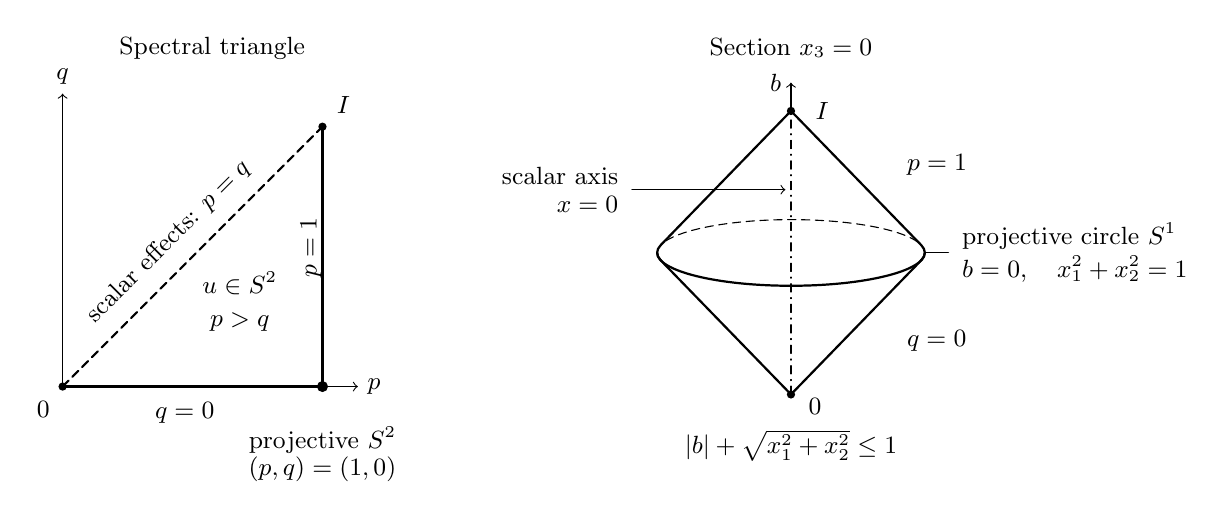
\begin{tikzpicture}[x=1cm,y=1cm,line cap=round,line join=round,
                    font=\small]
  % Left panel: exact ordered spectral triangle.
  \node at (1.9,4.30) {Spectral triangle};
  \draw[->,thin] (0,0) -- (3.75,0) node[right] {$p$};
  \draw[->,thin] (0,0) -- (0,3.72) node[above] {$q$};
  \draw[thick] (0,0) -- (3.3,0) -- (3.3,3.3);
  \draw[thick,densely dashed] (0,0) -- (3.3,3.3);
  \node[rotate=45,anchor=south] at (1.53,1.65)
    {scalar effects: $p=q$};
  \node[anchor=north] at (1.55,-0.08) {$q=0$};
  \node[rotate=90,anchor=south] at (3.41,1.77) {$p=1$};
  \node[align=center] at (2.25,1.08) {$u\in S^2$\\[1pt]$p>q$};
  \fill (0,0) circle (1.5pt);
  \fill (3.3,3.3) circle (1.5pt);
  \fill (3.3,0) circle (2pt);
  \node[anchor=north east] at (-0.04,-0.06) {$0$};
  \node[anchor=south west] at (3.36,3.34) {$I$};
  \node[anchor=north,align=center] at (3.30,-0.39)
    {projective $S^2$\\[-1pt]$(p,q)=(1,0)$};

  % Right panel: a three-dimensional section, shown in linear projection.
  % In local coordinates the map is
  % (x_1,x_2,b) -> (1.70*x_1,0.42*x_2+1.80*b).
  % The cone silhouette meets the projected unit circle at its exact
  % tangency points: sin(alpha)=0.42/1.80=7/30.
  \begin{scope}[shift={(9.25,1.70)}]
    \node at (0,2.60) {Section $x_3=0$};
    \pgfmathsetmacro{\tangentangle}{asin(7/30)}
    \pgfmathsetmacro{\tangentx}{1.70*cos(\tangentangle)}
    \pgfmathsetmacro{\tangenty}{0.42*sin(\tangentangle)}

    \draw[thin,densely dashed] (1.70,0)
      arc[start angle=0,end angle=180,x radius=1.70,y radius=0.42];
    \draw[thick] (-1.70,0)
      arc[start angle=180,end angle=360,x radius=1.70,y radius=0.42];
    \draw[thick] (-\tangentx,\tangenty) -- (0,1.80)
      -- (\tangentx,\tangenty);
    \draw[thick] (-\tangentx,-\tangenty) -- (0,-1.80)
      -- (\tangentx,-\tangenty);
    \draw[thick] (\tangentx,-\tangenty)
      arc[start angle=-\tangentangle,end angle=\tangentangle,
          x radius=1.70,y radius=0.42];
    \draw[thick] (-\tangentx,\tangenty)
      arc[start angle=180-\tangentangle,end angle=180+\tangentangle,
          x radius=1.70,y radius=0.42];

    \draw[thin,dash dot] (0,-1.80) -- (0,1.80);
    \draw[->,thin] (0,1.80) -- (0,2.16) node[left] {$b$};
    \fill (0,1.80) circle (1.5pt);
    \fill (0,-1.80) circle (1.5pt);
    \node[anchor=west] at (0.19,1.80) {$I$};
    \node[anchor=north west] at (0.10,-1.73) {$0$};
    \node[anchor=east,align=right] at (-2.07,0.80)
      {scalar axis\\[-1pt]$x=0$};
    \draw[->,thin] (-2.02,0.80) -- (-0.07,0.80);
    \node[anchor=west] at (1.35,1.12) {$p=1$};
    \node[anchor=west] at (1.35,-1.12) {$q=0$};
    \draw[thin] (1.71,0) -- (2.00,0);
    \node[anchor=west,align=left] at (2.05,0)
      {projective circle $S^1$\\[1pt]$b=0,\quad x_1^2+x_2^2=1$};
    \node[anchor=north] at (0,-2.13)
      {$|b|+\sqrt{x_1^2+x_2^2}\le1$};
  \end{scope}
\end{tikzpicture}
\caption{The four-dimensional effect body $|b|+|x|\le1$.
Each point of the spectral triangle with $p>q$ carries a direction
$u\in S^2$; on the scalar diagonal all directions represent the same
effect. The boundary pieces $q=0$ and $p=1$ meet at the projective stratum
$(p,q)=(1,0)$, which carries the full sphere $S^2$.
The right panel is a projection of the three-dimensional section
$x_3=0$; its equatorial circle is the intersection of that sphere
with the section.}
\label{fig:effectbody76}
\end{figure}

\section{The description entropy of all binary qubit effects}\label{sec:biasedentropy75}
Let
\[
 \mathfrak E=\{E=E^*\in\C^{2\times2}:0\le E\le I\}.
\]
An effect $E$ specifies the ordered measurement with effects $E,I-E$.
Write $\mathcal C_N(\mathfrak E,\delta)$ for its covering number under
$d_N$, allowing arbitrary legal memoryless centres of this interface,
and write $\mathcal C_N^{\mathrm{rat}}(\mathfrak E,\delta)$ when the
centres have rational Cartesian coordinates. Both eigenvalues and the
eigenspaces are charged. The spectral representation
$E=pP_u+q(I-P_u)$, $p\ge q$, represents a scalar effect only once,
independently of $u$.

\begin{theorem}[The full effect body]\label{thm:biasedcover75}
There are absolute constants $c,C,\delta_0>0$ such that, for every integer
$N\ge1$ and $0<\delta\le\delta_0$,
\begin{equation}\label{eq:biasedcover75}
 cN^2\log(N+2)\,\delta^{-4}
 \le \mathcal C_N(\mathfrak E,\delta)
 \le \mathcal C_N^{\mathrm{rat}}(\mathfrak E,\delta)
 \le CN^2\log(N+2)\,\delta^{-4}.
\end{equation}
Consequently the optimum fixed-length reusable payload is
\begin{equation}\label{eq:biasedbits75}
 2\log_2N+\log_2\log(N+2)+4\log_2(1/\delta)+O(1).
\end{equation}
The constants are uniform over the whole closed effect body, including
scalar, deterministic and projective effects. For rational accuracy
input, rational target data admit an exact rational encoder attaining
this order.
\end{theorem}
The logarithm records accumulation near the projective stratum, where
both outcome probabilities can approach their support endpoints.
We prove the upper bound by a finite rational construction and the
lower bound by separated families of projective-corner boxes.

\subsection{A rational spectral and angular code}
For $N\ge1$ and rational $0<\delta\le1/4$, put
\begin{equation}\label{eq:biasedspectralgrid75}
 B=\left\lceil\sqrt{64N/\delta^2}\right\rceil,\qquad
 s_i=\begin{cases}
 \displaystyle\frac{i^2}{B^2+i^2},&0\le i\le B,\\[2mm]
 \displaystyle1-\frac{(2B-i)^2}{B^2+(2B-i)^2},&B<i\le2B.
 \end{cases}
\end{equation}
Thus $0=s_0<s_1<\cdots<s_{2B}=1$. For $0\le j<i\le2B$ define
\begin{equation}\label{eq:biasedangulargrid75}
 K_{ij}^2=
 \frac{N(s_i-s_j)^2}
 {s_i(1-s_i)+s_j(1-s_j)+N^{-1}},\qquad
 A_{ij}=\max\left\{1,
      \left\lceil\sqrt{256K_{ij}^2/\delta^2}\right\rceil\right\}.
\end{equation}
Use the six signed stereographic charts
\begin{equation}\label{eq:biasedsphere75}
 u_a=\epsilon\frac{1-|z|^2}{1+|z|^2},\qquad
 u_b=\frac{2z_b}{1+|z|^2}\quad(b\ne a),\qquad
 a\in\{1,2,3\},\quad \epsilon\in\{-1,1\},
\end{equation}
with $z\in\{-A_{ij},\ldots,A_{ij}\}^2/A_{ij}$ for the spectral
pair $(s_i,s_j)$. Every chart word decodes to
$s_iP_u+s_j(I-P_u)$. A diagonal pair $i=j$ has the single word
$s_iI$. The exact number of words, including redundant chart words,
is
\begin{equation}\label{eq:biasedcapacity75}
 L_{N,\delta}=(2B+1)+
       \sum_{0\le j<i\le2B}6(2A_{ij}+1)^2.
\end{equation}

\begin{theorem}[Exact rational realization]\label{thm:biasedcodec75}
The words in \eqref{eq:biasedcapacity75} form a radius-$\delta/2$
cover of $\mathfrak E$ by legal rational effects, and
\begin{equation}\label{eq:biasedcapacitybound75}
 L_{N,\delta}\le C N^2\log(N+2)\,\delta^{-4}
\end{equation}
for an absolute $C$. If
\[
 E=\tfrac12\bigl((1+b)I+x\cdot\sigma\bigr),\qquad
 b\in\Q,\quad x\in\Q^3,\quad |b|+|x|\le1,
\]
then a covering word is computable by rational arithmetic and integer
comparisons. Its payload is one fixed-length index in the set of
\eqref{eq:biasedcapacity75}.
\end{theorem}
\begin{proof}
Write $f(t)=t^2/(1+t^2)$, $0\le t\le1$. For a probability in
$[0,1/2]$, round its inverse coordinate $t$ to the nearest multiple
of $1/B$; for a probability in $[1/2,1]$, use the reflected chart
$1-f(t)$. Choose the multiple of smaller magnitude at ties. This
defines a nondecreasing quantizer on $[0,1]$, so separately quantizing
$p\ge q$ preserves their order.

The square-root vector associated with $f(t)$ is
$(t,1)/\sqrt{1+t^2}$; its derivative has norm $1/(1+t^2)\le1$.
The reflected chart has the same bound. Hence the Euclidean
square-root distance between each probability and its quantization
is at most $1/(2B)$. If $H$ is this distance, the product-fidelity
inequality gives unhalved distance at most $2\sqrt N H$ between the
corresponding $N$-fold Bernoulli laws. The common two-coin programme
in Lemma~\ref{lem:spectralprojection75} therefore gives a spectral error
at most
\[
                         2\sqrt N/B\le\delta/4.
\]
This argument includes adaptive testers and entangled references.

If the quantized eigenvalues coincide, this completes the encoding.
Otherwise choose a signed chart whose distinguished coordinate has
maximal absolute value in the target direction. Its inverse coordinate
belongs to $[-1,1]^2$. Rounding its two coordinates to the grid of
denominator $A_{ij}$ gives angular error at most $2\sqrt2/A_{ij}$,
since geodesic distance is bounded by the length of the mapped
straight segment and the differential of stereographic projection has
norm at most two. The angular upper bound in Theorem~\ref{thm:biasedangular75}
gives error at most
\[
 \sqrt2 K_{ij}\frac{2\sqrt2}{A_{ij}}
                   \le\delta/4.
\]
The triangle inequality proves the covering assertion. Formula
\eqref{eq:biasedsphere75} preserves the unit sphere exactly, so every
decoded effect is legal and rational.

We verify exact computability even when the input eigenvalues are
irrational. Put $Q=|x|^2\in\Q$. The eigenvalues are
$(1+b\pm\sqrt Q)/2$. Each decision in the spectral rounding compares
one of these numbers with a rational threshold $f((k+1/2)/B)$ or its
reflection. Such a comparison is the sign of a rational number plus
or minus $\sqrt Q$; checking signs before squaring makes it an exact
rational comparison. If $Q=0$, the two quantized eigenvalues coincide.
Otherwise choose the smallest index $a$ maximizing $|x_a|$ and put
$\epsilon=\operatorname{sgn}(x_a)$. The inverse chart is
\[
                    z_b=\frac{x_b}{\sqrt Q+|x_a|}\quad(b\ne a).
\]
Its comparison with any rational rounding threshold again reduces
to the sign of a rational number plus a rational multiple of
$\sqrt Q$. The integers $B,A_{ij}$ are computed by integer squaring
and rational comparison. Thus no irrational normalization is required.
The decoder uses only the displayed rational formulae.

It remains to count the words. Set $m_i=\min(i,2B-i)$ and
$U=B^2/N$. Directly from \eqref{eq:biasedspectralgrid75},
\[
 \frac{m_i^2}{4B^2}\le s_i(1-s_i)\le\frac{m_i^2}{B^2},\qquad
 K_{ij}^2\le
          \frac{4NB^2}{m_i^2+m_j^2+U}.
\]
Each value of $m_i$ occurs at most twice. Since
$(2A_{ij}+1)^2\le C(1+K_{ij}^2/\delta^2)$, we obtain
\begin{equation}\label{eq:biasedlattice75}
 L_{N,\delta}\le CB^2+
 \frac{CNB^2}{\delta^2}
       \sum_{a,b=0}^{B}\frac1{a^2+b^2+U}.
\end{equation}
Here $U\ge1$. The part with $\max(a,b)\le\sqrt U$ is bounded by an
absolute constant. Each successive dyadic square ring contributes
at most another absolute constant. There are at most
$C\log(N+2)$ such rings, because $B/\sqrt U=\sqrt N$. Consequently
\[
              \sum_{a,b=0}^{B}\frac1{a^2+b^2+U}
                       \le C\log(N+2).
\]
Finally $B^2\le CN/\delta^2$, so \eqref{eq:biasedlattice75} proves
\eqref{eq:biasedcapacitybound75}. The support cutoff in the denominator
is retained throughout the count, including the endpoint grid words.
\end{proof}

\subsection{Packing the projective corner}
\begin{proof}[Proof of Theorem~\ref{thm:biasedcover75}]
The upper bound follows from Theorem~\ref{thm:biasedcodec75}. For a
real $\delta$, choose a rational $\delta'$ with
$\delta\le\delta'\le2\delta$ and use its radius-$\delta'/2$ code;
decrease $\delta_0$ to at most $1/8$. For the lower bound first let
$N\ge16$. For every
\[
                     t=8^j/N\le1/16,\qquad j\ge0,
\]
consider the effects with
\begin{equation}\label{eq:biasedcorner75}
 p=1-\alpha,\quad q=\beta,\quad
 t\le\alpha,\beta\le2t,\qquad
 u=u(z),\quad z\in[-1/4,1/4]^2,
\end{equation}
where $u(z)$ is the chart in \eqref{eq:biasedsphere75} with
$a=3,\epsilon=1$. On this square, spherical distance is bounded
above and below by absolute positive multiples of Euclidean distance
in $z$. Throughout \eqref{eq:biasedcorner75}, the eigenvalue gap is
at least $3/4$ and
\[
 p(1-p)\asymp q(1-q)\asymp t,\qquad
 p(1-p)+q(1-q)+N^{-1}\asymp t.
\]
The finite-distance comparison of Theorem~\ref{thm:biasedmetric75}
therefore supplies an absolute $c_1>0$ such that any two points in
this box satisfy
\begin{equation}\label{eq:biasedboxmetric75}
 d_N\ge c_1\min\left\{1,
       \sqrt{N/t}\,
       \bigl| (\alpha,\beta,z)-
              (\alpha',\beta',z')\bigr|_\infty\right\}.
\end{equation}
Choose an absolute sufficiently large $A$ and then an absolute
sufficiently small $\delta_0$. In each of the four coordinates take
a grid of spacing $A\delta\sqrt{t/N}$. Since $Nt\ge1$, this spacing
is at most half the width of either spectral interval when
$\delta\le\delta_0$. The resulting points have pairwise distance
at least $4\delta$ by \eqref{eq:biasedboxmetric75}, and their number
is at least
\[
 c\left(\frac{t}{\delta\sqrt{t/N}}\right)^2
   \left(\frac1{\delta\sqrt{t/N}}\right)^2
                         =cN^2\delta^{-4}.
\]

Points from different boxes are also uniformly separated. Indeed,
if $t'\ge8t$, then $\alpha'\ge t'$ and $\alpha\le2t\le t'/4$.
The spectral modulus of the corresponding upper eigenvalues is
bounded below by an absolute positive multiple of
$\sqrt{Nt'}\ge1$. The spectral noncancellation bound in
Theorem~\ref{thm:biasedmetric75} gives $d_N\ge c_2>0$.
Shrinking $\delta_0$ ensures that this is at least $4\delta$.
There are at least $c\log(N+2)$ permitted boxes. Their union is
therefore a $4\delta$-packing of cardinality
$cN^2\log(N+2)\delta^{-4}$.

For $1\le N<16$, use instead a fixed spectral rectangle
$5/8\le p\le3/4$, $1/4\le q\le3/8$ and the same angular chart.
Theorem~\ref{thm:biasedmetric75} gives a uniform local Euclidean lower
bound, and a grid of spacing $C\delta$ has at least $c\delta^{-4}$
points. The factor $N^2\log(N+2)$ is bounded on this finite range.
This proves the same lower estimate for all $N\ge1$.

A radius-$\delta$ ball about any legal centre contains at most one
point of a $4\delta$-packing, by the triangle inequality. Hence the
packing proves the lower bound with the stated centre convention.
Taking binary logarithms and rounding the index length proves
\eqref{eq:biasedbits75}.
\end{proof}

\subsection{The source of the logarithm}
The spectral and angular weights also give the following integral
form of the same accumulation. Put $v_p=p(1-p)$, $v_q=q(1-q)$ and
$\tau=N^{-1}$. Then
\begin{equation}\label{eq:biasedvolume75}
 \int_{0\le q\le p\le1}
 \frac{N^2(p-q)^2\,dp\,dq}
 {(v_p+v_q+\tau)\sqrt{(v_p+\tau)(v_q+\tau)}}
                         \asymp N^2\log(N+2).
\end{equation}
To verify this, near $p=1,q=0$ put $\alpha=1-p$, $\beta=q$.
After removing the factor $N^2$, the integrand is comparable to
\[
 \frac1{(\alpha+\beta+\tau)
             \sqrt{(\alpha+\tau)(\beta+\tau)}}.
\]
For $s=\alpha+\beta$, integration over $0\le\alpha\le s$ is
bounded above by an absolute constant times $1/(s+\tau)$.
For $s\ge2\tau$, restriction to $s/4\le\alpha\le3s/4$ gives the
matching lower bound. Integration in $s$ proves logarithmic growth.
Near the scalar endpoint $p=q=0$, the factor $(p-q)^2$ is at most
$(p+q)^2$, while $v_p+v_q\asymp p+q$; the remaining integral is
uniformly bounded. Complementation gives the same conclusion near
$p=q=1$. Away from these endpoint neighbourhoods,
$v_p+v_q$ is bounded below and the factors $v_p^{-1/2},v_q^{-1/2}$
are integrable. Bounded $N$ is absorbed into the constants.
Thus the extra logarithm is contributed by the projective corner.
The finite covering construction and packing above also include the
collapsed scalar coordinates, where the spectral representation
ceases to be a chart.

\section{Matrix geometry in arbitrary input dimension}
\label{sec:matrixmetric76}

The binary effect body has a finite-use description that does not
require eigenvector coordinates.  Its regularization is the same at
every spectral rank, and two-dimensional compressions supply lower
witnesses for the full matrix problem.  Throughout this section
$d,N\ge1$ are integers and
\begin{equation}\label{eq:matrixbody76}
 \mathfrak E_d=\{E\in\End(\C^d):E=E^*,\ 0\preceq E\preceq I_d\}.
\end{equation}
The measurement $\mathcal M_E$ has the ordered effects $E,I_d-E$
and no residual quantum output.  The distance $d_N$ has the same
reference-assisted adaptive meaning as in
Theorem~\ref{thm:biasedmetric75}.  Write $d_N^{\rm na}$ for its
restriction to nonadaptive experiments, allowing entanglement across
the calls and a retained reference.  These experiments may depend on
the known pair of hypotheses.

Put $\tau=N^{-1}$ and $V_E=E(I_d-E)$.  On the real Hilbert space
of Hermitian matrices with Hilbert--Schmidt inner product, define
\begin{align}
 \mathcal A_E(H)&=V_EH+HV_E+\tau H,
                                      \label{eq:matrixoperator76}\\
 g_{N,E}(H)^2&=N\ip{H}{\mathcal A_E^{-1}(H)}_{\rm HS}.
                                      \label{eq:matrixform76}
\end{align}
The operator $\mathcal A_E$ is strictly positive, including at a
singular effect.  For a pair $E,F$ set
\begin{equation}\label{eq:matrixmodulus76}
 M=\tfrac12(E+F),\qquad H=F-E,\qquad
 Q_N(E,F)=g_{N,M}(H).
\end{equation}
In any orthonormal eigenbasis of $M$, with eigenvalues $m_i$ and
$v_i=m_i(1-m_i)$, this is
\begin{equation}\label{eq:matrixcoordinates76}
 Q_N(E,F)^2=N\sum_{i,j=1}^d
                \frac{|H_{ij}|^2}{v_i+v_j+N^{-1}}.
\end{equation}
Definition~\eqref{eq:matrixmodulus76} makes the expression independent
of all choices at repeated eigenvalues.  We use it as a comparison
modulus; a triangle inequality for $Q_N$ is not required.

The inverse Sylvester operator is familiar from the Bures metric
$g^{\rm B}$ on the positive definite cone \cite{Dittmann76}.
Its normalization gives the algebraic identity
\[
 g_{N,E}(H)^2=2N\,g^{\rm B}_{V_E+\tau I_d/2}(H,H).
\]
Here $H$ remains the effect tangent; the differential of the
variance map $E\mapsto V_E$ is $H-EH-HE$.

\begin{theorem}[Finite-use geometry of the matrix effect body]
\label{thm:matrixmetric76}
For every $E,F\in\mathfrak E_d$,
\begin{equation}\label{eq:matrixmetric76}
 \frac1{8192d}\min\{1,Q_N(E,F)\}
 \le d_N^{\rm na}(\mathcal M_E,\mathcal M_F)
 \le d_N(\mathcal M_E,\mathcal M_F)
 \le\min\{2,8Q_N(E,F)\}.
\end{equation}
The constants are uniform in the horizon and in both effects,
without a spectral margin or a condition on eigenvalue multiplicities.
The adaptive upper bound permits arbitrary retained references,
common feedback, and bounded public stopping.  Each lower witness
uses inputs in one fixed subspace of dimension at most two.  Moreover,
\begin{equation}\label{eq:matrixoneuse76}
 d_1(\mathcal M_E,\mathcal M_F)=2\|E-F\|_{\rm op}.
\end{equation}
\end{theorem}

The theorem includes every rank of projection and all of the
intermediate singular strata.  The variance $E(I_d-E)$, rather than
the smallest eigenvalue of either outcome, determines the matrix
weights.  The factor $N^{-1}$ makes the formula finite on the entire
closed body.  The proof first establishes a path inequality valid for
every common adaptive tester, and then obtains the converse from
one- and two-dimensional experiments.

\subsection{A horizontal measurement dilation}

Kraus-gauge bounds for channel estimation were developed in
\cite{FI76,DKG67,DM76}.  Their integration along channel paths
appears in \cite[Section~III, equation~(26)]{YF76} and, with
general adaptive bounds, in \cite[Section~IV.A]{SD76}.  We use an
explicit horizontal lift for binary effects and control the
finite-horizon regularization by a trace-norm remainder.

\begin{lemma}[Horizontal derivative and regularized path bound]
\label{lem:matrixpath76}
Every continuously differentiable path $G:[0,1]\to\mathfrak E_d$
satisfies
\begin{equation}\label{eq:matrixpath76}
 d_N(\mathcal M_{G(0)},\mathcal M_{G(1)})
       \le4\int_0^1 g_{N,G(t)}(G'(t))\,dt.
\end{equation}
\end{lemma}
\begin{proof}
We begin with an interior effect $G$, so that $G$ and $I_d-G$
are invertible.  Set $S=\sqrt{G(I_d-G)}$.  For a Hermitian matrix
$K$ put $H_0=SK+KS$.  At the two factors
$A_1=\sqrt G$, $A_0=\sqrt{I_d-G}$ prescribe derivatives
\begin{equation}\label{eq:horizontalderivatives76}
 B_1=\sqrt{I_d-G}\,K,\qquad B_0=-\sqrt G\,K.
\end{equation}
They obey
\begin{align}
 A_1^*B_1+B_1^*A_1&=H_0,&
 A_0^*B_0+B_0^*A_0&=-H_0,\notag\\
 \sum_{y=0}^1 A_y^*B_y&=0,&
 \sum_{y=0}^1 B_y^*B_y&=K^2.
                                      \label{eq:horizontalidentities76}
\end{align}

These tangent equations can be realized by genuine dilations.
Let $G_1(s)=G+sH_0$, $G_0(s)=I_d-G-sH_0$ for $s$ in a
sufficiently small open interval, and put $R_y(s)=\sqrt{G_y(s)}$.
The first line of \eqref{eq:horizontalidentities76} implies that
\[
 T_y=(B_y-R_y'(0))R_y(0)^{-1}
\]
is anti-Hermitian.  Indeed, multiplying $T_y+T_y^*$ on the left
and right by $R_y(0)$ gives, with $R=R_y(0)$,
\[
 R(T_y+T_y^*)R=RB_y+B_y^*R-(RR_y'(0)+R_y'(0)R)=0,
\]
by differentiating $R_y(s)^2=G_y(s)$.  Thus
$\widetilde A_y(s)=\exp(sT_y)R_y(s)$ has derivative $B_y$ at
zero and satisfies
$\widetilde A_y(s)^*\widetilde A_y(s)=G_y(s)$ exactly.  A measurement
isometry is
\[
 W(s)\psi=\sum_{y=0}^1
              |y\rangle_C|y\rangle_L\widetilde A_y(s)\psi.
\]
Here $C$ is the observed outcome, and $L$ and the factor space of
$\widetilde A_y$ are environments.  Tracing the environments
implements $\mathcal M_{G(s)}$, also on inputs entangled with a
reference.  At zero, \eqref{eq:horizontalidentities76} gives
\begin{equation}\label{eq:horizontaloverlap76}
 W^*\dot W=0,\qquad \dot W^*\dot W=K^2.
\end{equation}

The horizontal Kraus condition has the antecedents
\cite[Theorems~4--5]{FI76}. Its adaptive channel-extension form is
$F_N\le4N\|\alpha\|$ when $\beta=0$; see
\cite[equation~(9)]{DM76} and \cite[equations~(5)--(10)]{KGAD76}.
In the present lift $\alpha=K^2$ and $\beta=0$. We give the cancellation
explicitly for this binary measurement.

Fix a common tester with $N$ slots.  Purify its initial state and
all intervening operations, and retain the measurement environments
only for this comparison; neither the outcome copy nor the factor
environment is accessible to the tester.  The derivative of its final purification
in the direction $H_0$ is the sum of $N$ terms, each having one
differentiated occurrence of $W$.  The terms are mutually orthogonal.
For two different differentiated slots, cancel the common isometries
after the later slot; the remaining overlap contains
$W^*\dot W\otimes I=0$.  Each term has norm at most
$\|\dot W\|_{\rm op}=\|K\|_{\rm op}$, independently of the
reference and memory dimensions.  Hence the derivative of the
purification has norm at most $\sqrt N\|K\|_{\rm op}$.
The pure-state trace-norm derivative bound, followed by contraction
under the partial trace, bounds the observed output derivative by
\begin{equation}\label{eq:horizontaltangent76}
 2\sqrt N\|K\|_{\rm op}.
\end{equation}
A publicly stopped tester is padded to $N$ slots by calls on fixed
dummy inputs, whose outcomes and environments are both discarded.  The same purification
argument then applies to its original output.  Classical feedback is
included by purifying the common controlled operations.

Now let $H$ be an arbitrary Hermitian tangent at $G$, and set
$\kappa=N^{-1/2}$.  There is a unique Hermitian solution of
\begin{equation}\label{eq:regularizedsylvester76}
 SK+KS+\kappa K=H.
\end{equation}
Write $H=H_0+R$, with $H_0=SK+KS$ and $R=\kappa K$.
Both are legitimate tangents at the interior effect $G$.  The
derivative of a fixed tester's output is linear in the inserted
channel tangent.  The part arising from $H_0$ is bounded by
\eqref{eq:horizontaltangent76}.  The part arising from $R$ is
bounded by $2N\|R\|_{\rm op}$.  To verify the latter bound,
the one-call tangent has two opposite reference blocks
\[
 B_\rho=\tr_A[(R\otimes I)\rho],\qquad -B_\rho.
\]
Duality against Hermitian contractions gives
$\|B_\rho\|_1\le\|R\|_{\rm op}$ for every input state.
Insert this tangent into each of the $N$ slots in turn; all
subsequent common channels contract the Hermitian trace norm.
This proves the bound for its sum.  Thus the actual tangent $H$
has output derivative bounded by
\begin{equation}\label{eq:regularizedtangent76}
 2\sqrt N\|K\|_{\rm op}+2N\|R\|_{\rm op}
                         =4\sqrt N\|K\|_{\rm op}.
\end{equation}
The splitting is used only for the differential at an interior
effect; it does not postulate a physical mixture realizing the
entire path.

In an eigenbasis of $G$, with $v_i=g_i(1-g_i)$, equation
\eqref{eq:regularizedsylvester76} reads
\[
 K_{ij}=\frac{H_{ij}}{\sqrt{v_i}+\sqrt{v_j}+\kappa}.
\]
Since $(\sqrt{v_i}+\sqrt{v_j}+\kappa)^2\ge v_i+v_j+\tau$,
\begin{equation}\label{eq:regularizedformbound76}
 \sqrt N\|K\|_{\rm op}
 \le\sqrt N\|K\|_{\rm HS}
 \le g_{N,G}(H).
\end{equation}
The integration of local distinguishability has direct antecedents:
\cite[Section~III, equation~(26), PDF version~3]{YF76} treats the
parallel path bound, and
\cite[Section~IV.A, equations~(14)--(22)]{SD76} applies adaptive
metrological estimates. Here the regularized binary Sylvester split
and its residual produce the explicit integrand.
For an interior path, integrate the resulting output derivative
bound for each fixed tester, and then take the supremum.  This
proves \eqref{eq:matrixpath76} without exchanging a supremum
with a derivative.

For a path in the closed body, apply the result to
$G_\epsilon(t)=(1-2\epsilon)G(t)+\epsilon I_d$, where
$0<\epsilon<1/2$.  At fixed $N$, the form
$g_{N,G}(H)$ is continuous on the whole body and bounded above
by $N\|H\|_{\rm HS}$.  The integrals therefore converge as
$\epsilon\downarrow0$.  The hybrid inequality
$d_N(\mathcal M_E,\mathcal M_F)\le2N\|E-F\|_{\rm op}$
gives continuity of the distances at both endpoints.  Passing to
the limit proves the asserted closed-body statement.
\end{proof}

\subsection{The midpoint comparison}

\begin{proof}[Proof of Theorem~\ref{thm:matrixmetric76}]
For the upper bound use $G(t)=(1-t)E+tF$.  The map
$G\mapsto V_G=G-G^2$ is operator concave.  For $0<t\le1/2$,
write $G(t)=(1-2t)E+2tM$ and discard the positive multiple of
$V_E$ in the concavity inequality.  Applying the same argument
from the other endpoint gives
\begin{equation}\label{eq:midpointvariance76}
 V_{G(t)}\succeq a(t)V_M,\qquad
             a(t)=2\min\{t,1-t\}.
\end{equation}
For a positive matrix $D$ and a Hermitian matrix $X$,
\[
 \langle X,(L_D+R_D)X\rangle_{\rm HS}
       =2\operatorname{tr}(DX^2)\ge0.
\]
Thus left-plus-right multiplication preserves the stated order on the
real Hilbert space of Hermitian matrices.  Since $a(t)\le1$,
$\mathcal A_{G(t)}\succeq a(t)\mathcal A_M$.
Inverting positive operators reverses their order, whence
\[
 g_{N,G(t)}(H)\le a(t)^{-1/2}Q_N(E,F).
\]
The scalar factor has integral $2$ on $[0,1]$.
Lemma~\ref{lem:matrixpath76} yields $d_N\le8Q_N$;
the trace-norm bound $d_N\le2$ gives the stated upper estimate.

For the lower bound choose any orthonormal eigenbasis $e_i$ of
$M$ and put
\begin{equation}\label{eq:matrixentries76}
 q_{ij}=|H_{ij}|\sqrt{\frac N{v_i+v_j+\tau}},
                 \qquad Q_N^2=\sum_{i,j}q_{ij}^2.
\end{equation}
Repeated input $e_i$ gives Bernoulli probabilities
$s=m_i-H_{ii}/2$, $t=m_i+H_{ii}/2$.  Their variances satisfy
\[
 \max\{s(1-s),t(1-t)\}
 \le s(1-s)+t(1-t)\le2m_i(1-m_i).
\]
Lemma~\ref{lem:bernoulliproduct75} therefore gives
\begin{equation}\label{eq:matrixdiagonallower76}
 d_N^{\rm na}(\mathcal M_E,\mathcal M_F)
                            \ge\tfrac1{64}\min\{1,q_{ii}\}.
\end{equation}

For $i\ne j$, restrict each input to
$\mathcal S=\spanop\{e_i,e_j\}$.  The resulting channels have
the compressed effects $E_{\mathcal S},F_{\mathcal S}$, including
on inputs entangled with a retained reference.  Their midpoint is
$M_{\mathcal S}=\diag(m_i,m_j)$.  Write their spectral data as
$(p,q,u)$ and $(p',q',v)$ in the notation of
Section~\ref{sec:biasedmetric75}, with gaps $r,r'$ and angle $h$
when both gaps are positive.  Put
\[
 V_E^{\mathcal S}=p(1-p)+q(1-q),\qquad
 V_F^{\mathcal S}=p'(1-p')+q'(1-q').
\]
For the compressed matrices the exact identity
\[
 V_{M_{\mathcal S}}=\tfrac12V_{E_{\mathcal S}}
              +\tfrac12V_{F_{\mathcal S}}
              +\tfrac14(F_{\mathcal S}-E_{\mathcal S})^2
\]
shows, on taking traces, that
\begin{equation}\label{eq:compressionvariance76}
 v_i+v_j+\tau\ge\tfrac12(V_E^{\mathcal S}+\tau),
 \qquad
 v_i+v_j+\tau\ge\tfrac12(V_F^{\mathcal S}+\tau).
\end{equation}
The scalar part of $F_{\mathcal S}-E_{\mathcal S}$ has zero
off-diagonal entry.  Its traceless part has operator norm
$|ru-r'v|/2$.  Decomposing this vector along the smaller radius
gives
\begin{align}
 |H_{ij}|&\le\tfrac12|r-r'|+\min\{r,r'\}\sin(h/2)\notag\\
 &\le\tfrac12\bigl(|p-p'|+|q-q'|+\min\{r,r'\}h\bigr).
                                      \label{eq:compressionoffdiagonal76}
\end{align}
When one radius is zero, the angular term is zero and the same
inequality holds without choosing its direction.  Each endpoint
variance is bounded by the appropriate $V_E^{\mathcal S}$ or
$V_F^{\mathcal S}$.  Equations
\eqref{eq:compressionvariance76}--\eqref{eq:compressionoffdiagonal76}
therefore imply
\begin{equation}\label{eq:compressionmodulus76}
 q_{ij}\le\frac1{\sqrt2}
 \left(T_N(p,p')+T_N(q,q')
       +\min\{K_N(p,q),K_N(p',q')\}h\right).
\end{equation}
The nonadaptive assertion of Theorem~\ref{thm:biasedmetric75}
applied to this compressed pair yields
\begin{equation}\label{eq:matrixoffdiagonallower76}
 d_N^{\rm na}(\mathcal M_E,\mathcal M_F)
                         \ge\tfrac1{8192}\min\{1,q_{ij}\}.
\end{equation}
Every such witness is a legitimate experiment for the original
effects by a fixed isometric embedding of $\mathcal S$.
Since $\max_{i,j}q_{ij}\ge Q_N/d$, taking the strongest of
\eqref{eq:matrixdiagonallower76} and
\eqref{eq:matrixoffdiagonallower76} proves the lower bound.
For $d=1$ only the diagonal argument is needed.

Finally, a one-use reference-assisted difference has output blocks
$B_\rho$ and $-B_\rho$, with
$B_\rho=\tr_A[((E-F)\otimes I)\rho]$.  Trace-norm duality
against Hermitian contractions gives
$\|B_\rho\|_1\le\|E-F\|_{\rm op}$.  An eigenstate of
$E-F$ at an extremal eigenvalue attains equality.  This proves
\eqref{eq:matrixoneuse76}.
\end{proof}

\begin{corollary}[Uniform comparison with nonadaptive experiments]
\label{cor:matrixadaptivity76}
For all $E,F\in\mathfrak E_d$ and all $N\ge1$,
\begin{equation}\label{eq:matrixadaptivity76}
 d_N(\mathcal M_E,\mathcal M_F)
           \le65536d\,d_N^{\rm na}(\mathcal M_E,\mathcal M_F).
\end{equation}
Here nonadaptive experiments may entangle all inputs and retain a
reference; they use no feedback between calls. The dimensional constant
comes from the maximum of $d^2$ weighted entries and is not optimized.
\end{corollary}
\begin{proof}
If $Q_N\le1$, divide the upper estimate $8Q_N$ by the lower
estimate $Q_N/(8192d)$.  If $Q_N\ge1$, the upper estimate is
$2$ and the lower estimate is $1/(8192d)$, which gives a smaller
constant.  The identical pair needs no division.
\end{proof}

\subsection{All spectral ranks and local forms}

\begin{lemma}[Spectral noncancellation in every rank]
\label{lem:matrixspectral76}
Let $\lambda_1(E)\ge\cdots\ge\lambda_d(E)$ and
$\lambda_1(F)\ge\cdots\ge\lambda_d(F)$ be the ordered spectra.
For every $1\le k\le d$,
\begin{equation}\label{eq:matrixspectrallower76}
 B_N(\lambda_k(E),\lambda_k(F))
                   \le d_N^{\rm na}(\mathcal M_E,\mathcal M_F).
\end{equation}
For effects diagonal in the same ordered orthonormal basis,
\begin{equation}\label{eq:matrixspectralupper76}
 d_N(\mathcal M_E,\mathcal M_F)
       \le\sum_{k=1}^d B_N(\lambda_k(E),\lambda_k(F)).
\end{equation}
\end{lemma}
\begin{proof}
Suppose $\lambda_k(E)\ge\lambda_k(F)$.  The span of the first
$k$ eigenvectors of $E$ intersects the orthogonal complement of
the first $k-1$ eigenvectors of $F$ in a nonzero subspace.  A unit
vector in that intersection has success probabilities
$s\ge\lambda_k(E)\ge\lambda_k(F)\ge t$ under the two
hypotheses.  The monotonicity in
Lemma~\ref{lem:bernoulliproduct75} implies
$B_N(s,t)\ge B_N(\lambda_k(E),\lambda_k(F))$.
Repeated use of this vector proves the first assertion; reverse
the hypotheses for the opposite ordering.  Multiplicities cause
no change in the dimension argument.

For the upper bound, first measure the common eigenbasis and then
produce a bit whose success probability is its corresponding
eigenvalue.  Supply $N$ independent bits in each of the $d$ rows
before the experiment.  Every common adaptive tester is a common
channel of these row arrays, including its reference blocks and
all publicly stopped histories.  The tensor-product triangle
inequality gives \eqref{eq:matrixspectralupper76}; unused row
bits are discarded.
\end{proof}

The following local comparison will permit volume estimates at
every boundary stratum.  It concerns matrices themselves and
does not require a coordinate chart for eigenvectors.

\begin{lemma}[Uniform local comparison of the variance forms]
\label{lem:matrixlocal76}
Set $W_G=G(I_d-G)+\tau I_d/2$.  For a Hermitian $H$, put
$q=g_{N,G}(H)$.  Then
\begin{equation}\label{eq:matrixrelative76}
 \|W_G^{-1/2}HW_G^{-1/2}\|_{\rm HS}\le2q.
\end{equation}
For either sign for which $G\pm H/2\in\mathfrak E_d$, one has
\begin{equation}\label{eq:matrixlocalperturbation76}
 \bigl\|W_G^{-1/2}(W_{G\pm H/2}-W_G)W_G^{-1/2}\bigr\|_{\rm op}
                       \le q+\tfrac34q^2.
\end{equation}
In particular, for $q\le1/4$,
\begin{equation}\label{eq:matrixlocalorder76}
 \tfrac12W_G\preceq W_{G\pm H/2}\preceq2W_G.
\end{equation}
Thus, if either $Q_N(E,F)\le1/4$ or
$g_{N,E}(F-E)\le1/4$, the midpoint and the fixed-endpoint
quadratic forms are comparable within factors $2$.
\end{lemma}
\begin{proof}
In an eigenbasis of $W_G$, with eigenvalues $w_i\ge\tau/2$,
\[
 \frac{w_i+w_j}{Nw_iw_j}\le4.
\]
Multiplying this inequality by
$N|H_{ij}|^2/(w_i+w_j)$ and summing proves
\eqref{eq:matrixrelative76}.  Put
$Z=W_G^{-1/2}HW_G^{-1/2}$.  The exact expansion
\[
 W_{G\pm H/2}-W_G
            =\pm\tfrac12(H-GH-HG)-\tfrac14H^2
\]
has normalized linear part
$\pm((I_d-2G)Z+Z(I_d-2G))/4$, since $G$ commutes with
$W_G$.  Its operator norm is at most $\|Z\|_{\rm op}/2\le q$.
The normalized quadratic part is $-ZW_GZ/4$.
Since $\tau\le1$, one has $\|W_G\|_{\rm op}\le3/4$, and
its norm is at most $3q^2/4$.  This proves
\eqref{eq:matrixlocalperturbation76} and hence
\eqref{eq:matrixlocalorder76}.  The same order holds for left
plus right multiplication, and inversion gives the quadratic-form
comparison.  Apply it first at $G=M$ or at $G=E$, respectively,
to obtain the final assertion.
\end{proof}

\section{Description entropy in arbitrary matrix dimension}
\label{sec:matrixentropy76}
The intrinsic comparison of Theorem~\ref{thm:matrixmetric76} permits
the full effect body to be treated without choosing eigenvector
coordinates near repeated spectra. Throughout this section the input
dimension $d\ge1$ is fixed. Constants may depend on $d$, but not on the
integer horizon $N\ge1$ or on the accuracy parameter.

Write $\mathcal C_N(\mathfrak E_d,\delta)$ for the covering number under
$d_N$, with centres in the same legal memoryless ordered binary
interface, and write $\mathcal C_N^{\mathrm{rat}}$ when the real and
imaginary parts of every matrix entry of each centre are rational.

\begin{theorem}[Entropy of the full effect body]\label{thm:matrixcover76}
For every integer $d\ge1$ there are constants $c_d,C_d,\delta_d>0$
such that, for all integers $N\ge1$ and all $0<\delta\le\delta_d$,
\begin{equation}\label{eq:matrixcover76}
\begin{split}
 c_d N^{d^2/2}[\log(N+2)]^{\lfloor d/2\rfloor}\delta^{-d^2}
 &\le \mathcal C_N(\mathfrak E_d,\delta)\\
 &\le \mathcal C_N^{\mathrm{rat}}(\mathfrak E_d,\delta)\\
 &\le C_d N^{d^2/2}[\log(N+2)]^{\lfloor d/2\rfloor}\delta^{-d^2}.
\end{split}
\end{equation}
Consequently the optimum fixed-length reusable description has length
\begin{equation}\label{eq:matrixbits76}
 \frac{d^2}{2}\log_2N
 +\lfloor d/2\rfloor\log_2\log(N+2)
 +d^2\log_2(1/\delta)+O_d(1).
\end{equation}
The estimates include all support and spectral multiplicities. The
rational-centre assertion here follows from a covering argument.
Theorem~\ref{thm:matrixcodec77} gives a deterministic finite exact
encoder and decoder attaining the same order in every dimension.
Theorem~\ref{thm:biasedcodec75} retains its separate direct construction
in dimension two. Computational cost is accounted for separately
from the number of transmitted bits.
\end{theorem}

For $d=1$, the result is the Bernoulli covering law
$N^{1/2}\delta^{-1}$. For $d=2$, it recovers
Theorem~\ref{thm:biasedcover75}. The next two cases have orders
$N^{9/2}\log(N+2)\delta^{-9}$ and
$N^8[\log(N+2)]^2\delta^{-16}$. The logarithmic power counts independent
nested approaches of paired eigenvalues to the two support endpoints.
We first establish a uniform measure estimate for actual operational
balls, and then evaluate the total measure.

\subsection{Operational balls and a regularized volume form}
Set $n=d^2$, $\tau=N^{-1}$ and
\[
 W_E=E(I-E)+\frac\tau2 I.
\]
As in Section~\ref{sec:matrixmetric76}, let
\begin{equation}\label{eq:matrixfixedform76}
 g_{N,E}(H)^2
 =N\langle H,(L_{W_E}+R_{W_E})^{-1}H\rangle_{\mathrm{HS}}
\end{equation}
on the real Hilbert space of Hermitian matrices. Let $G_{N,E}$ denote
this positive quadratic form in Hilbert--Schmidt orthonormal
coordinates, and define
\begin{equation}\label{eq:matrixmeasure76}
 \rho_N(E)=\sqrt{\det G_{N,E}},\qquad
 d\mu_N(E)=\rho_N(E)\,dE,
\end{equation}
The real orthonormal basis consists of $e_{ii}$ and, for $i<j$,
$(e_{ij}+e_{ji})/\sqrt2$ and $\mathrm i(e_{ij}-e_{ji})/\sqrt2$;
$dE$ is Lebesgue measure in these coordinates. The cutoff makes
$\rho_N$ positive and continuous on the whole closed body for each
$N$.

\begin{lemma}[Uniform volume of operational balls]\label{lem:matrixball76}
For fixed $d$ there are $a_d,A_d,r_d>0$ such that
\begin{equation}\label{eq:matrixball76}
 a_dr^{d^2}\le
 \mu_N\bigl(B_{d_N}(E,r)\bigr)
 \le A_dr^{d^2}
\end{equation}
for every $N\ge1$, every $E\in\mathfrak E_d$, and every
$0<r\le r_d$. Balls are taken inside $\mathfrak E_d$.
\end{lemma}
\begin{proof}
We make explicit the two local consequences of
Lemma~\ref{lem:matrixlocal76} that will be used. If $H$ is Hermitian and
$q=g_{N,E}(H)$, diagonalizing $W_E$ gives
\begin{equation}\label{eq:matrixnormalized76}
 \|W_E^{-1/2}HW_E^{-1/2}\|_{\mathrm{HS}}^2
 \le4q^2,
\end{equation}
since its eigenvalues $w_i$ are at least $\tau/2$ and
\[
 \frac{w_i+w_j}{Nw_iw_j}
                  =\tau(w_i^{-1}+w_j^{-1})\le4.
\]
For any legal $E+tH$, direct expansion yields
\[
 W_{E+tH}-W_E
 =\frac t2\bigl((I-2E)H+H(I-2E)\bigr)-t^2H^2.
\]
The matrices $E$ and $W_E$ commute, $\|I-2E\|_{\rm op}\le1$, and
$\|W_E\|_{\rm op}\le3/4$. Thus the norm of the normalized difference
is at most $2|t|q+3t^2q^2$. For $|t|\le1$ and $q$ below an absolute
constant, it follows that
\begin{equation}\label{eq:matrixvariancecomparison76}
 \tfrac12W_E\preceq W_{E+tH}\preceq2W_E.
\end{equation}
Loewner comparison passes to $L_W+R_W$ and, by inversion, to the
quadratic forms. It also gives
\begin{equation}\label{eq:matrixdensitycomparison76}
 2^{-n/2}\rho_N(E)\le\rho_N(E+tH)\le2^{n/2}\rho_N(E).
\end{equation}

Apply this comparison from an endpoint to the midpoint and from the
midpoint to either endpoint. Theorem~\ref{thm:matrixmetric76} then
provides constants $A,B,r_0>0$, depending only on $d$, such that
\begin{align}
 d_N(E,F)\le r&\ \Longrightarrow\
       g_{N,E}(F-E)\le Ar,\label{eq:matrixballupperellipse76}\\
 g_{N,E}(F-E)\le Br&\ \Longrightarrow\
       d_N(E,F)\le r,\label{eq:matrixballlowerellipse76}
\end{align}
for legal $E,F$ and $0<r\le r_0$. Decrease $r_0$ so that $Ar_0$
lies in the small-form range of \eqref{eq:matrixvariancecomparison76}.

Let $\omega_n$ be the Euclidean volume of the unit ball in $\R^n$.
The ellipsoid $g_{N,E}(H)\le u$ has Lebesgue volume
$\omega_nu^n/\rho_N(E)$. Equations
\eqref{eq:matrixballupperellipse76} and
\eqref{eq:matrixdensitycomparison76} therefore imply
\[
 \mu_N\bigl(B_{d_N}(E,r)\bigr)
                  \le2^{n/2}\omega_n(Ar)^n.
\]

For the lower bound we construct a full legal ellipsoid, including
when $E$ lies on a support boundary. Choose a small constant $a>0$
depending only on $d$, set $s=ar\tau$, and move towards the scalar
interior point:
\begin{equation}\label{eq:matrixinwardshift76}
 E_s=(1-2s)E+sI.
\end{equation}
Take $r_0$ sufficiently small that $s\le1/4$. Then
$sI\preceq E_s\preceq(1-s)I$. Since the displacement commutes with
$E$, its form is bounded by
\[
 g_{N,E}(E_s-E)^2
 =N\sum_i\frac{s^2(1-2\lambda_i)^2}
                    {2\lambda_i(1-\lambda_i)+\tau}
 \le d\frac{s^2}{\tau^2}=da^2r^2.
\]
Choose $a\sqrt d\le B/4$. By
\eqref{eq:matrixballlowerellipse76},
$d_N(E,E_s)\le r/4$.

Let $X=X^*$ satisfy $g_{N,E_s}(X)\le br$, with $b>0$ to be chosen.
Write $\ell_i$ for the eigenvalues of $E_s$ and
$w_i=\ell_i(1-\ell_i)+\tau/2$. Since $\ell_i\ge s$ and
$w_i\le\ell_i+\tau/2$, we have
\begin{align*}
 \|E_s^{-1/2}XE_s^{-1/2}\|_{\mathrm{HS}}^2
 &\le g_{N,E_s}(X)^2
       \max_{i,j}\frac{w_i+w_j}{N\ell_i\ell_j}\\
 &\le b^2r^2\left(\frac{2\tau}{s}
                         +\frac{\tau^2}{s^2}\right)
   =b^2\left(\frac{2r}{a}+\frac1{a^2}\right).
\end{align*}
The same bound holds with $I-E_s$ in place of $E_s$, because
$1-\ell_i\ge s$ and $w_i\le1-\ell_i+\tau/2$. Taking
$b\le a/4$ and $ar_0\le1$ makes both operator norms at most $1/2$.
Consequently every point of the entire ellipsoid
\[
 \mathcal A_s=\{E_s+X:g_{N,E_s}(X)\le br\}
\]
is a legal effect. Choose also $b\le B/4$. Equation
\eqref{eq:matrixballlowerellipse76} and the triangle inequality give
$\mathcal A_s\subset B_{d_N}(E,r)$. The density comparison about
$E_s$ and the exact ellipsoid volume now imply
\[
 \mu_N\bigl(B_{d_N}(E,r)\bigr)
           \ge2^{-n/2}\omega_n(br)^n.
\]
All choices depend only on $d$. This proves the assertion on every
boundary stratum as well as in the interior.
\end{proof}

\subsection{The total regularized volume}
\begin{proposition}[Nested endpoint accumulation]\label{prop:matrixvolume76}
For fixed $d\ge1$, uniformly over $N\ge1$,
\begin{equation}\label{eq:matrixvolume76}
 \mu_N(\mathfrak E_d)
       \asymp_d N^{d^2/2}[\log(N+2)]^{\lfloor d/2\rfloor}.
\end{equation}
\end{proposition}
\begin{proof}
In a spectral basis, the quadratic form has weight $N/(2w_i)$ on
the $i$th diagonal direction and weight $N/(w_i+w_j)$ on each of
the two Hilbert--Schmidt orthonormal real directions belonging to
$i<j$. Hence
\begin{equation}\label{eq:matrixdeterminant76}
 \rho_N(E)=2^{-d/2}N^{d^2/2}
       \prod_iw_i^{-1/2}\prod_{i<j}(w_i+w_j)^{-1}.
\end{equation}
We use the classical spectral change of variables
\cite{SZGeom76}. For a simple spectrum, differentiation of
$E=U\operatorname{diag}(\lambda)U^*$ gives
\[
 U^*(dE)U=d\operatorname{diag}(\lambda)
       +[U^*dU,\operatorname{diag}(\lambda)].
\]
Each complex off-diagonal pair therefore contributes
$(\lambda_i-\lambda_j)^2$ to the real Jacobian. Integration over
the compact unitary orbit and over permutations supplies a positive
constant depending only on $d$. The repeated-spectrum set is
Lebesgue null. This spectral change of variables, together with
\eqref{eq:matrixdeterminant76}, yields
\begin{equation}\label{eq:matrixspectralintegral76}
 \mu_N(\mathfrak E_d)\asymp_d N^{d^2/2}I_d(\tau),
\end{equation}
where
\begin{equation}\label{eq:matrixId76}
 I_d(\tau)=\int_{[0,1]^d}
 \prod_i(v_i+\tau)^{-1/2}
 \prod_{i<j}\frac{(\lambda_i-\lambda_j)^2}{v_i+v_j+\tau}
 \,d\lambda,\qquad v_i=\lambda_i(1-\lambda_i).
\end{equation}
Replacing $v_i+\tau/2$ by $v_i+\tau$ in the single-coordinate
factors changes the integral by a factor between fixed positive
constants depending only on $d$.

We prove
\begin{equation}\label{eq:matrixintegralasymptotic76}
 I_d(\tau)\asymp_d
       [\log(2+\tau^{-1})]^{\lfloor d/2\rfloor},
                       \qquad0<\tau\le1.
\end{equation}
For the upper bound, partition each coordinate into
$[0,1/4]$, $[1/4,3/4]$, and $[3/4,1]$.
Factors involving an eigenvalue in the middle interval are bounded
above by constants, so these coordinates can be integrated out.
For each of the remaining $l\le d$ coordinates put $x_i=\lambda_i$
near zero and $x_i=1-\lambda_i$ near one. On a sector
$0\le x_1\le\cdots\le x_l\le1/4$, let
$\epsilon_i\in\{1,-1\}$ record the endpoint and put
\[
 S_j=\sum_{i=1}^j\epsilon_i,\qquad S_0=0,\qquad y_j=x_j+\tau.
\]
The individual factor is at most $Cy_j^{-1/2}$. For $i<j$, a
same-endpoint pair factor is at most $Cy_j$, whereas an
opposite-endpoint factor is at most $C/y_j$. The sector integrand
is consequently bounded by
\begin{equation}\label{eq:matrixsector76}
 C_d\prod_{j=1}^ly_j^{a_j-1},\qquad
 a_j=\frac12+\epsilon_jS_{j-1}
              =\frac{S_j^2-S_{j-1}^2}{2}.
\end{equation}
Its cumulative exponents satisfy
\begin{equation}\label{eq:matrixprefix76}
 A_j=\sum_{i=1}^ja_i=\frac{S_j^2}{2}\ge0.
\end{equation}

Set $T=1/4+\tau$ and $L=\log(T/\tau)$. Substitute
$y_j=T\exp(-z_j)$, where $z_1\ge\cdots\ge z_l\ge0$,
and then $u_j=z_j-z_{j+1}$ for $j<l$, $u_l=z_l$.
The sector integral is bounded by
\begin{equation}\label{eq:matrixprefixintegral76}
 C_d\int_{u_j\ge0,\,\sum_j u_j\le L}
              \exp\left(-\sum_jA_ju_j\right)du.
\end{equation}
The omitted factor $T^{A_l}$ is bounded above uniformly in
$0<\tau\le1$. Each $A_j>0$ is at least $1/2$, so its variable has
an integrable exponential tail. Each vanishing $A_j$ contributes
at most one factor $1+L$. A vanishing prefix sum requires an even
$j$, and there are at most $\lfloor l/2\rfloor$ such indices.
Summing the finitely many sectors proves the upper estimate in
\eqref{eq:matrixintegralasymptotic76}. The case $l=0$ contributes
only a bounded constant.

For the lower bound let $m=\lfloor d/2\rfloor$. Choose scales
\begin{equation}\label{eq:matrixnestedscales76}
 \tau\le t_1,\qquad 8t_j\le t_{j+1}\ (j<m),
                 \qquad t_m\le1/32,
\end{equation}
and restrict $2m$ eigenvalues in pairs by
\begin{equation}\label{eq:matrixpairedboxes76}
 \lambda_j^-=a_j\in[t_j,2t_j],\qquad
 \lambda_j^+=1-b_j,\quad b_j\in[t_j,2t_j],
                         \quad1\le j\le m.
\end{equation}
If $d$ is odd, restrict the remaining eigenvalue to $[3/8,5/8]$;
all its factors are bounded above and below by positive constants.
For one pair the two individual spectral factors and its
opposite-endpoint factor have product comparable to $t_j^{-2}$.
For two pairs at scales $t_i\le t_j/8$, the two same-endpoint
factors are comparable to $t_j$ and the two opposite-endpoint
factors to $t_j^{-1}$. Their product is therefore bounded above
and below by fixed constants. Thus the integrand on the box is
comparable to $\prod_jt_j^{-2}$ and its volume to
$\prod_jt_j^2$. Each box contributes at least $c_d>0$.

Take the scales from $\tau,8\tau,8^2\tau,\ldots$ up to $1/32$.
The boxes for distinct increasing $m$-tuples are disjoint.
Their number is a binomial coefficient bounded below by
$c_d[\log(\tau^{-1})]^m$ once $\log(\tau^{-1})$ is sufficiently
large depending on $d$. In the remaining bounded range, a fixed
box of distinct eigenvalues strictly inside $(0,1)$ has a
positive uniform integral and supplies the lower estimate.
For $m=0$ this interior argument suffices on the full range.
This proves \eqref{eq:matrixintegralasymptotic76} and, by
\eqref{eq:matrixspectralintegral76}, the proposition.
\end{proof}

The balanced-prefix identity \eqref{eq:matrixprefix76} accounts for
all nested endpoint scales. A simultaneous approach of all eigenvalues
to the endpoints detects only one possible critical scaling; the
separated pairs in \eqref{eq:matrixpairedboxes76} show why the
logarithmic multiplicity can be larger.

\subsection{Covering, rational centres, and description length}
\begin{proof}[Proof of Theorem~\ref{thm:matrixcover76}]
Choose $\delta_d$ smaller than the radius in
Lemma~\ref{lem:matrixball76}. A cover by $L$ balls of radius
$\delta$ satisfies
\[
 \mu_N(\mathfrak E_d)\le LA_d\delta^{d^2},
\]
which gives the required lower bound. Conversely, take a maximal
$\delta$-separated subset of $\mathfrak E_d$. Its balls of radius
$\delta/3$ are pairwise disjoint, and the lower bound in
\eqref{eq:matrixball76} bounds its cardinality by
\[
 C_d\mu_N(\mathfrak E_d)\delta^{-d^2}.
\]
It is a radius-$\delta$ cover by maximality. Such finite maximal
sets exist: the effect body is compact, $d_N$ is continuous by the
hybrid bound, and $d_1(E,F)=2\|E-F\|_{\rm op}$ separates distinct
effects. Proposition~\ref{prop:matrixvolume76} now gives both
estimates for legal centres.

Rational legal effects are dense. Indeed, first move towards $I/2$
by \eqref{eq:matrixinwardshift76}, and then approximate all independent
real matrix coordinates by rational numbers while remaining strictly
between $0$ and $I$. For fixed $N$, continuity in the operational
distance follows again from the hybrid bound. Replace every centre
of a radius-$\delta/2$ cover by a rational legal effect at distance
less than $\delta/2$. The resulting radius-$\delta$ cover has the
same cardinality. This proves the rational-centre upper bound.

A fixed-length payload indexes the centres of a cover, and conversely
each legal reusable program with a fixed payload supplies a centre.
Taking base-two logarithms of \eqref{eq:matrixcover76} and rounding
the index length gives \eqref{eq:matrixbits76}.
\end{proof}

\section{Learning the complete binary qubit effect body}
\label{sec:commonlearn76}

We now pass from supplied descriptions to an unknown device.  Throughout
this section the input dimension is two.  Write
\[
 E=\tfrac12\bigl((1+b)I+r u\cdot\sigma\bigr),\qquad
 0\le r\le1,\qquad |b|+r\le1,
\]
with the direction absent when $r=0$.  The bias, contrast, and direction
are all unknown.  The outputs are ordered and classical, and each call
consumes its input without a residual quantum output.  A learning
procedure may prepare entangled input blocks, retain the unused input
qubits, and use classical feedback between blocks.  It has no access
to a measurement environment.  Its choices depend only on the public
parameters and the observed record.

The integer $N$ below is the horizon of a future comparison, measured
by $d_N$.  The number $M$ of training calls is a separate resource.
The output is a classical description of a legal effect.
For a unit vector $w$ set $P_w=(I+w\cdot\sigma)/2$ and write
$\mathcal M_{p,q,w}$ for the measurement associated with
$pP_w+q(I-P_w)$, where $p=(1+b+r)/2$ and $q=(1+b-r)/2$.
We use the spectral quantities
\[
 V=p(1-p)+q(1-q),\qquad
 K_N(p,q)=r\sqrt{N/(V+N^{-1})}.
\]

\begin{theorem}[Common learning at the finite-use scale]
\label{thm:commonlearn76}
There are absolute constants $c,C,\delta_0>0$ such that, for every
$N\ge1$, $0<\delta\le\delta_0$, and $0<\eta\le1/8$, one common
learning procedure returns an effect $\widehat E\in\mathfrak E_2$ with
\begin{equation}\label{eq:commonrisk76}
 \sup_{E\in\mathfrak E_2}
  \mathbb P_E\{d_N(\mathcal M_E,\mathcal M_{\widehat E})>\delta\}
       \le\eta.
\end{equation}
On every record it uses at most
\begin{equation}\label{eq:commoncalls76}
 M\le C N\delta^{-2}\log(1/\eta)
\end{equation}
calls, and every entangled input block has length at most $N$.
Conversely, every common procedure satisfying
\eqref{eq:commonrisk76}, with at most $M$ calls on every record,
obeys
\begin{equation}\label{eq:commonlower76}
 M\ge cN\delta^{-2}\log(1/\eta).
\end{equation}
The converse permits arbitrary reference-assisted adaptive training
and bounded public stopping.  The constants are uniform over the
closed effect body, including scalar, deterministic, and projective
effects.
\end{theorem}

The budget in \eqref{eq:commoncalls76} is a deterministic upper
bound for each completed record, including unsuccessful records.
It counts calls during training; $N$ specifies only the subsequent
loss.  The construction uses independent input blocks, retaining at
most $N-1$ unused input qubits after the next qubit has been supplied,
and no quantum system between blocks.  Its preparation model permits
ideal trusted finite-state preparation and fresh fair random signs.
Preparation cost, classical running time, and classical workspace are
separate resources.  The reusable payload is charged separately in
Corollary~\ref{cor:learncode76}.  The proof below specifies a written
statistical algorithm; the accompanying finite identity checks do not
constitute a software implementation of its risk guarantee.

The proof constructs one decision tree for the entire parameter body.
Its experiments are not selected from a known pair of hypotheses.
The angular part uses multiscale phase estimation, a method with
antecedents in \cite{HB76,KLY76}.  We give the phase and confidence
bounds explicitly.  A data-dependent amplitude threshold selects the
block length without prior calibration of the spectrum.

\subsection{Bernoulli errors and estimated axes}

For $s,t\in[0,1]$ put
\begin{equation}\label{eq:learnhell76}
 \mathfrak h(s,t)^2=(\sqrt s-\sqrt t)^2
                     +(\sqrt{1-s}-\sqrt{1-t})^2.
\end{equation}
Write $B_N(s,t)$ for the unhalved distance between the two
$N$-fold Bernoulli product laws.
We use the following elementary estimates at both support endpoints.

\begin{lemma}[Endpoint estimation]
\label{lem:learnendpoint76}
For every $s,t\in[0,1]$,
\begin{equation}\label{eq:learnproduct76}
 B_N(s,t)\le2\sqrt N\,\mathfrak h(s,t).
\end{equation}
For each fixed $A>0$ there is $C_A$ such that, if $0<\lambda\le1$ and
\begin{equation}\label{eq:learnvariance76}
 |s-t|\le A\bigl(\sqrt{t(1-t)\lambda}+\lambda\bigr),
\end{equation}
then $\mathfrak h(s,t)\le C_A\sqrt\lambda$.
If two estimates of an ordered pair $(p,q)$ each have
$\mathfrak h$ error at most $\varepsilon$, sorting the estimates
preserves this bound up to an absolute constant.
\end{lemma}
\begin{proof}
The root fidelity is $1-\mathfrak h^2/2$.  Tensorization and the
trace--fidelity inequality give
\[
 B_N(s,t)\le
 2\sqrt{1-(1-\mathfrak h(s,t)^2/2)^{2N}}
 \le2\sqrt N\,\mathfrak h(s,t).
\]
For the first square root in \eqref{eq:learnhell76}, if $t\ge\lambda$
divide the difference by $\sqrt t$ in
\eqref{eq:learnvariance76}.  If $t<\lambda$, both $t$ and $s$ are
at most $C_A\lambda$.  Apply the same argument to their complements.
For sorting, set $\phi(t)=\arcsin\sqrt t$.  Then
\[
 \mathfrak h(s,t)=2\sin\bigl(|\phi(s)-\phi(t)|/2\bigr).
\]
The two distances are uniformly comparable on $[0,\pi/2]$.
Sorting is nonexpansive for the sup norm against an already ordered
pair of real numbers.  Apply this fact in the $\phi$ coordinate.
\end{proof}

If $\widehat t$ is the empirical frequency in $n$ Bernoulli trials,
Bernstein's inequality gives, with failure at most $2e^{-L}$,
\begin{equation}\label{eq:learnbernstein76}
 |\widehat t-t|
 \le\sqrt{2t(1-t)L/n}+\frac{2L}{3n}.
\end{equation}
Thus Lemma~\ref{lem:learnendpoint76} applies with
$\lambda=L/n$, including at $t=0,1$.

For a unit estimate $w$ of $u$, write
\begin{equation}\label{eq:learnmisalignment76}
 h=\angle(u,w),\qquad
 \gamma=\tfrac r2(1-u\cdot w).
\end{equation}
The input states on the axes $+w$ and $-w$ have respective success
probabilities
\begin{equation}\label{eq:learnaxisprob76}
 s_+=p-\gamma,\qquad s_-=q+\gamma,
 \qquad p=\tfrac12(1+b+r),\quad q=\tfrac12(1+b-r).
\end{equation}
If $\widehat x$ estimates $x=ru$ with Euclidean error at most $e$,
normalizing $\widehat x$ gives
\begin{equation}\label{eq:learnaxiserror76}
 rh\le\pi\min(r,e),\qquad
 \gamma\le\min(r,e^2/r)\quad(r>0).
\end{equation}
Indeed $\|u-w\|\le2e/r$, $h\le(\pi/2)\|u-w\|$, and
$\gamma=r\|u-w\|^2/4$.  If $\widehat x=0$, choose a fixed direction;
then $e\ge r$ gives the same bounds.  At $r=0$ both quantities vanish.

\begin{lemma}[Product learning away from unit contrast]
\label{lem:productlearn76}
Suppose $r\le7/8$.  There is a product-input procedure, not requiring
$b,r,u$ as input, which uses eight groups of $n$ calls and returns a
legal effect $F$ such that, for $1\le L\le n$,
\begin{equation}\label{eq:productlearn76}
 d_N(\mathcal M_E,\mathcal M_F)
       \le C\bigl(\sqrt{NL/n}+NL/n\bigr)
\end{equation}
outside an event of probability at most $Ce^{-L}$.
\end{lemma}
\begin{proof}
First use the positive and negative eigenstates of each of the three
Pauli axes, with $n$ calls per state.  Encode an observed outcome as
$Z\in\{-1,1\}$.  The two means on axis $j$ are
$b+x_j$ and $b-x_j$.  Estimate $x_j$ by half their empirical
difference.  Put
\[
 w_0=1-b^2,\qquad \lambda=L/n.
\]
The two variances on axis $j$ sum to $2(w_0-x_j^2)$.
Bernstein's inequality and a union bound therefore give
\begin{equation}\label{eq:learnproductvector76}
 e=\|\widehat x-x\|
       \le3\bigl(\sqrt{w_0\lambda}+\lambda\bigr).
\end{equation}
More explicitly, the coordinate error is at most
$\sqrt{2w_0\lambda}+4\lambda/3$; the sign observation has range
length two.  Taking the Euclidean norm gives
\eqref{eq:learnproductvector76}, since $\sqrt6<3$ and
$4\sqrt3/3<3$.

Normalize to a direction $w$.  Feasibility and $r\le7/8$ imply
\begin{equation}\label{eq:learnlowvariance76}
 w_0\ge r(2-r),\qquad
 V=\tfrac12(w_0-r^2)\ge w_0/9.
\end{equation}
Use \eqref{eq:learnaxiserror76} and
Theorem~\ref{thm:biasedangular75}.  The square-root term in
\eqref{eq:learnproductvector76} contributes at most
$C\sqrt{N\lambda}$ to $K_N(p,q)h$, and its additive term
contributes at most $CN\lambda$.  Consequently,
\begin{equation}\label{eq:learnlowangle76}
 d_N(\mathcal M_{p,q,u},\mathcal M_{p,q,w})
       \le C\bigl(\sqrt{N\lambda}+N\lambda\bigr).
\end{equation}
This calculation does not require a lower bound on $r$ or $w_0$.

It remains to control both endpoint probabilities in
\eqref{eq:learnaxisprob76}.  For either $t=p$ or $t=q$ put
$v_t=t(1-t)$.  Since
\[
 |p(1-p)-q(1-q)|=r|b|\le r,
 \qquad w_0=2V+r^2\le4v_t+3r,
\]
we claim
\begin{equation}\label{eq:learngammabound76}
 \gamma\le9\sqrt{v_t\lambda}+72\lambda.
\end{equation}
Equation~\eqref{eq:learnproductvector76} gives
$e^2\le18(w_0\lambda+\lambda^2)$.  If $r\le\lambda$, use
$\gamma\le r$.  If $r>\lambda$, use
\[
 \gamma\le72v_t\lambda/r+72\lambda,
 \qquad \gamma\le r,
\]
and $\min(r,72v_t\lambda/r)\le\sqrt{72v_t\lambda}$.
This proves \eqref{eq:learngammabound76}.

Make two fresh groups of $n$ calls, along $+w$ and $-w$.
Conditional on the previous record, these are Bernoulli trials with
the parameters in \eqref{eq:learnaxisprob76}.  Their variances differ
from $v_t$ by at most $\gamma$.  Equations
\eqref{eq:learnbernstein76} and \eqref{eq:learngammabound76} imply
\[
 |\widehat t_{\rm raw}-t|
       \le C\bigl(\sqrt{v_t\lambda}+\lambda\bigr).
\]
For the additional term use
$\sqrt{\gamma\lambda}
 \le C(\sqrt{v_t\lambda}+\lambda)$, which follows from
$\sqrt{AB}\le(A+B)/2$ with
$A=\sqrt{v_t\lambda}$ and $B=\lambda$.
Lemma~\ref{lem:learnendpoint76} gives root-distance error
$C\sqrt\lambda$ for both endpoints.  Sort the two empirical
parameters to obtain $\widehat p\ge\widehat q$ and return
$F=\widehat pP_w+\widehat q(I-P_w)$.  The aligned programme
bound \eqref{eq:alignedspectral75} and
\eqref{eq:learnproduct76} give a spectral contribution at most
$C\sqrt{N\lambda}$.  Combine with \eqref{eq:learnlowangle76}.
All concentration bounds for the fresh groups hold conditionally,
so their failure probabilities may be added to those of the first
six groups.
\end{proof}

\subsection{A common entangled experiment with unknown bias}

\begin{lemma}[Two-plane phase observation]
\label{lem:ghzreadout76}
Fix an orthonormal frame $(e_1,e_2,w)$ known to the experimenter.
For each $i=1,2$ and integer $m\ge1$, there is an $m$-call experiment
with an observation $Y\in\{-1,1\}$ whose mean, for a chosen phase
$\varphi$, is
\begin{equation}\label{eq:ghzreadout76}
 \mathbb E_EY=\Re(e^{i\varphi}Z_i),\qquad
 Z_i=\bigl[x\cdot w+i x\cdot e_i\bigr]^m,
 \quad x=ru.
\end{equation}
Two phases estimate the complex number $Z_i$.  For $0<\zeta\le1$
and $0<\epsilon\le1/2$, four settings, using the two planes,
estimate both complex numbers with error at most $\zeta$ and
failure at most $\epsilon$, with at most
$C\zeta^{-2}\log(C/\epsilon)$ independent blocks per setting.

Fix $a=1/64$.  If $r>0$ and $h=\angle(u,w)\le2a/m$, then
\begin{equation}\label{eq:ghzamplitude76}
 .99r^m\le |Z_i|\le r^m,
 \qquad
 \operatorname{Arg}Z_i
       =m\arctan\frac{u\cdot e_i}{u\cdot w},
\end{equation}
where the principal argument is used.  If the amplitudes are bounded
below by a fixed positive constant and $\zeta$ is sufficiently small,
these observations produce a direction estimate $w'$ with
\begin{equation}\label{eq:ghzphaseerror76}
 \angle(u,w')\le C\zeta/m.
\end{equation}
\end{lemma}
\begin{proof}
Choose a computational basis along the axis perpendicular to the
plane spanned by $w,e_i$, with phase convention such that the
off-diagonal matrix element of
$O=2E-I=bI+ru\cdot\sigma$ is
$r(u\cdot w+i u\cdot e_i)$.  Prepare
\[
 |G_{\varphi,s}\rangle
       =\frac{|0\rangle^{\otimes m}
                    +s e^{i\varphi}|1\rangle^{\otimes m}}{\sqrt2},
\]
where $s$ is a fresh fair sign for this block.  Conditional on the
entire preceding record, the two signs have probability $1/2$ each;
the random draw is independent of all earlier preparation randomness.
Pass its qubits through the
measurement and record $Y=s\prod_{j=1}^m Z_j$, where each output
is encoded as $Z_j\in\{-1,1\}$.  Memorylessness makes the joint
outcome law the product POVM on the entangled input; the qubits may
be supplied sequentially while the unused ones are retained.

The expansion of $\langle G_{\varphi,s}|O^{\otimes m}
|G_{\varphi,s}\rangle$ has diagonal term
\[
 \tfrac12\bigl((b+ru\cdot f_i)^m+(b-ru\cdot f_i)^m\bigr),
\]
where $f_i$ is the chosen perpendicular axis.  It is independent
of $s$ and disappears after multiplication by $s$ and averaging.
The off-diagonal terms give \eqref{eq:ghzreadout76}.  At $x=0$
the mean is zero and no direction is needed.  In particular
the experiment removes the unknown bias exactly.  The phases
$0,\pi/2$ give the real part and the negative imaginary part.
More precisely, at each of the four settings use
\begin{equation}\label{eq:learnblockcount77}
 B(\zeta,\epsilon)
   =\left\lceil4\zeta^{-2}\log(8/\epsilon)\right\rceil
\end{equation}
fresh independent blocks.  Hoeffding's inequality bounds the error
of each real sample mean by $\zeta/\sqrt2$ outside an event of
probability $2\exp(-B\zeta^2/4)$.  The union bound over the four
means is at most $\epsilon$, and each complex error is at most
$\zeta$.  This bound holds conditional on every preceding record:
the frame and the setting are then fixed, and the memoryless device
acts on fresh blocks.  Each estimate batch uses its prescribed
number of blocks without stopping within the batch.

For the phase conclusions assume $r>0$ and put
$\theta_i=\arctan((u\cdot e_i)/(u\cdot w))$.  Then
$|m\theta_i|\le2a$ and
\[
 |Z_i|=r^m\bigl(1-(u\cdot f_i)^2\bigr)^{m/2}
       \ge r^m\cos(h)^m
       \ge r^m(1-2a^2/m).
\]
This proves \eqref{eq:ghzamplitude76}, with no phase ambiguity.
For the estimates set
\[
 \widehat\theta_i=\operatorname{Arg}(\widehat Z_i)/m,
 \qquad
 w'=\frac{w+\tan(\widehat\theta_1)e_1
                   +\tan(\widehat\theta_2)e_2}
              {\|w+\tan(\widehat\theta_1)e_1
                   +\tan(\widehat\theta_2)e_2\|}.
\]
The exact formula with $\theta_i$ recovers $u$.  For
$|\widehat Z_i-Z_i|\le|Z_i|/2$,
\[
 |\operatorname{Arg}(\widehat Z_i)-\operatorname{Arg}(Z_i)|
       \le2|\widehat Z_i-Z_i|/|Z_i|.
\]
On $|\theta_i|\le1/4$ the displayed map from two angles to a unit
vector is Lipschitz; a bound of $16$ for angular distance against
the largest coordinate error follows from differentiation of
$\tan$ and normalization.  This proves
\eqref{eq:ghzphaseerror76}.  Our fixed cone lies strictly inside
the principal-argument interval, and the argument uses no
unwrapping threshold from a separate phase-estimation theorem.
\end{proof}

We make the reconstruction rule total.  Fix a coordinate basis of
$\mathbb R^3$ and a tie-breaking order.  Given a unit vector $w$,
choose the first coordinate vector minimizing its absolute inner
product with $w$, normalize its projection onto $w^\perp$ to obtain
$e_1$, and put $e_2=w\times e_1$.  The projection has norm at least
$\sqrt{2/3}$, so the frame is defined at every $w$.
For complex estimates $z_1,z_2$ use the phase formula in the preceding
proof only when both pass the guard
\begin{equation}\label{eq:learnphaseguard77}
 \Re z_i>0,\qquad 8|\Im z_i|\le\Re z_i\quad(i=1,2).
\end{equation}
Write $\mathcal R_m(w;z_1,z_2)=(\mathrm{ok},w')$ for the resulting
update, and set $\mathcal R_m=(\mathrm{fail},w)$ otherwise.  A passed
guard gives $|\operatorname{Arg}z_i|\le\arctan(1/8)<1/4$;
the vector to be normalized has inner product one with $w$ and
cannot vanish.  Zero complex estimates, the branch cut, and an
out-of-cone phase therefore have prescribed outcomes before an
argument or tangent is evaluated.

\begin{lemma}[Selecting a block length from the observations]
\label{lem:noiseblock76}
Suppose $r\ge5/8$ and an initial known direction $w$ satisfies
$\angle(u,w)\le a=1/64$.  A common adaptive procedure selects a
length $m_*$ and a direction $w_*$, for $N\ge1$ and
$0<\eta\le1/8$, using at most $CN\log(C/\eta)$ calls on every
record.  With failure at most
$\eta/16$,
\begin{align}
 \tfrac18\min\{N,(1-r)^{-1}\}&\le m_*\le N,
                                      \label{eq:learnblockscale76}\\
 r^{m_*}&\ge1/5,
 &\angle(u,w_*)&\le a/m_*.
                                      \label{eq:learnblockaxis76}
\end{align}
The reciprocal at $r=1$ is interpreted as infinity.  New observations
at $m_*,w_*$ have both complex amplitudes at least $1/6$.
\end{lemma}
\begin{proof}
Fix $\kappa=a/1024$, and let $H$ be the largest power of two not
exceeding $N$.  At a tested length $m$, estimate both complex
numbers in Lemma~\ref{lem:ghzreadout76} to error at most $\kappa$
with $B(\kappa,\epsilon_m)$ blocks per setting, where
\begin{equation}\label{eq:learnstagebudget76}
 \epsilon_m=\frac{\eta m}{32N}.
\end{equation}
The following procedure stops at the first rejection; it never
tests a larger length after that rejection.  Here $w_0$ is the input
direction and $\bot$ denotes an empty register.
\begin{center}
\begin{minipage}{.96\linewidth}
\small
\textsc{SelectBlock}$(N,\eta,w_0)$\par
\begin{tabular}{@{}r@{\quad}p{.88\linewidth}@{}}
1.& Set $m\gets1$, $w\gets w_0$, and $A\gets\bot$.\\
2.& Obtain $z_1,z_2$ from the four fresh settings at length $m$
     and frame $w$, with budgets \eqref{eq:learnstagebudget76}.\\
3.& If $\min_i|z_i|<1/4$, return $A$ if $A\ne\bot$, and
     return $(1,w_0)$ otherwise.\\
4.& Set $(s,v)\gets\mathcal R_m(w;z_1,z_2)$.  If
     $s=\mathrm{fail}$, return $A$ if $A\ne\bot$, and return
     $(1,w_0)$ otherwise.\\
5.& Set $A\gets(m,v)$.  If $m=H$, return $A$.\\
6.& Set $w\gets v$, $m\gets2m$, and return to step 2.
\end{tabular}
\end{minipage}
\end{center}
Equality in the amplitude threshold is accepted, and equality in
the second phase guard is allowed.  All registers, decisions, and
fallbacks are functions of the observed record.

We prove the assertions on the event that the successive complex
estimates obey their bounds.  Before a length $m$ is tried the
angular error is at most $2a/m$: this holds initially, and is
preserved by each accepted update.  If the amplitude test passes,
each true amplitude $\rho=|Z_i|$ is at least $1/4-\kappa>1/5$.
Since $|\operatorname{Arg}Z_i|\le2a$,
\[
 \Re z_i\ge\rho(1-2a^2)-\kappa
       >8(2a\rho+\kappa)\ge8|\Im z_i|.
\]
The strict inequality follows directly from $a=1/64$,
$\kappa=a/1024$, and $\rho\ge1/4-\kappa$.  Thus the guard
cannot reject such a stage on this event.  The argument bound and
the Lipschitz constant in Lemma~\ref{lem:ghzreadout76} give an
updated angular error at most
\[
 \frac{32\kappa}{(1/4-\kappa)m}\le\frac{a}{4m}.
\]
Furthermore $r^m\ge1/4-\kappa$, whence $m(1-r)\le2$.

On rejection, the amplitude test must have failed, and
\eqref{eq:ghzamplitude76} gives
$r^m<(1/4+\kappa)/.99<1/3$.
Since $r\ge5/8$,
\[
 -\log r\le(1-r)/r\le2(1-r),
 \qquad m(1-r)\ge(\log3)/2.
\]
The procedure returns the preceding accepted length $m/2$, which
is therefore at least
$(\log3)/(4(1-r))$.  Length one is always accepted on the good
event, since its true amplitudes exceed $.99(5/8)$.  If the cap is
reached, the selected length is $H\ge N/2$.  These facts prove
\eqref{eq:learnblockscale76} and \eqref{eq:learnblockaxis76}.
At the updated direction the amplitude is at least
$r^{m_*}\cos(a/m_*)^{m_*}>1/6$.

For completeness, let $\mathcal F_m$ contain the record immediately
before a possible stage $m$, let $T_m\in\mathcal F_m$ be the event
that this stage is reached, and let $G_m$ be its complex-error event.
On every reached record the concentration bound gives
$\mathbb P_E(G_m^c\mid\mathcal F_m)\le\epsilon_m$.
Consequently
\begin{equation}\label{eq:learnconditionalunion77}
 \mathbb P_E\!\left(\bigcup_m(T_m\cap G_m^c)\right)
 \le\sum_m\mathbb E_E\!\left[
       \boldsymbol1_{T_m}\mathbb P_E(G_m^c\mid\mathcal F_m)\right]
 \le\sum_{m=1,2,4,\ldots,H}\epsilon_m\le\eta/16.
\end{equation}
The sample-mean bound holds for every preceding record, even one
whose frame has left the cone; the cone is needed only to turn
those sample means into directional information.  Independence
between stage-failure events is not assumed.
By Lemma~\ref{lem:ghzreadout76}, the number of calls is bounded by
an absolute constant times
\begin{equation}\label{eq:learndyadiccost76}
 \sum_{m=1,2,4,\ldots,H}
       m\log\frac{CN}{\eta m}
       \le C'N\log(C'/\eta).
\end{equation}
To see this, write $m=H/2^k$ and use the convergent sums of
$2^{-k}$ and $k2^{-k}$, together with $1\le N/H<2$.
The public cap and these budgets bound the cost on every record,
including records on which an estimate fails.  Rejection can only
shorten the sum.
\end{proof}

\subsection{The learning bound and its converse}

All statistical batches use fresh inputs and fresh randomization.
Table~\ref{tab:learnconfidence77} allocates their error probabilities.
Each conditional bound is uniform over the preceding record.  A row
belonging to a branch not taken contributes no failure event.

\begin{table}[ht]
\caption{Confidence allocation for one execution of the learner.}
\label{tab:learnconfidence77}
\small
\begin{tabular}{@{}p{.27\linewidth}p{.19\linewidth}p{.44\linewidth}@{}}
\toprule
Batch & Failure allowance & Conditioning and scope\\
\midrule
Coarse Pauli vector & $\eta/8$ & Unconditional; all six input groups
 jointly.\\[2pt]
Product-branch Pauli vector & $\eta/8$ & Given the coarse record;
 six fresh input groups jointly.\\[2pt]
Dyadic stage $m$ & $\eta m/(32N)$ & Given the record before that
 stage; all reached stages together have allowance at most
 $\eta/16$.\\[2pt]
Fine two-plane estimate & $\eta/8$ & Given the complete search
 record, including the selected $m_*,w_*$.\\[2pt]
Fresh endpoint groups & $\eta/16$ each & Given the final estimated
 axis; the two allowances sum to $\eta/8$, in either branch.\\
\bottomrule
\end{tabular}
\end{table}

The conservative sum of all rows is $9\eta/16<\eta$.
The conditional union calculation \eqref{eq:learnconditionalunion77}
applies to every row, so this sum requires no independence between
the events attached to different batches.

\begin{proof}[Proof of Theorem~\ref{thm:commonlearn76}]
We choose constants in the following order.  Fix the local cone
$a=1/64$ and $\kappa=a/1024$ as above.  Choose a sufficiently small
absolute constant $c_*>0$ in the final phase tolerance below.
Then choose the absolute multipliers in the Bernoulli sample counts
sufficiently large.  Finally reduce $\delta_0$, if needed, so that
$\delta_0\le1/4096$ and $c_*\delta_0\le a/100$.  No optimized
value of these constants is used.  Set
\begin{equation}\label{eq:learnpublicsamples77}
 L=\log(C_2/\eta),\qquad
 n_0=\lceil C_0L\rceil,\qquad
 n=\lceil C_1N\delta^{-2}L\rceil,
\end{equation}
where $C_0,C_1,C_2$ are absolute constants large enough for the
concentration bounds and loss estimates below.  The common procedure
is the following.
\begin{enumerate}
\item Make the six coarse Pauli experiments, with $n_0$ calls per
 input, and form their half-difference vector $\widehat x_0$.
\item If $\|\widehat x_0\|<3/4$, make six fresh Pauli groups of
 $n$ calls per input and form $\widehat x$.  Set
 $w_f=\widehat x/\|\widehat x\|$, using the fixed third coordinate
 direction if $\widehat x=0$, and proceed to step 4.
\item Otherwise set $w_0=\widehat x_0/\|\widehat x_0\|$ and run
 \textsc{SelectBlock}$(N,\eta,w_0)$.  At its returned $(m_*,w_*)$,
 obtain two fresh complex estimates with tolerance
 $\zeta_*=c_*\delta\sqrt{m_*/N}$ and failure allowance $\eta/8$.
 Apply $\mathcal R_{m_*}$ to them; take its updated direction as
 $w_f$ on success and retain $w_f=w_*$ on failure.
\item Make $n$ fresh calls along each of $+w_f$ and $-w_f$.
 If the empirical success frequencies are $s_+,s_-$, return
 \[
   \widehat E=\max(s_+,s_-)P_{w_f}
                  +\min(s_+,s_-)(I-P_{w_f}).
 \]
\end{enumerate}
The empirical frequencies already lie in $[0,1]$.  Ties in the
coarse comparison use step 3; ties between endpoint frequencies
give a scalar effect.  Together with the frame, phase, and
first-rejection conventions above, these rules define an output
for every record, with no retry or additional calibration step.

We verify the risk.  With failure at most $\eta/8$, the coarse
half-difference estimate satisfies
\[
 \|\widehat x_0-x\|\le\varepsilon_0,
 \qquad \varepsilon_0\le a/100.
\]
On this event the two decisions have the explicit overlap
\[
\begin{aligned}
 \|\widehat x_0\|<3/4
       &\ \Longrightarrow\ r<3/4+1/6400<7/8,\\
 \|\widehat x_0\|\ge3/4
       &\ \Longrightarrow\ r\ge3/4-1/6400>5/8.
\end{aligned}
\]
For the product branch, Lemma~\ref{lem:productlearn76} gives error
at most $\delta/2$ with the sample sizes in
\eqref{eq:learnpublicsamples77}, after increasing $C_1$.
Its first six groups have joint allowance $\eta/8$ conditional on
the coarse record.  After their axis is fixed, each endpoint group
has allowance $\eta/16$.  These are the product-branch and endpoint
rows of Table~\ref{tab:learnconfidence77}, and all samples here are
fresh relative to the coarse test.

For the entangled branch, the normalized initial estimate has
angular error at most
$\pi\varepsilon_0/r\le8\pi a/500<a$ by
\eqref{eq:learnaxiserror76}.  Apply Lemma~\ref{lem:noiseblock76}.
At the selected length and updated direction, make fresh
two-plane observations with complex error tolerance
\begin{equation}\label{eq:learnfinetolerance76}
 \zeta_*=c_*\delta\sqrt{m_*/N},
\end{equation}
and failure allowance $\eta/8$, conditional on the full selection
record.  On the preceding good event, the two true amplitudes are
at least $1/6$ and their phases have absolute value at most $a$.
On the current complex-error event, $\zeta_*\le a/100$ and the inequalities
$|\sin t|\le|t|$ and $\cos t\ge1-t^2/2$ show that both phase
guards pass.  The resulting direction $w_f$
satisfies
\begin{equation}\label{eq:learnfineaxis76}
 h_f=\angle(u,w_f)
       \le Cc_*\delta/\sqrt{Nm_*}.
\end{equation}
The calls used in this step are at most
\begin{equation}\label{eq:learnfinecost76}
 Cm_*\zeta_*^{-2}\log(C/\eta)
       \le C'N\delta^{-2}\log(C/\eta).
\end{equation}

Put $\nu=1-r$.  Since $|b|\le\nu$ and $r\ge5/8$,
\[
 r\nu\le V=\tfrac12(1-r^2-b^2)\le\nu.
\]
Equation~\eqref{eq:learnblockscale76} implies
\begin{equation}\label{eq:learnblockvariance76}
 m_*(V+N^{-1})\ge c_0>0
\end{equation}
for an absolute $c_0$.  Thus \eqref{eq:learnfineaxis76} and
Theorem~\ref{thm:biasedangular75} give
\begin{equation}\label{eq:learnhighangle76}
 d_N(\mathcal M_{p,q,u},\mathcal M_{p,q,w_f})
       \le Cc_*\delta.
\end{equation}
The endpoint misalignment is also bounded:
\begin{equation}\label{eq:learnhighgamma76}
 \gamma=\tfrac r2(1-u\cdot w_f)
       \le rh_f^2/4\le Cc_*^2\delta^2/N.
\end{equation}

The final fresh groups have the public size $n$ in
\eqref{eq:learnpublicsamples77}.  Conditional on the record fixing
$w_f$, their success probabilities are exactly
$p-\gamma$ and $q+\gamma$, and each group obeys Bernstein's
bound with allowance $\eta/16$.  Conditional Bernstein bounds,
Lemma~\ref{lem:learnendpoint76}, and
$\mathfrak h(s,t)^2\le2|s-t|$ give
\begin{align}
 \mathfrak h(\widehat p_{\rm raw},p),\,
 \mathfrak h(\widehat q_{\rm raw},q)
 &\le C\sqrt{\log(C/\eta)/n}+C\sqrt\gamma\notag\\
 &\le c'\delta/\sqrt N.
                                      \label{eq:learnhighend76}
\end{align}
The constant $c'$ can be made as small as required by the preceding
choices of $c_*$ and the sample multiplier.  Sort the estimates and
return $\widehat E=\widehat pP_{w_f}+\widehat q(I-P_{w_f})$.
Equations~\eqref{eq:alignedspectral75} and
\eqref{eq:learnproduct76} make the spectral loss at most
$\delta/4$; choose $c_*$ so that
\eqref{eq:learnhighangle76} contributes at most $\delta/4$.
Table~\ref{tab:learnconfidence77} now gives the stated risk.

Finally we check the budget for every record.  The product branch
uses exactly $6n_0+8n$ calls.  The entangled branch uses at most
\begin{equation}\label{eq:learnrecordbudget77}
 6n_0+
 4\sum_{m=1,2,4,\ldots,H}mB(\kappa,\epsilon_m)
 +4m_*B(\zeta_*,\eta/8)+2n.
\end{equation}
This is a pathwise upper bound: the sum includes even the stages
not reached after the first rejection.  Its dyadic term is
$O(N\log(C/\eta))$ by \eqref{eq:learndyadiccost76}, including the
ceilings in \eqref{eq:learnblockcount77}.  For every returned
$1\le m_*\le N$, even on a failed record,
\[
 4m_*B(\zeta_*,\eta/8)
 \le4N+16c_*^{-2}N\delta^{-2}\log(64/\eta).
\]
Here $m_*\zeta_*^{-2}=c_*^{-2}N\delta^{-2}$ exactly.
Since $N\ge1$, $\delta\le\delta_0$, and $\eta\le1/8$, both
branches satisfy \eqref{eq:commoncalls76}.  The prescribed fallbacks
always leave a unit direction and a legal effect, and every block
has at most $H\le N$ inputs.  This proves the upper bound with the
same worst-record convention as the converse.

For the converse consider the scalar effects
\begin{equation}\label{eq:learnscalarpair76}
 E_0=\tfrac12I,
 \qquad E_1=(\tfrac12+\Delta)I,
 \qquad \Delta=256\delta/\sqrt N.
\end{equation}
Since $\delta\le1/4096$, both parameters lie in $[1/2,9/16]$.
The finite Bernoulli lower bound in
Lemma~\ref{lem:bernoulliproduct75} yields
\begin{align}
 d_N(\mathcal M_{E_0},\mathcal M_{E_1})
 &=B_N(1/2,1/2+\Delta)\notag\\
 &\ge\tfrac1{64}
       \min\{1,\Delta\sqrt{N/(5/4)}\}>2\delta.
                                      \label{eq:learnscalarsep76}
\end{align}
For these devices every call gives a fresh Bernoulli bit independent
of the input.  On an entangled input, each conditional reference
block is the same reduced state multiplied by the scalar outcome
probability.  Thus any adaptive learning record, including its
final classical estimate, is a common stochastic processing of
$M$ independent Bernoulli bits and parameter-independent resources.
Publicly stopped records may be padded.  The relative entropy before
processing is at most
\begin{equation}\label{eq:learnscalarkl76}
 M D\bigl(\operatorname{Bern}(1/2)\,\|\,
                \operatorname{Bern}(1/2+\Delta)\bigr)
   =-\tfrac M2\log(1-4\Delta^2)
   \le3M\Delta^2.
\end{equation}
The two radius-$\delta$ success balls are disjoint by
\eqref{eq:learnscalarsep76}.  Testing whether the estimated effect
belongs to the first ball therefore gives two errors at most $\eta$.
For classical laws $P,Q$, Jensen's inequality gives root fidelity
at least $e^{-D(P\|Q)/2}$.  The trace--fidelity inequality then
implies that the sum of testing errors is at least
$\tfrac12e^{-D(P\|Q)}$.  Consequently
\[
 2\eta\ge\tfrac12e^{-3M\Delta^2},
 \qquad
 M\ge\frac{N}{3\cdot256^2\delta^2}
                    \log\frac1{4\eta}.
\]
For $\eta\le1/8$ this proves \eqref{eq:commonlower76}.
\end{proof}

\begin{corollary}[A learned joint description]
\label{cor:learncode76}
For rational $\delta$ in the range of
Theorem~\ref{thm:commonlearn76}, the learner may return one word of
the rational joint code, with the same risk and call-count bounds.
Its payload length is
\begin{equation}\label{eq:learnpayload76}
 2\log_2N+\log_2\log(N+2)
             +4\log_2(1/\delta)+O(1),
 \qquad 0<\delta\le\delta_0.
\end{equation}
The decoding centre is a legal rational effect.  This is a statement
about device calls and payload length; classical arithmetic,
workspace, and state-preparation costs are separate resources.
\end{corollary}
\begin{proof}
Use the learner with loss budget $\delta/2$.  Its output is a finite
computable expression determined by a finite record.  In particular,
the empirical frequencies are rational, and the guarded phase roots
and normalized frames specify algebraic directions.  Choose a
positive rational $\varepsilon\le\delta/(100N)$ and rational
approximations $(b_0,x_0)$ to its bias and Bloch vector with
\[
 |b_0-\widehat b|+\|x_0-\widehat x\|\le\varepsilon.
\]
Set $(b_1,x_1)=(b_0,x_0)/(1+2\varepsilon)$.  Then
\[
 |b_1|+\|x_1\|
       \le\frac{1+\varepsilon}{1+2\varepsilon}\le1,
\]
and the exact one-use formula \eqref{eq:biasedoneuse75} bounds the
distance from the unrounded hypothesis by $3\varepsilon$.
The $N$-use hybrid inequality adds at most $3N\varepsilon$.
Apply Theorem~\ref{thm:biasedcodec75} to this rational estimated
effect with public accuracy $\delta/2$.  Its certified radius is
$\delta/4$, so the total loss is less than $\delta$.
The capacity estimate in that theorem, at a constant rescaling of
accuracy, gives \eqref{eq:learnpayload76}.  This postprocessing uses
no additional device calls and receives no exact description of the
unknown target.
\end{proof}

The loss in Theorem~\ref{thm:commonlearn76} is a future adaptive
distance.  One-use measurement tomography is studied in
\cite{MB67,ZRK76}; combining the stated one-use accuracy bounds
only with the hybrid inequality gives a quadratic dependence on
the future horizon.  The argument here uses finite-use geometry
and data-dependent entangled blocks to obtain the linear dependence
in \eqref{eq:commoncalls76}, with a matching scalar converse.
Learning a stored programme from which a measurement is later
retrieved, as in \cite{BDPS76}, has a different output resource.
The present theorem gives a classical estimate over the entire
ordered binary qubit body.  Section~\ref{sec:matrixlearning77} uses
this common qubit procedure after a separate calibration to obtain
the corresponding learning law on the full matrix effect body.

\section{Common learning in arbitrary input dimension}
\label{sec:matrixlearning77}

The two-dimensional learner extends to the full effect body through a
calibration step.  The calibration must resolve the two support
endpoints simultaneously.  A bound in operator norm alone does not
provide this information: after compression, a poorly aligned
subspace can introduce noise at a scale larger than $N^{-1}$.  The
procedure below learns a basis in which this additional noise is
bounded by the finite-horizon cutoff.

Throughout this section, $\mathcal M_E$ is the ordered binary
measurement associated with $E\in\mathfrak E_d$.  Training may use
entangled input blocks and classical feedback, but it has no access
to the measurement environment.  Its output is a classical
description of a legal effect.  The future horizon $N$ and the number
of training calls remain separate resources.

\begin{theorem}[Common learning on the matrix effect body]
\label{thm:matrixlearning77}
There are absolute constants $c,C,\delta_0>0$ with the following
property.  For every $d,N\ge1$, $0<\delta\le\delta_0$, and
$0<\eta\le1/8$, one common procedure returns a legal effect
$\widehat E\in\mathfrak E_d$ such that
\begin{equation}\label{eq:matrixlearningrisk77}
 \sup_{E\in\mathfrak E_d}
 \mathbb P_E\{d_N(\mathcal M_E,\mathcal M_{\widehat E})>\delta\}
 \le\eta.
\end{equation}
On every record its number of calls satisfies
\begin{equation}\label{eq:matrixlearningcalls77}
 M\le C d^4N\delta^{-2}\log(d/\eta),
\end{equation}
and every entangled input block has length at most $N$.  Conversely,
any common procedure satisfying \eqref{eq:matrixlearningrisk77}
with at most $M$ calls on every record satisfies
\begin{equation}\label{eq:matrixlearninglower77}
 M\ge cN\delta^{-2}\log(1/\eta).
\end{equation}
The converse permits arbitrary reference-assisted adaptive training
and bounded public stopping.  In particular, for each fixed $d$, the
minimax number of calls is
$\Theta_d(N\delta^{-2}\log(1/\eta))$ on the complete closed effect
body.  The displayed dependence on $d$ in the upper bound is not
asserted to be optimal.
\end{theorem}

We first give the calibration, including its finite budgets.  All
matrix orders below are Loewner orders.  The use of a basis selected
from earlier observations is always followed by fresh samples.

\begin{lemma}[Simultaneous endpoint calibration]
\label{lem:matrixcalibration77}
Let $\tau=N^{-1}$ and $0<\epsilon\le1/8$.  There is a common
product-input procedure returning $A\in\mathfrak E_d$ with at most
$Cd^4N\log(d/\epsilon)$ calls on every record.  With probability at
least $1-\epsilon$, it satisfies
\begin{align}
 \tfrac12(A+\tau I)&\preceq E+\tau I\preceq2(A+\tau I),
                                      \label{eq:matrixcalibrationplus77}\\
 \tfrac12(I-A+\tau I)&\preceq I-E+\tau I
                                  \preceq2(I-A+\tau I),
                                      \label{eq:matrixcalibrationminus77}\\
 \|E-A\|_{\rm op}&\le\sqrt\tau.
                                      \label{eq:matrixcalibrationnorm77}
\end{align}
The input states depend only on the public parameters and the
preceding record; no spectral data about $E$ are supplied.
\end{lemma}
\begin{proof}
Set $J=\lceil\log_2N\rceil$, $H=2^J$, and $t_j=2^{-j}$ for
$0\le j\le J$.  Thus $N\le H<2N$ unless $N=1$, and
$\tau/2<t_J\le\tau$.  Start from $A_0=I/2$.  If $J=0$, return
$A_0$: all three conclusions hold without samples.

We use
\[
 h_d=d+4\binom d2=2d^2-d,
 \qquad K_d=(320d)^2,
 \qquad \alpha=1/16.
\]
At stage $j\ge1$, assign failure allowance and sample size
\begin{equation}\label{eq:matrixcalibrationbudget77}
 \epsilon_j=\frac{\epsilon 2^j}{4H},\qquad
 L_j=\log\frac{2h_d}{\epsilon_j},\qquad
 n_j=\left\lceil K_d t_j^{-1}L_j\right\rceil.
\end{equation}
Choose an orthonormal eigenbasis $e_1,\ldots,e_d$ of the current
legal estimate $A_{j-1}$.  The choice is deterministic and measurable,
including at multiple eigenvalues.  More explicitly, fix a public
input basis.  All calibration matrices have algebraic entries in that
basis: the sample frequencies are rational, and spectral projections,
clipping at rational endpoints, and normalization preserve algebraic
entries.  Order the distinct eigenvalues, project the public basis
onto each eigenspace, and apply Gram--Schmidt in that fixed order,
discarding exactly zero vectors.  Exact algebraic arithmetic
therefore supplies a finite choice at every stage and requires no
oracle for arbitrary real spectral data.
Make $n_j$ independent calls on each of the $h_d$ states
\begin{equation}\label{eq:matrixcalibrationstates77}
 e_i,\qquad
 \frac{e_i+e_j}{\sqrt2},\quad
 \frac{e_i-e_j}{\sqrt2},\quad
 \frac{e_i+\mathrm i e_j}{\sqrt2},\quad
 \frac{e_i-\mathrm i e_j}{\sqrt2}
 \quad(i<j).
\end{equation}
Here and below a unit vector denotes its pure input state.  Estimate
each diagonal entry of $E$ by its empirical outcome frequency.
Estimate the real part of each off-diagonal entry by half the
frequency difference between the positive and negative real
superpositions.  Its imaginary part is half the frequency on
$(e_i-\mathrm i e_j)/\sqrt2$ minus half the frequency on
$(e_i+\mathrm i e_j)/\sqrt2$.  These formulas define a Hermitian
matrix $B_j$.

To define the procedure on every record, clip the eigenvalues of
$B_j$ to $[-\alpha t_j,1+\alpha t_j]$, obtaining $\widetilde B_j$,
and set
\begin{equation}\label{eq:matrixcalibrationupdate77}
 A_j=\frac{\widetilde B_j+\alpha t_jI}{1+2\alpha t_j}.
\end{equation}
The returned matrix is always a legal effect.  In particular, a
failed concentration event cannot affect the subsequent call budget
or require an additional experiment.

We prove the invariant
\begin{equation}\label{eq:matrixcalibrationinvariant77}
 \tfrac12(A_j+t_jI)\preceq E+t_jI\preceq2(A_j+t_jI),
 \qquad
 \tfrac12(I-A_j+t_jI)\preceq I-E+t_jI
                                      \preceq2(I-A_j+t_jI)
\end{equation}
on the successive good events.  It holds for $j=0$ because
$0\preceq E\preceq I$.

Fix a preceding good record and abbreviate
$t=t_j$, $A=A_{j-1}$, $B=B_j$, $D=B-E$, and $q=L_j/n_j$.
All expectations and probabilities in the next calculation are
conditional on that record.  Bernstein's inequality and a union
bound over the $h_d$ groups show, with failure at most
$2h_de^{-L_j}=\epsilon_j$, that every empirical frequency has error
at most
\[
 \sqrt{2p(1-p)q}+2q/3.
\]
For a pair of opposite superposition states, the sum of the outcome
probabilities is $E_{ii}+E_{jj}$.  Cauchy--Schwarz in each
half-difference therefore gives the following two simultaneous
bounds, also valid for $i=j$ after enlarging the constants:
\begin{equation}\label{eq:matrixcalibrationentry77}
 |D_{ij}|\le\sqrt{2(E_{ii}+E_{jj})q}+2q,
 \qquad
 |D_{ij}|\le\sqrt{2(2-E_{ii}-E_{jj})q}+2q.
\end{equation}
For an off-diagonal complex entry, apply the real estimate to the
two quadratures and take their Euclidean norm.  The factor $\sqrt2$
in \eqref{eq:matrixcalibrationentry77} includes this operation.

Write $a_i$ for the eigenvalues of $A$.  The preceding invariant,
whose regularization is $2t$, gives
\[
 E_{ii}\le2a_i+2t,
 \qquad 1-E_{ii}\le2(1-a_i)+2t,
 \qquad q\le t/K_d.
\]
Since
\[
 t(a_i+a_j+2t)\le2(a_i+t)(a_j+t),
 \qquad t\le\sqrt{(a_i+t)(a_j+t)},
\]
the first bound in \eqref{eq:matrixcalibrationentry77} yields
\begin{equation}\label{eq:matrixcalibrationnormalized77}
 \frac{|D_{ij}|}{\sqrt{(a_i+t)(a_j+t)}}
 \le\frac{2\sqrt2}{\sqrt{K_d}}+\frac2{K_d}
 \le\frac5{\sqrt{K_d}}.
\end{equation}
Replacing $a_i$ by $1-a_i$ gives the same estimate for the
complement.  The Hilbert--Schmidt norm bounds the operator norm, so
our choice of $K_d$ implies
\begin{align}
 -\tfrac1{64}(A+tI)&\preceq D\preceq\tfrac1{64}(A+tI),\notag\\
 -\tfrac1{64}(I-A+tI)&\preceq D
                            \preceq\tfrac1{64}(I-A+tI).
                                      \label{eq:matrixcalibrationraworder77}
\end{align}
The preceding invariant and $t_{j-1}=2t$ also imply
\[
 A+tI\preceq4(E+tI),\qquad
 I-A+tI\preceq4(I-E+tI).
\]
Consequently
\begin{equation}\label{eq:matrixcalibrationtrueorder77}
 -\alpha(E+tI)\preceq D\preceq\alpha(E+tI),
 \qquad
 -\alpha(I-E+tI)\preceq D\preceq\alpha(I-E+tI).
\end{equation}
These inequalities place the spectrum of $B$ inside
$[-\alpha t,1+\alpha t]$.  Thus the clipping in
\eqref{eq:matrixcalibrationupdate77} does nothing on this event.
On it,
\[
 A_j-E=\frac{D+\alpha t(I-2E)}{1+2\alpha t}.
\]
Since $-I\preceq I-2E\preceq I$, equations
\eqref{eq:matrixcalibrationtrueorder77} imply
\begin{align*}
 -2\alpha(E+tI)&\preceq A_j-E\preceq2\alpha(E+tI),\\
 -2\alpha(I-E+tI)&\preceq A_j-E
                                      \preceq2\alpha(I-E+tI).
\end{align*}
Adding the corresponding regularized endpoint gives factors
$1-2\alpha=7/8$ and $1+2\alpha=9/8$.  This proves the weaker
factor-two invariant \eqref{eq:matrixcalibrationinvariant77} for
stage $j$.

The unweighted entry estimate also gives the operator-norm bound
needed later.  Because $E_{ii}+E_{jj}\le2$, we have
\[
 \|D\|_{\rm op}\le4d\sqrt{t/K_d}=\sqrt t/80.
\]
It follows that
\begin{equation}\label{eq:matrixcalibrationstageerror77}
 \|A_j-E\|_{\rm op}
 \le\sqrt t/80+\alpha t\le\sqrt t.
\end{equation}
At the final stage, adding $(\tau-t_J)I$ preserves the factor-two
orders, and \eqref{eq:matrixcalibrationstageerror77} gives
\eqref{eq:matrixcalibrationnorm77}.

The conditional failure allowances sum to less than $\epsilon/2$,
since $\sum_{j=1}^J2^j<2H$.  This proves the asserted probability
bound.  Finally, the deterministic call count is $h_d\sum_j n_j$.
Writing $2^j=H/2^k$ yields
\[
 \sum_{j=1}^J2^jL_j
 \le H\sum_{k=0}^{J-1}2^{-k}
       \left(\log\frac{8h_d}{\epsilon}+k\log2\right)
 \le CH\log(d/\epsilon).
\]
The ceiling terms contribute at most $h_dJ\le h_dH$.
As $h_dK_d\le Cd^4$ and $H<2N$ when $N>1$, the stated bound
holds on every record.  In particular, the number of dyadic stages
does not introduce a factor $\log N$.
\end{proof}

\begin{lemma}[Calibrated variance and compression]
\label{lem:matrixcompression77}
Suppose $A,E\in\mathfrak E_d$ satisfy
\eqref{eq:matrixcalibrationplus77}--\eqref{eq:matrixcalibrationnorm77}.
Set $W_G=G(I-G)+\tau I/2$.  Then
\begin{equation}\label{eq:matrixcalibratedvariance77}
 \tfrac1{12}W_A\preceq W_E\preceq12W_A.
\end{equation}
If $P$ is any orthogonal projection commuting with $A$ and
$C=PEP|_{P\C^d}$, then, on $P\C^d$,
\begin{equation}\label{eq:matrixcompressionvariance77}
 \tfrac1{12}PW_AP\preceq W_C\preceq14PW_AP.
\end{equation}
All constants are independent of the spectrum, its multiplicities,
and the rank of $P$.
\end{lemma}
\begin{proof}
For a legal effect $G$, define the harmonic mean without a factor
of two by
\[
 R_G=\bigl((G+\tau I)^{-1}+(I-G+\tau I)^{-1}\bigr)^{-1}.
\]
The two factors commute because both are functions of $G$, so
\begin{equation}\label{eq:matrixharmonicidentity77}
 R_G=\frac{G(I-G)+(\tau+\tau^2)I}{1+2\tau},
 \qquad
 \tfrac13\bigl(G(I-G)+\tau I\bigr)
       \preceq R_G\preceq G(I-G)+\tau I.
\end{equation}
The inequalities use only $0<\tau\le1$.
Inversion reverses Loewner order.  Apply it to both endpoint
comparisons, add, and invert again to get
$R_E\asymp R_A$ with factors two.  Equation
\eqref{eq:matrixharmonicidentity77} therefore compares
$E(I-E)+\tau I$ and $A(I-A)+\tau I$ with factors six.
Replacing the regularization $\tau I$ by $\tau I/2$ proves
\eqref{eq:matrixcalibratedvariance77}.

The compression identity is exact:
\begin{equation}\label{eq:matrixcompressionidentity77}
 C(I-C)=PE(I-E)P+PE(I-P)EP.
\end{equation}
Because $P$ commutes with $A$,
$PE(I-P)=P(E-A)(I-P)$.  Thus
\[
 0\preceq PE(I-P)EP
       \preceq\|E-A\|_{\rm op}^2P\preceq\tau P.
\]
The first term in \eqref{eq:matrixcompressionidentity77}, after
adding $\tau P/2$, is $PW_EP$.  Apply
\eqref{eq:matrixcalibratedvariance77} and use
$PW_AP\succeq\tau P/2$ to absorb the final $\tau P$ with a
factor two.  This gives \eqref{eq:matrixcompressionvariance77}.
\end{proof}

\begin{proof}[Proof of Theorem~\ref{thm:matrixlearning77}]
For $d=1$, Bernoulli sampling and
Lemma~\ref{lem:learnendpoint76} give the upper bound directly.
Assume $d\ge2$ and put $s=\binom d2$.  Apply
Lemma~\ref{lem:matrixcalibration77} with failure allowance $\eta/2$.
Conditional on its good event, fix an orthonormal eigenbasis of
the returned $A$, with eigenvalues $a_i$, and write
\[
 w_i=a_i(1-a_i)+\tau/2.
\]
For each $i<j$, let $P_{ij}$ project onto
$\operatorname{span}(e_i,e_j)$ and let $C_{ij}$ be the corresponding
compression of $E$.  An input qubit, including its entanglement
with other input qubits or a retained reference, can be embedded
isometrically into this two-dimensional subspace.  The resulting
observed channel is exactly $\mathcal M_{C_{ij}}$.

Run the common qubit learner of
Theorem~\ref{thm:commonlearn76} on each compression, using fresh
records, accuracy
\begin{equation}\label{eq:matrixlearningpairaccuracy77}
 \varepsilon=c_*\delta/d,
\end{equation}
and failure allowance $\eta/(2s)$.  The constant $c_*>0$ will be
chosen below.  This returns legal $2\times2$ effects $\widehat C_{ij}$.
Every guarantee is conditional on the calibration record and is
uniform over the resulting compression.  A union bound therefore
shows that, with total failure at most $\eta$, calibration succeeds
and
\begin{equation}\label{eq:matrixlearningpairrisk77}
 d_N(\mathcal M_{C_{ij}},\mathcal M_{\widehat C_{ij}})
 \le\varepsilon\quad\hbox{for every }i<j.
\end{equation}

We record explicitly how an operational error controls an endpoint
form.  Theorem~\ref{thm:matrixmetric76} in dimension two and
Lemma~\ref{lem:matrixlocal76} imply that there are absolute
$a_0,A_0>0$ such that, for legal $C,D\in\mathfrak E_2$,
\begin{equation}\label{eq:matrixlearninglocal77}
 d_N(\mathcal M_C,\mathcal M_D)\le u\le a_0
 \quad\Longrightarrow\quad g_{N,C}(D-C)\le A_0u.
\end{equation}
Indeed, for $u<1/16384$ the lower metric bound forces
$Q_N(C,D)\le16384u$; decreasing $a_0$ makes this at most $1/4$,
where the local comparison applies.  Choose $c_*$ small enough that
$\varepsilon\le a_0$ and lies within the qubit learner's accuracy
range.

For a Hermitian matrix $X$ on $\operatorname{span}(e_i,e_j)$ put
\[
 \gamma_{ij}(X)^2
 =N\left(\frac{|X_{ii}|^2}{2w_i}
          +\frac{|X_{jj}|^2}{2w_j}
          +\frac{2|X_{ij}|^2}{w_i+w_j}\right).
\]
Equation \eqref{eq:matrixcompressionvariance77}, applied to left
plus right multiplication and then inverted, gives
\[
 \gamma_{ij}(X)\le\sqrt{14}\,g_{N,C_{ij}}(X).
\]
Hence \eqref{eq:matrixlearningpairrisk77} and
\eqref{eq:matrixlearninglocal77} imply
\begin{equation}\label{eq:matrixlearningpairform77}
 \gamma_{ij}(\widehat C_{ij}-C_{ij})
 \le\sqrt{14}A_0\varepsilon.
\end{equation}

Assemble a Hermitian matrix $B$ by taking each off-diagonal entry
from its corresponding estimate $\widehat C_{ij}$.  For each
diagonal entry choose once and for all one incident pair and use
that pair's estimate.  No consistency among different estimates of
the same diagonal entry is assumed.  In the diagonal coordinates of
$A$, the form $g_{N,A}$ is the sum of the nonnegative coordinate
terms displayed above.  Each coordinate used in $B-E$ occurs in at
least one of the pair forms, while unused duplicate diagonal terms
can be discarded.  Therefore
\begin{equation}\label{eq:matrixlearningassembly77}
 g_{N,A}(B-E)^2
 \le\sum_{i<j}
       \gamma_{ij}(\widehat C_{ij}-C_{ij})^2
 \le14sA_0^2\varepsilon^2.
\end{equation}

The assembled matrix need not be legal.  Define the estimate by
minimizing its distance to the legal effect body in the known
positive quadratic norm $g_{N,A}$.  The minimum is attained and is
unique.  An exact minimizer $F$ satisfies
\[
 g_{N,A}(F-E)\le2g_{N,A}(B-E),
\]
because $E$ is a feasible competitor.  To obtain a finite procedure
with a rational legal output, it suffices instead to choose
$F\in\mathfrak E_d$ with rational entries such that
\begin{equation}\label{eq:matrixlearningprojection77}
 g_{N,A}(F-B)
 \le\inf_{G\in\mathfrak E_d}g_{N,A}(G-B)+\varepsilon.
\end{equation}
This changes the bound only to
\begin{equation}\label{eq:matrixlearningprojectionerror77}
 g_{N,A}(F-E)
 \le2\sqrt{14s}A_0\varepsilon+\varepsilon
 \le C_0d\varepsilon
\end{equation}
for an absolute $C_0$.

For completeness, \eqref{eq:matrixlearningprojection77} is an
effective finite selection, not a query to the unknown effect.
Since $W_A\succeq\tau I/2$,
$g_{N,A}(X)\le N\|X\|_{\rm HS}$.  A finite rational grid covering
$\mathfrak E_d$ in Hilbert--Schmidt norm to
$\varepsilon/(4N)$ therefore covers it in $g_{N,A}$ to
$\varepsilon/4$.  Such a legal grid is obtained by rounding after
the inward move $G\mapsto(1-2r)G+rI$: entrywise rounding with
Hilbert--Schmidt error at most $r/2$ preserves positivity of both
outcomes, and the total rounding displacement is at most $C_dr$.
Concretely, choose positive rational
$r\le\varepsilon/[4N(\sqrt d+1)]$ and a rational entry mesh at
most $r/(2d)$.  The inward displacement is at most $r\sqrt d$,
and the rounding displacement is at most $r/2$, so their sum is
at most $\varepsilon/(4N)$.
The grid and its rational entries are defined in the fixed public
input basis, independently of the random eigenbasis used for
calibration.  Enumerate this bounded grid, retain legal matrices
using exact positivity tests, and evaluate its finitely many
objective values to tolerance $\varepsilon/4$.  Selecting the
smallest computed value proves
\eqref{eq:matrixlearningprojection77} with slack.  The calibration
matrices are algebraic, and the qubit subroutine's outputs are finite
computable expressions in its record, so these evaluations require
no oracle for the unknown effect.  Only the observed matrices, the
public parameters, and finite classical calculations are used.
Arithmetic and state preparation are not included in the device-call
bound.

Finally, \eqref{eq:matrixcalibratedvariance77} gives
\[
 g_{N,E}(F-E)\le\sqrt{12}\,g_{N,A}(F-E)
                  \le\sqrt{12}C_0d\varepsilon.
\]
Choose the absolute $c_*$ in
\eqref{eq:matrixlearningpairaccuracy77} so that this is at most
$\delta/(8\sqrt2)$, and reduce $\delta_0$ if necessary so that
it is also at most $1/4$.  The endpoint-to-midpoint comparison in
Lemma~\ref{lem:matrixlocal76} and the upper bound in
Theorem~\ref{thm:matrixmetric76} then give
\[
 d_N(\mathcal M_E,\mathcal M_F)
 \le8Q_N(E,F)\le8\sqrt2\,g_{N,E}(F-E)\le\delta.
\]
This proves the risk bound.

The calibration costs at most $Cd^4N\log(d/\eta)$ calls.  There
are $s\le d^2/2$ qubit learners, each with accuracy
$c_*\delta/d$ and confidence $\eta/(2s)$.  Their combined call
count is at most $Cd^4N\delta^{-2}\log(d/\eta)$ by
Theorem~\ref{thm:commonlearn76}.  All budgets hold on every record,
all compressed entangled blocks have length at most $N$, and
postprocessing uses no additional calls.

The confidence and resource allocation can be recorded as follows;
the constants in the call bounds are absolute.
\begin{center}
\begin{tabular}{lll}
\hline
Stage & Failure allowance & Calls on every record\\
\hline
Endpoint calibration & $\eta/2$
    & $Cd^4N\log(d/\eta)$\\
Each of $s=\binom d2$ pair learners & $\eta/(2s)$
    & $CN(d/\delta)^2\log(d/\eta)$\\
Legal rational selection & $0$ & $0$\\
\hline
\end{tabular}
\end{center}
The conditional guarantees of the pair learners allow their
allowances to be added after calibration, despite the dependence of
the selected basis on its record.

For the lower bound take
\[
 E_0=\tfrac12I_d,\qquad
 E_1=(\tfrac12+\Delta)I_d,
 \qquad \Delta=256\delta/\sqrt N.
\]
Choose $\delta_0\le1/4096$.  The Bernoulli separation in
\eqref{eq:learnscalarsep76} is unchanged by the input dimension,
and the two effects are separated by more than $2\delta$ under
$d_N$.  Every use of either scalar device produces a fresh
Bernoulli bit independent of the input.  Its conditional reference
state is the same reduced state multiplied by that scalar outcome
probability.  Thus an arbitrary adaptive training record with at
most $M$ calls, padded if necessary, is a common processing of
$M$ independent Bernoulli bits and parameter-independent
resources.  Its relative entropy is at most $3M\Delta^2$ by
\eqref{eq:learnscalarkl76}.  The two disjoint success balls turn
the estimated effect into a test with both errors at most $\eta$.
The same fidelity inequality used in the proof of
Theorem~\ref{thm:commonlearn76} gives
\[
 2\eta\ge\tfrac12e^{-3M\Delta^2},\qquad
 M\ge\frac{N}{3\cdot256^2\delta^2}\log\frac1{4\eta}.
\]
For $\eta\le1/8$ this is
\eqref{eq:matrixlearninglower77}.
\end{proof}

The common learner now has the same dimension and boundary scope
as the metric and entropy theorems.  Its calibration is a sequence
of product experiments, while the compression learners provide the
enhanced angular resolution when an estimated two-dimensional
subspace is close to opposite support endpoints.  No pair of
candidate hypotheses is supplied to either part of the procedure.

\section{A finite rational code in every dimension}
\label{sec:matrixcodec77}

The volume argument can be made into a single deterministic code whose
decoder reconstructs its dictionary from the public parameters.  The
construction is finite and exact.  Its purpose is to settle the
constructive description problem; the enumeration below can be very
large.

\begin{theorem}[Deterministic rational matrix code]
\label{thm:matrixcodec77}
Let $d,N\ge1$ be integers and let $0<\delta\le1$ be rational.  There is
a deterministic finite procedure, using rational arithmetic, that
constructs an ordered list
\[
 \mathcal C_{d,N,\delta}=(C_0,\ldots,C_{M-1})\subset\mathfrak E_d
\]
of Gaussian-rational effects with the following properties.
Every $E\in\mathfrak E_d$ has an assigned index $j(E)$ satisfying
\begin{equation}\label{eq:matrixcodecerror77}
 d_N(\mathcal M_E,\mathcal M_{C_{j(E)}})\le\frac{11}{16}\delta.
\end{equation}
For fixed $d$,
\begin{equation}\label{eq:matrixcodecsize77}
 M\le C_d N^{d^2/2}[\log(N+2)]^{\lfloor d/2\rfloor}\delta^{-d^2},
\end{equation}
uniformly in $N$ and $\delta$.  The encoder on a supplied
Gaussian-rational effect and the decoder on its index both terminate
using exact arithmetic.  They require no matrix-dependent advice or
preassigned list of centres.  With $(d,N,\delta)$ public, the payload
length is $\lceil\log_2 M\rceil$, and for
$0<\delta\le\delta_d$ it is
\begin{equation}\label{eq:matrixcodecbits77}
 \frac{d^2}{2}\log_2N
 +\lfloor d/2\rfloor\log_2\log(N+2)
 +d^2\log_2(1/\delta)+O_d(1).
\end{equation}
Here $\delta_d$ may be the small-error constant in
Theorem~\ref{thm:matrixcover76}.  The procedure makes no assertion
of polynomial running time in the payload length.
\end{theorem}

\begin{proof}
Set
\begin{equation}\label{eq:matrixcodeck77}
 K=\left\lceil\frac{32dN}{\delta}\right\rceil,
 \qquad s=\frac{2d}{K},\qquad \eta=\frac{\delta}{16}.
\end{equation}
Fix the order of independent real coordinates to be the $d$ diagonal
entries, followed by the real and imaginary parts of $G_{ij}$ for
$i<j$ in lexicographic order.  Let $\mathcal G_{d,K}$ consist of the
legal Hermitian matrices whose diagonal coordinates belong to
$\{0,1/K,\ldots,1\}$ and whose remaining coordinates belong to
$\{-1,-1+1/K,\ldots,1\}$.  List these matrices in the induced
lexicographic order.  This list is finite, and it contains zero.

Traverse the list once.  Retain its first element.  Retain a subsequent
element $G$ exactly when
\begin{equation}\label{eq:matrixcodecgreedy77}
 Q_N(G,C)^2>\eta^2
 \quad\hbox{for every previously retained element }C.
\end{equation}
The retained elements, in their order of appearance, form
$\mathcal C_{d,N,\delta}$.  Every grid element either is retained or
has a retained predecessor $C$ with $Q_N(G,C)\le\eta$.
No triangle inequality for $Q_N$ is used.

We first verify that the whole procedure is exact.  Legality of a
Gaussian-rational Hermitian matrix is decidable by exact Schur
elimination, applied to $G$ and $I-G$.  A negative pivot excludes
positive semidefiniteness.  A zero pivot in a positive semidefinite
matrix forces the corresponding row and column of the remaining
matrix to vanish; otherwise the test rejects.  A positive pivot
reduces the question to the exact Schur complement.  These rules
terminate after at most $d$ pivots, including on singular strata.
For a legal rational pair, its midpoint $A$ and variance $A(I-A)$
are Gaussian rational.  The equation
\[
 A(I-A)X+XA(I-A)+N^{-1}X=G-C
\]
has an invertible Gaussian-rational coefficient matrix.  Solving it
gives
$Q_N(G,C)^2=N\operatorname{tr}((G-C)X)\in\mathbb Q_{\ge0}$.
Consequently \eqref{eq:matrixcodecgreedy77} is an exact rational
comparison.  It requires neither spectral coordinates nor a numerical
eigenvalue threshold.

To encode $E$, first form the inward displacement
\[
 E_s=(1-2s)E+sI.
\]
Since $s\le1/16$, its spectrum lies in $[s,1-s]$.
Round each independent real coordinate of $E_s$ to its nearest
multiple of $1/K$, choosing the larger multiple at a tie, and call
the resulting Hermitian matrix $G(E)$.  A diagonal entry changes by
at most $1/(2K)$ and the modulus of an off-diagonal entry changes by
at most $\sqrt2/(2K)$.  Thus
\[
 \|G(E)-E_s\|_{\rm op}\le\frac dK.
\]
In particular,
\begin{equation}\label{eq:matrixcodecgridlegal77}
 \frac dK I\preceq G(E)\preceq\left(1-\frac dK\right)I.
\end{equation}
Every coordinate lies in the prescribed grid range, and hence
$G(E)\in\mathcal G_{d,K}$.  Moreover,
\begin{equation}\label{eq:matrixcodecround77}
 \|E-G(E)\|_{\rm op}
 \le s+\frac dK=\frac{3d}{K}
 \le\frac{3\delta}{32N}.
\end{equation}
Choose the first retained centre with
$Q_N(G(E),C_j)^2\le\eta^2$.  Such a centre exists by the completed
greedy traversal.  The hybrid inequality and
Theorem~\ref{thm:matrixmetric76} yield
\[
 \begin{split}
 d_N(\mathcal M_E,\mathcal M_{C_j})
 &\le 2N\|E-G(E)\|_{\rm op}+8Q_N(G(E),C_j)\\
 &\le\frac{3\delta}{16}+\frac\delta2
 =\frac{11\delta}{16}.
 \end{split}
\]
This proves \eqref{eq:matrixcodecerror77}.  If $E$ is Gaussian
rational, the prescribed rounding and every subsequent operation
are exact finite rational calculations.

For two distinct retained centres,
Theorem~\ref{thm:matrixmetric76} gives
\begin{equation}\label{eq:matrixcodecseparation77}
 d_N(\mathcal M_C,\mathcal M_{C'})
 \ge\frac1{8192d}\min\{1,Q_N(C,C')\}
 >\frac{\delta}{131072d},
\end{equation}
where $\delta\le1$ was used.  Let $a_d,r_d$ be the constants of
Lemma~\ref{lem:matrixball76}, and put
\[
 b_d=\min\left\{r_d,\frac1{393216d}\right\},\qquad r=b_d\delta.
\]
The operational balls of radius $r$ about distinct retained centres
are disjoint, by \eqref{eq:matrixcodecseparation77} and the triangle
inequality for $d_N$.  Their measures are each at least
$a_d(b_d\delta)^{d^2}$.  Hence
\[
 M a_d(b_d\delta)^{d^2}\le\mu_N(\mathfrak E_d).
\]
Proposition~\ref{prop:matrixvolume76} proves
\eqref{eq:matrixcodecsize77}.

Both parties reconstruct this same finite list from $(d,N,\delta)$.
The encoder transmits the binary representation of $j$ in
$\lceil\log_2 M\rceil$ bits.  The decoder reconstructs the list and
returns $C_j$ for $j<M$; every unused word of the same length is
assigned the legal effect $I/2$.
The codeword contains no additional centre coordinates.  Equation
\eqref{eq:matrixcodecsize77} gives the upper bound in
\eqref{eq:matrixcodecbits77}; the covering lower bound of
Theorem~\ref{thm:matrixcover76} gives the matching lower bound,
since this list is a radius-$\delta$ cover by
\eqref{eq:matrixcodecerror77}.  The description of the fixed
reconstruction algorithm contributes only a constant.  As usual,
if the parameters are not public, their explicitly chosen header
representation must be charged separately.
\end{proof}

\paragraph{Real input and finite precision.}
The covering statement concerns the entire real effect body.  To
interpret its encoder computationally on a real input, a representation
of that input must be supplied.  A certified rational approximation
of each independent real coordinate to error at most $1/(8K)$ is
sufficient.  Apply the inward displacement to this approximation
and then use the same exact nearest-grid rounding.  Relative to the
true $E_s$, each independent coordinate then has error at most
$5/(8K)$; each complex off-diagonal error is at most
$5\sqrt2/(8K)<1/K$.  Therefore
\eqref{eq:matrixcodecgridlegal77}--\eqref{eq:matrixcodecround77}
and the full error bound remain valid.  The exact supplied-matrix
implementation takes Gaussian-rational input; no physical-device
learning operation is implicit in that interface.

\paragraph{Computational scope.}
The ambient grid contains at most
\begin{equation}\label{eq:matrixcodecwork77}
 (K+1)^d(2K+1)^{d(d-1)}
\end{equation}
candidate coordinate tuples.  The literal algorithm performs exact
legality tests and, for each legal tuple, comparisons with the retained
list.  Retaining the list uses $O(Md^2)$ rational entries, and the
decoder repeats the same construction.  These are finite bounds,
but their dependence on the requested horizon and precision prevents
an efficiency assertion in the payload length.  The exact kernel
\texttt{matrix\_codec.py} implements this specified enumeration,
greedy test, rounding, and replay.  A resource cutoff is reported as
an incomplete construction and never as a codebook.  Regression
checks of small complete cases and of matrix kernels certify those
computations; they do not assert that a full large-dimensional
dictionary has been enumerated.

\begin{corollary}[Learning into an optimal-order description]
\label{cor:matrixlearnedcode77}
For every fixed $d\ge1$, every integer $N\ge1$, every rational
$0<\delta\le\min\{1,\delta_0,\delta_d\}$, and every
$0<\eta\le1/8$, there is one learner, common to all
$E\in\mathfrak E_d$, which returns a fixed-length word whose
deterministic public decoder produces a legal effect $C$ with
\[
 \sup_{E\in\mathfrak E_d}
 \mathbb P_E\{d_N(\mathcal M_E,\mathcal M_C)>\delta\}
 \le\eta.
\]
The training budget on every record is at most
$Cd^4N\delta^{-2}\log(d/\eta)$, and each entangled block has at
most $N$ calls. The word has length
\begin{equation}\label{eq:matrixlearnedbits77}
 \frac{d^2}{2}\log_2N+
 \lfloor d/2\rfloor\log_2\log(N+2)+
 d^2\log_2(1/\delta)+O_d(1).
\end{equation}
For fixed $d$, both the training order
$N\delta^{-2}\log(1/\eta)$ and the payload order in
\eqref{eq:matrixlearnedbits77} are optimal. Payload optimality is
among fixed-length words with a fixed public decoder into legal
memoryless ordered binary effects. Encoding after learning uses no
additional calls to the unknown device.
\end{corollary}
\begin{proof}
Apply Theorem~\ref{thm:matrixlearning77} with accuracy $\delta/2$.
It returns a legal effect $F$ with rational entries in the public
input basis. Encode $F$ using Theorem~\ref{thm:matrixcodec77} with
accuracy $\delta/2$. On the learning success event, the triangle
inequality gives
\[
 d_N(\mathcal M_E,\mathcal M_C)
 \le\frac\delta2+\frac{11\delta}{32}
 =\frac{27\delta}{32}<\delta.
\]
The second operation is a deterministic computation on the recorded
estimate. It uses no device calls and does not increase the failure
probability. Replacing $\delta$ by $\delta/2$ changes the training
constant and adds only $O_d(1)$ to the payload length.

The scalar subfamily converse in
Theorem~\ref{thm:matrixlearning77} applies to this learning task as
well. For the payload converse, a $B$-bit word and fixed decoder have
at most $2^B$ possible decoded effects. Every $E$ has a strictly
positive success probability, so at least one of these effects lies
within distance $\delta$ of $E$. The decoded family is therefore a
radius-$\delta$ cover of $\mathfrak E_d$. The lower bound in
Theorem~\ref{thm:matrixcover76} gives
\eqref{eq:matrixlearnedbits77} with the opposite inequality up to
$O_d(1)$.
\end{proof}

\section{The cost of limiting independent quantum blocks}
\label{sec:blocklearning78}

The training law changes when the number of calls in one independent
quantum experiment is prescribed.  The relevant restriction concerns
access to the next queried input.  Quantum systems retained from completed
experiments may still be stored and measured together.  This distinction
allows a direct comparison with tomography based on independently
prepared probe--reference pairs.

\begin{definition}[Independent blocks with retained outputs]
\label{def:freshblocks78}
A training protocol has independent blocks of length at most $b$ if it
has the following form.  At a block boundary it may apply an arbitrary
common quantum instrument to all its retained systems.  The resulting
classical history $h$, including its classical random choices and the
number of calls already charged, determines whether to stop, or else a
length $1\le t(h)\le b$ and a fresh $t(h)$-use tester.  Conditional on
$h$, this tester starts in a parameter-independent state tensor-separated
from all retained systems.  It may use arbitrary references, entangled
inputs, and adaptive control within its $t(h)$ calls.

From its preparation until its last call, the entire fresh tester,
including its reference and unused inputs, is isolated from the retained
systems.  Those systems are available again at the next block boundary,
when the new outputs may be joined to them and processed collectively.
Thus classical feedback may select the next tester, while no retained
quantum register can be coupled into a block that still has calls to
make.  A block length is declared before that block and charged in full;
an internal early exit is padded within its declared length.  The sum of
declared lengths is at most $M$ on every record.  Stopping at block
boundaries may depend on the full classical history.  The final estimate
may use an arbitrary joint measurement of all retained systems.
Classical record spaces are standard Borel and quantum registers
are separable.
\end{definition}

The retained quantum systems belong to the tester; the unknown
measurement still consumes its input and returns only its ordered binary
classical label.  The definition permits an unbounded amount of retained
quantum storage and classical computation.  It also permits all probes to be prepared
in advance when their states factor into the prescribed independent
blocks: their preparation can be deferred without changing the
experiment.  In particular, independent one-call Choi preparations
followed by a collective measurement belong to the case $b=1$.
The distinction between classical input control and quantum memory on
the output side has an antecedent in the channel-discrimination model
of \cite[Section~II.2]{SHW68}.  The familiar quadratic information gain
within a block and additive gain across independent blocks also occur
in the metrological bounds of \cite{Hyllus78,Toth78}.  We give a
finite-budget fidelity argument because a local information bound alone
does not supply the confidence dependence needed here.

Write $M_b^\star(d,N,\delta,\eta)$ for the least every-record call
budget of a protocol in Definition~\ref{def:freshblocks78} whose legal
estimate satisfies
\begin{equation}\label{eq:blockrisk78}
 \sup_{E\in\mathfrak E_d}
 \mathbb P_E\{d_N(\mathcal M_E,\mathcal M_{\widehat E})>\delta\}
 \le\eta.
\end{equation}
The future distance $d_N$ retains its unrestricted adaptive definition
and its unhalved trace-norm normalization.  The restriction on $b$
applies only to training.

\begin{theorem}[Sharp tradeoff for independent training blocks]
\label{thm:blocklearning78}
There are absolute constants $c,C,\delta_*>0$ such that, for every
$d\ge2$, $N\ge1$, $1\le b\le N$, $0<\delta\le\delta_*$, and
$0<\eta\le1/8$,
\begin{equation}\label{eq:blockcalls78}
 c\frac{N^2}{b\delta^2}\log\frac1\eta
 \le M_b^\star(d,N,\delta,\eta)
 \le C d^4\frac{N^2}{b\delta^2}\log\frac d\eta.
\end{equation}
The upper bound is attained by one procedure common to the entire
closed effect body.  The lower bound allows classical feedback,
arbitrary quantum storage and collective processing at block
boundaries, and every-record bounded stopping.  Consequently, for
each fixed $d\ge2$,
\begin{equation}\label{eq:blockminimax78}
 M_b^\star(d,N,\delta,\eta)
 =\Theta_d\!\left(\frac{N^2}{b\delta^2}\log\frac1\eta\right).
\end{equation}
In dimension $d=1$ the corresponding order is
$\Theta(N\delta^{-2}\log(1/\eta))$, independently of $b$.
\end{theorem}

The endpoints $b=1$ and $b=N$ differ by a factor of order $N$.
The claim is uniform in the block cap, horizon, accuracy, and confidence;
the upper factor $d^4$ is not asserted to be sharp in growing dimension.

\begin{lemma}[Changing the future horizon]
\label{lem:blockhybrid78}
For all effects $E,F$ and integers $N,b\ge1$,
\begin{equation}\label{eq:blockhybrid78}
 d_N(\mathcal M_E,\mathcal M_F)
 \le\left\lceil\frac Nb\right\rceil
           d_b(\mathcal M_E,\mathcal M_F).
\end{equation}
\end{lemma}
\begin{proof}
Fix an $N$-use tester and partition its calls into consecutive groups
of at most $b$.  Replace the device in one group at a time.  For each
replacement the common prefix prepares a reference-assisted input
to a tester with at most $b$ calls, including all memory carried from
the prefix.  The common suffix is a channel on that tester's output
and cannot increase trace distance.  Each replacement therefore
costs at most $d_b$.  Sum these costs and take the supremum over the
original tester.  Public stopping is included by padding to $N$ calls
with discarded dummy experiments.
\end{proof}

\begin{proof}[Upper bound in Theorem~\ref{thm:blocklearning78}]
Put $q=\lceil N/b\rceil$.  Apply
Theorem~\ref{thm:matrixlearning77} with future horizon $b$, accuracy
$\delta/q$, and failure allowance $\eta$.  Its construction uses fresh
independent blocks of length at most $b$, with classical records between
them, so it satisfies Definition~\ref{def:freshblocks78}.
Lemma~\ref{lem:blockhybrid78} converts its success event into
\eqref{eq:blockrisk78}.  On every record its call count is at most
\[
 C d^4 bq^2\delta^{-2}\log(d/\eta)
 \le 4C d^4\frac{N^2}{b\delta^2}\log(d/\eta),
\]
because $1\le b\le N$.  Choose $\delta_*$ no larger than the
accuracy constant in Theorem~\ref{thm:matrixlearning77}.
\end{proof}

For positive, possibly subnormalized operators define root fidelity by
\[
 \mathfrak f(A,B)=\|\sqrt A\sqrt B\|_1.
\]
We use its tensor-product identity, its additivity on direct sums, and
its monotonicity under a common channel.  In particular, for a common
instrument $(\mathcal J_z)_z$,
\begin{equation}\label{eq:blockinstrument78}
 \sum_z\mathfrak f(\mathcal J_z(A),\mathcal J_z(B))
 \ge\mathfrak f(A,B).
\end{equation}
These facts hold for subnormalized operators by homogeneity.  For
states, the Bures angle $\arccos\mathfrak f$ is a contractive metric;
see \cite{Watrous65,YF76}.

\begin{lemma}[Fidelity with adaptive choices of fresh blocks]
\label{lem:blockfidelity78}
Fix a two-dimensional subspace and, for $\phi\in\mathbb R$, set
\begin{equation}\label{eq:blockprojective78}
 E_\phi=\frac12(I_2+\cos\phi\,\sigma_1+
                         \sin\phi\,\sigma_2)
                   \mathbin\oplus\frac12 I_{d-2},
\end{equation}
with the second summand absent when $d=2$.  If $b|\theta|\le1$,
the final states $\Gamma_0,\Gamma_\theta$ of any protocol in
Definition~\ref{def:freshblocks78}, applied to $E_0,E_\theta$ with
every-record budget $M$, satisfy
\begin{equation}\label{eq:blockfidelity78}
 \mathfrak f(\Gamma_0,\Gamma_\theta)
 \ge\exp(-Mb\theta^2/4).
\end{equation}
Furthermore, if $N|\theta|\le\pi$, then
\begin{equation}\label{eq:blockprojectivedistance78}
 d_N^{\rm na}(\mathcal M_{E_0},\mathcal M_{E_\theta})
 =d_N(\mathcal M_{E_0},\mathcal M_{E_\theta})
 =2\sin(N|\theta|/2).
\end{equation}
\end{lemma}
\begin{proof}
For qubits, \eqref{eq:blockprojectivedistance78} follows from
\cite[Corollary~1 and Theorem~2]{PPKKO72}.  We give the calculation
to specify the normalization and the fidelity estimate needed below.

Let $U_\theta=e^{-\mathrm i\theta\sigma_3/2}\oplus I_{d-2}$.
Then $E_\theta=U_\theta E_0U_\theta^*$ and
$\mathcal M_{E_\theta}=\mathcal M_{E_0}\circ
\operatorname{Ad}_{U_\theta^*}$.  If $|\theta|\le\pi$, every
purified input $\psi$, including an arbitrary reference, satisfies
\[
 \big|\langle\psi,(U_\theta^*\otimes I)\psi\rangle\big|
 \ge \operatorname{Re}\langle\psi,
                    (U_\theta^*\otimes I)\psi\rangle
 \ge\cos(|\theta|/2).
\]
The last inequality follows from the spectrum of
$(U_\theta+U_\theta^*)/2$.  Applying the common measurement and
discarding a purification can only increase fidelity.  Thus one
call changes the output Bures angle by at most $|\theta|/2$,
uniformly over its input and reference.

For a common adaptive tester, apply the triangle inequality before
each query: the angle between the two current states is contracted
by the same channel, and changing the channel on the second state
adds at most $|\theta|/2$.  The interposed controls are common
channels and also contract the angle.  Induction from the common
initial state proves that every $t$-use tester has output states
$\rho_0,\rho_\theta$ satisfying
\begin{equation}\label{eq:blocklocalfidelity78}
 \mathfrak f(\rho_0,\rho_\theta)
 \ge\cos(t|\theta|/2)
 \quad\hbox{when }t|\theta|\le\pi.
\end{equation}
This argument permits arbitrary adaptive quantum memory inside the
tester.  Its output includes all internal outcomes before any
postselection.  For $t\le b$ and $b|\theta|\le1$,
$\cos x\ge e^{-x^2}$ for $0\le x\le1/2$ gives
\begin{equation}\label{eq:blocklocalexponential78}
 \mathfrak f(\rho_0,\rho_\theta)
 \ge e^{-t^2\theta^2/4}\ge e^{-at},
 \qquad a=b\theta^2/4.
\end{equation}

We next retain the whole classical history, including all branch
lengths and stopping decisions.  At a boundary write the two
classical--quantum states as direct sums of subnormalized retained
states $A_h,B_h$.  Their traces include the respective probabilities
of $h$.  Let $m(h)$ be the charged calls in that history, and consider
\begin{equation}\label{eq:blockpotential78}
 \Psi=\sum_h e^{-a(M-m(h))}\mathfrak f(A_h,B_h).
\end{equation}
Initially $\Psi=e^{-aM}$, since the initial resources are the same.
A common boundary instrument preserves $m(h)$ along each of its
children, so \eqref{eq:blockinstrument78} shows that it cannot
decrease $\Psi$.  The history is kept until the end; in particular,
records with different charged call counts are never merged in this
calculation.

At a continuing history $h$, the prescribed fresh tester has the
same specification under both hypotheses.  Conditional on $h$,
its output states $\rho_0^h,\rho_\theta^h$ are normalized and are
tensor-separated from the old retained state.  Immediately after
this block the contribution of this history is therefore
\[
 \begin{split}
 &e^{-a(M-m(h)-t(h))}
   \mathfrak f(A_h\otimes\rho_0^h,
               B_h\otimes\rho_\theta^h)\\
 &\qquad\ge
 e^{-a(M-m(h)-t(h))}e^{-at(h)}\mathfrak f(A_h,B_h)
 =e^{-a(M-m(h))}\mathfrak f(A_h,B_h).
 \end{split}
\]
The subsequent joint instrument is covered by
\eqref{eq:blockinstrument78}.  A stopped history is carried
unchanged.  Since each continuing block charges at least one call,
all histories are terminal after at most $M$ such generations.
At that time all weights in \eqref{eq:blockpotential78} are at
most one.  Additivity of root fidelity on the terminal histories
therefore gives
\[
 \mathfrak f\!\left(\bigoplus_h A_h,\bigoplus_h B_h\right)
 =\sum_h\mathfrak f(A_h,B_h)\ge\Psi\ge e^{-aM}.
\]
Any final collective processing or discarding of history again
increases fidelity.  This proves \eqref{eq:blockfidelity78} without
asserting independence of the unconditional records or imposing a
common support condition on their laws.

For general measurable classical outcomes, choose a measure dominating
the two history laws and interpret $A_h,B_h$ as their operator-valued
densities.  Direct-sum additivity becomes the corresponding integral
identity, and the same proof uses integrals in
\eqref{eq:blockinstrument78} and \eqref{eq:blockpotential78}.
These identities follow equivalently by finite coarse-graining of
the classical record and refinement.  The charged call count has
only the values $0,\ldots,M$ and is retained in every such
coarse-graining.

Finally, use the first two coordinates for a parallel $N$-input state
\[
 \frac{|0\rangle^{\otimes N}
             +e^{\mathrm i\alpha}|1\rangle^{\otimes N}}{\sqrt2},
 \qquad \alpha=N\theta/2+\pi/2.
\]
The parity of the ordered output signs has mean
$\cos(N\phi-\alpha)$ under $E_\phi$, hence means
$-\sin(N\theta/2)$ and $\sin(N\theta/2)$ under the two
hypotheses.  Its unhalved distance is $2|\sin(N\theta/2)|$.
For $N|\theta|\le\pi$, apply
\eqref{eq:blocklocalfidelity78} with $t=N$ to any future adaptive
tester and use
$\|\rho-\sigma\|_1\le2\sqrt{1-\mathfrak f(\rho,\sigma)^2}$.
The resulting upper bound is $2\sin(N|\theta|/2)$, equal to the
parallel witness.  This proves \eqref{eq:blockprojectivedistance78}.
\end{proof}

\begin{proof}[Lower bound in Theorem~\ref{thm:blocklearning78}]
Reduce $\delta_*$ further so that $\delta_*\le1/4$, and set
$\theta=4\delta/N$ in \eqref{eq:blockprojective78}.
Then $b|\theta|\le1$, while
\eqref{eq:blockprojectivedistance78} gives
\[
 d_N(\mathcal M_{E_0},\mathcal M_{E_\theta})
 =2\sin(2\delta)>2\delta.
\]
The two radius-$\delta$ success balls are disjoint.  Thus any
estimate satisfying \eqref{eq:blockrisk78} determines a test with
both error probabilities $\alpha,\beta$ at most $\eta$: choose
the first hypothesis precisely when the estimate lies in its
radius-$\delta$ ball.  The classical root fidelity of that test is
\[
 \sqrt{(1-\alpha)\beta}+\sqrt{\alpha(1-\beta)}
 \le2\sqrt\eta.
\]
Fidelity is nondecreasing under the map from the training output to
this test.  Lemma~\ref{lem:blockfidelity78} consequently implies
\[
 e^{-Mb\theta^2/4}\le2\sqrt\eta,
 \qquad
 M\ge\frac{N^2}{8b\delta^2}\log\frac1{4\eta}
 \ge\frac{N^2}{24b\delta^2}\log\frac1\eta,
\]
where the last inequality uses $\eta\le1/8$.
This proves the asserted lower bound in every $d\ge2$.

For $d=1$ every effect is scalar.  Bernoulli endpoint estimation
in Lemma~\ref{lem:learnendpoint76} gives the upper order with
independent one-call samples.  The scalar converse in
Theorem~\ref{thm:matrixlearning77} gives the matching lower order
even with unrestricted adaptive quantum training.  Thus increasing
$b$ has no effect in dimension one.
\end{proof}

\begin{corollary}[The limitation of independent one-call acquisition]
\label{cor:onecallseparation78}
Fix $d\ge2$.  Every learner that acquires its data using fresh
one-call probes and fresh references, with classical feedback and
arbitrary subsequent collective processing as in
Definition~\ref{def:freshblocks78}, requires
$\Omega_d(N^2\delta^{-2}\log(1/\eta))$ calls for
\eqref{eq:blockrisk78}.  The complete closed effect body admits
the same risk with $O_d(N\delta^{-2}\log(1/\eta))$ calls when
independent blocks of length up to $N$ are permitted.
\end{corollary}
\begin{proof}
Use $b=1$ and $b=N$ in Theorem~\ref{thm:blocklearning78}.
\end{proof}

This conclusion applies to the acquisition interfaces of
\cite{MB67,ZRK76}.  The channel learner in
\cite[Section~III.2 and Algorithm~I.2]{MB67} prepares independent
Choi copies before their collective processing.  The measurement
tomography procedure in \cite[Section~3]{ZRK76} queries separately
prepared known inputs.  Both are contained in $b=1$ above.  Any
estimator retaining these interfaces and required to satisfy the
present worst-case future-$N$ loss therefore incurs the quadratic
horizon order, including when its final estimator is collective.
The block lower bound settles this interface comparison directly;
it does not rely on substituting $\delta/N$ into a sufficient
one-use accuracy guarantee.

\begin{corollary}[Learning with bounded blocks into an optimal-order word]
\label{cor:blocklearnedcode78}
For fixed $d\ge2$, $1\le b\le N$, rational
$0<\delta\le\min\{1,\delta_*,\delta_d\}$, and
$0<\eta\le1/8$, there is a common learner in
Definition~\ref{def:freshblocks78} that returns a fixed-length word
whose deterministic public decoder produces a legal effect $C$ with
\[
 \sup_{E\in\mathfrak E_d}
 \mathbb P_E\{d_N(\mathcal M_E,\mathcal M_C)>\delta\}\le\eta.
\]
Its every-record training budget is at most
$Cd^4N^2(b\delta^2)^{-1}\log(d/\eta)$ and its payload has length
\begin{equation}\label{eq:blockcodebits78}
 \frac{d^2}{2}\log_2N+
 \lfloor d/2\rfloor\log_2\log(N+2)+
 d^2\log_2(1/\delta)+O_d(1).
\end{equation}
For each fixed $d$, both the training order in this block model and
the payload order among fixed public decoders into legal effects are
optimal.  Encoding uses no additional device calls.
\end{corollary}
\begin{proof}
Run the learner of Theorem~\ref{thm:blocklearning78} at accuracy
$\delta/2$.  The upper construction inherits the legal rational
output of Theorem~\ref{thm:matrixlearning77}.  Apply the exact
codec of Theorem~\ref{thm:matrixcodec77} at accuracy $\delta/2$.
On the learning success event its decoded effect obeys
\[
 d_N(\mathcal M_E,\mathcal M_C)
 \le\delta/2+11\delta/32=27\delta/32<\delta.
\]
The codec is a deterministic computation on the recorded rational
estimate.  Theorem~\ref{thm:matrixcodec77} gives
\eqref{eq:blockcodebits78}.  The training converse is
Theorem~\ref{thm:blocklearning78}.  For the payload converse,
positive success probability for every $E$ forces the decoded
family to cover $\mathfrak E_d$ by radius-$\delta$ balls; apply
Theorem~\ref{thm:matrixcover76}.  As before, reconstruction time,
workspace, and state-preparation complexity are separate from the
two resource counts.
\end{proof}

\section{Dimension and accuracy in the uniformly noisy interior}
\label{sec:dimensionlearning78}

The block converse concerns projective boundary effects.  A different
obstruction is present in the full-dimensional interior: an effect
close to a fair coin supplies little information per call, even
when the learner retains coherent quantum memory.  We quantify this
obstruction before analysing a one-use estimator under the future
loss.  Entropies and relative entropies in this section use natural
logarithms.  The quantum information identities used below are in
\cite{Watrous65}; the particular conditional bound is proved here.

\begin{lemma}[Information supplied by a weak binary measurement]
\label{lem:weakmeasurementinfo78}
Let $X$ have a finite alphabet.  Conditional on $X=x$, an input
register $A$ and a retained register $R$ have an arbitrary joint
state $\rho^x_{AR}$.  Apply the consuming binary measurement with
effect $E_x=I/2+H_x$, where $\|H_x\|_{\rm op}\le r<1/2$, to
$A$, and call its classical outcome $Y$.  Then
\begin{equation}\label{eq:weakmeasurementinfo78}
 I(X:YR)_{\rm out}
 \le I(X:AR)_{\rm in}+\log(1+4r^2)
 \le I(X:AR)_{\rm in}+4r^2.
\end{equation}
The input states need not be independent of $x$ or of one another.
\end{lemma}
\begin{proof}
Fix $x$, abbreviate $\rho=\rho^x_R$, and let $\Delta$ be the
partial trace of $(H_x\otimes I)\rho^x_{AR}$ over $A$.  Positivity
of $rI\pm H_x$ gives
\[
 -r\rho\preceq\Delta\preceq r\rho,
 \qquad
 \omega^x_{YR}
 =|1\rangle\langle1|\otimes(\rho/2+\Delta)
  +|0\rangle\langle0|\otimes(\rho/2-\Delta).
\]
On the support of $\rho$, write
$\Delta=\rho^{1/2}K\rho^{1/2}$ with $\|K\|_{\rm op}\le r$.
Set $\sigma=(I_Y/2)\otimes\rho$.  The support inclusion
$\operatorname{supp}\omega^x\subseteq\operatorname{supp}\sigma$
holds, and direct multiplication gives
\begin{align*}
 \operatorname{tr}[(\omega^x)^2\sigma^{-1}]
 &=1+4\operatorname{tr}(\Delta^2\rho^{-1})\\
 &=1+4\operatorname{tr}(\rho K^2)\le1+4r^2.
\end{align*}
All inverses in this calculation are support inverses.  For density
matrices $a,b$ with the same support inclusion,
$D(a\|b)\le\log\operatorname{tr}(a^2b^{-1})$ follows directly
from scalar Jensen: in eigenbases of $a$ and $b$, use the probability
weights $a_i|\langle u_i,v_j\rangle|^2$ and apply the concavity of
$\log$ to $a_i/b_j$.  Consequently
\[
 D(\omega^x_{YR}\|(I_Y/2)\otimes\rho^x_R)
 \le\log(1+4r^2).
\]
Average over $x$.  Subtracting
$D(\omega_{YR}\|(I_Y/2)\otimes\omega_R)$ from the average on
the left gives exactly $I(X:Y\mid R)_{\rm out}$.  Relative entropy
is nonnegative.  The retained marginal is unchanged by the call,
so data processing gives
$I(X:R)_{\rm out}=I(X:R)_{\rm in}\le I(X:AR)_{\rm in}$.
Adding these two inequalities proves the claim.
For a separable retained register, apply finite-rank compression to
$R$ and pass to the limit.  The bound is uniform, and mutual
information with the finite classical register $X$ is continuous
under trace-norm convergence.
\end{proof}

The same calculation applies to any finite classical-output
measurement uniformly close to a scalar one.  More precisely, if
$p_y>0$, $\sum_y p_y=1$, and
$(1-r)p_yI\preceq E_{x,y}\preceq(1+r)p_yI$, its per-call
information increment is at most $\log(1+r^2)$.  Indeed, the
corresponding collision expression is
$1+\sum_y p_y^{-1}\operatorname{tr}(\Delta_y^2\rho^{-1})
\le1+r^2$; the linear terms cancel because $\sum_y\Delta_y=0$.
We use only the binary case in what follows.

\begin{theorem}[A joint dimension and future-loss lower bound]
\label{thm:dimensionlower78}
There is an absolute $c>0$ such that, for every $d,N\ge1$,
$0<\delta\le2^{-13}$ and $0<\eta\le1/8$, a common learner with
\[
 \sup_{I_d/4\preceq E\preceq3I_d/4}
 \mathbb P_E\{d_N(\mathcal M_E,\mathcal M_{\widehat E})>\delta\}
 \le\eta
\]
requires at least
\begin{equation}\label{eq:dimensionlower78}
 M\ge c d^2N\delta^{-2}
\end{equation}
calls in its worst record.  The learner may retain arbitrary quantum
memory, entangle its training calls, use coherent adaptive controls,
and stop publicly.  Its estimate may be any legal binary effect;
it need not lie in the interior subfamily.
\end{theorem}
\begin{proof}
Put $r=2048\delta/\sqrt N\le1/4$.  The real vector space of
Hermitian matrices has dimension $p=d^2$.  A maximal finite
$r/4$-separated set $\{H_x\}_{x=1}^L$ in its operator-norm ball
of radius $r$ covers that ball by translates of the radius-$r/4$
ball.  Comparing Lebesgue volumes gives $L\ge4^p$.
Such a finite maximal set exists by compactness.  Set
$E_x=I/2+H_x$, so every $E_x$ lies between $I/4$ and $3I/4$.

For $x\ne z$, take a unit eigenvector of $H_x-H_z$ achieving
its operator norm and repeat this input $N$ times.  The two outcome
laws are Bernoulli products with parameters $s,t\in[1/4,3/4]$
and $|s-t|\ge r/4$.  Since
\[
 T_N(s,t)
 =|s-t|\sqrt{\frac{N}{\max\{s(1-s),t(1-t)\}+N^{-1}}}
 \ge\tfrac12\sqrt N\,|s-t|\ge256\delta,
\]
Lemma~\ref{lem:bernoulliproduct75} and $256\delta\le1$ give
\begin{equation}\label{eq:dimensionpacking78}
 d_N(\mathcal M_{E_x},\mathcal M_{E_z})\ge4\delta.
\end{equation}
The witness may depend on the pair; it is used only to establish
separation, not as a common learning rule.

Choose $X$ uniformly from this packing.  The learner's initial
resources are independent of $X$.  Common intervening channels
cannot increase their mutual information with $X$.
Lemma~\ref{lem:weakmeasurementinfo78} applies to each call even
when its input and memory already depend on $X$ through previous
calls.  Pad a stopped experiment by ignored dummy calls to its
worst-record budget $M$.  Its final quantum and classical registers
therefore have mutual information at most $4Mr^2$ with $X$.

From the returned effect choose a nearest member of the finite
packing, with a fixed tie rule.  This is a statistical testing
reduction; no computation of an adaptive optimum is required from
the learner.  The selection is measurable because the hybrid bound
makes $d_N$ continuous in each effect.  The disjointness in \eqref{eq:dimensionpacking78}
makes the chosen member correct whenever the learning loss is at
most $\delta$.  Fano's inequality and data processing yield
\[
 4Mr^2\ge(1-\eta)\log L-\log2
 \ge\tfrac34 d^2\log2.
\]
Substituting $r$ proves \eqref{eq:dimensionlower78}.
\end{proof}

\begin{corollary}[Joint dimension and accuracy in one-use learning]
\label{cor:binaryoperatorlearning78}
At failure probability at most $1/8$, the minimax number of calls
needed to learn an arbitrary ordered binary effect to operator-norm
error $\epsilon$ is
\[
 \Theta(d^2\epsilon^{-2}),
 \qquad d\ge1,\quad0<\epsilon\le2^{-14},
\]
with absolute constants.  The lower bound permits arbitrary
coherent adaptive training.  The upper bound uses independent
Choi probes and collective processing of their outputs.
\end{corollary}
\begin{proof}
For binary measurements $d_1(\mathcal M_E,\mathcal M_F)
=2\|E-F\|_{\rm op}$, including retained references; see
\cite[Lemmas~III.7--III.8]{MB67}.
Theorem~\ref{thm:dimensionlower78} with $N=1$ and
$\delta=2\epsilon$ gives the lower bound.  The upper bound is
\cite[Corollary~III.9]{MB67}, at $\eta=1/8$.
Its stated condition $\eta>4\exp(-4d^2)$ holds for every $d\ge1$.
Thus the lower argument couples dimension and accuracy, while the
upper algorithm is the existing one-use estimator.
\end{proof}

\begin{lemma}[Dimension-free interior comparison]
\label{lem:interiormetric78}
If $I_d/8\preceq E,F\preceq7I_d/8$, then
\begin{equation}\label{eq:interiormetric78}
 \frac1{128}\min\{1,\sqrt N\|E-F\|_{\rm op}\}
 \le d_N^{\rm na}(\mathcal M_E,\mathcal M_F)
 \le d_N(\mathcal M_E,\mathcal M_F)
 \le\min\{2,4\sqrt N\|E-F\|_{\rm op}\}.
\end{equation}
The constants are independent of $d$ and $N$.
\end{lemma}
\begin{proof}
The same repeated eigenvector input and
Lemma~\ref{lem:bernoulliproduct75} give the lower bound.
For the upper bound take $G(t)=E+t(F-E)$ and $H=F-E$.
Along this path $S(t)=\sqrt{G(t)(I-G(t))}\succeq I/4$.
The unregularized Sylvester equation $SK+KS=H$ has solution
\[
 K=\int_0^\infty e^{-uS}He^{-uS}\,du,
 \qquad\|K\|_{\rm op}\le2\|H\|_{\rm op}.
\]
The horizontal calculation \eqref{eq:horizontaltangent76} bounds
the derivative of each fixed common tester's output by
$2\sqrt N\|K\|_{\rm op}$.  Integrate on $[0,1]$ and then take
the supremum over testers.  This proves the upper bound using the
same horizontal Kraus and adaptive path methods as
Lemma~\ref{lem:matrixpath76}; see also
\cite{FI76,DM76,KGAD76,SD76}.
\end{proof}

\begin{theorem}[Sharp learning on a fixed full-dimensional interior]
\label{thm:interiorlearning78}
For the family $I_d/4\preceq E\preceq3I_d/4$, the minimax
training cost for future-$N$ loss $\delta$ and failure at most
$1/8$ is
\begin{equation}\label{eq:interiorlearning78}
 \Theta(d^2N\delta^{-2}),
 \qquad d,N\ge1,\quad0<\delta\le2^{-13}.
\end{equation}
The constants are absolute.  The upper procedure uses fresh
one-call probes and permits collective final processing.  The lower
bound permits arbitrary coherent adaptive training.  Thus the same
order holds for every fresh-block cap $1\le b\le N$.
\end{theorem}
\begin{proof}
Theorem~\ref{thm:dimensionlower78} supplies the lower bound on
this very family.  For the upper bound apply the binary estimator
of \cite[Corollary~III.9]{MB67} at operator-norm accuracy
$\epsilon=\delta/(8\sqrt N)$ and failure $1/8$.
It uses $O(d^2N\delta^{-2})$ calls and returns a legal effect $F$.
On its successful event $\|E-F\|_{\rm op}\le\epsilon\le1/8$,
so both endpoints lie in $[I/8,7I/8]$.
Lemma~\ref{lem:interiormetric78} then gives $d_N(E,F)\le\delta/2$.
Independent input/reference pairs prepare the Choi copies; all
coherent processing acts on completed outputs.  This is a fresh
one-call experiment in Definition~\ref{def:freshblocks78}.
\end{proof}

This establishes a stronger future-loss analysis of an existing
tomography estimator on a fixed interior.  On the complete effect
body, Corollary~\ref{cor:onecallseparation78} supplies the different
quadratic-horizon obstruction for the same acquisition class.
The interior comparison is dimension-free, and the interior learning
order is joint in $d,N,\delta$; neither assertion changes the
dimension dependence or boundary range of the global comparison
and covering theorems.  In particular, for $d\ge2$, $1\le b\le N$,
$0<\delta\le\min\{2^{-13},\delta_*\}$ and $0<\eta\le1/8$,
the full-body fresh-block learner has the two simultaneous lower bounds
\[
 M\ge c\delta^{-2}
       \left(d^2N+\frac{N^2}{b}\log(1/\eta)\right),
\]
after decreasing an absolute $c$, while its constructive upper
bound remains $Cd^4(N^2/b)\delta^{-2}\log(d/\eta)$.
The displayed $d^4$ upper factor is not matched by this lower bound.

\section{Joint dimension bounds for operational descriptions}
\label{sec:interiorcoding79}
The dimension-free comparison of Lemma~\ref{lem:interiormetric78}
allows a description theorem whose constants are uniform in the
matrix dimension.  This complements, rather than replaces, the
closed-body law of Theorem~\ref{thm:matrixcover76}.  Put
\[
 \mathfrak I_d=\{E=E^*:I_d/4\preceq E\preceq3I_d/4\},\qquad p=d^2.
\]
Throughout this section, centres are legal ordered binary effects
and the operational distance is the unhalved distance $d_N$ of the
same consuming, classical-output interface.  In particular, the
future tester may retain a reference, use coherent adaptive controls,
and stop at a public bounded time.  All logarithms in description
lengths have base two.

\begin{theorem}[Uniform interior operational entropy]
\label{thm:interiorentropy79}
Let $d,N\ge1$ and $0<\delta\le2^{-13}$.  The least cardinality
$\mathcal C_N(\mathfrak I_d,\delta)$ of a $d_N$-cover of
$\mathfrak I_d$, allowing centres anywhere in $\mathfrak E_d$, satisfies
\begin{equation}\label{eq:interiorentropy79}
 \left(\frac{\sqrt N}{2048\delta}\right)^{p}
 \le \mathcal C_N(\mathfrak I_d,\delta)
 \le \left(\frac{25\sqrt N}{\delta}\right)^{p}.
\end{equation}
The upper bound is attained by a public finite exact rational
construction when $\delta$ is rational.  For real $\delta$, a
volumetric net gives the stated upper bound.  Consequently the
optimal deterministic fixed-length description into legal effects is
\begin{equation}\label{eq:interiorbits79}
 B_{\rm int}^{\star}(d,N,\delta)
 =\frac{d^2}{2}\log_2 N+d^2\log_2(1/\delta)+O(d^2),
\end{equation}
where the remainder is uniform in all three parameters.
\end{theorem}
\begin{proof}
The real vector space of Hermitian matrices has dimension $p$, and
$\mathfrak I_d$ is precisely the translate of its operator-norm ball
of radius $1/4$.  Set $s=512\delta/\sqrt N$.  A maximal subset
$\{E_1,\ldots,E_L\}$ of $\mathfrak I_d$ whose distinct points have
operator distance strictly greater than $s$ is finite and its closed
$s$-balls cover $\mathfrak I_d$.  Translation-invariant Lebesgue
measure and homogeneity therefore give
\[
 Ls^p\ge(1/4)^p,
 \qquad L\ge\left(\frac{\sqrt N}{2048\delta}\right)^p.
\]
The unit-ball volume cancels; no dimension-dependent volume estimate
is used.  Lemma~\ref{lem:interiormetric78} separates any two selected
effects in $d_N$ by at least $4\delta$, since $512\delta\le1/16$.
A closed operational ball of radius $\delta$ contains at most one
selected effect, irrespective of its centre.  This uses the triangle
inequality for $d_N$, not a property of a comparison modulus.

For the upper bound choose a maximal operator-norm
$\delta/(4\sqrt N)$-separated subset of $\mathfrak I_d$.
It covers the latter at that operator radius and hence at operational
radius $\delta$.  The disjoint open balls of half that radius lie
inside the concentric ball of radius
$1/4+\delta/(8\sqrt N)$.  Their number is at most
$(1+2\sqrt N/\delta)^p$, which is smaller than the asserted bound.
The rational construction with a specified finite stopping rule is
proved next.  A fixed public $B$-bit decoder has at most $2^B$
outputs, and indexing a smallest finite cover suffices.  Taking
logarithms, with one bit for rounding to an integer, proves
\eqref{eq:interiorbits79}.
\end{proof}

\subsection{An exact public interior dictionary}
Only the public parameters $(d,N,\delta)$ determine the dictionary.
Let $\delta\in\Q\cap(0,1]$ and set
\begin{equation}\label{eq:interiorgrid79}
 k=\lceil\sqrt N\rceil,\qquad
 K=\left\lceil\frac{128dk}{\delta}\right\rceil,\qquad
 t=\frac{\delta}{16k}.
\end{equation}
The integer $k$ is computed by an integer square-root test.  Enumerate
Hermitian matrices with diagonal coordinates in
$\{0,1/K,\ldots,1\}$ and real and imaginary off-diagonal coordinates
in $\{-1,-1+1/K,\ldots,1\}$.  Order coordinates as in
Theorem~\ref{thm:matrixcodec77} and retain only the matrices in
$[I_d/8,7I_d/8]$.  From this ordered finite stream construct a list
$\mathcal D$ greedily, accepting $G$ precisely when
$\|G-C\|_{\rm op}>t$ for every previously accepted $C$.
For a Hermitian rational difference $H$, the complementary test is
\begin{equation}\label{eq:interiortest79}
 \|H\|_{\rm op}\le t
 \quad\Longleftrightarrow\quad tI_d-H\succeq0
                      \ \hbox{and}\ tI_d+H\succeq0.
\end{equation}
Thus exact rational positive-semidefinite tests settle the comparison,
including equality, without computing eigenvalues.  The Schur test
of Theorem~\ref{thm:matrixcodec77} applies to both inequalities.

\begin{theorem}[Finite exact interior coding]
\label{thm:interiorcodec79}
For every $d,N\ge1$ and rational $0<\delta\le1$, the preceding
construction terminates and defines a common encoder and decoder.
For a supplied Gaussian-rational $E\in\mathfrak I_d$, the decoded
centre $C\in[I_d/8,7I_d/8]$ satisfies
\begin{equation}\label{eq:interiorcodeerror79}
 d_N(E,C)\le5\delta/16.
\end{equation}
The same conclusion holds for a real $E\in\mathfrak I_d$ supplied
with a Gaussian-rational Hermitian approximation $A$ certified to
satisfy $\|A-E\|_{\rm op}\le d/K$.  The payload is an index of
length $\lceil\log_2|\mathcal D|\rceil$, and
\begin{equation}\label{eq:interiorcodesize79}
 |\mathcal D|\le(1+12k/\delta)^p
                  \le(25\sqrt N/\delta)^p.
\end{equation}
All words of that length have legal decodings.  No nonpublic
matrix coordinates or target-dependent dictionary are free advice.
\end{theorem}
\begin{proof}
Round every real coordinate of $A$ to the nearest multiple of $1/K$,
with ties towards positive infinity, and preserve conjugate entries.
Call the result $G$.  In every row the diagonal rounding error is at
most $1/(2K)$ and each off-diagonal error has modulus at most
$1/(\sqrt2K)$.  The Hermitian row-sum bound gives
$\|G-A\|_{\rm op}\le d/K$.  Therefore
\[
 \|G-E\|_{\rm op}\le2d/K\le\delta/(64k)\le1/64.
\]
For rational $E$ take $A=E$; the same, slightly looser, bound applies.
Weyl's inequality puts $G$ in $[I_d/8,7I_d/8]$.  Its diagonal and
off-diagonal coordinates also lie in the enumerated ranges, so it
occurs in the legal finite stream.

If $G$ is retained, select $C=G$.  Otherwise the strict greedy rule
supplies an earlier retained centre with $\|G-C\|_{\rm op}\le t$;
select the first such centre.  Hence
\[
 \|E-C\|_{\rm op}\le\frac{\delta}{64k}
                            +\frac{\delta}{16k}
                      =\frac{5\delta}{64k}.
\]
Both endpoints lie in the range of Lemma~\ref{lem:interiormetric78},
which proves \eqref{eq:interiorcodeerror79}.  Legality and both
selection tests use finite exact rational arithmetic.

Distinct dictionary elements have operator distance greater than
$t$, and every element lies within operator radius $3/8$ of $I_d/2$.
The open operator balls of radius $t/2$ about them are disjoint and
lie in the ball of radius $3/8+t/2$.  Cancelling the common unit-ball
volume gives $(1+3/(4t))^p=(1+12k/\delta)^p$.  Since
$k\le2\sqrt N$ and $\sqrt N/\delta\ge1$, the second inequality
in \eqref{eq:interiorcodesize79} follows.

The decoder reconstructs the entire ordered list from the public
parameters before interpreting its index.  Unused fixed-length
words return $I_d/2$.  The list is nonempty because the rounded
centre $I_d/2$ occurs.  This proves termination and total legal
decoding.  A rational approximation to a real input is supplied
data under the displayed certificate, not an arbitrary exact-real
oracle provided by the theorem.
\end{proof}

The raw enumeration has at most
$(K+1)^d(2K+1)^{d(d-1)}$ tuples.  Exact comparisons against the
retained list and the bit lengths of Schur-complement entries are
additional reconstruction costs.  They are not controlled by
\eqref{eq:interiorbits79}.  The reference implementation rejects a
resource-limited incomplete enumeration without emitting a codebook
or payload.  Thus the theorem is a finite exact construction, not a
polynomial-time coding result.  Volumetric packing and rational nets
are standard mechanisms; the dimension-uniform operational
comparison is what transfers them to the present future-use loss.

\subsection{Randomized prefix descriptions}
The fixed-length conclusion has a counterpart which permits shared
randomness and counts expected transmitted length.  This distinguishes
an index-cardinality converse from a converse for a randomized
communication protocol.

\begin{definition}[One-way prefix description]
\label{def:prefixdescription79}
The encoder is supplied $E\in\mathfrak I_d$.  A public random
variable $R$, independent of $E$, is available to both parties.
Conditionally on each public seed, the possible finite binary
messages $W$ form a prefix-free set.  Private randomization is
allowed, and the decoder returns a legal effect $C$ from $(R,W)$
and its independent private randomness.  No timing, stopping signal,
nonpublic header, or other side channel is uncharged.  The cost is
$\sup_E\mathbb E_E|W|$ and the risk is
$\sup_E\mathbb P_E\{d_N(E,C)>\delta\}$.  The public parameters
$d,N,\delta,\eta$ are not part of the message.
\end{definition}

\begin{theorem}[Randomized expected description length]
\label{thm:prefixrate79}
Let $d,N\ge1$, $0<\delta\le2^{-13}$ and $0\le\eta\le1/8$.
Write
\[
 A_d(N,\delta)=d^2\log_2(\sqrt N/\delta),\qquad
 h_2(\eta)=-\eta\log_2\eta-(1-\eta)\log_2(1-\eta).
\]
Here $0\log_2 0=0$.  The infimum $\mathcal B_\eta$ of the costs in
Definition~\ref{def:prefixdescription79} with risk at most $\eta$
satisfies
\begin{align}\label{eq:prefixrate79}
 (1-\eta)(A_d(N,\delta)-11d^2)-h_2(\eta)
 &\le\mathcal B_\eta\\
 &\le(1-\eta)(A_d(N,\delta)+d^2\log_2 25+1).\notag
\end{align}
In particular,
$\mathcal B_\eta=(1-\eta)A_d(N,\delta)+O(d^2)$,
with absolute uniform constants.  For rational $\delta$ the
achievable nonempty messages are supplied by the finite exact
interior dictionary.
\end{theorem}
\begin{proof}
Use the $4\delta$-separated packing of
Theorem~\ref{thm:interiorentropy79} and let $X$ be uniform on its
$L$ labels, independently of $R$.  A decoded effect within
$\delta$ of the true packing point identifies its label uniquely.
Choose a nearest label with a fixed tie rule otherwise.  This
produces $\widehat X$ with error probability at most $\eta$.

For completeness, if $J$ indicates a classification error, the chain
rule gives
\[
 H(X\mid\widehat X,R)
 \le H(J)+\mathbb P(J=1)\log_2(L-1)
 \le h_2(\eta)+\eta\log_2L.
\]
The final inequality uses $\eta\le1/8$ and $L\ge4$.
Since $X$ and $R$ are independent, data processing gives
\[
 (1-\eta)\log_2L-h_2(\eta)
 \le I(X;\widehat X\mid R)
 \le I(X;W\mid R)\le H(W\mid R).
\]
The decoder's private randomness is independent conditionally on
$(R,W)$ and does not increase this information.  For each public
seed, Kraft's inequality and nonnegativity of relative entropy give
$H(W\mid R=r)\le\mathbb E(|W|\mid R=r)$; integrating proves the
same conditional inequality.  These statements also apply to
countable messages of finite expected length by truncation; infinite
cost already satisfies the lower bound.  Worst-target expected
length is at least its average over the packing.  The packing
cardinality in \eqref{eq:interiorentropy79} now proves the first
inequality.  This is the usual Fano--Kraft argument, written here to
include all the stated randomization and message conventions.

For achievability, use a public coin independent of the target.
With probability $\eta$ transmit the empty word and decode to
$I_d/2$.  With the complementary probability use the deterministic
index code of Theorem~\ref{thm:interiorcodec79}, or an interior net
for real $\delta$.  For each seed the permitted set is either the
singleton empty word or the fixed-length index set, and hence is
prefix-free.  The decoder knows which case occurs from $R$, so there
is no free transmitted abort flag.  Failure can occur only on the
public abort event.  Equations~\eqref{eq:interiorcodeerror79} and
\eqref{eq:interiorcodesize79}, with integer length rounding, give
the upper bound.  The model permits the specified Bernoulli public
coin; the zero-failure finite exact dictionary does not require it.
\end{proof}

\subsection{Learning and transmitting at the joint rates}
\begin{theorem}[Jointly optimal learned interior descriptions]
\label{thm:interiorlearnedcode79}
In the ideal-control query model of
Theorem~\ref{thm:interiorlearning78}, let $d,N\ge1$ and let
$0<\delta\le2^{-13}$ be rational.  There is one common learner
on $\mathfrak I_d$ with a finite binary output and a fixed public
deterministic decoder such that
\begin{equation}\label{eq:interiorlearned79}
 \sup_{E\in\mathfrak I_d}
   \mathbb P_E\{d_N(E,C)>\delta\}\le1/8,\qquad
 M=O(d^2N\delta^{-2}),\qquad
 B=A_d(N,\delta)+O(d^2).
\end{equation}
The constants are absolute.  The acquisition uses independent
one-call input/reference pairs, followed by collective processing
of completed outputs.  No device call is used for encoding or
replay.  Any learner with these error and decoder conventions has
$M=\Omega(d^2N\delta^{-2})$ and
$B\ge A_d(N,\delta)-11d^2$.
\end{theorem}
\begin{proof}
Apply the binary estimator of \cite[Corollary~III.9]{MB67} at
operator accuracy $\epsilon=\delta/(64k)$ and failure $1/8$.
It returns a legal effect $F$ with $\|F-E\|_{\rm op}\le\epsilon$
on its good event, using $O(d^2k^2\delta^{-2})$ calls.
Let $T$ be the spectral clipping of $F$ to $[I/4,3I/4]$.
The good event and Weyl's inequality imply
$\|T-F\|_{\rm op}\le\epsilon$, whence
\[
 \|T-E\|_{\rm op}\le2\epsilon,\qquad
 d_N(E,T)\le8\sqrt N\epsilon\le\delta/8.
\]
This argument does not assume that scalar clipping is
operator-Lipschitz for a noncommuting pair.

Round the coordinates of $T$ and encode their grid point by the
finite dictionary of Theorem~\ref{thm:interiorcodec79}.  Its proof
gives $d_N(T,C)\le5\delta/16$ even though the displayed estimator
may initially be real-valued.  The resulting map from the original
classical outcome to a dictionary index is measurable: spectral
clipping is continuous, coordinate rounding is Borel with specified
ties, and the final list is finite.  Composing the final tomography
POVM with this finite partition defines a common finite-output
measurement.  It needs neither an unknown-effect-dependent
measurement nor an exact-real side channel to the decoder.
Equivalently, certified finite coordinate approximations can be used
with the rounding slack of the coding theorem when supplied by a
classical implementation.  On the good event the total operational
error is at most $7\delta/16<\delta$.  Since $k^2\le4N$, the call
bound and the payload upper bound follow.

For the call converse, a decoded word is also an estimator, so
Theorem~\ref{thm:dimensionlower78} applies.  For the length converse,
positive success probability for every target implies that the finite
range of the fixed deterministic decoder is a $\delta$-cover.
The first inequality of \eqref{eq:interiorentropy79} applies even
when those centres lie outside $\mathfrak I_d$.
\end{proof}

The last theorem is a query and transmitted-length statement.  It
inherits the ideal trusted tomography operations of \cite{MB67};
the measurable finite readout above does not assert an efficient gate
synthesis for them.  The separate finite-control theorem for our
full-body learners remains unchanged.  The interior description
bounds neither remove the endpoint logarithms on the complete body
nor optimize its $d^4$ learning upper bound.  Rather, on the same
full-dimensional interior, they identify both training and description
costs with constants uniform in dimension, horizon and accuracy.

\section{The joint cost of dimension, horizon, and confidence}
\label{sec:confidencelearning80}

The fixed-confidence interior law has a sharp extension to arbitrary
confidence.  The dependence on dimension and on the confidence
logarithm is additive after their respective dimensional factors are
included.  In this section the unknown measurement is still ordered,
binary, consuming, and classical-output.  Put
$\mathfrak I_d=\{E:I_d/4\preceq E\preceq3I_d/4\}$ as in
Section~\ref{sec:interiorcoding79}.  Logarithms in call bounds are
natural unless indicated otherwise.

\begin{theorem}[Uniform interior learning at every confidence]
\label{thm:interiorconfidence80}
There are absolute $c,C>0$ such that, for every $d,N\ge1$,
$0<\delta\le2^{-13}$, and $0<\eta\le1/8$, the minimax
every-record call budget for
\begin{equation}\label{eq:interiorconfidencerisk80}
 \sup_{E\in\mathfrak I_d}
 \mathbb P_E\{d_N(\mathcal M_E,\mathcal M_{\widehat E})>\delta\}
 \le\eta
\end{equation}
is between
\begin{equation}\label{eq:interiorconfidence80}
 c\,\frac{N}{\delta^2}
       \left(d^2+d\log\frac1\eta\right)
 \quad\hbox{and}\quad
 C\,\frac{N}{\delta^2}
       \left(d^2+d\log\frac1\eta\right).
\end{equation}
The lower bound permits arbitrary coherent adaptive training,
references, quantum memory, and public bounded stopping.  The estimate
may be any legal effect.  The upper bound uses independent one-call
Choi preparations and collective processing of completed outputs.
Consequently the same order, with absolute constants, holds for
every fresh-block cap $1\le b\le N$.
\end{theorem}

The proof combines the dimension lower bound of
Theorem~\ref{thm:dimensionlower78} with a separate confidence
obstruction and an amplification of the estimator in \cite{MB67}.
The latter procedure is the tomography primitive throughout; the
amplification uses its dimension-dependent tail guarantee.

\begin{lemma}[Confidence requires observations in every coordinate]
\label{lem:diagonalconfidence80}
In the parameter range of Theorem~\ref{thm:interiorconfidence80},
every learner satisfying \eqref{eq:interiorconfidencerisk80} has
\begin{equation}\label{eq:diagonalconfidence80}
 M\ge\frac{dN}{6\cdot512^2\delta^2}\log\frac1\eta.
\end{equation}
This bound already holds when the unknown effects are diagonal in
a fixed known basis.
\end{lemma}
\begin{proof}
Set $\Delta=512\delta/\sqrt N\le1/16$ and consider
\[
 E_0=I/2,\qquad E_i=I/2+\Delta|i\rangle\langle i|,
 \quad 1\le i\le d.
\]
All these effects belong to $\mathfrak I_d$.  For each pair
$(E_0,E_i)$, repeating the input $|i\rangle$ gives Bernoulli
parameters $1/2$ and $1/2+\Delta$.  The comparison quantity in
Lemma~\ref{lem:bernoulliproduct75} satisfies
\[
 T_N\ge\tfrac12\sqrt N\,\Delta=256\delta.
\]
That lemma, together with $256\delta\le1$, therefore gives
\begin{equation}\label{eq:diagonalseparation80}
 d_N(\mathcal M_{E_0},\mathcal M_{E_i})\ge4\delta.
\end{equation}

We bound the information used to distinguish all these alternatives
from the same null effect.  For a diagonal effect with entries
$p_1,\ldots,p_d$, the reference-assisted output is unchanged if
the input is first measured in the known basis, yielding $J=j$,
and a Bernoulli bit of parameter $p_j$ is then drawn.  We retain
the basis label in an extra register for the analysis.  Discarding
it gives the original device, so any original learner, including
its final estimate, is recovered by ignoring these extra registers.
This is the diagonal classicalisation used in
\cite[Lemma~IV.19]{MB67}; the following relative-entropy calculation
also treats different quantum inputs under the two hypotheses.

For an input-reference state $\rho_{AR}$, write
$\tau_j=\langle j|\rho_{AR}|j\rangle$.  The revealed output is
\[
 \widetilde{\mathcal M}_{p}(\rho_{AR})
 =\sum_{j=1}^d |j\rangle\langle j|\otimes
      \bigl((1-p_j)|0\rangle\langle0|
                 +p_j|1\rangle\langle1|\bigr)\otimes\tau_j.
\]
Let $\rho_0,\rho_i$ be arbitrary current input-reference states,
where the reference includes all retained memory.  The common
channel $\rho\mapsto\sum_j|j\rangle\langle j|\otimes\tau_j$
cannot increase relative entropy.  Appending the coin conditional
on $j$ adds its classical relative entropy with weight
$\operatorname{tr}\tau_j^0$.  Thus the classical--quantum
relative-entropy identity gives
\begin{equation}\label{eq:diagonalchain80}
 \begin{split}
 D\bigl(\widetilde{\mathcal M}_{0}(\rho_0)
       \,\big\|\,\widetilde{\mathcal M}_{i}(\rho_i)\bigr)
 &\le D(\rho_0\|\rho_i)
       +\kappa_\Delta\operatorname{tr}\tau_i^0,\\
 \kappa_\Delta
 &=D\bigl(\operatorname{Bern}(1/2)
            \,\big\|\,\operatorname{Bern}(1/2+\Delta)\bigr)\\
 &=-\tfrac12\log(1-4\Delta^2)\le3\Delta^2 .
 \end{split}
\end{equation}
The subscript on $\widetilde{\mathcal M}$ now denotes the
hypothesis.  This calculation uses no equality or independence
assumption for $\rho_0,\rho_i$.  Starting from the common initial
state, it also establishes finite relative entropy at every stage.

Keep each revealed label without feeding it into the original
controls.  All intervening operations, including classically
controlled or coherent ones, are common channels.  Pad a stopped
record to its every-record cap $M$ using ignored dummy calls.
Let $T_i$ count the revealed labels equal to $i$ among these $M$
calls, and let $\Omega_0,\Omega_i$ denote the complete final states
with the extra labels retained.  Iterating
\eqref{eq:diagonalchain80} yields
\[
 D(\Omega_0\|\Omega_i)\le3\Delta^2\mathbb E_0T_i,
 \qquad
 \sum_{i=1}^d\mathbb E_0T_i=M.
\]
The same null experiment appears for every $i$, which is essential
for summing these inequalities.  General measurable records are
included by the relative-entropy chain rule for classical--quantum
states; no countability assumption on the learner's observations
is required.

By \eqref{eq:diagonalseparation80}, choose hypothesis $0$ precisely
when the returned effect lies in its closed radius-$\delta$ ball.
This is a common binary test with both errors $\alpha_i,\beta_i$
at most $\eta$.  The test is measurable by the hybrid continuity
bound for $d_N$.  Data processing to this test gives
\[
 \begin{split}
 D(\Omega_0\|\Omega_i)
 &\ge D\bigl(\operatorname{Bern}(1-\alpha_i)
                  \,\big\|\,\operatorname{Bern}(\beta_i)\bigr)\\
 &\ge(1-\eta)\log(1/\eta)-\log2
 \ge\tfrac12\log(1/\eta),
 \end{split}
\]
where $\eta\le1/8$ was used.  Summing over $i$ and substituting
$\Delta$ proves \eqref{eq:diagonalconfidence80}.
\end{proof}

\begin{lemma}[Amplification using a dimension-dependent seed]
\label{lem:binaryconfidenceupper80}
For all $d\ge1$, $0<\epsilon\le1$, and $0<\eta\le1/8$,
there is a common estimator on $\mathfrak E_d$ with legal output
$F$ such that
\begin{equation}\label{eq:binaryconfidenceupper80}
 \sup_{E\in\mathfrak E_d}
       \mathbb P_E\{\|F-E\|_{\rm op}>\epsilon\}\le\eta,\qquad
 M\le C\epsilon^{-2}
             \left(d^2+d\log\frac1\eta\right).
\end{equation}
The acquisition uses independent one-call input/reference pairs.
The output is a Borel function of collective measurements on their
completed outputs.
\end{lemma}
\begin{proof}
Corollary~III.9 of \cite{MB67} gives a legal binary-effect estimator
with operator error $u$ and failure $q$ using
$O(u^{-2}(d^2+d\log(1/q)))$ calls when
$q>4e^{-4d^2}$.  Choose the rational seed probability
\[
 q_d=2^{-3d}.
\]
It satisfies that strict condition for every $d\ge1$, since
$4d^2-3d\log2-\log4>0$.  A seed run with $u=\epsilon/3$
therefore costs at most $Cd^2\epsilon^{-2}$ calls.

Let $k$ be the smallest positive odd integer with
$k\ge2d^{-1}\log_2(1/\eta)$.  Make $k$ independent seed runs,
obtaining legal effects $F_1,\ldots,F_k$.  Select the first index
$j$ for which more than $k/2$ of the effects have operator distance
at most $2\epsilon/3$ from $F_j$.  If there is no such index,
return $F_1$.  Norm continuity and the fixed tie rule make this
selection Borel, and it always returns a legal effect.

If more than half the seed estimates are within $\epsilon/3$
of $E$, a selectable index exists.  Every selectable index has a
neighbour among these good estimates, and so its distance from
$E$ is at most $\epsilon$.  The probability of at least $k/2$
failed seeds is at most
\[
 2^k q_d^{\,k/2}
 =2^{k-3dk/2}\le2^{-dk/2}\le\eta.
\]
This proves the risk bound.  Since
$k<2d^{-1}\log_2(1/\eta)+2$, the total call count has the order
in \eqref{eq:binaryconfidenceupper80}.  Each seed uses fresh Choi
preparations; all subsequent joint processing acts on completed
outputs.  The amplification is a modification of the repetition
option in \cite[Remark~III.4]{MB67}, with seed failure chosen at
the dimension scale rather than fixed independently of $d$.
\end{proof}

\begin{proof}[Proof of Theorem~\ref{thm:interiorconfidence80}]
Theorem~\ref{thm:dimensionlower78} gives
$M\ge c_1d^2N\delta^{-2}$ throughout the stated range.
Lemma~\ref{lem:diagonalconfidence80} supplies
$M\ge c_2dN\delta^{-2}\log(1/\eta)$.
The maximum of these two bounds is at least half their sum after
decreasing the absolute constant, which proves the lower bound in
\eqref{eq:interiorconfidence80}.

For the upper bound apply Lemma~\ref{lem:binaryconfidenceupper80}
at $\epsilon=\delta/(8\sqrt N)$.  On its good event,
$\|F-E\|_{\rm op}\le\epsilon\le1/8$.  Since $E\in\mathfrak I_d$,
Weyl's inequality puts both endpoints in $[I/8,7I/8]$.
Lemma~\ref{lem:interiormetric78} gives
$d_N(E,F)\le4\sqrt N\,\epsilon=\delta/2$.
The call count is the required upper bound.  The procedure is in
the fresh one-call class, whereas the lower bound imposed no
restriction on coherent training.  This also proves the assertion
for every fresh-block cap.
\end{proof}

For $d=1$, \eqref{eq:interiorconfidence80} reduces to
$\Theta(N\delta^{-2}\log(1/\eta))$, the scalar order, because
$\log(1/\eta)\ge\log8$.  For growing $d$, the confidence term
becomes comparable to the dimension term when
$\log(1/\eta)$ is of order $d$.

\begin{corollary}[Binary operator-norm learning at every confidence]
\label{cor:operatorconfidence80}
For $d\ge1$, $0<\epsilon\le2^{-14}$, and $0<\eta\le1/8$,
the minimax every-record call budget for operator-norm error
$\epsilon$ on the complete ordered binary effect body is
\begin{equation}\label{eq:operatorconfidence80}
 \Theta\!\left(\epsilon^{-2}
                   \left(d^2+d\log\frac1\eta\right)\right),
\end{equation}
with absolute constants.  The lower bound permits arbitrary
coherent adaptive training; the upper bound uses independent Choi
preparations and collective completed-output processing.
\end{corollary}
\begin{proof}
The upper bound is Lemma~\ref{lem:binaryconfidenceupper80}.
For the lower bound restrict to $\mathfrak I_d$ and use
Theorem~\ref{thm:interiorconfidence80} with $N=1$ and
$\delta=2\epsilon$, since $d_1(E,F)=2\|E-F\|_{\rm op}$.
\end{proof}

On the complete effect body, the confidence obstruction also
combines with the independent-block obstruction.  For $d\ge2$,
$1\le b\le N$, $0<\delta\le\min\{2^{-13},\delta_*\}$, and
$0<\eta\le1/8$, Theorem~\ref{thm:blocklearning78} and the
interior subfamily give
\begin{equation}\label{eq:fullbodyconfidencelower80}
 M_b^\star(d,N,\delta,\eta)
 \ge c\delta^{-2}
       \left[d^2N+\left(dN+\frac{N^2}{b}\right)\log\frac1\eta\right].
\end{equation}
A second upper construction follows from
Lemma~\ref{lem:binaryconfidenceupper80} at operator accuracy
$\epsilon=\delta/(2N)$.  The hybrid inequality
$d_N(E,F)\le2N\|E-F\|_{\rm op}$ converts its good event to the
required future loss.  It uses only fresh one-call preparations,
so it is admissible for every block cap $b$.  Combining its public
call budget with the construction in
Theorem~\ref{thm:blocklearning78} gives, in the same parameter range,
\begin{equation}\label{eq:fullbodyconfidenceupper80}
 M_b^\star(d,N,\delta,\eta)
 \le C\frac{N^2}{\delta^2}
       \min\left\{d^2+d\log\frac1\eta,\,
                    \frac{d^4}{b}\log\frac d\eta\right\}.
\end{equation}
The learner may choose the construction with the smaller public
every-record budget before making any calls.  Both constructions
are common to all unknown effects.  The two-sided bounds
\eqref{eq:fullbodyconfidencelower80}--\eqref{eq:fullbodyconfidenceupper80}
do not in general match when dimension and horizon grow together.

\begin{corollary}[Jointly optimal learned descriptions at every confidence]
\label{cor:interiorconfidencecode80}
For $d,N\ge1$, rational $0<\delta\le2^{-13}$, and
$0<\eta\le1/8$, one common learner on $\mathfrak I_d$ returns
a fixed-length binary word whose public deterministic decoder is
legal and satisfies \eqref{eq:interiorconfidencerisk80}, with
\begin{equation}\label{eq:interiorconfidencecode80}
 M=O\!\left(\frac{N}{\delta^2}
                  \left(d^2+d\log\frac1\eta\right)\right),
 \qquad
 B=d^2\log_2(\sqrt N/\delta)+O(d^2).
\end{equation}
All constants are absolute.  Acquisition uses independent one-call
Choi preparations, and encoding uses no additional device calls.
Every learner with these risk and decoder conventions requires
the lower call order in \eqref{eq:interiorconfidence80} and
$B\ge d^2\log_2(\sqrt N/\delta)-11d^2$.
\end{corollary}
\begin{proof}
Put $k_N=\lceil\sqrt N\rceil$.  Apply
Lemma~\ref{lem:binaryconfidenceupper80} at
$\epsilon=\delta/(64k_N)$ and failure $\eta$, and clip its legal
output $F$ spectrally to $[I/4,3I/4]$, obtaining $T$.
On the good event, Weyl's inequality gives
$\|T-F\|_{\rm op}\le\epsilon$ and hence
$\|T-E\|_{\rm op}\le2\epsilon$.
This uses only the eigenvalue displacements of $F$ and does not
assume operator-Lipschitz spectral clipping.  The interior
comparison yields $d_N(E,T)\le\delta/8$.

Use the exact dictionary of Theorem~\ref{thm:interiorcodec79}
at the same $(d,N,\delta)$.  As in the proof of
Theorem~\ref{thm:interiorlearnedcode79}, spectral clipping and
the specified coordinate rounding give a Borel finite-valued
index map, which can be incorporated into the final collective
measurement.  The decoded centre satisfies
$d_N(T,C)\le5\delta/16$, so its total error is at most
$7\delta/16<\delta$ on the original good event.
Thus the finite output does not increase the failure probability
or supply an exact-real side channel to the decoder.

The bound $k_N^2\le4N$ and Lemma~\ref{lem:binaryconfidenceupper80}
give the call count.  Theorem~\ref{thm:interiorcodec79} gives the
payload.  Conversely, a decoded word is an estimator, so
Theorem~\ref{thm:interiorconfidence80} applies to its calls.
For each target, positive success probability forces some decoded
effect into its radius-$\delta$ ball.  The fixed decoder's range
is therefore a cover, and Theorem~\ref{thm:interiorentropy79}
gives the stated bit lower bound.
\end{proof}

These upper bounds use the ideal trusted tomography operations of
\cite{MB67}.  The Borel finite readout is a statistical construction;
it alone supplies no gate synthesis or reconstruction-time bound.
The confidence parameter increases the required observations while
the same public interior dictionary supplies the transmitted word.

\section{Learning with finite trusted control specifications}
\label{sec:finitecontrol78}

The learning theorems count unknown-device calls.  We now remove
exact physical preparation from their hypotheses, while keeping
their loss and call orders.  A trusted preparation instruction has a
finite classical description and a certified trace-norm error; a
trusted control instruction has a finite description and a certified
diamond-norm error.  These are accuracy assumptions on the available
controls.  They assert neither a universal hardware implementation
nor a bound on preparation time, gate count, or classical workspace.
All trace norms in this section are unhalved.

\begin{lemma}[An adaptive control-error budget]
\label{lem:controlhybrid78}
Fix a finite classical decision tree of experiments, with bounded
numbers of calls and trusted instructions on every record.  Its
unknown channel is unchanged.  At a scheduled trusted event $j$,
conditional on the preceding classical history $h$, replace a
channel $\mathcal C_{j,h}$ by a channel $\widetilde{\mathcal C}_{j,h}$
such that
\begin{equation}\label{eq:controlbudget78}
 \|\widetilde{\mathcal C}_{j,h}-\mathcal C_{j,h}\|_\diamond
 \le e_j(h),\qquad
 \sum_{j\text{ on }h_*}e_j(h_{<j})\le e
 \quad\hbox{for every complete record }h_*.
\end{equation}
For a fresh state preparation, its trace-norm error suffices in
place of the diamond norm: conditional on $h$, the new state is
tensor-separated from every carried system in both experiments.
The final classical--quantum states
satisfy
\begin{equation}\label{eq:controlhybrid78}
 \|\widetilde\rho_{\rm out}-\rho_{\rm out}\|_1\le e.
\end{equation}
In particular, the laws of any unchanged classical output have
total variation distance at most $e/2$.
\end{lemma}
\begin{proof}
Include each observed outcome in the classical history and pad
stopped branches by identities.  Quantum registers of different
sizes can be placed in a finite direct sum.  Each event is then a
channel on the complete classical--quantum state.  A quantum
instrument means its complete channel
$\rho\mapsto\sum_x|x\rangle\langle x|\otimes\mathcal C_x(\rho)$:
if errors are instead supplied separately for its completely
positive branches, their sum is the event's error charge.

At each event, insert the ideal preceding state between the actual
and ideal updates.  Contractivity of the actual channel and the
diamond-norm bound give
\[
 D_j\le D_{j-1}
       +\sum_h p_{j-1}(h)e_j(h),
\]
where $D_j$ is the unhalved trace-norm difference and $p_{j-1}$ is
the ideal history law.  Unknown-channel calls and unchanged
classical calculations have charge zero.  Summing the inequality
gives the ideal expectation of the pathwise sum in
\eqref{eq:controlbudget78}, which is at most $e$.
A replacement preparation channel has diamond distance equal to
the trace distance of the prepared states, including when another
register is retained.  Finally, classical readout and deterministic
postprocessing are contractions, and classical total variation is
one half of the trace norm.  No continuity of the decision rules
or of the final loss is used.
\end{proof}

We check that the learners to which this lemma is applied have
finite, computable control specifications.  Take integer dimensions
and horizons and rational positive accuracy and confidence targets.
All absolute proof constants may be fixed once as sufficiently
conservative rational numbers.  For sample budgets, replace each
$\log x$, $x>1$ rational, by
\[
 \ell(x)=\min\{k\in\mathbb N:2^k\ge x\}.
\]
Here $\log x\le\ell(x)\le1+\log x/\log2$.
Thus the concentration bounds and call orders are preserved, while
ceilings of the resulting rational sample budgets are decidable by
integer arithmetic.  This convention avoids requiring an exact
comparison of a transcendental expression with an integer.

Calibration frequencies and all complex empirical means are
rational.  The ordered spectral projections, fixed-order
Gram--Schmidt procedure, clipping, normalized frames, and tie rules
of Sections~\ref{sec:commonlearn76}--\ref{sec:matrixlearning77} use
algebraic arithmetic.  The notation for phase recovery does not
require a transcendental oracle.  For a nonzero empirical $z$ passing
\eqref{eq:learnphaseguard77}, put $q=z/|z|$ and select the root $v$
of $v^m=q$ with largest real part.  It is unique: the passed guard
places $\operatorname{Arg}q$ strictly between $-\pi$ and $\pi$,
so its principal $m$th root is strictly closer in angle to $1$
than every other root.  All roots are algebraic, and comparison of
their real parts is decidable.  Consequently
\[
 \tan\bigl(\operatorname{Arg}(z)/m\bigr)
       =\frac{\Im v}{\Re v}
\]
is algebraic; its denominator is positive under the guard.
Zero, amplitude, frame-selection, and phase-guard equalities are
therefore decidable exactly.  The finite rational legalization grid
in Theorem~\ref{thm:matrixlearning77} is in the public input basis;
its positivity tests are exact, and its finitely many algebraic
objectives can be evaluated with the prescribed slack.  The same
holds for the exact rational codec.  Every record consequently has
a finite, terminating classical computation and a legal output.

There are finitely many records at fixed public parameters: the
device outputs and preparation signs have finite alphabets and
their numbers are bounded on every path.  This does not discretize
the unknown effect or the retained quantum state.  Within a block
the state still lies in its full continuous quantum state space.
Only the experiment's classical instructions and observations have
finite descriptions.

Finite descriptions can also specify controls with any required
positive accuracy.  If a computable unit vector $\psi\in\mathbb C^D$
is prescribed and $0<\epsilon\le1$, compute a nonzero Gaussian
rational vector $z$ with
$\|z-\psi\|_2\le\epsilon/8$ and set
$\phi=z/\sqrt{\sum_k|z_k|^2}$.  Then
\begin{equation}\label{eq:controlstate78}
 \bigl\||\phi\rangle\langle\phi|
              -|\psi\rangle\langle\psi|\bigr\|_1
 \le2\|\phi-\psi\|_2\le4\|z-\psi\|_2\le\epsilon/2.
\end{equation}
Coordinate accuracy $O(\epsilon/\sqrt D)$ suffices, so $z$ and
its normalization rule have a description of
$O(D\log(D/\epsilon))$ bits.  The normalization is specified
algebraically; rational normalized amplitudes are not assumed.
A trusted preparation within $\epsilon/2$ of this finitely
specified target has total error at most $\epsilon$ from the ideal
state.

For completeness, finite specifications can preserve the exact
channel constraints as well.  Approximate a known algebraic
Stinespring isometry $V$ by a Gaussian rational matrix $A$ with
$\|A-V\|_{\rm op}\le r<1/2$, and specify
$W=A(A^*A)^{-1/2}$.  Then $W^*W=I$ and
$\|W-V\|_{\rm op}\le2r$: every singular value of $A$ differs
from one by at most $r$.  The channels obtained from these
isometries differ in diamond norm by at most $4r$, by expansion of
$W\rho W^*-V\rho V^*$ and partial-trace contractivity.  Keeping a
finite outcome flag gives the same construction for instruments.
Their actual trusted realizations are charged separately in
\eqref{eq:controlbudget78}.  Independent rounding of Kraus entries
without restoring the channel constraints would not suffice.

\begin{theorem}[Finite-control form of the learning guarantees]
\label{thm:finitecontrollearning78}
The common matrix learner of Theorem~\ref{thm:matrixlearning77}
and the learner with training-block cap $1\le b\le N$ of
Theorem~\ref{thm:blocklearning78} admit the preceding finite
trusted-control model in their stated ranges.
They have the original success target
\[
 \sup_{E\in\mathfrak E_d}
 \mathbb P_E\{d_N(\mathcal M_E,\mathcal M_{\widehat E})>\delta\}
 \le\eta
\]
with every-record call orders, respectively,
\begin{equation}\label{eq:finitecontrolcalls78}
 Cd^4N\delta^{-2}\log(d/\eta),\qquad
 Cd^4\frac{N^2}{b}\delta^{-2}\log(d/\eta).
\end{equation}
Their original block caps and exact legality of the returned
classical effect are preserved.  The same transfer applies when the
classical output is the public codeword.
In dimension one the order remains
$CN\delta^{-2}\log(1/\eta)$ independently of $b$.
\end{theorem}
\begin{proof}
Use the corresponding ideal learner at the same accuracy $\delta$
and confidence $\eta/2$, with the finite sample-budget convention
above.  Fix a computable public upper bound $M_*$ on its calls
on every record.  The explicit constructions use fresh product
states or fresh GHZ states embedded into a known two-dimensional
subspace.  They can be implemented by one preparation event per
block, hence at most $M_*$ such events.  Given any preceding
record, compute that record's prescribed state to trace accuracy
$\eta/M_*$, using \eqref{eq:controlstate78} and the trusted
realization allowance.  Lemma~\ref{lem:controlhybrid78} gives final
output total variation at most $\eta/2$.  For each fixed unknown
$E$, apply it to the set of returned effects whose original loss
exceeds $\delta$.  The ideal probability is at most $\eta/2$,
so the actual probability is at most $\eta$.  Discontinuous
decisions, unsuccessful records, and exact equality branches are
included in this comparison.

Classical postprocessing is identical in the two experiments; it
does not round the returned effect or test a perturbed loss.
Thus legality is exact on every actual record and no additional
$\delta$-dependent loss allowance is needed.  Halving $\eta$ and
upper-rounding sample budgets change only the absolute constants
in \eqref{eq:finitecontrolcalls78}.
\end{proof}

Each approximate preparation above supplies a state on the same
$m\le b$ probe registers as its ideal block; preparation workspace
is discarded or reset before the experiment and no quantum system
is passed to the next block.  Approximation therefore does not
enlarge entangled input width or introduce coherent coupling from
old memory into fresh probes.  In a realization with $S$ additional
scheduled control instructions, use a public bound on the total
number of trusted events and charge every instruction in
\eqref{eq:controlbudget78}.  Per-event norm precision is then of
order $\eta/(M_*+S)$.  For an $m$-probe state the direct coordinate
description has $D=d^m$ and size
$O(D\log(D(M_*+S)/\eta))$ bits.  The precision per coordinate
is logarithmic in $(M_*+S)/\eta$, with its dimension dependence
explicitly charged; this is not a polynomial preparation bound.
Real-valued target tolerances may be replaced by supplied rational
targets between one half and the requested values, preserving all
orders and the requested guarantees.  No representation of an
arbitrary real input, and no oracle for the unknown effect, is
assumed.

\section{Effective synthesis of an optimal interior learner}
\label{sec:effectivelearning80}

The finite readout in Theorem~\ref{thm:interiorlearnedcode79} does not
by itself give computable entries for its measurement operators.
We now construct a finite algebraic readout, and then a finite
trusted-control realization, at the joint query and description
orders.  The construction uses exact quantifier elimination.  The
tomography estimator of \cite{MB67} supplies an existence bound;
we do not compile its continuous outcome measurement or assume
that its coarse-grained operators have computable entries.

\subsection{A decidable collective-readout problem}
Fix integers $d,m\ge1$.  Prepare $m$ independent maximally
entangled probe--reference pairs and apply the unknown measurement
to each probe.  Put $E_1=E$ and $E_0=I_d-E$.  The complete
classical--quantum record is
\begin{equation}\label{eq:choirecord80}
 \Gamma_m(E)=\bigoplus_{y\in\{0,1\}^m}R_y(E),\qquad
 R_y(E)=d^{-m}\bigotimes_{\ell=1}^m E_{y_\ell}^{\mathsf T}.
\end{equation}
The transpose is in the public input basis.  The blocks are
\emph{subnormalized}: their traces are the probabilities of the
classical strings $y$.  The real and imaginary parts of every entry
of $R_y(E)$ are polynomials with rational coefficients in the
$d^2$ real coordinates of $E$.  No division by an unknown outcome
probability occurs.

A final $L$-outcome readout consists of a POVM
$(A_{j,y})_{j=1}^L$ on the $d^m$ retained reference dimensions,
selected by the observed classical string $y$.  Its outcome
probabilities are
\begin{equation}\label{eq:readoutpolynomial80}
 p_j(E;A)=\sum_y\operatorname{tr}(A_{j,y}R_y(E)),\qquad
 A_{j,y}\succeq0,\quad\sum_{j=1}^L A_{j,y}=I_{d^m}.
\end{equation}
This description uses the outcome bits classically.  It entails no
coherent access to those bits or to a measurement environment.
Conversely, any collective POVM on \eqref{eq:choirecord80} can be
dephased in $y$ without changing its probabilities, giving precisely
such a family.

\begin{lemma}[Effective algebraic readout selection]
\label{lem:algebraicreadout80}
Given $d,m$, finitely many Gaussian-rational Hermitian centres
$C_1,\ldots,C_L$, and rational $a>0$, $0<\alpha<1$, it is
decidable whether a readout \eqref{eq:readoutpolynomial80} satisfies
\begin{equation}\label{eq:readoutfeasibility80}
 \sum_{j:\,\|E-C_j\|_{\rm op}\le a}p_j(E;A)\ge1-\alpha
 \qquad\hbox{for every }E\in\mathfrak I_d.
\end{equation}
When it is feasible, one finite deterministic computation returns
such a family with algebraic entries, valid for every real
$E\in\mathfrak I_d$.
\end{lemma}
\begin{proof}
Parameterize each Hermitian matrix by its real coordinates.
Positivity is a finite system of polynomial inequalities: use all
principal minors, or the equivalent real symmetric representation
for a complex Hermitian matrix.  Trace and tensor products in
\eqref{eq:readoutpolynomial80} yield real polynomials with rational
coefficients.  The same is true of the input constraint
$I_d/4\preceq E\preceq3I_d/4$ and of
\[
 \mathsf{Good}_j(E):\quad
 aI_d-(E-C_j)\succeq0,\qquad
 aI_d+(E-C_j)\succeq0.
\]
For each subset $S\subseteq\{1,\ldots,L\}$ impose the implication
\[
 \left(\bigwedge_{j\in S}\mathsf{Good}_j(E)\right)
 \wedge\left(\bigwedge_{j\notin S}\neg\mathsf{Good}_j(E)\right)
 \quad\Longrightarrow\quad
 \sum_{j\in S}p_j(E;A)\ge1-\alpha.
\]
The conjunction of these finitely many implications, universally
quantified over $E\in\mathfrak I_d$, is exactly
\eqref{eq:readoutfeasibility80}.  Equality belongs to
$\mathsf{Good}_j$; its complement uses the corresponding strict
inequalities.  Hence boundary cases require no numerical tolerance.

Eliminate the $E$ variables while retaining the readout entries as
free variables, and include the positivity and normalization
conditions in \eqref{eq:readoutpolynomial80}.  Effective real
quantifier elimination decides whether this rational semialgebraic
feasible set is empty.  If it is nonempty, the real-closed-field
transfer principle gives a point with real algebraic coordinates.
One explicit selection rule uses a fixed effective enumeration of
algebraic tuples and tests the resulting quantifier-free formula
by exact algebraic sign determination.  It terminates on this
nonempty set.
These are standard effective real-algebraic operations; see
\cite[Theorems~2.77, 2.80 and Chapter~14]{BPR80}.
The eliminated formula is equivalent over the reals, so the selected
point satisfies the condition for all real effects, not merely
algebraic ones.  The unknown effect is a quantified variable, never
supplied data or an oracle queried by this computation.
\end{proof}

\subsection{Finite controls at the joint optimal rates}
\begin{theorem}[Effective optimal interior learning and description]
\label{thm:effectiveinterior80}
Let $d,N\ge1$ be integers, and let
$0<\delta\le2^{-13}$ and $0<\eta\le1/8$ be rational.
There is a common learner on $\mathfrak I_d$ whose entire classical
specification is computed from $(d,N,\delta,\eta)$ in finitely
many steps.  In the finite trusted-control model of
Section~\ref{sec:finitecontrol78}, it returns a fixed-length word
decoded by a public deterministic decoder into a legal rational
effect $C$, with
\begin{align}
 \sup_{E\in\mathfrak I_d}
  \mathbb P_E\{d_N(E,C)>\delta\}&\le\eta,
                                         \label{eq:effectiverisk80}\\
 M&\le C_0\frac{N}{\delta^2}
                \left(d^2+d\log\frac1\eta\right),
                                         \label{eq:effectivecalls80}\\
 B&=\frac{d^2}{2}\log_2N+d^2\log_2(1/\delta)+O(d^2).
                                         \label{eq:effectivepayload80}
\end{align}
All constants are absolute.  The number $M$ and the finite readout
are fixed before any unknown-device call.  Acquisition uses fresh
one-call probe--reference pairs; only completed outputs undergo
collective processing.  Thus the construction belongs to every
fresh-block class $1\le b\le N$.

The call order matches the coherent adaptive lower bound of
Theorem~\ref{thm:interiorconfidence80}, and the description order
matches Theorem~\ref{thm:interiorentropy79}.  No bound on classical
search time, algebraic-description length, quantum workspace, or
elementary known-gate count is asserted.
\end{theorem}
\begin{proof}
Construct the finite rational dictionary $\mathcal D=(C_1,\ldots,C_L)$
of Theorem~\ref{thm:interiorcodec79} at parameters $(d,N,\delta)$.
Set
\[
 k=\lceil\sqrt N\rceil,
 \qquad a=\frac{\delta}{8k},\qquad\alpha=\eta/2.
\]
For $m=1,2,\ldots$, apply Lemma~\ref{lem:algebraicreadout80} to
these centres, $a$, and $\alpha$.  At the first feasible $m$,
extract its algebraic readout and set $M=m$.  Each infeasible
candidate is rejected by a terminating decision procedure; there
is no unbounded search for a witness at such a candidate.

We prove termination and the call bound without computing any
operator of the imported tomography procedure.  Apply
Lemma~\ref{lem:binaryconfidenceupper80} at operator accuracy
$\epsilon=\delta/(64k)$ and failure $\eta/2$.  Its independent
Choi acquisition uses
\[
 m_0\le C_1 k^2\delta^{-2}
                 \left(d^2+d\log\frac2\eta\right)
\]
calls and returns a legal effect $F$.  Clip $F$ spectrally to
$[I_d/4,3I_d/4]$, obtaining $T$.  On the estimation success event,
Weyl's inequality gives $\|T-F\|_{\rm op}\le\epsilon$ and hence
$\|T-E\|_{\rm op}\le2\epsilon$.  The rounding and predecessor
selection in Theorem~\ref{thm:interiorcodec79} produce an index $j$
with $\|T-C_j\|_{\rm op}\le5\delta/(64k)$.  Therefore
\begin{equation}\label{eq:effectiveexistence80}
 \|E-C_j\|_{\rm op}
 \le\frac{7\delta}{64k}<\frac{\delta}{8k}=a
\end{equation}
on that event.

Clipping, coordinate rounding with its prescribed ties, and
selection from a finite list are Borel operations.  Composing them
with the final tomography measurement defines a finite-outcome
POVM on the $m_0$ Choi records.  Its dephased form is a readout
\eqref{eq:readoutpolynomial80} satisfying
\eqref{eq:readoutfeasibility80}.  Only its existence is used here;
its entries and any defining integrals are not inputs to the
algebraic search.  Thus the search stops with $M\le m_0$.
Since $k^2\le4N$ and
$\log(2/\eta)\le C_2\log(1/\eta)$, this proves
\eqref{eq:effectivecalls80}.

The selected ideal readout has probability at least $1-\eta/2$ of
returning a centre at operator distance at most $a$ from $E$.
The target lies in $\mathfrak I_d$ and every centre lies in
$[I_d/8,7I_d/8]$.  Lemma~\ref{lem:interiormetric78} therefore gives
\[
 d_N(E,C_j)\le4\sqrt N\,a\le\delta/2
\]
on this event.

It remains to realize the computed readout with finite trusted
controls.  For each classical string $y$, its algebraic POVM has
the algebraic isometry
\[
 V_y\psi=\sum_{j=1}^L|j\rangle_C|j\rangle_Z
                         \sqrt{A_{j,y}}\,\psi.
\]
Tracing out $Z$ and the factor space gives the required classical
readout.  This is a finite table, including strings of probability
zero under some targets.  Algebraic positive square roots and the
finite descriptions of Section~\ref{sec:finitecontrol78} make each
entry effectively approximable.  In particular, the normalization
of a rational approximation to an isometry preserves the exact
channel constraints; a fixed final dephasing preserves the
classical output type.

There are $M$ fresh-pair preparation events and one final readout
event.  Require total unhalved error at each event at most
\begin{equation}\label{eq:effectivecontrolbudget80}
 e_{\rm event}=\frac{\eta}{M+1}.
\end{equation}
For a preparation this is trace-norm error in the fresh joint pair;
for the readout it is complete diamond-norm error, uniformly over
all $y$ and all retained reference states.  Split each allowance
equally between approximation by a finite rational specification
and its actual trusted realization.  Any additional elementary
instructions are charged by the same total pathwise budget $\eta$.
Lemma~\ref{lem:controlhybrid78} then bounds the total variation
between ideal and actual output indices by $\eta/2$.
Applying it to the original bad-output event $d_N(E,C_j)>\delta$
proves \eqref{eq:effectiverisk80}.  No continuity of a decision
boundary or perturbation of the returned effect is assumed.

Finally transmit the dictionary index using
$B=\lceil\log_2L\rceil$ bits.  The exact public decoder, including
its legal values on unused words, is unchanged.
Theorem~\ref{thm:interiorcodec79} gives the upper order in
\eqref{eq:effectivepayload80}.  Since the dictionary covers
$\mathfrak I_d$, Theorem~\ref{thm:interiorentropy79} gives its
matching lower order.  More generally, positive success probability
at every target forces any fixed finite decoder's range to cover
the target family.  This proves the stated optimality claims.
\end{proof}

The synthesis is an effective construction of a new collective
learner at the existing tomography query order.  It is not a claim
of efficient compilation of the original tomography measurement.
At the selected $M$, there are $2^M$ possible classical strings,
each selecting an $L$-outcome measurement on dimension $d^M$.
The algebraic search, its coefficients, the corresponding isometry
descriptions, and their preparation work are separate resources
from the transmitted index.  The per-event norm tolerance in
\eqref{eq:effectivecontrolbudget80} introduces no additional
$\delta/N$ requirement; dimensions and coordinate precision still
depend on $\delta$ through $M$ and $L$.  Fresh preparation remains
tensor-separated from the stored references, so finite-control
approximation preserves the one-call acquisition restriction.

\section{Rational collective readouts with finite risk certificates}
\label{sec:finiterisk81}

The effective selection of Section~\ref{sec:effectivelearning80}
can be realized using rational arithmetic and finite enumeration.
The readout operators themselves may be chosen Gaussian rational.
Their uniform guarantee is certified by exact inequalities on an
explicit finite net.  The net certifies the statistical risk of a
fixed readout; it does not discretize the unknown measurement in
the learning model.

\subsection{A finite certificate for a collective readout}
Keep the public dictionary
$\mathcal D=(C_1,\ldots,C_L)$ of
Theorem~\ref{thm:interiorcodec79}, constructed at $(d,N,\delta)$.
Put $k=\lceil\sqrt N\rceil$ and $a=\delta/(8k)$.
For $m\ge1$, let $D=d^m$ and retain the subnormalized Choi records
$\Gamma_m(E)$ of \eqref{eq:choirecord80}.
For rational $0<\eta\le1/8$, define
\begin{equation}\label{eq:certificateparameters81}
 r_m=\min\left\{\frac{\delta}{32k},\frac{\eta}{16m}\right\},
 \qquad
 K_m=\left\lceil\frac{4d}{r_m}\right\rceil,
 \qquad
 Q_m=\left\lceil\frac{64L^2D}{\eta}\right\rceil.
\end{equation}
Let $\mathcal G_m$ be the ordered finite set of Gaussian-rational
Hermitian matrices with denominator $K_m$ in
$\mathfrak I_d=[I_d/4,3I_d/4]$.  More explicitly, enumerate diagonal
coordinates in $\{0,1/K_m,\ldots,1\}$ and real and imaginary
coordinates above the diagonal in
$\{-1,-1+1/K_m,\ldots,1\}$, in the public order, and retain exactly
those matrices in $\mathfrak I_d$.
All tests use exact rational positive-semidefinite elimination.
For $G\in\mathcal G_m$, set
\[
 J(G)=\{j:\|G-C_j\|_{\rm op}\le a\}.
\]
These sets are decidable by the two positive-semidefinite tests in
\eqref{eq:interiortest79}, including equality.

A rational readout is a family
$(A_{j,y}:1\le j\le L,\ y\in\{0,1\}^m)$ of Gaussian-rational
Hermitian $D\times D$ matrices satisfying
\[
 A_{j,y}\succeq0,\qquad \sum_{j=1}^L A_{j,y}=I_D
 \quad\hbox{for every }y.
\]
Its certificate consists of these exact legality conditions and the
finite inequalities
\begin{equation}\label{eq:finitecertificate81}
 \sum_{j\in J(G)}\sum_{y\in\{0,1\}^m}
       \operatorname{tr}(A_{j,y}R_y(G))\ge1-\frac\eta4
 \qquad(G\in\mathcal G_m).
\end{equation}
Every term is rational.  A verifier reconstructs the dictionary and
net from the public parameters and checks every displayed inequality.
A proper prefix of either enumeration does not constitute a certificate.

\begin{theorem}[Uniform validity of the finite certificate]
\label{thm:finitecertificate81}
Every readout satisfying \eqref{eq:finitecertificate81} has, for all
real $E\in\mathfrak I_d$,
\begin{equation}\label{eq:certifiedrisk81}
 \mathbb P_E\{d_N(E,C_J)>5\delta/8\}\le5\eta/16.
\end{equation}
Here $J$ is the readout index, and $C_J$ is its unchanged public
rational decoding.  More generally, if a finite operator-norm $r$-net
$\mathcal G\subseteq\mathfrak I_d$ satisfies the same finite inequalities with right side
$1-\alpha$ and good-label radius $a$, then
\begin{equation}\label{eq:certificatetransfer81}
 \sup_{E\in\mathfrak I_d}\mathbb P_E\{\|E-C_J\|_{\rm op}>a+r\}
 \le\alpha+mr.
\end{equation}
The centres may be any fixed finite legal family for this last assertion.
\end{theorem}
\begin{proof}
We first verify that $\mathcal G_m$ is an operator-norm $r_m$-net.
Write $K=K_m$, and for any $E\in\mathfrak I_d$ form
\[
 T=\left(1-\frac{8d}{K}\right)E+\frac{4d}{K}I_d.
\]
Since $8d/K\le2r_m<1$, this is a convex displacement towards
$I_d/2$.  Its spectrum lies in
$[1/4+2d/K,3/4-2d/K]$ and
$\|T-E\|_{\rm op}\le2d/K$.
Round each independent real coordinate to the nearest multiple of
$1/K$, with the prescribed ties, and preserve Hermitian conjugacy.
The row-sum estimate gives $\|G-T\|_{\rm op}\le d/K$.
Consequently $G\in\mathfrak I_d$, its coordinates occur in the
specified finite stream, and
\begin{equation}\label{eq:certificatenet81}
 \|G-E\|_{\rm op}\le3d/K\le3r_m/4\le r_m.
\end{equation}

For one Choi record,
\[
 \|\Gamma_1(E)-\Gamma_1(G)\|_1
   =\frac{2}{d}\|E-G\|_1\le2\|E-G\|_{\rm op}.
\]
Tensor-product telescoping between normalized states therefore yields
\begin{equation}\label{eq:recordlipschitz81}
 \|\Gamma_m(E)-\Gamma_m(G)\|_1
 \le2m\|E-G\|_{\rm op}.
\end{equation}
Apply the same fixed readout under the two target effects.
Their index laws have total variation at most $mr_m\le\eta/16$.
For the particular $G$ in \eqref{eq:certificatenet81}, every
$j\in J(G)$ satisfies
\[
 \|E-C_j\|_{\rm op}\le a+r_m
                  \le\frac{5\delta}{32k}.
\]
Both effects lie in $[I_d/8,7I_d/8]$, so
Lemma~\ref{lem:interiormetric78} gives
$d_N(E,C_j)\le4\sqrt N(a+r_m)\le5\delta/8$.
The event $\{J\in J(G)\}$ has probability at least
$1-\eta/4-\eta/16$ under $E$, by
\eqref{eq:finitecertificate81}.  This proves
\eqref{eq:certifiedrisk81}.  No continuity of the index-selection
boundary is used: one fixed subset $J(G)$ is transferred between the
two experiments.  Replacing the numerical allowances by $a,r,\alpha$
in that same argument proves \eqref{eq:certificatetransfer81}.
\end{proof}

\subsection{A prescribed rational denominator suffices}
\begin{proposition}[Rational approximation of a finite classical readout]
\label{prop:rationalreadout81}
Let $(B_{j,y})$ be any family of $L$-outcome POVMs on dimension $D$,
with finitely many classical conditioning values $y$.  For rational
$0<\eta\le1/8$, put
$s=\eta/16$ and $Q=\lceil64L^2D/\eta\rceil$.
There is a family $(A_{j,y})$ of Gaussian-rational POVMs, with all real and imaginary
coordinates in $Q^{-1}\mathbb Z$, such that, for every input
classical--quantum state, its output-index law differs from that of
$(B_{j,y})$ in total variation by at most $3\eta/32$.
The rational family belongs to an explicitly finite enumeration
determined solely by $(D,L,Q)$ and the conditioning alphabet.
\end{proposition}
\begin{proof}
When $L=1$, take $A_{1,y}=I_D$; there is no approximation error.
Suppose $L\ge2$.  First put
\[
 \overline B_{j,y}=(1-s)B_{j,y}+\frac{s}{L}I_D.
\]
These effects sum to $I_D$ and are all at least $(s/L)I_D$.
For each $y$, round the independent real coordinates of the first
$L-1$ effects to multiples of $1/Q$, preserving Hermitian conjugacy,
and call the rounded matrices $A_{j,y}$.  Set
\[
 A_{L,y}=I_D-\sum_{j<L}A_{j,y}.
\]
Thus normalization holds exactly.  With
$F_{j,y}=A_{j,y}-\overline B_{j,y}$, the row-sum estimate gives
\[
 \|F_{j,y}\|_{\rm op}\le D/Q\quad(j<L),\qquad
 \|F_{L,y}\|_{\rm op}\le(L-1)D/Q.
\]
Since
\[
 (L-1)D/Q\le\frac{\eta(L-1)}{64L^2}
              <\frac{\eta}{16L}=\frac{s}{L},
\]
all $A_{j,y}$ are positive.  Together with their exact sum, this
also implies $A_{j,y}\preceq I_D$.  The rounded coordinates therefore
lie in the finite ranges $[0,1]$ on the diagonal and $[-1,1]$ for
each real or imaginary off-diagonal coordinate.

Mixing with the uniform outcome changes every event probability by
at most $s$.  Rounding changes it by at most
\[
 \sum_j\|F_{j,y}\|_{\rm op}
 \le2(L-1)D/Q\le2LD/Q\le\eta/32.
\]
The same bound holds after averaging over any subnormalized
classical conditioning blocks.  Thus the total variation of the
index laws is at most $s+\eta/32=3\eta/32$.

For clarity, no exact entries of $B$ are required by the algorithm
below.  This rounding argument proves that a suitable rational tuple
exists in a prescribed finite set.  Enumerate the first $L-1$
Hermitian matrices in the indicated coordinate ranges, define the
last by the residual formula, and retain only positive tuples.
The resulting finite stream contains the family just constructed.
\end{proof}

\begin{theorem}[Certified effective learning at the joint rates]
\label{thm:rationallearner81}
Let $d,N\ge1$, and let $0<\delta\le2^{-13}$ and
$0<\eta\le1/8$ be rational.  A finite deterministic computation
from $(d,N,\delta,\eta)$ returns a query number $M$, a
Gaussian-rational collective readout, and the finite risk certificate
\eqref{eq:finitecertificate81}.  In the finite trusted-control model,
the resulting common learner on $\mathfrak I_d$ satisfies
\begin{align}
 \sup_{E\in\mathfrak I_d}
       \mathbb P_E\{d_N(E,C)>\delta\}&\le\eta,
                                         \label{eq:certifiedactual81}\\
 M&\le C_0\frac{N}{\delta^2}
              \left(d^2+d\log\frac1\eta\right),
                                         \label{eq:certifiedcalls81}\\
 B&=\frac{d^2}{2}\log_2N+d^2\log_2(1/\delta)+O(d^2).
                                         \label{eq:certifiedbits81}
\end{align}
All constants are absolute.  The acquisition consists of fresh
one-call probe--reference pairs, followed by collective processing
of completed outputs.  The call and description orders are the
minimax orders of Theorems~\ref{thm:interiorconfidence80} and
\ref{thm:interiorentropy79}.  No classical running-time, workspace,
or elementary known-gate bound is asserted.
\end{theorem}
\begin{proof}
Construct the public dictionary once.  For each
$m=1,2,4,\ldots$, compute \eqref{eq:certificateparameters81} and
exhaust the finite rational readout stream of
Proposition~\ref{prop:rationalreadout81}, with $2^m$ conditioning values
and dimension $D=d^m$.  For every candidate, check exact POVM
legality and every inequality in \eqref{eq:finitecertificate81}.
If one passes, return the first such candidate and set $M=m$.
If none passes, the finite enumeration ends and the algorithm moves
to $2m$.  Thus it does not wait indefinitely at an infeasible query
count.  All arithmetic, tensor products, comparisons, and
positive-semidefinite tests are over the Gaussian rationals.

It remains to show that some stage passes at the claimed call order.
Lemma~\ref{lem:binaryconfidenceupper80}, used at accuracy
$\epsilon=\delta/(128k)$ and failure $\eta/8$, supplies an
independent-Choi estimator with legal output $F$ and
\[
 m_0\le C_1 k^2\delta^{-2}
                  \left(d^2+d\log\frac8\eta\right).
\]
Clip $F$ spectrally to $[I_d/4,3I_d/4]$, obtaining $T$.
On its good event, Weyl's inequality gives
$\|T-E\|_{\rm op}\le2\epsilon$.
The dictionary rounding and predecessor selection give
\[
 \|T-C_j\|_{\rm op}\le\frac{5\delta}{64k},\qquad
 \|E-C_j\|_{\rm op}\le\frac{3\delta}{32k}<a.
\]
These operations define a Borel finite partition of the original
tomography outcomes.  Hence there exists an $L$-outcome collective
POVM, dephased in the classical acquisition strings, with failure
at most $\eta/8$ for the operator-radius-$a$ event uniformly on
$\mathfrak I_d$.

For every $m\ge m_0$, this readout is available on $m$ Choi records
by ignoring the last $m-m_0$ records.  Equivalently, its effects are
tensored with the identity on the extra reference factors and do
not depend on the extra outcome bits.  Apply
Proposition~\ref{prop:rationalreadout81} at this $m$.
At every $G\in\mathcal G_m$, the resulting rational candidate has
failure at most
\[
 \frac\eta8+\frac\eta{16}+\frac\eta{32}
   =\frac{7\eta}{32}<\frac\eta4.
\]
It therefore passes every finite certificate inequality.
The first dyadic integer at least $m_0$ is at most $2m_0$; thus the
outer search terminates with $M\le2m_0$.  This proof uses existence
of the tomography readout only.  Its entries, continuous outcome
integrals, and exact optimization outputs are never inputs to the
rational search.  Since $k^2\le4N$ and
$\log(8/\eta)=O(\log(1/\eta))$, the query bound follows.

By Theorem~\ref{thm:finitecertificate81}, the selected exact readout
has original-loss failure at most $5\eta/16$, with successful loss
at most $5\delta/8$.  Each rational POVM has an effectively
computable algebraic Stinespring isometry, obtained from the
positive square roots of its effects as in
Section~\ref{sec:effectivelearning80}.  Use the normalized rational
approximations of Section~\ref{sec:finitecontrol78} to specify its
trusted implementation.  There are $M$ fresh-pair preparation
events and one complete classically controlled readout event.
Give each event total unhalved error allowance $\eta/(M+1)$,
split equally between finite target approximation and actual
trusted realization.  This final event includes the complete
readout, its classical conditioning, and its final dephasing.
If it is implemented as several separately charged instructions,
subdivide its allowance among those instructions.

The adaptive control-error lemma bounds the total variation of the
ideal and actual index laws by $\eta/2$.  The exact public decoder
is unchanged.  Consequently
\[
 \mathbb P_E\{d_N(E,C)>\delta\}
 \le\frac{5\eta}{16}+\frac\eta2
 =\frac{13\eta}{16}<\eta
 \qquad(E\in\mathfrak I_d).
\]
Approximate pair preparations remain tensor-separated from every
stored reference, so the fresh one-call restriction is preserved.
The dictionary index supplies the description order in
\eqref{eq:certifiedbits81}; its lower order follows from the
interior covering converse.  The unrestricted adaptive learning
converse applies to this learner as well.
\end{proof}

The certificate consists entirely of finite exact rational checks.
Its continuum implication is Theorem~\ref{thm:finitecertificate81},
whose analytic input is the tensor-product Lipschitz estimate and
the dimension-uniform interior metric comparison.  Exhaustive
rational search replaces real quantifier elimination in this
construction.  The output arrays have $2^M Ld^{2M}$ independent real matrix
coordinates before normalization is used; their
construction and verification are separate resources from the
transmitted dictionary index.  At stage $m$, at most
$(2K_m+1)^{d^2}$ coordinate tuples are inspected for the parameter
net, and at most $(2Q_m+1)^{(L-1)2^mD^2}$ tuples for the readout.
At a fixed stage $m$, the readout array can be stored using $(L-1)2^mD^2\lceil\log_2(2Q_m+1)\rceil$
bits in its fixed coordinate order, together with the public parameters;
the residual effects are reconstructed exactly.  The stage $m$ is
included in a finite header or recovered by rerunning the prescribed
deterministic search.  These explicit finite
bounds are not polynomial-time or payload bounds.  A software check of a finite
instance establishes that instance's certificate, while the stated
lemmas establish its uniform interpretation and the termination
bound for the complete construction.

\section{Finite-outcome geometry and exact descriptions}
\label{sec:finiteoutcome82}

The interior geometry does not require two outcomes.  We now allow any
fixed finite alphabet, while retaining the input-consuming, ordered,
classical-output interface.  The effects below need not commute.
The binary results on the complete effect body remain separate: no
positive lower spectral bound is imposed in those results.

For integers $d\ge1$ and $k\ge2$, put
\begin{equation}\label{eq:balancedbody82}
 \mathfrak P_{d,k}=\left\{\boldsymbol E=(E_1,\ldots,E_k):
 E_j=E_j^*,\quad \sum_{j=1}^k E_j=I_d,\quad
 \frac{I_d}{2k}\preceq E_j\preceq\frac{3I_d}{2k}\right\}.
\end{equation}
An element specifies the channel
$\mathcal M_{\boldsymbol E}(\rho)
=\sum_j\operatorname{tr}(E_j\rho)|j\rangle\langle j|$.
It returns no residual quantum system.  Write $D_N$ for its
$N$-use distance, with precisely the reference, feedback, bounded
public stopping, and unhalved trace-norm conventions defining $d_N$.
The superscript ${\rm na}$ denotes nonadaptive experiments, not a
restriction to unentangled inputs.  Set
\[
 r(\boldsymbol E,\boldsymbol F)=\max_j\|E_j-F_j\|_{\rm op},
 \qquad p=(k-1)d^2.
\]
The affine space $\sum_j E_j=I_d$ has real dimension $p$.
In its translated vector space $\sum_j H_j=0$, the set
$\mathfrak P_{d,k}$ is exactly the closed $r$-ball of radius
$R=1/(2k)$ about $\boldsymbol U=(I_d/k,\ldots,I_d/k)$.

\begin{theorem}[A dimension-independent interior comparison]
\label{thm:multioutcomemetric82}
For $d,N\ge1$, $k\ge2$, and
$\boldsymbol E,\boldsymbol F\in\mathfrak P_{d,k}$,
\begin{equation}\label{eq:multimetric82}
 \frac1{128}\min\{1,\sqrt N\,r(\boldsymbol E,\boldsymbol F)\}
 \le D_N^{\rm na}(\boldsymbol E,\boldsymbol F)
 \le D_N(\boldsymbol E,\boldsymbol F)
 \le\min\{2,2k\sqrt N\,r(\boldsymbol E,\boldsymbol F)\}.
\end{equation}
The lower bound holds for arbitrary legal ordered $k$-outcome
measurements, without the spectral bounds in
\eqref{eq:balancedbody82}.  The upper constants are independent of
$d$ and $N$; dependence on $k$ is displayed and is not asserted sharp.
\end{theorem}
\begin{proof}
Let $H_j=F_j-E_j$ and $A_j(t)=E_j+tH_j$ for $0\le t\le1$.
Each $A_j(t)$ is positive definite.  Solve the matrix differential
equation
\begin{equation}\label{eq:horizontalode82}
 \dot X_j(t)=\tfrac12 X_j(t)A_j(t)^{-1}H_j,
 \qquad X_j(0)=\sqrt{E_j}.
\end{equation}
Its coefficients are continuous.  Differentiating $X_j^*X_j$ shows
that it solves the linear equation
\[
 \dot B_j=\tfrac12 H_jA_j^{-1}B_j
             +\tfrac12 B_jA_j^{-1}H_j,\qquad B_j(0)=E_j.
\]
The function $A_j$ solves this same equation, so uniqueness gives
$X_j^*X_j=A_j$.  Consequently
\begin{equation}\label{eq:horizontalidentities82}
 X_j^*\dot X_j=\tfrac12 H_j,\qquad
 \dot X_j^*\dot X_j=\tfrac14 H_jA_j^{-1}H_j.
\end{equation}
This argument neither diagonalizes the tuple nor assumes that $A_j$
and $H_j$ commute.

Use the Stinespring isometry
\[
 W_t\psi=\sum_{j=1}^k |j\rangle_Y|j\rangle_Z X_j(t)\psi.
\]
Tracing out $Z$ and the last factor gives
$\mathcal M_{\boldsymbol A(t)}$.  The environment in this dilation
is used only in the proof and is not supplied by the device.  Since
$\sum_jH_j=0$, \eqref{eq:horizontalidentities82} yields
\begin{equation}\label{eq:horizontalzero82}
 W_t^*W_t=I_d,\qquad W_t^*\dot W_t=0,\qquad
 \dot W_t^*\dot W_t=\tfrac14\sum_jH_jA_j(t)^{-1}H_j.
\end{equation}

For completeness, purify a common adaptive tester, retaining a fresh
inaccessible environment for each call.  Its controls are isometries
independent of $t$.  Differentiate the final purified state.  It is a
sum of at most $N$ terms, with $\dot W_t$ replacing one occurrence
of $W_t$ in each term.  In the inner product of two distinct terms,
cancel the later common isometries.  At the later differentiated
slot the remaining contraction is $W_t^*\dot W_t$ or its adjoint,
hence zero.  Each diagonal term has norm at most
$\|\dot W_t\|_{\rm op}$.  The derivative of the purified state
therefore has norm at most $\sqrt N\|\dot W_t\|_{\rm op}$.
The derivative of its rank-one density operator has trace norm at
most twice this number.  Partial trace and all final processing
contract trace norm.  Bounded stopping is covered by a coherent
stopping flag and dummy calls on a fixed discarded input after
stopping; the resulting final state of the original tester is a
common postprocessing of this padded experiment.

Integrating the derivative bound gives the more informative inequality
\begin{align}\label{eq:multipath82}
 D_N(\boldsymbol E,\boldsymbol F)
 &\le \sqrt N\int_0^1
       \left\|\sum_jH_jA_j(t)^{-1}H_j\right\|_{\rm op}^{1/2}\,dt\\
 &\le\sqrt{2kN}\left\|\sum_jH_j^2\right\|_{\rm op}^{1/2}
 \le\sqrt2 k\sqrt N\max_j\|H_j\|_{\rm op}.\notag
\end{align}
We used $A_j(t)^{-1}\preceq2kI_d$ and the order-preserving map
$B\mapsto H_jBH_j$; commutation is unnecessary.  The weaker
constant $2k$ in \eqref{eq:multimetric82} is convenient below.
The trace distance is always at most two.

For the lower bound, choose a label $j$ and a unit eigenvector of
$F_j-E_j$ attaining its operator norm.  Send that same vector in
every call and replace the observed label by the indicator of $j$.
The two records are products of Bernoulli laws with parameters
$s,t\in[0,1]$ and $|s-t|=\|F_j-E_j\|_{\rm op}$.  Since
$\max\{s(1-s),t(1-t)\}+N^{-1}\le5/4$, the quantity in
\eqref{eq:spectralmodulus75} is at least
$\tfrac12\sqrt N|s-t|$.
Lemma~\ref{lem:bernoulliproduct75} gives the lower constant $1/128$.
Maximize over $j$.  No interior assumption was used in this part.
\end{proof}

\subsection{The affine norm ball and its entropy}
Let $\mathcal C_{N,k}(\delta)$ be the least number of radius-$\delta$
$D_N$-balls covering $\mathfrak P_{d,k}$.  Their centres may be
arbitrary legal memoryless ordered $k$-outcome measurements.

\begin{theorem}[Dimension-uniform finite-outcome entropy]
\label{thm:multioutcomeentropy82}
For $d,N\ge1$, $k\ge2$, and $0<\delta<1/128$,
\begin{equation}\label{eq:multientropy82}
 \max\left\{1,\left(\frac{\sqrt N}{256k\delta}\right)^p\right\}
 \le\mathcal C_{N,k}(\delta)
 \le\left(\frac{3\sqrt N}{\delta}\right)^p,
 \qquad p=(k-1)d^2.
\end{equation}
In particular, uniformly in $d,N,\delta$ for each fixed $k$,
\begin{equation}\label{eq:multientropylog82}
 \log_2\mathcal C_{N,k}(\delta)
 =\frac p2\log_2N+p\log_2(1/\delta)+O(p\log(k+1)).
\end{equation}
\end{theorem}
\begin{proof}
If $D_N(\boldsymbol E,\boldsymbol F)\le\delta<1/128$, the lower
bound of Theorem~\ref{thm:multioutcomemetric82} implies
$r(\boldsymbol E,\boldsymbol F)\le128\delta/\sqrt N$.
Lebesgue volume in the $p$-dimensional translated affine space gives
the lower covering bound, because the target is its $r$-ball of
radius $1/(2k)$.  This argument also applies when the centre lies
outside $\mathfrak P_{d,k}$.

Take a maximal $\epsilon$-separated subset of that ball, where
$\epsilon=\delta/(2k\sqrt N)$.  It is an $r$-net.  The open
$r$-balls of radius $\epsilon/2$ about its points are disjoint and
lie in the ball of radius $R+\epsilon/2$.  Their number is at most
$(1+2R/\epsilon)^p=(1+2\sqrt N/\delta)^p$.
By the upper comparison it is a $D_N$-cover at radius $\delta$.
This proves \eqref{eq:multientropy82}; taking logarithms gives
\eqref{eq:multientropylog82}, including the range where the displayed
power in the lower bound is less than one.
\end{proof}

\subsection{A finite grid with exact normalization}
An independent rounding of all $k$ effects need not preserve their
sum.  The following grid preserves both normalization and the two
spectral inequalities simultaneously.

\begin{lemma}[Rational nets of the balanced body]
\label{lem:multigrid82}
Let $0<t\le1/(8k)$ be rational and choose
\begin{equation}\label{eq:multigriddenominator82}
 K=\left\lceil\max\left\{\frac{4(k-1)d}{t},\,8k(k-1)d\right\}\right\rceil.
\end{equation}
Enumerate the first $k-1$ Hermitian matrices using diagonal
coordinates $0,1/K,\ldots,1$ and real and imaginary coordinates
above the diagonal in $K^{-1}\mathbb Z\cap[-1,1]$.
Set the last matrix equal to $I_d$ minus their sum and retain
exactly the legal tuples in $\mathfrak P_{d,k}$.  This finite
ordered grid, denoted $\mathcal G(t)$, is an $r$-net of radius $t$.
All membership and pairwise norm-threshold tests are finite exact
rational positive-semidefinite tests.
\end{lemma}
\begin{proof}
Put $e=(k-1)d/K$ and $\gamma=4ke\le1/2$.
For a target tuple form
$E'_j=(1-\gamma)E_j+\gamma I_d/k$.
Each $E'_j$ has margin $2e$ from both spectral faces in
\eqref{eq:balancedbody82}, and $\|E'_j-E_j\|_{\rm op}\le2e$.
Round the independent real coordinates of the first $k-1$ matrices
to nearest multiples of $1/K$, with a fixed tie rule and Hermitian
conjugacy.  The row-sum bound gives operator error at most $d/K$
for each rounded matrix.  Define the last matrix by exact
subtraction from $I_d$; its error is at most $(k-1)d/K=e$.
Thus every rounded effect still has margin at least $e$, their sum
is exactly $I_d$, and their distance from the target is at most
$3e\le3t/4<t$.  The rounded coordinates occur in the stated enumeration.

Legality is checked on
$E_j-I_d/(2k)$ and $3I_d/(2k)-E_j$, for every $j$.
The relation $r(\boldsymbol E,\boldsymbol F)\le s$ is decided by
checking $sI_d\pm(E_j-F_j)\succeq0$ for every $j$.
Exact Schur elimination, including the zero-pivot case, decides
these tests over the Gaussian rationals.  Equality is included.
\end{proof}

\begin{theorem}[A public exact code]
\label{thm:multioutcomecode82}
For integers $d,N\ge1$, $k\ge2$, and rational
$0<\delta<1/128$, there is a finite deterministic dictionary with
centres in $\mathfrak P_{d,k}$ and covering error at most $\delta/2$.
Its fixed-length index uses
\begin{equation}\label{eq:multicodebits82}
 B=\frac p2\log_2N+p\log_2(1/\delta)+O(p\log(k+1))
\end{equation}
bits, with absolute implied constants.  A fixed public decoder into
arbitrary legal $k$-outcome measurements cannot improve this order
for worst-case radius $\delta$.  The construction is finite and
exact; no polynomial running-time or workspace assertion is made.
\end{theorem}
\begin{proof}
Put $n=\lceil\sqrt N\rceil$ and $s=\delta/(8kn)$, and enumerate
$\mathcal G(s)$ from Lemma~\ref{lem:multigrid82}.
Retain a point precisely when its $r$-distance from every earlier
retained point is strictly greater than $s$.  The list is finite
and nonempty.  It is an $r$-cover of the grid at radius $s$;
together with the grid approximation it covers the body at radius
$2s$.  Its $D_N$-covering error is therefore at most
$2k\sqrt N(2s)\le\delta/2$.

Distinct retained points have $r$-distance greater than $s$.
The volume argument of Theorem~\ref{thm:multioutcomeentropy82}
gives dictionary size at most
\[
 (1+2R/s)^p=(1+8n/\delta)^p
             \le(17\sqrt N/\delta)^p.
\]
The lower bound follows from the same theorem because the dictionary
covers at radius $\delta$, even allowing arbitrary legal centres.
Taking the ceiling of the logarithm changes the length by at most one.

Encoder and decoder reconstruct the same ordered dictionary from
$(d,k,N,\delta)$; only its index is transmitted.  Unused binary
words decode to the fixed uniform tuple.  For a supplied rational
target, scan the list for the first centre within $2s$, using the
exact tests in Lemma~\ref{lem:multigrid82}.
For a real target supplied with certified rational approximations,
search for a grid point at certified strict distance less than $s$
and use its assigned predecessor.  Such a point exists at distance
at most $3s/4$ by the grid lemma, so progressively finer certified
input approximations make the strict test terminate.  An unrestricted oracle for arbitrary real
coordinates is not part of the encoding model.  The covering
assertion itself concerns every real target, irrespective of its
computational representation.
\end{proof}

The grid has at most
$[(K+1)^d(2K+1)^{d(d-1)}]^{k-1}$ candidates before the legality
tests.  Reconstructing this list and comparing its retained points
can cost far more than the transmitted index.  The estimate concerns
the description of an unknown measurement, not free communication
of a target-dependent dictionary.

\section{Joint learning and finite certificates for a finite alphabet}
\label{sec:multilearning82}

We next construct one learner common to all unknown elements of
$\mathfrak P_{d,k}$.  Its training experiments do not use the
pair-dependent eigenvectors in the geometric lower bound.
The outcome count $k$ is public, as are $d,N,\delta,\eta$.
The upper procedure uses independent one-call probe--reference pairs;
coherent collective processing is confined to completed outputs.
The converse permits arbitrary coherent adaptive training, with an
every-record budget and bounded public stopping.

\begin{theorem}[Joint finite-outcome learning and coding]
\label{thm:multioutcomelearning82}
Let $d,N\ge1$, $k\ge2$, $0<\delta\le2^{-24}$, and
$0<\eta\le1/8$.  Write $M^*_{d,k}(N,\delta,\eta)$ for the
minimum every-record call budget with worst-case failure at most
$\eta$ under $D_N$-error $\delta$ on $\mathfrak P_{d,k}$.
There are absolute constants $c,C>0$ such that
\begin{equation}\label{eq:multilearning82}
 c\frac{N}{\delta^2}\left(d^2+d\log\frac1\eta\right)
 \le M^*_{d,k}(N,\delta,\eta)
 \le C\frac{k^3N}{\delta^2}
                  \left(d^2+d\log\frac{k}{\eta}\right).
\end{equation}
For each fixed $k$, this is a matching order jointly in
$d,N,\delta,\eta$, including $d=1$:
\[
 M^*_{d,k}(N,\delta,\eta)
 =\Theta_k\!\left(N\delta^{-2}
                   [d^2+d\log(1/\eta)]\right).
\]
The displayed dependence on growing $k$ is not claimed optimal.

For rational accuracy and confidence, the upper procedure has a
finite deterministic specification, returns an index with a fixed
public decoder into $\mathfrak P_{d,k}$, and simultaneously uses
\begin{equation}\label{eq:multilearnedbits82}
 B=\frac{(k-1)d^2}{2}\log_2N
       +(k-1)d^2\log_2(1/\delta)+O((k-1)d^2\log(k+1))
\end{equation}
bits.  On its good event the decoded error is at most $5\delta/8$.
The same call order is available with finite trusted controls.
Classical search, readout storage, known-state preparation, and
known-control realization are separate resources.
\end{theorem}
\begin{proof}
We first give the constructive upper bound for rational parameters.
Set $n=\lceil\sqrt N\rceil$ and
\begin{equation}\label{eq:multitrainingaccuracy82}
 \epsilon=\frac{\delta}{16kn}.
\end{equation}
For each $j$ consider the binary effect
$F_j=I_d/4+E_j/2$.  It belongs to $[I_d/4,3I_d/4]$.
One call to $\mathcal M_{\boldsymbol E}$ simulates a call to
$\mathcal M_{F_j}$: conditional on the original label $x$, return
bit one with probability $3/4$ when $x=j$ and with probability
$1/4$ otherwise.  This is an equality of channels, including their
action on a retained reference, because the bit-one effect is
\[
 \tfrac34E_j+\tfrac14\sum_{x\ne j}E_x=\tfrac14I_d+\tfrac12E_j.
\]
Only public classical randomness is added.  Each simulated call
uses exactly one call to the unknown device.

Apply Theorem~\ref{thm:rationallearner81} to each $F_j$ at future
horizon one, accuracy $\epsilon$, and failure $\eta/k$, using
fresh records for different $j$.  Its output $\widehat F_j$ is
Gaussian rational and legal.  The binary identity
$d_1(F_j,\widehat F_j)=2\|F_j-\widehat F_j\|_{\rm op}$ implies
that, with probability at least $1-\eta$, all the Hermitian
matrices $B_j=2\widehat F_j-I_d/2$ obey
\begin{equation}\label{eq:multiassembly82}
 \max_j\|B_j-E_j\|_{\rm op}\le\epsilon.
\end{equation}
Only a union bound is needed; no independence assertion concerning
selected quantum readout outcomes is used.

The matrices $B_j$ need not sum to $I_d$.  Reconstruct the finite
legal grid $\mathcal G(\epsilon/2)$ and choose its first tuple
$\boldsymbol G$ satisfying
\[
 \|G_j-B_j\|_{\rm op}\le2\epsilon\quad\text{for every }j.
\]
Each comparison is an exact rational positive-semidefinite test.
On \eqref{eq:multiassembly82}, such a tuple exists by
Lemma~\ref{lem:multigrid82}; it has
$r(\boldsymbol G,\boldsymbol E)\le3\epsilon$.
On every other record, if the finite search finds no tuple, return
$\boldsymbol U$.  Thus every record has a legal output and the
same predetermined training budget.  The geometric upper bound gives
\[
 D_N(\boldsymbol E,\boldsymbol G)
       \le6k\sqrt N\epsilon\le3\delta/8.
\]
Encode $\boldsymbol G$ with the dictionary of
Theorem~\ref{thm:multioutcomecode82} at parameter $\delta/2$.
Its additional error is at most $\delta/4$, so the decoded error
is at most $5\delta/8$.  It uses no further device calls and has
length \eqref{eq:multilearnedbits82}.

There are $k$ binary learners, each using at most
$C_0\epsilon^{-2}[d^2+d\log(k/\eta)]$ calls.  Since $n^2\le4N$,
this proves the upper bound.  The inherited rational synthesis
and finite-control theorem applies to the simulated binary channels
as to any channels of the same form.  The public $1/4,3/4$ relabeling
is exact classical control.  The error guarantee used in
\eqref{eq:multiassembly82} is the inherited actual finite-control
guarantee, not an idealized readout subsequently assumed exact.
The construction terminates in finite classical time, with no
assertion that this time is polynomial.  For nonrational error
parameters, choose rational $\delta'\in[\delta/2,\delta]$ and
$\eta'\in[\eta/2,\eta]$ to obtain the stated existence bound;
these choices change only absolute constants.

For the lower bound let $m=\lfloor k/2\rfloor$ and $q=2m/k\ge2/3$.
Embed any binary interior effect $F\in[I_d/4,3I_d/4]$ by the tuple
\begin{equation}\label{eq:multiembedding82}
 E_j(F)=\begin{cases}
             2F/k,&1\le j\le m,\\
             2(I_d-F)/k,&m<j\le2m,\\
             I_d/k,&j=k=2m+1.
             \end{cases}
\end{equation}
This belongs to $\mathfrak P_{d,k}$.  A query to this tuple is
simulated using one binary $F$ query: with probability $q$, retain
the binary outcome and select a uniform label from its corresponding
group of $m$ labels; otherwise erase the bit and return the extra
label.  In the odd case the erased reference state is the sum of
its two subnormalized binary states, as required by the effect
$I_d/k$.  Thus the simulation is valid for entangled inputs and
adaptive controls, not merely for outcome probabilities on pure
states.  For even $k$ there is no erasure.

Suppose a $k$-outcome learner returns any legal tuple
$\widehat{\boldsymbol E}$ within $D_N$-error $\delta$.
Coarse-graining the first $m$ labels gives a binary effect
$H=\sum_{j\le m}\widehat E_j$ satisfying
$d_N(qF,H)\le\delta$.  This follows by executing the same
coarse-graining inside any binary tester of the two induced channels.
The Bernoulli lower bound in
Theorem~\ref{thm:multioutcomemetric82}, applied to these two binary
effects, implies
\[
 \|H-qF\|_{\rm op}\le128\delta/\sqrt N,
\]
since $\delta<1/128$.
Spectrally clip $H/q$ to $[I_d/4,3I_d/4]$, obtaining $\widehat F$.
Weyl's inequality bounds the clipping displacement by
$\|H/q-F\|_{\rm op}$; the triangle inequality therefore gives
\[
 \|\widehat F-F\|_{\rm op}
      \le\frac{256}{q}\frac\delta{\sqrt N}
      \le\frac{384\delta}{\sqrt N}.
\]
No operator-Lipschitz claim about spectral clipping is used.
The last accuracy is at most $2^{-14}$ under the stated cap.
The proof of Corollary~\ref{cor:operatorconfidence80} gives the
binary operator-loss lower bound already on this interior, with
arbitrary coherent adaptive training.  Applying it to the simulation
proves the left inequality of \eqref{eq:multilearning82}, including
the contribution $d\log(1/\eta)$ and the scalar case.  The same
simulation preserves every-record budgets and public stopping.
\end{proof}

The length in \eqref{eq:multilearnedbits82} has the optimal leading
order also among learners with a fixed-length, fixed public decoder.
Indeed, if failure is less than one at every target, at least one
word must decode inside that target's loss ball.  The decoder's
image is therefore a covering of the entire target family.
The lower bound in Theorem~\ref{thm:multioutcomeentropy82} applies
regardless of the number of training calls.  This is separate from
the statistical query lower bound.  Shared-randomness expected-prefix
conventions are different and are not part of this assertion.

\subsection{Finite uniform-risk certificates}
The certification mechanism also survives a finite outcome alphabet.
For an ideal one-call maximally entangled acquisition, its normalized
classical--quantum record is
\begin{equation}\label{eq:multichoi82}
 \Omega(\boldsymbol E)=\frac1d\bigoplus_{j=1}^k E_j^{\mathsf T}.
\end{equation}
The classical labels remain ordered.  A collective readout after $M$
independent acquisitions can be described by one POVM
$(A_{c,x})_c$ on dimension $d^M$ for each classical string
$x\in\{1,\ldots,k\}^M$.  Here $A_{c,x}\succeq0$ and
$\sum_c A_{c,x}=I_{d^M}$.  Its output label $c$ is decoded by a
fixed finite family $\boldsymbol C_c$ of legal $k$-outcome tuples.

\begin{theorem}[Finite-alphabet certificate transfer]
\label{thm:multicertificate82}
Let $\mathcal G\subset\mathfrak P_{d,k}$ be a complete finite
$r_0$-net in the tuple norm $r$.  Suppose a fixed readout satisfies
\begin{equation}\label{eq:multicertificate82}
 \sum_{c:\,r(\boldsymbol G,\boldsymbol C_c)\le a}
 \sum_{x\in\{1,\ldots,k\}^M}
 \operatorname{tr}\left[A_{c,x}
        d^{-M}\bigotimes_{i=1}^M G_{x_i}^{\mathsf T}\right]
 \ge1-\alpha\qquad(\boldsymbol G\in\mathcal G).
\end{equation}
Then every real $\boldsymbol E\in\mathfrak P_{d,k}$ satisfies
\begin{equation}\label{eq:multitransfer82}
 \mathbb P_{\boldsymbol E}
   \{r(\boldsymbol E,\boldsymbol C_J)>a+r_0\}
 \le\alpha+\frac{Mk r_0}{2}.
\end{equation}
If all decoding centres are in $\mathfrak P_{d,k}$, the same failure
bound holds for $D_N$-error greater than $2k\sqrt N(a+r_0)$.
For Gaussian-rational data, rational $a,r_0,\alpha$, and the net
of Lemma~\ref{lem:multigrid82}, the hypotheses admit a finite exact
verification.  A proper prefix of the net or of the classical
string list is not a certificate.
\end{theorem}
\begin{proof}
The block-diagonal formula \eqref{eq:multichoi82} gives
\[
 \|\Omega(\boldsymbol E)-\Omega(\boldsymbol G)\|_1
    =d^{-1}\sum_j\|E_j-G_j\|_1
    \le k\,r(\boldsymbol E,\boldsymbol G).
\]
Tensor telescoping between normalized states gives
\begin{equation}\label{eq:multirecordcontinuity82}
 \|\Omega(\boldsymbol E)^{\otimes M}
           -\Omega(\boldsymbol G)^{\otimes M}\|_1
       \le Mk\,r(\boldsymbol E,\boldsymbol G).
\end{equation}
Apply the same readout to both states.  Its index laws differ in
total variation by at most $Mk r_0/2$ when
$r(\boldsymbol E,\boldsymbol G)\le r_0$.
Choose such a $\boldsymbol G$.  The fixed set of labels
$\{c:r(\boldsymbol G,\boldsymbol C_c)\le a\}$ has probability
at least $1-\alpha$ at $\boldsymbol G$, by
\eqref{eq:multicertificate82}; every label in this set has
$r(\boldsymbol E,\boldsymbol C_c)\le a+r_0$.
Transferring this one event proves \eqref{eq:multitransfer82}.
There is no assumption that the success-label sets vary continuously
with the unknown target.

The geometric upper comparison proves the assertion about $D_N$.
For exact verification, reconstruct the whole legal net and every
classical string.  All traces in \eqref{eq:multicertificate82} are
Gaussian-rational expressions with rational real values.  Check
complete POVM positivity and normalization at every string, use
$sI_d\pm(G_j-C_{c,j})\succeq0$ to determine the good labels
including equality, and check each rational inequality.  These are
finite computations.  Their soundness on the real parameter body
is supplied by \eqref{eq:multirecordcontinuity82}, not by a numerical
sampling argument.
\end{proof}

The certificate describes the ideal specified rational readout.
When implemented controls have a separately certified output-law
error $\zeta$, the right side of \eqref{eq:multitransfer82} increases
by at most $\zeta$.  Such an error must be budgeted, not silently
identified with zero.  The finite-control guarantee in
Theorem~\ref{thm:multioutcomelearning82} instead uses the already
budgeted binary procedures.  The exact certificate transfer and
the actual-control learning guarantee thus have explicitly distinct
hypotheses.

\section{A covariance principle on the closed measurement body}
\label{sec:covariance83}

Let $\mathcal P_{d,k}$ denote the complete body of ordered $k$-outcome
measurements on $\C^d$: its elements are Hermitian tuples
$E=(E_1,\ldots,E_k)$ with $E_j\succeq0$ and $\sum_jE_j=I_d$.
Here $d\ge1$, $k\ge2$, and $N\ge1$ are integers.  Zero effects,
changing ranks, and noncommuting supports are allowed throughout
this section.  The operational distance $D_N$ uses unhalved trace
norm, retained references, common adaptive control, and at most $N$
calls with bounded public stopping.  The device consumes its input
and returns only its ordered classical label.

The normalized tangent space and its inner product are
\[
 \mathcal T_{d,k}=\{H_j=H_j^*: \textstyle\sum_jH_j=0\},\qquad
 \langle H,K\rangle=\sum_j\tr(H_jK_j).
\]
All operator inequalities below on tuple spaces refer to this real
Hilbert structure, unless stated otherwise.  For any Hermitian tuple
$K$, not necessarily of zero sum, put
\begin{align}
 S_E(K)&=\sum_jE_jK_j,\label{eq:covariances83}\\
 (\mathcal C_EK)_j
  &=\tfrac12\bigl(E_jK_j+K_jE_j-E_jS_E(K)-S_E(K)^*E_j\bigr).
                                      \label{eq:covarianceoperator83}
\end{align}
The matrix $S_E(K)$ need not be Hermitian.  Keeping its adjoint in
\eqref{eq:covarianceoperator83} is essential.  The operator
$\mathcal C_E$ is polynomial in the effects, annihilates constant
tuples, and has range in $\mathcal T_{d,k}$.  In particular its
restriction to $\mathcal T_{d,k}$ is well defined.

For $\tau=N^{-1}$ set
\begin{align}
 g_{N,E}(H)^2
  &=N\langle H,(\mathcal C_E+\tau\operatorname{Id})^{-1}H\rangle,
                                      \label{eq:covarianceform83}\\
 \mathcal Q_N(E,F)&=g_{N,(E+F)/2}(F-E).
                                      \label{eq:covariancemidpoint83}
\end{align}
The inverse acts on $\mathcal T_{d,k}$.  Positivity proved below
makes it nonsingular even on the spectral boundary.  We do not
identify $\mathcal Q_N$ with an operational distance or assume a
triangle inequality for it.

\begin{theorem}[Closed-body adaptive bound]
\label{thm:closedcovariance83}
For every $E,F\in\mathcal P_{d,k}$,
\begin{equation}\label{eq:closedcovariance83}
 D_N(E,F)\le
 \min\{2,\,2\sqrt{k+1}\,\mathcal Q_N(E,F)\}.
\end{equation}
More generally, every continuously differentiable path $E(t)$ in
$\mathcal P_{d,k}$ satisfies
\begin{equation}\label{eq:covariancepath83}
 D_N(E(0),E(1))\le
 \sqrt{k+1}\int_0^1g_{N,E(t)}(E'(t))\,dt.
\end{equation}
These statements are uniform over all ranks and support patterns.
For $k=2$, $E=(A,I_d-A)$ and $H=(B,-B)$, the restriction is exactly
\begin{equation}\label{eq:binarycovariance83}
 (\mathcal C_EH)_1=A(I_d-A)B+BA(I_d-A),\qquad
 \mathcal Q_N(E,F)^2=2Q_N(A,F_1)^2,
\end{equation}
where $Q_N$ is the binary comparison modulus in
\eqref{eq:matrixmodulus76}.
\end{theorem}

Thus the binary variance operator has a normalized-tuple extension,
not an independently regularized list of effects.  The theorem gives
a global upper certificate.  The two-sided balanced-interior
classification and its entropy theorem remain
Theorems~\ref{thm:multioutcomemetric82} and
\ref{thm:multioutcomeentropy82}; a matching general lower bound for
\eqref{eq:covariancemidpoint83} is a separate question.

\subsection{Positive covariance and horizontal decomposition}

\begin{lemma}[Covariance identities]
\label{lem:covarianceidentities83}
On all Hermitian tuples, $\mathcal C_E$ is self-adjoint and positive
semidefinite, and
\begin{align}
 \langle K,\mathcal C_EK\rangle
 &=\sum_j\tr(E_jK_j^2)-\|S_E(K)\|_{\rm HS}^2\notag\\
 &=\sum_j\|E_j^{1/2}(K_j-S_E(K))\|_{\rm HS}^2.
                                      \label{eq:covariancevariance83}
\end{align}
For $E_t=(1-t)E+tF$, $0\le t\le1$,
\begin{equation}\label{eq:covarianceconcavity83}
 \langle K,[\mathcal C_{E_t}-(1-t)\mathcal C_E-t\mathcal C_F]K\rangle
 =t(1-t)\|S_F(K)-S_E(K)\|_{\rm HS}^2.
\end{equation}
The kernel consists precisely of tuples satisfying
$E_j^{1/2}(K_j-S_E(K))=0$ for every $j$.
Moreover $\mathcal C_E=0$ on $\mathcal T_{d,k}$ if and only if the
$E_j$ are mutually orthogonal projections, with zero projections
permitted.
\end{lemma}
\begin{proof}
Write $A_j=E_j^{1/2}$ and let $A$ be the vertical stack of the $A_j$.
Then $A^*A=I_d$, so $P=I-AA^*$ is an orthogonal projection.  On
complex matrix tuples with real Hilbert--Schmidt inner product,
define
\[
 (T_AB)_j=A_j^*B_j+B_j^*A_j.
\]
Its real adjoint is $(T_A^*K)_j=2A_jK_j$.  Direct multiplication gives
\begin{equation}\label{eq:covariancefactor83}
 \mathcal C_E=\tfrac14 T_APT_A^*.
\end{equation}
This proves self-adjointness, positivity, and
\eqref{eq:covariancevariance83}.  It also proves the kernel claim.
Constant tuples are killed and the displayed formula has zero sum,
so no extra projection onto $\mathcal T_{d,k}$ is implicit.

In the first line of \eqref{eq:covariancevariance83}, the first term
is linear in $E$ and $S_E(K)$ is linear in $E$.  Expanding its squared
norm gives \eqref{eq:covarianceconcavity83}.

If the restriction of $\mathcal C_E$ to $\mathcal T_{d,k}$ vanishes,
subtracting the arithmetic mean from any tuple shows that its form
vanishes on all tuples.  Take $K_j=I_d$ at one index and zero
elsewhere.  Its form is $\tr(E_j-E_j^2)=0$.  Since $0\preceq E_j
\preceq I_d$, this forces $E_j^2=E_j$.  Their sum being $I_d$, they
are mutually orthogonal: each positive term in
$\sum_{i\ne j}E_jE_iE_j=0$ must vanish.  Conversely, for orthogonal
projections the summands $E_jK_j$ have mutually orthogonal ranges,
and $\|\sum_jE_jK_j\|_{\rm HS}^2=\sum_j\|E_jK_j\|_{\rm HS}^2$.
Their covariance form is zero.
\end{proof}

\begin{lemma}[Regularized horizontal energy]
\label{lem:horizontalenergy83}
For $H\in\mathcal T_{d,k}$ and $\tau>0$,
\begin{equation}\label{eq:energymin83}
 \langle H,(\mathcal C_E+\tau\operatorname{Id})^{-1}H\rangle
 =\min_{\substack{A^*B=0,\ R\in\mathcal T_{d,k}\\T_AB+R=H}}
       \left(4\|B\|_{\rm HS}^2+\tau^{-1}\|R\|_{\rm HS}^2\right).
\end{equation}
If $K=(\mathcal C_E+\tau\operatorname{Id})^{-1}H$, a minimizer is
\begin{equation}\label{eq:energyoptimizer83}
 B_j=\tfrac12 A_j(K_j-S_E(K)),\qquad R=\tau K.
\end{equation}
\end{lemma}
\begin{proof}
The constraint $A^*B=0$ means $PB=B$.  Thus
$B=PT_A^*K/4$ gives $T_AB=\mathcal C_EK$ and is feasible with
$R=\tau K$.  Its objective is
$\langle K,\mathcal C_EK\rangle+\tau\|K\|^2=\langle H,K\rangle$.
For any feasible perturbation $(\Delta B,\Delta R)$, its linear
objective term is
\[
 8\langle B,\Delta B\rangle+2\tau^{-1}\langle R,\Delta R\rangle
 =2\langle K,T_A\Delta B+\Delta R\rangle=0.
\]
The remaining terms are nonnegative.  This proves minimality,
including at singular $E$; no inverse of an effect was used.
\end{proof}

\subsection{Adaptive differentiation and boundary passage}

\begin{proof}[Proof of Theorem~\ref{thm:closedcovariance83}]
First suppose every effect at the point of differentiation is
positive definite.  The tangent $H_0=T_AB$ in
\eqref{eq:energyoptimizer83} has zero sum.  For small real $s$,
$E_j+s(H_0)_j$ is positive and the tuple remains normalized.
If $R_j(s)$ is its positive square root, then
\[
 U_j=(B_j-R_j'(0))A_j^{-1}
\]
is anti-Hermitian.  Indeed, multiplication of $U_j+U_j^*$ on the
left and right by $A_j$ gives
$A_jB_j+B_j^*A_j-A_jR_j'(0)-R_j'(0)A_j=0$.
The factors $\exp(sU_j)R_j(s)$ therefore realize the derivative
$B_j$ while preserving the effects exactly.

Use the measurement isometry with an observed label and an
inaccessible duplicate label, together with the factor environment.
At the point under consideration it obeys
\[
 W^*\dot W=\sum_jA_j^*B_j=0,\qquad
 \|\dot W\|_{\rm op}\le\|B\|_{\rm HS}.
\]
Purify any fixed common $N$-slot tester.  In the inner product of
terms differentiated at distinct slots, cancel the common later
isometries; the later differentiated slot contains $W^*\dot W$ or
its adjoint and vanishes.  Thus the observed output derivative in
the direction $H_0$ has trace norm at most
$2\sqrt N\|B\|_{\rm HS}$.  This holds for every reference and
memory dimension.  The environments used for comparison are not
returned to the tester.

The output derivative of the same tester is linear in the channel
tangent.  For the residual tuple $R$, one call on a joint state
$\rho$ has reference blocks $\tr_A[(R_j\otimes I)\rho]$.
Duality against Hermitian contractions bounds the trace norm of the
$j$th block by $\|R_j\|_{\rm op}$.  Inserting the residual at each
slot and using trace-norm contraction hence costs at most
\[
 N\sum_j\|R_j\|_{\rm op}\le N\sqrt{k}\|R\|_{\rm HS}.
\]
This is a differential decomposition, not a proposed physical mixture
of measurements.  With $\tau=N^{-1}$, Cauchy--Schwarz and
\eqref{eq:energymin83} now give
\begin{align*}
 2\sqrt N\|B\|_{\rm HS}+N\sqrt{k}\|R\|_{\rm HS}
 &\le\sqrt{k+1}
       \sqrt{4N\|B\|_{\rm HS}^2+N^2\|R\|_{\rm HS}^2}\\
 &=\sqrt{k+1}\,g_{N,E}(H).
\end{align*}
Integrate for the fixed tester, then take the supremum.  Padding a
publicly stopped experiment with discarded dummy calls makes its
original stopped output a common postprocessing of an $N$-slot
experiment, so the same bound applies.

For a boundary path, use $E^\epsilon(t)=(1-\epsilon)E(t)+\epsilon U$,
where $U_j=I_d/k$ and $0<\epsilon<1$.  The covariance is polynomial
and positive semidefinite, so its regularized inverse is continuous.
Moreover $g_{N,E}(H)\le N\|H\|_{\rm HS}$, uniformly on the closed
body.  Dominated convergence applies to the integrals.  The hybrid
bound $D_N(E,F)\le N\sum_j\|E_j-F_j\|_{\rm op}$ gives convergence
of the endpoint distances.  This proves \eqref{eq:covariancepath83}
on the entire body.

For the segment $E(t)=(1-t)E+tF$, put $M=(E+F)/2$ and $H=F-E$.
Concavity and positivity imply, for $0<t\le1/2$,
\[
 \mathcal C_{E(t)}+\tau\operatorname{Id}
 \succeq2t(\mathcal C_M+\tau\operatorname{Id}).
\]
Inverse order bounds $g_{N,E(t)}(H)$ by $(2t)^{-1/2}g_{N,M}(H)$;
use $2(1-t)$ on the second half.  The two scalar integrals sum to
$2$, proving \eqref{eq:closedcovariance83}.  Finally, substituting
$K=(B,-B)$ into \eqref{eq:covarianceoperator83} gives
\eqref{eq:binarycovariance83}.  The factor two in the quadratic form
comes from the two equal Hilbert--Schmidt contributions.
\end{proof}

\subsection{Classical postprocessing}

\begin{proposition}[Data processing of horizontal energy]
\label{prop:covarianceprocessing83}
Let $T=(T_{aj})$ be a column-stochastic classical channel and
$F_a=\sum_jT_{aj}E_j$.  Write $(T^*L)_j=\sum_aT_{aj}L_a$.
Then, on all Hermitian tuples,
\begin{equation}\label{eq:covarianceprocessing83}
 \langle L,\mathcal C_FL\rangle
 \ge\langle T^*L,\mathcal C_E(T^*L)\rangle.
\end{equation}
Consequently the extended quadratic energy
\[
 \mathcal I_E(H)=\sup_K
       \{2\langle H,K\rangle-\langle K,\mathcal C_EK\rangle\}
\]
satisfies $\mathcal I_F(TH)\le\mathcal I_E(H)$.  The value may be
infinite at a boundary; when finite it is
$\langle H,\mathcal C_E^\dagger H\rangle$.
\end{proposition}
\begin{proof}
The two $S$ matrices coincide.  The difference of the covariance
forms is therefore
\[
 \sum_j\tr\!\left[E_j\left(\sum_aT_{aj}L_a^2
                   -(\sum_aT_{aj}L_a)^2\right)\right]\ge0.
\]
The bracket equals the positive sum
$\tfrac12\sum_{a,b}T_{aj}T_{bj}(L_a-L_b)^2$.
Substitution in the variational definition and enlargement from
$K=T^*L$ to all $K$ prove the energy inequality.  The pseudoinverse
statement follows by diagonalizing the real self-adjoint covariance;
a component along its kernel makes the supremum infinite.
\end{proof}

\subsection{A uniform noise crossover, sharp in horizon and noise}

\begin{theorem}[Regularization of arbitrary support patterns]
\label{thm:noisecrossover83}
For $0\le\epsilon\le1$ put $E^\epsilon=(1-\epsilon)E+\epsilon U$.
On $\mathcal T_{d,k}$,
\begin{equation}\label{eq:covariancenoisefloor83}
 \mathcal C_{E^\epsilon}\succeq
       (1-\epsilon)\mathcal C_E+\frac\epsilon k\operatorname{Id}.
\end{equation}
In particular, for arbitrary $E,F\in\mathcal P_{d,k}$,
\begin{equation}\label{eq:noisecrossoverupper83}
 D_N(E^\epsilon,F^\epsilon)\le
 \min\left\{2,
 \frac{2\sqrt{k+1}(1-\epsilon)N}
      {\sqrt{1+N\epsilon/k}}\|F-E\|_{\rm HS}\right\}.
\end{equation}
The dependence on $N$ and $\epsilon$ is attained, up to constants
depending only on $k$, by a two-dimensional family.  Namely, let
$P=|0\rangle\langle0|$, $P_\theta=|u_\theta\rangle\langle u_\theta|$,
$u_\theta=\cos\theta|0\rangle+\sin\theta|1\rangle$, and
\[
 E=(P,I_2-P,0,\ldots,0),\qquad
 F=(P_\theta,I_2-P_\theta,0,\ldots,0).
\]
For $0\le\theta\le\pi/2$, $0\le\epsilon\le1/2$, and
$z=(1-\epsilon)N\sin\theta/\sqrt{1+N\epsilon}$,
\begin{equation}\label{eq:noisecrossoverlower83}
 \frac{\min\{1,z\}}{16384}
 \le D_N^{\rm na}(E^\epsilon,F^\epsilon)
 \le D_N(E^\epsilon,F^\epsilon)
 \le4\sqrt{k(k+1)}\min\{1,z\}.
\end{equation}
\end{theorem}
\begin{proof}
For $K\in\mathcal T_{d,k}$, $S_U(K)=0$ and
$\mathcal C_UK=K/k$.  Concavity proves
\eqref{eq:covariancenoisefloor83}.  Apply it at the midpoint and use
Theorem~\ref{thm:closedcovariance83} to obtain
\eqref{eq:noisecrossoverupper83}.

For the displayed family, keep labels one and two and send every
other label to an independent fair bit.  This common postprocessing
produces the binary effects
$B=\beta P+\epsilon I_2/2$ and
$B_\theta=\beta P_\theta+\epsilon I_2/2$, where $\beta=1-\epsilon$.
The equality holds on subnormalized reference states.  It therefore
preserves the nonadaptive lower witnesses as well as channel
postprocessing.  The midpoint eigenvalues are
$(1\pm\beta\cos\theta)/2$, and direct substitution in
\eqref{eq:matrixcoordinates76} gives
\[
 Q_N(B,B_\theta)^2
 =\frac{4N^2\beta^2\sin^2\theta}
             {2+N(1-\beta^2\cos^2\theta)}
 \ge\frac{4z^2}{2+z^2}.
\]
Here $1-\beta^2\le2\epsilon$ and $N\ge1$ were used.
It follows that $\min\{1,Q_N(B,B_\theta)\}\ge\min\{1,z\}$.
The binary lower theorem in dimension two gives the first inequality
of \eqref{eq:noisecrossoverlower83}.  For the upper,
$\|F-E\|_{\rm HS}=2\sin\theta$ and
$(1+N\epsilon)/(1+N\epsilon/k)\le k$.
Combine \eqref{eq:noisecrossoverupper83} with $D_N\le2$.
\end{proof}

The family passes from projections and zero effects at $\epsilon=0$
to strictly positive effects at every $\epsilon>0$.  Thus a bound
uniform over the closed body must accommodate both the $N$ scale
and the $\sqrt{N/\epsilon}$ scale.  This conclusion does not assert a
matching entropy law on all multi-outcome boundary strata.

\subsection{Exact evaluation without effect square roots}

\begin{proposition}[Polynomial-size rational certificate]
\label{prop:covarianceexact83}
For Gaussian-rational $E,F\in\mathcal P_{d,k}$ and integer $N\ge1$,
$\mathcal Q_N(E,F)^2$ is rational and can be evaluated by exact
linear algebra on a positive definite real system of dimension
$p=(k-1)d^2$.  The bit complexity is polynomial in $d,k$, the total
input bit length, and $\log N$.  Legality is decidable by exact
positive-semidefinite tests.  No effect square root, ODE integration,
rank decision by tolerance, or enumeration of a dictionary is required.
\end{proposition}
\begin{proof}
Use the rational Hermitian matrix basis consisting of diagonal
units and real and imaginary off-diagonal pairs.  For each of the
first $k-1$ slots, insert one matrix basis element there and its
negative in the last slot.  These tuples $B_a$ form a rational basis
of $\mathcal T_{d,k}$; they need not be orthonormal.  Form
\[
 G_{ab}=\langle B_a,B_b\rangle,\quad
 L_{ab}=\langle B_a,\mathcal C_{(E+F)/2}B_b\rangle,\quad
 b_a=\langle B_a,F-E\rangle.
\]
All entries are rational, $G$ is positive definite, and $L\succeq0$.
Solve $(L+N^{-1}G)x=b$.  Then
$\mathcal Q_N^2=N b^{\mathsf T}x$.  Omitting the Gram matrix would
compute a different regularization.  Fraction-free elimination
performs polynomially many rational arithmetic operations; clearing
input denominators and applying determinant bounds gives polynomial
bit length for all minors and for the output.  The same reasoning
applies to exact symmetric elimination for each effect's positivity.
The complexity statement concerns this certificate evaluator, not
the exhaustive public code or collective-readout synthesis.
\end{proof}

\section{Search-free legalization of balanced estimates}
\label{sec:affinerepair83}

The exact public dictionary and the statistical legalization step
have different purposes.  A dictionary exploits global packing to
reduce transmitted length.  Legalizing a collection of component
estimates need not reconstruct such a dictionary.

\begin{theorem}[Affine repair with a uniform error bound]
\label{thm:affinerepair83}
Let $B=(B_1,\ldots,B_k)$ be Hermitian matrices and $a>0$.  Define
\begin{align}
 A_j&=B_j+\frac{I_d-\sum_iB_i}{k},\label{eq:affineprojection83}\\
 L_a(B)_j&=\frac{A_j+4a I_d}{1+4ka}.\label{eq:affinerepair83}
\end{align}
Suppose $E\in\mathfrak P_{d,k}$, the balanced interior from
\eqref{eq:balancedbody82}, and
$\max_j\|B_j-E_j\|_{\rm op}\le a$.
Then $L_a(B)\in\mathfrak P_{d,k}$ and
\begin{equation}\label{eq:affineerror83}
 \max_j\|L_a(B)_j-E_j\|_{\rm op}
 \le\frac{4a}{1+4ka}\le4a.
\end{equation}
For rational input and rational $a$, this is a rational map.  Testing
its balanced legality and returning the uniform tuple upon failure
defines a total legal procedure on every Hermitian input record.
It uses $O(kd^2)$ rational arithmetic operations apart from $2k$
exact positive-semidefinite tests of order $d$, and polynomial bit
complexity.  There is no grid enumeration.
\end{theorem}
\begin{proof}
Let $\Delta_j=B_j-E_j$.  Then
$A_j-E_j=\Delta_j-k^{-1}\sum_i\Delta_i$, whose norm is at most $2a$,
and $\sum_jA_j=I_d$.  Consequently
\[
 (1/(2k)-2a)I_d\preceq A_j\preceq(3/(2k)+2a)I_d.
\]
Adding $4aI_d$ and dividing by $1+4ka$ gives exactly the two
balanced spectral inequalities.  The sum of the repaired effects
is $I_d$.  Finally,
\[
 L_a(B)_j-E_j
 =\frac{A_j-E_j+4ka(I_d/k-E_j)}{1+4ka}.
\]
The balanced hypothesis gives $\|I_d/k-E_j\|_{\rm op}\le1/(2k)$,
proving \eqref{eq:affineerror83}.  Rationality and the operation count
follow from the formula.  The exact legality test makes no good-event
assumption; if it fails the uniform tuple is an explicitly specified
legal output.  On the good event it never fails.
\end{proof}

\begin{corollary}[A common learner with polynomial legalization]
\label{cor:affinelearner83}
Under the range and access conventions of
Theorem~\ref{thm:multioutcomelearning82}, replace its tuple-grid
legalization by the guarded map in Theorem~\ref{thm:affinerepair83}.
Taking
\[
 a=\frac{\delta}{32k\lceil\sqrt N\rceil}
\]
and allocating failure $\eta/k$ to each fresh binary component
learner gives, on every record,
\[
 M\le Ck^3N\delta^{-2}[d^2+d\log(k/\eta)]
\]
for an absolute $C$, with future-use error at most $\delta/4$ on a
common event of probability at least $1-\eta$.
Encoding with the public dictionary at parameter $\delta/2$ gives
error at most $\delta/2$ on the same event, without further calls,
and retains the optimal fixed-$k$ fixed-length description order.
Only the legalization cost is made polynomial; neither dictionary
construction nor general collective-readout synthesis is asserted
to be efficient.
\end{corollary}
\begin{proof}
Use precisely the reference-preserving binary simulation and actual
finite-control component learners from
Theorem~\ref{thm:multioutcomelearning82}, at the displayed smaller
accuracy.  Its conditional good-event argument gives component
error at most $a$ with total failure at most $\eta$.  Affine repair
then gives tuple error at most $4a$.  The balanced metric upper
bounds the future-use error by
$8k\sqrt N a\le\delta/4$.  The dictionary adds at most $\delta/4$.
Fresh calls and all finite-control budgets are charged exactly as in
the component theorem; decreasing the component accuracy by a factor
two changes its call bound only by an absolute factor.  The guarded
map is total even off the good event, so the recordwise call bound
and public stopping convention are unchanged.
\end{proof}

\section{Support geometry of the covariance kernel}\label{sec:support84}
Let $\mathcal H_d$ be the real Hilbert space of Hermitian $d\times d$
matrices, with inner product $\tr(AB)$.  Throughout this section,
$E=(E_1,\ldots,E_k)$ is an arbitrary ordered measurement:
$E_j\succeq0$ and $\sum_jE_j=I_d$.  Put
\[
 P_j=\operatorname{supp}E_j,\qquad Q_j=I_d-P_j,\qquad r_j=\operatorname{rank}E_j.
\]
The support of a zero effect is the zero projection.  The real subspaces
\begin{equation}\label{eq:supportspan84}
 \mathcal W_E=\sum_{j=1}^k P_j\mathcal H_dP_j,
 \qquad \mathcal A_E=\mathcal W_E^\perp
   =\{A\in\mathcal H_d:P_jAP_j=0\text{ for every }j\}
\end{equation}
will be called the \emph{support span} and its orthogonal complement.
The sum in \eqref{eq:supportspan84} is a sum of real linear subspaces,
not an assertion that $\mathcal W_E$ is an algebra.  In particular,
for higher-rank effects it need not equal the span of the effects themselves.
We use the zero-sum tuple space
$\mathcal T=\{K\in\mathcal H_d^k:\sum_jK_j=0\}$ with the sum
Hilbert--Schmidt inner product, and the covariance of
Lemma~\ref{lem:covarianceidentities83}.

\begin{theorem}[Complete support description of the kernel]\label{thm:supportkernel84}
For $A\in\mathcal A_E$ and $Z_j\in Q_j\mathcal H_dQ_j$, set
\begin{equation}\label{eq:kernelparam84}
 X_j=i[P_j,A]+Z_j,\qquad
 K_j=X_j-\frac1k\sum_{\ell=1}^kX_\ell.
\end{equation}
This is a real linear bijection from
$\mathcal A_E\oplus\bigoplus_jQ_j\mathcal H_dQ_j$ onto
$\ker(\mathcal C_E|_{\mathcal T})$.  Consequently
\begin{equation}\label{eq:kerneldimension84}
 \dim\ker(\mathcal C_E|_{\mathcal T})
 =d^2-\dim\mathcal W_E+\sum_j(d-r_j)^2.
\end{equation}
In particular the kernel, and not just its dimension, depends only
on the ordered support projections.
\end{theorem}
\begin{proof}
Write $S=\sum_jE_jK_j$.  The nonnegative variance decomposition in
Lemma~\ref{lem:covarianceidentities83} shows that $K$ is in the kernel
exactly when
\begin{equation}\label{eq:supportkernelcondition84}
 P_jK_j=P_jS\quad\text{for every }j.
\end{equation}
Indeed multiplication by $\sqrt{E_j}$ has precisely the same kernel
as multiplication by $P_j$; no inverse at a singular effect is used.
Decompose $S=B+iA$, where $A,B$ are Hermitian.  Since
$P_jK_jP_j$ and $P_jBP_j$ are Hermitian, compressing
\eqref{eq:supportkernelcondition84} gives $P_jAP_j=0$.
Furthermore $P_j(K_j-B)=iP_jA$, with the adjoint identity on the
other side.  These determine the two off-diagonal support blocks
and the support block of $K_j-B$; its remaining block is arbitrary.
Thus
\[
 K_j=B+i[P_j,A]+Z_j,\qquad Z_j=Q_jZ_jQ_j=Z_j^*.
\]
The condition $\sum_jK_j=0$ forces
$B=-k^{-1}\sum_j(i[P_j,A]+Z_j)$, proving necessity.

Conversely, let $A,Z_j$ be as stated.  Because $P_jAP_j=0$,
$E_jAP_j=0$, and hence
\[
 \sum_jE_jX_j=i\sum_jE_jA=iA.
\]
For the mean-subtracted tuple, therefore, $S=iA-\overline X$,
where $\overline X=k^{-1}\sum_jX_j$ is Hermitian.
We have $P_jX_j=iP_jA$, which proves
\eqref{eq:supportkernelcondition84}.  To check injectivity, suppose
that all $K_j$ vanish.  Then all $X_j$ equal a common Hermitian
matrix $D$, so the last display gives $D=iA$.  A matrix that is
both Hermitian and anti-Hermitian is zero.  Therefore $A=D=0$ and
all $Z_j=0$.  Finally $\dim(Q_j\mathcal H_dQ_j)=(d-r_j)^2$;
rank--nullity in \eqref{eq:supportspan84} proves
\eqref{eq:kerneldimension84}.
\end{proof}

\begin{proposition}[Unitary directions and the support span]\label{prop:unitaryrange84}
Let $G\in\mathcal H_d$ and $H_j=i[G,E_j]$.  Then
\begin{equation}\label{eq:unitaryrange84}
 H\in\operatorname{Ran}(\mathcal C_E|_{\mathcal T})
 \quad\Longleftrightarrow\quad G\in\mathcal W_E.
\end{equation}
More precisely, the pairing of $H$ with the kernel tuple
\eqref{eq:kernelparam84} is $-2\tr(GA)$.
\end{proposition}
\begin{proof}
We have $Q_jH_jQ_j=0$, so the $Z_j$ terms have zero pairing with $H$;
its zero tuple sum also removes $\overline X$.  Trace cyclicity gives
\[
 \sum_j\tr\bigl(H_ji[P_j,A]\bigr)
 =\tr\left(A\sum_ji[H_j,P_j]\right).
\]
Expanding in the displayed order yields
\[
 \sum_ji[H_j,P_j]
 =-2G+\sum_j(E_jGP_j+P_jGE_j).
\]
Every summand in the last sum belongs to
$P_j\mathcal H_dP_j$; it is therefore orthogonal to $A$.
The pairing is $-2\tr(GA)$ as asserted.  A self-adjoint linear
operator in finite dimension has range equal to the orthogonal
complement of its kernel.  Theorem~\ref{thm:supportkernel84} now
proves \eqref{eq:unitaryrange84}.
\end{proof}

\begin{corollary}[Regularized tangent scales]\label{cor:tangentscales84}
Let $\Pi_0$ be the orthogonal projection onto
$\ker(\mathcal C_E|_{\mathcal T})$, and let $u_\ell$ be an orthonormal
basis of its complement with $\mathcal C_Eu_\ell=\lambda_\ell u_\ell$,
$\lambda_\ell>0$.  For every $H\in\mathcal T$,
\begin{equation}\label{eq:tangentspectral84}
 g_{N,E}(H)^2
 =N^2\|\Pi_0H\|_{\mathrm{HS}}^2+
  N\sum_\ell\frac{|\langle H,u_\ell\rangle|^2}{\lambda_\ell+N^{-1}}.
\end{equation}
Thus a nonzero horizontal direction has order $\sqrt N$, whereas a
direction with nonzero kernel component has order $N$, at a fixed
measurement.  For $H=i[G,E]$ the first alternative is exactly
$G\in\mathcal W_E$ and $H\ne0$.
\end{corollary}
\begin{proof}
Apply the finite-dimensional spectral theorem to
$N(\mathcal C_E+N^{-1}\operatorname{Id})^{-1}$ and use
Proposition~\ref{prop:unitaryrange84}.
\end{proof}
The corollary concerns a comparison form, not yet an operational
lower bound.  The distinction matters at the boundary; the next
section proves the corresponding finite-pair statement on entire
unitary orbits.

\begin{proposition}[Exact represented-input decision]\label{prop:supportexact84}
On Gaussian-rational effects and a Gaussian-rational Hermitian
generator, membership in $\mathcal W_E$, stationarity of the orbit,
and the kernel dimension \eqref{eq:kerneldimension84} are decidable
by exact rational linear algebra in polynomial bit complexity.
The same calculation gives the orthogonal projection of $G$ onto
$\mathcal W_E$.
\end{proposition}
\begin{proof}
First use exact positive-semidefinite and normalization tests to
validate the input.  Select independent columns $V_j$ of $E_j$ by
rational elimination.  For a nonzero effect its support is
\[
 P_j=V_j(V_j^*V_j)^{-1}V_j^*;
\]
for a zero effect use $P_j=0$.  Compress a rational Hermitian basis
by all $P_j$ and select a real-linearly independent subfamily
$W_1,\ldots,W_q$.  The positive Gram system
$\sum_b\tr(W_aW_b)c_b=\tr(W_aG)$ gives
$\Pi_{\mathcal W_E}G=\sum_bc_bW_b$.  This tests membership exactly.
Commutators test stationarity.  Formula~\eqref{eq:kerneldimension84}
then gives the dimension.  There are at most $kd^2$ candidate
matrices and $d^2$ independent matrices.  Clearing denominators
and applying fraction-free elimination gives polynomial bit
bounds by the determinant bounds used in
Proposition~\ref{prop:covarianceexact83}.  This is a decision about
supports and a specified tangent; no optimum over testers or
quantum-control synthesis is computed.
\end{proof}

\section{Finite-angle distinguishability on unitary orbits}\label{sec:orbit84}
Fix an ordered measurement $E$ and a Hermitian generator $G$, and write
\begin{equation}\label{eq:unitorbit84}
 E_j(t)=e^{itG}E_je^{-itG},\qquad H_j=i[G,E_j].
\end{equation}
Both $E$ and $G$ are known in this pair-comparison problem.  A tester
must use the same controls under the two hypotheses $E$ and $E(t)$;
its design may depend on this known pair.  It has access to the
classical device labels and its own reference and memory, never to
an unobserved measurement environment.

The Hamiltonian-not-in-Kraus-span criterion and its quantum-error-
correction interpretation are established in quantum channel metrology
\cite[Theorems~1--3]{ZJ84}.  The support criterion below is its
measurement-channel specialization.  We prove a finite-angle,
finite-use trace-distance statement directly, including an explicit
accumulated error estimate.  Thus no lower bound is inferred solely
from an infinitesimal Fisher-information scaling.

\begin{theorem}[Finite-use trichotomy on every fixed unitary orbit]\label{thm:orbittrichotomy84}
Let $d,N\ge1$, $k\ge2$, and let $E$ and $G$ be as in
\eqref{eq:unitorbit84}, with no rank or strict-positivity assumption.
The following alternatives are exhaustive.
\begin{enumerate}
\item If $[G,E_j]=0$ for every $j$, then $D_N(E,E(t))=0$ for all
$N$ and all $t$.
\item If $H\ne0$ and $G\in\mathcal W_E$, there are constants
$c,C,t_0>0$, depending on $E,G$, such that
\begin{equation}\label{eq:orbitsql84}
 c\min\{1,\sqrt N|t|\}\le D_N(E,E(t))
 \le C\min\{1,\sqrt N|t|\},\qquad |t|\le t_0.
\end{equation}
The lower bound is attained by a product-input, nonadaptive experiment.
\item If $G\notin\mathcal W_E$, there are constants
$c,C,t_0>0$, depending on $E,G$, such that
\begin{equation}\label{eq:orbithl84}
 c\min\{1,N|t|\}\le D_N(E,E(t))
 \le C\min\{1,N|t|\},\qquad |t|\le t_0.
\end{equation}
The lower bound admits a common adaptive experiment carrying a logical
qubit between calls, with a reference of dimension at most $2d$ at
an individual call and ideal trusted controls.
\end{enumerate}
The constants are not uniform as the measurement or generator changes.
All upper bounds allow arbitrary retained reference and adaptive memory,
and bounded public stopping.  This theorem classifies a fixed unitary
orbit; it does not assert two-sided equivalence of the midpoint
covariance modulus on arbitrary pairs in the complete measurement body.
\end{theorem}

We first record the error-correction statement in the form needed for
finite angles.  Its exact-correction premise is the usual
Knill--Laflamme condition \cite{KL84}; a proof is included to specify
which systems are available to the recovery.

\begin{lemma}[A corrected logical channel and its quadratic error]\label{lem:correctedchannel84}
Let $\mathcal M$ be a channel on an input space $\mathsf A$, and
let $J:\C^2\longrightarrow\mathsf A\otimes\mathsf R$ be an isometry.
Suppose a channel $\mathcal R$ from the actual output of
$\mathcal M\otimes\operatorname{Id}_{\mathsf R}$ to $\C^2$ satisfies
\[
 \mathcal R\circ(\mathcal M\otimes\operatorname{Id}_{\mathsf R})
          \circ\mathcal J=\operatorname{Id}_2,
 \qquad \mathcal J(X)=JXJ^*.
\]
For a Hermitian $G$ on $\mathsf A$, put
$G_L=J^*(G\otimes I)J$, $\mathcal U_t(X)=e^{-itG_L}Xe^{itG_L}$,
and
\[
 \Phi_t=\mathcal R\circ(\mathcal M\otimes\operatorname{Id}_{\mathsf R})
       \circ\operatorname{Ad}(e^{-it(G\otimes I)})\circ\mathcal J.
\]
In unhalved diamond norm,
\begin{equation}\label{eq:logicalerror84}
 \|\Phi_t-\mathcal U_t\|_\diamond
 \le4t^2\|G\|_{\mathrm{op}}^2,
 \qquad
 \|\Phi_t^{\circ m}-\mathcal U_t^{\circ m}\|_\diamond
 \le4mt^2\|G\|_{\mathrm{op}}^2.
\end{equation}
\end{lemma}
\begin{proof}
Let $\mathcal T=\mathcal R\circ(\mathcal M\otimes\operatorname{Id})$
and choose Kraus operators $V_\ell$ for $\mathcal T$.  Since
$\mathcal T\circ\mathcal J$ is the identity channel, whose Choi
operator has rank one, $V_\ell J=c_\ell I_2$ with
$\sum_\ell|c_\ell|^2=1$.  Trace preservation on the entire input
space gives
\[
 \sum_\ell c_\ell^*V_\ell
 =\sum_\ell(V_\ell J)^*V_\ell
 =J^*\sum_\ell V_\ell^*V_\ell=J^*.
\]
It follows by differentiating that $\Phi_0=\operatorname{Id}_2$
and $\Phi'_0=-i[G_L,\,\cdot\,]$.
For any Hermitian $B$, the generator of $\operatorname{Ad}(e^{-itB})$
has diamond norm at most $2\|B\|_{\mathrm{op}}$.  Its second
 derivative has diamond norm at most $4\|B\|_{\mathrm{op}}^2$,
since unitary channels have diamond norm one.  Taylor's integral
remainder and contractivity under the surrounding channels bound
the remainder for $\Phi_t$ by $2t^2\|G\|_{\mathrm{op}}^2$.
The remainder for $\mathcal U_t$ has the same bound because
$\|G_L\|_{\mathrm{op}}\le\|G\|_{\mathrm{op}}$.  Their zeroth
and first derivatives agree, proving the first inequality.
Telescoping the two $m$-fold compositions of channels proves the second.
\end{proof}

\begin{lemma}[A reference-preserving code from the support complement]\label{lem:supportcode84}
Suppose $G\notin\mathcal W_E$ and put
\begin{equation}\label{eq:signstates84}
 A=G-\Pi_{\mathcal W_E}G,\qquad
 s=\tr A_+=\tr A_->0,\qquad \rho_\pm=A_\pm/s.
\end{equation}
There is a code $J:\C^2\to\C^d\otimes\mathsf R$ with
$\dim\mathsf R\le2d$, corrected exactly by a channel acting only
on the classical label and $\mathsf R$ after a call to $E$.
The logical generator $G_L=J^*(G\otimes I)J$ is diagonal with gap
\begin{equation}\label{eq:logicalgap84}
 \Delta=\tr\bigl(G(\rho_+-\rho_-)\bigr)
        =\|A\|_{\mathrm{HS}}^2/s>0.
\end{equation}
\end{lemma}
\begin{proof}
The identity belongs to $\mathcal W_E$ because $\sum_jE_j=I$;
thus $A$ is traceless.  Its nonzero positive and negative parts have
equal trace.  Also
\[
 P_j\rho_+P_j=P_j\rho_-P_j\quad\text{for every }j.
\]
Purify $\rho_+$ and $\rho_-$ in $\C^d\otimes\C^d$ and attach
orthogonal flags to the second factor.  Map the two logical basis
vectors to these flagged purifications.  They are orthonormal,
and the flags make all off-diagonal code matrix elements of
$B\otimes I$ vanish.  The two diagonal elements are equal for
every $B\in P_jM_d(\C)P_j$ by the compression identity above.

Choose measurement Kraus operators
$L_{j,a}=|j\rangle\langle a|\sqrt{E_j}$, $1\le a\le d$.
Products with different labels are zero; for one label their span
is $P_jM_d(\C)P_j$.  Hence, with $\mu=(j,a)$,
\begin{equation}\label{eq:kl84}
 J^*(L_\mu^*L_\nu\otimes I)J=\lambda_{\mu\nu}I_2
\end{equation}
for a positive matrix $\lambda$ of trace one.  Diagonalize
$\lambda$ by a unitary change of Kraus representation.  If its
positive eigenvalues are $\lambda_b$, the corresponding operators
$(\widetilde L_b\otimes I)J/\sqrt{\lambda_b}$ are isometries
with mutually orthogonal ranges.  A channel projects onto those
ranges and applies their inverse isometries; on the orthogonal
complement it prepares a fixed logical state.  This is completely
positive and trace preserving on the entire output space, and it
corrects the code exactly.  Its input space is just the actual
classical-label register tensor $\mathsf R$.  It does not contain
the lost input or a dilation environment.  Equivalently, since the
actual state is label diagonal, the same channel may first read the
label and then act on the retained reference.

The logical generator is diagonal by the flags, with entries
$\tr(G\rho_\pm)$.  Orthogonality of $A$ to
$\Pi_{\mathcal W_E}G$ gives
$\tr(GA)=\tr(A^2)$, proving \eqref{eq:logicalgap84}.
\end{proof}

\begin{proof}[Proof of Theorem~\ref{thm:orbittrichotomy84}]
The first assertion follows directly from \eqref{eq:unitorbit84}.
For the second, Proposition~\ref{prop:unitaryrange84} gives
\[
 h^2=\langle H,\mathcal C_E^\dagger H\rangle<\infty.
\]
Conjugating all tuple components by $e^{itG}$ intertwines the
covariances and their tangent directions, so this value is constant
along the orbit.  Inverse spectral comparison gives
$g_{N,E(t)}(E'(t))\le\sqrt N h$.  The complete-body path theorem
therefore yields
\begin{equation}\label{eq:orbitupper84}
 D_N(E,E(t))\le\min\{2,\sqrt{k+1}\,h\sqrt N|t|\}.
\end{equation}
There is an index $j$ with $H_j\ne0$.  Choose a unit vector $v$
with $\langle v,H_jv\rangle\ne0$.  The two Bernoulli parameters
obtained by input $v$ and the event ``label $j$'' have gap at least
$c_0|t|$ on a sufficiently small two-sided interval.  The finite
Bernoulli-product bound used in
Theorem~\ref{thm:multioutcomemetric82} gives
$(1/128)\min\{1,c_0\sqrt N|t|\}$.  This proves
\eqref{eq:orbitsql84}, including all finite $N$.

For the third alternative, use Lemma~\ref{lem:supportcode84}.
The equality
$\mathcal M_{E(t)}=\mathcal M_E\circ\operatorname{Ad}(e^{-itG})$
holds also with a retained reference.  Encode, make one device call,
recover, and repeat $m\le N$ times.  Under $E$ the logical channel
is the identity.  Under $E(t)$ it is $\Phi_t^{\circ m}$ from
Lemma~\ref{lem:correctedchannel84}.  Start in the equal superposition
of the two logical basis states.  The ideal logical unitary produces
unhalved trace distance $2|\sin(mt\Delta/2)|$ from that state.
Consequently, for every real $t$,
\begin{equation}\label{eq:finiteanglelower84}
 D_N(E,E(t))\ge
 \max_{1\le m\le N}
 \left(2|\sin(mt\Delta/2)|-4mt^2\|G\|_{\mathrm{op}}^2\right)_+.
\end{equation}
This bound concerns one specified common tester for each $m$,
not an inaccessible choice of a different recovery under the two hypotheses.

For $t\ne0$ choose
\[
 |t|\le t_0:=\min\left\{\frac1{2\Delta},
                       \frac{\Delta}{4\pi\|G\|_{\mathrm{op}}^2}\right\},
 \qquad
 m=\min\left\{N,\left\lfloor\frac1{|t|\Delta}\right\rfloor\right\}.
\]
Then $x=m|t|\Delta\le1$ and
$x\ge\tfrac12\min\{1,N|t|\Delta\}$.
Since $2\sin(x/2)\ge2x/\pi$ and the error in
\eqref{eq:finiteanglelower84} is at most $x/\pi$, we obtain
\begin{equation}\label{eq:explicitlocalhl84}
 D_N(E,E(t))\ge\frac1{2\pi}\min\{1,N|t|\Delta\}.
\end{equation}
The elementary hybrid estimate for the input unitaries gives
$D_N(E,E(t))\le\min\{2,2N|t|\|G\|_{\mathrm{op}}\}$,
which proves \eqref{eq:orbithl84}.  The zero-angle case is immediate.
The protocol uses deterministic $m\le N$ calls, hence belongs to
the class allowing bounded public stopping.  The upper estimates
hold for that entire class.  Finally if the first alternative held
with $G\notin\mathcal W_E$, then $H=0$ would contradict
Proposition~\ref{prop:unitaryrange84}; the alternatives are disjoint.
\end{proof}

\begin{corollary}[Full-rank, rank-one and projective measurements]\label{cor:orbitexamples84}
If one effect is positive definite, every nonconstant unitary orbit
has the square-root law \eqref{eq:orbitsql84}.  If all nonzero
effects have rank one, every nonconstant orbit has that law precisely
when the measurement is informationally complete, meaning that its
effects span $\mathcal H_d$.  If such a rank-one measurement is not
informationally complete, some generator has the linear law
\eqref{eq:orbithl84}.  For a projection-valued measurement every
orbit is either constant or has the linear law.
\end{corollary}
\begin{proof}
A full-rank support contributes $\mathcal H_d$ to $\mathcal W_E$.
For rank-one supports, $P_j\mathcal H_dP_j=\R E_j$, so that
$\mathcal W_E$ is exactly the effect span.  If this span is proper,
a nonzero element of its orthogonal complement is a generator
outside $\mathcal W_E$ and cannot commute with all effects by
Proposition~\ref{prop:unitaryrange84}.  For a projection-valued
measurement $\mathcal W_E$ is the block-diagonal Hermitian space
of the orthogonal supports, which is exactly the space of generators
commuting with every effect.  Apply Theorem~\ref{thm:orbittrichotomy84}.
\end{proof}

\begin{proposition}[Support spans under output processing]\label{prop:supportprocessing84}
Let $T_{aj}\ge0$ satisfy $\sum_aT_{aj}=1$, and put
$F_a=\sum_jT_{aj}E_j$.  Then $\mathcal W_E\subseteq\mathcal W_F$.
Thus classical processing of the ordered output cannot turn a
nonconstant square-root orbit into a linear orbit.  A reversible
splitting of labels preserves the support span and the classification.
\end{proposition}
\begin{proof}
For positive matrices, the kernel of a positive weighted sum is the
intersection of the kernels of its positively weighted summands.
Thus the support of $F_a$ contains $P_j$ whenever $T_{aj}>0$.
Every column has such a row, giving
$P_j\mathcal H_dP_j\subseteq\mathcal W_F$.
This proves the inclusion.  The orbit commutes with classical
processing, so Theorem~\ref{thm:orbittrichotomy84} applies with the
same generator.  A reverse stochastic map gives the opposite
inclusion for a reversible splitting.
\end{proof}

\begin{remark}[What the lower construction does not assert]\label{rem:orbitresources84}
The code and recovery depend on the known pair through $E,G$.
They do not constitute a common estimator of an unknown measurement.
Their existence is proved in finite-dimensional quantum mechanics;
polynomial gate synthesis, physical execution, and parameter-uniform
bounds for approximate controls are not inferred.  Formula
\eqref{eq:finiteanglelower84} quantifies the finite-angle channel
remainder under ideal controls.  It is not a claim of perfect
finite-use discrimination.  The full-body entropy and growing-$k$
learning questions are separate from this orbit classification.
\end{remark}

\section{Regularization transported by the output channel}\label{sec:ridge84}
The fixed Euclidean ridge in Theorem~\ref{thm:closedcovariance83}
is tied to the displayed outcome coordinates.  Its contraction under
arbitrary stochastic relabeling does not follow from the
unregularized data-processing theorem.  A ridge obtained from a
public probability vector has a different, covariant property.

For a probability vector $w=(w_j)$, put $W=(w_jI_d)_j$ and
$\mathcal B_w=\mathcal C_W$.  On the full real Hermitian tuple
space this operator is
\begin{equation}\label{eq:weightedridge84}
 (\mathcal B_wK)_j=w_j\left(K_j-\sum_\ell w_\ell K_\ell\right).
\end{equation}
For a zero-sum direction $H$ and $\tau>0$ define the extended energy
\begin{equation}\label{eq:transportenergy84}
 \mathcal E_{E,w,\tau}(H)=\sup_{K\in\mathcal H_d^k}
 \left\{2\langle H,K\rangle-
       \langle K,(\mathcal C_E+\tau\mathcal B_w)K\rangle\right\}.
\end{equation}
It equals the pseudoinverse quadratic form on the range and is
$+\infty$ off the range.  Constant tuples have zero energy and
zero pairing with $H$.  If every $w_j>0$, the supremum is finite
and may be evaluated by restricting to $\mathcal T$.

\begin{theorem}[Processing-covariant regularized energy]\label{thm:transportedridge84}
For every column-stochastic output map $T$, every $\tau>0$, and
every zero-sum Hermitian tuple $H$,
\begin{equation}\label{eq:ridgeprocessing84}
 \mathcal E_{TE,Tw,\tau}(TH)\le\mathcal E_{E,w,\tau}(H).
\end{equation}
Zero entries of $Tw$ are allowed, with the extended-energy convention
in \eqref{eq:transportenergy84}.  If a stochastic map $S$ satisfies
$ST=\operatorname{Id}$, equality holds in
\eqref{eq:ridgeprocessing84}.  In particular, reversible outcome
splitting leaves this energy unchanged when the public weights
are split by the same rule.
\end{theorem}
\begin{proof}
The matrix Jensen identity in
Proposition~\ref{prop:covarianceprocessing83} is an inequality on
the full tuple space, not only on its zero-sum subspace.  It gives
\[
 \langle L,\mathcal C_{TE}L\rangle
 \ge\langle T^*L,\mathcal C_E T^*L\rangle.
\]
Apply the same inequality to the scalar measurement $W$ to get
$\langle L,\mathcal B_{Tw}L\rangle
\ge\langle T^*L,\mathcal B_wT^*L\rangle$.
Also $\langle TH,L\rangle=\langle H,T^*L\rangle$.
Thus each expression in the supremum defining the left side of
\eqref{eq:ridgeprocessing84} is bounded by a permissible expression
on the right.  Taking suprema proves the claim, including infinite
values.  No assumption that $T^*L$ has zero sum is needed.
If $ST=\operatorname{Id}$, application of the same inequality to
$S$ gives the reverse bound.
\end{proof}

\begin{proposition}[Relation to the operational upper certificate]\label{prop:ridgeupper84}
If $w_j>0$ and $w_{\max}=\max_jw_j$, then for every pair of legal
measurements, with midpoint $M$ and difference $H$,
\begin{equation}\label{eq:ridgeupper84}
 D_N(E,F)\le\min\left\{2,
 2\sqrt{k+1}\sqrt{N\mathcal E_{M,w,1/(Nw_{\max})}(H)}\right\}.
\end{equation}
For $w_j=1/k$, one has $\mathcal B_w|_{\mathcal T}
=\operatorname{Id}/k$, and
$\mathcal E_{M,w,k/N}(H)=\mathcal Q_N(E,F)^2/N$ exactly.
\end{proposition}
\begin{proof}
The variance expression gives
$0\preceq\mathcal B_w\preceq w_{\max}\operatorname{Id}$.
On $\mathcal T$, all coordinates of $w$ positive make
$\mathcal B_w$ positive definite.  Inverse order therefore gives
\[
 \langle H,(\mathcal C_M+N^{-1}\operatorname{Id})^{-1}H\rangle
 \le\mathcal E_{M,w,1/(Nw_{\max})}(H).
\]
Use Theorem~\ref{thm:closedcovariance83}.  The uniform formula
follows by substitution into \eqref{eq:weightedridge84}.
\end{proof}
Theorem~\ref{thm:transportedridge84} compares the same $\tau$ and
\emph{transported} weights.  Replacing $Tw$ by a new uniform vector,
or changing $\tau$ to the new alphabet size divided by $N$, is a
different operation.  Consequently this result does not retroactively
assert arbitrary-processing monotonicity of the original fixed ridge.
Exact evaluation with positive rational weights uses the tangent Gram
system of Proposition~\ref{prop:covarianceexact83}, with the ridge
stiffness $\tau\mathcal B_w$ in place of $G/N$.

\section{A finite product estimate}\label{sec:product85}
All classical distances in this paper are unhalved $\ell^1$ distances.
The following elementary estimate is the Bernoulli-product input to
Theorems~\ref{thm:orbittrichotomy84} and \ref{thm:multioutcomemetric82}.
We include its proof so that the support and discrimination theorems
can be checked without the binary supplement.

\begin{lemma}[A uniform finite Bernoulli lower bound]\label{lem:bernoulli85}
For $p,q\in[0,1]$ and every integer $N\ge1$,
\begin{equation}\label{eq:bernoulli85}
 \|\operatorname{Ber}(p)^{\otimes N}-
       \operatorname{Ber}(q)^{\otimes N}\|_1
 \ge \frac1{128}\min\{1,\sqrt N|p-q|\}.
\end{equation}
In particular, if a differentiable two-sided probability curve satisfies
$p'(0)\ne0$, then, on a sufficiently small two-sided interval,
its product experiment separates $p(0)$ from $p(t)$ by at least
$c\min\{1,\sqrt N|t|\}$ for every $N$, with $c>0$ depending
on that curve.  Necessarily $0<p(0)<1$.
\end{lemma}
\begin{proof}
Set $h=|p-q|$.  First let $m\ge1$ and $\sqrt m h\le1/4$.
For $u=m^{-1/2}$ define $z(a)=1-a+ae^{iu}$, $0\le a\le1$.
The argument of $z(a)$ has a continuous choice since its real part
is positive.  Direct differentiation and $0<u\le1$ give
\[
 |z(a)|^2\ge1-\frac1{4m},\qquad
 \frac u2\le\frac{d}{da}\arg z(a)
       =\frac{\sin u}{|z(a)|^2}\le\frac{4u}3.
\]
Bernoulli's inequality gives $|z(a)|^m\ge\sqrt{3/4}>3/4$.
The arguments of $z(p)^m$ and $z(q)^m$ differ by an angle
$\vartheta\in[\sqrt m h/2,4\sqrt m h/3]\subset[0,1/3]$.
For two complex numbers of moduli at least $3/4$,
\[
 |z(p)^m-z(q)^m|\ge\tfrac32\sin(\vartheta/2)
 \ge\frac{3}{2\pi}\vartheta\ge\frac1{16}\sqrt m h.
\]
These complex numbers are the expectations of
$\exp(iu\sum_{a=1}^m X_a)$ under the two Bernoulli product laws.
This statistic has modulus one, so their $\ell^1$ distance is at least
its expectation difference.

If $h\le1/4$ and $\sqrt N h\le1/4$, use $m=N$.
If $h\le1/4$ and $\sqrt N h>1/4$, use
$m=\lfloor(16h^2)^{-1}\rfloor\le N$.
Then $1/(4\sqrt2)\le\sqrt m h\le1/4$, since
$\lfloor x\rfloor\ge x/2$ for $x\ge1$.
Discarding the other observations is a common processing and gives
a lower bound $1/(64\sqrt2)>1/128$.
For $h>1/4$ the one-copy distance is $2h>1/2$.
The case $h=0$ is immediate.  Finally differentiability gives
$|p(t)-p(0)|\ge|p'(0)||t|/2$ near zero.  A two-sided probability
curve cannot have a nonzero first derivative at either endpoint.
\end{proof}

\section{Finite-use classification of smooth boundary curves}
\label{sec:curves85}
The support criterion extends beyond unitary conjugation.  Here
$E(t)=(E_1(t),\ldots,E_k(t))$, $|t|<a$, is a fixed two-sided
$C^2$ curve of ordered measurements, with $E=E(0)$ and
$H=E'(0)\ne0$.  The curve may change ranks at zero and need not
have a differentiable exact Kraus representation there.  All constants
below belong to this fixed curve, not uniformly to the measurement body.

Fix $0<a_0<a$.  Whenever a remainder below uses $L$, it means
\begin{equation}\label{eq:curvature86}
 L=\sup_{|u|\le a_0}\sum_{j=1}^k\|E_j''(u)\|_{\mathrm{op}}<\infty.
\end{equation}
This is the supremum of the sum, on the stated fixed interval.

\begin{lemma}[The support generator of a two-sided tangent]
\label{lem:curvegenerator85}
Let $P_j=\operatorname{supp}E_j$ and $Q_j=I-P_j$.  Then
$Q_jH_jQ_j=0$.  Conversely every Hermitian zero-sum tuple with these
vanishing blocks is the derivative of a real-analytic two-sided
measurement curve.  Define the Hermitian matrix
\begin{equation}\label{eq:curvegenerator85}
 \Gamma_E(H)=\frac i2\sum_j[P_j,H_j].
\end{equation}
On the real zero-sum tuple space,
\begin{equation}\label{eq:curverange85}
 H\in\operatorname{Ran}\mathcal C_E
 \quad\Longleftrightarrow\quad \Gamma_E(H)\in\mathcal W_E.
\end{equation}
For a unitary tangent $H_j=i[G,E_j]$,
$\Gamma_E(H)-G\in\mathcal W_E$.  In particular every stationary
unitary generator belongs to $\mathcal W_E$.
\end{lemma}
\begin{proof}
For $v\in\operatorname{Ran}Q_j$, the nonnegative function
$\langle v,E_j(t)v\rangle$ has a two-sided minimum at zero;
its derivative vanishes.  Polarization on that subspace gives
$Q_jH_jQ_j=0$.  The sum of the $H_j$ vanishes by normalization.
Pairing with the complete kernel tuple in
Theorem~\ref{thm:supportkernel84}, both the mean and the
missing-support blocks disappear, leaving
\[
 \langle H,K(A,Z)\rangle
 =\tr\left(A\sum_ji[H_j,P_j]\right)
 =-2\tr(A\Gamma_E(H)).
\]
Finite-dimensional self-adjointness proves \eqref{eq:curverange85}.
For a unitary tangent, expansion gives
\[
 \Gamma_E(H)=G-\tfrac12\sum_j(E_jGP_j+P_jGE_j),
\]
and the last sum belongs to $\mathcal W_E$.  If the tangent is zero,
this identity also proves the final assertion.  For the converse
realizability statement, the normalized-factor construction in the
proof of Lemma~\ref{lem:curvelogical85} is real analytic near zero
and has precisely the prescribed value and derivative.
\end{proof}

\begin{theorem}[Two-sided smooth-curve classification]\label{thm:curveclassification85}
For the fixed $C^2$ curve above there are $c,C,t_0>0$ such that,
for all integers $N\ge1$ and $|t|\le t_0$,
\begin{equation}\label{eq:curvedichotomy85}
 c\min\{1,N^\alpha|t|\}\le D_N(E,E(t))
       \le C\min\{1,N^\alpha|t|\},\qquad
 \alpha=
 \begin{cases}
  1/2,&\Gamma_E(H)\in\mathcal W_E,\\
  1,&\Gamma_E(H)\notin\mathcal W_E.
 \end{cases}
\end{equation}
The first lower bound uses repeated product inputs.  The second has a
known-pair adaptive realization with ideal encoding and recovery,
a logical qubit, and a per-call external reference of dimension at
most $2d$.  The same controls are used under both hypotheses.
Constants may degenerate with the tangent, nonzero support eigenvalues,
curvature, or support-complement gap.
\end{theorem}

The exponents and the error-correction mechanism have the established
channel-metrology antecedents \cite{ZJ84,KL84}.  The content here is a
direct finite-pair theorem from $C^2$ effect coordinates: the support
formula decides its branch even at second-order rank openings, without
assuming a smooth exact Kraus family or inferring a finite-angle lower
from Fisher information.  It is a theorem for each fixed nonzero
first-order curve, not a uniform arbitrary-pair midpoint equivalence.

\begin{lemma}[A horizontal curve with prescribed first derivative]
\label{lem:horizontalcurve85}
If $H\in\operatorname{Ran}\mathcal C_E$, there are factors
$A_j=\sqrt{E_j}$ and $B_j$ satisfying
\[
 A^*A=I,\quad A^*B=0,\quad
 A_j^*B_j+B_j^*A_j=H_j,
\]
where $A,B$ denote the vertically stacked matrices.  Put
$b=\|B\|_{\mathrm{op}}$ and $S=B^*B$.  The factors
\begin{equation}\label{eq:horizontalcurve85}
 A(t)=(A+tB)(I+t^2S)^{-1/2}
\end{equation}
define a normalized measurement $\widetilde E_j(t)=A_j(t)^*A_j(t)$
with the same zeroth and first derivatives as $E(t)$, and
\[
 A(t)^*A'(t)=0,\qquad
 \|A'(t)\|_{\mathrm{op}}\le b,\qquad
 \|A''(t)\|_{\mathrm{op}}\le7b^2\quad(|t|b\le1).
\]
If $L=\sup_{|s|\le a_0}\sum_j\|E_j''(s)\|_{\mathrm{op}}$ on a
closed subinterval of the given curve, then, for $|t|\le a_0$ and
$|t|b\le1$,
\begin{equation}\label{eq:curvesqlupper85}
 D_N(E,E(t))\le
 \min\left\{2,\;2b\sqrt N|t|+
             \tfrac12(L+16b^2)Nt^2\right\}.
\end{equation}
\end{lemma}
\begin{proof}
The factorization
$\mathcal C_E=T_A(I-AA^*)T_A^*/4$ in
Lemma~\ref{lem:covarianceidentities83} gives a horizontal solution:
for $K=\mathcal C_E^\dagger H$ take
$B=(I-AA^*)T_A^*K/4$.  Thus $T_AB=H$ and $A^*B=0$.
In fact $4\|B\|_{\mathrm{HS}}^2=
\langle H,\mathcal C_E^\dagger H\rangle$.
Formula \eqref{eq:horizontalcurve85} is normalized because
$(A+tB)^*(A+tB)=I+t^2S$.  Its derivative is
\[
 A'(t)=(B-tAS)(I+t^2S)^{-3/2},\qquad
 A'(t)^*A'(t)=S(I+t^2S)^{-2}.
\]
These identities prove horizontality and the first derivative bound.
Differentiation once more gives, in the displayed order,
\[
 A''(t)=-AS(I+t^2S)^{-3/2}
       -3t(B-tAS)S(I+t^2S)^{-5/2}.
\]
Since $\|A\|=1$, $\|S\|=b^2$, and $|t|b\le1$, its norm is at
most $b^2+3|t|(b+|t|b^2)b^2\le7b^2$.

Duplicate each output label into an inaccessible environment to form
a Stinespring isometry $W(t)$ from $A(t)$.  It has exactly the same
operator derivative bounds and $W(t)^*W'(t)=0$.
For one fixed purified adaptive tester, differentiating its final
vector gives a sum over slots.  Distinct terms are orthogonal: after
cancelling later common isometries, the later differentiated slot
contains $W^*W'$ or its adjoint.  Each diagonal term has squared
norm at most $b^2$.  The final vector derivative is at most
$\sqrt N b$, and the density derivative at most $2\sqrt N b$.
Integration followed by common partial trace proves
$D_N(E,\widetilde E(t))\le2b\sqrt N|t|$.
Padding stopped branches by discarded fixed-input calls includes
bounded public stopping; the original stopped output is a common
postprocessing of the padded experiment.

In the following application $\sum_jR_j=0$.  Thus the map is a
Hermiticity-preserving, trace-annihilating channel difference or
derivative, not a positive channel.  Lemma~\ref{lem:channelnorm86}
also proves its bound on arbitrary amplified trace-class inputs by
adjoint duality, without a state-optimization assumption.

For a Hermitian tuple $R$, the measurement derivative has diamond norm
at most $\sum_j\|R_j\|_{\mathrm{op}}$.
Indeed each reference output block is the partial trace against $R_j$;
its trace norm on a state is at most $\|R_j\|_{\mathrm{op}}$ by
duality.  The Hermiticity-preserving diamond norm may be optimized
over states with a reference.  The Stinespring second derivative
bound similarly gives
$\|\mathcal M_{\widetilde E(t)}''\|_\diamond
\le2\|W''(t)\|+2\|W'(t)\|^2\le16b^2$.
Taylor's integral formula, with common value and derivative at zero,
therefore bounds the one-call channel difference by
$(L+16b^2)t^2/2$.  Hybrid telescoping over $N$ calls proves
\eqref{eq:curvesqlupper85}.
\end{proof}

\begin{lemma}[A logical derivative for a general measurement curve]
\label{lem:curvelogical85}
Suppose $\Gamma=\Gamma_E(H)\notin\mathcal W_E$.
Use the support-complement code of Lemma~\ref{lem:supportcode84}
with $\Gamma$ in place of $G$, and let $\mathcal R$ be its fixed
CPTP recovery.  Put
\[
 \Phi_t=\mathcal R\circ(\mathcal M_{E(t)}\otimes\operatorname{Id})
             \circ\mathcal J,\qquad
 \Gamma_L=J^*(\Gamma\otimes I)J.
\]
Here $L$ is exactly the local curvature quantity
$\sup_{|u|\le a_0}\sum_j\|E_j''(u)\|_{\mathrm{op}}$ from
\eqref{eq:curvature86}; the remainder does not infer it from $E,H$.
Then $\Phi_0=\operatorname{Id}_2$, $\Phi'_0=-i[\Gamma_L,\cdot]$,
and, for $|t|\le a_0$,
\begin{equation}\label{eq:curvelogical85}
 \|\Phi_t-\operatorname{Ad}(e^{-it\Gamma_L})\|_\diamond
 \le\kappa t^2,\qquad
 \kappa=\tfrac12L+2\|\Gamma\|_{\mathrm{op}}^2.
\end{equation}
Its logical gap is
$\Delta=\|Z\|_{\mathrm{HS}}^2/\tr Z_+>0$,
where $Z=\Gamma-\Pi_{\mathcal W_E}\Gamma$.
\end{lemma}
\begin{proof}
To compute the derivative, not to factor the unknown curve itself,
put
\[
 A_j=\sqrt{E_j},\qquad
 B_j=(\sqrt{E_j})^+H_j(I-P_j/2).
\]
The inverse here is only on the fixed support; it is zero on its
complement.  Since $Q_jH_jQ_j=0$,
$A_j^*B_j+B_j^*A_j=H_j$ and
\[
 \sum_j A_j^*B_j=\tfrac12\sum_j[P_j,H_j]=-i\Gamma.
\]
In particular this sum is anti-Hermitian.  The normalized factors
$(A+tB)(I+t^2B^*B)^{-1/2}$ have derivative $B$ and induce the
same channel value and derivative as $E(t)$, irrespective of its
second-order rank changes.

Write $L_\mu=|j\rangle\langle a|A_j$ and
$\dot L_\mu=|j\rangle\langle a|B_j$ for $\mu=(j,a)$,
with identity on the reference understood.  If $R_\ell$ are Kraus
operators of the completed recovery, exact correction gives
$R_\ell L_\mu J=c_{\ell\mu}I_2$.
The left first-order term of the logical channel is therefore
\[
 \sum_{\ell,\mu}\overline{c_{\ell\mu}}
                  R_\ell\dot L_\mu J
 =J^*\sum_\mu L_\mu^*\dot L_\mu J
 =-i\Gamma_L,
\]
where completeness of the recovery is used in the first equality.
The adjoint term proves the commutator derivative.  The actual
logical second derivative is at most $L$ in diamond norm, and that
of the logical unitary is at most $4\|\Gamma\|_{\mathrm{op}}^2$.
Taylor's integral remainder proves \eqref{eq:curvelogical85}.
The support-code lemma gives the gap and the available systems.
\end{proof}

\begin{proof}[Proof of Theorem~\ref{thm:curveclassification85}]
If $H$ is in the covariance range, let $x=\sqrt N|t|$.
For $x\le1$, \eqref{eq:curvesqlupper85} is at most
$[2b+(L+16b^2)/2]x$; for $x\ge1$ use the bound two.
For the lower, choose $j,v$ with $\langle v,H_jv\rangle\ne0$.
The fixed input $v$ and the event ``label $j$'' have a first-order
probability gap, and Lemma~\ref{lem:bernoulli85} proves the result.

If $H$ is outside the range, apply Lemma~\ref{lem:curvelogical85}.
Starting from the equal logical superposition and telescoping $m$
corrected calls gives, for $|t|\le a_0$,
\begin{equation}\label{eq:curvefinitelower85}
 D_N(E,E(t))\ge
 \max_{1\le m\le N}\bigl(2|\sin(mt\Delta/2)|-m\kappa t^2\bigr)_+.
\end{equation}
Choose
\[
 t_0\le\min\{a_0,(2\Delta)^{-1},\Delta/(2\pi\kappa)\},\qquad
 m=\min\{N,\lfloor(|t|\Delta)^{-1}\rfloor\}.
\]
For $0<|t|\le t_0$ the floor is at least two, and
$x=m|t|\Delta$ satisfies
$\tfrac12\min\{1,N|t|\Delta\}\le x\le1$.
The sine term is at least $2x/\pi$ and the error at most $x/(2\pi)$.
This gives a positive constant times $\min\{1,N|t|\}$.
For the upper, the finite constant
$L_1=\sup_{|s|\le a_0}\sum_j\|E_j'(s)\|_{\mathrm{op}}$
and hybrid telescoping give $D_N\le\min\{2,NL_1|t|\}$.
The point $t=0$ is immediate.
\end{proof}

\begin{corollary}[Rank opening without a unitary orbit]\label{cor:rankopening85}
Let $P=|0\rangle\langle0|$ on $\C^2$,
$G=\left(\begin{smallmatrix}0&-i\\i&0\end{smallmatrix}\right)$,
$U_t=e^{itG}$, and for $|t|<1/2$ set
\[
 E_1(t)=(1-t^2)U_tPU_t^*+\tfrac12t^2I_2,
 \qquad E_2(t)=I_2-E_1(t).
\]
Both effects are full rank for $t\ne0$ and projective at zero.
Nevertheless $D_N(E(0),E(t))\asymp\min\{1,N|t|\}$ on a fixed
small interval, uniformly over $N\ge1$.
\end{corollary}
\begin{proof}
At zero the derivative is $i[G,(P,I-P)]\ne0$ and the support span
is diagonal, while $G$ is not.  Lemma~\ref{lem:curvegenerator85}
and Theorem~\ref{thm:curveclassification85} apply.  The eigenvalues
of the first effect are $t^2/2$ and $1-t^2/2$, proving the rank assertion.
\end{proof}
A vanishing first derivative is intentionally excluded from the
classification: it does not imply stationarity of a general curve.
For example the scalar curve $(t^2,1-t^2)$ has distance
$2[1-(1-t^2)^N]$ from $(0,1)$, of order $\min\{1,Nt^2\}$.
Likewise a one-sided rank opening can have a nonzero missing-support
first-order block and is not covered by the two-sided tangent lemma.

\section{Certified errors in the discrimination controls}
\label{sec:controlstability85}
The preceding lower bounds first concern ideal known-pair controls.
Their stability has a direct finite formulation.  An error bound on a
control channel is a bound in unhalved diamond norm, valid on every
input including its memory reference.  It is not a bound measured only
on one calibration state.

\begin{theorem}[A finite control-error ledger]\label{thm:controlstability85}
Use the code and recovery from Lemma~\ref{lem:curvelogical85}, with
gap $\Delta$ and remainder constant $\kappa$.
In this statement
$L=\sup_{|u|\le a_0}\sum_j\|E_j''(u)\|_{\mathrm{op}}$ and
$\kappa=L/2+2\|\Gamma_E(H)\|_{\mathrm{op}}^2$, as in
\eqref{eq:curvature86} and \eqref{eq:curvelogical85}.
Suppose an implemented initial logical state differs from the ideal
one in trace norm by at most $e_0$.  At cycle $r$, suppose its
implemented logical channel differs from the corresponding ideal
corrected channel by at most $\nu_r$ under each hypothesis.
Suppose the implemented final readout differs from the ideal
Helstrom readout by at most $e_f$ in diamond norm.
For every integer $m\le N$ and $|t|\le a_0$, the actual classical
output laws obey
\begin{equation}\label{eq:controlledger85}
 \|\widetilde p_{0,m}-\widetilde p_{t,m}\|_1
 \ge\left(2|\sin(mt\Delta/2)|-m\kappa t^2
              -2e_0-2e_f-2\sum_{r=1}^m\nu_r\right)_+.
\end{equation}
Here one may choose the Helstrom readout for the ideal unrotated and
logical-unitary states; it depends on the known pair and on $m$.
The cycle error may be bounded by the sum of the encoding and recovery
errors, because the unknown measurement itself is a channel.

In particular, put $z=\min\{1,N|t|\Delta\}$ and choose $m,t_0$
as in the proof of Theorem~\ref{thm:curveclassification85}.
For $0<|t|\le t_0$, the sufficient conditions
\begin{equation}\label{eq:controlprecision85}
 e_0+e_f\le z/(16\pi),\qquad
 \nu_r\le |t|\Delta/(8\pi)\quad(1\le r\le m)
\end{equation}
imply
$\|\widetilde p_{0,m}-\widetilde p_{t,m}\|_1\ge z/(2\pi)$.
All errors are deterministic uniform channel bounds; no independence
of control errors is required.
\end{theorem}
\begin{proof}
Choose the ideal two-outcome Helstrom readout for the equal logical
superposition and its image under $e^{-imt\Gamma_L}$.
Its classical $\ell^1$ separation is $2|\sin(mt\Delta/2)|$.
Replacing the logical unitary by the actual ideal corrected channel
loses at most $m\kappa t^2$, by channel telescoping and
Lemma~\ref{lem:curvelogical85}.  Under either hypothesis,
telescoping the implemented preparation, cycles and readout changes
its output law in $\ell^1$ by at most
$e_0+e_f+\sum_r\nu_r$.  The triangle inequality proves
\eqref{eq:controlledger85}.  Replacing encoding and recovery around
one unchanged unknown channel costs no more than the sum of their
diamond errors, which proves the stated decomposition of $\nu_r$.

For the indicated choice set $x=m|t|\Delta$, so $z/2\le x\le1$.
The ideal sine term minus curvature is at least $3x/(2\pi)$.
Conditions \eqref{eq:controlprecision85} give
$e_0+e_f\le x/(8\pi)$ and $\sum_r\nu_r\le x/(8\pi)$.
The total loss is therefore at most $x/(2\pi)$, leaving
$x/\pi\ge z/(2\pi)$.
\end{proof}

For a unitary orbit, Lemma~\ref{lem:correctedchannel84} gives the
same result with $\kappa=4\|G\|_{\mathrm{op}}^2$ and the original
support-code gap.  An error allowance fixed independently of the
angle need not meet \eqref{eq:controlprecision85} as $t\to0$.
The theorem does not certify a particular piece of hardware, synthesize
a gate circuit, or allow target-dependent advice in common learning.
It specifies exactly which certified approximation errors suffice
to preserve the finite-use lower bound.

\begin{proposition}[Exact first-order decisions]\label{prop:curveexact85}
For Gaussian-rational $E$ and a Gaussian-rational Hermitian zero-sum
$H$, two-sided first-order realizability and the branch of
Theorem~\ref{thm:curveclassification85} for $H\ne0$ are decidable
in polynomial represented-input bit complexity.  The decision gives
$\Gamma_E(H)$, its projection on $\mathcal W_E$, and its orthogonal
residual.  A zero tangent is reported as a higher-order question,
not as stationarity of an unspecified curve.
\end{proposition}
\begin{proof}
The exact support projectors in Proposition~\ref{prop:supportexact84}
are rational.  Test $Q_jH_jQ_j=0$ for every $j$ and compute
\eqref{eq:curvegenerator85}.  Necessity and sufficiency of the test
follow from Lemma~\ref{lem:curvegenerator85} and the normalized-factor
construction in Lemma~\ref{lem:curvelogical85}: for any such tangent
it gives a real-analytic measurement curve with that derivative.
Real coordinate rank selection and the Hilbert--Schmidt Gram system
then project $\Gamma_E(H)$ exactly.  Rational matrix arithmetic and
fraction-free elimination have the bit bounds already proved in
Proposition~\ref{prop:supportexact84}.  Only these finite operations
are performed.  A numerical curvature bound for an unspecified
curve, an optimal tester, and a compiled recovery are not outputs
of this decision.
\end{proof}

\section{One-sided tangent neighborhoods}
\label{sec:tangentneighborhood86}
The preceding curve results admit a finite-pair formulation.  The
base measurement and its direction are fixed, but the second-order
perturbation may vary arbitrarily within a prescribed bound.  This
also permits first-order opening of a missing support.  Write
$\|R\|_{\Sigma}=\sum_j\|R_j\|_{\mathrm{op}}$ for a Hermitian tuple.
All trace and diamond norms in this section are unhalved.

\begin{lemma}[A reference-uniform channel bound]\label{lem:channelnorm86}
For a Hermitian tuple $R$, let
$\mathcal D_R(X)=\sum_j\tr(R_jX)|j\rangle\langle j|$.
Then
\begin{equation}\label{eq:channelnorm86}
 \|\mathcal D_R\|_\diamond\le\|R\|_{\Sigma}.
\end{equation}
The map is Hermiticity preserving, and is trace annihilating when
$\sum_jR_j=0$.  In particular this applies to measurement-channel
differences, derivatives, and Taylor remainders.
\end{lemma}
\begin{proof}
At every reference dimension the output is block diagonal.  In trace
norm duality it therefore suffices to use a block-diagonal test
$Y=\bigoplus_jY_j$, with $\|Y_j\|_{\mathrm{op}}\le1$.  Its adjoint
image is $\sum_jR_j\otimes Y_j$, of norm at most
$\sum_j\|R_j\|_{\mathrm{op}}$.  Duality bounds the amplified map on
\emph{every} trace-class input $X$, not only on states.  Taking the
supremum over reference dimensions proves \eqref{eq:channelnorm86}.
The remaining assertions follow by taking adjoints and traces.
\end{proof}

\begin{lemma}[The one-sided cone and its lineality]\label{lem:onesidedcone86}
Fix a measurement $E$, put $P_j=\operatorname{supp}E_j$ and $Q_j=I-P_j$,
and let $H$ be a Hermitian zero-sum tuple.  It is the right derivative
at zero of a one-sided real-analytic measurement curve if and only if
\begin{equation}\label{eq:onesidedcone86}
 J_j:=Q_jH_jQ_j\succeq0\quad\hbox{for every }j.
\end{equation}
The largest vector subspace of this cone is given by $J_j=0$ for all
$j$.  For every Hermitian zero-sum tuple, not necessarily in the cone,
\begin{equation}\label{eq:fullrange86}
 H\in\operatorname{Ran}\mathcal C_E
 \quad\Longleftrightarrow\quad
 J_j=0\ (1\le j\le k),\qquad
 \Gamma_E(H)\in\mathcal W_E.
\end{equation}
Here $\Gamma_E(H)=\frac i2\sum_j[P_j,H_j]$ and
$\mathcal W_E=\sum_jP_j\mathcal H_dP_j$ are real Hermitian objects.
\end{lemma}
\begin{proof}
Right differentiation of $\langle v,E_j(t)v\rangle\ge0$ for
$v\in\operatorname{Ran}Q_j$ proves necessity.  For sufficiency, for
each nonzero support let $\lambda_j>0$ be the smallest eigenvalue
of $E_j$ on that support.  Choose
\[
 c\ge1+\max_{j:P_j\ne0}2\|H_j\|_{\mathrm{op}}^2/\lambda_j.
\]
For all sufficiently small $s\ge0$, the $P_j$ block of
$E_j+sH_j+cs^2I$ is at least $\lambda_jP_j/2$.
Its Schur complement on $Q_j$ is bounded below by
\[
 sJ_j+s^2\left(c-2\|H_j\|_{\mathrm{op}}^2/\lambda_j\right)Q_j
 \succeq0.
\]
If $P_j=0$, condition \eqref{eq:onesidedcone86} is $H_j\succeq0$
and positivity is immediate.  Thus the rational matrix curve
\begin{equation}\label{eq:conecurve86}
 E_j^{\mathrm c}(s)=\frac{E_j+sH_j+cs^2I}{1+kcs^2}
\end{equation}
is positive, sums exactly to $I$, and has right derivative $H_j$.
This proves sufficiency, including singular $J_j$ with nonzero cross
blocks.  The cone and its negative intersect precisely at $J_j=0$.

Pair $H$ with the complete kernel in
Theorem~\ref{thm:supportkernel84}.  Taking only its independent
missing-support parameters $Z_j$ shows that orthogonality to the
kernel forces $Q_jH_jQ_j=0$; the tuple-mean term vanishes because
$\sum_jH_j=0$.  Once those blocks vanish, the remaining pairing is
$-2\tr(A\Gamma_E(H))$ for every $A\in\mathcal W_E^\perp$.
Self-adjointness of $\mathcal C_E$ proves \eqref{eq:fullrange86}.
\end{proof}

\begin{lemma}[A finite normalized-factor remainder]\label{lem:factorremainder86}
Let $A_j^*A_j=E_j$, $A^*A=I$, and
$A_j^*B_j+B_j^*A_j=H_j$, with $\sum_jH_j=0$.
Set $b=\|B\|_{\mathrm{op}}$, $h=\max_j\|H_j\|_{\mathrm{op}}$ and
\[
 R_s=(I+s^2B^*B)^{-1/2},\qquad
 G_j(s)=R_s(A_j+sB_j)^*(A_j+sB_j)R_s.
\]
This defines an analytic measurement near zero, and, for $0\le s\le1$,
\begin{equation}\label{eq:factorremainder86}
 \|G(s)-E-sH\|_{\Sigma}\le K_b s^2,
 \qquad K_b=kb^2(2+h).
\end{equation}
When $sb\le1$, its stacked factors differ from $A$ in operator norm
by at most $3bs/2$.  If $A^*B=0$, then also
\begin{equation}\label{eq:horizontalpair86}
 D_N(E,G(s))\le\min\{2,2b\sqrt N s\}.
\end{equation}
\end{lemma}
\begin{proof}
The zero tuple sum gives $A^*B+B^*A=0$, so the stacked normalization
is $I+s^2B^*B$.  This matrix is positive definite for all real $s$;
its inverse square root is analytic near zero.  Functional calculus
gives $\|R_s\|\le1$ and $\|R_s-I\|\le s^2b^2/2$.
Expanding the effect as
$R_s(E_j+sH_j+s^2B_j^*B_j)R_s$ bounds its remainder by
$s^2b^2(1+sh)+s^2\|B_j\|^2$.  Sum over $j$, use
$\sum_j\|B_j\|^2\le kb^2$, and obtain \eqref{eq:factorremainder86}.
The factor difference is at most $sb+s^2b^2/2$.
For horizontal $B$, the ordered identities in
Lemma~\ref{lem:horizontalcurve85} give $A(s)^*A'(s)=0$ and
$\|A'(s)\|\le b$.  Copying the classical label into a discarded
environment is an isometric embedding of the stacked factors, so
it preserves these derivative norms.  The orthogonal-slot argument
of that lemma gives \eqref{eq:horizontalpair86}, including bounded
public stopping.  The environment is not supplied to the tester.
\end{proof}

\begin{definition}[A quadratic tangent neighborhood]\label{def:tangenttube86}
Fix $E$, a Hermitian zero-sum $H\ne0$ satisfying
\eqref{eq:onesidedcone86}, and a number $\Lambda\ge0$.
For $s>0$, the neighborhood consists of all legal measurements $F$
with
\begin{equation}\label{eq:tangenttube86}
 \|F-E-sH\|_{\Sigma}\le\Lambda s^2.
\end{equation}
The number $\Lambda$ is a bound on a \emph{finite remainder}, not an
inferred curvature bound.  No curve, or differentiability of $F$ as
a function of $s$, is part of this definition.
\end{definition}

\begin{theorem}[Finite-pair classification in a fixed tangent neighborhood]
\label{thm:tubedichotomy86}
For each fixed $E,H,\Lambda$ in Definition~\ref{def:tangenttube86}
there are $c,C,s_0>0$ such that, for every integer $N\ge1$, every
$0<s\le s_0$, and every legal $F$ satisfying
\eqref{eq:tangenttube86},
\begin{equation}\label{eq:tubedichotomy86}
 c\min\{1,N^\alpha s\}\le D_N(E,F)
       \le C\min\{1,N^\alpha s\},\qquad
 \alpha=\begin{cases}
  1/2,&H\in\operatorname{Ran}\mathcal C_E,\\
  1,&H\notin\operatorname{Ran}\mathcal C_E.
 \end{cases}
\end{equation}
The constants are uniform over the stated remainder neighborhood,
but not over $E,H$ or $\Lambda$.  If some $J_j\ne0$, the linear
lower is attained by repeated product inputs and a classical event.
If all $J_j=0$ but $\Gamma_E(H)\notin\mathcal W_E$, it is attained
by the known-direction correction code on the actual label and a
retained reference, with ideal controls.  Neither construction is
a common unknown-measurement learner.
\end{theorem}

There are two different reasons for a linear scale.  First-order
support opening creates an event impossible at the base measurement.
Within the lineality space of the cone, coherent correction produces
the established Kraus-span metrological mechanism \cite{ZJ84,KL84}.
The result above makes this distinction in support coordinates and
controls finite remainders uniformly at a fixed base and direction.
It is not a uniform arbitrary-pair equivalence for the midpoint
covariance certificate.

\begin{proof}
Put $h=\max_j\|H_j\|_{\mathrm{op}}>0$ and
$h_1=\|H\|_{\Sigma}$.  Choose a unit eigenvector of one $H_j$
with expectation of magnitude $h$.  On that fixed input the event
``label $j$'' has probability gap at least $hs-\Lambda s^2$.
For $s$ sufficiently small this is at least $hs/2$.
Lemma~\ref{lem:bernoulli85} therefore gives a uniform product lower
of order $\min\{1,\sqrt N s\}$, for every $F$ in the neighborhood.
All pairs also satisfy the elementary upper
\begin{equation}\label{eq:tubehybrid86}
 D_N(E,F)\le\min\{2,N(h_1s+\Lambda s^2)\},
\end{equation}
by Lemma~\ref{lem:channelnorm86} and channel telescoping.

Suppose first that $H\in\operatorname{Ran}\mathcal C_E$.
The horizontal solution of Lemma~\ref{lem:horizontalcurve85}
provides factors $B$ with $A^*B=0$ and $T_AB=H$.
Lemma~\ref{lem:factorremainder86} and \eqref{eq:tangenttube86} give
\begin{equation}\label{eq:tubefiniteupper86}
 D_N(E,F)\le\min\{2,2b\sqrt N s+(\Lambda+K_b)Ns^2\}.
\end{equation}
For $x=\sqrt N s\le1$, the right side is at most
$(2b+\Lambda+K_b)x$; for $x\ge1$ it is at most two.
This proves the upper in the first branch without discarding its
finite $Ns^2$ remainder before comparison.

Next suppose some $J_j\ne0$.  It is positive semidefinite; choose a
unit vector $v\in\operatorname{Ran}Q_j$ with
$\lambda=\langle v,J_jv\rangle>0$.
The base probability of label $j$ is zero, while that under $F$ is
at least $\lambda s-\Lambda s^2\ge\lambda s/2$ after decreasing
$s_0$.  Repeating $v$ gives the exact impossible-event bound
\begin{equation}\label{eq:leakagelower86}
 D_N(E,F)\ge2\left[1-(1-\lambda s/2)^N\right]
 \ge2(1-e^{-1})\min\{1,N\lambda s/2\}.
\end{equation}
Here $s_0$ is chosen also so that $\lambda s/2\le1$.
Together with \eqref{eq:tubehybrid86} this proves the linear law.
The vector and the decision event are the same for every allowed $F$.

It remains to consider $J_j=0$ for all $j$ and
$\Gamma:=\Gamma_E(H)\notin\mathcal W_E$.
Use the completed recovery and logical code of
Lemma~\ref{lem:supportcode84}, applied to $\Gamma$.
The normalized first-order factors in Lemma~\ref{lem:curvelogical85}
show algebraically that the corrected derivative $\mathcal D_H$
is $-i[\Gamma_L,\cdot]$.  This calculation needs only $E,H$, not
a smooth factorization of $F$.
For $\Phi_F=\mathcal R\circ(\mathcal M_F\otimes\operatorname{Id})
\circ\mathcal J$, \eqref{eq:tangenttube86} gives
\[
 \|\Phi_F-\operatorname{Id}_2+is[\Gamma_L,\cdot]\|_\diamond
 \le\Lambda s^2.
\]
The integral Taylor remainder for the logical unitary is at most
$2\|\Gamma\|_{\mathrm{op}}^2s^2$.  Consequently
\begin{equation}\label{eq:tubelogical86}
 \|\Phi_F-\operatorname{Ad}(e^{-is\Gamma_L})\|_\diamond
 \le\kappa_{\mathrm{tube}}s^2,
 \qquad \kappa_{\mathrm{tube}}=\Lambda+2\|\Gamma\|_{\mathrm{op}}^2.
\end{equation}
The gap is $\Delta=\|Z\|_{\mathrm{HS}}^2/\tr Z_+>0$, where
$Z=\Gamma-\Pi_{\mathcal W_E}\Gamma$.
For every $m\le N$, equal logical amplitudes and channel telescoping
give a lower bound
$\bigl(2|\sin(ms\Delta/2)|-m\kappa_{\mathrm{tube}}s^2\bigr)_+$.
Choose
\[
 s_0\le\min\{1,(2\Delta)^{-1},
              \Delta/(2\pi\kappa_{\mathrm{tube}})\},\qquad
 m=\min\{N,\lfloor(s\Delta)^{-1}\rfloor\}.
\]
The floor is at least two, and
$\frac12\min\{1,Ns\Delta\}\le x=ms\Delta\le1$.
The sine term is at least $2x/\pi$ and the loss at most $x/(2\pi)$.
In particular the separation is at least
$\min\{1,Ns\Delta\}/(2\pi)$.
The readout may be fixed to the ideal logical pair, so this lower is
uniform over all the permitted $F$ as well.  Its code uses an external
reference of dimension at most $2d$ per call.  Finally
\eqref{eq:tubehybrid86} completes the proof.
\end{proof}

\begin{corollary}[All nonzero one-sided first jets]\label{cor:onesidedcurves86}
Let $E(t)$, $0\le t<a$, be a fixed $C^2$ measurement curve, including its
right derivatives at zero, with $H=E'(0)\ne0$.  Then
\eqref{eq:tubedichotomy86} holds with $s=t$ and curve-dependent
constants on a fixed right interval.  The branch is decided by
\eqref{eq:fullrange86}.  Thus first-order support openings, as well
as tangential second-order rank changes, are included.
\end{corollary}
\begin{proof}
One-sided positivity gives \eqref{eq:onesidedcone86}.
On $[0,a_0]$ set
$L_+=\sup_{0\le u\le a_0}\sum_j\|E_j''(u)\|_{\mathrm{op}}$.
Taylor's formula gives \eqref{eq:tangenttube86} with
$\Lambda=L_+/2$.  Apply Theorem~\ref{thm:tubedichotomy86}.
This does not extend the two-sided tangent lemma by dropping one of
its hypotheses; it uses the larger cone of Lemma~\ref{lem:onesidedcone86}.
\end{proof}

\begin{corollary}[Certified controls on the whole neighborhood]
\label{cor:tubecontrols86}
In the tangential linear branch, Theorem~\ref{thm:controlstability85}
holds uniformly over \eqref{eq:tangenttube86} with $t=s$ and
$\kappa=\kappa_{\mathrm{tube}}$ from \eqref{eq:tubelogical86}.
In particular the same initial, cycle and final error allowances
with $z=\min\{1,Ns\Delta\}$ preserve separation at least $z/(2\pi)$.
\end{corollary}
\begin{proof}
Equation~\eqref{eq:tubelogical86} supplies the only curvature input
used in that theorem's telescoping proof.  Pay it once, and pay the
certified implementation errors under both hypotheses exactly as
in \eqref{eq:controlledger85}.  The ideal readout depends on
$E,H,s,m$, not on the unknown remainder within the neighborhood.
The precision allowances remain angle dependent, not fixed-noise
robustness or a control-synthesis guarantee.
\end{proof}

\section{Independent probes and higher-order approaches}
\label{sec:independent86}
A linear finite-use scale need not signal coherent accumulation.
The support-opening case can already be distinguished by independent
classical observations.  We make the acquisition restriction precise.
Let $D_N^{\mathrm{prod}}(E,F)$ be the supremum of the final trace
separation when the input is a product of at most $N$ probe--reference
states, one pair per call.  The pairs may differ and may depend on the
known hypotheses.  All completed outputs and references may undergo
an arbitrary joint final readout.  There is no quantum correlation
between different input pairs, and no intervening feedback into later
inputs.  Public randomization is allowed.  This is narrower than
nonadaptive acquisition with an entangled many-call input.

\begin{theorem}[Three local acquisition regimes]\label{thm:producttrichotomy86}
Fix $E,H,\Lambda$ as in Definition~\ref{def:tangenttube86}.  Uniformly
in $N$, all sufficiently small $s>0$, and every $F$ in
\eqref{eq:tangenttube86}, the two distances have the following orders:
\begin{center}
\begin{tabular}{@{}lll@{}}
\toprule
Direction & $D_N^{\mathrm{prod}}(E,F)$ & $D_N(E,F)$\\
\midrule
$J_j=0$ for all $j$, $\Gamma_E(H)\in\mathcal W_E$
 & $\min\{1,\sqrt N s\}$ & $\min\{1,\sqrt N s\}$\\
$J_j=0$ for all $j$, $\Gamma_E(H)\notin\mathcal W_E$
 & $\min\{1,\sqrt N s\}$ & $\min\{1,Ns\}$\\
Some $J_j\ne0$
 & $\min\{1,Ns\}$ & $\min\{1,Ns\}$\\
\bottomrule
\end{tabular}
\end{center}
Every comparison constant and the common small interval depend only
on the fixed $E,H,\Lambda$.  In particular, collective processing of
independently acquired outputs does not recover the linear scale of
the second row.  The assertion does not bound arbitrary entangled
parallel inputs or all classical-feedback acquisition models.
\end{theorem}
\begin{proof}
Theorem~\ref{thm:tubedichotomy86} gives the adaptive column.  Its
repeated-input lower gives the product lower in the first two rows;
\eqref{eq:leakagelower86} and \eqref{eq:tubehybrid86} give both
product bounds in the last row.  It remains to prove a
reference-uniform product upper when all $J_j=0$.

Use the canonical first-order factors
$A_j=\sqrt{E_j}$ and $B_j=(\sqrt{E_j})^+H_j(I-P_j/2)$ from
Lemma~\ref{lem:curvelogical85}.  They need not be horizontal.
Put $b=\|B\|$, let $G(s)$ be their normalized measurement in
Lemma~\ref{lem:factorremainder86}, and set
\[
 a=\tfrac32 b+\sqrt{\Lambda+K_b}.
\]
For every input state with any reference, denote the corresponding
output states under $E,G(s),F$ by $\rho_0,\rho_g,\rho_f$.
Their Bures distance
$\beta(\rho,\sigma)=\sqrt{2-2f(\rho,\sigma)}$, where
$f(\rho,\sigma)=\|\sqrt\rho\sqrt\sigma\|_1$ is root fidelity,
satisfies
\[
 \beta(\rho_0,\rho_g)\le\tfrac32bs,
 \qquad
 \beta(\rho_g,\rho_f)^2\le\|\rho_g-\rho_f\|_1
                        \le(\Lambda+K_b)s^2.
\]
The first inequality uses purifications from the two stacked factors
and their operator-norm difference; it holds uniformly over the input.
The second uses \eqref{eq:channelnorm86},
\eqref{eq:factorremainder86}, and the fidelity--trace inequalities.
The triangle inequality for $\beta$ follows by choosing common
purifications at the middle state and applying the Hilbert-space
triangle inequality.  Thus $1-f(\rho_0,\rho_f)\le a^2s^2/2$.
These standard fidelity properties and their unhalved trace convention
are as in \cite[Proposition~3.16 and Theorems~3.22, 3.33]{Watrous65}.

For different independent probe--reference pairs the output states
are still products.  Root fidelity is multiplicative, and
$1-\prod_r f_r\le\sum_r(1-f_r)$.  Therefore
\[
 \left\|\bigotimes_r\rho_{0,r}-\bigotimes_r\rho_{f,r}\right\|_1
 \le2\sqrt{1-\prod_r f_r^2}
 \le2a\sqrt N s.
\]
A joint final readout contracts trace norm.  Convexity gives the same
bound for public randomization, including a retained record of that
randomization.  Capping the result at two proves the required upper.
\end{proof}

\begin{corollary}[Higher-order approaches with a quadratic remainder]
\label{cor:powerjets86}
Let $q\ge1$ be an integer, and let a legal measurement family $F(t)$,
$0<t<a$, satisfy for fixed $E,H\ne0,\Lambda$
\begin{equation}\label{eq:powerjet86}
 \|F(t)-E-t^qH\|_{\Sigma}\le\Lambda t^{2q}.
\end{equation}
Then $H$ satisfies \eqref{eq:onesidedcone86}, and the conclusions of
Theorems~\ref{thm:tubedichotomy86} and
\ref{thm:producttrichotomy86} hold with $s=t^q$.
This includes zero first derivatives when $q>1$.
\end{corollary}
\begin{proof}
Compress \eqref{eq:powerjet86} to each missing support, divide by
$t^q$, and let $t\downarrow0$; positivity gives $J_j\succeq0$.
Substitute $s=t^q$ in the two finite-pair theorems.  No inverse
reparametrization is differentiated.  In particular, the conclusion
holds for $F(t)=E_*(t^q)$ whenever $E_*$ is a fixed one-sided $C^2$
curve with nonzero right derivative.  It also holds for a $C^{2q}$
curve whose first nonzero derivative has order $q$ and whose
intermediate derivatives of orders $q+1,\ldots,2q-1$ vanish, by Taylor's remainder after the leading nonzero coefficient.
\end{proof}

Condition \eqref{eq:powerjet86} is substantive.  A first nonzero
coefficient alone does not imply it.  The following exact family
displays what an intervening support-opening term can contribute.

\begin{proposition}[Mixed higher-order rates]\label{prop:mixedrates86}
Let $1\le a<b<2a$ be integers.  For scalar input dimension and three
outcomes put
\[
 E=(\tfrac12,\tfrac12,0),\qquad
 F(t)=\bigl((1-t^b)(\tfrac12+t^a),
            (1-t^b)(\tfrac12-t^a),t^b\bigr),
 \quad 0<t\le\tfrac14.
\]
There are absolute positive constants $c,C$ such that for all $N\ge1$
\begin{equation}\label{eq:mixedrates86}
 c\min\{1,\sqrt N t^a+Nt^b\}
 \le D_N(E,F(t))=D_N^{\mathrm{prod}}(E,F(t))
 \le C\min\{1,\sqrt N t^a+Nt^b\}.
\end{equation}
The leading coefficient $(1,-1,0)$ is in the covariance range.
Its order-$a$ contribution and the order-$b$ opening must both be
retained to obtain the finite-use law.
\end{proposition}
\begin{proof}
A scalar-input device only produces independent classical draws.
Every tester output, including one with bounded stopping, is a common
postprocessing of the full $N$-draw record.  Thus its optimal distance
is exactly the $\ell^1$ distance of the two product laws.
The event that label three occurs gives the lower
$2[1-(1-t^b)^N]\ge2(1-e^{-1})\min\{1,Nt^b\}$.
Send labels one and two to their corresponding bits and label three
to a fair bit.  This gives Bernoulli parameters $1/2$ and
$1/2+(1-t^b)t^a$; their gap is at least $t^a/2$.
Lemma~\ref{lem:bernoulli85} gives a second lower of order
$\min\{1,\sqrt N t^a\}$.  The larger of these lower bounds controls
one half of the truncated sum.

Under $F(t)$ the probability of no third label is $(1-t^b)^N$;
conditioned on that event the record is Bernoulli with parameter
$1/2+t^a$.  Splitting off the complementary event gives the upper
\[
 2[1-(1-t^b)^N]
 +\|\operatorname{Ber}(1/2)^{\otimes N}
       -\operatorname{Ber}(1/2+t^a)^{\otimes N}\|_1.
\]
For $u=t^a$, the one-copy root fidelity obeys
$f^2=(1+\sqrt{1-4u^2})/2$, so $1-f^2\le2u^2$.
Multiplicativity and the trace upper give a bound $2\sqrt{2N}\,u$
for the Bernoulli term.  Use $1-(1-t^b)^N\le Nt^b$ and cap at two.
For the range assertion, the scalar support generator is zero and
the missing-support component of $(1,-1,0)$ vanishes; apply
\eqref{eq:fullrange86}.  Since $b<2a$, the opening remainder is not
$O(t^{2a})$, so this example does not satisfy
\eqref{eq:powerjet86} with that leading coefficient.
\end{proof}

For example, $a=2,b=3$ gives
$\min\{1,\sqrt N t^2+Nt^3\}$ despite a vanishing first derivative.
The scalar family $(t^q,1-t^q)$, in contrast, has the exact distance
$2[1-(1-t^q)^N]$ and satisfies \eqref{eq:powerjet86} in the opening
branch.  A zero tangent supplied without higher-order data is still
an undetermined higher-order problem, not a statement of stationarity.

\begin{proposition}[Exact cone and finite-neighborhood certificates]
\label{prop:coneexact86}
For Gaussian-rational $E,H$, one-sided first-order realizability,
lineality, covariance-range membership and the three mechanisms of
Theorem~\ref{thm:producttrichotomy86} are decidable in polynomial
represented-input bit complexity.  For rational $s>0$, $\Lambda\ge0$
and $\lambda_j\ge0$ with $\sum_j\lambda_j\le\Lambda$, legality of
$F$ and the sufficient finite-neighborhood inequalities
\begin{equation}\label{eq:pairpredicate86}
 -\lambda_js^2I\preceq F_j-E_j-sH_j\preceq\lambda_js^2I
 \quad(1\le j\le k)
\end{equation}
are also exactly decidable with that complexity.
A nonzero opening supplies a rationally represented witness and its
exact output probability at a supplied pair.  No local interval,
curvature bound, recovery circuit or exact adaptive distance is
inferred from a first jet alone.
\end{proposition}
\begin{proof}
The rational support projectors of
Proposition~\ref{prop:supportexact84} give every $J_j$.
Exact positive-semidefinite tests establish \eqref{eq:onesidedcone86};
zero tests establish lineality.  When the $J_j$ vanish, the same
real-rank and Hilbert--Schmidt Gram projection decides whether
$\Gamma_E(H)$ belongs to $\mathcal W_E$.
Lemma~\ref{lem:onesidedcone86} gives necessity and sufficiency,
not only a formal positivity prefilter.

If $J_j\succeq0$ is nonzero, some diagonal element $(J_j)_{rr}$ is
positive.  Put $v=Q_je_r$.  Then $v\ne0$,
$v^*H_jv=(J_j)_{rr}>0$, and $\|v\|^2=(Q_j)_{rr}>0$.
Both the rate $v^*H_jv/\|v\|^2$ and, for a supplied $F$,
the probability $v^*F_jv/\|v\|^2$ are rational.
The unit vector itself need not have rational coordinates: its
rational vector and squared normalization specify the state exactly.
Finally \eqref{eq:pairpredicate86} is a finite list of rational PSD
tests.  Rational elimination, support projection and these tests
have the polynomial bit bounds of the retained exact kernels.
Verifying one supplied pair does not verify a neighborhood for an
unspecified curve, or that a supplied $s$ lies in the theorem's
small interval.  The exact impossible-event probability, when
provided, has its finite $N$-draw interpretation without that caveat.
\end{proof}

\section{Nonempty tangent neighborhoods}
\label{sec:nonempty87}
A prescribed remainder allowance need not admit any legal perturbation.
The following quantitative realization makes the nonvacuous range
explicit.  It is a sufficient allowance, not a minimal one.  The
underlying positive-semidefinite tangent condition is standard
semidefinite variational geometry; see \cite{BCS87}.  What is needed
here is one common normalization and a finite remainder bound for the
whole measurement tuple.

\begin{proposition}[A sufficient allowance]\label{prop:nonempty87}
Let $E$ be an ordered $k$-outcome measurement and let $H$ be a
Hermitian zero-sum tuple with $Q_jH_jQ_j\succeq0$ for every $j$.
Choose $a>0$ and $\lambda>0$ such that
\[
 \|H_j\|_{\mathrm{op}}\le a,\qquad
 E_j\succeq\lambda P_j\quad(1\le j\le k),
 \qquad P_j=\operatorname{supp}E_j.
\]
Set
\begin{equation}\label{eq:nonemptyconstants87}
 c=1+2a^2/\lambda,\qquad
 s_* =\min\{1,\lambda/(2a),1/a\},\qquad
 \Lambda_* =ck(1+2k).
\end{equation}
Then, for every $0\le s\le s_*$,
\begin{equation}\label{eq:nonemptycurve87}
 F_j^{\mathrm c}(s)=\frac{E_j+sH_j+cs^2I_d}{1+kcs^2}
\end{equation}
is a legal measurement and satisfies
\begin{equation}\label{eq:nonemptybound87}
 \|F^{\mathrm c}(s)-E-sH\|_{\Sigma}\le\Lambda_*s^2.
\end{equation}
Thus every allowance $\Lambda\ge\Lambda_*$ gives a nonempty
neighborhood at every $s\in(0,s_*]$.  For arbitrary real input,
\eqref{eq:nonemptycurve87} is a rational function of $s$ with matrix
coefficients.  For Gaussian-rational $E,H$ one may choose rational
$a,\lambda,c,s_*,\Lambda_*$, giving Gaussian-rational coefficients.
\end{proposition}
\begin{proof}
For $P_j\ne0$, the support block of the numerator in
\eqref{eq:nonemptycurve87} is at least $\lambda P_j/2$.
Its cross block is $sP_jH_jQ_j$.  The Schur complement on the
missing support is at least
\[
 sQ_jH_jQ_j+s^2(c-2a^2/\lambda)Q_j\succeq0.
\]
If $P_j=0$, the hypothesis says $H_j\succeq0$, so the numerator
is positive directly.  This also covers zero outcomes without
assigning them a smallest positive eigenvalue.  The common denominator
is positive for all real $s$, and summing the numerators gives exactly
$(1+kcs^2)I_d$.

Direct subtraction, with no series expansion, gives
\[
 F_j^{\mathrm c}(s)-E_j-sH_j
 =\frac{cs^2(I_d-kE_j-ksH_j)}{1+kcs^2}.
\]
Every effect has norm at most one, and $sa\le1$ on the given
interval.  The component remainder is therefore at most
$c(1+2k)s^2$.  Summing proves \eqref{eq:nonemptybound87}.
There is a positive common support floor since there are finitely
many effects and at least one is nonzero.  Rational minorants and
majorants give the last assertion.
\end{proof}

\begin{proposition}[Exact nonemptiness certificates]\label{prop:nonemptyexact87}
On Gaussian-rational represented input, a sufficient certificate
\eqref{eq:nonemptyconstants87} can be constructed and verified in
polynomial bit complexity.  It certifies the whole explicit curve
\eqref{eq:nonemptycurve87}, not only sampled values.  Its interval
$s_*$ is an interval of legality and remainder control; it is not a
computed small interval for the discrimination laws.
\end{proposition}
\begin{proof}
Use the rational support projectors of
Proposition~\ref{prop:supportexact84}.  The maximum absolute row sum,
with $|\Re z|+|\Im z|$ in place of $|z|$, gives a rational upper
bound $a\ge1$ for every Hermitian $H_j$.
Starting at $\lambda=1$, halve until the exact positive-semidefinite
tests $E_j-\lambda P_j\succeq0$ all hold.  Nonzero eigenvalues of a
rational positive matrix have a lower bound $2^{-\operatorname{poly}(d,L)}$
in terms of its represented bit length $L$: clear denominators and
use the nonzero coefficient of lowest degree in the characteristic
polynomial, together with the row-sum bound on the other eigenvalues.
Thus only polynomially many halvings are required.  All remaining
operations in \eqref{eq:nonemptyconstants87} are rational arithmetic.
The displayed PSD predicates and algebraic proof above verify the
certificate on the continuum.  A resource-limited implementation
must reject an exhausted cap, rather than return a partial certificate.
No claim that $\Lambda<\Lambda_*$ is infeasible follows from this
sufficient construction.
\end{proof}

\section{Entanglement width and parallel discrimination}
\label{sec:width87}
We now allow correlations between inputs to several calls, but keep
independent groups of bounded size.  The bound is imposed on the
complete probe--reference groups; a reference shared between groups
would be an additional correlation resource.

\begin{definition}[Independent entangled blocks]\label{def:blocks87}
For integers $1\le b\le N$, a block-$b$ tester chooses a partition
$n_1+\cdots+n_\ell\le N$, $1\le n_r\le b$, and an input state
\[
 \sigma=\bigotimes_{r=1}^{\ell}\sigma_r,
 \qquad
 \sigma_r\in\mathcal S\bigl((\C^d)^{\otimes n_r}\otimes R_r\bigr).
\]
The reference spaces are arbitrary.  All inputs are prepared before
any call; there is no feedback into an input.  All classical outputs
and retained references may be processed jointly after the calls.
Public randomization may choose both the partition and the states,
with its classical record retained.  Write $D_N^{[b]}$ for the
supremum of the unhalved final trace separation in this class.
\end{definition}

Thus $D_N^{[1]}=D_N^{\mathrm{prod}}$.  At $b=N$ there is no
restriction on the joint input and reference, and
\begin{equation}\label{eq:parallelidentity87}
 D_N^{[N]}(E,F)=D_N^{\mathrm{par}}(E,F)
 =\|\mathcal M_E^{\otimes N}-\mathcal M_F^{\otimes N}\|_\diamond.
\end{equation}
Unused calls can be padded and discarded.  Always
$D_N^{[1]}\le D_N^{[b]}\le D_N^{\mathrm{par}}\le D_N$.
Separable mixtures over complete probe--reference pairs are included
by public randomization.  Separability only on the probes, while an
arbitrary shared reference remains, is not the same restriction.

\begin{lemma}[A finite block upper]\label{lem:blockbures87}
Fix $E,H,\Lambda$ as in Definition~\ref{def:tangenttube86}, with
$Q_jH_jQ_j=0$ for every $j$.  Let $B$ be the canonical first-order
factor solution in the proof of Theorem~\ref{thm:producttrichotomy86},
and put
\[
 \beta_0=\|B\|_{\mathrm{op}},\quad
 K=k\beta_0^2(2+\max_j\|H_j\|_{\mathrm{op}}),\quad r=\Lambda+K.
\]
For $0<s\le1$ and $s\beta_0\le1$, every legal $F$ in the
quadratic neighborhood satisfies, for a tester with block sizes $n_r$,
\begin{align}
 \|\rho_E-\rho_F\|_1
 &\le \min\left\{2,
  2s\left[\sum_r
       (\tfrac32\beta_0n_r+\sqrt{rn_r})^2\right]^{1/2}\right\}
                                                        \label{eq:blockfinite87}\\
 &\le\min\{2,\,2(\tfrac32\beta_0+\sqrt r)s\sqrt{Nb}\}.
                                                        \label{eq:blockupper87}
\end{align}
Both inequalities are uniform over entangled states within a block,
all reference dimensions, and final collective processing.
\end{lemma}
\begin{proof}
Let $G(s)$ be the normalized surrogate from
Lemma~\ref{lem:factorremainder86}, and let $W_s,W_0$ be its and the
base measurement's common Stinespring factors, with the duplicated
label in a discarded environment.  That lemma gives
$\|W_s-W_0\|\le3\beta_0s/2$ and
$\|\mathcal M_F-\mathcal M_{G(s)}\|_\diamond\le rs^2$.
For one block of $n$ calls, telescoping tensor products of isometries
gives $\|W_s^{\otimes n}-W_0^{\otimes n}\|\le3\beta_0ns/2$.
Purify any block input, including its reference.  The corresponding
output states have Bures distance at most $3\beta_0ns/2$.
Channel telescoping also gives
\[
 \|\mathcal M_F^{\otimes n}-\mathcal M_{G(s)}^{\otimes n}\|_\diamond
 \le nrs^2.
\]
The Bures distance from the surrogate output to the $F$ output is
therefore at most $s\sqrt{rn}$.  Notice the retained $nrs^2$
channel remainder: it is not set to zero when the block grows.
The Bures triangle inequality bounds the block distance by
$s(3\beta_0n/2+\sqrt{rn})$.

Before final processing the outputs of different blocks are products.
Writing $f_r$ for their root fidelities, their squared Bures distance
is $2(1-\prod_rf_r)\le\sum_r2(1-f_r)$.  The unhalved trace
norm is at most twice the Bures distance.  This proves
\eqref{eq:blockfinite87}.  Since $n_r\ge1$ and
$\sum_rn_r^2\le b\sum_rn_r\le Nb$, it also proves
\eqref{eq:blockupper87}.  A final channel contracts trace norm.
For a retained randomization record, the states are direct sums with
the same weights under both hypotheses; their trace norm difference
is the weighted sum of the conditional differences.  Hence the same
uniform bound holds for randomized preparations and partitions.
The fidelity facts used here are those stated in the proof of
Theorem~\ref{thm:producttrichotomy86}, not an assumption of fidelity
multiplicativity inside an entangled block.
\end{proof}

\begin{lemma}[Parallel corrected phase accumulation]\label{lem:parallelcode87}
Suppose $Q_jH_jQ_j=0$ for all $j$ and
$\Gamma=\Gamma_E(H)\notin\mathcal W_E$.  There are a fixed logical
encoding $\mathcal J$ and a fixed recovery $\mathcal R$ such that
\[
 \Phi_E=\operatorname{Id}_2,\qquad
 \|\Phi_F-\mathcal U_s\|_\diamond\le\kappa s^2,
 \qquad
 \kappa=\Lambda+2\|\Gamma\|_{\mathrm{op}}^2,
\]
where $\Phi_F=\mathcal R(\mathcal M_F\otimes\operatorname{Id})
\mathcal J$ and $\mathcal U_s=\operatorname{Ad}(e^{-is\Gamma_L})$.
The two eigenvalues of $\Gamma_L$ have a gap $\Delta>0$.
For every integer $m\ge1$, a parallel block of $m$ calls has
separation at least
\begin{equation}\label{eq:parallelphase87}
 \bigl(2|\sin(ms\Delta/2)|-m\kappa s^2\bigr)_+.
\end{equation}
It also has a fixed binary readout whose base probability is $1/2$
and whose alternative probability differs from
$1/2+\sin(ms\Delta)/2$ by at most $m\kappa s^2/2$.
The encoding, recovery and readout are independent of the unknown
remainder $F-E-sH$.
\end{lemma}
\begin{proof}
The one-call assertion, including complete trace-preserving recovery
on the actual label and reference, is exactly the corrected-channel
calculation in Theorem~\ref{thm:tubedichotomy86}.  We change the
acquisition, not that calculation.  In the logical eigenbasis prepare
\[
 |\mathrm{GHZ}_m\rangle
   =2^{-1/2}(|0\rangle^{\otimes m}+|1\rangle^{\otimes m}),
\]
and apply the tensor encoding $\mathcal J^{\otimes m}$ before any
call.  All $m$ device inputs are now fixed.  After all calls apply
$\mathcal R^{\otimes m}$ to the actual labels and retained references.
The output is $\Phi_F^{\otimes m}$ applied to this GHZ state, and
channel tensor telescoping gives
\[
 \|\Phi_F^{\otimes m}-\mathcal U_s^{\otimes m}\|_\diamond
 \le m\kappa s^2.
\]
Under the base channel it is the original GHZ state.  The ideal
alternative multiplies its two components by phases whose difference
is $ms\Delta$, giving the pure-state trace separation
$2|\sin(ms\Delta/2)|$ and \eqref{eq:parallelphase87}.

On their two-dimensional span choose the sign of the Pauli $Y$
observable so that its ideal expectation is $\sin(ms\Delta)$;
extend it by zero on the orthogonal complement.  The effect
$(I+Y)/2$ is defined on the entire output, and has base probability
$1/2$.  The probability of one event changes by at most half the
trace norm between normalized states.  This proves the stated
binary readout bound.  The reference dimension in the encoding is
at most $2d$ per call, by Lemma~\ref{lem:supportcode84}.
No recovered logical output is sent into a later device call; all
recoveries are final operations.  In particular this construction
is parallel, not a deferred-description of a sequential input choice.
\end{proof}

\begin{theorem}[Entanglement-width law]\label{thm:widthlaw87}
Fix $E,H\ne0,\Lambda$ as in Definition~\ref{def:tangenttube86}.
There exist $c,C,s_0>0$, depending only on these fixed data, such that
for every pair of integers $1\le b\le N$, every $0<s\le s_0$,
and every legal $F$ with $\|F-E-sH\|_{\Sigma}\le\Lambda s^2$,
\begin{equation}\label{eq:widthlaw87}
 c\,\omega_{N,b}(s)\le D_N^{[b]}(E,F)\le C\,\omega_{N,b}(s),
\end{equation}
where
\[
 \omega_{N,b}(s)=
 \begin{cases}
 \min\{1,\sqrt N s\},&H\in\operatorname{Ran}\mathcal C_E,\\
 \min\{1,\sqrt{Nb}\,s\},&Q_jH_jQ_j=0\ \text{for all }j,
                                  \quad\Gamma_E(H)\notin\mathcal W_E,\\
 \min\{1,Ns\},&\text{some }Q_jH_jQ_j\ne0.
 \end{cases}
\]
The same $c,C,s_0$ work for all $b,N$ and all permitted remainders.
The lower testers may be chosen without knowing that remainder.
Nonemptiness is guaranteed, for instance, by
Proposition~\ref{prop:nonempty87} when $\Lambda\ge\Lambda_*$;
for a smaller prescribed allowance the theorem quantifies only over
its legal members.  The controls in the coherent branch are ideal
known-direction controls, not a common learner or a gate-synthesis
claim.
\end{theorem}
\begin{proof}
The first row follows from the product lower and adaptive upper of
Theorem~\ref{thm:tubedichotomy86}, by the inclusions of strategy
classes.  Its finite upper remains
$2\beta_h\sqrt N s+(\Lambda+K_h)Ns^2$, capped at two, for the
\emph{horizontal} factor solution.  The third row similarly follows
from its impossible-event product lower and hybrid adaptive upper.
Neither row requires entanglement.

For the second row, Lemma~\ref{lem:blockbures87} proves the upper
using the canonical, generally nonhorizontal, solution.  Use
$\Delta,\kappa$ from Lemma~\ref{lem:parallelcode87}, decrease $s_0$
so that
\[
 s_0\le\frac1{4\Delta},\qquad
 s_0\le\frac{\Delta}{\pi\kappa},
\]
and set
\begin{equation}\label{eq:blockchoice87}
 m=\min\{b,\lfloor(2\Delta s)^{-1}\rfloor\},\qquad
 \ell=\lfloor N/m\rfloor,\qquad x=m\Delta s.
\end{equation}
The floor before taking the minimum is at least two; hence
$1\le m\le b$ and $\ell\ge N/(2m)$.  Prepare $\ell$ independent
GHZ blocks of size $m$, discard unused calls, and use the binary
readout from the preceding lemma on each block.  The outputs are
independent Bernoulli variables with common base parameter $1/2$.
Since $0<x\le1/2$, their alternative parameter $q_F$ satisfies
\[
 q_F-\tfrac12
 \ge\tfrac12\sin x-\tfrac12m\kappa s^2
 \ge\frac{x}{\pi}-\frac{\kappa s}{2\Delta}x
 \ge\frac{x}{2\pi}.
\]
This holds for every allowed $F$ and pays its complete finite
remainder.  Lemma~\ref{lem:bernoulli85} gives the lower
\begin{equation}\label{eq:blockbernoulli87}
 D_N^{[b]}(E,F)\ge\frac1{128}
             \min\{1,\sqrt\ell\,x/(2\pi)\}.
\end{equation}
If $m=b$, then
$\sqrt\ell\,x\ge\Delta s\sqrt{Nb/2}$, as required.
If $m<b$, the floor bound implies $x\ge1/4$, so
\eqref{eq:blockbernoulli87} is at least $1/(1024\pi)$, which
also bounds a fixed positive multiple of the truncated target rate.
For example the coherent lower constant may be taken as
$128^{-1}\min\{1,\Delta/(2\sqrt2\pi),1/(8\pi)\}$.
This completes both cases without losing uniformity when $b$ grows.
\end{proof}

\begin{corollary}[Parallel and adaptive local orders]\label{cor:parallel87}
In every fixed quadratic tangent neighborhood with $H\ne0$,
\[
 D_N^{\mathrm{par}}(E,F)\asymp_{E,H,\Lambda}D_N(E,F)
\]
uniformly for all $N\ge1$ and sufficiently small $s>0$.
Both have square-root order in the covariance range and linear
order outside it.  In the coherent tangential branch the gain over
independent acquisitions is realized by pre-existing inter-call
entanglement; feedback is not necessary for that local exponent.
\end{corollary}
\begin{proof}
Set $b=N$ in Theorem~\ref{thm:widthlaw87} and compare with
Theorem~\ref{thm:tubedichotomy86}.
\end{proof}

This compares orders, not exact distances, perfect distinguishability,
or asymptotic error exponents at a fixed nonlocal pair.  It therefore
makes no general assertion that adaptation is useless in channel
discrimination.  The product converse in
Theorem~\ref{thm:producttrichotomy86} remains restricted to its stated
class; the parallel lower is supplied by a different proof here.

\paragraph{A complete qubit probability law.}
Let $E=(|0\rangle\langle0|,|1\rangle\langle1|)$,
$H=(\sigma_y,-\sigma_y)$, and
\[
 F_0(s)=\frac1{1+s^2}
       \begin{pmatrix}1&-is\\is&s^2\end{pmatrix},\qquad
 F_1(s)=I-F_0(s).
\]
These are legal for every real $s$, and
$\|F(s)-E-sH\|_\Sigma=2s^2/\sqrt{1+s^2}\le2s^2$.
On $m$ parallel inputs prepare
$2^{-1/2}(|+\rangle^{\otimes m}-i|-\rangle^{\otimes m})$,
where $|\pm\rangle$ are the $\sigma_x$ eigenvectors.
Direct multiplication of the rank-one effects gives, for every
ordered binary string $z$,
\begin{equation}\label{eq:parallelqubit87}
 p_s(z)=2^{-m}\bigl(1+(-1)^{|z|}\operatorname{Im}(w_s^m)\bigr),
 \qquad w_s=\frac{(1+is)^2}{1+s^2}.
\end{equation}
The two diagonal GHZ terms each give $2^{-m}$ before their
mixture weights; their cross term gives the displayed signed
imaginary part.  The base law is uniform, and summing over all
strings yields
$\|p_s-p_0\|_1=|\operatorname{Im}(w_s^m)|
=|\sin(2m\arctan s)|$.  Parity is a sufficient readout for this
pair of laws.  This is a concrete instance of standard GHZ phase
accumulation, without references or feedback, rather than a
claim of a new metrological mechanism.  Here the actual allowance
$\Lambda=2$ suffices even though the general construction with
$a=\lambda=1$ gives the coarse sufficient value $\Lambda_*=30$.

\begin{corollary}[Controlled power approaches]\label{cor:widthpower87}
If a legal family satisfies
$\|F(t)-E-t^qH\|_{\Sigma}\le\Lambda t^{2q}$ with $H\ne0$
and an integer $q\ge1$, then Theorem~\ref{thm:widthlaw87} and
Corollary~\ref{cor:parallel87} hold with $s=t^q$.
In the coherent branch the block rate is
$\min\{1,\sqrt{Nb}\,t^q\}$.  No such conclusion is asserted
from a leading coefficient without the stated remainder bound.
\end{corollary}
\begin{proof}
The cone condition follows by missing-support compression and
$t^{-q}$ rescaling, as in Corollary~\ref{cor:powerjets86}.
Substitute $s=t^q$; no inverse parametrization is differentiated.
\end{proof}

\section{Classical feedback and coherent reset width}
\label{sec:reset88}
The independent blocks of Definition~\ref{def:blocks87} do not
exhaust the strategies with bounded coherent acquisition.  We now
allow both classical feedback between blocks and adaptive quantum
control within a block.  The receiver may retain and process quantum
memory throughout.  The restriction is on importing that memory
into the next acquisition, not on its dimension or final readout.

\begin{definition}[Reset protocols]\label{def:reset88}
Fix integers $1\le b\le N$.  At a classical history $h$, a protocol
may stop, or choose a positive integer $n(h)\le b$ and prepare a new
complete probe--reference system in a state $\sigma_h$.  Conditional
on $h$, this state is the same under both hypotheses and is in a
tensor product with the receiver's entire existing memory.  A common
$n(h)$-call adaptive experiment acts on the new system alone; its
internal inputs, quantum memory and controls are unrestricted.
After acquisition, its whole accessible output is delivered to the
receiver.  A common quantum instrument may act jointly on this
output and all previous receiver memory, retaining quantum memory
and producing the next classical history.  No quantum subsystem of
that memory enters a subsequent acquisition.  On every history,
\[
 \sum_r n(h_r)\le N.
\]
The integers are reserved call budgets: unused internal slots can
be padded and are still charged.  Public stopping at block boundaries
is allowed.  All classical histories are finite strings with finite
or countable outcome sets; conditional state preparations and
instruments are defined also at histories null under one hypothesis.
Let $D_N^{\mathrm{reset},b}(E,F)$ be the supremum of the unhalved
trace separation of the final accessible states, including the
classical record and arbitrary final joint processing.
\end{definition}

The complete new system, including every reference and purification
used in acquisition, must be independent of the receiver conditional
on $h$.  Separability of the probe marginal alone is not sufficient.
The receiver memory need not be classical, and can be entangled with
previous block outputs.  Measuring that memory to choose a fresh
input is allowed; transmitting it coherently into that input is not.
In particular,
\begin{equation}\label{eq:resetinclusions88}
 D_N^{[b]}\le D_N^{\mathrm{reset},b}\le D_N,
 \qquad D_N^{\mathrm{reset},N}=D_N.
\end{equation}
The first inclusion uses no feedback and postpones receiver processing;
the equality uses one unrestricted adaptive block.  At $b=1$ the
receiver can still adapt future preparations through classical
messages.  Equality with the independent-product distance is not
asserted.

For positive, possibly subnormalized operators, write
$f(R,S)=\|\sqrt R\sqrt S\|_1$.  For normalized states put
$d_B(R,S)^2=2(1-f(R,S))$.  We use
\begin{equation}\label{eq:rootrules88}
\begin{split}
 f(R\otimes\rho,S\otimes\sigma)&=f(R,S)f(\rho,\sigma),\\
 f\left(\bigoplus_zR_z,\bigoplus_zS_z\right)&=\sum_z f(R_z,S_z),\\
 f(\mathcal A(R),\mathcal A(S))&\ge f(R,S)
\end{split}
\end{equation}
for a channel $\mathcal A$.  The last assertion for unnormalized
operators follows by separate normalization and homogeneity.
For normalized states,
\begin{equation}\label{eq:tracebures88}
 d_B(R,S)^2\le\|R-S\|_1
 \le2\sqrt{1-f(R,S)^2}\le2d_B(R,S).
\end{equation}
These are standard fidelity identities and inequalities
\cite[Chapter~3]{Watrous65}.

\begin{lemma}[Conditional fidelity accumulation]\label{lem:resetfidelity88}
Consider a reset protocol in which the fresh output states at node
$h$, before receiver processing, satisfy
\[
 f(\omega_{0,h},\omega_{1,h})\ge(1-a_h)_+,
 \qquad a_h\ge0.
\]
Suppose every root-to-terminal history has $\sum_h a_h\le A$.
For any initial receiver operators $R_0,R_1\succeq0$, the final
classical--quantum operators satisfy
\begin{equation}\label{eq:fidelityaccumulation88}
 f(R_{0,\mathrm{out}},R_{1,\mathrm{out}})
 \ge (1-A)_+f(R_0,R_1).
\end{equation}
Thus the receiver's quantum processing and classical feedback need
not preserve a product state across blocks.
\end{lemma}
\begin{proof}
The assertion is immediate for $A\ge1$.  For $A<1$, prove the stronger
continuation statement at each node, for arbitrary incoming positive
operators and a bound $A_h<1$ on the remaining path sum.  At a terminal
node a final common channel only increases fidelity.  At a nonterminal
node let $a=a_h$ and bound every child's remaining sum by $A_h-a$.
Appending the fresh output multiplies the incoming fidelity by at
least $1-a$.  Apply the receiver instrument, retaining its classical
outcome.  If its two subnormalized outputs at outcome $z$ are
$R_{0,z},R_{1,z}$, channel monotonicity and direct-sum additivity give
\[
 \sum_z f(R_{0,z},R_{1,z})
 \ge (1-a)f(R_0,R_1).
\]
The induction hypothesis applies separately at every $z$, even
though the two conditional receiver states differ.  The continued
output fidelity is at least
\[
 [1-(A_h-a)](1-a)f(R_0,R_1)
 \ge(1-A_h)f(R_0,R_1).
\]
Here $0\le a\le A_h<1$, so the product estimate has the stated
sign.  Each acquisition costs at least one call, hence the depth is
at most $N$ and backwards induction terminates.  Countably many
outcomes are handled by the same nonnegative sum; no normalization
at a zero-probability history is required.  Conditional public
randomization is another retained instrument outcome.  This proves
the statement, including stopping and final joint processing.
\end{proof}

\begin{lemma}[A fresh adaptive block]\label{lem:adaptiveblock88}
Fix $E,H,\Lambda$ in Definition~\ref{def:tangenttube86}, and assume
$Q_jH_jQ_j=0$ for every $j$.  Let $A_j=\sqrt{E_j}$ and choose the
canonical factors $B_j$ of Lemma~\ref{lem:curvelogical85} with
$A_j^*B_j+B_j^*A_j=H_j$.  Set
\[
 \beta_0=\|B\|_{\mathrm{op}},\quad
 K=k\beta_0^2(2+\max_j\|H_j\|_{\mathrm{op}}),\quad
 r=\Lambda+K,\quad \alpha=3\beta_0/2.
\]
If $0<s\le1$ and $s\beta_0\le1$, the outputs of every common fresh
$n$-call adaptive experiment obey
\begin{equation}\label{eq:adaptiveblock88}
 d_B(\omega_E,\omega_F)\le s(\alpha n+\sqrt{rn}),\qquad
 1-f(\omega_E,\omega_F)
 \le \tfrac12(\alpha+\sqrt r)^2 n^2s^2,
\end{equation}
for every legal $F$ with $\|F-E-sH\|_\Sigma\le\Lambda s^2$.
The constants are independent of the input, reference, internal
controls and permitted remainder.
\end{lemma}
\begin{proof}
The normalized surrogate in Lemma~\ref{lem:factorremainder86} has
isometries $W_0,W_s$ with $\|W_s-W_0\|\le\alpha s$ and
\[
 \|\mathcal M_F-\mathcal M_{G(s)}\|_\diamond\le rs^2.
\]
Purify the fresh input and all internal common controls.  Inserting
the difference $W_s-W_0$ successively in the $n$ slots bounds the
final purified vector difference by $n\alpha s$: every other factor
is an isometry.  This argument is valid for adaptive controls, not
only tensor-power acquisition.  The discarded dilation environments
are used in the proof but are unavailable to the experiment.
Purification and contraction give the same Bures upper for the
accessible $E$ and surrogate outputs.  Replacing the surrogate by
$F$ costs at most $nrs^2$ in unhalved trace norm by adaptive channel
telescoping.  The first inequality of \eqref{eq:tracebures88} and the
Bures triangle inequality give the first bound in
\eqref{eq:adaptiveblock88}.  The second follows from
$1-f=d_B^2/2$ and $\sqrt n\le n$.  Internal early stopping is padded
within the already reserved $n$ slots and then discarded.  This
retains the full $nrs^2$ error before taking its square root.
\end{proof}

The canonical factor above is generally not horizontal.  Its
linear-in-$n$ purified displacement is appropriate for a coherent
block.  The separate horizontal construction remains essential to
the stronger regular-direction bound for unrestricted adaptive
strategies.

\begin{theorem}[Reset-width interpolation]\label{thm:resetwidth88}
Fix a measurement $E$, a nonzero Hermitian zero-sum tuple $H$ with
$J_j=Q_jH_jQ_j\succeq0$, and $\Lambda\ge0$.  There are
$c,C,s_0>0$, depending only on $E,H,\Lambda$, such that for every
$N\ge1$, $1\le b\le N$, $0<s\le s_0$, and every legal measurement
$F$ satisfying
\[
 \|F-E-sH\|_\Sigma:=\sum_j\|F_j-E_j-sH_j\|_{\mathrm{op}}
 \le\Lambda s^2,
\]
one has $c\mathfrak r\le D_N^{\mathrm{reset},b}(E,F)\le C\mathfrak r$,
where
\begin{equation}\label{eq:resetwidth88}
\mathfrak r=
\begin{cases}
 \min\{1,\sqrt N s\},&H\in\operatorname{Ran}\mathcal C_E,\\
 \min\{1,\sqrt{Nb}\,s\},&J_j=0\ (\forall j),\quad
                         \Gamma_E(H)\notin\mathcal W_E,\\
 \min\{1,Ns\},&J_j\ne0\ (\exists j).
\end{cases}
\end{equation}
Here $\Gamma_E(H)=\frac i2\sum_j[P_j,H_j]$ and
$\mathcal W_E=\sum_jP_j\mathcal H_dP_j$.
All constants are uniform in $N,b,F$, not in $E,H,\Lambda$.
For each $N,b,s$, the lower experiment can be chosen independently
of the unknown remainder.  It can in fact be chosen without
inter-block feedback and with parallel acquisition inside each block.
\end{theorem}
\begin{proof}
In the tangential cases put $\gamma=(\alpha+\sqrt r)^2/2$ as in
Lemma~\ref{lem:adaptiveblock88}.  For a particular public policy let
\[
 Q=\sup_{\text{terminal histories}}\sum_r n(h_r)^2\le bN.
\]
At a node, the fresh experiment has normalized outputs independent
of the incoming receiver memory, conditional on that history.
Lemma~\ref{lem:adaptiveblock88} bounds its fidelity deficit by
$a_h=\gamma n(h)^2s^2$.  Lemma~\ref{lem:resetfidelity88}, starting
from the same normalized initial memory, therefore gives
\[
 f(\rho_{E,\mathrm{out}},\rho_{F,\mathrm{out}})
 \ge(1-\gamma Qs^2)_+.
\]
If $\gamma Qs^2\le1$, use \eqref{eq:tracebures88} and
$1-(1-x)^2\le2x$; otherwise the trace bound two suffices.  In both
cases we obtain the finite policy-sensitive estimate
\begin{equation}\label{eq:resetfinite88}
 D(\text{this protocol};E,F)
 \le\min\{2,\,2(\alpha+\sqrt r)s\sqrt Q\}
 \le\min\{2,\,2(\alpha+\sqrt r)s\sqrt{bN}\}.
\end{equation}
The uniform per-block bound permits every history-dependent choice
of inputs and internal controls, and arbitrary common receiver
instruments.  The two output states are not assumed to be products
across feedback branches.

For the coherent row, the lower construction and the two integer
allocation cases of Theorem~\ref{thm:widthlaw87} belong to the reset
class by \eqref{eq:resetinclusions88}.  Its fixed binary event pays
$m\kappa s^2$ before the finite Bernoulli amplification.  Thus the
same constants and remainder-independent lower apply here.
For the regular row, the product lower and the fully adaptive
horizontal bound \eqref{eq:tubefiniteupper86} sandwich this class.
That upper retains $(\Lambda+K_h)Ns^2$, which is controlled by
$\sqrt N s$ when $\sqrt N s\le1$ and by the trace cap otherwise.
For the opening row, the fixed impossible event
\eqref{eq:leakagelower86} and the adaptive hybrid bound
\eqref{eq:tubehybrid86} give the result already without entanglement.
Take the minimum of the finitely many fixed scale restrictions.
The full range criterion \eqref{eq:fullrange86} makes the cases
disjoint and exhaustive.
\end{proof}

\begin{corollary}[Classical feedback at unit reset width]
\label{cor:classicalfeedback88}
In a fixed coherent tangent neighborhood,
\[
 D_N^{\mathrm{reset},1}(E,F)\asymp\min\{1,\sqrt N s\},\qquad
 D_N^{\mathrm{par}}(E,F)\asymp D_N(E,F)\asymp\min\{1,Ns\}.
\]
The first class permits arbitrary receiver quantum memory and
classical feedback, but no coherent import of that memory into a
fresh probe--reference preparation.  These are local comparison
orders, not equality of exact distances or fixed-pair error exponents.
\end{corollary}
\begin{proof}
Apply Theorem~\ref{thm:resetwidth88} at $b=1$ and combine the
parallel endpoint in Corollary~\ref{cor:parallel87} with the adaptive
tube theorem.  All intervals and constants refer to the same fixed
$E,H,\Lambda$.
\end{proof}

The role of feedback in channel discrimination has extensive prior
study \cite[Theorem~9 and Remark~10]{SHW87}.  Our assertion is a
finite, remainder-uniform consequence of a conditional fidelity
estimate, with arbitrary receiver memory and variable reserved block
sizes.  It does not introduce the classical-feedback resource model
or the standard-versus-coherent metrological mechanism.  The
isometric-extension estimates likewise have direct antecedents in
channel Bures bounds \cite[Theorems~17 and~19]{HMNW88}.

\subsection{Finite policy certificates}
For a finite public decision tree, its pathwise call maximum and
quadratic acquisition cost are computed recursively.  At a terminal
node set $N_h=Q_h=0$; at an acquisition node set
\[
 N_h=n(h)+\max_zN_{hz},\qquad
 Q_h=n(h)^2+\max_zQ_{hz}.
\]
These are maxima over complete histories, not expected costs under
either hypothesis.  Exact integer arithmetic verifies $N_h\le N$
and $n(h)\le b$ on the whole policy.  Given rational $s$ and a
separately established rational majorant $\bar\gamma\ge\gamma$,
\[
 f_{\rm out}\ge(1-\bar\gamma Qs^2)_+,
 \qquad \|\rho_{E,\rm out}-\rho_{F,\rm out}\|_1^2
       \le\min\{4,8\bar\gamma Qs^2\}.
\]
The same induction also gives the stronger recursion
$F_h=(1-\bar\gamma n(h)^2s^2)_+\min_z F_{hz}$ with terminal
value one.  A policy certificate checks these budget consequences.  It does not
verify the physical reset condition or establish the supplied
one-block fidelity majorant.  Those remain hypotheses.  In
particular a numerical or declared reference dimension is not a
certificate of conditional independence.

The explicit nonempty interval $s_*$ of
Proposition~\ref{prop:nonempty87} continues to certify legality and
the sufficient allowance only.  It is not the discrimination
interval $s_0$ above; that interval also depends on the lower witness
and logical correction gap.  The sufficient $\Lambda_*$ is neither
minimal nor canonical.  Zero tangents, intervening higher-order
terms, arbitrary-pair boundary equivalence and growing-output
learning retain their separate hypotheses and questions.

\section{Arbitrary allocation profiles}
\label{sec:allocation89}
The largest permitted block does not determine how that resource is
actually used.  We retain the entire list of block sizes.  Throughout
this section the groups are complete probe--reference systems, not
merely probe marginals.  We first specify independent acquisition,
then allow the reset-constrained feedback of Definition~\ref{def:reset88}
while keeping the complete reservation profile fixed.

\begin{definition}[A prescribed allocation]\label{def:allocation89}
Let $\boldsymbol n=(n_1,\ldots,n_\ell)$ be a nonempty finite list of
positive integers.  Write
\[
 N_{\boldsymbol n}=\sum_{r=1}^{\ell}n_r,
 \qquad V_{\boldsymbol n}=\sum_{r=1}^{\ell}n_r^2.
\]
An allocation tester has an input
$\bigotimes_r\sigma_r$, where $\sigma_r$ is an arbitrary state on
$(\C^d)^{\otimes n_r}\otimes R_r$.  Reference dimensions and final
joint processing are unrestricted.  Public mixtures, with the
mixture label retained, are allowed for this fixed allocation.
A group may use fewer than its assigned slots by padding with fixed
inputs and discarding their outputs.  Denote the supremum of the
unhalved final trace separation by $D^{\boldsymbol n}(E,F)$.
For the same list, a prescribed-profile reset tester reserves $n_r$
calls in its $r$th fresh block, independent of the classical history.
The preparation and all internal adaptive controls may depend on that
history, but the complete fresh system is conditionally independent
of all old receiver memory.  This is one common conditional rule on
every formal history, not an equality of the two conditional receiver
states.  Early termination can be padded by unused reserved blocks.
Write $D^{\mathrm{reset},\boldsymbol n}$ for this larger supremum.
Both $N_{\boldsymbol n}$ and $V_{\boldsymbol n}$ are hard budgets,
not expectations.  Then
\[
 D^{\boldsymbol n}\le D^{\mathrm{reset},\boldsymbol n}\le D_{N_{\boldsymbol n}}.
\]
\end{definition}

The first moment $N_{\boldsymbol n}$ governs independent statistical
accumulation; the second moment $V_{\boldsymbol n}$ governs coherent
accumulation within these groups.  The second-moment principle has
established metrological antecedents \cite{Hyllus78,Toth78}.  The point
here is a finite trace-distance statement uniform over a whole
measurement neighborhood, including its unknown quadratic remainder.
We first record the finite classical estimate that permits unequal
blocks without grouping them into dyadic size classes.

\begin{lemma}[A common readout for unequal signals]\label{lem:unequalsignals89}
Let $0<\alpha\le1$, $0\le x_r\le1/2$, and
$\alpha x_r\le u_r\le x_r$.  Let $P_0$ be the law of independent
fair signs $X_r\in\{-1,1\}$, and let $P_u$ be the independent law
with $P_u\{X_r=1\}=1/2+u_r$.  There is a binary randomized readout
depending only on $(x_r)$, and not on $(u_r)$, for which the unhalved
separation is at least
\begin{equation}\label{eq:unequalsignals89}
 \frac{\alpha}{64}\min\left\{1,
                         \left(\sum_r x_r^2\right)^{1/2}\right\}.
\end{equation}
Consequently the full product laws have at least this separation.
\end{lemma}
\begin{proof}
Put $S=\sum_r x_r^2$.  For $S=0$ the assertion is immediate.
Otherwise set
\[
 A=\max\{\sqrt S,S\},\qquad
 t_r=\frac{x_r}{16A},\qquad
 T(X)=\sin\left(\sum_r t_rX_r\right).
\]
Then $0\le t_r\le1/16$ and $\sum_r t_r^2\le1/256$.
Under $P_0$ the expectation of $T$ is zero.  Independence under $P_u$
gives
\[
 \mathbb E_u\exp\left(i\sum_r t_rX_r\right)
 =\prod_r(\cos t_r+2iu_r\sin t_r)=R e^{i\phi},
 \quad \phi=\sum_r\arctan(2u_r\tan t_r).
\]
Each factor has positive real part.  Also
\[
 R\ge\prod_r\cos t_r
 \ge1-\tfrac12\sum_r t_r^2\ge\tfrac12.
\]
For $0\le t\le1/16$, $t\le\tan t\le2t$.  The arguments of
$\arctan$ above lie in $[0,1]$, where $v/2\le\arctan v\le v$.
It follows that
\[
 \frac{\alpha S}{16A}\le\sum_r u_rt_r\le\phi
 \le4\sum_r u_rt_r\le\frac{S}{4A}\le\frac14.
\]
Since $\sin\phi\ge\phi/2$ on this interval,
$\mathbb E_uT=R\sin\phi\ge\alpha S/(64A)$.
Accept with probability $(1+T(X))/2$.  The resulting binary laws
have unhalved separation $|\mathbb E_uT-\mathbb E_0T|$.
Finally $S/A=\min\{1,\sqrt S\}$.  This proves the assertion with
one readout for every permitted vector of biases.
\end{proof}

\begin{theorem}[Allocation-profile law]\label{thm:allocation89}
Fix an ordered measurement $E$, a nonzero Hermitian tuple $H$ with
$\sum_jH_j=0$ and $Q_jH_jQ_j\succeq0$, and a number $\Lambda\ge0$.
Here $P_j=\operatorname{supp}E_j$, $Q_j=I-P_j$, and
$\|R\|_\Sigma=\sum_j\|R_j\|_{\mathrm{op}}$.
There are $c,C,s_0>0$, depending on $E,H,\Lambda$ alone, such that
for every allocation $\boldsymbol n$, every $0<s\le s_0$, and every
legal measurement $F$ satisfying
\begin{equation}\label{eq:allocationtube89}
 \|F-E-sH\|_\Sigma\le\Lambda s^2,
\end{equation}
one has
\begin{equation}\label{eq:allocationlaw89}
 c\,\omega_{\boldsymbol n}(s)
 \le D^{\boldsymbol n}(E,F)
 \le D^{\mathrm{reset},\boldsymbol n}(E,F)\le C\,\omega_{\boldsymbol n}(s),
\end{equation}
where
\[
 \omega_{\boldsymbol n}(s)=
 \begin{cases}
 \min\{1,\sqrt{N_{\boldsymbol n}}s\},
                    &H\in\operatorname{Ran}\mathcal C_E,\\
 \min\{1,\sqrt{V_{\boldsymbol n}}s\},
                    &Q_jH_jQ_j=0\ (1\le j\le k),\quad
                           \Gamma_E(H)\notin\mathcal W_E,\\
 \min\{1,N_{\boldsymbol n}s\},&\text{some }Q_jH_jQ_j\ne0.
 \end{cases}
\]
These constants are uniform in the number and sizes of groups, and
in the entire permitted remainder.  In every row a single lower
tester can be chosen from $E,H,\Lambda,s,\boldsymbol n$, independently
of that remainder.  The coherent construction uses ideal
known-direction controls.  It is neither a common learner nor a
statement about separable probe marginals with a shared reference.
Nonemptiness and a sufficient allowance are as in
Proposition~\ref{prop:nonempty87}; its legality interval $s_*$ does
not replace the discrimination interval $s_0$.
\end{theorem}
\begin{proof}
Write $N=N_{\boldsymbol n}$ and $V=V_{\boldsymbol n}$.
Product-reference inputs are admissible in every allocation, and every prescribed-profile reset tester is an adaptive tester.  The regular and opening
rows therefore follow from Theorem~\ref{thm:tubedichotomy86}.
In the regular row its finite upper is
\[
 2\beta_h\sqrt N s+(\Lambda+K_h)Ns^2,
\]
capped at two, for the horizontal factor solution.  This is of the
asserted order since $x^2\le x$ for $x=\sqrt N s\le1$.
The opening lower uses the fixed impossible-output event, not a
coherent code.

First consider the independent coherent upper.  Use the canonical, generally nonhorizontal,
factor and the constants $\beta_0,r_0$ of
Lemma~\ref{lem:blockbures87}, writing $r_0$ for its remainder constant $r$.
With root fidelity
$f(\rho,\sigma)=\|\sqrt\rho\sqrt\sigma\|_1$ and Bures distance
$\beta^2=2(1-f)$, the normalization is
\[
 \beta(\rho,\sigma)^2\le\|\rho-\sigma\|_1
                         \le2\beta(\rho,\sigma).
\]
The actual channel remainder in a group of $n_r$ calls is
$n_r r_0s^2$; its Bures contribution is $s\sqrt{r_0n_r}$.
The block estimate consequently gives the finite upper
\begin{align}
 D^{\boldsymbol n}(E,F)
 &\le \min\left\{2,\,
  2s\left[\sum_r
      (\tfrac32\beta_0n_r+\sqrt{r_0n_r})^2\right]^{1/2}\right\}
                                                   \label{eq:profilefinite89}\\
 &\le\min\{2,\,2s(\tfrac32\beta_0\sqrt V+\sqrt{r_0N})\}.
                                                   \label{eq:profileminkowski89}
\end{align}
The last line is the Euclidean triangle inequality.  Since $N\le V$,
it implies the required upper.  Fidelity multiplies only between
independent group outputs.  A retained public mixture gives a direct
sum with common weights, whose trace separation is the weighted sum
of the conditional separations; the same bound follows.  Final
joint processing is unrestricted and contracts trace norm.

The same finite upper holds for prescribed-profile reset testers,
for a different reason.  Lemma~\ref{lem:adaptiveblock88} gives the
normalized fresh output deficit
\[
 a_r=\tfrac12s^2(\alpha n_r+\sqrt{r_0n_r})^2,
 \qquad \alpha=\tfrac32\beta_0,
\]
uniformly at every history in round $r$.  These deficits have the
same deterministic sum along every full reservation path.  Apply
Lemma~\ref{lem:resetfidelity88} to positive subnormalized receiver
operators.  If $A=\sum_ra_r\le1$, then
$\|\rho_E-\rho_F\|_1\le2\sqrt{2A}$; if $A>1$, use the trace cap two.
This proves \eqref{eq:profilefinite89} and
\eqref{eq:profileminkowski89} with $D^{\mathrm{reset},\boldsymbol n}$
in place of $D^{\boldsymbol n}$.  It does not multiply unconditional
output fidelities after feedback.  Countable histories are interpreted
as trace-class direct sums; all fidelity summands are nonnegative.

For the lower let $\Delta,\kappa>0$ be as in
Lemma~\ref{lem:parallelcode87}, decreasing $s_0$ if necessary so that
\[
 s_0\le\frac1{4\Delta},\qquad
 s_0\le\frac{\Delta}{\pi\kappa}.
\]
In group $r$ use
\[
 m_r=\min\{n_r,\lfloor(2\Delta s)^{-1}\rfloor\},\qquad
 x_r=m_r\Delta s,
\]
logical GHZ inputs, with the remaining slots padded and discarded.
All encodings precede acquisition and all recoveries follow it.
The reference dimension is at most $2d$ per used call; the reference
of a whole group may grow with its size.
The fixed binary event of that lemma has base probability $1/2$ and
alternative probability $1/2+u_r$, with
\[
 \left|u_r-\tfrac12\sin x_r\right|
       \le\tfrac12m_r\kappa s^2.
\]
This is the full finite tensor-channel error, paid before statistical
amplification.  Since $0<x_r\le1/2$, the displayed choice of $s_0$
implies
\[
 \frac{x_r}{2\pi}\le u_r
 \le\frac{x_r}{2}+\frac{\kappa s}{2\Delta}x_r\le x_r.
\]
Independent group outputs need not have equal biases.
Lemma~\ref{lem:unequalsignals89}, with $\alpha=1/(2\pi)$, gives
\begin{equation}\label{eq:profilelowerfinite89}
 D^{\boldsymbol n}(E,F)\ge
 \frac1{128\pi}\min\left\{1,
                      \Delta s\left(\sum_r m_r^2\right)^{1/2}\right\}.
\end{equation}
Both the individual events and the final randomized classical
readout are independent of $F-E-sH$.

If every $m_r=n_r$, the last minimum is
$\min\{1,\Delta s\sqrt V\}$, at least
$\min\{1,\Delta\}\min\{1,s\sqrt V\}$.
If some $m_r<n_r$, then $(2\Delta s)^{-1}\ge2$ and the floor bound
gives $x_r\ge1/4$.  The last minimum is consequently at least $1/4$.
The target $\min\{1,s\sqrt V\}$ is at most one, so this also controls
it by an absolute positive factor.  In particular the coherent lower
constant may be taken as $\min\{\Delta,1/4\}/(128\pi)$.
This proves the uniform lower for both classes, including profiles with very unequal
or very large groups.  No output is used to prepare a later input.
\end{proof}

\begin{corollary}[Width budgets and effective width]\label{cor:profilebudget89}
For $1\le b\le N$, put $q=\lfloor N/b\rfloor$ and $r=N-qb$.
Among allocations with $\sum n_j\le N$ and $n_j\le b$,
\begin{equation}\label{eq:profilemax89}
 \max V_{\boldsymbol n}=qb^2+r^2,
 \qquad \tfrac12Nb\le qb^2+r^2\le Nb.
\end{equation}
Thus the coherent width law can equivalently be written with
$\sqrt{qb^2+r^2}\,s$, with constants independent of $N,b$.
For a prescribed allocation the effective width is
$b_{\rm eff}=V_{\boldsymbol n}/N_{\boldsymbol n}$, not necessarily
its largest part.  Coarsening an allocation increases its coherent
scale and leaves the other two scales unchanged.
\end{corollary}
\begin{proof}
Adding unused slots increases the objective.  If two parts are below
$b$, transfer slots from the smaller to the larger until one is zero
or the other is $b$.  Their sum of squares does not decrease.
Iteration gives $q$ parts equal to $b$ and, if $r>0$, one part $r$.
The upper bound follows from $n_j^2\le bn_j$.
Since $r<b\le qb$, one has $qb\ge N/2$, which proves the lower.
Merging parts $u,v$ adds $2uv$ to their squared sum.  For independent allocation testers, the operational
inclusion also holds because product inputs within a merged group
remain admissible.  No analogous set inclusion is asserted for
arbitrary reset-feedback testers when a receiver-interaction boundary
is removed; their local orders are the preceding theorem's statement.
\end{proof}

For example, with $N=L^2$ calls and largest block $L$, the allocation
$(L,1,\ldots,1)$ has $V=2L^2-L$, whereas $L$ groups each of size $L$
have $V=L^3$.  Before saturation their coherent scales differ by a
factor of order $\sqrt L$, despite equal call counts and equal largest
blocks.  At the single-group endpoint, the preceding theorem recovers
matching parallel and adaptive \emph{local orders}; it makes no claim
of equality of their exact distances or global error exponents.

The comparison concerns the best tester for a prescribed reservation
profile.  It does not state that each feedback policy using that
profile is informative.  For example, a common final channel that
forgets every output has zero separation.  Likewise, an arbitrary
policy's worst-path cost is not itself a matching lower certificate:
a costly branch can be uninformative or rarely visited.

\section{Quadratic acquisition budgets and receiver memory}
\label{sec:quadraticbudget89}
A width bound can conceal unused coherent acquisition.  The natural
policy quantity is the worst-path sum of squared reservations.  We
first retain the separate finite remainder, then identify the sharp
local order under this resource bound.  None of these quantities
measures the dimension of a quantum memory.

\begin{proposition}[Finite policy profile]\label{prop:policyprofile89}
Fix a legal quadratic tube as in Definition~\ref{def:tangenttube86},
and suppose $Q_jH_jQ_j=0$ for every $j$.  Use the constants
$\alpha,r$ and scale restrictions of Lemma~\ref{lem:adaptiveblock88}.
For a reset policy $\pi$, define the hard path bounds
\[
 N_\pi=\sup_{\zeta}\sum_{h\in\zeta}n(h),\qquad
 Q_\pi=\sup_{\zeta}\sum_{h\in\zeta}n(h)^2,
\]
where $\zeta$ ranges over formal terminal histories, and put
\[
 B_\pi=\sup_{\zeta}\sum_{h\in\zeta}
                  (\alpha n(h)+\sqrt{r n(h)})^2.
\]
For every permitted remainder, the final separation of this policy
satisfies
\begin{equation}\label{eq:policyprofile89}
\begin{split}
 D(\pi;E,F)&\le\min\{2,2s\sqrt{B_\pi}\}\\
 &\le\min\{2,2s(\alpha\sqrt{Q_\pi}+\sqrt{rN_\pi})\}.
\end{split}
\end{equation}
The receiver dimension and all receiver instruments are unrestricted.
The complete fresh acquisition remains conditionally independent of
old receiver memory, including all within-block references and memory.
\end{proposition}
\begin{proof}
At history $h$ the fresh adaptive-block lemma gives a deficit at most
$a_h=s^2(\alpha n(h)+\sqrt{rn(h)})^2/2$.
The term $n(h)rs^2$ is the full tube-to-surrogate channel error before
Bures conversion.  Along every terminal history their sum is at most
$s^2B_\pi/2$.  Conditional fidelity accumulation and
$\|\rho-\sigma\|_1\le2\sqrt{1-f(\rho,\sigma)^2}$ prove the first
bound, with the universal trace cap covering large deficits.
On each path the Euclidean triangle inequality gives
\[
 \left[\sum_h(\alpha n(h)+\sqrt{rn(h)})^2\right]^{1/2}
 \le\alpha\left(\sum_hn(h)^2\right)^{1/2}
                      +\sqrt{r\sum_hn(h)}.
\]
Taking suprema proves the second bound.  No expectation of a path cost
or probability of a history has been substituted for a supremum.
The induction uses positive subnormalized operators and hence applies
also at null histories and to trace-class countable direct sums.
\end{proof}

\begin{definition}[A quadratic reservation budget]\label{def:quadraticbudget89}
For integers $N\ge1$ and $N\le Q\le N^2$, let
$D^{\mathrm{reset}}_{N,Q}(E,F)$ be the supremum over reset protocols
with $N_\pi\le N$ and $Q_\pi\le Q$.  The budgets include every
reserved slot on every formal terminal history, whether or not it is
used internally.  There is no additional width constraint.  The
conditional reset and common-control conventions are those of
Definition~\ref{def:reset88}.
\end{definition}

\begin{theorem}[Sharp quadratic budget law]\label{thm:quadraticbudget89}
Fix $E$, a nonzero Hermitian zero-sum tuple $H$ in the one-sided cone,
and $\Lambda\ge0$.  There exist $c,C,s_0>0$, depending only on
$E,H,\Lambda$, such that for all integers $N\ge1$, $N\le Q\le N^2$,
$0<s\le s_0$, and every legal $F$ with
\[
 \|F-E-sH\|_\Sigma
 :=\sum_j\|F_j-E_j-sH_j\|_{\mathrm{op}}\le\Lambda s^2,
\]
one has $c\omega\le D^{\mathrm{reset}}_{N,Q}(E,F)\le C\omega$, where
\begin{equation}\label{eq:quadraticbudget89}
\omega=
\begin{cases}
 \min\{1,\sqrt N s\},&H\in\operatorname{Ran}\mathcal C_E,\\
 \min\{1,\sqrt Q s\},&Q_jH_jQ_j=0\ (\forall j),\quad
                           \Gamma_E(H)\notin\mathcal W_E,\\
 \min\{1,Ns\},&Q_jH_jQ_j\ne0\ (\exists j).
\end{cases}
\end{equation}
The lower tester is independent of the unknown remainder and can
be chosen with a deterministic profile, no inter-block feedback,
and parallel acquisition within its blocks.  Constants are uniform
in $N,Q,F$, not in the fixed tube.  The theorem asserts local orders,
not exact-distance identities or a classification of memory dimensions.
\end{theorem}
\begin{proof}
For coherent tangents, Proposition~\ref{prop:policyprofile89} gives
\[
 D(\pi;E,F)\le\min\{2,2s(\alpha\sqrt Q+\sqrt{rN})\}
             \le\min\{2,2(\alpha+\sqrt r)s\sqrt Q\}.
\]
For the lower put $b=\lfloor Q/N\rfloor$.  Then $1\le b\le N$,
$Nb\le Q$, and $Nb\ge Q/2$.  Take as many blocks of size $b$ as
possible, followed by the positive remainder when necessary.
Their sum is $N$ and, by Corollary~\ref{cor:profilebudget89},
\[
 Q/4\le Nb/2\le V_{\boldsymbol n}\le Nb\le Q.
\]
The lower construction of Theorem~\ref{thm:allocation89} belongs to
the prescribed budget class and gives the coherent lower.  In
particular, the possible quadratic-budget integrality gaps cost only
an absolute factor; the theorem does not claim to attain every
integer $Q$ exactly.

For regular tangents use the unrestricted adaptive horizontal upper
and the independent-product lower.  The all-singleton profile has
square cost $N\le Q$.  The finite upper still contains
$2\beta_h\sqrt Ns+(\Lambda+K_h)Ns^2$, capped at two; putting
$x=\sqrt Ns$ gives the claimed order.  For support openings the same
singleton profile uses the fixed impossible-label event, and the
ordinary adaptive hybrid bound gives the upper.  This lower is a
classical leakage experiment rather than a coherent phase code.
All lower controls are chosen from the fixed tube and public budgets;
the complete finite $m_r\kappa s^2$ errors were paid in
Theorem~\ref{thm:allocation89} before statistical amplification.
\end{proof}

\begin{proposition}[Certified deviations from reset]\label{prop:approxreset89}
Fix a finite or countably branching reset policy with a hard finite
call bound.  At each acquisition history $h$, replace the ideal
preparation channel $R\mapsto R\otimes\sigma_h$ by a channel
$\widetilde{\mathcal P}_h$ with the same input and output systems.
Assume, including auxiliary references,
\[
 \|\widetilde{\mathcal P}_h-(\operatorname{Id}\otimes\sigma_h)
                      \|_\diamond\le\delta_h,\qquad
 \sup_\zeta\sum_{h\in\zeta}\delta_h\le\varepsilon.
\]
All within-block testers, receiver instruments, and reservation rules
are kept fixed and common.  The implemented final separation obeys
\begin{equation}\label{eq:approxreset89}
 \widetilde D(\pi;E,F)
 \le\min\{2,\ D(\pi;E,F)+2\varepsilon\}.
\end{equation}
For tangential directions one may substitute the right side of
\eqref{eq:policyprofile89} for $D(\pi;E,F)$.
\end{proposition}
\begin{proof}
For either fixed device, let $\varepsilon_h$ bound the remaining
path sum from a history $h$.  Induct backwards on remaining depth
with arbitrary positive incoming operator $R$.  Replacing the
preparation changes the continued output in trace norm by at most
$\delta_h\tr R$, since every continuation is a channel.  For the
ideal preparation followed by the common block and receiver
instrument, the positive child operators have traces summing to
$\tr R$.  The induction bounds the remaining difference by
$(\varepsilon_h-\delta_h)\tr R$.  Their sum is
$\varepsilon_h\tr R$.  At terminals it is zero; countable sums
converge monotonically in trace.  Thus each hypothesis's normalized
output differs by at most $\varepsilon$.  Applying the triangle
inequality to the two hypotheses proves the result.
\end{proof}

The hypothesis is a uniform channel certificate for a specified
common ideal reset preparation.  Marginal separability, finite
policy arithmetic, or an average calibration error does not supply
it.  Fixed nonzero $\varepsilon$ can dominate a shrinking local
signal; no fixed-error asymptotic robustness is inferred.  The same
argument applies to the particular lower construction when its
preparations satisfy the displayed hypothesis, giving the lower
separation minus $2\varepsilon$.

\subsection{A strict tester-level comparison with classical adaptation}
We now give an explicit comparison with the classically adaptive
model of Ohst--Zhang--Nguyen--Pl\'avala--Quintino
\cite[Definition~23 and (64)]{OZNPQ89}.  For two calls their tester
operators have the form
\begin{equation}\label{eq:catester89}
 T_i=\sum_z R_z\otimes S_{i|z},
\end{equation}
where $R$ and each $S_{\cdot|z}$ are single-call testers.  This is
an entire first-call measurement followed by conditional new
preparation, not retention of an unmeasured first-call quantum
register for a later joint readout.

\begin{proposition}[Retained receiver memory]\label{prop:memorycomparison89}
Every two-call tester of the form \eqref{eq:catester89} is a unit-width
reset tester.  The inclusion is strict at the level of tester
operators, already for two-dimensional inputs and two classical
output labels.  This is not an assertion of a strict optimal-score
gap for every ensemble or for every pair of identical measurement
channels.
\end{proposition}
\begin{proof}
Realize $R$ on the first call, retain only its classical outcome
$z$, then prepare and realize $S_{\cdot|z}$ freshly.  This obeys the
unit-width reset condition and proves inclusion.

For strictness, write $I_1,I_2$ for the two qubit inputs and $Y_1,Y_2$
for their classical output registers.  Prepare independent maximally
entangled states on $I_rR_r$, one per call.  Keep the first reference
and label in the receiver, append the second complete pair freshly,
and make a final joint measurement.  One effect of that measurement
is $\Pi_{R_1R_2}\otimes|00\rangle\langle00|_{Y_1Y_2}$, where
$\Pi=|\Phi^+\rangle\langle\Phi^+|$ and
$|\Phi^+\rangle=(|00\rangle+|11\rangle)/\sqrt2$.
In the Choi convention with input marginal $I$, direct contraction
of the two normalized maximally entangled preparations gives the
tester effect
\begin{equation}\label{eq:memorywitness89}
 T_0=\tfrac14\Pi^{\mathsf T}_{I_1I_2}
                      \otimes|00\rangle\langle00|_{Y_1Y_2},
 \qquad T_1=\tfrac14 I_{I_1I_2}\otimes I_{Y_1Y_2}-T_0.
\end{equation}
Both are positive and their sum is the deterministic parallel tester
with input marginal $I_{I_1I_2}/4$.  They are block diagonal in the
classical outputs.  The described realization has reset width one:
no old reference enters the second acquisition.

Partial transpose on the complete first-call factor $I_1Y_1$ leaves
the output projector unchanged.  Since $\Pi$ is real and its partial
transpose has eigenvalues $1/2,1/2,1/2,-1/2$, the partial transpose of
$T_0$ has an eigenvalue $-1/8$.  Every positive sum
\eqref{eq:catester89} has positive partial transpose across
$I_1Y_1|I_2Y_2$, including limits of such sums.  Hence this effect
cannot occur in a tester of that form.  This proves strictness.
\end{proof}

Consequently the constrained-separability condition on complete
first- and second-call tester factors in \cite[(65)--(68)]{OZNPQ89}
cannot be imposed on the whole unit-reset class.  Reset independence
is a factorization at a specified conditional preparation cut; it
does not imply separability of the eventual tester across call
factors.  The witness is a calibration of model inclusions, not a
new memory-discrimination mechanism or a physical experiment.


\section{Measurement discrimination, block resources, and learning}
\label{sec:matrixcomparison76}
\label{sec:blockcomparison78}
\label{sec:confidencecomparison80}
The present binary interface retains the ordered classical outcome
and an arbitrary external reference, but no postmeasurement quantum
system from the device. This fixes the comparison with the
measurement-discrimination literature. The projective theorem of
Pucha\l a and collaborators \cite[Corollary~1 and Theorem~2]{PPKKO72}
gives an exact multiple-use formula with ancillary access. It is
used in the retained observable-readout theorem. The restricted
ancillary interface in Fiur\'a\v sek--Mi\v cuda \cite{FM75} leads
to a different comparison of adaptive and parallel probes.

Krawiec--Pawela--Pucha\l a \cite[Section~4]{KPP76} construct a pair
of nine-outcome qutrit rank-one POVMs that admit perfect adaptive
discrimination with two calls and no perfect discrimination by
any finite parallel experiment. Datta--Biswas--Saha--Augusiak
\cite[Theorems~3--5]{DBSA76} study entanglement-assisted
single-use discrimination, including perfect constructions and a
qubit entanglement advantage. Their qubit construction has three
outcomes. These are direct antecedents for general POVM
discrimination with a retained reference. They do not supply a
full binary-effect family covering law. Our comparison
\eqref{eq:matrixadaptivity76} permits an adaptive advantage and
controls its size uniformly in $N$ for fixed input dimension.

The differential argument in Lemma~\ref{lem:matrixpath76} belongs
to the established horizontal-gauge and channel-extension method
\cite{FI76,DKG67,DM76,KGAD76}. Yuan--Fung give the parallel path estimate
\cite[Section~III, equation~(26), PDF version~3]{YF76};
Sieniawski--Demkowicz-Dobrza\'nski integrate adaptive bounds
\cite[Section~IV.A]{SD76}. The binary Sylvester choice here gives the
specific regularized variance $M(I-M)$, which can be integrated
explicitly and matched by compressed nonadaptive tests. The
inverse-Sylvester expressions of Bures geometry
\cite{Dittmann76} and its spectral integration
\cite{SZGeom76} are related methods. Our form acts on the effect
displacement $H$ with variance $V=M(I-M)$; it is not the ordinary
Bures pullback under $M\mapsto V$, whose differential would be
$H-MH-HM$. The operational-ball lemma and the nested endpoint
integral are both required for Theorem~\ref{thm:matrixcover76}.

\subsection{One-use tomography and its acquisition resources}
Mele--Bittel \cite[Theorem~I.1]{MB67} give channel tomography
with $O(d_{\rm in}d_{\rm out}k\epsilon^{-2})$ calls at fixed
confidence. Their binary specialization
\cite[Lemmas~III.7--III.8 and Corollary~III.9]{MB67} returns a
legal effect, with operator error at most $\epsilon$, using
\[
 M=1024d^2\epsilon^{-2}
   +O(d\epsilon^{-2}\log(1/\eta)),
 \qquad 4e^{-4d^2}<\eta<1,\quad 0<\epsilon<1.
\]
The construction prepares independent maximally entangled
input/reference pairs, then processes the Choi copies collectively
\cite[Algorithm~I.2, Figure~1 and Section~III.2]{MB67}.
Consequently it belongs to the fresh-block class with $b=1$.
Calling all invocations one parallel block, as the source does,
does not entangle the inputs of distinct invocations. Coherent
purification and collective output tomography are allowed by our
$b=1$ class. For all $0<\eta\le1/8$, the amplification in
\cite[Remark~III.4, equation~(165)]{MB67} gives the sufficient
budget $O(d^2\epsilon^{-2}\log(1/\eta))$ with the same acquisition
restriction. Section~\ref{sec:confidencelearning80} further derives
$O(\epsilon^{-2}[d^2+d\log(1/\eta)])$ for every
$0<\eta\le1/8$ from the same Corollary~III.9, using a
dimension-dependent base confidence and standard repetition.
That extension is distinguished from the source's printed
restricted-confidence corollary and its stated amplification.

Zambrano--Ramos-Calderer--Kueng \cite[Definition~1 and Theorem~2]{ZRK76}
use worst-input one-use outcome total variation. For $L$ outcomes,
their global-$2$-design protocol has sufficient budget
\[
 M\ge \frac{8(d^2+\epsilon(d^2+1)/6)}{\epsilon^2}
       \log\frac{2^{L+1}9^{2d}}{\eta}.
\]
Known inputs are probed separately; least squares and projection
return a legal POVM. This is also $b=1$, with no retained reference.
For $L=2$ their loss is $\|E-F\|_{\rm op}$, whereas ours has
$d_1(E,F)=2\|E-F\|_{\rm op}$. Their Theorem~9 gives a
$\Omega((d^3+d^2L)\epsilon^{-2})$ lower bound at constant confidence
for nonadaptive single-copy measurements on known input states.
This restriction stays attached to that lower bound.

\subsection{What stronger future-loss analysis can establish}
The hybrid inequality
\[
 d_N(E,F)\le 2N\|E-F\|_{\rm op}
\]
transfers both one-use guarantees to sufficient budgets of order
$O_d(N^2\delta^{-2}\log(1/\eta))$. By itself this remains an
upper-bound conversion. Theorem~\ref{thm:blocklearning78} and
Corollary~\ref{cor:onecallseparation78} now give the distinct
converse: for every fixed $d\ge2$, every fresh $b=1$ acquisition
procedure that learns the entire ordered binary effect body under
$d_N$ requires
\[
 M\ge cN^2\delta^{-2}\log(1/\eta).
\]
The statement permits classical adaptive choices, stored reference
outputs, their collective processing, and public bounded stopping.
It therefore applies to the acquisitions in both cited tomography
protocols, including any reconstruction from the same acquired
systems. No reanalysis of those acquisitions can give the uniform
full-body $O_d(N\delta^{-2}\log(1/\eta))$ guarantee.

There is nevertheless a useful positive reanalysis on a promised
interior class. Theorem~\ref{thm:interiorlearning78} applies
Mele--Bittel's binary estimator with
$\epsilon=\delta/(8\sqrt N)$ and $\eta=1/8$ to
\[
 \tfrac14 I\preceq E\preceq\tfrac34 I.
\]
The horizontal path estimate gives
$d_N(E,F)\le4\sqrt N\|E-F\|_{\rm op}$ when
$\|E-F\|_{\rm op}\le1/8$. Thus $O(d^2N\delta^{-2})$
fresh single-call probes suffice at this confidence.
Theorem~\ref{thm:dimensionlower78} proves the matching
$\Omega(d^2N\delta^{-2})$ lower bound even for arbitrary coherent
adaptive training. This is a joint dimension, horizon and accuracy
law on the displayed interior class at constant confidence.
The projective boundary supplies the additional full-body
$b=1$ obstruction. The two conclusions answer different
quantifiers in the estimator-reanalysis question.

\subsection{The full-body resource law and its antecedents}
For $d\ge2$, $1\le b\le N$, $0<\delta\le\delta_*$ and
$0<\eta\le1/8$, Theorem~\ref{thm:blocklearning78} states
\[
 c\frac{N^2}{b}\delta^{-2}\log(1/\eta)
 \le M_b^*(d,N,\delta,\eta)
 \le Cd^4\frac{N^2}{b}\delta^{-2}\log(d/\eta).
\]
Here $M_b^*$ is the worst-case call budget for a common classical
estimate in the fresh-block model of Section~\ref{sec:blocklearning78}.
A block may use its own reference and adaptive quantum controls;
only the classical record can determine the next fresh probe.
Stored quantum outputs may be processed jointly but cannot become
quantum inputs to a later block. The bound holds on every record.
At $b=N$ it recovers the retained fixed-dimensional learning order;
at $b=1$ it proves the direct quadratic-horizon obstruction.
The scalar case $d=1$ instead has order
$N\delta^{-2}\log(1/\eta)$, independently of $b$.

The all-confidence operator upper bound also improves the explicit
full-body dimension dependence. Applying
Lemma~\ref{lem:binaryconfidenceupper80} at
$\epsilon=\delta/(2N)$ and using
$d_N(E,F)\le2N\|E-F\|_{\rm op}$ gives the independent-Choi
budget $CN^2\delta^{-2}[d^2+d\log(1/\eta)]$.
This $b=1$ procedure is admissible under every larger block cap.
Choosing between it and the retained block construction yields
\eqref{eq:fullbodyconfidenceupper80}, namely
\[
 M_b^*(d,N,\delta,\eta)
 \le C\frac{N^2}{\delta^2}
       \min\!\left\{d^2+d\log\frac1\eta,
                    \frac{d^4}{b}\log\frac d\eta\right\},
\]
for $d\ge2$, $1\le b\le N$,
$0<\delta\le\min\{2^{-13},\delta_*\}$ and
$0<\eta\le1/8$. The choice uses only public parameters.
This is a sufficient-budget improvement from the credited
estimator and the hybrid conversion; the lower and upper dimension
dependences on the full body remain unmatched.

\begingroup
\small
\setlength{\tabcolsep}{4pt}
\renewcommand{\arraystretch}{1.17}
\begin{longtable}{@{}>{\raggedright\arraybackslash}p{0.25\textwidth}>{\raggedright\arraybackslash}p{0.35\textwidth}>{\raggedright\arraybackslash}p{0.34\textwidth}@{}}
\toprule
Result and acquisition & Loss and parameter range & Training-call order\\
\midrule
\endfirsthead
\toprule
Result and acquisition & Loss and parameter range & Training-call order\\
\midrule
\endhead
Mele--Bittel plus Lemma~\ref{lem:binaryconfidenceupper80};
independent Choi probes, $b=1$ &
Entire binary body; one-use operator error $\epsilon$;
$0<\eta\le1/8$ &
$O(\epsilon^{-2}[d^2+d\log(1/\eta)])$;
source estimator with a derived confidence extension\\
Zambrano et al., known individual probes; $b=1$ &
Binary specialization of global designs; one-use operator error
$\epsilon$; $0<\eta<1$ &
$O(d^2\epsilon^{-2}[d+\log(1/\eta)])$\\
Theorem~\ref{thm:interiorconfidence80}, independent Choi probes;
$b=1$ &
$\tfrac14I\preceq E\preceq\tfrac34I$;
future $d_N$ error $\delta$;
$d,N\ge1$, $0<\eta\le1/8$ &
$\Theta(N\delta^{-2}[d^2+d\log(1/\eta)])$;
lower allows fully coherent training\\
Theorem~\ref{thm:effectiveinterior80}; synthesized finite readout,
$b=1$ &
Same interior and future loss; rational $\delta,\eta$ in the
stated range &
$O(N\delta^{-2}[d^2+d\log(1/\eta)])$;
exact public dictionary and algebraic trusted controls\\
Theorem~\ref{thm:blocklearning78}, fresh blocks of size $\le b$ &
Entire binary body; future $d_N$ error $\delta$;
$d\ge2$, $1\le b\le N$,
$0<\eta\le1/8$ &
$\Theta_d((N^2/b)\delta^{-2}\log(1/\eta))$;
improved explicit upper in
\eqref{eq:fullbodyconfidenceupper80}\\
\bottomrule
\end{longtable}
\endgroup
All new learning rows have an absolute small-error cap.
The full-body dimension dependence is not sharp; neither this table
nor the block theorem proves a growing-dimensional minimax law
for that body.

The metrological block scaling is established background.
Hyllus et al.\ \cite[Observation~1, equation~(9)]{Hyllus78} and
T\'oth \cite[Observation~3, equation~(6)]{Toth78} prove, for
$b$-producible qubit probes under linear phase encoding,
\[
 F_Q\le \lfloor M/b\rfloor b^2+
              (M-b\lfloor M/b\rfloor)^2\le Mb.
\]
Our block parameter also permits sequential quantum controls inside
a fresh block; it is not a general measure of multipartite
entanglement in the final state. The finite-pair fidelity proof
supplies the confidence factor without an unbiasedness assumption.
Salek--Hayashi--Winter \cite[Section~II.2 and Section~V.2]{SHW68}
already formulate classical feed-forward with arbitrary quantum
memory at the output and no quantum memory at the input, and
analyze asymptotic discrimination exponents.
Wilde et al.\ \cite[Proposition~21 and Appendix~B]{WBHK72} give
adaptive divergence converses and fidelity-to-error inequalities.
Section~\ref{sec:blocklearning78} checks the finite-budget
conditional fidelity argument, variable block lengths and stopping
explicitly. The all-effect upper bound follows by blocking the
future tester and invoking the retained common learner at the
shorter horizon. The asserted increment is this common
future-loss minimax statement and its application to specified
tomography acquisitions; the $Mb$ metrological scale is not new.

A different literature bounds how many already supplied state
copies can be measured jointly \cite{CLL78,NZ78}. Those output
measurement restrictions differ from the fresh-query restriction
here, which allows an unrestricted final joint measurement.
Mele--Bittel's proposed blockwise Choi processing
\cite[Section~I.5]{MB67} concerns that other resource.

Recent channel-learning lower bounds also require careful domain
comparison. Oufkir--Girardi \cite{OG67} and Chen--Zhang--Yu
\cite[Theorems~1.1 and~4.2]{CZY78} treat fully coherent channel
learning in one-use diamond loss. The latter gives
$\Omega(rd_{\rm in}d_{\rm out}\epsilon^{-2})$ when
$rd_{\rm out}\ge2d_{\rm in}$ at constant confidence.
A two-dimensional quantum output need not be classical, so this
general-channel theorem is not imported as a binary-qc lower bound.
Mele--Bittel's actual binary converses are their projector packing
\cite[Proposition~IV.17]{MB67} and the separate diagonal-coin bound
$\Omega(d\epsilon^{-2}\log(d/\eta))$
\cite[Corollary~IV.20]{MB67}. The self-contained near-fair binary
information argument in Lemma~\ref{lem:weakmeasurementinfo78}
yields the growing-dimension lower bound used here. Its relation
to other channel hard-instance constructions remains a specific
priority comparison, not a claim that such lower-bound methods
are new.


\subsection{All-confidence interior and operator learning}
Theorem~\ref{thm:interiorconfidence80} extends the retained
constant-confidence law to
\[
 M^*_{\rm int}(d,N,\delta,\eta)
 =\Theta\!\left(N\delta^{-2}
             [d^2+d\log(1/\eta)]\right)
\]
with absolute constants, for all integers $d,N\ge1$,
$0<\delta\le2^{-13}$ and $0<\eta\le1/8$.
The upper uses independent Choi inputs and hence $b=1$; the lower
allows unrestricted coherent adaptive training. Corollary~
\ref{cor:operatorconfidence80} gives the corresponding binary
operator-learning order
$\Theta(\epsilon^{-2}[d^2+d\log(1/\eta)])$ for
$0<\epsilon\le2^{-14}$.

The upper bound continues to use the existing Mele--Bittel binary
estimator. The base failure $q_d=2^{-3d}$ satisfies the hypothesis
$4e^{-4d^2}<q_d$ of their Corollary~III.9. Running it to a fixed
fraction of the desired accuracy and repeating independently a number of times equal to the smallest positive odd
integer at least $2\log_2(1/\eta)/d$ permits a majority-cluster
selection. The usual binomial estimate gives error at most $\eta$
and the displayed additive $d^2+d\log(1/\eta)$ budget. This is a
confidence extension of an imported estimator, not a new tomography
primitive or a claim that amplification is new.

For the confidence converse, the relevant direct antecedent is
Mele--Bittel's classicalisation of diagonal multiple-coin channels
\cite[Lemma~IV.19 and Corollary~IV.20]{MB67}. Their corollary gives
$\Omega(d\epsilon^{-2}\log(d/\eta))$ for small operator error
and $0<\eta<1/4$. Lemma~\ref{lem:diagonalconfidence80}
provides the explicit null-versus-coordinate argument under the
present coherent adaptive interface and future-use loss. Revealing
the sampled diagonal index isolates the hypothesis-dependent
Bernoulli coin after a common basis-dephasing map. The
classical--quantum relative-entropy calculation permits different
current quantum inputs under the two hypotheses. Summing the resulting
relative-entropy testing inequalities yields
$\Omega(dN\delta^{-2}\log(1/\eta))$.
Combining this with Theorem~\ref{thm:dimensionlower78} uses the
maximum of two lower bounds, and hence their sum up to a constant;
it does not multiply unrelated hard-instance bounds. The claim is
this joint operational law and the stated proofs, with the existing
diagonal-coin argument credited at its use. No priority clearance
is inferred from the source comparison.

\subsection{Finite synthesis, efficient tomography, and exact coding}
Theorem~\ref{thm:interiorlearnedcode79} uses measurable finite
coarsening of an imported ideal measurement. A finite outcome set
alone does not supply computable measurement entries.
Section~\ref{sec:effectivelearning80} addresses that separate
question. Lemma~\ref{lem:algebraicreadout80} writes the risk of a
finite collective readout on independent Choi records as a
first-order formula over the reals with rational coefficients.
The formula quantifies over every real effect in the promised
interior, includes positivity and completeness of the conditional
POVMs, and uses the fixed exact public dictionary.
Real quantifier elimination decides feasibility; transfer between
real closed fields supplies an algebraic point, which can be found
by exact enumeration and sign tests
\cite[Theorems~2.77 and~2.80 and Chapter~14]{BPR80}.
Searching the sample count in order terminates because the imported
statistical upper bound supplies a feasible witness at the stated
query order. No entries of the Mele--Bittel measurement need be
computed in this argument.

The resulting Theorem~\ref{thm:effectiveinterior80} gives a finite
algebraic readout, a finite trusted-control precision prescription,
and the same query bound
$O(N\delta^{-2}[d^2+d\log(1/\eta)])$ for rational public errors.
Its decoded word remains an exact legal rational effect, with
\[
 B=\tfrac12d^2\log_2N+d^2\log_2(1/\delta)+O(d^2).
\]
The precision budget is imposed on the complete preparation and
conditional readout instruments, including all classical branches.
It does not require coherent access to the device's classical
outputs or environment. The theorem places no useful bound on
classical preprocessing time, gate count, workspace or algebraic
description length.

Finite and efficient quantum tomography have substantial prior
constructions. Pelecanos--Spilecki--Tang--Wright
\cite[Theorems~1.1--1.3, Section~3.3 and Figures~8--9]{PSTW80}
give an efficient purification reduction and efficient pure- and
mixed-state tomography; their Theorem~4.2 supplies discrete
approximate-design circuits used in the pure-state protocol.
Those results should not be described as merely formal infinite
measurements. Conversely, an efficient state-tomography procedure
does not automatically preserve the covariance and binary
operator-error analysis used in the imported channel estimator.
The present proof avoids that implementation question by
synthesizing a different feasible measurement. Its assertion is
finite computability with a universal future-loss certificate and
the exact dictionary, not a first finite implementation or an
efficient realization of the existing estimator.

\subsection{Retained calibration and exact descriptions}
Multiscale phase recovery is established \cite{HB76,KLY76}.
The qubit learner proves its own safe-angle induction, bias
cancellation, unknown-noise block selection and conditional
confidence allocation. The matrix learner calibrates both support
endpoints, controls the variance created by data-selected
compressions, and assembles a legal estimate. These supply one
procedure for the entire closed binary effect body, including
rank changes and repeated eigenvalues. Pair-dependent tests in the
metric proof retain their different role.

The deterministic rational construction in
Theorem~\ref{thm:matrixcodec77} supplies a finite exact selection
rule and optimal-order payload. Exhaustive reconstruction time,
workspace and state preparation remain separate from call count
and payload. No efficient high-dimensional encoder is inferred.
The closed-body entropy constants remain fixed-dimensional and its
matching entropy and payload orders have a small-error range.
In contrast, Theorem~\ref{thm:interiorentropy79} has explicit
dimension-uniform constants on $[I/4,3I/4]$. Its norm-ball volume
argument and the Fano--Kraft proof of
Theorem~\ref{thm:prefixrate79} use standard mechanisms. Their role
is to derive the precise future-loss description statements, not to
claim priority for volume comparison or information inequalities.
The retained v79 learned-description theorem credits the Mele--Bittel
estimator and retains its ideal trusted operations; it adds
finite-output coarsening and a public dictionary without extra
device calls. The additional finite synthesis theorem above supplies
a separate computability argument for the strengthened confidence law.
Multiple-outcome measurements, residual quantum outputs, sharp
full-body growing-dimensional learning, and efficient exact
reconstruction require additional arguments.

\section{Comparison and boundary geometry}
\subsection{Adaptive discrimination and description}
Salek--Hayashi--Winter \cite[Sections~II--V]{SHW68} study asymptotic
binary channel-discrimination exponents. Their results include equal
adaptive and nonadaptive exponents for classical--quantum channels,
and separations for some entanglement-breaking channels. Our object
is instead a covering number of a supplied family in the finite-use
metric $d_N$. Its lower packing may use a different binary test for
each pair; it does not supply a universal measurement which identifies
every codeword. The exact reduction in
Lemma~\ref{lem:productreplacer68} uses input erasure, not merely
entanglement breaking, and implies no general absence of an adaptive
advantage for entanglement-breaking channels.

Cooney--Mosonyi--Wilde \cite{CMW70} is a direct antecedent for the
input-erasure mechanism. Its two-replacer discussion and asymptotic
channel-versus-replacer exponents are distinct from an exact finite-use
covering problem. The retraction of Theorem~\ref{thm:retraction70} concerns
admissible centres, not an improvement to those discrimination exponents.
The coherent amplification used here likewise has the established unitary
discrimination antecedents \cite{Acin70,DFY70}.

The two-point programme method has a metrological antecedent in
\cite{DKG67}. Likewise the half-parameter scale has antecedents in
quantum population compression \cite{YBCH68}; there the input consists
of unknown physical copies and the memory interface may include
quantum storage. Here the encoder is given classical matrix data and
the decoder specifies an operation or state. These are different
coding tasks, even when a logarithmic coefficient has the same form.

Mele--Bittel \cite{MB67} and Oufkir--Girardi \cite{OG67} investigate
learning unknown channels in diamond distance. The present encoder
receives its target and asserts no query or sample bound. The
reference-sensitive physical classical-simulation problem of
Naik--Zartab--Gisin--Banik \cite{NZGB67} is different again: a rational
description with a diamond guarantee remains a description of a
quantum operation, not a finite-classical-message implementation
accepting an unknown entangled input. No bound here is asserted for
the hardware dimension of a universal programmable processor.

\subsection{Ranks, tangent directions and remaining joint regimes}
For a general instrument $J$, let $P_y$ project onto the support of
$J_y$. The one-sided tangent cone of the legal instrument body is
\[
 T_{\mathcal C}(J)=\overline{\{t(L-J):t\ge0,\ L\in\mathcal C\}}.
\]
Every element $H$ of this cone satisfies the marginal constraint and
$P_y^\perp H_yP_y^\perp\ge0$. These necessary conditions identify
where positivity becomes active; by themselves they assert no reuse
modulus. A boundary classification must examine the metric of
repeated use along support-changing directions and along reversible
coherent directions, rather than count affine coordinates alone.
Proposition~\ref{prop:boundaryphase67} shows that a coherent unitary
phase can have scale $N^{-1}$, whereas the preparation family in
Theorem~\ref{thm:rankentropy68} has an $N^{-1/2}$ coding scale even
at rank-deficient outputs. In that preparation family the Choi ranks
are $d\,\operatorname{rank}\sigma_y$, and the rank bounds in the
theorem are output ranks. They are not arbitrary Choi-rank strata of
all instruments.

Theorem~\ref{thm:coherententropy70} gives a joint law in the
non-input-erasing tensor family $UXU^*\otimes\sigma_y$. It includes a
full projective unitary manifold and support-changing preparation blocks,
but no input-dependent measurement probabilities. Its mixed coefficient
$u+v/2$ is established by two explicit adaptive moduli and matching product
packings, not by a tangent-dimension count alone. These qualifications are
essential: it is not a classification of all coherent/noisy couplings.

Theorems~\ref{thm:jointcode68} and~\ref{thm:rankentropy68} settle the
joint $N,\delta$ dependence in their specified fixed-dimensional
families. They do not assert dimension-uniform constants, a uniform
limit as the positive margin tends to zero, or a full tangent-cone
classification for general disturbing instruments. The older
exponential-accuracy width result retains its multiplicative gap in
the separate label-width resource. None of these description laws
is a mutable-workspace converse for general variable-input
trajectory simulation.


\subsection{Input dependence and a common full-range witness}
The fixed-readout family of Theorem~\ref{thm:cqentropy71} is a
classical--quantum channel with a fixed quantum input measurement.
Its $N$-slot programme selects conditional row states and therefore
handles input-dependent probabilities. This is within the channel
families considered by Salek--Hayashi--Winter
\cite[Sections~II and V]{SHW68} for asymptotic binary discrimination.
Their exponent comparisons are direct antecedents, but are not a
finite-use family covering number or a rational rank-aware code.
We do not infer equality between the row-product upper bound and the
adaptive distance, nor a finite-use prohibition on adaptive advantage.
The outcome/state rows may be noncommuting and have zero blocks.
The measured basis remains fixed, so a varying measurement basis and
general coherent/noisy couplings are not parameterized by $V$.

The common-estimator argument in Section~\ref{sec:fullerror71} uses
standard informationally complete tomography \cite{PLS66} and an
elementary event-counting inequality. Its point is to control covering
multiplicity at error greater than one, where the earlier requirement
of pairwise distance greater than $2\delta$ is unavailable. This
witness is deliberately common to all packing points; the local
small-error proof still uses pair-dependent binary tests. Neither
witness turns the supplied-description code into an unknown-instrument
learning result. The full-range extension concerns half-dimensional
coding scales and does not extend the coherent $N^{-1}$ scale by fiat.
The author-side comparisons here identify premises and conclusions;
they do not constitute an independent exhaustive priority review.


\subsection{Environment-state antecedents and the observable extension}
Das--Wilde \cite[Definition~3 and Proposition~2]{DW72} formulate a
common interaction for an environment-parametrized memory cell and
reduce adaptive reading to processing its environment states. This is
a direct antecedent of our all-row programme upper bound. It does not
by itself provide one-use seizing of all those row states.
Wilde--Berta--Hirche--Kaur \cite[Definition~36 and Theorem~37]{WBHK72}
give finite-use discrimination equalities for environment-seizable
channels. Wang--Wilde \cite[Section~III.A]{WW72} formulate their
channel-box equivalence under common transformations. We use these
state-processing principles explicitly, and do not claim to introduce
either environment parametrization or seizing. Theorem~\ref{thm:seizablecover72}
records a family-uniform ambient left inverse and transfers arbitrary
covering centres; the rank-aware rational code then supplies a
finite-use family covering law. The Pauli/Bell protocol is a standard
example of the premise, not a new source of discrimination advantage.

The imported theorem \cite[Corollary~1 and Theorem~2]{PPKKO72}
determines the adaptive multiple-query distance of ordered projective
measurements. It supplies the linear-$N$ readout modulus in
Theorem~\ref{thm:readoutentropy72}. Our contribution in this use is the
mixed family covering, direct rational projection chart and conditional
rank-preserving code, not the measurement-discrimination formula.
Its flag dimension $d^2-d$ differs from the projective-unitary dimension
$d^2-1$ in the retained coherent tensor theorem.

Fiur\'a\v sek--Mi\v cuda \cite[Sections~I, III and IV]{FM75} study
two uses of projective qubit measurements, with the decision based on
the two device outcomes and no additional ancillary measurement.
Within that class, adaptive product probes improve fixed product
probes; entangled probes with feed-forward allow perfect
discrimination for sufficiently separated measurements. This is a
direct antecedent for the finite-use adaptive interface. The parallel
optimality theorem of \cite[Theorem~2]{PPKKO72} allows ancillary
systems and a final ancillary measurement, so the two comparisons
have different admissible tests. Neither supplies a noisy-family
metric comparison or a covering theorem.

Varying readout is treated when the readout remains observable,
and uniformly seizable families have an exact covering reduction.
A further boundary problem is to classify nonrecoverable varying
readout with overlapping conditional outputs, or coupled reversible
and support-changing directions lacking a common ambient seizing map.
The exact equal-row collapse in Remark~\ref{rem:unflagged72} shows
that this requires an identifiability analysis before assigning any
basis exponent. These observable-readout and seizing theorems and the earlier full-error
half-dimensional laws do not assert a general tangent-cone classification
or uniform constants in growing dimension.


\subsection{Finite-distance noise transition and its antecedents}
Demkowicz-Dobrza\'nski, Ko\l ody\'nski and Gu\c t\u a
\cite[Eq.~(4) and the dephasing example]{DKG67} use classical channel
simulation to derive metrological bounds, including the noise factor
$\sqrt{1-\lambda^2}/\lambda$ for dephasing (their visibility notation
is different). Thus neither the noisy Heisenberg-to-square-root
transition nor common convex simulation is claimed as a new principle.
Our Lemma~\ref{lem:noisyupper73} instead keeps an exact two-point
programme and finite-$N$ fidelity expression. A proof by finite
entangled blocks gives the reverse modulus, without turning a local
estimation bound into a global distance assertion.

Theorem~\ref{thm:noisycoding73} counts legal reusable descriptions at
all public visibilities, including sequences approaching zero or one.
Its constants are uniform in noise, horizon and small error. Circle
charts give an exact rational upper code, and metric packing allows
centres outside the equatorial family. The conditional-state corollary
combines this noise-dependent direction with the retained rank-state
geometry. These are the asserted covering and realization consequences;
no independent exhaustive priority clearance is implied by identifying
their ingredients. The pair-dependent programme is not the
family-uniform ambient seizer required by
Theorem~\ref{thm:seizablecover72}. The programme methods of
\cite{DW72,WBHK72,WW72} remain direct antecedents, not inferred
novelty of the present proof.

For a general coupled boundary, the remaining question is how a
nonidentifiable readout or a non-product support change modifies these
operational scales. The equal-row collapse remains an exact warning
against counting a basis that cannot be observed. The fixed-visibility
noise-uniform theorem supplies one explicit transverse approach to an
extremal readout, not a classification of all such directions, nor a
large-error consequence of pairwise packing.

\subsection{Joint visibility and boundary contact}
The single-shot white-noise example of Sedl\'ak--Ziman \cite{SZ74}
already permits different visibilities. The single-shot projective
measurement theorem of \cite{PPKK74} and the multiple-shot theorem
used in Theorem~\ref{thm:readoutentropy72} have different hypotheses and
conclusions. In particular, neither the one-use formula nor the
projective multiple-use formula is an exact noisy-ball formula.
Theorem~\ref{thm:ballmetric74} is instead a two-sided comparison with
absolute constants, proved by a radial support-cutoff argument and
entangled angular blocks. Its covering consequence encodes visibility
and direction together, keeps unrestricted legal centres in the converse, and
identifies the additional logarithmic factor for the disk.
The contact criterion depends on explicit regularity and boundary-depth
hypotheses; it does not classify every instrument tangent cone.

\subsection{Bias and the complete binary-qubit effect body}
For
\[
 E=\frac{(1+b)I+x\cdot\sigma}{2},\qquad |b|+|x|\leq1,
\]
the spin flip satisfies $\Gamma(E)-(I-E)=bI$. Thus the symmetry
underlying the white-noise example of \cite{SZ74} holds only on the
unbiased section. Theorem~\ref{thm:biasedmetric75} treats the entire
ordered binary-qubit effect body: both eigenvalues and the eigenbasis
may vary, and the axis disappears at scalar effects. Its proof treats
the two spectral endpoints by finite Bernoulli cutoffs, controls the
basis change at fixed spectrum, and combines the contributions by
eigenvalue extremality and monotonicity. This extends the operational
comparison beyond a fixed-trace ball without assigning a metric from
the number of parameters.

The angular upper bound constructs pairwise dilations with scalar
cross overlap. The lower bound combines a product Bernoulli test with
common bias-removing processing followed by finite entangled blocks.
Both estimates retain the two endpoint variances, so a single
rank-deficient effect need not produce the projective angular scale.
The dilation comparison is pair-dependent and supplies no
family-uniform seizing map.

Theorem~\ref{thm:biasedcover75} gives the full-body covering order
$N^2\log(N+2)\delta^{-4}$ for $N\ge1$ and
$0<\delta\le\delta_0$, with an absolute $\delta_0>0$.
It counts all four target coordinates and permits arbitrary legal
centres in the converse. Near the projective corner, each geometric
depth scale between $N^{-1}$ and a fixed constant contributes order
$N^2\delta^{-4}$; their accumulation produces the logarithm.
Theorem~\ref{thm:biasedcodec75} realizes the upper bound with rational
centres and a single payload index. These conclusions use the
anisotropic finite-use metric, including its scalar degeneracy and
projective boundary.
The preceding discrimination results remain the direct antecedents
for their respective one-use, two-use and projective all-use premises.
The new covering argument uses pair-dependent tests; it asserts no
common estimator or unknown-device sample bound.
The separate common experiment in Theorem~\ref{thm:commonlearn76}
provides the latter for the complete qubit effect body.

\section{A rational compiler for adaptive observation processes}
\label{sec:adaptivecompiler59}
The common-row construction also yields a causal approximation, but its
proof requires control of the full observation law. Correct terminal
means alone are not enough. We give that additional argument here.

The physical state is $x\in B_3$, initialized at a supplied rational
$x_0\in S^2$. A finite rational rotation list $\{A_a\}\subset SO(3)$
acts by $x\mapsto A_ax$ and emits a null symbol. A finite probe list has
rational affine probability laws
\begin{equation}\label{eq:affineprobes59}
 q_{j,y}(x)=b_{j,y}+\ip{\ell_{j,y}}x,\qquad
 \sum_y b_{j,y}=1,\quad \sum_y\ell_{j,y}=0,
 \quad b_{j,y}-\norm{\ell_{j,y}}\ge\eta>0.
\end{equation}
A probe emits a fresh draw and leaves $x$ unchanged. Controls may depend
on the entire observed transcript. A simulator has finite retained
labels and a nonnegative joint emission/transition matrix for each
control and output; these matrices may depend on horizon and epoch.
Let $\mathsf{PW}_{N,\varepsilon}$ denote its minimum peak label count
for one total-variation budget $\varepsilon$ on the entire transcript,
uniformly over all adaptive randomized policies. This paragraph defines
a causal model independently of the terminal matrix-output model.

Put $A=\max_j\sum_y\norm{\ell_{j,y}}^2$ and
$C_0=\max(3,\max_j(M_j-1))$. The lower probability bound in
\eqref{eq:affineprobes59} is used only for the relative-entropy upper
estimate, not for the finite-testing converse below.

\begin{theorem}[Adaptive rational and fair-bit realization]
\label{thm:adaptivecompiler59}
For rational $0<\varepsilon<1$ and integer $N\ge0$, choose
\begin{equation}\label{eq:adaptiveparameters59}
 m=\max\left(2,\left\lceil\sqrt{
                    \frac{4AN^2}{\eta\varepsilon^2}}\right\rceil\right),
 \qquad r=1-m^{-2},\qquad
 b=\max\left(0,\left\lceil\log_2
                 \frac{2C_0\max(1,N)}{\varepsilon}\right\rceil\right).
\end{equation}
There is an error-$\varepsilon$ causal realization on at most
$13m^2+1$ labels. Before probability rounding every rotation row is
rational, has at most four nonzero entries, and has barycentric mean
$rA_av$. Probe emissions leave the label unchanged. After rounding,
all emission and transition probabilities are dyadic, with at most $b$
fair bits per control and $Nb$ bits in total. The tables are stationary
within the chosen horizon.

An exact rational algorithm constructs these tables in time polynomial
in the numerical parameters $N,\varepsilon^{-1},A/\eta$, the explicit
input size, and the input bit lengths. In particular, for fixed probe
and rotation lists,
\begin{equation}\label{eq:adaptivewidth59}
                 \mathsf{PW}_{N,\varepsilon}
                    =O(1+N^2/\varepsilon^2).
\end{equation}
The bit count now includes the actual finite probe outputs as well as
hidden transitions; it does not describe quantum-state preparation.
\end{theorem}
\begin{proof}
Take the rational net $V_m$ from Lemma~\ref{lem:rationalnet58}, including
zero, and add $x_0$ if needed. This adds at most one label and cannot
shrink the convex hull. Initialize deterministically at $x_0$. For every
rotation and label $v$, the same exact triple search supplies a row with
mean $rA_av$. At probe $j$, emit $y$ with probability $q_{j,y}(v)$ and
retain $v$. All points lie in $B_3$.

Fix an arbitrary policy. On the same finite trajectory space of controls,
outputs and hidden labels, introduce an auxiliary law $P$: hidden labels
follow the just constructed rotation kernels, but every probe emits
$q_{j,y}(X)$ from the true physical state $X$, independently of the
hidden label conditional on the public history. Its public marginal is
exactly the target experiment. Let $Q$ be the constructed simulator law.
The policy kernels, initial label and hidden rotation kernels are the
same under $P,Q$; only probe emissions differ.

Under $P$, if the current physical and hidden points are $X,V$, both
$X$ and every nonzero hidden vertex are unit vectors. At a rotation
step, for $V\ne0$,
\begin{align*}
 \E[\norm{V'-A_aX}^2\mid X,V,a]
 &\le 2-2r\ip V X\\
 &=r\norm{V-X}^2+2(1-r).
\end{align*}
For $V=0$ choose its row to remain at zero; the same upper bound holds
because the left side is one and the right side is $2-r\ge1$.
The added seed is a unit vector, so these two cases exhaust the state
set. This is why a general interior seed has not been silently added
to the theorem. A probe changes neither point. Iteration, with the
control selected adaptively, gives
\begin{equation}\label{eq:processmoment59}
                  \E_P\norm{V_t-X_t}^2\le 2t/m^2.
\end{equation}
The inequality is unconditional; no posterior error bound after an
unlikely observation is assumed.

For probability vectors $p,q$ with $q_y\ge\eta$, the inequality
$\log z\le z-1$ gives
\[
 D(p\Vert q)\le\sum_y(p_y-q_y)^2/q_y.
\]
Consequently the conditional divergence at a probe is at most
$A\norm{X-V}^2/\eta$. The finite-trajectory relative-entropy chain rule
cancels the common policy and rotation kernels. Applying
\eqref{eq:processmoment59} at the probe times gives
\begin{equation}\label{eq:processKL59}
 D(P\Vert Q)\le \frac{2AN^2}{\eta m^2},\qquad
 \TV(P_{\rm pub},Q_{\rm pub})
       \le\sqrt{D(P\Vert Q)/2}
       \le \frac Nm\sqrt{A/\eta}\le\varepsilon/2.
\end{equation}
Here marginalization can only decrease divergence. These elementary
entropy facts apply to the joint classical trajectory, not to a quantum
state. One may verify the total-variation inequality by partitioning
into the set where $P\ge Q$ and its complement: the log-sum inequality
reduces divergence to a Bernoulli divergence, whose second derivative
in its first parameter is at least four. This yields
$D(P\Vert Q)\ge2\TV(P,Q)^2$. The chain rule follows by factoring each
trajectory probability into its conditional kernels. All probe
probabilities in $Q$ are positive, so absolute continuity causes no
exception. If $A=0$, every probe is constant and the divergence is zero.

Round each rotation row and each probe row by rounding all but its last
positive mass down to denominator $2^b$ and assigning the remainder to
the last. A row supported on $d$ points changes in total variation by
at most $(d-1)2^{-b}$. Thus every one-step joint kernel changes by at most
$C_0 2^{-b}$. Coupling the two label--transcript processes until their
first discrepancy proves, for every adaptive policy, an additional
path error at most $NC_0 2^{-b}\le\varepsilon/2$. Combining this with
\eqref{eq:processKL59} proves the asserted error. Each rounded row can
be sampled by one uniform $b$-bit integer and cumulative integer masses;
zero or deterministic rows may use fewer bits.

The net and an added rational unit seed are explicit. For every
command--vertex pair the exact enumeration in
Lemma~\ref{lem:rationalnet58} examines at most $\binom{k-1}{3}$ triples,
where $k\le13m^2+1$. The total is $O(|\mathcal A|k^4)$ constant-size
rational linear-algebra operations, in addition to the probe tables.
All determinants, comparisons and row identities involve rational
numbers with polynomially bounded bit lengths in the supplied data and
$\log m$; dyadic rounding adds $b$ bits. The computation of $m$ and $b$
can use integer comparisons, not floating-point decisions. This proves
the stated uniform, numerical-parameter complexity. It is a construction,
not a minimum-width algorithm, and its exhaustive fallback need not be
practical for large horizons.
\end{proof}

\subsection{An effective process converse for the rational free experiment}
Keep the rational rotations and seed of
\eqref{eq:rationaldata58}--\eqref{eq:rationalalphabet58}, now exposing the
three nondisturbing binary probes
\begin{equation}\label{eq:weakprobes59}
       q_{j,+}(x)=(1+\lambda x_j)/2,\qquad
       q_{j,-}(x)=(1-\lambda x_j)/2,
       \quad j=1,2,3,
\end{equation}
where $0<\lambda<1$ is rational. This defines a fixed rational classical
experiment. The probing law is not an implementation of nondisturbing
quantum measurement. Let $\mathsf{PW}$ refer to the causal model above,
not to terminal density-matrix width $W$.

\begin{theorem}[Effective repeated-observation lower bound]
\label{thm:processlower59}
Let $0\le\varepsilon<1$ and $0<\delta<1-\varepsilon$. For an integer
$t\ge0$ put
\begin{equation}\label{eq:testlength59}
 L_t=\max\left(1,\left\lceil18\lambda^{-2}625^t
                                      \log(6/\delta)\right\rceil\right).
\end{equation}
At every horizon $N\ge t+3L_t$, any error-$\varepsilon$ causal machine
has
\begin{equation}\label{eq:processcutlower59}
 |S_t|\ge(1-\varepsilon-\delta)(2\cdot3^t-1).
\end{equation}
If $\varepsilon+\delta<1/2$, it has the stronger lower bound
$|S_t|\ge2\cdot3^t-1$. More generally, the same bounds hold at every
cut $u$ with $t\le u\le N-3L_t$ after padding the prefixes by probes.
In particular, for each fixed $0<\varepsilon<1$, there are explicit
positive constants $c_{\varepsilon,\lambda},C_{\varepsilon,\lambda}$
such that, for all sufficiently large $N$,
\begin{equation}\label{eq:processgrowth59}
 c_{\varepsilon,\lambda}N^{\log3/\log625}
 \le\mathsf{PW}_{N,\varepsilon}
 \le C_{\varepsilon,\lambda}(N+1)^2.
\end{equation}
The converse uses no spectral-gap theorem. Its exponent is not asserted
to be sharp.
\end{theorem}
\begin{proof}
The rational freeness and stabilizer argument in
Theorem~\ref{thm:rationalseparation58} gives $2\cdot3^t-1$ different
reachable pure Bloch vectors at time $t$. Their coordinates lie in
$25^{-t}\Z^3$. Hence each distinct pair differs in some coordinate by
at least $25^{-t}$, and the associated plus-probabilities in
\eqref{eq:weakprobes59} differ by at least $\lambda25^{-t}/2$.
Use one common continuation: repeat each of the three probes $L_t$
times. Hoeffding's elementary Bernoulli bound and a union bound give
\[
 \mathbb P_x\left\{\max_j|\widehat q_j-q_{j,+}(x)|
                    \ge\lambda25^{-t}/6\right\}
 \le6\exp(-L_t\lambda^2 625^{-t}/18)\le\delta.
\]
The empirical neighborhoods for the different targets are disjoint.
At a cut label $z$, let $Q_z$ be the law of this same continuation.
Marginalizing prefix outputs and using total-variation correctness
shows that the continuation law from each prefix gives its own
neighborhood probability at least $1-\varepsilon-\delta$.
Writing this law as $\sum_z\alpha_x(z)Q_z$ and summing over the disjoint
neighborhoods yields \eqref{eq:processcutlower59}. If the probability
exceeds $1/2$, each neighborhood needs a different label assigning it
probability greater than $1/2$, giving the stronger conclusion.
The proof does not condition on the success of a previous observation.
Padding by arbitrary fixed probes leaves the target states unchanged
and proves the assertion at later cuts. Unused final controls may also
be probes. A terminal cut without enough remaining observations is not
claimed to satisfy this lower bound.

For the power lower bound take $\delta=(1-\varepsilon)/2$ and
$B=54\lambda^{-2}\log(6/\delta)+4$. Then
$t+3L_t\le B625^t$. For $N\ge B$, choose
$t=\lfloor\log_{625}(N/B)\rfloor$. Since
$3^t\ge(N/B)^{\log3/\log625}/3$ and $2\cdot3^t-1\ge3^t$,
\eqref{eq:processcutlower59} gives, for example,
$c_{\varepsilon,\lambda}=(1-\varepsilon)B^{-\log3/\log625}/6$.
The upper bound follows from Theorem~\ref{thm:adaptivecompiler59} with
$\eta=(1-\lambda)/2$ and $A=\lambda^2/2$. For irrational requested
$\varepsilon$, construct at any rational tolerance between
$\varepsilon/2$ and $\varepsilon$. All constants can thus be bounded
from the displayed data without computing a group spectral gap.
\end{proof}

The tests in this theorem consume horizon. The full-state terminal
exponential profile and the causal lower bound therefore express
different requirements. Conversely, the causal upper construction
controls one joint transcript law under adaptive control, not just its
one-time marginals. These process statements do not by themselves sharpen the terminal
spectral-gap converse. Its logarithmic loss is removed separately by
Theorem~\ref{thm:sharpoccupation61}.

\appendix
\section{An existential higher-dimensional endpoint}
\subsection{A fixed nonabelian family with an exponential exact endpoint}
The next example uses two established inputs, explicitly separated from
the realization argument. Breuillard and Gelander prove that a dense
subgroup of a connected semisimple real Lie group contains a dense free
subgroup on two generators \cite[Theorem~1.1]{BreuillardGelander57}; their
later correction supplies repairs and details for other parts of the
original proof \cite{BreuillardGelanderCorrection57}. The spectral-gap input
for dense algebraic unitary generators is \cite{BG2012}. No algorithm for
finding free generators, or for certifying a spectral-gap constant, is
asserted here.

\begin{lemma}[A line with trivial algebraic projective stabilizer]
\label{lem:transcendentalseed57}
Fix a real number $\tau$ transcendental over $\Q$ and put
\[
 v_\tau=\frac{(1,\tau,\ldots,\tau^{d-1})^{\mathsf T}}
                  {(\sum_{j=0}^{d-1}\tau^{2j})^{1/2}},\qquad
 P_\tau=v_\tau v_\tau^*.
\]
An invertible matrix with algebraic entries that preserves the line
$\C v_\tau$ is scalar.
\end{lemma}
\begin{proof}
If $Mv_\tau=\lambda v_\tau$, the eigenvalue $\lambda$ is algebraic because
it is a root of the characteristic polynomial of the algebraic matrix $M$.
Each row of $(M-\lambda I)(1,\tau,\ldots,\tau^{d-1})^{\mathsf T}=0$ is a
polynomial identity in $\tau$ with algebraic coefficients. Transcendence
over $\Q$ implies transcendence over the field of algebraic numbers: an
algebraic relation over a finite number field would make $\tau$ algebraic
over $\Q$ by transitivity of algebraic extensions. Every row polynomial
therefore has all coefficients zero. Thus $M=\lambda I$.
\end{proof}
One may take a fixed computable transcendental such as
$\tau=\sum_{n=1}^\infty10^{-n!}$. For completeness, its truncations have
rational denominator $10^{m!}$ and strictly positive tail at most
$2\,10^{-(m+1)!}$. For a nonzero integer polynomial $A$ of degree $D$, a
rational $p/q$ not among its finitely many roots satisfies
$|A(p/q)|\ge q^{-D}$. If $A(\tau)=0$, a bounded derivative near $\tau$
would instead bound $|A(p/q)|$ by a constant times $q^{-(m+1)}$ along these
truncations, a contradiction for large $m$. This also records precisely
why the chosen seed is not part of the rational-input specialization.

\begin{theorem}[Exponential exact width and polynomial noisy width]
\label{thm:freeendpoint57}
For every $d\ge2$, with a transcendental seed and existentially selected generators, there is a fixed five-letter algebraic unitary alphabet
\[
                       \{I,U,U^{-1},V,V^{-1}\}\subset SU(d)
\]
and a fixed rank-one seed $P_\tau$ as above such that the full matrix
interface $F(g)=gP_\tau g^*$, with legal decoder set $\mathcal D_d$, has
\begin{equation}\label{eq:freeexact57}
                      W_{N,0}=2\,3^N-1\qquad(N\ge0).
\end{equation}
For each fixed $0<\varepsilon<r_d=\sqrt{1-1/d}$, its Frobenius-error width
instead satisfies
\begin{equation}\label{eq:freenoise57}
 c_{d,\varepsilon}\left(\frac{N}{\log(N+2)}\right)^{d-1}
 \le W_{N,\varepsilon}\le C_{d,\varepsilon}(N+1)^{d-1}.
\end{equation}
At $\varepsilon\ge r_d$ one label suffices. For the same alphabet and seed,
every fixed amplitude $0<a<1$ admits the exact polynomial upper bound in
\eqref{eq:matrixupper57} and the corresponding lower bound in
\eqref{eq:matrixrate57}.
\end{theorem}
\begin{proof}
The subgroup of $SU(d)$ consisting of matrices with algebraic entries is
dense. One direct verification is to approximate a unitary matrix by a
nonsingular matrix with entries in $\Q+i\Q$, apply Gram--Schmidt, and
multiply its final column by the inverse determinant of the resulting
unitary matrix. All entries produced are algebraic; continuity near the
original unitary matrix gives density. Apply
\cite[Theorem~1.1]{BreuillardGelander57} to this subgroup. It contains
algebraic $U,V$ freely generating a dense free group $\Gamma$ of rank two.
The scalar matrices in $SU(d)$ form a finite group. Since a free group is
torsion-free, $\Gamma$ contains no nonidentity scalar matrix.
Lemma~\ref{lem:transcendentalseed57} now shows that the orbit map
$\Gamma\to\mathcal D_d$, $g\mapsto gP_\tau g^*$, is injective.

With the identity available for padding, the products at length $N$ are
exactly the elements of reduced free-word length at most $N$. There are
four choices for the first letter of a nonempty reduced word and three
for each subsequent letter. Thus the ball has cardinality
\[
               1+4\sum_{j=1}^N3^{j-1}=2\,3^N-1.
\]
Apply Theorem~\ref{thm:extreme57} to obtain \eqref{eq:freeexact57}. In fact the
entire pointwise minimum profile is $|S_t|=2\,3^t-1$.

Assign a symmetric positive law to the four nonidentity commands and
positive mass to the identity. The algebraic dense-generator theorem
\cite{BG2012}, with laziness, gives \eqref{eq:groupgap57}. Consequently
Theorem~\ref{thm:matrixwidth57} applies to this same fixed alphabet and
seed. It yields \eqref{eq:freenoise57}, the threshold $r_d$, and the asserted
strict-amplitude conclusion.
\end{proof}
This is a full legal-matrix-output statement. It does not resolve the
zero-error unit-amplitude problem for a single scalar planar readout:
that readout need not expose every orbit point as an extreme decoder
value. Nor does it identify a sampled measurement outcome with a density
matrix stored in a classical label. The distinction between a prescribed
convex output set and a larger simplex is essential here.

\begin{thebibliography}{99}
\item[]\textit{Stochastic semigroups and positive realization}
\bibitem{Flor} P. Flor, On groups of non-negative matrices, \emph{Compositio Mathematica} \textbf{21} (1969), no. 4, 376--382.
\bibitem{Schwarz58} \v S. Schwarz, On the structure of the semigroup of stochastic matrices, \emph{Publications of the Mathematical Institute of the Hungarian Academy of Sciences, Series A} \textbf{9} (1964), 297--311.
\bibitem{BF04} L. Benvenuti and L. Farina, A tutorial on the positive realization problem, \emph{IEEE Transactions on Automatic Control} \textbf{49} (2004), no. 5, 651--664. DOI: 10.1109/TAC.2004.826715.
\bibitem{Heller58} A. Heller, On stochastic processes derived from Markov chains, \emph{Annals of Mathematical Statistics} \textbf{36} (1965), no. 4, 1286--1291.
\item[]\textit{Automata, weighted series, and recognition}
\bibitem{Rabin} M. O. Rabin, Probabilistic automata, \emph{Information and Control} \textbf{6} (1963), no. 3, 230--245.
\bibitem{Paz} A. Paz, \emph{Introduction to Probabilistic Automata}, Academic Press, New York, 1971.
\bibitem{BR} J. Berstel and C. Reutenauer, \emph{Noncommutative Rational Series with Applications}, Encyclopedia of Mathematics and its Applications 137, Cambridge University Press, Cambridge, 2011.
\bibitem{FP} N. Fijalkow and C. Paperman, Monadic second-order logic with arbitrary monadic predicates, arXiv:1709.03117 (2017).
\bibitem{BP} A. Brodsky and N. Pippenger, Characterizations of 1-way quantum finite automata, \emph{SIAM Journal on Computing} \textbf{31} (2002), no. 5, 1456--1478.
\bibitem{AF57} A. Ambainis and R. Freivalds, 1-way quantum finite automata: strengths, weaknesses and generalizations, arXiv:quant-ph/9802062 (1998).
\bibitem{FSZ} Y. Feng, L. Song, and L. Zhang, Distribution-based bisimulation and bisimulation metric in probabilistic automata, arXiv:1512.05027 (2015).
\bibitem{Steinberg} B. Steinberg, Topological dynamics and recognition of languages, arXiv:1306.1468 (2013).
\item[]\textit{Compact groups and orbit geometry}
\bibitem{Folland} G. B. Folland, \emph{A Course in Abstract Harmonic Analysis}, second ed., Chapman \& Hall/CRC, Boca Raton, 2016.
\bibitem{Hall} B. C. Hall, \emph{Lie Groups, Lie Algebras, and Representations: An Elementary Introduction}, second ed., Graduate Texts in Mathematics 222, Springer, Cham, 2015.
\bibitem{Szarek57} S. J. Szarek, Metric entropy of homogeneous spaces, \emph{Banach Center Publications} \textbf{43} (1998), 395--410.
\bibitem{BG2012} J. Bourgain and A. Gamburd, A spectral gap theorem in $SU(d)$, \emph{Journal of the European Mathematical Society} \textbf{14} (2012), no. 5, 1455--1511.
\bibitem{BreuillardGelander57} E. Breuillard and T. Gelander, On dense free subgroups of Lie groups, \emph{Journal of Algebra} \textbf{261} (2003), no. 2, 448--467.
\bibitem{BreuillardGelanderCorrection57} E. Breuillard and T. Gelander, On dense free subgroups of Lie groups---revisited, arXiv:2605.20568 (2026).
\item[]\textit{Algebraic computation and complexity}
\bibitem{BPR} S. Basu, R. Pollack, and M.-F. Roy, \emph{Algorithms in Real Algebraic Geometry}, second ed., Algorithms and Computation in Mathematics 10, Springer, Berlin, 2006.
\bibitem{BJKP} V. D. Blondel, E. Jeandel, P. Koiran, and N. Portier, Decidable and undecidable problems about quantum automata, \emph{SIAM Journal on Computing} \textbf{34} (2005), no. 6, 1464--1473.
\bibitem{DJK} H. Derksen, E. Jeandel, and P. Koiran, Quantum automata and algebraic groups, \emph{Journal of Symbolic Computation} \textbf{39} (2005), nos. 3--4, 357--371.
\bibitem{deGraaf} W. A. de Graaf, Computing the Zariski closure of a finitely generated matrix group, arXiv:2505.02577v2 (2026).
\bibitem{NPSW} K. Nosan, A. Pouly, S. Schmitz, M. Shirmohammadi, and J. Worrell, On the computation of the Zariski closure of finitely generated groups of matrices, arXiv:2106.01853v6 (2025).
\bibitem{Shitov} Y. Shitov, A universality theorem for nonnegative matrix factorizations, arXiv:1606.09068v2 (2018).
\bibitem{Ramsey} F. P. Ramsey, On a problem of formal logic, \emph{Proceedings of the London Mathematical Society} (2) \textbf{30} (1930), no. 1, 264--286.
\bibitem{SJR2004}
S.~Singh, M.~R.~James, and M.~Rudary,
\emph{Predictive state representations: A new theory for modeling dynamical systems},
Proceedings of the Twentieth Conference on Uncertainty in Artificial Intelligence,
AUAI Press, 2004, 512--519. See Theorems~2 and~6; arXiv:1207.4167.
\item[]\textit{Entropy transport and explicit spherical spectral bounds}
\bibitem{PW61} Y. Polyanskiy and Y. Wu, Wasserstein continuity of entropy and outer bounds for interference channels, \emph{IEEE Transactions on Information Theory} \textbf{62} (2016), no. 7, 3992--4002. DOI: 10.1109/TIT.2016.2562630.
\bibitem{LPS61} A. Lubotzky, R. Phillips, and P. Sarnak, Hecke operators and distributing points on the sphere I, \emph{Communications on Pure and Applied Mathematics} \textbf{39} (1986), suppl., S149--S186. DOI: 10.1002/cpa.3160390710.
\bibitem{PLP61pre} A. Pinochet Lobos and C. Pittet, The exact convergence rate in the ergodic theorem of Lubotzky--Phillips--Sarnak, arXiv:1805.05261v2 (2019): Theorem 1.1 restates the one-step LPS bound; Theorem 1.2 gives the exact radial-average norms. Published in expanded form as \emph{The exact convergence rate in the ergodic theorem of Lubotzky--Phillips--Sarnak and a universal lower bound on discrepancies}, \emph{L'Enseignement Math\'ematique} \textbf{67} (2021), nos. 1--2, 63--94. DOI: 10.4171/LEM/1003.
\item[]\textit{Nonhomogeneous Markov chains and observation tails}
\bibitem{Blackwell62} D. Blackwell, Finite non-homogeneous chains, \emph{Annals of Mathematics} (2) \textbf{46} (1945), no. 4, 594--599. DOI: 10.2307/1969199.
\bibitem{Cohn62} H. Cohn, On the tail $\sigma$-algebra of the finite inhomogeneous Markov chains, \emph{Annals of Mathematical Statistics} \textbf{41} (1970), no. 6, 2175--2176. DOI: 10.1214/aoms/1177696725.
\bibitem{GS62} M. Grabchak and I. Sonin, A zero-one law for Markov chains, arXiv:2011.04063 (2020), Theorem 1 and Section 5.1; published in \emph{Stochastics}, DOI: 10.1080/17442508.2021.1980569.
\item[]\textit{Affinity inequalities and arithmetic gate approximation}
\bibitem{vEH63} T. van Erven and P. Harremo\"es, R\'enyi divergence and Kullback--Leibler divergence, \emph{IEEE Transactions on Information Theory} \textbf{60} (2014), no. 7, 3797--3820. DOI: 10.1109/TIT.2014.2320500. Theorem 3; arXiv:1206.2459.
\bibitem{PS63} O. Parzanchevski and P. Sarnak, Super-Golden-Gates for $PU(2)$, \emph{Advances in Mathematics} \textbf{327} (2018), 869--901. DOI: 10.1016/j.aim.2017.06.022. Section 3; arXiv:1704.02106.
\item[]\textit{Positive realization and finite automata}
\bibitem{AW64} A. Ambainis and J. Watrous, Two-way finite automata with quantum and classical states, \emph{Theoretical Computer Science} \textbf{287} (2002), no. 1, 299--311. arXiv:cs/9911009, Section 2 and Theorem 1.
\bibitem{RV64} M. V. Panduranga Rao and V. Vinay, Quantum finite automata and weighted automata, arXiv:quant-ph/0701144 (2007), Theorem 1.

\item[]\textit{Quantum instruments and current simulation-cost comparisons}
\bibitem{Watrous65} J. Watrous, \emph{The Theory of Quantum Information},
Cambridge University Press, 2018. Theorems~2.22 and~2.26
(Choi criteria), Corollary~3.40 (trace-norm contraction),
and Section~3.3, equation~(3.306) (hybrid comparison).
\bibitem{BdS65} Y. Benoist and N. de Saxc\'e, A spectral gap theorem
in simple Lie groups, arXiv:1405.1808 (2014), Theorem 1.2.
\bibitem{CWApril65} Z. Chen and J. Wu, The state cost of classical
simulation of one-way general quantum finite automata,
arXiv:2604.07058v2 (27 August 2026).
\bibitem{CWMay65} Z. Chen and J. Wu, On the simulation cost of
quantum finite automata, arXiv:2605.10682v1 (11 May 2026).

\item[]\textit{Quantum trajectories, process estimation and adaptive comparison}
\bibitem{RouchonRalph66} P. Rouchon and J. F. Ralph,
Efficient quantum filtering for quantum feedback control,
\emph{Phys. Rev. A} \textbf{91} (2015), 012118;
arXiv:1410.5345v2, 6 January 2015.
\bibitem{PLS66} T. Surawy-Stepney, J. Kahn, R. Kueng and M. Gu\c{t}\u{a},
Projected least-squares quantum process tomography,
\emph{Quantum} \textbf{6} (2022), 844;
arXiv:2107.01060v2, 18 October 2022.
\bibitem{Gutoski66} G. Gutoski,
On a measure of distance for quantum strategies,
\emph{J. Math. Phys.} \textbf{53} (2012), 032202;
arXiv:1008.4636v4, 14 March 2012.

\item[]\textit{Description, statistical learning and physical simulation}
\bibitem{NZGB67} S. G. Naik, M. Zartab, N. Gisin and M. Banik,
No-Go Theorem for Generic Simulation of Qubit Channels with Finite
Classical Resources, arXiv:2501.15807v2 (16 July 2025),
Theorems~2 and~5.
\bibitem{MB67} A. A. Mele and L. Bittel,
Optimal learning of quantum channels in diamond distance,
arXiv:2512.10214v3 (2026), Theorem~I.1, Lemmas~III.7--III.8,
Corollary~III.9 and Sections~III.1.1, IV.1.1.
\bibitem{OG67} A. Oufkir and F. Girardi,
Improved Lower Bounds for Learning Quantum Channels in Diamond
Distance, arXiv:2601.04180v4 (2026).
\bibitem{DKG67} R. Demkowicz-Dobrza\'nski, J. Ko\l ody\'nski
and M. Gu\c{t}\u{a}, The elusive Heisenberg limit in quantum-enhanced
metrology, \emph{Nature Communications} \textbf{3} (2012), 1063.
DOI: 10.1038/ncomms2067; arXiv:1201.3940v2, equations~(4)--(6)
(classical simulation), equations~(10)--(13) (channel extension),
and the classical-simulation argument in Methods.
\bibitem{YBCH68} Y.~Yang, G.~Bai, G.~Chiribella and M.~Hayashi,
Compression for quantum population coding,
\emph{IEEE Transactions on Information Theory} \textbf{64} (2018), no.~7,
doi:10.1109/TIT.2017.2788407;
arXiv:1701.03372v8.
\bibitem{SHW68} F.~Salek, M.~Hayashi and A.~Winter,
Usefulness of adaptive strategies in asymptotic quantum channel
 discrimination, \emph{Phys. Rev. A} \textbf{105} (2022), 022419;
arXiv:2011.06569v3 (17 March 2024).
\bibitem{CMW70} T.~Cooney, M.~Mosonyi and M.~M.~Wilde,
Strong converse exponents for a quantum channel discrimination problem
and quantum-feedback-assisted communication,
arXiv:1408.3373v3 (26 February 2016), p.~5 and Sections~4.1--4.2.
\bibitem{Acin70} A.~Ac\'in,
Statistical distinguishability between unitary operations,
\emph{Phys. Rev. Lett.} \textbf{87} (2001), 177901.
DOI: 10.1103/PhysRevLett.87.177901.
\bibitem{DFY70} R.~Duan, Y.~Feng and M.~Ying,
Entanglement is not necessary for perfect discrimination between
unitary operations, \emph{Phys. Rev. Lett.} \textbf{98} (2007), 100503.
DOI: 10.1103/PhysRevLett.98.100503.

\bibitem{DW72} S. Das and M. M. Wilde,
Quantum reading capacity: General definition and bounds,
\emph{IEEE Trans. Inform. Theory} \textbf{65} (2019), 7566--7583;
arXiv:1703.03706v3; doi:10.1109/TIT.2019.2929925.
\bibitem{WBHK72} M. M. Wilde, M. Berta, C. Hirche and E. Kaur,
Amortized channel divergence for asymptotic quantum channel discrimination,
\emph{Lett. Math. Phys.} \textbf{110} (2020), 2277--2336;
arXiv:1808.01498v2; doi:10.1007/s11005-020-01297-7.
\bibitem{WW72} X. Wang and M. M. Wilde,
Resource theory of asymmetric distinguishability for quantum channels,
\emph{Phys. Rev. Research} \textbf{1} (2019), 033169;
arXiv:1907.06306v2; doi:10.1103/PhysRevResearch.1.033169.
\bibitem{PPKKO72} Z. Pucha\l a, \L. Pawela, A. Krawiec, R. Kukulski and
M. Oszmaniec, Multiple-shot and unambiguous discrimination of von Neumann
measurements, \emph{Quantum} \textbf{5} (2021), 425;
arXiv:1810.05122v4; doi:10.22331/q-2021-04-06-425.

\bibitem{SZ74} M. Sedl\'ak and M. Ziman,
Optimal single-shot strategies for discrimination of quantum measurements,
\emph{Phys. Rev. A} \textbf{90} (2014), 052312;
arXiv:1408.0934; doi:10.1103/PhysRevA.90.052312.
Section VI, Example 4, equation (37).
\bibitem{PPKK74} Z. Pucha\l a, \L. Pawela, A. Krawiec and R. Kukulski,
Strategies for optimal single-shot discrimination of quantum measurements,
\emph{Phys. Rev. A} \textbf{98} (2018), 042103;
arXiv:1804.05856; doi:10.1103/PhysRevA.98.042103. Theorem 1.
\bibitem{FM75} J.~Fiur\'a\v sek and M.~Mi\v cuda,
Optimal two-copy discrimination of quantum measurements,
\emph{Phys. Rev. A} \textbf{80} (2009), 042312;
arXiv:0909.2940; doi:10.1103/PhysRevA.80.042312.


\item[]\textit{Measurement discrimination, channel geometry and common learning}
\bibitem{KPP76} A.~Krawiec, \L.~Pawela and Z.~Pucha\l a,
Discrimination of POVMs with rank-one effects,
\emph{Quantum Information Processing} \textbf{19} (2020), 428;
arXiv:2002.05452v1; doi:10.1007/s11128-020-02883-3.
\bibitem{DBSA76} C.~Datta, T.~Biswas, D.~Saha and R.~Augusiak,
Perfect discrimination of quantum measurements using entangled systems,
\emph{New Journal of Physics} \textbf{23} (2021), 043021;
arXiv:2012.07069v2; doi:10.1088/1367-2630/abecaf.
\bibitem{FI76} A.~Fujiwara and H.~Imai,
A fibre bundle over manifolds of quantum channels and its application
to quantum statistics,
\emph{J. Phys. A: Math. Theor.} \textbf{41} (2008), 255304;
doi:10.1088/1751-8113/41/25/255304. Theorems~4 and~5.
\bibitem{DM76} R.~Demkowicz-Dobrza\'nski and L.~Maccone,
Using entanglement against noise in quantum metrology,
\emph{Phys. Rev. Lett.} \textbf{113} (2014), 250801;
arXiv:1407.2934v3; doi:10.1103/PhysRevLett.113.250801.
\bibitem{KGAD76} S.~Kurdzia\l ek, W.~G\'orecki, F.~Albarelli
and R.~Demkowicz-Dobrza\'nski,
Using adaptiveness and causal superpositions against noise in quantum metrology,
\emph{Phys. Rev. Lett.} \textbf{131} (2023), 090801;
arXiv:2212.08106v2; doi:10.1103/PhysRevLett.131.090801.
\bibitem{YF76} H.~Yuan and C.-H.~F.~Fung,
Fidelity and Fisher information on quantum channels,
arXiv:1506.00819v3 (2017), Section~III, equation~(26).
\bibitem{SD76} S.~Sieniawski and R.~Demkowicz-Dobrza\'nski,
Adaptive quantum channel discrimination using methods of quantum metrology,
\emph{New Journal of Physics} \textbf{28} (2026), 024502;
arXiv:2510.15506v3; doi:10.1088/1367-2630/ae3edd.
\bibitem{Dittmann76} J.~Dittmann,
Explicit formulae for the Bures metric,
\emph{J. Phys. A: Math. Gen.} \textbf{32} (1999), 2663--2670;
doi:10.1088/0305-4470/32/14/007;
arXiv:quant-ph/9808044, entitled
\emph{Note on explicit formulae for the Bures metric}.
\bibitem{SZGeom76} H.-J.~Sommers and K.~\.{Z}yczkowski,
Bures volume of the set of mixed quantum states,
\emph{J. Phys. A: Math. Gen.} \textbf{36} (2003), 10083--10100;
arXiv:quant-ph/0304041v3; doi:10.1088/0305-4470/36/39/308.
\bibitem{ZRK76} L.~Zambrano, S.~Ramos-Calderer and R.~Kueng,
Fast quantum measurement tomography with optimal error bounds,
\emph{Quantum} \textbf{10} (2026), 2162;
arXiv:2507.04500v3; doi:10.22331/q-2026-07-15-2162.
\bibitem{BDPS76} A.~Bisio, G.~M.~D'Ariano, P.~Perinotti and M.~Sedl\'ak,
Quantum learning algorithms for quantum measurements,
\emph{Physics Letters A} \textbf{375} (2011), 3425--3434;
arXiv:1103.0480v2; doi:10.1016/j.physleta.2011.08.002.
\bibitem{HB76} B.~L.~Higgins, D.~W.~Berry, S.~D.~Bartlett,
M.~W.~Mitchell, H.~M.~Wiseman and G.~J.~Pryde,
Demonstrating Heisenberg-limited unambiguous phase estimation
without adaptive measurements,
\emph{New Journal of Physics} \textbf{11} (2009), 073023;
arXiv:0809.3308v4; doi:10.1088/1367-2630/11/7/073023.
\bibitem{KLY76} S.~Kimmel, G.~H.~Low and T.~J.~Yoder,
Robust calibration of a universal single-qubit gate set via robust phase estimation,
\emph{Phys. Rev. A} \textbf{92} (2015), 062315;
doi:10.1103/PhysRevA.92.062315;
erratum, \emph{Phys. Rev. A} \textbf{104} (2021), 069901,
doi:10.1103/PhysRevA.104.069901; arXiv:1502.02677v3.

\bibitem{Hyllus78} P.~Hyllus, W.~Laskowski, R.~Krischek,
C.~Schwemmer, W.~Wieczorek, H.~Weinfurter, L.~Pezz\'e and A.~Smerzi,
Fisher information and multiparticle entanglement,
\emph{Phys. Rev. A} \textbf{85} (2012), 022321;
arXiv:1006.4366v3; doi:10.1103/PhysRevA.85.022321.
Section~III.A, Observation~1, equation~(9).
\bibitem{Toth78} G.~T\'oth,
Multipartite entanglement and high-precision metrology,
\emph{Phys. Rev. A} \textbf{85} (2012), 022322;
arXiv:1006.4368v3; doi:10.1103/PhysRevA.85.022322.
Observation~3, equation~(6).
\bibitem{CZY78} K.~Chen, Z.~Zhang and N.~Yu,
Optimal lower bound for quantum channel tomography in away-from-boundary regime,
arXiv:2601.10683v1 (15 January 2026), Theorems~1.1, 3.2 and~4.2.
\bibitem{CLL78} S.~Chen, J.~Li and A.~Liu,
An optimal tradeoff between entanglement and copy complexity for state tomography,
arXiv:2402.16353v1 (26 February 2024).
\bibitem{NZ78} A.~Nayak and X.~Zhou,
Optimal Low-Rank Quantum State Tomography with Bounded-Sample Joint Measurements,
arXiv:2609.10514v1 (9 September 2026), Theorems~1.1--1.2.

\bibitem{BPR80} S.~Basu, R.~Pollack and M.-F.~Roy,
\emph{Algorithms in Real Algebraic Geometry}, second edition,
Algorithms and Computation in Mathematics, vol.~10,
Springer, Berlin, Heidelberg, 2006;
doi:10.1007/3-540-33099-2.
Theorems~2.77 and~2.80 and Chapter~14.
\bibitem{PSTW80} A.~Pelecanos, J.~Spilecki, E.~Tang and J.~Wright,
Mixed state tomography reduces to pure state tomography,
arXiv:2511.15806v1 (19 November 2025).
Theorems~1.1--1.3 and~4.2, Section~3.3, Figures~8--9.

\end{thebibliography}

\begin{thebibliography}{99}
\bibitem{ZJ84} S.~Zhou and L.~Jiang,
Asymptotic theory of quantum channel estimation,
\emph{PRX Quantum} \textbf{2} (2021), 010343;
arXiv:2003.10559v3; doi:10.1103/PRXQuantum.2.010343.
\bibitem{KL84} E.~Knill and R.~Laflamme,
A theory of quantum error-correcting codes,
\emph{Phys. Rev. A} \textbf{55} (1997), 900--911;
arXiv:quant-ph/9604034; doi:10.1103/PhysRevA.55.900.
\bibitem{SKBG84} R.~Saini, J.~Kiukas, D.~Burgarth and A.~Gilchrist,
Characterizing Fisher information of quantum measurement,
arXiv:2512.15428v1 (2025).
\bibitem{MY84} P.~N.~Mayer and H.~Yun,
Kernel embedding for operator-valued measures and its application to
quantum tomography, arXiv:2605.25146v1 (2026).
\bibitem{YOPG84} S.~Yoshida, K.~Okigami, P.~M.~Posta and D.~Grinko,
Optimal learning of covariant quantum states and channels,
arXiv:2609.39280v1 (2026), Theorem~7, Corollary~9 and
Theorems~12--13, 15 and~18; full text consulted 5 October 2026.

\end{thebibliography}

\begin{thebibliography}{99}
\bibitem{BCS87} J.~F.~Bonnans, R.~Cominetti and A.~Shapiro,
Second order optimality conditions based on parabolic second order
tangent sets, \emph{SIAM J. Optim.} \textbf{9} (1999), 466--492.
\bibitem{HHLW87} A.~W.~Harrow, A.~Hassidim, D.~W.~Leung and J.~Watrous,
Adaptive versus non-adaptive strategies for quantum channel
discrimination, \emph{Phys. Rev. A} \textbf{81} (2010), 032339.
\bibitem{SHW87} F.~Salek, M.~Hayashi and A.~Winter,
Usefulness of adaptive strategies in asymptotic quantum channel
discrimination, \emph{Phys. Rev. A} \textbf{105} (2022), 022419.
\bibitem{LHT87} Y.~Li, C.~Hirche and M.~Tomamichel,
Sequential quantum channel discrimination, arXiv:2210.11079.
\end{thebibliography}

\begin{thebibliography}{99}
\bibitem{HMNW88} Z.~Huang, J.~J.~Meyer, T.~Nuradha and M.~M.~Wilde,
Query complexities of quantum channel discrimination and estimation:
A unified approach, arXiv:2511.10832v2 (2026).
\bibitem{GHPS88} P.~Ghosal, P.~Halder, A.~Patra and A.~Sen,
Quantum hypothesis testing of non-mixed-unitarity: A multifaceted
hierarchy of quantum channel discrimination, arXiv:2609.40355v1 (2026).
\end{thebibliography}

\begin{thebibliography}{99}
\bibitem{OZNPQ89} T.-A.~Ohst, S.~Zhang, H.~C.~Nguyen,
M.~Pl\'avala and M.~T.~Quintino,
Characterising memory in quantum channel discrimination via
constrained separability problems,
\emph{Quantum} \textbf{10} (2026), 1988;
doi:10.22331/q-2026-01-28-1988; arXiv:2411.08110v2.
\end{thebibliography}

\end{document}
